% !TeX spellcheck = de_DE
\documentclass[12pt,bibstyle=none,pagenumberinfooter]{ifmdocument}


%general settings
\author{José Luis Muñoz Reyes}
\title{Einarbeitung}
\date{\the\day.\the\month.\the\year}
\headerblock{%
	{\bfseries\normalsize Institut für Mechanik}\\[0.2em]
	\thetitle\\
	\theauthor, \thedate
}

%usercommands
%-----------------------------------------------------------------------
%special user commands and packages
%-----------------------------------------------------------------------
%ENTER USER COMMANDS AND PACKAGES HERE

%-----------------------------------------------------------------------
%standard user commands and additional packages (most in ifmthesis.cls)
%-----------------------------------------------------------------------
%assembly symbol (simple)
\DeclareMathOperator*{\assem}{\text{\Large\ensuremath{\mathbf{\textsf A}}}}
\DeclareMathOperator*{\assemtext}{\text{{\ensuremath{\mathbf{\textsf A}}}}}
%functions, operators
\newcommand{\cof}{\ensuremath{\operatorname{cof}}}
\renewcommand{\div}{\ensuremath{\operatorname{div}}}
\newcommand{\Div}{\ensuremath{\operatorname{Div}}}
\newcommand{\Grad}{\ensuremath{\operatorname{Grad}}}
\newcommand{\grad}{\ensuremath{\operatorname{grad}}}
\newcommand{\Curl}{\ensuremath{\operatorname{Curl}}}
\newcommand{\curl}{\ensuremath{\operatorname{curl}}}
\newcommand{\tr}{\ensuremath{\operatorname{tr}}}
\newcommand{\sign}{\ensuremath{\operatorname{sign}}}
%differential signs
\renewcommand{\d}[1][]{\ensuremath{\,\mathrm{d}#1}}
\newcommand{\D}[1][]{\ensuremath{\mathrm{D}#1}}
\newcommand{\nablaq}[1]{\ensuremath{\nabla_{\hspace{-0.5ex}\mbox{\begin{scriptsize}\vec{#1}\end{scriptsize}}}}\hspace{0.1ex}}
%useful for continuum mechanics fem
\renewcommand{\phi}{\varphi}
\renewcommand{\epsilon}{\varepsilon}
\newcommand{\body}{\ensuremath{\mathcal{B}}}
\newcommand{\refgeb}{\hat{\Omega}}
\newcommand{\he}{\ensuremath{^{h,e}}}
\newcommand{\transp}{\mathrm{T}}
%misc
\newcommand{\degree}{\textdegree}
\def\clap#1{\hbox to 0pt{\hss#1\hss}}
\def\mathclap{\mathpalette\mathclapinternal}
\def\mathclapinternal#1#2{\clap{$\mathsurround=0pt#1{#2}$}}
\newcommand{\matlab}{\textsc{Matlab}}
%floats
\newcommand{\picfontsize}{\small}
\newenvironment{myfigure}{\begin{figure}[htb]\centering\picfontsize}{\end{figure}}
\newenvironment{mytable}{\begin{table}[htb]\centering}{\end{table}}
\hyphenation{in-te-gra-ble in-te-gra-bil-i-ty}% Silbentrennung
%dot and comma to end equations
\newcommand{\eqcomma}{\ensuremath{\text{,}}}
\newcommand{\eqdot}{\ensuremath{\text{.}}}
%vec and tens
\renewcommand{\vec}[1]{\ensuremath{\mbox{\boldmath $\mathrm{#1}$}}}
\newcommand{\tens}[1]{\vec{#1}}
%checkmark and xmark
\usepackage{bbding}
\newcommand{\cmark}{\Checkmark}
\newcommand{\xmark}{\XSolidBrush}
%Tensorcrossproduct
\usepackage{stackengine}
\def\stacktype{L}
\stackMath
\def\newhash{\mathrel{\abovebaseline[-.9ex]{\rotatebox{45}{\stackon[0pt]{%
					\stackon[0pt]{\rule[.28em]{.8em}{.045em}}{\rule[.67em]{.8em}{.045em}}%
				}{\rule[.1em]{.045em}{.8em}\rule{.3em}{0pt}\rule[.1em]{.045em}{.8em}}}}}}
\newcommand{\hhash}{\scalebox{0.75}{\raisebox{.7ex}{$\newhash$}}} 



\begin{document}
	\maketitle
	\section{First task}

The following tensors are given: 

\begin{gather}
  \vec{a} = \begin{bmatrix}
    3 \\ 1 \\ 2
  \end{bmatrix}, \quad
  \vec{A} = \begin{bmatrix}
    2 & 2 & 1 \\ 2 & -1 & 0 \\ 1 & 0 & 3
  \end{bmatrix} .
\end{gather}

The product $\Vec{b} = \Vec{A}\cdot \Vec{a}$ is defined as:

\begin{equation}
    b_i = \sum\limits_{i=1}^3 \sum\limits_{j=1}^3  A_{i,j} \, a_j
\end{equation}

and yields the vector

\begin{equation}
    \Vec{b} = \begin{bmatrix}
        3\cdot 2 + 2\cdot1 + 1\cdot2 \\ 2\cdot3 + (-1)\cdot1 + 0\cdot2 \\ 1\cdot3 + 0\cdot1 + 2\cdot3 
    \end{bmatrix} 
    = \begin{bmatrix}
        10 \\ 5 \\ 9
    \end{bmatrix}.
\end{equation}

The symmetric part of $\vec{A}$ is given by:

\begin{align}
    sym(\Vec{A}) 
    &   =\frac{1}{2}\,(\vec{A} + \vec{A}^{T}) \\
    &   = \frac{1}{2}\, \left(  \begin{bmatrix}
                             2 & 2 & 1 \\ 2 & -1 & 0 \\ 1 & 0 & 3
                            \end{bmatrix} +  \begin{bmatrix}
                            2 & 2 & 1 \\ 2 & -1 & 0 \\ 1 & 0 & 3 
                            \end{bmatrix}
                            \right) \\
    &   = \begin{bmatrix}
        2 & 2 & 1 \\ 2 & -1 & 0 \\ 1 & 0 & 3
        \end{bmatrix}        
\end{align}

and the anti-symmetric part of $\vec{A}$ is given by:

\begin{align}
    skw(\Vec{A}) 
    &   = \frac{1}{2}\left(\Vec{A} - \Vec{A}^T \right) \\
    &   = \frac{1}{2}\, \left(  \begin{bmatrix}
                             2 & 2 & 1 \\ 2 & -1 & 0 \\ 1 & 0 & 3
                            \end{bmatrix} -  \begin{bmatrix}
                            2 & 2 & 1 \\ 2 & -1 & 0 \\ 1 & 0 & 3 
                            \end{bmatrix}
                            \right) \\
  &   = \begin{bmatrix}
        0 & 0 & 0 \\ 0 & 0 & 0 \\ 0 & 0 & 0
        \end{bmatrix}                             
\end{align}



and hence

\begin{align}
    sym(\Vec{A}):skw(\vec{A})
    &   = Sp\left(sym(\Vec{A})^T \cdot skw(\Vec{A}) \right) \\
    &   = Sp \left(\begin{bmatrix}
        2 & 2 & 1 \\ 2 & -1 & 0 \\ 1 & 0 & 3
        \end{bmatrix} \cdot \begin{bmatrix}
        0 & 0 & 0 \\ 0 & 0 & 0 \\ 0 & 0 & 0
        \end{bmatrix} \right) \\
    &   = Sp \begin{bmatrix}
                0 & 0 & 0 \\ 0 & 0 & 0 \\ 0 & 0 & 0
            \end{bmatrix} \\
    &   = 0.
\end{align}

The divergence of the tensor $ \Vec{A}$ is given by

\begin{align}
    \Div(\Vec{A})
    &   = \Vec{A} \cdot \Vec{\nabla} \\
    &   = \begin{bmatrix}
        2 & 2 & 1 \\[2mm] 2 & -1 & 0 \\[2mm] 1 & 0 & 3
        \end{bmatrix} \cdot \begin{bmatrix}
            \frac{\partial}{\partial x_1} \\[2mm] \frac{\partial}{\partial x_2} \\[2mm]  \frac{\partial}{\partial x_3}
        \end{bmatrix} \\[2mm]
    &   = \begin{bmatrix}
        \frac{\partial}{\partial x_1}\,(2) + \frac{\partial}{\partial x_2}\, (2) + \frac{\partial 1}{\partial x_3}\, (1) \\[2mm]
        \frac{\partial}{\partial x_1}\,(2) + \frac{\partial}{\partial x_2}\, (-1) + \frac{\partial 1}{\partial x_3}\, (0) \\[2mm]
        \frac{\partial}{\partial x_1}\,(1) + \frac{\partial}{\partial x_2}\, (0) + \frac{\partial 1}{\partial x_3}\, (3) \\
    \end{bmatrix} \\[2mm]
    &   = \begin{bmatrix}
        0 \\ 0 \\ 0
        \end{bmatrix}
\end{align}
    

\section{Second Task}

\subsection{System description and derivation of the movement equations using the Newtonian formalism}
\label{sec: NewtonianDerivation}


\begin{figure}[h]
  \begin{center}
    {
        \psfragscanon
      \psfrag{1}[c][c]{$l$}
      \psfrag{2}[c][c]{$\phi$}
      \psfrag{3}[c][c]{$m$}
      \psfrag{4}[c][c]{$g$}
      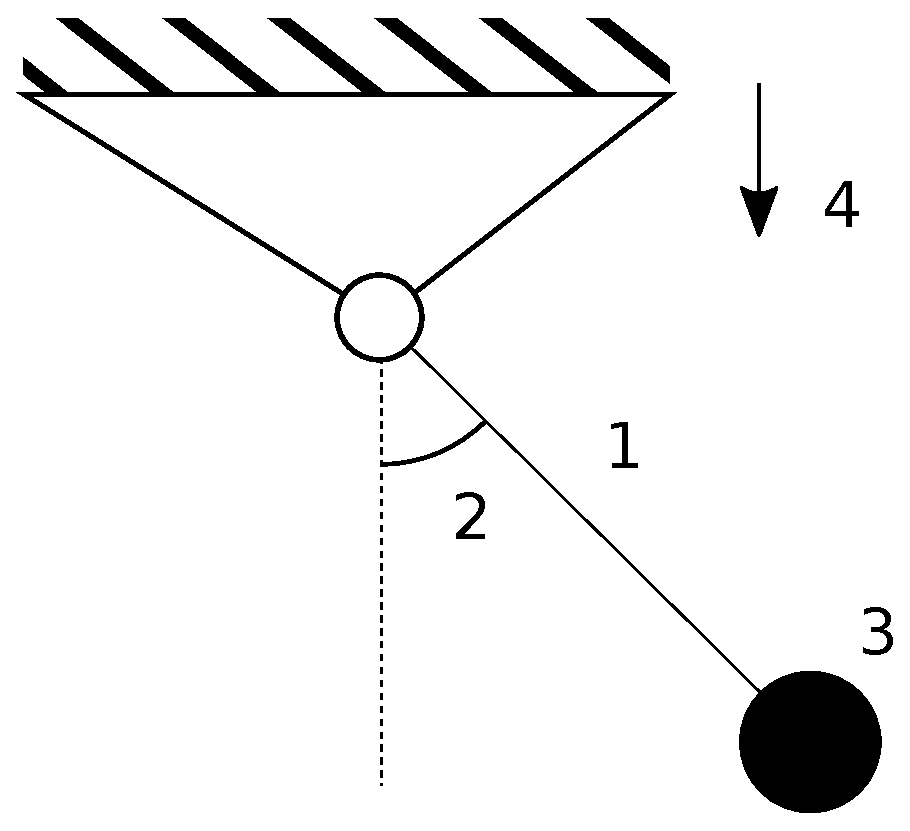
\includegraphics[width=0.2\textwidth]{Figures/Zeichnung-1.eps}}
  \end{center}
  \caption{Schematic representation of the system}
  \label{fig:skizze}
\end{figure}


%\begin{figure}[tb]
%    \centering
%    \def\svgwidth{0.4\textwidth}
%    \input{Figures/zeichnung.pdf_tex}
%    \caption{Schematic representation of the system}
%    \label{fig:skizze}
%\end{figure}



The mechanical system considered here consists of a mass point of mass $m$ attached to an ideal inelastic string of length $l$, which is fixed to a rotating bearing as shown in Figure \ref{fig:skizze}.


Since the system evolves in form of circular movement at constant curvature radius, polar coordinates are used to describe the movement. A free body diagram for the mass $m$ is shown in Figure \ref{fig:free body}. The forces considered here are gravity $F_g = m\cdot g$ and the reactive tension of the string $F_r$. Under this circumstances, moment balances in both radial and tangential direction yield the movement equations:

\begin{equation}
\label{eq: radialbalance}
    m \Ddot{r} = F_r - \cos{\phi}\,F_g = 0
\end{equation}

\begin{equation}
\label{eq: tangentialbalance}
    m\, l \, \Ddot{\phi} = -m\, g \,\sin{\phi}
\end{equation}

Equation \ref{eq: radialbalance} can be simplified for small values of $\phi <<\, 1$ by using the approximation $\sin{\phi} \approx \phi $. This yields the linear movement equation:

\begin{equation}

    \Ddot{\phi} = -\frac{g}{l}\,\phi
\end{equation}





\begin{figure}[h]
  \begin{center}
    {
        \psfragscanon
      \psfrag{1}[c][c]{$\vec{F_r}$}
      \psfrag{2}[c][c]{$\vec{F_g}$}
      \psfrag{3}[c][c]{$\vec{\xi_r}$}
      \psfrag{4}[c][c]{$\vec{\xi_{\phi}}$}
      \psfrag{5}[c][c]{$\phi$}
      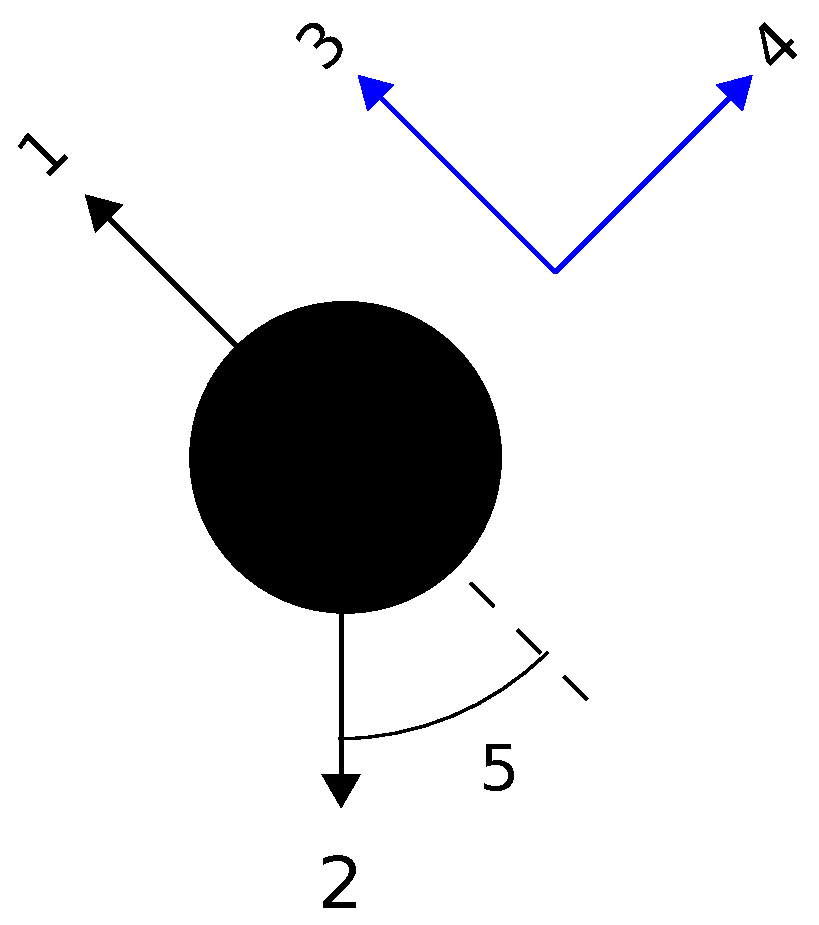
\includegraphics[width=0.2\textwidth]{Figures/Zeichnung2.eps}}
  \end{center}
  \caption{Free body diagram}
  \label{fig:free body}
\end{figure}

\subsection{Derivation of the movement equations using the Lagrange formalism}
\label{sec: lagrange}

In Lagrangian mechanics, the movement equations are derived from a potential called the Lagrangian $l$, which can be written as:

\begin{equation}
\label{eq: Lagrangian}
    L(\Vec{q}, \Vec{\Dot{q}}) = T(\Vec{\Dot{q}}) - V(\Vec{q}),
\end{equation}

where $T$ is the total kinetic energy and $V$ is the potential energy of the system. This function depends on the system describing variables $\Vec{q}$ and their time derivative $\Vec{\Dot{q}}$. The movement equations can then be derived from the Lagrangian equation of second kind:

\begin{equation}
\label{eq: secondKindLagrangian}
    \frac{d}{dt}\left(\frac{\partial L}{\partial \Dot{q}}\right) - \left(\frac{\partial L}{\partial q}  \right) = \Vec{0}.
\end{equation}

Using the minimal coordinate $q$ = $\phi$, the position vector $\Vec{r}$ can be written as:

\begin{equation}
    \Vec{r} = \begin{bmatrix}
        l\,sin(\phi) \\ l\, cos(\phi) 
        \end{bmatrix}
\end{equation}

Furthermore, the kinetic and potential energy are given by:

\begin{equation}
    T = \frac{1}{2}\,\Vec{\Dot{r}}^T\,m\,\Vec{\Dot{r}}
\end{equation}

and 
\begin{equation}
    V = -m\,g\,l\,cos(\phi).
\end{equation}

Hence, the Lagrangian for the mathematical pendulum is given by:
\begin{equation}
    L = \frac{1}{2}\,\Vec{\Dot{r}}^T\,m\,\Vec{\Dot{r}} + m\,g\,l\,cos(\phi)
\end{equation}

and the required derivatives for Equation \ref{eq: Lagrangian} result to:

\begin{equation}
    \left(\frac{\partial L}{\partial \Dot{q}}\right) = \frac{\partial}{\partial \Dot{\phi}} \left( \frac{1}{2}\,m\,l^2\,(sin(\phi)^2 + cos(\phi)^2)\,\Dot{\phi}^2 \right) = m\,l^2\,\Dot{\phi}
\end{equation}

\begin{equation}
\label{eq: LagFirstPart}
    \frac{d}{dt}\left(\frac{\partial L}{\partial \Dot{q}}\right) = m\,l^2\,\Ddot{\phi}
\end{equation}

and 

\begin{equation}
\label{eq: LagSecondPart}
    \left(\frac{\partial L}{\partial q}  \right) = \frac{\partial}{\partial \phi} \left(m\,g\,l\cos(\phi)\right) = -m\,g\,l\,sin(\phi).
\end{equation}

Plugging Equation \ref{eq: LagFirstPart} and \ref{eq: LagSecondPart} into Equation \ref{eq: secondKindLagrangian} yields the movement equation:

\begin{equation}
    m\,l^2\,\Ddot{\phi} + m\,g\,l\,sin(\phi) = 0,
\end{equation}

which is equivalent to Equation \ref{eq: tangentialbalance} derived in Section \ref{sec: NewtonianDerivation}.


\subsection{Analytical solution of the linear movement equation}

The linear movement equation is a ordinary differential equation (ODE) of second order. Due to the presence of constant coefficients, the following approach can be taken:

\begin{equation}
\label{eq: linear}
    \phi (t) = \exp{(\lambda \, t)}.
\end{equation}

This approach leads to the characteristic equation:

\begin{equation}
    \lambda^2 + \frac{g}{l} = 0.
\end{equation}

The solutions to this equation assuming $\frac{g}{l}>0$ are $\lambda_{1,2} = \pm i\,\sqrt{\frac{g}{l}}$. Therefore, a general solution to Equation \ref{eq: linear} is given by:

\begin{equation}
    \phi (t) = A\,\exp{\left(\,i\sqrt{\frac{g}{l}}\,t\right)} + B\, \exp{\left(-\,i\sqrt{\frac{g}{l}}\,t\right)}
\end{equation}

The starting conditions $\Dot{\phi} = 0$ and $\phi = \phi_o$ at $t_o = 0$ yield the form:

\begin{align}
    \phi(t)
    & = \frac{\phi_o}{2}\, \left(\exp{\left(\,i\sqrt{\frac{g}{l}}\,t\right)} + \exp{\left(-\,i\sqrt{\frac{g}{l}}\,t\right)} \right) \\
    & = \phi_o\,\cos{\left(\sqrt{\frac{g}{l}}\,t \right)}
\end{align}

In the following, $\phi_o = 0.0875\,rad$ is assumed. Figure \ref{fig:LinSolutions} (top) shows the course of the analytical solution as a function of time.


\subsection{Numerical solution of the linear equation of movement}

For the numerical solution, three different integration schemes were used: explicit Euler, implicit Euler and the middle point rule. First, the linear equation was expressed in the form of a first order system of PDEs by defining a vector:
\begin{equation}
    \Vec{X} = \begin{bmatrix}
        \phi \\ \Dot{\phi} 
        \end{bmatrix},
\end{equation}

which yields the equivalent representation of Equation \ref{eq: linear} in the form:

\begin{equation}
    \Vec{\Dot{X}} = \begin{bmatrix}
        0 & 1 \\ -\frac{g}{L}\ & 0 
        \end{bmatrix} \, \Vec{X}.
        \label{eq: firstOrderSysLin}
\end{equation}

Equation \ref{eq: firstOrderSysLin} is a first order equation of the form
\begin{equation}
    \Vec{\Dot{X}} = f(t,\Vec{X}),
    \label{eq: GeneralIntForm}
\end{equation}

which can be integrated by using the different standard numerical integration methods.

For the case of explicit Euler, the integration scheme is derived from a Taylor series expansion of the position and the velocity. This yields the following equations:

\begin{equation}
    \Vec{X}(t+\Delta t) = \Vec{X}(t) + [\Dot{\Vec{X}}]_t\,\Delta t + {O(\Delta t^2)},
\end{equation}

which yields a first order approximation of the tangent:

\begin{equation}
    [\Vec{\Dot{X}}]_t = \frac{\Vec{X}(t+\Delta t)-\Vec{X}(t)}{\Delta t} + O\left(\Delta t\right).
    \label{eq: EulerTanApprox}
\end{equation}

Plugging Equation \ref{eq: EulerTanApprox} into Equation \ref{eq: firstOrderSysLin}leads to the integration scheme:

\begin{equation}
    \Vec{X}(t+\Delta t) \approx \Vec{X}(t) + \begin{bmatrix}
        0 & 1 \\ -\frac{g}{L}\ & 0 
        \end{bmatrix} \, \Vec{X}(t) \, \Delta t.
\end{equation}

Contrarily, the implicit Euler method approximates the tangent by taking the values at the end of the interesting time interval. This leads to a first order approximation as well. However, the resulting equation has to be solved explicitly:

\begin{equation}
    \Vec{X}(t+\Delta t) \approx \Vec{X}(t) + \begin{bmatrix}
        0 & 1 \\ -\frac{g}{L}\ & 0 
        \end{bmatrix} \, \Vec{X}(t+\Delta t) \, \Delta t.
\end{equation}

Rearranging the equation leads to a linear equation system of the form:

\begin{equation}
    \left(\vec{I} - \begin{bmatrix}
        0 & 1 \\ -\frac{g}{L}\ & 0 
        \end{bmatrix}\,\Delta t \right)\,\Vec{X}(t+\Delta t) \approx \Vec{X}(t),
\end{equation}
which can be solved by matrix inversion.

Finally, the midpoint rule approximates the tangent by taking its value at the middle of the interesting time interval:

\begin{equation}
    \Vec{\Dot{X}} = f\left( t+\frac{\Delta t}{2}, \Vec{X}(t) + \frac{\Delta t}{2}\,f\left(t, \Vec{X}(t)\right) \right).
\end{equation}

Applying this to Equation \ref{eq: firstOrderSysLin} yields the integration scheme:

\begin{equation}
    \Vec{X}(t+\Delta t) \approx \vec{X}(t) + \begin{bmatrix}
        0 & 1 \\ -\frac{g}{L}\ & 0 
        \end{bmatrix}\,\left(\Vec{X}(t) + \begin{bmatrix}
        0 & 1 \\ -\frac{g}{L}\ & 0 
        \end{bmatrix} \Vec{X}(t)\, \frac{\Delta t}{2} \right).
\end{equation}


\begin{figure}[h]
    \centering
    % This file was created by matlab2tikz.
%
%The latest updates can be retrieved from
%  http://www.mathworks.com/matlabcentral/fileexchange/22022-matlab2tikz-matlab2tikz
%where you can also make suggestions and rate matlab2tikz.
%
\definecolor{mycolor1}{rgb}{1.00000,0.00000,1.00000}%
%
\begin{tikzpicture}

\begin{axis}[%
width=4.521in,
height=1.783in,
at={(0.758in,0.481in)},
scale only axis,
xmin=0,
xmax=30,
xlabel style={font=\color{white!15!black}},
xlabel={Time [s]},
ymin=-0.4,
ymax=0.4,
ylabel style={font=\color{white!15!black}},
ylabel={Angle [rad]},
axis background/.style={fill=white},
legend style={at={(0.03,0.97)}, anchor=north west, legend cell align=left, align=left, draw=white!15!black}
]
\addplot[only marks, mark=*, mark options={}, mark size=0.5000pt, draw=blue] table[row sep=crcr]{%
x	y\\
0	0.0875\\
0.01	0.0875\\
0.02	0.0874141625\\
0.03	0.0872424875\\
0.04	0.0869850592065875\\
0.05	0.0866420460329375\\
0.06	0.0862137005162058\\
0.07	0.0857003591523158\\
0.08	0.0851024421482195\\
0.09	0.0844204530917947\\
0.1	0.0836549785396225\\
0.11	0.0828066875229672\\
0.12	0.0818763309723646\\
0.13	0.080864741061302\\
0.14	0.0797728304695554\\
0.15	0.0786015915668278\\
0.16	0.0773520955174095\\
0.17	0.0760254913066641\\
0.18	0.0746230046902162\\
0.19	0.0731459370667964\\
0.2	0.0715956642757755\\
0.21	0.0699736353204921\\
0.22	0.0682813710185541\\
0.23	0.0665204625803668\\
0.24	0.0646925701172102\\
0.25	0.0627994210802623\\
0.26	0.0608428086320295\\
0.27	0.0588245899517169\\
0.28	0.0567466844761362\\
0.29	0.054611072077813\\
0.3	0.0524197911820186\\
0.31	0.0501749368245159\\
0.32	0.0478786586518637\\
0.33	0.0455331588661866\\
0.34	0.043140690116372\\
0.35	0.0407035533377097\\
0.36	0.0382240955420432\\
0.37	0.0357047075605524\\
0.38	0.0331478217413349\\
0.39	0.0305559096040005\\
0.4	0.0279314794535378\\
0.41	0.0252770739557537\\
0.42	0.0225952676766256\\
0.43	0.0198886645879469\\
0.44	0.0171598955416774\\
0.45	0.0144116157154471\\
0.46	0.0116465020316905\\
0.47	0.00886725055291703\\
0.48	0.00607657385565046\\
0.49	0.00327719838559147\\
0.5	0.000471861796580092\\
0.51	-0.00233668972404755\\
0.52	-0.00514570414109764\\
0.53	-0.00795242626552843\\
0.54	-0.0107541004541968\\
0.55	-0.0135479733126987\\
0.56	-0.016331296398655\\
0.57	-0.0191013289227916\\
0.58	-0.0218553404451611\\
0.59	-0.0245906135638573\\
0.6	-0.0273044465935769\\
0.61	-0.0299941562313903\\
0.62	-0.0326570802070953\\
0.63	-0.0352905799155374\\
0.64	-0.0378920430282964\\
0.65	-0.0404588860821582\\
0.66	-0.0429885570418092\\
0.67	-0.0454785378342136\\
0.68	-0.04792634685216\\
0.69	-0.0503295414244911\\
0.7	-0.0526857202505602\\
0.71	-0.0549925257964919\\
0.72	-0.0572476466508577\\
0.73	-0.0594488198374172\\
0.74	-0.0615938330826122\\
0.75	-0.0636805270355467\\
0.76	-0.0657067974382272\\
0.77	-0.0676705972438858\\
0.78	-0.0695699386812575\\
0.79	-0.0714028952627329\\
0.8	-0.0731676037343621\\
0.81	-0.0748622659657384\\
0.82	-0.0764851507778514\\
0.83	-0.078034595707052\\
0.84	-0.0795090087033395\\
0.85	-0.0809068697612384\\
0.86	-0.0822267324815993\\
0.87	-0.0834672255627245\\
0.88	-0.0846270542192852\\
0.89	-0.0857050015275688\\
0.9	-0.0866999296956634\\
0.91	-0.0876107812572594\\
0.92	-0.0884365801878239\\
0.93	-0.0891764329419751\\
0.94	-0.089829529410962\\
0.95	-0.0903951437992329\\
0.96	-0.0908726354191516\\
0.97	-0.0912614494030032\\
0.98	-0.0915611173315087\\
0.99	-0.0917712577781498\\
1	-0.0918915767686887\\
1.01	-0.0919218681553473\\
1.02	-0.0918620139051957\\
1.03	-0.0917119843023838\\
1.04	-0.0914718380639308\\
1.05	-0.0911417223688773\\
1.06	-0.090721872800683\\
1.07	-0.0902126132028448\\
1.08	-0.0896143554477892\\
1.09	-0.0889275991191815\\
1.1	-0.0881529311078796\\
1.11	-0.0872910251218418\\
1.12	-0.0863426411103872\\
1.13	-0.085308624603288\\
1.14	-0.0841899059652595\\
1.15	-0.0829874995664952\\
1.16	-0.081702502869979\\
1.17	-0.0803360954363881\\
1.18	-0.0788895378474817\\
1.19	-0.0773641705489522\\
1.2	-0.0757614126137943\\
1.21	-0.0740827604273279\\
1.22	-0.0723297862950874\\
1.23	-0.0705041369748677\\
1.24	-0.0686075321342924\\
1.25	-0.0666417627353449\\
1.26	-0.0646086893473736\\
1.27	-0.0625102403901589\\
1.28	-0.0603484103086945\\
1.29	-0.0581252576814073\\
1.3	-0.0558429032636072\\
1.31	-0.0535035279680217\\
1.32	-0.0511093707843347\\
1.33	-0.048662726639711\\
1.34	-0.0461659442023478\\
1.35	-0.0436214236301511\\
1.36	-0.0410316142666919\\
1.37	-0.0383990122866515\\
1.38	-0.0357261582930155\\
1.39	-0.0330156348683263\\
1.4	-0.0302700640823517\\
1.41	-0.0274921049585712\\
1.42	-0.0246844509019259\\
1.43	-0.0218498270903163\\
1.44	-0.0189909878323718\\
1.45	-0.0161107138940518\\
1.46	-0.0132118097966683\\
1.47	-0.0102971010889546\\
1.48	-0.00736943159583043\\
1.49	-0.00443166064653799\\
1.5	-0.00148666028485004\\
1.51	0.00146268753593216\\
1.52	0.0044134937704538\\
1.53	0.00736286510850269\\
1.54	0.0103079068091628\\
1.55	0.0132457255391514\\
1.56	0.0161734322125602\\
1.57	0.0190881448292152\\
1.58	0.0219869913088696\\
1.59	0.0248671123184466\\
1.6	0.0277256640895495\\
1.61	0.0305598212234681\\
1.62	0.0333667794809148\\
1.63	0.0361437585537413\\
1.64	0.038888004815897\\
1.65	0.0415967940509115\\
1.66	0.0442674341532016\\
1.67	0.0468972678005277\\
1.68	0.0494836750949496\\
1.69	0.0520240761696591\\
1.7	0.0545159337591005\\
1.71	0.0569567557298195\\
1.72	0.0593440975695208\\
1.73	0.0616755648318511\\
1.74	0.0639488155344657\\
1.75	0.0661615625079803\\
1.76	0.0683115756934556\\
1.77	0.0703966843861106\\
1.78	0.0724147794230102\\
1.79	0.0743638153125271\\
1.8	0.07624181230343\\
1.81	0.0780468583915114\\
1.82	0.079777111261723\\
1.83	0.0814308001638526\\
1.84	0.0830062277198345\\
1.85	0.0845017716608556\\
1.86	0.0859158864924835\\
1.87	0.0872471050861122\\
1.88	0.0884940401950917\\
1.89	0.0896553858939817\\
1.9	0.0907299189394404\\
1.91	0.091716500051337\\
1.92	0.0926140751127541\\
1.93	0.0934216762876208\\
1.94	0.0941384230548019\\
1.95	0.0947635231575449\\
1.96	0.095296273467271\\
1.97	0.0957360607607797\\
1.98	0.0960823624100169\\
1.99	0.0963347469836478\\
2	0.0964928747597545\\
2.01	0.0965564981490702\\
2.02	0.0965254620282467\\
2.03	0.0963997039827388\\
2.04	0.0961792544589813\\
2.05	0.0958642368256167\\
2.06	0.0954548673436278\\
2.07	0.094951455045313\\
2.08	0.0943544015221341\\
2.09	0.0936642006215558\\
2.1	0.0928814380530842\\
2.11	0.0920067909038029\\
2.12	0.0910410270637915\\
2.13	0.0899850045619035\\
2.14	0.0888396708124659\\
2.15	0.0876060617735531\\
2.16	0.0862853010175732\\
2.17	0.0848785987149935\\
2.18	0.0833872505321156\\
2.19	0.0818126364438982\\
2.2	0.0801562194629089\\
2.21	0.0784195442855681\\
2.22	0.0766042358569341\\
2.23	0.0747119978553561\\
2.24	0.0727446110984023\\
2.25	0.0707039318715525\\
2.26	0.0685918901812151\\
2.27	0.0664104879337118\\
2.28	0.0641617970419406\\
2.29	0.0618479574615065\\
2.3	0.0594711751581743\\
2.31	0.0570337200085723\\
2.32	0.0545379236361401\\
2.33	0.0519861771843795\\
2.34	0.0493809290295319\\
2.35	0.0467246824348664\\
2.36	0.044019993148823\\
2.37	0.0412694669493109\\
2.38	0.0384757571365198\\
2.39	0.0356415619766515\\
2.4	0.0327696220990322\\
2.41	0.0298627178491139\\
2.42	0.0269236665999164\\
2.43	0.0239553200245089\\
2.44	0.0209605613321669\\
2.45	0.0179423024708808\\
2.46	0.0149034812989279\\
2.47	0.0118470587282511\\
2.48	0.00877601584241997\\
2.49	0.00569335099197647\\
2.5	0.00260207686999155\\
2.51	-0.000494782429316498\\
2.52	-0.00359419436603401\\
2.53	-0.00669312092118836\\
2.54	-0.00978852157166963\\
2.55	-0.0128773562705272\\
2.56	-0.015956588429723\\
2.57	-0.0190231879024174\\
2.58	-0.0220741339618622\\
2.59	-0.0251064182739748\\
2.6	-0.0281170478606707\\
2.61	-0.03110304805104\\
2.62	-0.0340614654174578\\
2.63	-0.0369893706937377\\
2.64	-0.0398838616724429\\
2.65	-0.0427420660784977\\
2.66	-0.0455611444162517\\
2.67	-0.0483382927871828\\
2.68	-0.0510707456754415\\
2.69	-0.053755778698476\\
2.7	-0.0563907113200029\\
2.71	-0.0589729095226266\\
2.72	-0.0614997884374453\\
2.73	-0.0639688149280224\\
2.74	-0.0663775101261423\\
2.75	-0.0687234519168178\\
2.76	-0.0710042773700596\\
2.77	-0.073217685116971\\
2.78	-0.0753614376677824\\
2.79	-0.077433363669494\\
2.8	-0.0794313601008535\\
2.81	-0.0813533944024533\\
2.82	-0.0831975065397941\\
2.83	-0.0849618109972261\\
2.84	-0.0866444987007426\\
2.85	-0.0882438388676707\\
2.86	-0.0897581807813735\\
2.87	-0.0911859554891471\\
2.88	-0.0925256774215741\\
2.89	-0.0937759459316663\\
2.9	-0.0949354467522079\\
2.91	-0.0960029533697906\\
2.92	-0.0969773283141093\\
2.93	-0.0978575243611723\\
2.94	-0.0986425856491592\\
2.95	-0.0993316487057477\\
2.96	-0.0999239433858144\\
2.97	-0.100418793718501\\
2.98	-0.100815618662726\\
2.99	-0.101113932770313\\
3	-0.101313346755992\\
3.01	-0.101413567973623\\
3.02	-0.101414400798086\\
3.03	-0.101315746912368\\
3.04	-0.101117605499466\\
3.05	-0.100820073338844\\
3.06	-0.100423344807226\\
3.07	-0.0999277117836636\\
3.08	-0.0993335634588448\\
3.09	-0.0986413860487663\\
3.1	-0.0978517624129347\\
3.11	-0.0969653715773892\\
3.12	-0.0959829881629166\\
3.13	-0.0949054817189266\\
3.14	-0.0937338159635487\\
3.15	-0.0924690479306046\\
3.16	-0.0911123270242003\\
3.17	-0.0896648939817761\\
3.18	-0.0881280797465411\\
3.19	-0.0865033042503099\\
3.2	-0.0847920751078475\\
3.21	-0.0829959862239154\\
3.22	-0.0811167163143026\\
3.23	-0.0791560273422041\\
3.24	-0.0771157628714013\\
3.25	-0.0749978463377758\\
3.26	-0.0728042792407734\\
3.27	-0.0705371392565137\\
3.28	-0.0681985782743187\\
3.29	-0.0657908203585132\\
3.3	-0.0633161596374205\\
3.31	-0.0607769581215561\\
3.32	-0.0581756434530874\\
3.33	-0.0555147065887015\\
3.34	-0.0527966994180881\\
3.35	-0.0500242323203112\\
3.36	-0.0471999716604051\\
3.37	-0.0443266372285928\\
3.38	-0.0414069996245817\\
3.39	-0.0384438775894493\\
3.4	-0.0354401352876851\\
3.41	-0.0323986795420058\\
3.42	-0.0293224570236092\\
3.43	-0.0262144514005819\\
3.44	-0.0230776804472145\\
3.45	-0.019915193117023\\
3.46	-0.0167300665823129\\
3.47	-0.013525403243155\\
3.48	-0.0103043277086798\\
3.49	-0.00706998375362304\\
3.5	-0.0038255312530841\\
3.51	-0.000574143098482861\\
3.52	0.00268099790227766\\
3.53	0.00593670213741779\\
3.54	0.00918977631361578\\
3.55	0.012437026585017\\
3.56	0.0156752616858545\\
3.57	0.0189012960636121\\
3.58	0.0221119530096559\\
3.59	0.0253040677842613\\
3.6	0.0284744907329643\\
3.61	0.0316200903911708\\
3.62	0.0347377565739684\\
3.63	0.0378244034480922\\
3.64	0.0408769725830169\\
3.65	0.0438924359781591\\
3.66	0.0468677990631973\\
3.67	0.0498001036685409\\
3.68	0.0526864309630036\\
3.69	0.0555239043557674\\
3.7	0.0583096923597565\\
3.71	0.0610410114135725\\
3.72	0.0637151286591837\\
3.73	0.0663293646725982\\
3.74	0.068881096144798\\
3.75	0.0713677585102539\\
3.76	0.0737868485203919\\
3.77	0.0761359267594312\\
3.78	0.0784126201000721\\
3.79	0.080614624096562\\
3.8	0.0827397053127337\\
3.81	0.0847857035826666\\
3.82	0.0867505342016878\\
3.83	0.0886321900454944\\
3.84	0.0904287436152491\\
3.85	0.0921383490065692\\
3.86	0.0937592438004027\\
3.87	0.0952897508738608\\
3.88	0.0967282801291507\\
3.89	0.0980733301388333\\
3.9	0.0993234897057093\\
3.91	0.100477439335719\\
3.92	0.101533952622327\\
3.93	0.102491897540948\\
3.94	0.103350237652045\\
3.95	0.104108033211655\\
3.96	0.104764442188128\\
3.97	0.105318721184021\\
3.98	0.105770226262127\\
3.99	0.106118413674752\\
4	0.106362840495413\\
4.01	0.10650316515226\\
4.02	0.10653914786258\\
4.03	0.106470650967886\\
4.04	0.106297639169139\\
4.05	0.106020179661793\\
4.06	0.105638442170421\\
4.07	0.105152698882801\\
4.08	0.104563324283412\\
4.09	0.103870794886419\\
4.1	0.103075688868305\\
4.11	0.102178685600406\\
4.12	0.101180565081728\\
4.13	0.100082207272475\\
4.14	0.0988845913288778\\
4.15	0.097588794739946\\
4.16	0.0961959923669205\\
4.17	0.0947074553862552\\
4.18	0.0931245501370779\\
4.19	0.0914487368741668\\
4.2	0.0896815684275711\\
4.21	0.0878246887701019\\
4.22	0.0858798314940052\\
4.23	0.0838488181982251\\
4.24	0.0817335567877493\\
4.25	0.0795360396866211\\
4.26	0.0772583419662841\\
4.27	0.0749026193910145\\
4.28	0.072471106382276\\
4.29	0.069966113903915\\
4.3	0.0673900272701929\\
4.31	0.064745303878731\\
4.32	0.0620344708705171\\
4.33	0.0592601227191982\\
4.34	0.0564249187519553\\
4.35	0.0535315806043248\\
4.36	0.0505828896113987\\
4.37	0.0475816841378998\\
4.38	0.044530856849692\\
4.39	0.041433351929345\\
4.4	0.0382921622384285\\
4.41	0.0351103264292692\\
4.42	0.0318909260089541\\
4.43	0.0286370823584118\\
4.44	0.0253519537094547\\
4.45	0.0220387320827041\\
4.46	0.0187006401893645\\
4.47	0.0153409282998517\\
4.48	0.0119628710823132\\
4.49	0.00856976441411252\\
4.5	0.00516492216938009\\
4.51	0.00175167298575742\\
4.52	-0.00166664298651342\\
4.53	-0.00508667734998328\\
4.54	-0.00850507673668337\\
4.55	-0.0119184860929031\\
4.56	-0.0153235519688442\\
4.57	-0.0187169258099281\\
4.58	-0.0220952672465306\\
4.59	-0.0254552473789136\\
4.6	-0.0287935520541277\\
4.61	-0.0321068851316631\\
4.62	-0.0353919717346334\\
4.63	-0.0386455614832895\\
4.64	-0.041864431707674\\
4.65	-0.0450453906362434\\
4.66	-0.0481852805573075\\
4.67	-0.0512809809501575\\
4.68	-0.0543294115827807\\
4.69	-0.0573275355730919\\
4.7	-0.0602723624106403\\
4.71	-0.0631609509357915\\
4.72	-0.0659904122734179\\
4.73	-0.0687579127181763\\
4.74	-0.0714606765684945\\
4.75	-0.0740959889064361\\
4.76	-0.0766611983206641\\
4.77	-0.0791537195697748\\
4.78	-0.0815710361833329\\
4.79	-0.0839107029979932\\
4.8	-0.0861703486261575\\
4.81	-0.0883476778546808\\
4.82	-0.0904404739712019\\
4.83	-0.0924466010157475\\
4.84	-0.0943640059553274\\
4.85	-0.0961907207793108\\
4.86	-0.0979248645134521\\
4.87	-0.0995646451505088\\
4.88	-0.101108361495478\\
4.89	-0.102554404923554\\
4.9	-0.103901261049004\\
4.91	-0.105147511303223\\
4.92	-0.106291834420353\\
4.93	-0.107333007828895\\
4.94	-0.10826990894787\\
4.95	-0.109101516386166\\
4.96	-0.109826911043783\\
4.97	-0.110445277113826\\
4.98	-0.110955902984134\\
4.99	-0.111358182037594\\
5	-0.111651613350227\\
5.01	-0.111835802286281\\
5.02	-0.111910460989638\\
5.03	-0.111875408770952\\
5.04	-0.111730572390035\\
5.05	-0.111475986233114\\
5.06	-0.111111792384679\\
5.07	-0.110638240593749\\
5.08	-0.110055688134489\\
5.09	-0.109364599561207\\
5.1	-0.108565546357865\\
5.11	-0.107659206482354\\
5.12	-0.106646363805865\\
5.13	-0.105527907447817\\
5.14	-0.104304831006876\\
5.15	-0.102978231688728\\
5.16	-0.101549309331363\\
5.17	-0.100019365328711\\
5.18	-0.0983898014536048\\
5.19	-0.0966621185811112\\
5.2	-0.0948379153133917\\
5.21	-0.0929188865073441\\
5.22	-0.090906821706374\\
5.23	-0.0888036034777403\\
5.24	-0.0866112056570126\\
5.25	-0.0843316915012732\\
5.26	-0.0819672117527843\\
5.27	-0.0795200026149327\\
5.28	-0.0769923836423516\\
5.29	-0.0743867555472052\\
5.3	-0.0717055979237057\\
5.31	-0.0689514668930143\\
5.32	-0.0661269926707598\\
5.33	-0.0632348770594833\\
5.34	-0.0602778908683968\\
5.35	-0.0572588712629149\\
5.36	-0.0541807190464911\\
5.37	-0.0510463958773584\\
5.38	-0.047858921422841\\
5.39	-0.044621370453968\\
5.4	-0.0413368698831792\\
5.41	-0.038008595747975\\
5.42	-0.0346397701434155\\
5.43	-0.0312336581064271\\
5.44	-0.0277935644549281\\
5.45	-0.0243228305848267\\
5.46	-0.020824831227995\\
5.47	-0.0173029711743596\\
5.48	-0.0137606819612895\\
5.49	-0.0102014185334974\\
5.5	-0.0066286558767012\\
5.51	-0.00304588562832368\\
5.52	0.000543387331468882\\
5.53	0.00413564830506283\\
5.54	0.0077273762156846\\
5.55	0.0113150470553191\\
5.56	0.014895137338886\\
5.57	0.0184641275612917\\
5.58	0.0220185056539679\\
5.59	0.0255547704375065\\
5.6	0.0290694350669985\\
5.61	0.0325590304666913\\
5.62	0.0360201087505835\\
5.63	0.0394492466255878\\
5.64	0.0428430487739077\\
5.65	0.046198151211288\\
5.66	0.0495112246178211\\
5.67	0.0527789776380159\\
5.68	0.0559981601468606\\
5.69	0.0591655664786424\\
5.7	0.0622780386153201\\
5.71	0.0653324693312823\\
5.72	0.0683258052913629\\
5.73	0.0712550500990295\\
5.74	0.0741172672917052\\
5.75	0.0769095832802338\\
5.76	0.0796291902295493\\
5.77	0.0822733488776668\\
5.78	0.0848393912901692\\
5.79	0.0873247235474225\\
5.8	0.0897268283618202\\
5.81	0.0920432676224179\\
5.82	0.0942716848643926\\
5.83	0.0964098076608298\\
5.84	0.0984554499344149\\
5.85	0.100406514186685\\
5.86	0.102260993642569\\
5.87	0.104016974308036\\
5.88	0.10567263693874\\
5.89	0.107226258917647\\
5.9	0.108676216039718\\
5.91	0.110020984201791\\
5.92	0.111259140995928\\
5.93	0.112389367204564\\
5.94	0.113410448195882\\
5.95	0.114321275217973\\
5.96	0.115120846590384\\
5.97	0.115808268791805\\
5.98	0.116382757442722\\
5.99	0.116843638181954\\
6	0.117190347436135\\
6.01	0.117422433081259\\
6.02	0.117539554995548\\
6.03	0.117541485502984\\
6.04	0.11742810970697\\
6.05	0.117199425713678\\
6.06	0.116855544744763\\
6.07	0.116396691139223\\
6.08	0.115823202244288\\
6.09	0.115135528195346\\
6.1	0.114334231585002\\
6.11	0.113419987021498\\
6.12	0.112393580576809\\
6.13	0.111255909124853\\
6.14	0.11000797957035\\
6.15	0.108650907968996\\
6.16	0.107185918539684\\
6.17	0.105614342569654\\
6.18	0.103937617213536\\
6.19	0.102157284187358\\
6.2	0.100274988358693\\
6.21	0.0982924762342407\\
6.22	0.0962115943462082\\
6.23	0.0940342875389899\\
6.24	0.0917625971577181\\
6.25	0.0893986591403704\\
6.26	0.0869447020152111\\
6.27	0.084403044805435\\
6.28	0.081776094842982\\
6.29	0.0790663454935749\\
6.3	0.0762763737951268\\
6.31	0.0734088380117496\\
6.32	0.0704664751056793\\
6.33	0.0674520981295195\\
6.34	0.064368593541281\\
6.35	0.0612189184447774\\
6.36	0.0580060977580099\\
6.37	0.054733221312248\\
6.38	0.0514034408845855\\
6.39	0.0480199671668157\\
6.4	0.0445860666735382\\
6.41	0.0411050585924699\\
6.42	0.037580311579995\\
6.43	0.0340152405050408\\
6.44	0.0304133031444267\\
6.45	0.0267779968328771\\
6.46	0.0231128550709428\\
6.47	0.0194214440941155\\
6.48	0.0157073594064635\\
6.49	0.0119742222821553\\
6.5	0.0082256762382693\\
6.51	0.00446538348232451\\
6.52	0.000697021337989984\\
6.53	-0.00307572134754071\\
6.54	-0.00684914781100396\\
6.55	-0.0106195569918253\\
6.56	-0.014383247158644\\
6.57	-0.0181365195400538\\
6.58	-0.0218756819560009\\
6.59	-0.0255970524462792\\
6.6	-0.0292969628925587\\
6.61	-0.0329717626303884\\
6.62	-0.0366178220476205\\
6.63	-0.0402315361657121\\
6.64	-0.0438093282003751\\
6.65	-0.0473476530980595\\
6.66	-0.0508430010447793\\
6.67	-0.0542919009438099\\
6.68	-0.0576909238588156\\
6.69	-0.0610366864189955\\
6.7	-0.0643258541828698\\
6.71	-0.0675551449573671\\
6.72	-0.070721332068911\\
6.73	-0.0738212475832517\\
6.74	-0.0768517854708328\\
6.75	-0.0798099047145348\\
6.76	-0.0826926323566898\\
6.77	-0.0854970664823199\\
6.78	-0.0882203791356081\\
6.79	-0.0908598191666772\\
6.8	-0.0934127150058142\\
6.81	-0.0958764773623487\\
6.82	-0.0982486018454625\\
6.83	-0.100526671504284\\
6.84	-0.102708359284695\\
6.85	-0.10479143040036\\
6.86	-0.106773744615567\\
6.87	-0.108653258437551\\
6.88	-0.110428027216067\\
6.89	-0.112096207148056\\
6.9	-0.113656057185347\\
6.91	-0.115105940843424\\
6.92	-0.116444327909403\\
6.93	-0.117669796047415\\
6.94	-0.118781032299748\\
6.95	-0.119776834482158\\
6.96	-0.120656112471882\\
6.97	-0.121417889386979\\
6.98	-0.122061302655741\\
6.99	-0.122585604975014\\
7	-0.122990165156382\\
7.01	-0.12327446885927\\
7.02	-0.123438119210139\\
7.03	-0.123480837307057\\
7.04	-0.12340246260903\\
7.05	-0.123202953209605\\
7.06	-0.122882385994361\\
7.07	-0.122440956682018\\
7.08	-0.121878979749014\\
7.09	-0.121196888237505\\
7.1	-0.120395233446863\\
7.11	-0.119474684508859\\
7.12	-0.118436027846845\\
7.13	-0.117280166519327\\
7.14	-0.116008119448491\\
7.15	-0.1146210205343\\
7.16	-0.113120117654929\\
7.17	-0.111506771554415\\
7.18	-0.109782454618481\\
7.19	-0.107948749539652\\
7.2	-0.106007347872843\\
7.21	-0.103960048482735\\
7.22	-0.101808755884364\\
7.23	-0.0995554784784314\\
7.24	-0.0972023266829761\\
7.25	-0.0947515109631335\\
7.26	-0.092205339760815\\
7.27	-0.0895662173262416\\
7.28	-0.0868366414533628\\
7.29	-0.084019201121287\\
7.3	-0.0811165740439454\\
7.31	-0.0781315241303039\\
7.32	-0.0750668988575252\\
7.33	-0.0719256265595747\\
7.34	-0.068710713633845\\
7.35	-0.0654252416684603\\
7.36	-0.0620723644930009\\
7.37	-0.0586553051554647\\
7.38	-0.0551773528283608\\
7.39	-0.0516418596468994\\
7.4	-0.0480522374823134\\
7.41	-0.0444119546534138\\
7.42	-0.0407245325795441\\
7.43	-0.0369935423781593\\
7.44	-0.0332226014103141\\
7.45	-0.0294153697773958\\
7.46	-0.025575546772494\\
7.47	-0.0217068672898406\\
7.48	-0.0178130981958034\\
7.49	-0.0138980346649549\\
7.5	-0.00996549648477626\\
7.51	-0.00601932433259131\\
7.52	-0.00206337602835479\\
7.53	0.001898477233052\\
7.54	0.0058623546663426\\
7.55	0.00982436969346758\\
7.56	0.0137806337506649\\
7.57	0.0177272601011929\\
7.58	0.0216603676500115\\
7.59	0.0255760847566708\\
7.6	0.0294705530426655\\
7.61	0.0333399311895139\\
7.62	0.0371803987238274\\
7.63	0.040988159785644\\
7.64	0.0447594468763125\\
7.65	0.0484905245822314\\
7.66	0.0521776932707645\\
7.67	0.0558172927546825\\
7.68	0.0594057059215019\\
7.69	0.0629393623241289\\
7.7	0.0664147417292469\\
7.71	0.069828377619925\\
7.72	0.0731768606489667\\
7.73	0.0764568420395632\\
7.74	0.0796650369298631\\
7.75	0.0827982276581221\\
7.76	0.085853266985153\\
7.77	0.0888270812508513\\
7.78	0.0917166734616371\\
7.79	0.0945191263057159\\
7.8	0.0972316050931287\\
7.81	0.0998513606176357\\
7.82	0.102375731937546\\
7.83	0.104802149072691\\
7.84	0.107128135614805\\
7.85	0.109351311248679\\
7.86	0.111469394181514\\
7.87	0.113480203478015\\
7.88	0.115381661298823\\
7.89	0.11717179504002\\
7.9	0.118848739371482\\
7.91	0.120410738172011\\
7.92	0.121856146359215\\
7.93	0.123183431612273\\
7.94	0.124391175985753\\
7.95	0.125478077412821\\
7.96	0.126442951096247\\
7.97	0.127284730785731\\
7.98	0.128002469940189\\
7.99	0.128595342773747\\
8	0.129062645184294\\
8.01	0.129403795563579\\
8.02	0.129618335487939\\
8.03	0.12970593028885\\
8.04	0.129666369502648\\
8.05	0.129499567198833\\
8.06	0.129205562186536\\
8.07	0.128784518098816\\
8.08	0.128236723354592\\
8.09	0.127562590998112\\
8.1	0.126762658416022\\
8.11	0.125837586932163\\
8.12	0.124788161280397\\
8.13	0.123615288955851\\
8.14	0.122319999445089\\
8.15	0.120903443335862\\
8.16	0.119366891307178\\
8.17	0.117711733000582\\
8.18	0.115939475773614\\
8.19	0.114051743336573\\
8.2	0.112050274273797\\
8.21	0.109936920450808\\
8.22	0.107713645308757\\
8.23	0.105382522047743\\
8.24	0.102945731700681\\
8.25	0.100405561099491\\
8.26	0.0977644007355022\\
8.27	0.0950247425160749\\
8.28	0.092189177419526\\
8.29	0.0892603930505688\\
8.3	0.0862411710985631\\
8.31	0.0831343847009748\\
8.32	0.0799429957145388\\
8.33	0.0766700518967111\\
8.34	0.0733186840000875\\
8.35	0.0698921027825531\\
8.36	0.0663935959360148\\
8.37	0.0628265249366467\\
8.38	0.0591943218196654\\
8.39	0.0555004858817212\\
8.4	0.051748580314072\\
8.41	0.0479422287697727\\
8.42	0.0440851118681854\\
8.43	0.0401809636401749\\
8.44	0.0362335679174218\\
8.45	0.0322467546693376\\
8.46	0.0282243962911264\\
8.47	0.0241704038465846\\
8.48	0.0200887232692813\\
8.49	0.0159833315258044\\
8.5	0.0118582327448003\\
8.51	0.00771745431556948\\
8.52	0.00356504296001597\\
8.53	-0.000594939218221113\\
8.54	-0.00475841870360197\\
8.55	-0.00892131455360975\\
8.56	-0.0130795423948693\\
8.57	-0.0172290184265518\\
8.58	-0.0213656634271448\\
8.59	-0.0254854067606615\\
8.6	-0.0295841903783561\\
8.61	-0.0336579728120185\\
8.62	-0.0377027331549197\\
8.63	-0.0417144750264924\\
8.64	-0.0456892305168401\\
8.65	-0.0496230641071867\\
8.66	-0.0535120765623964\\
8.67	-0.0573524087917169\\
8.68	-0.0611402456739297\\
8.69	-0.0648718198431178\\
8.7	-0.0685434154312998\\
8.71	-0.0721513717642157\\
8.72	-0.0756920870065935\\
8.73	-0.0791620217532706\\
8.74	-0.0825577025625943\\
8.75	-0.085875725428578\\
8.76	-0.0891127591883477\\
8.77	-0.0922655488614721\\
8.78	-0.0953309189178326\\
8.79	-0.0983057764707601\\
8.8	-0.101187114392229\\
8.81	-0.10397201434698\\
8.82	-0.106657649742513\\
8.83	-0.109241288591971\\
8.84	-0.111720296287032\\
8.85	-0.114092138277984\\
8.86	-0.116354382658278\\
8.87	-0.118504702650922\\
8.88	-0.120540878994178\\
8.89	-0.122460802224133\\
8.9	-0.124262474851795\\
8.91	-0.125944013432475\\
8.92	-0.127503650525326\\
8.93	-0.128939736540999\\
8.94	-0.130250741475507\\
8.95	-0.131435256528468\\
8.96	-0.132491995604042\\
8.97	-0.133419796692962\\
8.98	-0.134217623134193\\
8.99	-0.134884564754869\\
9	-0.135419838887251\\
9.01	-0.135822791261607\\
9.02	-0.136092896774016\\
9.03	-0.136229760128197\\
9.04	-0.136233116350642\\
9.05	-0.136102831178402\\
9.06	-0.135838901319022\\
9.07	-0.135441454582255\\
9.08	-0.134910749883295\\
9.09	-0.13424717711739\\
9.1	-0.133451256905849\\
9.11	-0.132523640213556\\
9.12	-0.131465107838238\\
9.13	-0.130276569771871\\
9.14	-0.128959064434714\\
9.15	-0.127513757782612\\
9.16	-0.125941942288298\\
9.17	-0.1242450357976\\
9.18	-0.122424580261518\\
9.19	-0.120482240345317\\
9.2	-0.118419801915881\\
9.21	-0.116239170408665\\
9.22	-0.11394236907577\\
9.23	-0.111531537116704\\
9.24	-0.109008927693575\\
9.25	-0.106376905832534\\
9.26	-0.103637946213426\\
9.27	-0.100794630849696\\
9.28	-0.0978496466607312\\
9.29	-0.0948057829389025\\
9.3	-0.0916659287136996\\
9.31	-0.0884330700154336\\
9.32	-0.0851102870410994\\
9.33	-0.0817007512250802\\
9.34	-0.0782077222174736\\
9.35	-0.0746345447729152\\
9.36	-0.0709846455528615\\
9.37	-0.0672615298443855\\
9.38	-0.0634687781986222\\
9.39	-0.0596100429920815\\
9.4	-0.055689044914128\\
9.41	-0.0517095693839993\\
9.42	-0.0476754629008098\\
9.43	-0.0435906293300546\\
9.44	-0.0394590261301937\\
9.45	-0.03528466052296\\
9.46	-0.0310715856110926\\
9.47	-0.0268238964472522\\
9.48	-0.0225457260579273\\
9.49	-0.0182412414261876\\
9.5	-0.0139146394371851\\
9.51	-0.00957014279034357\\
9.52	-0.00521199588221411\\
9.53	-0.000844460664007329\\
9.54	0.0035281875221599\\
9.55	0.00790166412423853\\
9.56	0.0122716795743579\\
9.57	0.0166339434919714\\
9.58	0.0209841688919225\\
9.59	0.0253180763933079\\
9.6	0.0296313984250104\\
9.61	0.033919883423771\\
9.62	0.0381793000206767\\
9.63	0.0424054412119437\\
9.64	0.0465941285098904\\
9.65	0.0507412160700082\\
9.66	0.0548425947900577\\
9.67	0.0588941963771426\\
9.68	0.0628919973787385\\
9.69	0.0668320231736883\\
9.7	0.0707103519192097\\
9.71	0.0745231184499976\\
9.72	0.0782665181255528\\
9.73	0.0819368106219085\\
9.74	0.0855303236639831\\
9.75	0.0890434566948376\\
9.76	0.0924726844781777\\
9.77	0.0958145606305002\\
9.78	0.0990657210793496\\
9.79	0.10222288744422\\
9.8	0.105282870336712\\
9.81	0.108242572576622\\
9.82	0.111098992320731\\
9.83	0.113849226101142\\
9.84	0.116490471770087\\
9.85	0.119020031348226\\
9.86	0.121435313773559\\
9.87	0.123733837548139\\
9.88	0.125913233279908\\
9.89	0.127971246117041\\
9.9	0.129905738072328\\
9.91	0.131714690235173\\
9.92	0.133396204868969\\
9.93	0.134948507391645\\
9.94	0.136369948237344\\
9.95	0.137659004597292\\
9.96	0.13881428203802\\
9.97	0.139834515995237\\
9.98	0.140718573141775\\
9.99	0.141465452628121\\
10	0.142074287194216\\
10.01	0.142544344151282\\
10.02	0.142875026232611\\
10.03	0.143065872312328\\
10.04	0.14311655799131\\
10.05	0.143026896049554\\
10.06	0.142796836764408\\
10.07	0.142426468094238\\
10.08	0.141916015727202\\
10.09	0.141265842994965\\
10.1	0.1404764506513\\
10.11	0.139548476515657\\
10.12	0.138482694981925\\
10.13	0.137280016392731\\
10.14	0.13594148627976\\
10.15	0.134468284470708\\
10.16	0.132861724063615\\
10.17	0.131123250269457\\
10.18	0.129254439123992\\
10.19	0.127256996070012\\
10.2	0.125132754411252\\
10.21	0.122883673639348\\
10.22	0.120511837635366\\
10.23	0.118019452747543\\
10.24	0.115408845747001\\
10.25	0.112682461663313\\
10.26	0.109842861501947\\
10.27	0.10689271984569\\
10.28	0.103834822342299\\
10.29	0.10067206308074\\
10.3	0.0974074418584624\\
10.31	0.0940440613423029\\
10.32	0.0905851241256803\\
10.33	0.0870339296848809\\
10.34	0.0833938712373143\\
10.35	0.0796684325047267\\
10.36	0.0758611843844553\\
10.37	0.0719757815318968\\
10.38	0.0680159588574572\\
10.39	0.0639855279413348\\
10.4	0.0598883733695732\\
10.41	0.0557284489949011\\
10.42	0.0515097741259535\\
10.43	0.0472364296485419\\
10.44	0.0429125540827128\\
10.45	0.0385423395793984\\
10.46	0.0341300278605289\\
10.47	0.0296799061065319\\
10.48	0.0251963027952039\\
10.49	0.0206835834959853\\
10.5	0.0161461466237246\\
10.51	0.0115884191560543\\
10.52	0.00701485231854619\\
10.53	0.00242991724184597\\
10.54	-0.00216189940497874\\
10.55	-0.0067560998006177\\
10.56	-0.0113481793729404\\
10.57	-0.0159336312113587\\
10.58	-0.0205079504858121\\
10.59	-0.0250666388680471\\
10.6	-0.0296052089508556\\
10.61	-0.0341191886609346\\
10.62	-0.0386041256610327\\
10.63	-0.0430555917370545\\
10.64	-0.0474691871658028\\
10.65	-0.0518405450590571\\
10.66	-0.0561653356797016\\
10.67	-0.0604392707256433\\
10.68	-0.0646581075772832\\
10.69	-0.0688176535043412\\
10.7	-0.0729137698278659\\
10.71	-0.0769423760333029\\
10.72	-0.0808994538305387\\
10.73	-0.0847810511568858\\
10.74	-0.0885832861190252\\
10.75	-0.0923023508699797\\
10.76	-0.0959345154172514\\
10.77	-0.0994761313583196\\
10.78	-0.102923635539764\\
10.79	-0.106273553636345\\
10.8	-0.109522503646462\\
10.81	-0.112667199300462\\
10.82	-0.115704453378384\\
10.83	-0.118631180933793\\
10.84	-0.121444402420437\\
10.85	-0.124141246718586\\
10.86	-0.12671895405796\\
10.87	-0.129174878834303\\
10.88	-0.131506492316715\\
10.89	-0.133711385242991\\
10.9	-0.135787270300304\\
10.91	-0.137731984488694\\
10.92	-0.139543491364919\\
10.93	-0.141219883164361\\
10.94	-0.142759382798773\\
10.95	-0.144160345727802\\
10.96	-0.145421261702305\\
10.97	-0.146540756377649\\
10.98	-0.147517592795263\\
10.99	-0.14835067273087\\
11	-0.149039037907945\\
11.01	-0.149581871075072\\
11.02	-0.14997849694601\\
11.03	-0.150228383001424\\
11.04	-0.150331140151334\\
11.05	-0.15028652325752\\
11.06	-0.150094431515217\\
11.07	-0.149754908693599\\
11.08	-0.149268143234664\\
11.09	-0.1486344682103\\
11.1	-0.147854361137424\\
11.11	-0.146928443651233\\
11.12	-0.145857481036766\\
11.13	-0.144642381619078\\
11.14	-0.143284196012492\\
11.15	-0.141784116229538\\
11.16	-0.140143474650296\\
11.17	-0.138363742853033\\
11.18	-0.136446530307137\\
11.19	-0.134393582929503\\
11.2	-0.132206781505638\\
11.21	-0.129888139976919\\
11.22	-0.127439803595542\\
11.23	-0.124864046948849\\
11.24	-0.122163271854828\\
11.25	-0.11934000513075\\
11.26	-0.116396896236983\\
11.27	-0.113336714798182\\
11.28	-0.110162348004173\\
11.29	-0.106876797892947\\
11.3	-0.103483178518329\\
11.31	-0.0999847130049778\\
11.32	-0.0963847304935002\\
11.33	-0.0926866629785648\\
11.34	-0.0888940420430152\\
11.35	-0.0850104954910836\\
11.36	-0.0810397438839078\\
11.37	-0.0769855969806553\\
11.38	-0.0728519500886526\\
11.39	-0.0686427803260119\\
11.4	-0.0643621428003343\\
11.41	-0.0600141667071569\\
11.42	-0.0556030513518923\\
11.43	-0.051133062099088\\
11.44	-0.0466085262529075\\
11.45	-0.0420338288728077\\
11.46	-0.0374134085284539\\
11.47	-0.0327517529979759\\
11.48	-0.0280533949137314\\
11.49	-0.023322907359796\\
11.5	-0.0185648994254501\\
11.51	-0.0137840117189843\\
11.52	-0.00898491184618214\\
11.53	-0.00417228985788365\\
11.54	0.000649146328935944\\
11.55	0.00547467553210612\\
11.56	0.0102995679227276\\
11.57	0.0151190896566521\\
11.58	0.0199285075144444\\
11.59	0.0247230935452835\\
11.6	0.029498129710251\\
11.61	0.0342489125204505\\
11.62	0.0389707576654043\\
11.63	0.0436590046271755\\
11.64	0.048309021275677\\
11.65	0.0529162084406392\\
11.66	0.0574760044557299\\
11.67	0.0619838896703404\\
11.68	0.0664353909245798\\
11.69	0.0708260859830526\\
11.7	0.0751516079230284\\
11.71	0.0794076494726549\\
11.72	0.0835899672949088\\
11.73	0.0876943862130301\\
11.74	0.091716803373235\\
11.75	0.095653192340565\\
11.76	0.0994996071237858\\
11.77	0.103252186125321\\
11.78	0.106907156012267\\
11.79	0.110460835504624\\
11.8	0.113909639076934\\
11.81	0.117250080569613\\
11.82	0.120478776706358\\
11.83	0.123592450514064\\
11.84	0.126587934641821\\
11.85	0.129462174575624\\
11.86	0.132212231745543\\
11.87	0.134835286522203\\
11.88	0.137328641099521\\
11.89	0.139689722260761\\
11.9	0.141916084025082\\
11.91	0.144005410171866\\
11.92	0.14595551664022\\
11.93	0.147764353801197\\
11.94	0.149430008600349\\
11.95	0.150950706568422\\
11.96	0.152324813698058\\
11.97	0.153550838184551\\
11.98	0.154627432028806\\
11.99	0.155553392500801\\
12	0.156327663461977\\
12.01	0.156949336545109\\
12.02	0.157417652190385\\
12.03	0.15773200053651\\
12.04	0.157891922165837\\
12.05	0.157897108702637\\
12.06	0.157747403263792\\
12.07	0.157442800761311\\
12.08	0.156983448056227\\
12.09	0.156369643963597\\
12.1	0.155601839108423\\
12.11	0.154680635632521\\
12.12	0.153606786752454\\
12.13	0.152381196168831\\
12.14	0.151004917327404\\
12.15	0.149479152532536\\
12.16	0.147805251913769\\
12.17	0.145984712246368\\
12.18	0.144019175626839\\
12.19	0.141910428004597\\
12.2	0.139660397571065\\
12.21	0.13727115300766\\
12.22	0.134744901594238\\
12.23	0.132083987179716\\
12.24	0.12929088801673\\
12.25	0.12636821446232\\
12.26	0.123318706546766\\
12.27	0.120145231412824\\
12.28	0.11685078062776\\
12.29	0.113438467370681\\
12.3	0.109911523497805\\
12.31	0.106273296488438\\
12.32	0.102527246274521\\
12.33	0.0986769419567477\\
12.34	0.0947260584103794\\
12.35	0.0906783727839516\\
12.36	0.0865377608942233\\
12.37	0.0823081935207938\\
12.38	0.0779937326039272\\
12.39	0.0735985273492166\\
12.4	0.0691268102428216\\
12.41	0.064582892981097\\
12.42	0.0599711623185242\\
12.43	0.0552960758379369\\
12.44	0.0505621576471152\\
12.45	0.0457739940058964\\
12.46	0.0409362288880258\\
12.47	0.0360535594820355\\
12.48	0.031130731635506\\
12.49	0.0261725352471246\\
12.5	0.0211837996110088\\
12.51	0.0161693887178155\\
12.52	0.0111341965172039\\
12.53	0.00608314214626005\\
12.54	0.00102116512853285\\
12.55	-0.00404677945163983\\
12.56	-0.0091157257948036\\
12.57	-0.0141807022473253\\
12.58	-0.0192367361728423\\
12.59	-0.0242788588294547\\
12.6	-0.0293021102478815\\
12.61	-0.0343015441057967\\
12.62	-0.0392722325935586\\
12.63	-0.0442092712665528\\
12.64	-0.0491077838793727\\
12.65	-0.0539629271970801\\
12.66	-0.0587698957788018\\
12.67	-0.0635239267289432\\
12.68	-0.0682203044113256\\
12.69	-0.072854365121587\\
12.7	-0.0774215017132208\\
12.71	-0.0819171681726703\\
12.72	-0.0863368841389391\\
12.73	-0.0906762393632306\\
12.74	-0.0949308981041817\\
12.75	-0.0990966034543176\\
12.76	-0.103169181593413\\
12.77	-0.10714454596452\\
12.78	-0.111018701368484\\
12.79	-0.114787747972857\\
12.8	-0.118447885231187\\
12.81	-0.121995415708755\\
12.82	-0.125426748810912\\
12.83	-0.128738404410259\\
12.84	-0.131927016369022\\
12.85	-0.134989335953059\\
12.86	-0.137922235134038\\
12.87	-0.140722709776446\\
12.88	-0.143387882706189\\
12.89	-0.14591500665764\\
12.9	-0.148301467096157\\
12.91	-0.150544784913143\\
12.92	-0.152642618990907\\
12.93	-0.154592768634671\\
12.94	-0.156393175869206\\
12.95	-0.15804192759771\\
12.96	-0.159537257620686\\
12.97	-0.160877548512689\\
12.98	-0.162061333354966\\
12.99	-0.163087297322151\\
13	-0.163954279121316\\
13.01	-0.164661272281808\\
13.02	-0.165207426294482\\
13.03	-0.165592047599047\\
13.04	-0.165814600418417\\
13.05	-0.165874707439093\\
13.06	-0.165772150336758\\
13.07	-0.165506870146425\\
13.08	-0.165078967476613\\
13.09	-0.164488702567186\\
13.1	-0.163736495190665\\
13.11	-0.162822924396925\\
13.12	-0.161748728101404\\
13.13	-0.160514802517049\\
13.14	-0.159122201430426\\
13.15	-0.157572135322535\\
13.16	-0.15586597033504\\
13.17	-0.154005227082794\\
13.18	-0.151991579313649\\
13.19	-0.149826852416735\\
13.2	-0.147513021780516\\
13.21	-0.145052211002075\\
13.22	-0.142446689949267\\
13.23	-0.139698872677467\\
13.24	-0.136811315202826\\
13.25	-0.133786713134089\\
13.26	-0.130627899165138\\
13.27	-0.127337840430602\\
13.28	-0.123919635726985\\
13.29	-0.120376512601906\\
13.3	-0.116711824314179\\
13.31	-0.112929046667589\\
13.32	-0.109031774721347\\
13.33	-0.105023719380324\\
13.34	-0.1009087038683\\
13.35	-0.0966906600875629\\
13.36	-0.0923736248683314\\
13.37	-0.087961736111554\\
13.38	-0.0834592288287808\\
13.39	-0.0788704310828821\\
13.4	-0.0741997598335025\\
13.41	-0.0694517166912305\\
13.42	-0.0646308835845618\\
13.43	-0.059741918343819\\
13.44	-0.0547895502062798\\
13.45	-0.0497785752468453\\
13.46	-0.0447138517386585\\
13.47	-0.0396002954481545\\
13.48	-0.0344428748690948\\
13.49	-0.0292466064002006\\
13.5	-0.0240165494710597\\
13.51	-0.0187578016210403\\
13.52	-0.0134754935359897\\
13.53	-0.00817478404754891\\
13.54	-0.0028608550999493\\
13.55	0.00246109331080095\\
13.56	0.00778584822040426\\
13.57	0.0131081887974697\\
13.58	0.0184228914574309\\
13.59	0.0237247349841817\\
13.6	0.0290085056544129\\
13.61	0.0342690023596245\\
13.62	0.0395010417207892\\
13.63	0.0446994631906391\\
13.64	0.0498591341385609\\
13.65	0.0549749549130926\\
13.66	0.0600418638770345\\
13.67	0.0650548424102066\\
13.68	0.0700089198749153\\
13.69	0.0748991785392196\\
13.7	0.0797207584531266\\
13.71	0.0844688622728867\\
13.72	0.0891387600286042\\
13.73	0.0937257938304321\\
13.74	0.0982253825086718\\
13.75	0.102633026183164\\
13.76	0.106944310757415\\
13.77	0.11115491233298\\
13.78	0.115260601539693\\
13.79	0.119257247777407\\
13.8	0.12314082336501\\
13.81	0.126907407592544\\
13.82	0.130553190672356\\
13.83	0.134074477585321\\
13.84	0.137467691818235\\
13.85	0.140729378988639\\
13.86	0.143856210353369\\
13.87	0.146844986197311\\
13.88	0.149692639098896\\
13.89	0.152396237069022\\
13.9	0.154952986560191\\
13.91	0.157360235342797\\
13.92	0.159615475245586\\
13.93	0.161716344757504\\
13.94	0.163660631488207\\
13.95	0.165446274484702\\
13.96	0.167071366401707\\
13.97	0.168534155523443\\
13.98	0.169833047634738\\
13.99	0.170966607739466\\
14	0.171933561624463\\
14.01	0.172732797267268\\
14.02	0.17336336608612\\
14.03	0.173824484030852\\
14.04	0.174115532513454\\
14.05	0.174236059177221\\
14.06	0.174185778503593\\
14.07	0.173964572255912\\
14.08	0.173572489759519\\
14.09	0.173009748017743\\
14.1	0.172276731663513\\
14.11	0.171373992746477\\
14.12	0.17030225035568\\
14.13	0.169062390077998\\
14.14	0.167655463292717\\
14.15	0.16608268630277\\
14.16	0.164345439303333\\
14.17	0.162445265188633\\
14.18	0.160383868197976\\
14.19	0.158163112402169\\
14.2	0.155785020031659\\
14.21	0.153251769647884\\
14.22	0.150565694159457\\
14.23	0.147729278685005\\
14.24	0.144745158264584\\
14.25	0.141616115421772\\
14.26	0.138345077578703\\
14.27	0.134935114326404\\
14.28	0.131389434553002\\
14.29	0.127711383432445\\
14.3	0.123904439276591\\
14.31	0.11997221025359\\
14.32	0.115918430975659\\
14.33	0.111746958959469\\
14.34	0.107461770962492\\
14.35	0.103066959198776\\
14.36	0.0985667274377458\\
14.37	0.0939653869897414\\
14.38	0.0892673525821206\\
14.39	0.0844771381298628\\
14.4	0.079599352404722\\
14.41	0.0746386946070757\\
14.42	0.0695999498447205\\
14.43	0.0644879845229557\\
14.44	0.0593077416503932\\
14.45	0.0540642360650137\\
14.46	0.0487625495850752\\
14.47	0.0434078260895568\\
14.48	0.0380052665328956\\
14.49	0.0325601238988405\\
14.5	0.0270776980983166\\
14.51	0.0215633308162479\\
14.52	0.0160224003123448\\
14.53	0.010460316180911\\
14.54	0.00488251407477071\\
14.55	-0.000705549601543015\\
14.56	-0.00629840302416409\\
14.57	-0.0118905643026261\\
14.58	-0.0174765468477213\\
14.59	-0.0230508647492357\\
14.6	-0.0286080381582925\\
14.61	-0.0341425986690302\\
14.62	-0.0396490946943347\\
14.63	-0.0451220968303449\\
14.64	-0.0505562032044599\\
14.65	-0.0559460448015843\\
14.66	-0.0612862907633652\\
14.67	-0.0665716536551957\\
14.68	-0.0717968946957874\\
14.69	-0.0769568289441433\\
14.7	-0.0820463304388027\\
14.71	-0.0870603372842678\\
14.72	-0.0919938566795725\\
14.73	-0.0968419698840013\\
14.74	-0.101599837115027\\
14.75	-0.106262702373597\\
14.76	-0.110825898191957\\
14.77	-0.115284850299289\\
14.78	-0.119635082200494\\
14.79	-0.123872219663556\\
14.8	-0.127991995110979\\
14.81	-0.131990251910912\\
14.82	-0.135862948563641\\
14.83	-0.139606162779246\\
14.84	-0.14321609544231\\
14.85	-0.146689074459687\\
14.86	-0.150021558487435\\
14.87	-0.153210140533138\\
14.88	-0.156251551429966\\
14.89	-0.15914266317893\\
14.9	-0.161880492155941\\
14.91	-0.164462202180374\\
14.92	-0.166885107442002\\
14.93	-0.169146675283291\\
14.94	-0.171244528834179\\
14.95	-0.173176449496614\\
14.96	-0.174940379276264\\
14.97	-0.176534422958956\\
14.98	-0.177956850129579\\
14.99	-0.179206097031279\\
15	-0.180280768263002\\
15.01	-0.181179638313538\\
15.02	-0.181901652930407\\
15.03	-0.182445930322091\\
15.04	-0.18281176219225\\
15.05	-0.182998614604763\\
15.06	-0.183006128678565\\
15.07	-0.182834121111441\\
15.08	-0.182482584532082\\
15.09	-0.181951687679913\\
15.1	-0.181241775412319\\
15.11	-0.18035336853911\\
15.12	-0.179287163484221\\
15.13	-0.178044031774796\\
15.14	-0.176625019357993\\
15.15	-0.175031345746019\\
15.16	-0.173264402990055\\
15.17	-0.171325754483913\\
15.18	-0.169217133598439\\
15.19	-0.166940442147816\\
15.2	-0.164497748689132\\
15.21	-0.161891286656702\\
15.22	-0.159123452332808\\
15.23	-0.156196802656703\\
15.24	-0.15311405287386\\
15.25	-0.149878074027611\\
15.26	-0.146491890295492\\
15.27	-0.142958676172753\\
15.28	-0.139281753505633\\
15.29	-0.135464588377188\\
15.3	-0.131510787848554\\
15.31	-0.127424096558722\\
15.32	-0.123208393186011\\
15.33	-0.118867686774575\\
15.34	-0.114406112929424\\
15.35	-0.109827929883547\\
15.36	-0.105137514440887\\
15.37	-0.10033935779901\\
15.38	-0.0954380612554673\\
15.39	-0.0904383318019236\\
15.4	-0.0853449776102882\\
15.41	-0.0801629034151551\\
15.42	-0.0748971057969864\\
15.43	-0.0695526683705674\\
15.44	-0.0641347568833615\\
15.45	-0.0586486142284842\\
15.46	-0.0530995553771042\\
15.47	-0.0474929622351661\\
15.48	-0.0418342784294031\\
15.49	-0.0361290040276873\\
15.5	-0.0303826901988323\\
15.51	-0.0246009338170262\\
15.52	-0.018789372016135\\
15.53	-0.0129536766991693\\
15.54	-0.00709954900825575\\
15.55	-0.00123271376050034\\
15.56	0.00464108614483218\\
15.57	0.0105160953423637\\
15.58	0.0163865516343872\\
15.59	0.0222466916368799\\
15.6	0.0280907564322192\\
15.61	0.0339129972230627\\
15.62	0.0397076809818462\\
15.63	0.0454690960903538\\
15.64	0.0511915579638183\\
15.65	0.0568694146540182\\
15.66	0.0624970524258555\\
15.67	0.0680689013019173\\
15.68	0.0735794405695493\\
15.69	0.0790232042450041\\
15.7	0.0843947864892602\\
15.71	0.0896888469701519\\
15.72	0.0949001161654977\\
15.73	0.100023400601966\\
15.74	0.105053588024475\\
15.75	0.109985652490995\\
15.76	0.114814659387662\\
15.77	0.119535770359235\\
15.78	0.124144248149949\\
15.79	0.128635461349941\\
15.8	0.133004889042498\\
15.81	0.13724812534747\\
15.82	0.141360883856292\\
15.83	0.145339001954148\\
15.84	0.149178445024941\\
15.85	0.152875310534816\\
15.86	0.156425831990123\\
15.87	0.159826382765794\\
15.88	0.163073479800284\\
15.89	0.16616378715328\\
15.9	0.169094119422592\\
15.91	0.171861445016707\\
15.92	0.174462889279668\\
15.93	0.176895737465067\\
15.94	0.179157437556084\\
15.95	0.181245602928647\\
15.96	0.183158014854968\\
15.97	0.184892624844815\\
15.98	0.18644755682209\\
15.99	0.187821109134392\\
16	0.189011756393452\\
16.01	0.190018151144451\\
16.02	0.190839125362428\\
16.03	0.191473691774132\\
16.04	0.191921045003855\\
16.05	0.192180562541948\\
16.06	0.192251805534893\\
16.07	0.192134519395984\\
16.08	0.191828634235845\\
16.09	0.191334265112178\\
16.1	0.190651712098326\\
16.11	0.189781460170399\\
16.12	0.188724178912904\\
16.13	0.187480722042982\\
16.14	0.186052126753546\\
16.15	0.184439612875785\\
16.16	0.18264458186168\\
16.17	0.180668615587343\\
16.18	0.1785134749782\\
16.19	0.176181098457166\\
16.2	0.173673600217179\\
16.21	0.170993268319605\\
16.22	0.168142562620217\\
16.23	0.165124112524609\\
16.24	0.161940714575069\\
16.25	0.158595329871144\\
16.26	0.15509108132622\\
16.27	0.151431250762692\\
16.28	0.147619275848383\\
16.29	0.143658746877077\\
16.3	0.139553403396163\\
16.31	0.135307130684562\\
16.32	0.13092395608423\\
16.33	0.126408045188696\\
16.34	0.121763697892244\\
16.35	0.116995344303462\\
16.36	0.112107540527047\\
16.37	0.107104964317871\\
16.38	0.101992410611437\\
16.39	0.0967747869350081\\
16.4	0.091457108703769\\
16.41	0.0860444944065467\\
16.42	0.080542160685686\\
16.43	0.0749554173158125\\
16.44	0.0692896620863063\\
16.45	0.0635503755924133\\
16.46	0.0577431159400136\\
16.47	0.0518735133691578\\
16.48	0.0459472648015648\\
16.49	0.0399701283173567\\
16.5	0.0339479175663783\\
16.51	0.0278864961195205\\
16.52	0.0217917717655301\\
16.53	0.0156696907588464\\
16.54	0.00952623202406081\\
16.55	0.00336740132264075\\
16.56	-0.00280077461239492\\
16.57	-0.00897225396812809\\
16.58	-0.0151409857639665\\
16.59	-0.0213009157786622\\
16.6	-0.0274459924863234\\
16.61	-0.0335701729956058\\
16.62	-0.0396674289862591\\
16.63	-0.0457317526372037\\
16.64	-0.0517571625403127\\
16.65	-0.0577377095940847\\
16.66	-0.0636674828714046\\
16.67	-0.0695406154556128\\
16.68	-0.075351290239124\\
16.69	-0.0810937456788734\\
16.7	-0.0867622815028981\\
16.71	-0.0923512643624119\\
16.72	-0.0978551334237713\\
16.73	-0.103268405894791\\
16.74	-0.108585682479922\\
16.75	-0.113801652758871\\
16.76	-0.118911100483306\\
16.77	-0.123908908786386\\
16.78	-0.128790065299891\\
16.79	-0.133549667173876\\
16.8	-0.138182925993802\\
16.81	-0.142685172590231\\
16.82	-0.14705186173626\\
16.83	-0.151278576727978\\
16.84	-0.155361033843333\\
16.85	-0.159295086674917\\
16.86	-0.163076730332301\\
16.87	-0.166702105509657\\
16.88	-0.170167502414557\\
16.89	-0.173469364553952\\
16.9	-0.176604292373479\\
16.91	-0.179569046746378\\
16.92	-0.182360552308458\\
16.93	-0.184975900635681\\
16.94	-0.187412353261089\\
16.95	-0.189667344527973\\
16.96	-0.191738484276308\\
16.97	-0.193623560359661\\
16.98	-0.195320540989939\\
16.99	-0.196827576907504\\
17	-0.198143003374358\\
17.01	-0.199265341988266\\
17.02	-0.200193302315864\\
17.03	-0.200925783342971\\
17.04	-0.201461874740506\\
17.05	-0.201800857944582\\
17.06	-0.201942207049537\\
17.07	-0.201885589512849\\
17.08	-0.201630866671045\\
17.09	-0.201178094065929\\
17.1	-0.200527521580609\\
17.11	-0.19967959338501\\
17.12	-0.19863494769074\\
17.13	-0.19739441631536\\
17.14	-0.195959024056295\\
17.15	-0.194329987874825\\
17.16	-0.192508715890756\\
17.17	-0.190496806188581\\
17.18	-0.188296045436118\\
17.19	-0.185908407316783\\
17.2	-0.183336050776876\\
17.21	-0.180581318089391\\
17.22	-0.177646732736094\\
17.23	-0.174534997109751\\
17.24	-0.171248990038594\\
17.25	-0.167791764135272\\
17.26	-0.164166542972723\\
17.27	-0.160376718089557\\
17.28	-0.156425845827734\\
17.29	-0.152317644005466\\
17.3	-0.14805598842844\\
17.31	-0.143644909242646\\
17.32	-0.139088587132203\\
17.33	-0.134391349365793\\
17.34	-0.129557665695406\\
17.35	-0.124592144111292\\
17.36	-0.11949952645713\\
17.37	-0.114284683909595\\
17.38	-0.108952612326606\\
17.39	-0.103508427468701\\
17.4	-0.0979573600981039\\
17.41	-0.09230475096016\\
17.42	-0.0865560456519599\\
17.43	-0.0807167893830679\\
17.44	-0.0747926216333913\\
17.45	-0.0687892707133299\\
17.46	-0.0627125482314462\\
17.47	-0.0565683434749927\\
17.48	-0.0503626177087241\\
17.49	-0.0441013983975066\\
17.5	-0.0377907733583168\\
17.51	-0.031436884847299\\
17.52	-0.0250459235876168\\
17.53	-0.0186241227438993\\
17.54	-0.0121777518491424\\
17.55	-0.00571311068997375\\
17.56	0.000763476843758925\\
17.57	0.00724566893907847\\
17.58	0.0137271120636143\\
17.59	0.0202014471869209\\
17.6	0.026662316013293\\
17.61	0.0331033672199748\\
17.62	0.0395182626946476\\
17.63	0.0459006837660776\\
17.64	0.0522443374218041\\
17.65	0.0585429625067561\\
17.66	0.0647903358966973\\
17.67	0.0709802786404194\\
17.68	0.0771066620646268\\
17.69	0.083163413835488\\
17.7	0.0891445239708638\\
17.71	0.0950440507972669\\
17.72	0.100856126845655\\
17.73	0.10657496468021\\
17.74	0.11219486265433\\
17.75	0.117710210588099\\
17.76	0.123115495361604\\
17.77	0.128405306418522\\
17.78	0.13357434117449\\
17.79	0.138617410324862\\
17.8	0.143529443046541\\
17.81	0.148305492088692\\
17.82	0.152940738747214\\
17.83	0.157430497717997\\
17.84	0.161770221824069\\
17.85	0.16595550661188\\
17.86	0.169982094812081\\
17.87	0.173845880660296\\
17.88	0.177542914073501\\
17.89	0.181069404677777\\
17.9	0.184421725683348\\
17.91	0.187596417602929\\
17.92	0.190590191809616\\
17.93	0.193399933930634\\
17.94	0.196022707073486\\
17.95	0.198455754881153\\
17.96	0.20069650441318\\
17.97	0.202742568849669\\
17.98	0.204591750015329\\
17.99	0.206242040720947\\
18	0.207691626919801\\
18.01	0.208938889676707\\
18.02	0.209982406947604\\
18.03	0.210820955167729\\
18.04	0.211453510646638\\
18.05	0.211879250768528\\
18.06	0.212097554996473\\
18.07	0.212108005679415\\
18.08	0.211910388660905\\
18.09	0.211504693688823\\
18.1	0.210891114625465\\
18.11	0.210070049457598\\
18.12	0.209042100106284\\
18.13	0.207808072036452\\
18.14	0.206368973666415\\
18.15	0.204726015577711\\
18.16	0.20288060952584\\
18.17	0.200834367252687\\
18.18	0.19858909910159\\
18.19	0.196146812436217\\
18.2	0.193509709864626\\
18.21	0.190680187270035\\
18.22	0.187660831650067\\
18.23	0.184454418766387\\
18.24	0.181063910606858\\
18.25	0.177492452662519\\
18.26	0.173743371021875\\
18.27	0.169820169285169\\
18.28	0.165726525301491\\
18.29	0.161466287731743\\
18.3	0.157043472440675\\
18.31	0.152462258721343\\
18.32	0.147726985355546\\
18.33	0.142842146513943\\
18.34	0.137812387499706\\
18.35	0.13264250033974\\
18.36	0.127337419227636\\
18.37	0.121902215822699\\
18.38	0.116342094409499\\
18.39	0.110662386922578\\
18.4	0.10486854784104\\
18.41	0.098966148957932\\
18.42	0.0929608740293916\\
18.43	0.0868585133087235\\
18.44	0.0806649579706325\\
18.45	0.0743861944309857\\
18.46	0.0680282985675697\\
18.47	0.0615974298474169\\
18.48	0.0550998253663693\\
18.49	0.0485417938066414\\
18.5	0.0419297093182291\\
18.51	0.0352700053300925\\
18.52	0.0285691682971147\\
18.53	0.0218337313889081\\
18.54	0.015070268126602\\
18.55	0.00828538597380336\\
18.56	0.00148571988797255\\
18.57	-0.00532207416149856\\
18.58	-0.0121313257021798\\
18.59	-0.0189353562881086\\
18.6	-0.0257274860435235\\
18.61	-0.0325010402144198\\
18.62	-0.0392493557215074\\
18.63	-0.0459657877081447\\
18.64	-0.0526437160768192\\
18.65	-0.0592765520077519\\
18.66	-0.0658577444532134\\
18.67	-0.0723807866011552\\
18.68	-0.0788392223017884\\
18.69	-0.0852266524507659\\
18.7	-0.0915367413226653\\
18.71	-0.0977632228485105\\
18.72	-0.103899906831118\\
18.73	-0.109940685092112\\
18.74	-0.115879537544503\\
18.75	-0.12171053818482\\
18.76	-0.127427860998806\\
18.77	-0.133025785774832\\
18.78	-0.138498703819218\\
18.79	-0.143841123567759\\
18.8	-0.149047676087854\\
18.81	-0.154113120465728\\
18.82	-0.159032349073361\\
18.83	-0.163800392709816\\
18.84	-0.168412425611831\\
18.85	-0.172863770328597\\
18.86	-0.177149902455838\\
18.87	-0.181266455224387\\
18.88	-0.185209223938626\\
18.89	-0.188974170260291\\
18.9	-0.192557426333271\\
18.91	-0.195955298745226\\
18.92	-0.199164272321949\\
18.93	-0.202181013750602\\
18.94	-0.205002375028107\\
18.95	-0.207625396731123\\
18.96	-0.210047311104237\\
18.97	-0.212265544963157\\
18.98	-0.214277722409884\\
18.99	-0.216081667357002\\
19	-0.217675405858436\\
19.01	-0.219057168244193\\
19.02	-0.220225391056803\\
19.03	-0.221178718787365\\
19.04	-0.2219160054093\\
19.05	-0.222436315708105\\
19.06	-0.222738926405604\\
19.07	-0.222823327077393\\
19.08	-0.222689220862378\\
19.09	-0.2223365249635\\
19.1	-0.221765370938956\\
19.11	-0.220976104783422\\
19.12	-0.219969286798998\\
19.13	-0.218745691255781\\
19.14	-0.217306305842215\\
19.15	-0.215652330905526\\
19.16	-0.213785178482806\\
19.17	-0.211706471123468\\
19.18	-0.209418040504038\\
19.19	-0.206921925836437\\
19.2	-0.2042203720711\\
19.21	-0.201315827896518\\
19.22	-0.198210943536935\\
19.23	-0.194908568350185\\
19.24	-0.191411748227825\\
19.25	-0.187723722799914\\
19.26	-0.183847922446991\\
19.27	-0.179787965122001\\
19.28	-0.175547652985091\\
19.29	-0.171130968854396\\
19.3	-0.166542072476123\\
19.31	-0.161785296617404\\
19.32	-0.156865142985586\\
19.33	-0.151786277977785\\
19.34	-0.146553528264717\\
19.35	-0.141171876212951\\
19.36	-0.135646455149959\\
19.37	-0.129982544476401\\
19.38	-0.124185564630341\\
19.39	-0.11826107190815\\
19.4	-0.112214753147057\\
19.41	-0.106052420274421\\
19.42	-0.0997800047289484\\
19.43	-0.0934035517591865\\
19.44	-0.0869292146047855\\
19.45	-0.0803632485661088\\
19.46	-0.0737120049679048\\
19.47	-0.0669819250228574\\
19.48	-0.0601795336009364\\
19.49	-0.0533114329105681\\
19.5	-0.0463842960977373\\
19.51	-0.0394048607692211\\
19.52	-0.0323799224462331\\
19.53	-0.0253163279548305\\
19.54	-0.0182209687595082\\
19.55	-0.0111007742464621\\
19.56	-0.00396270496306299\\
19.57	0.00318625417987191\\
19.58	0.0103391007363756\\
19.59	0.0174888215775288\\
19.6	0.0246283997608596\\
19.61	0.0317508214102229\\
19.62	0.0388490825994208\\
19.63	0.0459161962328152\\
19.64	0.0529451989161797\\
19.65	0.0599291578110397\\
19.66	0.0668611774657629\\
19.67	0.0737344066166735\\
19.68	0.0805420449524903\\
19.69	0.087277349835416\\
19.7	0.0939336429722434\\
19.71	0.100504317028882\\
19.72	0.106982842181765\\
19.73	0.113362772599643\\
19.74	0.11963775284934\\
19.75	0.125801524219117\\
19.76	0.131847930953349\\
19.77	0.137770926392322\\
19.78	0.14356457901103\\
19.79	0.149223078350947\\
19.8	0.154740740838854\\
19.81	0.160112015486899\\
19.82	0.165331489468181\\
19.83	0.17039389356227\\
19.84	0.175294107465191\\
19.85	0.180027164958527\\
19.86	0.18458825893244\\
19.87	0.188972746257529\\
19.88	0.193176152500605\\
19.89	0.197194176479602\\
19.9	0.201022694652997\\
19.91	0.204657765339264\\
19.92	0.208095632762077\\
19.93	0.211332730917093\\
19.94	0.214365687256369\\
19.95	0.217191326186615\\
19.96	0.219806672377662\\
19.97	0.222208953877721\\
19.98	0.224395605032177\\
19.99	0.226364269202879\\
20	0.228112801285044\\
20.01	0.229639270019121\\
20.02	0.230941960095138\\
20.03	0.232019374047266\\
20.04	0.232870233936541\\
20.05	0.233493482819875\\
20.06	0.233888286003718\\
20.07	0.234054032080914\\
20.08	0.23399033374954\\
20.09	0.233697028412696\\
20.1	0.233174178558443\\
20.11	0.232422071919317\\
20.12	0.231441221411025\\
20.13	0.23023236485018\\
20.14	0.228796464451132\\
20.15	0.227134706102165\\
20.16	0.225248498421571\\
20.17	0.223139471594292\\
20.18	0.22080947599006\\
20.19	0.218260580564195\\
20.2	0.215495071042384\\
20.21	0.212515447891039\\
20.22	0.209324424075001\\
20.23	0.205924922604583\\
20.24	0.202320073874147\\
20.25	0.198513212794635\\
20.26	0.194507875722654\\
20.27	0.19030779718892\\
20.28	0.185916906429103\\
20.29	0.181339323720243\\
20.3	0.176579356526177\\
20.31	0.171641495455541\\
20.32	0.166530410036152\\
20.33	0.161250944309722\\
20.34	0.155808112251046\\
20.35	0.150207093016003\\
20.36	0.144453226022841\\
20.37	0.138552005871431\\
20.38	0.132509077105292\\
20.39	0.126330228821393\\
20.4	0.120021389132854\\
20.41	0.113588619489841\\
20.42	0.107038108864089\\
20.43	0.100376167802617\\
20.44	0.0936092223563501\\
20.45	0.0867438078894684\\
20.46	0.0797865627754551\\
20.47	0.0727442219859022\\
20.48	0.0656236105782666\\
20.49	0.0584316370888628\\
20.5	0.0511752868374818\\
20.51	0.0438616151501166\\
20.52	0.0364977405063638\\
20.53	0.0290908376181488\\
20.54	0.021648130446497\\
20.55	0.0141768851631418\\
20.56	0.00668440306381855\\
20.57	-0.000821986559849706\\
20.58	-0.00833493358292357\\
20.59	-0.0158470742371822\\
20.6	-0.023351038321596\\
20.61	-0.0308394564261831\\
20.62	-0.0383049671621768\\
20.63	-0.0457402243914163\\
20.64	-0.0531379044478698\\
20.65	-0.0604907133441953\\
20.66	-0.0677913939562574\\
20.67	-0.0750327331785288\\
20.68	-0.0822075690433292\\
20.69	-0.0893087977968815\\
20.7	-0.0963293809252022\\
20.71	-0.103262352122884\\
20.72	-0.110100824197879\\
20.73	-0.11683799590544\\
20.74	-0.123467158704464\\
20.75	-0.129981703429505\\
20.76	-0.136375126871856\\
20.77	-0.142641038263143\\
20.78	-0.148773165654969\\
20.79	-0.154765362188258\\
20.8	-0.16061161224604\\
20.81	-0.166306037483516\\
20.82	-0.171842902729378\\
20.83	-0.177216621752469\\
20.84	-0.182421762887982\\
20.85	-0.187453054517556\\
20.86	-0.192305390397737\\
20.87	-0.196973834831436\\
20.88	-0.201453627677155\\
20.89	-0.205740189190904\\
20.9	-0.209829124695902\\
20.91	-0.213716229075304\\
20.92	-0.217397491083379\\
20.93	-0.220869097470731\\
20.94	-0.224127436919331\\
20.95	-0.227169103783312\\
20.96	-0.229990901631674\\
20.97	-0.232589846589226\\
20.98	-0.234963170472276\\
20.99	-0.237108323715823\\
21	-0.239022978089136\\
21.01	-0.240705029196885\\
21.02	-0.242152598763127\\
21.03	-0.243364036695728\\
21.04	-0.244337922928942\\
21.05	-0.245073069042157\\
21.06	-0.245568519652979\\
21.07	-0.245823553583071\\
21.08	-0.245837684795383\\
21.09	-0.24561066310163\\
21.1	-0.245142474639093\\
21.11	-0.244433342116054\\
21.12	-0.243483724825393\\
21.13	-0.242294318426116\\
21.14	-0.240866054492786\\
21.15	-0.23920009983308\\
21.16	-0.237297855573916\\
21.17	-0.235160956016816\\
21.18	-0.232791267263398\\
21.19	-0.230190885612128\\
21.2	-0.227362135727672\\
21.21	-0.22430756858443\\
21.22	-0.22102995918604\\
21.23	-0.217532304062869\\
21.24	-0.213817818549736\\
21.25	-0.209889933846317\\
21.26	-0.205752293862901\\
21.27	-0.201408751854382\\
21.28	-0.196863366845583\\
21.29	-0.192120399851215\\
21.3	-0.187184309893971\\
21.31	-0.182059749824474\\
21.32	-0.176751561946971\\
21.33	-0.171264773454889\\
21.34	-0.165604591680538\\
21.35	-0.159776399163428\\
21.36	-0.153785748541878\\
21.37	-0.14763835727275\\
21.38	-0.141340102184302\\
21.39	-0.13489701386737\\
21.4	-0.128315270910194\\
21.41	-0.121601193982415\\
21.42	-0.114761239773873\\
21.43	-0.107801994794034\\
21.44	-0.100730169037977\\
21.45	-0.0935525895250268\\
21.46	-0.0862761937162505\\
21.47	-0.0789080228171502\\
21.48	-0.0714552149720142\\
21.49	-0.0639249983564946\\
21.5	-0.0563246841750875\\
21.51	-0.0486616595702926\\
21.52	-0.040943380450322\\
21.53	-0.0331773642423129\\
21.54	-0.0253711825780821\\
21.55	-0.0175324539195295\\
21.56	-0.00966883613086788\\
21.57	-0.00178801900491118\\
21.58	0.00610228324928991\\
21.59	0.0139943395501348\\
21.6	0.0218804095111122\\
21.61	0.0297527510249908\\
21.62	0.0376036278571391\\
21.63	0.0454253172405319\\
21.64	0.0532101174649968\\
21.65	0.0609503554532487\\
21.66	0.0686383943162675\\
21.67	0.0762666408805866\\
21.68	0.0838275531800815\\
21.69	0.0913136479048725\\
21.7	0.0987175077999939\\
21.71	0.106031789006521\\
21.72	0.113249228337895\\
21.73	0.120362650484255\\
21.74	0.127364975137615\\
21.75	0.13424922403085\\
21.76	0.141008527883475\\
21.77	0.147636133247326\\
21.78	0.154125409245323\\
21.79	0.160469854196604\\
21.8	0.166663102121416\\
21.81	0.172698929119261\\
21.82	0.178571259613924\\
21.83	0.184274172459122\\
21.84	0.189801906898639\\
21.85	0.195148868374973\\
21.86	0.200309634180639\\
21.87	0.20527895894643\\
21.88	0.210051779961089\\
21.89	0.214623222317022\\
21.9	0.218988603876814\\
21.91	0.223143440055512\\
21.92	0.227083448413807\\
21.93	0.230804553057407\\
21.94	0.234302888838114\\
21.95	0.237574805352271\\
21.96	0.240616870732479\\
21.97	0.243425875228635\\
21.98	0.245998834574603\\
21.99	0.248332993136972\\
22	0.250425826842623\\
22.01	0.252275045882006\\
22.02	0.253878597185258\\
22.03	0.255234666668498\\
22.04	0.2563416812479\\
22.05	0.257198310619301\\
22.06	0.257803468801397\\
22.07	0.258156315440775\\
22.08	0.25825625687726\\
22.09	0.258102946968296\\
22.1	0.257696287671337\\
22.11	0.257036429383401\\
22.12	0.25612377103726\\
22.13	0.254958959953894\\
22.14	0.25354289145114\\
22.15	0.251876708208672\\
22.16	0.249961799389689\\
22.17	0.247799799519955\\
22.18	0.245392587125019\\
22.19	0.242742283126753\\
22.2	0.239851249000518\\
22.21	0.236722084694536\\
22.22	0.233357626313285\\
22.23	0.229760943566948\\
22.24	0.225935336989197\\
22.25	0.221884334925808\\
22.26	0.217611690296832\\
22.27	0.213121377135294\\
22.28	0.208417586905574\\
22.29	0.203504724604885\\
22.3	0.198387404651442\\
22.31	0.193070446563161\\
22.32	0.187558870430917\\
22.33	0.181857892190595\\
22.34	0.17597291869838\\
22.35	0.169909542613926\\
22.36	0.163673537096228\\
22.37	0.157270850317227\\
22.38	0.150707599798334\\
22.39	0.14399006657528\\
22.4	0.137124689196824\\
22.41	0.130118057563057\\
22.42	0.122976906609189\\
22.43	0.115708109840851\\
22.44	0.108318672727129\\
22.45	0.100815725957654\\
22.46	0.0932065185702329\\
22.47	0.0854984109556476\\
22.48	0.077698867746345\\
22.49	0.0698154505958948\\
22.5	0.0618558108561855\\
22.51	0.0538276821594417\\
22.52	0.0457388729122479\\
22.53	0.0375972587088557\\
22.54	0.0294107746711366\\
22.55	0.021187407722624\\
22.56	0.0129351888041592\\
22.57	0.00466218503871837\\
22.58	-0.00362350814693929\\
22.59	-0.0119137749361199\\
22.6	-0.0202004870638084\\
22.61	-0.0284755117782846\\
22.62	-0.0367307198149512\\
22.63	-0.0449579933745632\\
22.64	-0.0531492340980368\\
22.65	-0.06129637103001\\
22.66	-0.069391368563333\\
22.67	-0.0774262343566755\\
22.68	-0.0853930272174575\\
22.69	-0.0932838649423355\\
22.7	-0.101090932107513\\
22.71	-0.108806487801182\\
22.72	-0.116422873290454\\
22.73	-0.123932519615193\\
22.74	-0.131327955101234\\
22.75	-0.138601812785532\\
22.76	-0.145746837745876\\
22.77	-0.152755894327878\\
22.78	-0.159621973262051\\
22.79	-0.166338198663888\\
22.8	-0.172897834909955\\
22.81	-0.179294293383133\\
22.82	-0.185521139080264\\
22.83	-0.191572097075586\\
22.84	-0.19744105883347\\
22.85	-0.203122088364124\\
22.86	-0.208609428216062\\
22.87	-0.213897505299314\\
22.88	-0.218980936533487\\
22.89	-0.223854534314961\\
22.9	-0.228513311797695\\
22.91	-0.232952487982267\\
22.92	-0.237167492607965\\
22.93	-0.241153970842952\\
22.94	-0.244907787767691\\
22.95	-0.248425032647033\\
22.96	-0.251702022986576\\
22.97	-0.254735308369091\\
22.98	-0.257521674067056\\
22.99	-0.260058144427512\\
23	-0.262341986025707\\
23.01	-0.264370710584219\\
23.02	-0.26614207765444\\
23.03	-0.267654097057578\\
23.04	-0.268905031082537\\
23.05	-0.269893396438282\\
23.06	-0.270617965958536\\
23.07	-0.271077770056883\\
23.08	-0.271272097930625\\
23.09	-0.271200498511942\\
23.1	-0.270862781165188\\
23.11	-0.270259016129394\\
23.12	-0.269389534705277\\
23.13	-0.268254929186337\\
23.14	-0.266856052533852\\
23.15	-0.265194017795834\\
23.16	-0.263270197270281\\
23.17	-0.26108622141327\\
23.18	-0.258643977492737\\
23.19	-0.255945607988998\\
23.2	-0.252993508743338\\
23.21	-0.249790326856241\\
23.22	-0.246338958337066\\
23.23	-0.242642545507246\\
23.24	-0.238704474159297\\
23.25	-0.234528370474206\\
23.26	-0.230118097699964\\
23.27	-0.225477752594287\\
23.28	-0.220611661634766\\
23.29	-0.215524376999951\\
23.3	-0.210220672325071\\
23.31	-0.204705538236355\\
23.32	-0.198984177668088\\
23.33	-0.193062000966811\\
23.34	-0.186944620787241\\
23.35	-0.180637846784723\\
23.36	-0.174147680109213\\
23.37	-0.167480307706007\\
23.38	-0.160642096428614\\
23.39	-0.153639586969361\\
23.4	-0.146479487613512\\
23.41	-0.139168667822846\\
23.42	-0.131714151654831\\
23.43	-0.124123111023682\\
23.44	-0.116402858809759\\
23.45	-0.108560841823922\\
23.46	-0.100604633633593\\
23.47	-0.0925419272574345\\
23.48	-0.0843805277356815\\
23.49	-0.0761283445832889\\
23.5	-0.0677933841331876\\
23.51	-0.0593837417770502\\
23.52	-0.050907594111078\\
23.53	-0.0423731909944226\\
23.54	-0.0337888475279442\\
23.55	-0.0251629359611003\\
23.56	-0.0165038775348314\\
23.57	-0.00782013426838476\\
23.58	0.000879799301923586\\
23.59	0.00958740442394922\\
23.6	0.0182941464628597\\
23.61	0.0269914832580302\\
23.62	0.0356708734955207\\
23.63	0.0443237850879351\\
23.64	0.0529417035534503\\
23.65	0.0615161403857943\\
23.66	0.0700386414069524\\
23.67	0.078500795094392\\
23.68	0.0868942408746113\\
23.69	0.0952106773748431\\
23.7	0.103441870624777\\
23.71	0.111579662200206\\
23.72	0.119615977300552\\
23.73	0.12754283275228\\
23.74	0.135352344930276\\
23.75	0.143036737589342\\
23.76	0.150588349598031\\
23.77	0.157999642567145\\
23.78	0.165263208365304\\
23.79	0.172371776514104\\
23.8	0.179318221455498\\
23.81	0.186095569684131\\
23.82	0.192697006737517\\
23.83	0.199115884037042\\
23.84	0.205345725572958\\
23.85	0.211380234426634\\
23.86	0.217213299123522\\
23.87	0.222838999810438\\
23.88	0.228251614250914\\
23.89	0.233445623632576\\
23.9	0.238415718180658\\
23.91	0.243156802571956\\
23.92	0.247664001143719\\
23.93	0.251932662892158\\
23.94	0.255958366255476\\
23.95	0.259736923676497\\
23.96	0.263264385940221\\
23.97	0.266537046281818\\
23.98	0.269551444260808\\
23.99	0.272304369397396\\
24	0.274792864567163\\
24.01	0.277014229150552\\
24.02	0.278966021933801\\
24.03	0.280646063758252\\
24.04	0.282052439915187\\
24.05	0.283183502283575\\
24.06	0.284037871208406\\
24.07	0.284614437117497\\
24.08	0.284912361874932\\
24.09	0.284931079869555\\
24.1	0.284670298837179\\
24.11	0.284130000415451\\
24.12	0.283310440430563\\
24.13	0.282212148915268\\
24.14	0.280835929857911\\
24.15	0.279182860682468\\
24.16	0.277254291459834\\
24.17	0.27505184385087\\
24.18	0.272577409781985\\
24.19	0.269833149854282\\
24.2	0.266821491487582\\
24.21	0.263545126800876\\
24.22	0.26000701023102\\
24.23	0.256210355891773\\
24.24	0.252158634675489\\
24.25	0.247855571100075\\
24.26	0.243305139904044\\
24.27	0.238511562392765\\
24.28	0.233479302539239\\
24.29	0.228213062843006\\
24.3	0.222717779950983\\
24.31	0.21699862004431\\
24.32	0.211060973995505\\
24.33	0.204910452300437\\
24.34	0.198552879789879\\
24.35	0.191994290125615\\
24.36	0.185240920086276\\
24.37	0.178299203648325\\
24.38	0.171175765867768\\
24.39	0.163877416568433\\
24.4	0.156411143842782\\
24.41	0.148784107371476\\
24.42	0.141003631568062\\
24.43	0.133077198555315\\
24.44	0.125012440980001\\
24.45	0.116817134672903\\
24.46	0.108499191161204\\
24.47	0.100066650040392\\
24.48	0.0915276712130495\\
24.49	0.0828905270020178\\
24.5	0.0741635941455262\\
24.51	0.0653553456820456\\
24.52	0.0564743427327082\\
24.53	0.0475292261892567\\
24.54	0.0385287083155844\\
24.55	0.0294815642710205\\
24.56	0.020396623563599\\
24.57	0.0112827614416276\\
24.58	0.00214889023194034\\
24.59	-0.00699604936672117\\
24.6	-0.0161430970267002\\
24.61	-0.0252832815622505\\
24.62	-0.0344076297196176\\
24.63	-0.0435071749777721\\
24.64	-0.0525729663511717\\
24.65	-0.0615960771859181\\
24.66	-0.070567613940674\\
24.67	-0.0794787249437105\\
24.68	-0.0883206091174712\\
24.69	-0.0970845246620622\\
24.7	-0.105761797689109\\
24.71	-0.114343830797462\\
24.72	-0.122822111582282\\
24.73	-0.13118822106909\\
24.74	-0.139433842064436\\
24.75	-0.147550767414913\\
24.76	-0.155530908166324\\
24.77	-0.163366301614902\\
24.78	-0.171049119242568\\
24.79	-0.178571674528351\\
24.8	-0.185926430628156\\
24.81	-0.193106007915249\\
24.82	-0.200103191373896\\
24.83	-0.206910937838778\\
24.84	-0.213522383072922\\
24.85	-0.219930848677046\\
24.86	-0.226129848823376\\
24.87	-0.232113096807153\\
24.88	-0.237874511409235\\
24.89	-0.243408223063349\\
24.9	-0.248708579821771\\
24.91	-0.253770153113367\\
24.92	-0.258587743288158\\
24.93	-0.263156384942745\\
24.94	-0.267471352021167\\
24.95	-0.271528162685959\\
24.96	-0.275322583954419\\
24.97	-0.278850636095284\\
24.98	-0.282108596781289\\
24.99	-0.285093004993285\\
25	-0.287800664671839\\
25.01	-0.290228648112494\\
25.02	-0.292374299101106\\
25.03	-0.29423523578592\\
25.04	-0.295809353283316\\
25.05	-0.297094826014405\\
25.06	-0.298090109769924\\
25.07	-0.298793943501123\\
25.08	-0.299205350834637\\
25.09	-0.299323641309577\\
25.1	-0.299148411335347\\
25.11	-0.298679544868994\\
25.12	-0.29791721381112\\
25.13	-0.296861878119729\\
25.14	-0.29551428564159\\
25.15	-0.293875471661016\\
25.16	-0.291946758166227\\
25.17	-0.289729752833739\\
25.18	-0.287226347731489\\
25.19	-0.28443871774171\\
25.2	-0.281369318704806\\
25.21	-0.278020885285798\\
25.22	-0.27439642856514\\
25.23	-0.270499233356017\\
25.24	-0.266332855250471\\
25.25	-0.261901117397003\\
25.26	-0.257208107012534\\
25.27	-0.252258171631899\\
25.28	-0.247055915098285\\
25.29	-0.2416061932983\\
25.3	-0.235914109645603\\
25.31	-0.229985010317281\\
25.32	-0.223824479247396\\
25.33	-0.21743833288239\\
25.34	-0.210832614703242\\
25.35	-0.204013589519537\\
25.36	-0.196987737540808\\
25.37	-0.18976174823076\\
25.38	-0.182342513950185\\
25.39	-0.174737123394595\\
25.4	-0.16695285483282\\
25.41	-0.158997169152995\\
25.42	-0.150877702722579\\
25.43	-0.142602260069224\\
25.44	-0.134178806389499\\
25.45	-0.125615459892645\\
25.46	-0.116920483986723\\
25.47	-0.108102279314646\\
25.48	-0.0991693756477789\\
25.49	-0.0901304236449037\\
25.5	-0.080994186484518\\
25.51	-0.0717695313785367\\
25.52	-0.0624654209756141\\
25.53	-0.0530909046624091\\
25.54	-0.043655109771227\\
25.55	-0.0341672327025712\\
25.56	-0.0246365299712297\\
25.57	-0.015072309184607\\
25.58	-0.00548391996208258\\
25.59	0.00411925519575197\\
25.6	0.0137278100790693\\
25.61	0.0233323239730396\\
25.62	0.0329233708853224\\
25.63	0.0424915287877876\\
25.64	0.0520273888634143\\
25.65	0.0615215647493002\\
25.66	0.0709647017667111\\
25.67	0.0803474861291029\\
25.68	0.0896606541190616\\
25.69	0.0988950012251276\\
25.7	0.108041391229503\\
25.71	0.117090765237676\\
25.72	0.126034150641053\\
25.73	0.134862670003732\\
25.74	0.143567549864633\\
25.75	0.152140129446259\\
25.76	0.160571869261468\\
25.77	0.168854359609691\\
25.78	0.176979328954168\\
25.79	0.184938652171868\\
25.8	0.192724358667864\\
25.81	0.200328640346079\\
25.82	0.207743859428441\\
25.83	0.214962556114624\\
25.84	0.221977456074707\\
25.85	0.228781477767242\\
25.86	0.235367739575368\\
25.87	0.241729566753804\\
25.88	0.247860498179716\\
25.89	0.253754292900643\\
25.9	0.259404936472856\\
25.91	0.264806647083733\\
25.92	0.26995388145193\\
25.93	0.274841340499338\\
25.94	0.279463974789042\\
25.95	0.283816989723716\\
25.96	0.287895850499122\\
25.97	0.291696286807609\\
25.98	0.295214297286756\\
25.99	0.298446153708545\\
26	0.301388404904696\\
26.01	0.304037880424059\\
26.02	0.30639169391821\\
26.03	0.308447246251665\\
26.04	0.310202228333386\\
26.05	0.311654623666535\\
26.06	0.312802710613688\\
26.07	0.313645064375025\\
26.08	0.314180558677249\\
26.09	0.314408367171322\\
26.1	0.314327964537332\\
26.11	0.313939127295148\\
26.12	0.313241934319752\\
26.13	0.312236767060479\\
26.14	0.310924309463639\\
26.15	0.309305547598313\\
26.16	0.307381768985402\\
26.17	0.305154561630298\\
26.18	0.302625812759819\\
26.19	0.299797707264381\\
26.2	0.296672725846625\\
26.21	0.293253642878043\\
26.22	0.289543523965406\\
26.23	0.285545723229105\\
26.24	0.281263880295794\\
26.25	0.276701917007995\\
26.26	0.271864033853626\\
26.27	0.266754706118672\\
26.28	0.261378679766508\\
26.29	0.255740967047642\\
26.3	0.249846841843924\\
26.31	0.243701834751533\\
26.32	0.237311727907293\\
26.33	0.230682549563162\\
26.34	0.223820568413953\\
26.35	0.216732287683623\\
26.36	0.209424438975679\\
26.37	0.201903975893518\\
26.38	0.194178067436721\\
26.39	0.186254091179573\\
26.4	0.178139626238269\\
26.41	0.169842446033518\\
26.42	0.161370510855427\\
26.43	0.152731960237778\\
26.44	0.143935105148979\\
26.45	0.134988420007187\\
26.46	0.125900534527244\\
26.47	0.116680225407274\\
26.48	0.107336407862933\\
26.49	0.0978781270174668\\
26.5	0.0883145491558874\\
26.51	0.0786549528517038\\
26.52	0.0689087199747983\\
26.53	0.0590853265891453\\
26.54	0.049194333749197\\
26.55	0.0392453782038647\\
26.56	0.0292481630171245\\
26.57	0.0192124481143663\\
26.58	0.00914804076368834\\
26.59	-0.000935213998589847\\
26.6	-0.0110274429888572\\
26.61	-0.021118754534192\\
26.62	-0.0311992481579547\\
26.63	-0.0412590242835193\\
26.64	-0.051288193946641\\
26.65	-0.0612768885069405\\
26.66	-0.0712152693489784\\
26.67	-0.081093537563391\\
26.68	-0.0909019435985723\\
26.69	-0.100630796873404\\
26.7	-0.110270475341565\\
26.71	-0.119811434997994\\
26.72	-0.129244219318112\\
26.73	-0.138559468620498\\
26.74	-0.147747929343732\\
26.75	-0.15680046322825\\
26.76	-0.165708056394081\\
26.77	-0.174461828305486\\
26.78	-0.183053040613568\\
26.79	-0.191473105868082\\
26.8	-0.199713596089754\\
26.81	-0.20776625119457\\
26.82	-0.215622987261622\\
26.83	-0.223275904636252\\
26.84	-0.230717295860378\\
26.85	-0.237939653422056\\
26.86	-0.244935677316495\\
26.87	-0.251698282410927\\
26.88	-0.258220605605911\\
26.89	-0.264496012785851\\
26.9	-0.270518105551691\\
26.91	-0.276280727728988\\
26.92	-0.281777971644739\\
26.93	-0.287004184166587\\
26.94	-0.291953972498253\\
26.95	-0.29662220972525\\
26.96	-0.301004040105227\\
26.97	-0.305094884097464\\
26.98	-0.308890443126357\\
26.99	-0.312386704073951\\
27	-0.315579943496838\\
27.01	-0.318466731563028\\
27.02	-0.321043935704648\\
27.03	-0.323308723982604\\
27.04	-0.325258568159634\\
27.05	-0.326891246478438\\
27.06	-0.328204846141876\\
27.07	-0.32919776549252\\
27.08	-0.329868715889098\\
27.09	-0.330216723277728\\
27.1	-0.330241129456071\\
27.11	-0.329941593028878\\
27.12	-0.329318090053689\\
27.13	-0.328370914375738\\
27.14	-0.327100677651445\\
27.15	-0.32550830906015\\
27.16	-0.323595054704078\\
27.17	-0.321362476696818\\
27.18	-0.318812451940894\\
27.19	-0.31594717059533\\
27.2	-0.312769134234412\\
27.21	-0.30928115369914\\
27.22	-0.305486346643184\\
27.23	-0.301388134775449\\
27.24	-0.296990240801657\\
27.25	-0.29229668506765\\
27.26	-0.287311781907417\\
27.27	-0.282040135699133\\
27.28	-0.276486636632797\\
27.29	-0.270656456193341\\
27.3	-0.264555042363348\\
27.31	-0.258188114549829\\
27.32	-0.251561658239752\\
27.33	-0.244681919389301\\
27.34	-0.237555398552117\\
27.35	-0.230188844752013\\
27.36	-0.222589249105928\\
27.37	-0.214763838203142\\
27.38	-0.206720067246983\\
27.39	-0.198465612965547\\
27.4	-0.190008366298141\\
27.41	-0.181356424864417\\
27.42	-0.172518085223353\\
27.43	-0.163501834929498\\
27.44	-0.154316344394039\\
27.45	-0.144970458558513\\
27.46	-0.135473188389138\\
27.47	-0.125833702199916\\
27.48	-0.116061316812885\\
27.49	-0.106165488563995\\
27.5	-0.0961558041633122\\
27.51	-0.086041971418348\\
27.52	-0.0758338098294996\\
27.53	-0.0655412410666897\\
27.54	-0.0551742793364372\\
27.55	-0.0447430216486982\\
27.56	-0.0342576379929301\\
27.57	-0.0237283614329247\\
27.58	-0.0131654781300482\\
27.59	-0.00257931730460604\\
27.6	0.00801975885488172\\
27.61	0.0186213653246453\\
27.62	0.0292151044109722\\
27.63	0.0397905759379157\\
27.64	0.050337387447432\\
27.65	0.0608451644019532\\
27.66	0.0713035603793885\\
27.67	0.0817022672505454\\
27.68	0.0920310253289702\\
27.69	0.102279633483222\\
27.7	0.112437959201626\\
27.71	0.122495948599584\\
27.72	0.132443636359564\\
27.73	0.142271155593968\\
27.74	0.151968747621104\\
27.75	0.161526771644602\\
27.76	0.170935714326683\\
27.77	0.180186199245781\\
27.78	0.189268996229125\\
27.79	0.198175030551009\\
27.8	0.206895391987591\\
27.81	0.215421343719204\\
27.82	0.223744331071276\\
27.83	0.23185599008516\\
27.84	0.239748155910263\\
27.85	0.247412871009093\\
27.86	0.254842393166974\\
27.87	0.262029203298396\\
27.88	0.26896601304212\\
27.89	0.275645772137409\\
27.9	0.282061675573904\\
27.91	0.288207170507932\\
27.92	0.294075962938222\\
27.93	0.299662024134243\\
27.94	0.304959596810623\\
27.95	0.309963201041326\\
27.96	0.314667639907559\\
27.97	0.319068004873569\\
27.98	0.323159680884831\\
27.99	0.326938351183311\\
28	0.330400001834844\\
28.01	0.333540925963865\\
28.02	0.336357727691087\\
28.03	0.338847325769938\\
28.04	0.341006956917924\\
28.05	0.34283417883933\\
28.06	0.344326872936\\
28.07	0.345483246703227\\
28.08	0.346301835808105\\
28.09	0.346781505847967\\
28.1	0.346921453786901\\
28.11	0.346721209068599\\
28.12	0.346180634404131\\
28.13	0.345299926233567\\
28.14	0.344079614860653\\
28.15	0.342520564260103\\
28.16	0.340623971557375\\
28.17	0.338391366181108\\
28.18	0.335824608688743\\
28.19	0.332925889266155\\
28.2	0.329697725902443\\
28.21	0.326142962241361\\
28.22	0.322264765111168\\
28.23	0.318066621735017\\
28.24	0.313552336624291\\
28.25	0.308726028157644\\
28.26	0.303592124848768\\
28.27	0.29815536130627\\
28.28	0.292420773889295\\
28.29	0.286393696062878\\
28.3	0.280079753457276\\
28.31	0.273484858635836\\
28.32	0.266615205576255\\
28.33	0.259477263870352\\
28.34	0.252077772647779\\
28.35	0.244423734229349\\
28.36	0.236522407515951\\
28.37	0.228381301119275\\
28.38	0.220008166240825\\
28.39	0.211410989305977\\
28.4	0.202597984360047\\
28.41	0.193577585233608\\
28.42	0.184358437484512\\
28.43	0.174949390124301\\
28.44	0.165359487136919\\
28.45	0.155597958797824\\
28.46	0.145674212801848\\
28.47	0.135597825208291\\
28.48	0.125378531211976\\
28.49	0.115026215749131\\
28.5	0.104550903947167\\
28.51	0.0939627514275537\\
28.52	0.083272034471168\\
28.53	0.0724891400556319\\
28.54	0.0616245557742795\\
28.55	0.0506888596465326\\
28.56	0.0396927098295711\\
28.57	0.0286468342412963\\
28.58	0.0175620201046788\\
28.59	0.0064491034236705\\
28.6	-0.00468104159906045\\
28.61	-0.01581751319225\\
28.62	-0.0269493926836309\\
28.63	-0.0380657551945702\\
28.64	-0.0491556803512869\\
28.65	-0.0602082630021577\\
28.66	-0.0712126239306039\\
28.67	-0.0821579205530449\\
28.68	-0.0930333575914101\\
28.69	-0.103828197709713\\
28.7	-0.114531772104218\\
28.71	-0.12513349103677\\
28.72	-0.135622854300888\\
28.73	-0.145989461610299\\
28.74	-0.156223022899641\\
28.75	-0.166313368527143\\
28.76	-0.17625045936918\\
28.77	-0.186024396796693\\
28.78	-0.195625432523564\\
28.79	-0.205043978317177\\
28.8	-0.214270615561485\\
28.81	-0.223296104663064\\
28.82	-0.232111394290777\\
28.83	-0.240707630439816\\
28.84	-0.249076165311055\\
28.85	-0.257208565996833\\
28.86	-0.265096622964441\\
28.87	-0.272732358328806\\
28.88	-0.280108033906042\\
28.89	-0.287216159039758\\
28.9	-0.294049498192213\\
28.91	-0.300601078292649\\
28.92	-0.306864195835359\\
28.93	-0.312832423720263\\
28.94	-0.318499617829054\\
28.95	-0.323859923330174\\
28.96	-0.328907780706204\\
28.97	-0.333637931497448\\
28.98	-0.338045423755818\\
28.99	-0.34212561720339\\
29	-0.345874188090257\\
29.01	-0.349287133746648\\
29.02	-0.352360776824522\\
29.03	-0.355091769224191\\
29.04	-0.357477095701794\\
29.05	-0.359514077153789\\
29.06	-0.361200373574901\\
29.07	-0.362533986686324\\
29.08	-0.363513262231271\\
29.09	-0.364136891935278\\
29.1	-0.364403915129036\\
29.11	-0.364313720031806\\
29.12	-0.363866044693834\\
29.13	-0.363060977596511\\
29.14	-0.361898957909344\\
29.15	-0.360380775403154\\
29.16	-0.358507570019255\\
29.17	-0.356280831094686\\
29.18	-0.353702396243928\\
29.19	-0.350774449897866\\
29.2	-0.347499521501088\\
29.21	-0.343880483368961\\
29.22	-0.339920548206241\\
29.23	-0.335623266289337\\
29.24	-0.330992522314642\\
29.25	-0.326032531915717\\
29.26	-0.320747837852401\\
29.27	-0.315143305875276\\
29.28	-0.309224120269218\\
29.29	-0.302995779080097\\
29.3	-0.296464089028991\\
29.31	-0.289635160118607\\
29.32	-0.282515399936887\\
29.33	-0.275111507663089\\
29.34	-0.267430467781954\\
29.35	-0.259479543511801\\
29.36	-0.251266269952755\\
29.37	-0.242798446961523\\
29.38	-0.234084131759467\\
29.39	-0.225131631280942\\
29.4	-0.215949494269161\\
29.41	-0.206546503127094\\
29.42	-0.196931665531148\\
29.43	-0.187114205815635\\
29.44	-0.177103556136236\\
29.45	-0.166909347420932\\
29.46	-0.156541400117057\\
29.47	-0.146009714743363\\
29.48	-0.135324462256155\\
29.49	-0.124495974238783\\
29.5	-0.113534732923937\\
29.51	-0.102451361058364\\
29.52	-0.0912566116197918\\
29.53	-0.0799613573960216\\
29.54	-0.0685765804362523\\
29.55	-0.0571133613848776\\
29.56	-0.0455828687080949\\
29.57	-0.0339963478237936\\
29.58	-0.0223651101452897\\
29.59	-0.0107005220495707\\
29.6	0.000986006219200874\\
29.61	0.0126830317001031\\
29.62	0.0243790899089042\\
29.63	0.0360627060636076\\
29.64	0.0477224063311103\\
29.65	0.0593467290839647\\
29.66	0.0709242361562082\\
29.67	0.0824435240872203\\
29.68	0.0938932353425632\\
29.69	0.105262069500777\\
29.7	0.116538794395119\\
29.71	0.127712257199281\\
29.72	0.138771395446141\\
29.73	0.149705247968689\\
29.74	0.160502965752304\\
29.75	0.171153822687662\\
29.76	0.181647226213617\\
29.77	0.191972727839516\\
29.78	0.202120033536499\\
29.79	0.212079013987471\\
29.8	0.221839714685544\\
29.81	0.231392365870895\\
29.82	0.24072739229614\\
29.83	0.249835422810465\\
29.84	0.258707299752948\\
29.85	0.267334088145654\\
29.86	0.275707084677302\\
29.87	0.283817826468479\\
29.88	0.291658099609588\\
29.89	0.299219947462931\\
29.9	0.306495678720557\\
29.91	0.313477875209722\\
29.92	0.320159399438063\\
29.93	0.326533401870822\\
29.94	0.332593327932733\\
29.95	0.338332924727408\\
29.96	0.343746247467382\\
29.97	0.348827665608198\\
29.98	0.353571868680248\\
29.99	0.357973871812337\\
};
\addlegendentry{EE}

\addplot[only marks, mark=*, mark options={}, mark size=0.5000pt, draw=black] table[row sep=crcr]{%
x	y\\
0	0.0875\\
0.01	0.0874142466240618\\
0.02	0.0872429079554193\\
0.03	0.0869862357894674\\
0.04	0.0866445653049513\\
0.05	0.0862183146537599\\
0.06	0.0857079844698035\\
0.07	0.0851141572975384\\
0.08	0.0844374969407743\\
0.09	0.0836787477324846\\
0.1	0.0828387337264093\\
0.11	0.0819183578113211\\
0.12	0.0809186007488983\\
0.13	0.0798405201362218\\
0.14	0.0786852492939879\\
0.15	0.077453996081598\\
0.16	0.0761480416403589\\
0.17	0.0747687390660959\\
0.18	0.0733175120125486\\
0.19	0.0717958532269857\\
0.2	0.0702053230195406\\
0.21	0.0685475476678333\\
0.22	0.066824217758505\\
0.23	0.0650370864673522\\
0.24	0.0631879677798073\\
0.25	0.0612787346535674\\
0.26	0.0593113171252275\\
0.27	0.0572877003628318\\
0.28	0.0552099226663004\\
0.29	0.0530800734177462\\
0.3	0.0509002909837369\\
0.31	0.0486727605716069\\
0.32	0.0463997120419638\\
0.33	0.044083417679577\\
0.34	0.0417261899248738\\
0.35	0.0393303790683047\\
0.36	0.036898370909873\\
0.37	0.0344325843861584\\
0.38	0.0319354691671909\\
0.39	0.029409503225559\\
0.4	0.0268571903801642\\
0.41	0.0242810578170509\\
0.42	0.0216836535897661\\
0.43	0.0190675441017174\\
0.44	0.0164353115730157\\
0.45	0.013789551494298\\
0.46	0.0111328700700416\\
0.47	0.00846788165388274\\
0.48	0.00579720617846281\\
0.49	0.00312346658232563\\
0.5	0.000449286236390539\\
0.51	-0.00222271362747599\\
0.52	-0.00488991648327244\\
0.53	-0.00754971307054667\\
0.54	-0.0101995039444514\\
0.55	-0.0128367020136807\\
0.56	-0.0154587350638124\\
0.57	-0.0180630482635975\\
0.58	-0.0206471066517573\\
0.59	-0.0232083976018696\\
0.6	-0.025744433262951\\
0.61	-0.0282527529733654\\
0.62	-0.0307309256457215\\
0.63	-0.0331765521204474\\
0.64	-0.0355872674857697\\
0.65	-0.0379607433618541\\
0.66	-0.0402946901469043\\
0.67	-0.0425868592230567\\
0.68	-0.0448350451199465\\
0.69	-0.0470370876338674\\
0.7	-0.049190873900492\\
0.71	-0.0512943404191653\\
0.72	-0.0533454750268373\\
0.73	-0.0553423188197472\\
0.74	-0.0572829680210284\\
0.75	-0.0591655757924573\\
0.76	-0.0609883539886232\\
0.77	-0.0627495748518595\\
0.78	-0.0644475726463298\\
0.79	-0.0660807452297297\\
0.8	-0.0676475555611241\\
0.81	-0.0691465331435048\\
0.82	-0.0705762753997183\\
0.83	-0.071935448980482\\
0.84	-0.0732227910032715\\
0.85	-0.0744371102209342\\
0.86	-0.0755772881189523\\
0.87	-0.0766422799403488\\
0.88	-0.0776311156373052\\
0.89	-0.0785429007486271\\
0.9	-0.0793768172022737\\
0.91	-0.0801321240422348\\
0.92	-0.0808081580791203\\
0.93	-0.0814043344638967\\
0.94	-0.0819201471842853\\
0.95	-0.0823551694834107\\
0.96	-0.0827090542003655\\
0.97	-0.0829815340324345\\
0.98	-0.0831724217187974\\
0.99	-0.0832816101456074\\
1	-0.0833090723724201\\
1.01	-0.0832548615800228\\
1.02	-0.0831191109397935\\
1.03	-0.0829020334047942\\
1.04	-0.082603921422879\\
1.05	-0.0822251465721764\\
1.06	-0.0817661591193778\\
1.07	-0.0812274875013404\\
1.08	-0.0806097377305893\\
1.09	-0.0799135927253745\\
1.1	-0.0791398115650145\\
1.11	-0.0782892286713279\\
1.12	-0.0773627529170298\\
1.13	-0.0763613666620361\\
1.14	-0.0752861247186934\\
1.15	-0.0741381532470154\\
1.16	-0.0729186485810794\\
1.17	-0.0716288759877993\\
1.18	-0.0702701683593587\\
1.19	-0.0688439248406494\\
1.2	-0.0673516093931254\\
1.21	-0.0657947492965416\\
1.22	-0.0641749335901059\\
1.23	-0.0624938114546331\\
1.24	-0.0607530905373432\\
1.25	-0.0589545352210016\\
1.26	-0.0570999648391527\\
1.27	-0.0551912518392495\\
1.28	-0.0532303198955288\\
1.29	-0.0512191419735321\\
1.3	-0.0491597383482157\\
1.31	-0.0470541745776387\\
1.32	-0.0449045594342567\\
1.33	-0.0427130427958919\\
1.34	-0.0404818134984851\\
1.35	-0.0382130971527715\\
1.36	-0.0359091539270554\\
1.37	-0.0335722762982907\\
1.38	-0.0312047867737009\\
1.39	-0.0288090355852021\\
1.4	-0.0263873983589132\\
1.41	-0.0239422737620637\\
1.42	-0.0214760811296261\\
1.43	-0.0189912580730188\\
1.44	-0.0164902580732417\\
1.45	-0.0139755480608169\\
1.46	-0.0114496059849209\\
1.47	-0.00891491837409988\\
1.48	-0.00637397789096784\\
1.49	-0.0038292808832893\\
1.5	-0.00128332493385065\\
1.51	0.0012613935884777\\
1.52	0.00380238197408947\\
1.53	0.00633715361200786\\
1.54	0.00886323042088337\\
1.55	0.0113781452692497\\
1.56	0.0138794443826767\\
1.57	0.0163646897354732\\
1.58	0.0188314614246121\\
1.59	0.0212773600235679\\
1.6	0.0237000089137793\\
1.61	0.0260970565914744\\
1.62	0.028466178947622\\
1.63	0.0308050815187996\\
1.64	0.0331115017068028\\
1.65	0.0353832109648495\\
1.66	0.0376180169482699\\
1.67	0.0398137656276097\\
1.68	0.0419683433621112\\
1.69	0.0440796789315809\\
1.7	0.0461457455246908\\
1.71	0.0481645626818099\\
1.72	0.0501341981905041\\
1.73	0.0520527699318951\\
1.74	0.0539184476761158\\
1.75	0.055729454825153\\
1.76	0.0574840701014208\\
1.77	0.0591806291804625\\
1.78	0.0608175262662371\\
1.79	0.0623932156075007\\
1.8	0.0639062129538566\\
1.81	0.0653550969501044\\
1.82	0.0667385104675835\\
1.83	0.0680551618712669\\
1.84	0.069303826221427\\
1.85	0.0704833464087602\\
1.86	0.0715926342219217\\
1.87	0.0726306713464923\\
1.88	0.073596510294464\\
1.89	0.0744892752634023\\
1.9	0.0753081629245116\\
1.91	0.0760524431389017\\
1.92	0.0767214596014228\\
1.93	0.0773146304115102\\
1.94	0.0778314485705499\\
1.95	0.07827148240535\\
1.96	0.0786343759173751\\
1.97	0.0789198490574748\\
1.98	0.0791276979259092\\
1.99	0.0792577948975491\\
2	0.0793100886722016\\
2.01	0.0792846042500847\\
2.02	0.0791814428325491\\
2.03	0.0790007816482167\\
2.04	0.0787428737047798\\
2.05	0.078408047466778\\
2.06	0.0779967064597392\\
2.07	0.0775093288011465\\
2.08	0.0769464666587615\\
2.09	0.0763087456369068\\
2.1	0.0755968640913784\\
2.11	0.0748115923737313\\
2.12	0.0739537720057466\\
2.13	0.0730243147849579\\
2.14	0.0720242018221817\\
2.15	0.070954482512061\\
2.16	0.0698162734376981\\
2.17	0.0686107572105115\\
2.18	0.0673391812465222\\
2.19	0.0660028564803257\\
2.2	0.0646031560180754\\
2.21	0.0631415137308552\\
2.22	0.061619422789878\\
2.23	0.0600384341450047\\
2.24	0.0584001549481272\\
2.25	0.0567062469230182\\
2.26	0.054958424683295\\
2.27	0.0531584540001975\\
2.28	0.0513081500219285\\
2.29	0.0494093754463467\\
2.3	0.0474640386488503\\
2.31	0.0454740917673302\\
2.32	0.0434415287461102\\
2.33	0.0413683833408327\\
2.34	0.0392567270862837\\
2.35	0.0371086672291828\\
2.36	0.0349263446280019\\
2.37	0.0327119316218998\\
2.38	0.0304676298708945\\
2.39	0.0281956681694149\\
2.4	0.0258983002354044\\
2.41	0.0235778024771638\\
2.42	0.0212364717401461\\
2.43	0.0188766230359301\\
2.44	0.0165005872556164\\
2.45	0.0141107088699014\\
2.46	0.0117093436180969\\
2.47	0.00929885618837172\\
2.48	0.00688161789149495\\
2.49	0.00446000433037008\\
2.5	0.00203639306764585\\
2.51	-0.00038683870630749\\
2.52	-0.00280731650277161\\
2.53	-0.00522267085912293\\
2.54	-0.00763053965607165\\
2.55	-0.010028570425433\\
2.56	-0.0124144226461785\\
2.57	-0.0147857700265279\\
2.58	-0.0171403027698601\\
2.59	-0.0194757298222367\\
2.6	-0.0217897810993549\\
2.61	-0.0240802096907663\\
2.62	-0.0263447940392254\\
2.63	-0.0285813400930531\\
2.64	-0.0307876834294365\\
2.65	-0.0329616913466089\\
2.66	-0.035101264922892\\
2.67	-0.0372043410406142\\
2.68	-0.0392688943729566\\
2.69	-0.0412929393318144\\
2.7	-0.043274531974805\\
2.71	-0.0452117718695915\\
2.72	-0.0471028039137386\\
2.73	-0.0489458201083594\\
2.74	-0.0507390612838608\\
2.75	-0.0524808187761427\\
2.76	-0.054169436051658\\
2.77	-0.0558033102797888\\
2.78	-0.0573808938510517\\
2.79	-0.0589006958396959\\
2.8	-0.0603612834093155\\
2.81	-0.061761283160155\\
2.82	-0.0630993824168437\\
2.83	-0.0643743304553556\\
2.84	-0.0655849396680531\\
2.85	-0.0667300866657315\\
2.86	-0.0678087133156474\\
2.87	-0.0688198277145752\\
2.88	-0.0697625050960038\\
2.89	-0.0706358886706465\\
2.9	-0.0714391903995073\\
2.91	-0.0721716916988116\\
2.92	-0.0728327440761772\\
2.93	-0.0734217696974695\\
2.94	-0.0739382618838538\\
2.95	-0.0743817855386246\\
2.96	-0.0747519775034646\\
2.97	-0.0750485468438508\\
2.98	-0.0752712750633997\\
2.99	-0.0754200162470104\\
3	-0.0754946971327338\\
3.01	-0.07549531711237\\
3.02	-0.0754219481608604\\
3.03	-0.0752747346946154\\
3.04	-0.0750538933589852\\
3.05	-0.074759712745152\\
3.06	-0.0743925530367898\\
3.07	-0.0739528455869067\\
3.08	-0.0734410924253544\\
3.09	-0.0728578656975528\\
3.1	-0.0722038070350498\\
3.11	-0.0714796268585986\\
3.12	-0.0706861036145015\\
3.13	-0.0698240829450353\\
3.14	-0.0688944767938344\\
3.15	-0.0678982624471728\\
3.16	-0.0668364815121478\\
3.17	-0.0657102388328278\\
3.18	-0.0645207013454878\\
3.19	-0.0632690968741144\\
3.2	-0.061956712867418\\
3.21	-0.0605848950786494\\
3.22	-0.0591550461895689\\
3.23	-0.0576686243799717\\
3.24	-0.0561271418442252\\
3.25	-0.0545321632563243\\
3.26	-0.0528853041850179\\
3.27	-0.0511882294606106\\
3.28	-0.0494426514950867\\
3.29	-0.0476503285572481\\
3.3	-0.045813063004602\\
3.31	-0.0439326994737721\\
3.32	-0.0420111230312485\\
3.33	-0.0400502572863271\\
3.34	-0.0380520624681244\\
3.35	-0.0360185334685891\\
3.36	-0.0339516978534595\\
3.37	-0.0318536138431498\\
3.38	-0.0297263682655715\\
3.39	-0.0275720744829255\\
3.4	-0.0253928702945206\\
3.41	-0.0231909158176985\\
3.42	-0.0209683913489631\\
3.43	-0.0187274952074292\\
3.44	-0.0164704415627222\\
3.45	-0.0141994582494726\\
3.46	-0.0119167845705592\\
3.47	-0.00962466909126724\\
3.48	-0.00732536742652989\\
3.49	-0.00502114002342956\\
3.5	-0.00271424994113697\\
3.51	-0.000406960630465889\\
3.52	0.00189846628477982\\
3.53	0.00419977322249426\\
3.54	0.00649470885082604\\
3.55	0.00878103028844486\\
3.56	0.0110565052943699\\
3.57	0.0133189144452242\\
3.58	0.0155660532977933\\
3.59	0.0177957345347838\\
3.6	0.0200057900916944\\
3.61	0.0221940732627342\\
3.62	0.0243584607837452\\
3.63	0.026496854890109\\
3.64	0.0286071853476467\\
3.65	0.0306874114545475\\
3.66	0.0327355240123922\\
3.67	0.0347495472643705\\
3.68	0.0367275407988252\\
3.69	0.0386676014162905\\
3.7	0.0405678649582317\\
3.71	0.0424265080957311\\
3.72	0.0442417500764055\\
3.73	0.0460118544278861\\
3.74	0.0477351306162323\\
3.75	0.0494099356576982\\
3.76	0.0510346756823197\\
3.77	0.052607807447835\\
3.78	0.0541278398025039\\
3.79	0.0555933350954443\\
3.8	0.0570029105331516\\
3.81	0.0583552394809282\\
3.82	0.0596490527079982\\
3.83	0.0608831395751449\\
3.84	0.062056349163762\\
3.85	0.0631675913452695\\
3.86	0.064215837789905\\
3.87	0.0652001229139619\\
3.88	0.0661195447646047\\
3.89	0.0669732658414571\\
3.9	0.0677605138542185\\
3.91	0.0684805824156302\\
3.92	0.0691328316691743\\
3.93	0.0697166888509557\\
3.94	0.0702316487852788\\
3.95	0.0706772743135003\\
3.96	0.0710531966558025\\
3.97	0.0713591157055974\\
3.98	0.0715948002563409\\
3.99	0.0717600881605989\\
4	0.0718548864212776\\
4.01	0.0718791712149943\\
4.02	0.0718329878476326\\
4.03	0.0717164506421908\\
4.04	0.0715297427591024\\
4.05	0.0712731159492677\\
4.06	0.0709468902401075\\
4.07	0.0705514535550099\\
4.08	0.0700872612666097\\
4.09	0.0695548356844031\\
4.1	0.0689547654772632\\
4.11	0.0682877050314876\\
4.12	0.0675543737450679\\
4.13	0.0667555552589393\\
4.14	0.0658920966260206\\
4.15	0.0649649074189238\\
4.16	0.0639749587772666\\
4.17	0.0629232823955793\\
4.18	0.0618109694528588\\
4.19	0.0606391694848736\\
4.2	0.0594090892003828\\
4.21	0.0581219912424832\\
4.22	0.0567791928963522\\
4.23	0.0553820647447067\\
4.24	0.053932029272345\\
4.25	0.0524305594211911\\
4.26	0.0508791770973047\\
4.27	0.049279451631368\\
4.28	0.0476329981942028\\
4.29	0.0459414761689159\\
4.3	0.0442065874813098\\
4.31	0.0424300748902363\\
4.32	0.0406137202396079\\
4.33	0.0387593426738164\\
4.34	0.0368687968183461\\
4.35	0.034943970927396\\
4.36	0.0329867850003606\\
4.37	0.0309991888690447\\
4.38	0.0289831602575161\\
4.39	0.0269407028165245\\
4.4	0.024873844134437\\
4.41	0.0227846337266637\\
4.42	0.0206751410055639\\
4.43	0.0185474532328427\\
4.44	0.0164036734564607\\
4.45	0.0142459184340949\\
4.46	0.0120763165451982\\
4.47	0.00989700569371599\\
4.48	0.00771013120352312\\
4.49	0.00551784370865207\\
4.5	0.00332229704038439\\
4.51	0.00112564611327959\\
4.52	-0.001069955187786\\
4.53	-0.00326235611750032\\
4.54	-0.00544941117485211\\
4.55	-0.00762898220066504\\
4.56	-0.00979894046588095\\
4.57	-0.0119571687485545\\
4.58	-0.0141015633975351\\
4.59	-0.0162300363808261\\
4.6	-0.0183405173166295\\
4.61	-0.020430955485102\\
4.62	-0.0224993218188702\\
4.63	-0.0245436108703746\\
4.64	-0.0265618427541371\\
4.65	-0.0285520650620738\\
4.66	-0.0305123547500007\\
4.67	-0.0324408199935139\\
4.68	-0.034335602011454\\
4.69	-0.0361948768551991\\
4.7	-0.0380168571620682\\
4.71	-0.0397997938711496\\
4.72	-0.0415419778999113\\
4.73	-0.0432417417799868\\
4.74	-0.0448974612505755\\
4.75	-0.0465075568079357\\
4.76	-0.0480704952094953\\
4.77	-0.0495847909311514\\
4.78	-0.0510490075763751\\
4.79	-0.0524617592357885\\
4.8	-0.0538217117959301\\
4.81	-0.0551275841959755\\
4.82	-0.0563781496312326\\
4.83	-0.0575722367022848\\
4.84	-0.0587087305087079\\
4.85	-0.0597865736863447\\
4.86	-0.0608047673871747\\
4.87	-0.0617623722008757\\
4.88	-0.0626585090172307\\
4.89	-0.0634923598285939\\
4.9	-0.0642631684716864\\
4.91	-0.0649702413080556\\
4.92	-0.0656129478425913\\
4.93	-0.0661907212795518\\
4.94	-0.0667030590156179\\
4.95	-0.0671495230695528\\
4.96	-0.0675297404481081\\
4.97	-0.067843403447881\\
4.98	-0.068090269892889\\
4.99	-0.0682701633076922\\
5	-0.0683829730259568\\
5.01	-0.0684286542344176\\
5.02	-0.0684072279522571\\
5.03	-0.0683187809459887\\
5.04	-0.0681634655799863\\
5.05	-0.0679414996028734\\
5.06	-0.0676531658700421\\
5.07	-0.0672988120026361\\
5.08	-0.0668788499833965\\
5.09	-0.0663937556898251\\
5.1	-0.0658440683651875\\
5.11	-0.0652303900279325\\
5.12	-0.0645533848201689\\
5.13	-0.063813778295897\\
5.14	-0.0630123566497517\\
5.15	-0.0621499658870712\\
5.16	-0.0612275109361623\\
5.17	-0.0602459547036891\\
5.18	-0.0592063170741662\\
5.19	-0.0581096738545919\\
5.2	-0.0569571556653099\\
5.21	-0.0557499467782385\\
5.22	-0.0544892839036576\\
5.23	-0.0531764549267935\\
5.24	-0.0518127975954882\\
5.25	-0.0503996981602877\\
5.26	-0.0489385899683282\\
5.27	-0.0474309520124446\\
5.28	-0.0458783074369653\\
5.29	-0.0442822220017023\\
5.3	-0.0426443025056812\\
5.31	-0.0409661951721962\\
5.32	-0.0392495839968104\\
5.33	-0.0374961890599567\\
5.34	-0.0357077648058285\\
5.35	-0.0338860982892785\\
5.36	-0.0320330073924765\\
5.37	-0.0301503390131027\\
5.38	-0.0282399672258802\\
5.39	-0.0263037914192755\\
5.4	-0.0243437344092153\\
5.41	-0.0223617405316935\\
5.42	-0.0203597737161562\\
5.43	-0.0183398155415726\\
5.44	-0.0163038632771141\\
5.45	-0.0142539279093766\\
5.46	-0.0121920321580919\\
5.47	-0.0101202084822862\\
5.48	-0.00804049707884604\\
5.49	-0.00595494387546409\\
5.5	-0.00386559851993408\\
5.51	-0.0017745123677713\\
5.52	0.000316263529868692\\
5.53	0.00240468043600096\\
5.54	0.00448869393338458\\
5.55	0.00656626592389686\\
5.56	0.00863536661975516\\
5.57	0.0106939765246428\\
5.58	0.0127400884028073\\
5.59	0.014771709234213\\
5.6	0.0167868621538458\\
5.61	0.0187835883732843\\
5.62	0.0207599490826728\\
5.63	0.0227140273312494\\
5.64	0.0246439298846091\\
5.65	0.026547789056904\\
5.66	0.0284237645162085\\
5.67	0.0302700450613079\\
5.68	0.0320848503681961\\
5.69	0.033866432704601\\
5.7	0.0356130786108887\\
5.71	0.037323110545731\\
5.72	0.0389948884949598\\
5.73	0.0406268115420658\\
5.74	0.0422173193988415\\
5.75	0.0437648938947065\\
5.76	0.0452680604232963\\
5.77	0.0467253893449387\\
5.78	0.0481354973436869\\
5.79	0.0494970487376235\\
5.8	0.050808756741197\\
5.81	0.052069384678401\\
5.82	0.0532777471456551\\
5.83	0.0544327111232972\\
5.84	0.0555331970346484\\
5.85	0.0565781797516632\\
5.86	0.0575666895462331\\
5.87	0.0584978129862635\\
5.88	0.0593706937757\\
5.89	0.0601845335377359\\
5.9	0.0609385925404896\\
5.91	0.0616321903644957\\
5.92	0.0622647065114141\\
5.93	0.0628355809534173\\
5.94	0.0633443146227755\\
5.95	0.0637904698412194\\
5.96	0.0641736706887177\\
5.97	0.0644936033113676\\
5.98	0.0647500161681565\\
5.99	0.0649427202164131\\
6	0.0650715890358256\\
6.01	0.065136558890966\\
6.02	0.06513762873232\\
6.03	0.0650748601358807\\
6.04	0.0649483771814265\\
6.05	0.0647583662696617\\
6.06	0.0645050758784601\\
6.07	0.0641888162585089\\
6.08	0.0638099590687113\\
6.09	0.0633689369517641\\
6.1	0.0628662430503844\\
6.11	0.0623024304647188\\
6.12	0.0616781116515231\\
6.13	0.0609939577657592\\
6.14	0.0602506979453109\\
6.15	0.0594491185395753\\
6.16	0.0585900622827403\\
6.17	0.0576744274126136\\
6.18	0.0567031667359189\\
6.19	0.0556772866410294\\
6.2	0.0545978460591558\\
6.21	0.0534659553750593\\
6.22	0.0522827752884049\\
6.23	0.0510495156269205\\
6.24	0.0497674341125716\\
6.25	0.0484378350820073\\
6.26	0.0470620681625755\\
6.27	0.0456415269052497\\
6.28	0.0441776473758481\\
6.29	0.042671906705968\\
6.3	0.0411258216050933\\
6.31	0.0395409468353731\\
6.32	0.0379188736506017\\
6.33	0.0362612282009651\\
6.34	0.0345696699051515\\
6.35	0.0328458897914526\\
6.36	0.0310916088095115\\
6.37	0.0293085761144021\\
6.38	0.0274985673247472\\
6.39	0.0256633827566081\\
6.4	0.0238048456349011\\
6.41	0.0219248002841155\\
6.42	0.0200251103001253\\
6.43	0.0181076567049077\\
6.44	0.0161743360859897\\
6.45	0.014227058722465\\
6.46	0.0122677466994282\\
6.47	0.0102983320126868\\
6.48	0.00832075466561857\\
6.49	0.00633696076004469\\
6.5	0.00434890058299889\\
6.51	0.00235852669126895\\
6.52	0.000367791995591335\\
6.53	-0.00162135215362357\\
6.54	-0.00360695787716099\\
6.55	-0.00558708267259659\\
6.56	-0.00755979131275437\\
6.57	-0.00952315773517395\\
6.58	-0.0114752669207443\\
6.59	-0.0134142167596734\\
6.6	-0.0153381199029776\\
6.61	-0.0172451055976906\\
6.62	-0.0191333215040081\\
6.63	-0.0210009354926073\\
6.64	-0.0228461374203972\\
6.65	-0.0246671408829808\\
6.66	-0.0264621849421362\\
6.67	-0.0282295358266457\\
6.68	-0.0299674886048338\\
6.69	-0.0316743688272025\\
6.7	-0.0333485341375821\\
6.71	-0.0349883758512517\\
6.72	-0.0365923204985123\\
6.73	-0.0381588313322359\\
6.74	-0.0396864097979478\\
6.75	-0.0411735969650369\\
6.76	-0.0426189749177317\\
6.77	-0.0440211681045161\\
6.78	-0.0453788446447039\\
6.79	-0.0466907175909351\\
6.8	-0.0479555461463966\\
6.81	-0.0491721368356224\\
6.82	-0.0503393446277684\\
6.83	-0.0514560740113092\\
6.84	-0.0525212800191513\\
6.85	-0.053533969203205\\
6.86	-0.0544932005575119\\
6.87	-0.055398086389071\\
6.88	-0.0562477931355641\\
6.89	-0.0570415421292285\\
6.9	-0.0577786103061825\\
6.91	-0.0584583308605623\\
6.92	-0.0590800938428822\\
6.93	-0.0596433467020874\\
6.94	-0.0601475947708224\\
6.95	-0.0605924016934961\\
6.96	-0.0609773897967791\\
6.97	-0.0613022404022276\\
6.98	-0.0615666940807828\\
6.99	-0.0617705508489552\\
7	-0.0619136703065568\\
7.01	-0.0619959717159052\\
7.02	-0.0620174340224775\\
7.03	-0.0619780958170533\\
7.04	-0.0618780552394391\\
7.05	-0.0617174698239277\\
7.06	-0.0614965562866991\\
7.07	-0.0612155902554299\\
7.08	-0.0608749059414321\\
7.09	-0.060474895754699\\
7.1	-0.0600160098622909\\
7.11	-0.0594987556905505\\
7.12	-0.0589236973716884\\
7.13	-0.0582914551353385\\
7.14	-0.0576027046457312\\
7.15	-0.0568581762851881\\
7.16	-0.0560586543846937\\
7.17	-0.0552049764023485\\
7.18	-0.0542980320505617\\
7.19	-0.0533387623728871\\
7.2	-0.0523281587714577\\
7.21	-0.0512672619860201\\
7.22	-0.0501571610256163\\
7.23	-0.0489989920540075\\
7.24	-0.0477939372299761\\
7.25	-0.0465432235036876\\
7.26	-0.0452481213703348\\
7.27	-0.0439099435823277\\
7.28	-0.0425300438213319\\
7.29	-0.041109815331496\\
7.3	-0.0396506895152455\\
7.31	-0.0381541344930574\\
7.32	-0.0366216536286595\\
7.33	-0.0350547840211369\\
7.34	-0.0334550949654532\\
7.35	-0.0318241863829279\\
7.36	-0.0301636872232365\\
7.37	-0.0284752538395286\\
7.38	-0.0267605683382808\\
7.39	-0.0250213369055287\\
7.4	-0.0232592881111396\\
7.41	-0.0214761711928103\\
7.42	-0.0196737543214917\\
7.43	-0.0178538228499572\\
7.44	-0.0160181775462499\\
7.45	-0.0141686328137523\\
7.46	-0.0123070148996381\\
7.47	-0.0104351600934722\\
7.48	-0.00855491291773404\\
7.49	-0.00666812431204575\\
7.5	-0.00477664981289102\\
7.51	-0.00288234773061256\\
7.52	-0.000987077325477803\\
7.53	0.000907303015398848\\
7.54	0.00279893759849138\\
7.55	0.00468597523987359\\
7.56	0.0065665710750312\\
7.57	0.00843888836070696\\
7.58	0.0103011002670208\\
7.59	0.012151391658118\\
7.6	0.0139879608596119\\
7.61	0.0158090214111015\\
7.62	0.0176128038020613\\
7.63	0.0193975571894183\\
7.64	0.0211615510951509\\
7.65	0.0229030770822659\\
7.66	0.024620450407531\\
7.67	0.0263120116493681\\
7.68	0.0279761283093338\\
7.69	0.0296111963856452\\
7.7	0.0312156419172357\\
7.71	0.0327879224968568\\
7.72	0.0343265287517725\\
7.73	0.0358299857906275\\
7.74	0.0372968546151051\\
7.75	0.0387257334950241\\
7.76	0.0401152593055643\\
7.77	0.0414641088253469\\
7.78	0.0427709999941352\\
7.79	0.044034693128964\\
7.8	0.0452539920975452\\
7.81	0.0464277454478419\\
7.82	0.0475548474927483\\
7.83	0.0486342393488535\\
7.84	0.049664909928319\\
7.85	0.0506458968829423\\
7.86	0.0515762874995286\\
7.87	0.0524552195457405\\
7.88	0.0532818820656461\\
7.89	0.0540555161242337\\
7.9	0.0547754155002156\\
7.91	0.0554409273264903\\
7.92	0.0560514526776881\\
7.93	0.0566064471042767\\
7.94	0.0571054211127536\\
7.95	0.0575479405915102\\
7.96	0.0579336271820013\\
7.97	0.0582621585949109\\
7.98	0.0585332688710579\\
7.99	0.0587467485868412\\
8	0.0589024450040755\\
8.01	0.0590002621641268\\
8.02	0.0590401609263094\\
8.03	0.0590221589505614\\
8.04	0.0589463306244709\\
8.05	0.0588128069347774\\
8.06	0.0586217752835307\\
8.07	0.0583734792491406\\
8.08	0.0580682182926055\\
8.09	0.0577063474092619\\
8.1	0.0572882767264496\\
8.11	0.0568144710475397\\
8.12	0.0562854493428245\\
8.13	0.0557017841878211\\
8.14	0.0550641011495899\\
8.15	0.0543730781217212\\
8.16	0.0536294446086915\\
8.17	0.0528339809603397\\
8.18	0.0519875175572641\\
8.19	0.0510909339479856\\
8.2	0.0501451579387692\\
8.21	0.0491511646370439\\
8.22	0.0481099754494026\\
8.23	0.0470226570352099\\
8.24	0.0458903202168843\\
8.25	0.044714118847969\\
8.26	0.0434952486401376\\
8.27	0.042234945950329\\
8.28	0.0409344865292351\\
8.29	0.0395951842324093\\
8.3	0.0382183896952924\\
8.31	0.0368054889734926\\
8.32	0.0353579021496838\\
8.33	0.0338770819085229\\
8.34	0.0323645120810104\\
8.35	0.0308217061597552\\
8.36	0.0292502057866234\\
8.37	0.0276515792142823\\
8.38	0.0260274197431732\\
8.39	0.0243793441354672\\
8.4	0.0227089910075827\\
8.41	0.0210180192028602\\
8.42	0.0193081061460086\\
8.43	0.0175809461809533\\
8.44	0.0158382488937334\\
8.45	0.0140817374221023\\
8.46	0.0123131467535061\\
8.47	0.010534222013115\\
8.48	0.00874671674359843\\
8.49	0.00695239117833592\\
8.5	0.00515301050976332\\
8.51	0.00335034315455611\\
8.52	0.00154615901735287\\
8.53	-0.000257772245277754\\
8.54	-0.00205968295892567\\
8.55	-0.00385780916178587\\
8.56	-0.00565039232977057\\
8.57	-0.00743568109460147\\
8.58	-0.00921193295320527\\
8.59	-0.0109774159667457\\
8.6	-0.012730410447637\\
8.61	-0.0144692106328974\\
8.62	-0.0161921263422161\\
8.63	-0.0178974846191235\\
8.64	-0.0195836313536729\\
8.65	-0.021248932885062\\
8.66	-0.0228917775826426\\
8.67	-0.02451057740379\\
8.68	-0.0261037694271295\\
8.69	-0.0276698173596391\\
8.7	-0.0292072130161799\\
8.71	-0.0307144777700282\\
8.72	-0.0321901639730191\\
8.73	-0.0336328563439365\\
8.74	-0.0350411733238233\\
8.75	-0.0364137683969127\\
8.76	-0.0377493313759223\\
8.77	-0.0390465896504848\\
8.78	-0.0403043093975283\\
8.79	-0.0415212967524576\\
8.8	-0.0426963989400268\\
8.81	-0.0438285053638341\\
8.82	-0.0449165486534124\\
8.83	-0.0459595056679304\\
8.84	-0.0469563984555635\\
8.85	-0.0479062951676372\\
8.86	-0.0488083109266918\\
8.87	-0.049661608647663\\
8.88	-0.0504653998114192\\
8.89	-0.0512189451899441\\
8.9	-0.0519215555225014\\
8.91	-0.0525725921421673\\
8.92	-0.0531714675521644\\
8.93	-0.0537176459514832\\
8.94	-0.0542106437093231\\
8.95	-0.0546500297879411\\
8.96	-0.0550354261135417\\
8.97	-0.0553665078948973\\
8.98	-0.0556430038894375\\
8.99	-0.0558646966165967\\
9	-0.0560314225182656\\
9.01	-0.0561430720662374\\
9.02	-0.0561995898165992\\
9.03	-0.0562009744110637\\
9.04	-0.0561472785252949\\
9.05	-0.0560386087643283\\
9.06	-0.0558751255052411\\
9.07	-0.0556570426872776\\
9.08	-0.0553846275496879\\
9.09	-0.0550582003175867\\
9.1	-0.0546781338361921\\
9.11	-0.0542448531538536\\
9.12	-0.0537588350543268\\
9.13	-0.0532206075388045\\
9.14	-0.0526307492582598\\
9.15	-0.0519898888967074\\
9.16	-0.0512987045060346\\
9.17	-0.0505579227931018\\
9.18	-0.0497683183598579\\
9.19	-0.0489307128972619\\
9.2	-0.0480459743338443\\
9.21	-0.0471150159397898\\
9.22	-0.0461387953874602\\
9.23	-0.0451183137693229\\
9.24	-0.0440546145742882\\
9.25	-0.0429487826234999\\
9.26	-0.0418019429666613\\
9.27	-0.0406152597400177\\
9.28	-0.0393899349871517\\
9.29	-0.0381272074437834\\
9.3	-0.0368283512878017\\
9.31	-0.0354946748557865\\
9.32	-0.0341275193273112\\
9.33	-0.0327282573783478\\
9.34	-0.0312982918051235\\
9.35	-0.0298390541198077\\
9.36	-0.0283520031194317\\
9.37	-0.0268386234294715\\
9.38	-0.0253004240235441\\
9.39	-0.0237389367206937\\
9.4	-0.0221557146617602\\
9.41	-0.0205523307663448\\
9.42	-0.0189303761719048\\
9.43	-0.0172914586565228\\
9.44	-0.0156372010469137\\
9.45	-0.0139692396132441\\
9.46	-0.0122892224523487\\
9.47	-0.0105988078609417\\
9.48	-0.00889966270042558\\
9.49	-0.00719346075490891\\
9.5	-0.00548188108404879\\
9.51	-0.0037666063723374\\
9.52	-0.00204932127645381\\
9.53	-0.000331710772302597\\
9.54	0.00138454149664041\\
9.55	0.00309775486805786\\
9.56	0.00480625330498312\\
9.57	0.00650836703384818\\
9.58	0.00820243417478776\\
9.59	0.00988680236260963\\
9.6	0.0115598303568514\\
9.61	0.013219889639357\\
9.62	0.0148653659978187\\
9.63	0.0164946610937475\\
9.64	0.0181061940133492\\
9.65	0.0196984027998042\\
9.66	0.0212697459654672\\
9.67	0.0228187039825232\\
9.68	0.0243437807506629\\
9.69	0.025843505040358\\
9.7	0.027316431910349\\
9.71	0.02876114409798\\
9.72	0.0301762533810441\\
9.73	0.0315604019098346\\
9.74	0.0329122635081237\\
9.75	0.0342305449418249\\
9.76	0.0355139871541279\\
9.77	0.0367613664659278\\
9.78	0.0379714957404063\\
9.79	0.0391432255106589\\
9.8	0.0402754450692985\\
9.81	0.041367083519006\\
9.82	0.0424171107830353\\
9.83	0.0434245385747228\\
9.84	0.0443884213250904\\
9.85	0.0453078570676746\\
9.86	0.0461819882797564\\
9.87	0.0470100026792099\\
9.88	0.0477911339762327\\
9.89	0.0485246625792652\\
9.9	0.0492099162544521\\
9.91	0.049846270738045\\
9.92	0.0504331503011924\\
9.93	0.0509700282666102\\
9.94	0.0514564274766735\\
9.95	0.0518919207125177\\
9.96	0.0522761310637884\\
9.97	0.0526087322487231\\
9.98	0.0528894488843023\\
9.99	0.0531180567062527\\
10	0.0532943827387363\\
10.01	0.0534183054136093\\
10.02	0.0534897546391811\\
10.03	0.0535087118184591\\
10.04	0.0534752098169067\\
10.05	0.0533893328797992\\
10.06	0.0532512164993059\\
10.07	0.0530610472314784\\
10.08	0.0528190624633745\\
10.09	0.0525255501305924\\
10.1	0.0521808483855441\\
10.11	0.0517853452168381\\
10.12	0.0513394780201942\\
10.13	0.0508437331213583\\
10.14	0.0502986452515307\\
10.15	0.0497047969758697\\
10.16	0.0490628180756765\\
10.17	0.0483733848849112\\
10.18	0.0476372195817362\\
10.19	0.0468550894358247\\
10.2	0.0460278060122152\\
10.21	0.0451562243325355\\
10.22	0.0442412419944592\\
10.23	0.0432837982502993\\
10.24	0.0422848730456817\\
10.25	0.0412454860192791\\
10.26	0.0401666954646257\\
10.27	0.0390495972550652\\
10.28	0.0378953237329226\\
10.29	0.0367050425640247\\
10.3	0.0354799555587237\\
10.31	0.0342212974606139\\
10.32	0.0329303347041592\\
10.33	0.0316083641424808\\
10.34	0.030256711746579\\
10.35	0.0288767312772942\\
10.36	0.0274698029313337\\
10.37	0.0260373319627178\\
10.38	0.0245807472810192\\
10.39	0.0231015000277934\\
10.4	0.0216010621326154\\
10.41	0.0200809248501595\\
10.42	0.0185425972797721\\
10.43	0.0169876048690082\\
10.44	0.0154174879026118\\
10.45	0.0138337999784366\\
10.46	0.0122381064718126\\
10.47	0.0106319829898754\\
10.48	0.00901701381738347\\
10.49	0.00739479035555269\\
10.5	0.00576690955544803\\
10.51	0.00413497234747049\\
10.52	0.00250058206848377\\
10.53	0.000865342888123797\\
10.54	-0.000769141764165526\\
10.55	-0.00240127076982965\\
10.56	-0.00402944688809654\\
10.57	-0.00565207831753394\\
10.58	-0.00726758025074536\\
10.59	-0.00887437642068808\\
10.6	-0.0104709006371058\\
10.61	-0.0120555983115799\\
10.62	-0.0136269279697156\\
10.63	-0.0151833627489946\\
10.64	-0.0167233918808385\\
10.65	-0.018245522155448\\
10.66	-0.0197482793679974\\
10.67	-0.0212302097447871\\
10.68	-0.0226898813479745\\
10.69	-0.0241258854575281\\
10.7	-0.0255368379290733\\
10.71	-0.0269213805263221\\
10.72	-0.0282781822268064\\
10.73	-0.0296059404996606\\
10.74	-0.0309033825542291\\
10.75	-0.0321692665583038\\
10.76	-0.0334023828248274\\
10.77	-0.0346015549659295\\
10.78	-0.0357656410131976\\
10.79	-0.0368935345031181\\
10.8	-0.037984165526657\\
10.81	-0.039036501741987\\
10.82	-0.0400495493494052\\
10.83	-0.0410223540275224\\
10.84	-0.0419540018298446\\
10.85	-0.0428436200409066\\
10.86	-0.0436903779911593\\
10.87	-0.0444934878298509\\
10.88	-0.0452522052551872\\
10.89	-0.0459658302010962\\
10.9	-0.0466337074799673\\
10.91	-0.0472552273807779\\
10.92	-0.0478298262220647\\
10.93	-0.0483569868592425\\
10.94	-0.0488362391458183\\
10.95	-0.0492671603480926\\
10.96	-0.0496493755129887\\
10.97	-0.0499825577886941\\
10.98	-0.0502664286978469\\
10.99	-0.0505007583630455\\
11	-0.0506853656845076\\
11.01	-0.0508201184697509\\
11.02	-0.0509049335152158\\
11.03	-0.050939776639797\\
11.04	-0.0509246626702987\\
11.05	-0.0508596553788737\\
11.06	-0.0507448673725562\\
11.07	-0.0505804599350425\\
11.08	-0.0503666428209214\\
11.09	-0.0501036740026038\\
11.1	-0.0497918593702439\\
11.11	-0.0494315523849944\\
11.12	-0.0490231536859789\\
11.13	-0.0485671106514144\\
11.14	-0.0480639169143569\\
11.15	-0.0475141118335907\\
11.16	-0.0469182799202227\\
11.17	-0.0462770502205883\\
11.18	-0.0455910956561153\\
11.19	-0.0448611323208355\\
11.2	-0.0440879187372745\\
11.21	-0.0432722550714883\\
11.22	-0.042414982308058\\
11.23	-0.041516981385888\\
11.24	-0.040579172295696\\
11.25	-0.0396025131401136\\
11.26	-0.0385879991573577\\
11.27	-0.0375366617094649\\
11.28	-0.0364495672361135\\
11.29	-0.0353278161750943\\
11.3	-0.0341725418505197\\
11.31	-0.0329849093298925\\
11.32	-0.0317661142511849\\
11.33	-0.030517381621107\\
11.34	-0.0292399645857705\\
11.35	-0.0279351431749793\\
11.36	-0.0266042230214041\\
11.37	-0.02524853405592\\
11.38	-0.02386942918041\\
11.39	-0.0224682829193561\\
11.4	-0.0210464900515615\\
11.41	-0.0196054642233639\\
11.42	-0.0181466365447159\\
11.43	-0.0166714541695276\\
11.44	-0.015181378861676\\
11.45	-0.0136778855481017\\
11.46	-0.0121624608604233\\
11.47	-0.0106366016665101\\
11.48	-0.00910181359346171\\
11.49	-0.00755960954345118\\
11.5	-0.00601150820389263\\
11.51	-0.00445903255339919\\
11.52	-0.0029037083649997\\
11.53	-0.00134706270808357\\
11.54	0.000209377549456546\\
11.55	0.00176408723741675\\
11.56	0.00331554437634377\\
11.57	0.00486223166600643\\
11.58	0.00640263796782266\\
11.59	0.00793525977979491\\
11.6	0.00945860270251599\\
11.61	0.0109711828948173\\
11.62	0.0124715285176427\\
11.63	0.0139581811647456\\
11.64	0.0154296972788179\\
11.65	0.01688464955168\\
11.66	0.0183216283071728\\
11.67	0.0197392428654146\\
11.68	0.0211361228871042\\
11.69	0.0225109196965714\\
11.7	0.0238623075823004\\
11.71	0.0251889850736721\\
11.72	0.0264896761926988\\
11.73	0.0277631316795478\\
11.74	0.0290081301906798\\
11.75	0.0302234794684533\\
11.76	0.0314080174810778\\
11.77	0.0325606135318276\\
11.78	0.0336801693364583\\
11.79	0.0347656200678025\\
11.8	0.0358159353665521\\
11.81	0.0368301203172705\\
11.82	0.0378072163887115\\
11.83	0.0387463023375594\\
11.84	0.039646495074739\\
11.85	0.0405069504934845\\
11.86	0.0413268642583924\\
11.87	0.0421054725547243\\
11.88	0.0428420527972619\\
11.89	0.0435359242980632\\
11.9	0.044186448892501\\
11.91	0.0447930315230146\\
11.92	0.0453551207800431\\
11.93	0.0458722093996505\\
11.94	0.0463438347174001\\
11.95	0.0467695790780741\\
11.96	0.0471490702008811\\
11.97	0.0474819814998367\\
11.98	0.0477680323590481\\
11.99	0.0480069883626758\\
12	0.0481986614793921\\
12.01	0.048342910201201\\
12.02	0.0484396396365266\\
12.03	0.0484888015575242\\
12.04	0.0484903944016138\\
12.05	0.0484444632272774\\
12.06	0.0483510996242097\\
12.07	0.048210441577954\\
12.08	0.0480226732892017\\
12.09	0.0477880249479753\\
12.1	0.0475067724629628\\
12.11	0.0471792371463098\\
12.12	0.0468057853542242\\
12.13	0.0463868280837885\\
12.14	0.0459228205264163\\
12.15	0.0454142615784357\\
12.16	0.0448616933093187\\
12.17	0.0442657003881209\\
12.18	0.0436269094687343\\
12.19	0.0429459885345953\\
12.2	0.0422236462035306\\
12.21	0.0414606309934613\\
12.22	0.0406577305497227\\
12.23	0.0398157708347952\\
12.24	0.0389356152812767\\
12.25	0.0380181639089636\\
12.26	0.0370643524069393\\
12.27	0.0360751511816058\\
12.28	0.0350515643716237\\
12.29	0.0339946288307587\\
12.3	0.0329054130796625\\
12.31	0.031785016227647\\
12.32	0.0306345668655364\\
12.33	0.0294552219307117\\
12.34	0.028248165545487\\
12.35	0.027014607829981\\
12.36	0.0257557836906745\\
12.37	0.0244729515858623\\
12.38	0.0231673922692339\\
12.39	0.0218404075128355\\
12.4	0.0204933188106837\\
12.41	0.0191274660643229\\
12.42	0.0177442062516292\\
12.43	0.0163449120801849\\
12.44	0.0149309706265559\\
12.45	0.0135037819628213\\
12.46	0.0120647577717128\\
12.47	0.0106153199517315\\
12.48	0.00915689921362176\\
12.49	0.00769093366958211\\
12.5	0.00621886741660677\\
12.51	0.00474214911534928\\
12.52	0.00326223056590663\\
12.53	0.00178056528192241\\
12.54	0.00029860706440801\\
12.55	-0.00118219142332011\\
12.56	-0.00266038007819153\\
12.57	-0.00413451277602967\\
12.58	-0.00560314878490981\\
12.59	-0.00706485417184736\\
12.6	-0.0085182032014443\\
12.61	-0.00996177972513088\\
12.62	-0.0113941785596505\\
12.63	-0.0128140068534468\\
12.64	-0.0142198854396269\\
12.65	-0.015610450174186\\
12.66	-0.0169843532581989\\
12.67	-0.0183402645426954\\
12.68	-0.0196768728149605\\
12.69	-0.0209928870650147\\
12.7	-0.0222870377310548\\
12.71	-0.0235580779226528\\
12.72	-0.024804784620538\\
12.73	-0.0260259598518086\\
12.74	-0.0272204318394447\\
12.75	-0.0283870561250222\\
12.76	-0.0295247166635527\\
12.77	-0.0306323268894047\\
12.78	-0.0317088307522887\\
12.79	-0.0327532037223211\\
12.8	-0.0337644537632118\\
12.81	-0.034741622272653\\
12.82	-0.03568378498902\\
12.83	-0.0365900528635279\\
12.84	-0.0374595728970238\\
12.85	-0.0382915289406289\\
12.86	-0.0390851424594813\\
12.87	-0.0398396732588668\\
12.88	-0.0405544201720634\\
12.89	-0.0412287217092633\\
12.9	-0.0418619566669728\\
12.91	-0.0424535446973343\\
12.92	-0.0430029468368488\\
12.93	-0.0435096659940232\\
12.94	-0.0439732473955026\\
12.95	-0.0443932789902926\\
12.96	-0.0447693918117152\\
12.97	-0.0451012602967867\\
12.98	-0.0453886025627441\\
12.99	-0.0456311806404932\\
13	-0.0458288006647902\\
13.01	-0.0459813130210135\\
13.02	-0.0460886124484249\\
13.03	-0.0461506380998604\\
13.04	-0.0461673735578356\\
13.05	-0.0461388468070931\\
13.06	-0.04606513016366\\
13.07	-0.0459463401605295\\
13.08	-0.0457826373901192\\
13.09	-0.045574226303705\\
13.1	-0.0453213549680671\\
13.11	-0.0450243147796304\\
13.12	-0.0446834401364199\\
13.13	-0.0442991080681945\\
13.14	-0.0438717378251626\\
13.15	-0.0434017904257231\\
13.16	-0.0428897681637149\\
13.17	-0.0423362140756985\\
13.18	-0.0417417113688293\\
13.19	-0.0411068828099236\\
13.2	-0.0404323900763529\\
13.21	-0.0397189330694411\\
13.22	-0.0389672491910729\\
13.23	-0.0381781125842595\\
13.24	-0.0373523333384411\\
13.25	-0.0364907566603389\\
13.26	-0.0355942620112038\\
13.27	-0.0346637622113393\\
13.28	-0.0337002025128097\\
13.29	-0.032704559641272\\
13.3	-0.0316778408079018\\
13.31	-0.0306210826924104\\
13.32	-0.0295353503981783\\
13.33	-0.0284217363805569\\
13.34	-0.0272813593494137\\
13.35	-0.0261153631470233\\
13.36	-0.0249249156024269\\
13.37	-0.023711207363407\\
13.38	-0.0224754507072433\\
13.39	-0.0212188783314365\\
13.4	-0.0199427421256044\\
13.41	-0.0186483119257732\\
13.42	-0.0173368742523005\\
13.43	-0.0160097310326847\\
13.44	-0.0146681983105262\\
13.45	-0.0133136049419198\\
13.46	-0.0119472912805671\\
13.47	-0.0105706078529107\\
13.48	-0.00918491402459615\\
13.49	-0.00779157665957858\\
13.5	-0.0063919687731945\\
13.51	-0.00498746818052533\\
13.52	-0.00357945614138146\\
13.53	-0.00216931600323841\\
13.54	-0.000758431843456936\\
13.55	0.000651812887881529\\
13.56	0.00206003672319454\\
13.57	0.00346486152934726\\
13.58	0.00486491385500822\\
13.59	0.00625882627209625\\
13.6	0.00764523871000977\\
13.61	0.00902279978133779\\
13.62	0.0103901680977619\\
13.63	0.0117460135748691\\
13.64	0.0130890187246074\\
13.65	0.0144178799341304\\
13.66	0.0157313087297894\\
13.67	0.0170280330250508\\
13.68	0.0183067983511298\\
13.69	0.019566369069152\\
13.7	0.0208055295626732\\
13.71	0.0220230854094077\\
13.72	0.0232178645310373\\
13.73	0.024388718319995\\
13.74	0.0255345227421426\\
13.75	0.0266541794142848\\
13.76	0.027746616655488\\
13.77	0.0288107905111997\\
13.78	0.0298456857491915\\
13.79	0.0308503168263766\\
13.8	0.0318237288255837\\
13.81	0.0327649983613984\\
13.82	0.0336732344542134\\
13.83	0.0345475793716649\\
13.84	0.035387209436659\\
13.85	0.0361913358012321\\
13.86	0.0369592051855182\\
13.87	0.0376901005811342\\
13.88	0.0383833419183283\\
13.89	0.0390382866962734\\
13.9	0.0396543305759235\\
13.91	0.0402309079348894\\
13.92	0.0407674923838269\\
13.93	0.0412635972438681\\
13.94	0.0417187759846683\\
13.95	0.0421326226226757\\
13.96	0.0425047720792733\\
13.97	0.042834900498482\\
13.98	0.0431227255239516\\
13.99	0.0433680065350104\\
14	0.0435705448415796\\
14.01	0.0437301838378039\\
14.02	0.043846809114287\\
14.03	0.0439203485288634\\
14.04	0.0439507722358764\\
14.05	0.0439380926739762\\
14.06	0.0438823645124893\\
14.07	0.0437836845564524\\
14.08	0.0436421916104458\\
14.09	0.0434580663013974\\
14.1	0.0432315308605748\\
14.11	0.0429628488650157\\
14.12	0.0426523249386917\\
14.13	0.0423003044137378\\
14.14	0.0419071729521179\\
14.15	0.0414733561281363\\
14.16	0.0409993189722429\\
14.17	0.040485565476617\\
14.18	0.0399326380630512\\
14.19	0.0393411170136949\\
14.2	0.0387116198652509\\
14.21	0.0380448007672542\\
14.22	0.0373413498050987\\
14.23	0.0366019922885081\\
14.24	0.0358274880061835\\
14.25	0.03501863044739\\
14.26	0.0341762459912791\\
14.27	0.0333011930647716\\
14.28	0.0323943612698583\\
14.29	0.0314566704812031\\
14.3	0.0304890699149612\\
14.31	0.0294925371697558\\
14.32	0.0284680772407772\\
14.33	0.0274167215079993\\
14.34	0.0263395266995291\\
14.35	0.0252375738311306\\
14.36	0.0241119671229844\\
14.37	0.0229638328947685\\
14.38	0.0217943184401628\\
14.39	0.0206045908819019\\
14.4	0.0193958360085167\\
14.41	0.0181692570939223\\
14.42	0.0169260737010272\\
14.43	0.0156675204705505\\
14.44	0.0143948458962496\\
14.45	0.0131093110877716\\
14.46	0.0118121885223532\\
14.47	0.0105047607866031\\
14.48	0.00918831930961025\\
14.49	0.00786416308862748\\
14.5	0.00653359740858689\\
14.51	0.00519793255670816\\
14.52	0.00385848253346411\\
14.53	0.00251656376117035\\
14.54	0.00117349379146715\\
14.55	-0.000169409987038751\\
14.56	-0.00151083163970611\\
14.57	-0.00284945797410087\\
14.58	-0.004183979824288\\
14.59	-0.00551309332991849\\
14.6	-0.00683550120886308\\
14.61	-0.00814991402215194\\
14.62	-0.00945505142998798\\
14.63	-0.0107496434376117\\
14.64	-0.0120324316298066\\
14.65	-0.0133021703928462\\
14.66	-0.0145576281226973\\
14.67	-0.0157975884183101\\
14.68	-0.017020851258838\\
14.69	-0.0182262341636513\\
14.7	-0.019412573334024\\
14.71	-0.020578724775392\\
14.72	-0.0217235653991034\\
14.73	-0.0228459941026003\\
14.74	-0.0239449328269938\\
14.75	-0.0250193275910206\\
14.76	-0.0260681495003874\\
14.77	-0.0270903957315417\\
14.78	-0.0280850904889263\\
14.79	-0.0290512859348088\\
14.8	-0.0299880630907993\\
14.81	-0.030894532710201\\
14.82	-0.0317698361203687\\
14.83	-0.0326131460342768\\
14.84	-0.0334236673305336\\
14.85	-0.0342006378011075\\
14.86	-0.0349433288660638\\
14.87	-0.0356510462546443\\
14.88	-0.0363231306520552\\
14.89	-0.0369589583113626\\
14.9	-0.037557941629931\\
14.91	-0.0381195296898737\\
14.92	-0.0386432087620208\\
14.93	-0.0391285027729476\\
14.94	-0.0395749737346408\\
14.95	-0.0399822221364182\\
14.96	-0.0403498872987554\\
14.97	-0.0406776476887101\\
14.98	-0.0409652211966708\\
14.99	-0.0412123653741994\\
15	-0.0414188776327703\\
15.01	-0.0415845954032506\\
15.02	-0.0417093962560037\\
15.03	-0.041793197981537\\
15.04	-0.0418359586316526\\
15.05	-0.041837676521101\\
15.06	-0.0417983901897733\\
15.07	-0.0417181783255082\\
15.08	-0.0415971596476288\\
15.09	-0.0414354927513603\\
15.1	-0.0412333759133208\\
15.11	-0.0409910468583134\\
15.12	-0.0407087824876855\\
15.13	-0.0403868985695609\\
15.14	-0.0400257493912834\\
15.15	-0.0396257273744516\\
15.16	-0.0391872626529572\\
15.17	-0.0387108226144781\\
15.18	-0.0381969114059097\\
15.19	-0.0376460694032567\\
15.2	-0.0370588726465375\\
15.21	-0.0364359322402906\\
15.22	-0.035777893720304\\
15.23	-0.0350854363872216\\
15.24	-0.034359272607711\\
15.25	-0.0336001470839111\\
15.26	-0.0328088360919051\\
15.27	-0.0319861466899961\\
15.28	-0.0311329158975917\\
15.29	-0.0302500098455287\\
15.3	-0.0293383228987021\\
15.31	-0.028398776751882\\
15.32	-0.0274323194996327\\
15.33	-0.026439924681271\\
15.34	-0.0254225903018233\\
15.35	-0.0243813378299644\\
15.36	-0.0233172111739438\\
15.37	-0.0222312756365238\\
15.38	-0.021124616849974\\
15.39	-0.0199983396921862\\
15.4	-0.0188535671849899\\
15.41	-0.0176914393757659\\
15.42	-0.0165131122034704\\
15.43	-0.0153197563501953\\
15.44	-0.0141125560794063\\
15.45	-0.0128927080620085\\
15.46	-0.0116614201914029\\
15.47	-0.010419910388706\\
15.48	-0.00916940539931232\\
15.49	-0.00791113958198876\\
15.5	-0.00664635369169364\\
15.51	-0.00537629365732069\\
15.52	-0.00410220935556993\\
15.53	-0.00282535338215127\\
15.54	-0.0015469798215277\\
15.55	-0.000268343016405031\\
15.56	0.00100930366182539\\
15.57	0.00228470904048708\\
15.58	0.00355662536966114\\
15.59	0.00482380954167482\\
15.6	0.00608502430484545\\
15.61	0.00733903947029571\\
15.62	0.00858463311066442\\
15.63	0.00982059274954582\\
15.64	0.011045716540501\\
15.65	0.0122588144344959\\
15.66	0.0134587093346336\\
15.67	0.0146442382370607\\
15.68	0.0158142533569446\\
15.69	0.0169676232384316\\
15.7	0.0181032338475142\\
15.71	0.0192199896467534\\
15.72	0.0203168146508201\\
15.73	0.0213926534618407\\
15.74	0.0224464722835512\\
15.75	0.0234772599132867\\
15.76	0.0244840287108569\\
15.77	0.0254658155433791\\
15.78	0.0264216827051674\\
15.79	0.0273507188118014\\
15.8	0.0282520396675216\\
15.81	0.0291247891051296\\
15.82	0.0299681397975961\\
15.83	0.0307812940406089\\
15.84	0.0315634845053219\\
15.85	0.0323139749605986\\
15.86	0.0330320609640695\\
15.87	0.0337170705213589\\
15.88	0.0343683647128651\\
15.89	0.0349853382875112\\
15.9	0.0355674202229186\\
15.91	0.0361140742514853\\
15.92	0.0366247993518878\\
15.93	0.0370991302055586\\
15.94	0.0375366376177265\\
15.95	0.0379369289026409\\
15.96	0.038299648232639\\
15.97	0.0386244769507485\\
15.98	0.0389111338465545\\
15.99	0.0391593753950979\\
16	0.0393689959586059\\
16.01	0.0395398279508941\\
16.02	0.0396717419643153\\
16.03	0.0397646468591676\\
16.04	0.039818489815511\\
16.05	0.0398332563473775\\
16.06	0.0398089702794\\
16.07	0.0397456936859166\\
16.08	0.0396435267926495\\
16.09	0.0395026078410904\\
16.1	0.0393231129157609\\
16.11	0.0391052557345559\\
16.12	0.038849287402409\\
16.13	0.0385554961285601\\
16.14	0.0382242069077346\\
16.15	0.0378557811655857\\
16.16	0.0374506163687791\\
16.17	0.0370091456001387\\
16.18	0.0365318370993039\\
16.19	0.0360191937693813\\
16.2	0.035471752650109\\
16.21	0.0348900843580813\\
16.22	0.0342747924946165\\
16.23	0.0336265130218772\\
16.24	0.0329459136078886\\
16.25	0.0322336929411247\\
16.26	0.0314905800153658\\
16.27	0.0307173333855556\\
16.28	0.0299147403954175\\
16.29	0.029083616377613\\
16.3	0.0282248038272539\\
16.31	0.0273391715496047\\
16.32	0.0264276137828345\\
16.33	0.0254910492967043\\
16.34	0.0245304204680948\\
16.35	0.0235466923343054\\
16.36	0.0225408516250718\\
16.37	0.0215139057742737\\
16.38	0.0204668819123195\\
16.39	0.0194008258402161\\
16.4	0.0183168009863451\\
16.41	0.0172158873469867\\
16.42	0.0160991804116445\\
16.43	0.0149677900742394\\
16.44	0.0138228395312542\\
16.45	0.0126654641679203\\
16.46	0.011496810433551\\
16.47	0.0103180347071341\\
16.48	0.00913030215430377\\
16.49	0.00793478557682258\\
16.5	0.00673266425570655\\
16.51	0.00552512278913437\\
16.52	0.00431334992628451\\
16.53	0.00309853739824697\\
16.54	0.00188187874715846\\
16.55	0.000664568154710187\\
16.56	-0.000552200728823113\\
16.57	-0.00176723595388565\\
16.58	-0.00297934843813038\\
16.59	-0.00418735312895561\\
16.6	-0.00539007016095294\\
16.61	-0.00658632600713728\\
16.62	-0.0077749546228366\\
16.63	-0.00895479858112785\\
16.64	-0.0101247101987141\\
16.65	-0.0112835526511497\\
16.66	-0.0124302010763293\\
16.67	-0.0135635436651734\\
16.68	-0.0146824827384511\\
16.69	-0.0157859358087005\\
16.7	-0.0168728366262195\\
16.71	-0.0179421362081184\\
16.72	-0.018992803849441\\
16.73	-0.0200238281153823\\
16.74	-0.0210342178136485\\
16.75	-0.0220230029460247\\
16.76	-0.0229892356382397\\
16.77	-0.0239319910472374\\
16.78	-0.0248503682449867\\
16.79	-0.0257434910779886\\
16.8	-0.0266105090016598\\
16.81	-0.0274505978888021\\
16.82	-0.0282629608113884\\
16.83	-0.029046828794927\\
16.84	-0.0298014615446901\\
16.85	-0.0305261481431249\\
16.86	-0.0312202077177885\\
16.87	-0.0318829900791844\\
16.88	-0.0325138763279027\\
16.89	-0.0331122794304996\\
16.9	-0.0336776447635835\\
16.91	-0.0342094506256037\\
16.92	-0.0347072087158735\\
16.93	-0.03517046458039\\
16.94	-0.035598798024045\\
16.95	-0.0359918234888573\\
16.96	-0.0363491903978894\\
16.97	-0.0366705834645427\\
16.98	-0.0369557229669654\\
16.99	-0.0372043649873355\\
17	-0.0374163016158206\\
17.01	-0.0375913611190478\\
17.02	-0.0377294080729555\\
17.03	-0.0378303434599289\\
17.04	-0.0378941047301621\\
17.05	-0.0379206658272188\\
17.06	-0.0379100371778041\\
17.07	-0.0378622656457908\\
17.08	-0.0377774344505815\\
17.09	-0.0376556630499203\\
17.1	-0.0374971069873045\\
17.11	-0.0373019577041809\\
17.12	-0.0370704423171442\\
17.13	-0.0368028233603909\\
17.14	-0.0364993984937153\\
17.15	-0.0361605001763667\\
17.16	-0.0357864953071218\\
17.17	-0.0353777848309577\\
17.18	-0.0349348033127439\\
17.19	-0.0344580184784027\\
17.2	-0.0339479307240212\\
17.21	-0.0334050725934256\\
17.22	-0.0328300082247616\\
17.23	-0.0322233327666534\\
17.24	-0.0315856717645442\\
17.25	-0.030917680517847\\
17.26	-0.030220043408566\\
17.27	-0.0294934732020737\\
17.28	-0.0287387103207568\\
17.29	-0.0279565220912684\\
17.3	-0.0271477019661512\\
17.31	-0.026313068720619\\
17.32	-0.0254534656253084\\
17.33	-0.0245697595958343\\
17.34	-0.0236628403200063\\
17.35	-0.0227336193635826\\
17.36	-0.0217830292554593\\
17.37	-0.0208120225532113\\
17.38	-0.0198215708899203\\
17.39	-0.0188126640032421\\
17.4	-0.0177863087476824\\
17.41	-0.0167435280910654\\
17.42	-0.015685360096194\\
17.43	-0.0146128568887148\\
17.44	-0.013527083612212\\
17.45	-0.0124291173715677\\
17.46	-0.0113200461656349\\
17.47	-0.0102009678102802\\
17.48	-0.00907298885286092\\
17.49	-0.00793722347920849\\
17.5	-0.00679479241419774\\
17.51	-0.00564682181698452\\
17.52	-0.00449444217200057\\
17.53	-0.00333878717679618\\
17.54	-0.00218099262782389\\
17.55	-0.00102219530525715\\
17.56	0.000136468142062226\\
17.57	0.00129386231045505\\
17.58	0.00244885415292385\\
17.59	0.00360031408727304\\
17.6	0.00474711709974738\\
17.61	0.00588814384311162\\
17.62	0.0070222817281006\\
17.63	0.00814842600717654\\
17.64	0.00926548084953908\\
17.65	0.010372360406343\\
17.66	0.0114679898650893\\
17.67	0.0125513064921667\\
17.68	0.0136212606625342\\
17.69	0.0146768168755468\\
17.7	0.0157169547559438\\
17.71	0.0167406700390325\\
17.72	0.0177469755391174\\
17.73	0.0187349021002419\\
17.74	0.0197034995283291\\
17.75	0.0206518375038251\\
17.76	0.0215790064739701\\
17.77	0.0224841185238432\\
17.78	0.0233663082253473\\
17.79	0.0242247334633238\\
17.8	0.0250585762380108\\
17.81	0.0258670434430802\\
17.82	0.0266493676185158\\
17.83	0.0274048076776197\\
17.84	0.0281326496074586\\
17.85	0.0288322071420912\\
17.86	0.0295028224079415\\
17.87	0.0301438665407155\\
17.88	0.0307547402732813\\
17.89	0.0313348744939686\\
17.9	0.0318837307747658\\
17.91	0.0324008018689296\\
17.92	0.0328856121775472\\
17.93	0.0333377181846257\\
17.94	0.0337567088603122\\
17.95	0.0341422060318815\\
17.96	0.0344938647221583\\
17.97	0.0348113734550757\\
17.98	0.035094454528101\\
17.99	0.0353428642512958\\
18	0.0355563931528077\\
18.01	0.0357348661506258\\
18.02	0.0358781426904646\\
18.03	0.0359861168496739\\
18.04	0.0360587174071068\\
18.05	0.0360959078789104\\
18.06	0.0360976865202377\\
18.07	0.0360640862929117\\
18.08	0.0359951747991078\\
18.09	0.0358910541811521\\
18.1	0.0357518609875676\\
18.11	0.0355777660055318\\
18.12	0.0353689740599431\\
18.13	0.0351257237793269\\
18.14	0.034848287328841\\
18.15	0.0345369701106767\\
18.16	0.0341921104321783\\
18.17	0.0338140791420416\\
18.18	0.0334032792349754\\
18.19	0.032960145425247\\
18.2	0.0324851436895592\\
18.21	0.0319787707797365\\
18.22	0.0314415537057284\\
18.23	0.0308740491894655\\
18.24	0.0302768430901311\\
18.25	0.0296505498014415\\
18.26	0.0289958116215512\\
18.27	0.0283132980962285\\
18.28	0.0276037053359712\\
18.29	0.026867755307757\\
18.3	0.0261061951021476\\
18.31	0.0253197961764891\\
18.32	0.0245093535749735\\
18.33	0.0236756851263489\\
18.34	0.0228196306200861\\
18.35	0.0219420509618297\\
18.36	0.0210438273089831\\
18.37	0.0201258601872929\\
18.38	0.0191890685893165\\
18.39	0.0182343890556765\\
18.4	0.0172627747400166\\
18.41	0.0162751944585927\\
18.42	0.0152726317254463\\
18.43	0.0142560837741174\\
18.44	0.0132265605668724\\
18.45	0.012185083792427\\
18.46	0.0111326858531597\\
18.47	0.0100704088428175\\
18.48	0.00899930351572648\\
18.49	0.00792042824852362\\
18.5	0.00683484799543724\\
18.51	0.00574363323814424\\
18.52	0.0046478589312397\\
18.53	0.00354860344435624\\
18.54	0.00244694750197334\\
18.55	0.00134397312195781\\
18.56	0.000240762553876917\\
18.57	-0.000861602781874953\\
18.58	-0.00196204335309744\\
18.59	-0.00305948257191687\\
18.6	-0.00415284784699839\\
18.61	-0.00524107163081009\\
18.62	-0.00632309246091764\\
18.63	-0.00739785599429477\\
18.64	-0.00846431603364291\\
18.65	-0.00952143554472167\\
18.66	-0.0105681876637023\\
18.67	-0.0116035566935666\\
18.68	-0.012626539088585\\
18.69	-0.0136361444259216\\
18.7	-0.0146313963634256\\
18.71	-0.015611333582685\\
18.72	-0.0165750107164316\\
18.73	-0.0175214992594047\\
18.74	-0.0184498884617968\\
18.75	-0.0193592862044224\\
18.76	-0.0202488198547704\\
18.77	-0.0211176371031203\\
18.78	-0.021964906777921\\
18.79	-0.0227898196396552\\
18.8	-0.0235915891524309\\
18.81	-0.0243694522325665\\
18.82	-0.0251226699734581\\
18.83	-0.0258505283460422\\
18.84	-0.0265523388741907\\
18.85	-0.0272274392844013\\
18.86	-0.0278751941291711\\
18.87	-0.0284949953834697\\
18.88	-0.0290862630137519\\
18.89	-0.0296484455189799\\
18.9	-0.0301810204431532\\
18.91	-0.0306834948588699\\
18.92	-0.0311554058214758\\
18.93	-0.0315963207933834\\
18.94	-0.0320058380381755\\
18.95	-0.0323835869841362\\
18.96	-0.0327292285568826\\
18.97	-0.0330424554808023\\
18.98	-0.0333229925490314\\
18.99	-0.0335705968617391\\
19	-0.033785058032517\\
19.01	-0.033966198362701\\
19.02	-0.0341138729834882\\
19.03	-0.0342279699657391\\
19.04	-0.0343084103973901\\
19.05	-0.0343551484284328\\
19.06	-0.0343681712834464\\
19.07	-0.034347499241704\\
19.08	-0.0342931855849027\\
19.09	-0.0342053165126026\\
19.1	-0.0340840110254865\\
19.11	-0.0339294207765886\\
19.12	-0.0337417298906679\\
19.13	-0.0335211547519355\\
19.14	-0.0332679437603742\\
19.15	-0.0329823770569201\\
19.16	-0.0326647662178064\\
19.17	-0.0323154539183986\\
19.18	-0.0319348135668818\\
19.19	-0.031523248908186\\
19.2	-0.0310811935985701\\
19.21	-0.0306091107513071\\
19.22	-0.0301074924539467\\
19.23	-0.0295768592576547\\
19.24	-0.0290177596391566\\
19.25	-0.0284307694358419\\
19.26	-0.0278164912546065\\
19.27	-0.0271755538550393\\
19.28	-0.0265086115075831\\
19.29	-0.0258163433273229\\
19.3	-0.0250994525840776\\
19.31	-0.0243586659894967\\
19.32	-0.0235947329618802\\
19.33	-0.0228084248694667\\
19.34	-0.0220005342529511\\
19.35	-0.0211718740280139\\
19.36	-0.0203232766686649\\
19.37	-0.0194555933722176\\
19.38	-0.0185696932067346\\
19.39	-0.0176664622417924\\
19.4	-0.0167468026634373\\
19.41	-0.0158116318742137\\
19.42	-0.0148618815791609\\
19.43	-0.0138984968586897\\
19.44	-0.0129224352292586\\
19.45	-0.0119346656927829\\
19.46	-0.0109361677757192\\
19.47	-0.00992793055877731\\
19.48	-0.0089109516982195\\
19.49	-0.00788623643971433\\
19.5	-0.00685479662571933\\
19.51	-0.00581764969737121\\
19.52	-0.00477581769186737\\
19.53	-0.00373032623632569\\
19.54	-0.00268220353911214\\
19.55	-0.00163247937962718\\
19.56	-0.000582184097542527\\
19.57	0.000467652417520537\\
19.58	0.00151600173488168\\
19.59	0.00256183788927345\\
19.6	0.0036041383839106\\
19.61	0.00464188518917717\\
19.62	0.00567406573595677\\
19.63	0.00669967390263788\\
19.64	0.00771771099483305\\
19.65	0.00872718671685899\\
19.66	0.00972712013403344\\
19.67	0.0107165406248549\\
19.68	0.0116944888221419\\
19.69	0.0126600175422199\\
19.7	0.013612192701258\\
19.71	0.0145500942178684\\
19.72	0.0154728169010987\\
19.73	0.0163794713229613\\
19.74	0.017269184674658\\
19.75	0.0181411016056796\\
19.76	0.018994385044972\\
19.77	0.0198282170033841\\
19.78	0.0206417993566274\\
19.79	0.0214343546080002\\
19.8	0.0222051266301489\\
19.81	0.0229533813851587\\
19.82	0.023678407622291\\
19.83	0.0243795175527041\\
19.84	0.0250560475005193\\
19.85	0.0257073585296168\\
19.86	0.0263328370455727\\
19.87	0.0269318953721684\\
19.88	0.027503972301936\\
19.89	0.0280485336202221\\
19.9	0.0285650726022854\\
19.91	0.0290531104829649\\
19.92	0.029512196898487\\
19.93	0.0299419103000048\\
19.94	0.0303418583384925\\
19.95	0.0307116782206457\\
19.96	0.0310510370354672\\
19.97	0.0313596320512464\\
19.98	0.0316371909826716\\
19.99	0.0318834722278413\\
20	0.0320982650749724\\
20.01	0.0322813898786326\\
20.02	0.0324326982053534\\
20.03	0.0325520729485116\\
20.04	0.0326394284123973\\
20.05	0.0326947103654145\\
20.06	0.0327178960623945\\
20.07	0.032708994236029\\
20.08	0.0326680450574621\\
20.09	0.0325951200661103\\
20.1	0.0324903220688091\\
20.11	0.0323537850084146\\
20.12	0.0321856738020203\\
20.13	0.0319861841489758\\
20.14	0.0317555423089263\\
20.15	0.0314940048501189\\
20.16	0.0312018583682521\\
20.17	0.0308794191761736\\
20.18	0.0305270329647566\\
20.19	0.0301450744353186\\
20.2	0.0297339469039678\\
20.21	0.0292940818782944\\
20.22	0.0288259386068476\\
20.23	0.0283300036018675\\
20.24	0.0278067901357641\\
20.25	0.0272568377118654\\
20.26	0.0266807115099754\\
20.27	0.0260790018073125\\
20.28	0.0254523233754183\\
20.29	0.0248013148536526\\
20.3	0.0241266380999109\\
20.31	0.0234289775192229\\
20.32	0.022709039370912\\
20.33	0.0219675510550161\\
20.34	0.0212052603786887\\
20.35	0.0204229348033193\\
20.36	0.0196213606731295\\
20.37	0.0188013424260198\\
20.38	0.0179637017874566\\
20.39	0.0171092769482072\\
20.4	0.0162389217267439\\
20.41	0.0153535047171531\\
20.42	0.0144539084233989\\
20.43	0.0135410283808031\\
20.44	0.0126157722656148\\
20.45	0.0116790589935538\\
20.46	0.0107318178082229\\
20.47	0.00977498736029158\\
20.48	0.00880951477836268\\
20.49	0.00783635473244126\\
20.5	0.00685646849093024\\
20.51	0.0058708229720836\\
20.52	0.00488038979085214\\
20.53	0.00388614430206035\\
20.54	0.00288906464085588\\
20.55	0.00189013076137451\\
20.56	0.000890323474564588\\
20.57	-0.000109376513885213\\
20.58	-0.00110798956457217\\
20.59	-0.00210453806341891\\
20.6	-0.00309804737778804\\
20.61	-0.0040875468087378\\
20.62	-0.0050720705384893\\
20.63	-0.0060506585721815\\
20.64	-0.00702235767299648\\
20.65	-0.00798622228974522\\
20.66	-0.008941315476012\\
20.67	-0.009886709799965\\
20.68	-0.0108214882439507\\
20.69	-0.0117447450930002\\
20.7	-0.0126555868113876\\
20.71	-0.013553132906394\\
20.72	-0.0144365167784406\\
20.73	-0.0153048865567751\\
20.74	-0.0161574059199022\\
20.75	-0.0169932548999723\\
20.76	-0.0178116306703549\\
20.77	-0.0186117483156398\\
20.78	-0.0193928415833315\\
20.79	-0.0201541636165153\\
20.8	-0.0208949876667981\\
20.81	-0.0216146077868419\\
20.82	-0.0223123395018344\\
20.83	-0.0229875204592565\\
20.84	-0.0236395110563322\\
20.85	-0.0242676950445692\\
20.86	-0.0248714801108176\\
20.87	-0.0254502984343018\\
20.88	-0.0260036072191041\\
20.89	-0.0265308892015997\\
20.9	-0.0270316531323724\\
20.91	-0.0275054342321633\\
20.92	-0.0279517946214307\\
20.93	-0.0283703237231256\\
20.94	-0.0287606386383164\\
20.95	-0.0291223844943182\\
20.96	-0.0294552347650155\\
20.97	-0.0297588915630895\\
20.98	-0.0300330859038917\\
20.99	-0.0302775779407341\\
21	-0.0304921571713913\\
21.01	-0.0306766426156426\\
21.02	-0.0308308829637065\\
21.03	-0.0309547566954522\\
21.04	-0.0310481721702988\\
21.05	-0.0311110676877437\\
21.06	-0.031143411518489\\
21.07	-0.0311452019061643\\
21.08	-0.0311164670396737\\
21.09	-0.0310572649962218\\
21.1	-0.0309676836551043\\
21.11	-0.0308478405823755\\
21.12	-0.0306978828865349\\
21.13	-0.0305179870454029\\
21.14	-0.0303083587043818\\
21.15	-0.0300692324463308\\
21.16	-0.0298008715333057\\
21.17	-0.029503567620445\\
21.18	-0.0291776404423103\\
21.19	-0.0288234374720156\\
21.2	-0.0284413335535049\\
21.21	-0.0280317305073665\\
21.22	-0.027595056710595\\
21.23	-0.0271317666507391\\
21.24	-0.0266423404548969\\
21.25	-0.0261272833940452\\
21.26	-0.0255871253632122\\
21.27	-0.0250224203380276\\
21.28	-0.0244337458082051\\
21.29	-0.0238217021885357\\
21.3	-0.0231869122079902\\
21.31	-0.0225300202775525\\
21.32	-0.0218516918374222\\
21.33	-0.0211526126842487\\
21.34	-0.0204334882790735\\
21.35	-0.0196950430366792\\
21.36	-0.0189380195970602\\
21.37	-0.018163178079745\\
21.38	-0.0173712953217192\\
21.39	-0.0165631640997116\\
21.4	-0.0157395923376208\\
21.41	-0.0149014022998738\\
21.42	-0.0140494297715209\\
21.43	-0.0131845232258834\\
21.44	-0.012307542980582\\
21.45	-0.0114193603427843\\
21.46	-0.0105208567445203\\
21.47	-0.0096129228689218\\
21.48	-0.00869645776825267\\
21.49	-0.00777236797460046\\
21.5	-0.00684156660410962\\
21.51	-0.00590497245563979\\
21.52	-0.00496350910473822\\
21.53	-0.00401810399381871\\
21.54	-0.00306968751944263\\
21.55	-0.00211919211759918\\
21.56	-0.00116755134788346\\
21.57	-0.000215698977470839\\
21.58	0.000735431934214317\\
21.59	0.00168490994923927\\
21.6	0.00263180616241889\\
21.61	0.00357519510919639\\
21.62	0.00451415566926234\\
21.63	0.00544777196503059\\
21.64	0.00637513425409558\\
21.65	0.00729533981480225\\
21.66	0.00820749382406751\\
21.67	0.00911071022660047\\
21.68	0.0100041125946781\\
21.69	0.0108868349776426\\
21.7	0.0117580227402989\\
21.71	0.0126168333894001\\
21.72	0.0134624373874244\\
21.73	0.0142940189528558\\
21.74	0.0151107768462012\\
21.75	0.0159119251409832\\
21.76	0.0166966939789719\\
21.77	0.0174643303089275\\
21.78	0.0182140986081485\\
21.79	0.0189452815861335\\
21.8	0.0196571808696854\\
21.81	0.0203491176688041\\
21.82	0.0210204334227352\\
21.83	0.0216704904255588\\
21.84	0.0222986724307278\\
21.85	0.0229043852339823\\
21.86	0.0234870572340902\\
21.87	0.0240461399708866\\
21.88	0.0245811086401071\\
21.89	0.0250914625845322\\
21.9	0.0255767257609857\\
21.91	0.0260364471827529\\
21.92	0.0264702013370086\\
21.93	0.0268775885768703\\
21.94	0.0272582354877186\\
21.95	0.0276117952274487\\
21.96	0.0279379478403475\\
21.97	0.0282364005443123\\
21.98	0.0285068879911578\\
21.99	0.028749172499781\\
22	0.0289630442619831\\
22.01	0.0291483215207734\\
22.02	0.0293048507210064\\
22.03	0.0294325066322332\\
22.04	0.0295311924436727\\
22.05	0.0296008398312378\\
22.06	0.0296414089965773\\
22.07	0.0296528886781235\\
22.08	0.0296352961341621\\
22.09	0.0295886770979676\\
22.1	0.0295131057050764\\
22.11	0.0294086843927959\\
22.12	0.0292755437720749\\
22.13	0.0291138424718891\\
22.14	0.0289237669563191\\
22.15	0.0287055313145295\\
22.16	0.0284593770238795\\
22.17	0.0281855726864242\\
22.18	0.0278844137390908\\
22.19	0.0275562221378401\\
22.2	0.0272013460161477\\
22.21	0.0268201593181641\\
22.22	0.0264130614069403\\
22.23	0.0259804766481247\\
22.24	0.0255228539695649\\
22.25	0.0250406663972694\\
22.26	0.0245344105682065\\
22.27	0.0240046062204414\\
22.28	0.0234517956611327\\
22.29	0.0228765432129321\\
22.3	0.0222794346393503\\
22.31	0.0216610765496733\\
22.32	0.0210220957840321\\
22.33	0.0203631387792485\\
22.34	0.0196848709160962\\
22.35	0.0189879758486364\\
22.36	0.0182731548163018\\
22.37	0.0175411259394206\\
22.38	0.016792623498887\\
22.39	0.0160283972006995\\
22.4	0.0152492114261031\\
22.41	0.0144558444680834\\
22.42	0.0136490877549761\\
22.43	0.012829745061963\\
22.44	0.0119986317112412\\
22.45	0.0111565737616592\\
22.46	0.0103044071886252\\
22.47	0.00944297705510008\\
22.48	0.0085731366744973\\
22.49	0.00769574676631677\\
22.5	0.00681167460534839\\
22.51	0.00592179316528487\\
22.52	0.00502698025758865\\
22.53	0.00412811766646163\\
22.54	0.00322609028076918\\
22.55	0.0023217852237722\\
22.56	0.00141609098152236\\
22.57	0.00050989653077582\\
22.58	-0.00039590953271912\\
22.59	-0.00130043986470678\\
22.6	-0.00220280924082919\\
22.61	-0.00310213542210252\\
22.62	-0.00399754001661954\\
22.63	-0.00488814933663732\\
22.64	-0.00577309525021465\\
22.65	-0.0066515160265699\\
22.66	-0.00752255717433713\\
22.67	-0.00838537227190563\\
22.68	-0.00923912378903707\\
22.69	-0.0100829838989636\\
22.7	-0.0109161352801803\\
22.71	-0.0117377719071561\\
22.72	-0.0125470998291995\\
22.73	-0.0133433379367269\\
22.74	-0.0141257187141957\\
22.75	-0.0148934889789761\\
22.76	-0.0156459106054526\\
22.77	-0.0163822612336588\\
22.78	-0.0171018349617675\\
22.79	-0.0178039430217719\\
22.8	-0.0184879144377129\\
22.81	-0.0191530966658248\\
22.82	-0.0197988562159887\\
22.83	-0.0204245792539046\\
22.84	-0.0210296721834085\\
22.85	-0.021613562208386\\
22.86	-0.0221756978737494\\
22.87	-0.0227155495849699\\
22.88	-0.0232326101056767\\
22.89	-0.0237263950328563\\
22.9	-0.0241964432492084\\
22.91	-0.024642317352238\\
22.92	-0.025063604059685\\
22.93	-0.0254599145909184\\
22.94	-0.0258308850239432\\
22.95	-0.0261761766276963\\
22.96	-0.0264954761693273\\
22.97	-0.0267884961961898\\
22.98	-0.0270549752922906\\
22.99	-0.0272946783089702\\
23	-0.0275073965696151\\
23.01	-0.0276929480482247\\
23.02	-0.0278511775216855\\
23.03	-0.0279819566956279\\
23.04	-0.0280851843037683\\
23.05	-0.0281607861806654\\
23.06	-0.0282087153078456\\
23.07	-0.0282289518332773\\
23.08	-0.0282215030642031\\
23.09	-0.0281864034333607\\
23.1	-0.028123714438654\\
23.11	-0.0280335245563575\\
23.12	-0.0279159491279664\\
23.13	-0.0277711302208288\\
23.14	-0.0275992364627212\\
23.15	-0.0274004628505572\\
23.16	-0.0271750305334399\\
23.17	-0.0269231865702971\\
23.18	-0.0266452036623616\\
23.19	-0.0263413798607826\\
23.2	-0.0260120382496807\\
23.21	-0.0256575266049793\\
23.22	-0.0252782170293721\\
23.23	-0.0248745055638068\\
23.24	-0.0244468117758894\\
23.25	-0.0239955783256345\\
23.26	-0.0235212705090103\\
23.27	-0.0230243757797461\\
23.28	-0.0225054032498938\\
23.29	-0.0219648831696521\\
23.3	-0.0214033663869847\\
23.31	-0.0208214237875817\\
23.32	-0.0202196457157316\\
23.33	-0.019598641376691\\
23.34	-0.0189590382211554\\
23.35	-0.0183014813124523\\
23.36	-0.0176266326770929\\
23.37	-0.0169351706393364\\
23.38	-0.0162277891404331\\
23.39	-0.0155051970432304\\
23.4	-0.0147681174228358\\
23.41	-0.0140172868440473\\
23.42	-0.0132534546262704\\
23.43	-0.0124773820966567\\
23.44	-0.0116898418322056\\
23.45	-0.0108916168915839\\
23.46	-0.0100835000374254\\
23.47	-0.00926629294988309\\
23.48	-0.00844080543221178\\
23.49	-0.00760785460916889\\
23.5	-0.00676826411902523\\
23.51	-0.00592286329998428\\
23.52	-0.00507248637181259\\
23.53	-0.00421797161348807\\
23.54	-0.00336016053767608\\
23.55	-0.00249989706284544\\
23.56	-0.00163802668383796\\
23.57	-0.000775395641705966\\
23.58	8.71499063678827e-05\\
23.59	0.000948764716255085\\
23.6	0.00180860528435833\\
23.61	0.00266583067257179\\
23.62	0.00351960332991859\\
23.63	0.00436908991006362\\
23.64	0.00521346208390434\\
23.65	0.0060518973464482\\
23.66	0.00688357981719139\\
23.67	0.00770770103322099\\
23.68	0.00852346073427028\\
23.69	0.00933006763896573\\
23.7	0.0101267402115137\\
23.71	0.0109127074180845\\
23.72	0.0116872094721631\\
23.73	0.0124494985681464\\
23.74	0.0131988396024797\\
23.75	0.013934510881638\\
23.76	0.0146558048162716\\
23.77	0.0153620286008478\\
23.78	0.0160525048781385\\
23.79	0.0167265723879167\\
23.8	0.017383586599241\\
23.81	0.0180229203257257\\
23.82	0.0186439643232095\\
23.83	0.0192461278692534\\
23.84	0.0198288393239206\\
23.85	0.0203915466713033\\
23.86	0.0209337180412874\\
23.87	0.0214548422110625\\
23.88	0.0219544290859043\\
23.89	0.0224320101587804\\
23.9	0.0228871389483481\\
23.91	0.0233193914149378\\
23.92	0.0237283663541341\\
23.93	0.0241136857675924\\
23.94	0.0244749952107489\\
23.95	0.0248119641171065\\
23.96	0.0251242860988012\\
23.97	0.025411679223178\\
23.98	0.0256738862651287\\
23.99	0.0259106749349682\\
24	0.0261218380816495\\
24.01	0.0263071938711433\\
24.02	0.0264665859398302\\
24.03	0.0265998835227811\\
24.04	0.0267069815568249\\
24.05	0.0267878007583247\\
24.06	0.0268422876756147\\
24.07	0.0268704147160683\\
24.08	0.0268721801477968\\
24.09	0.0268476080760029\\
24.1	0.0267967483940343\\
24.11	0.0267196767092141\\
24.12	0.0266164942435409\\
24.13	0.0264873277093848\\
24.14	0.0263323291603224\\
24.15	0.0261516758172833\\
24.16	0.0259455698702015\\
24.17	0.0257142382553912\\
24.18	0.0254579324088878\\
24.19	0.0251769279960202\\
24.2	0.0248715246175029\\
24.21	0.0245420454923576\\
24.22	0.0241888371179995\\
24.23	0.0238122689078429\\
24.24	0.0234127328068027\\
24.25	0.0229906428850923\\
24.26	0.0225464349107345\\
24.27	0.0220805659012275\\
24.28	0.0215935136548252\\
24.29	0.0210857762619099\\
24.3	0.020557871596958\\
24.31	0.0200103367916136\\
24.32	0.0194437276894058\\
24.33	0.0188586182826628\\
24.34	0.01825560013219\\
24.35	0.0176352817703006\\
24.36	0.0169982880877971\\
24.37	0.0163452597055225\\
24.38	0.015676852331111\\
24.39	0.0149937361015839\\
24.4	0.0142965949124477\\
24.41	0.0135861257339664\\
24.42	0.0128630379152903\\
24.43	0.0121280524771341\\
24.44	0.0113819013937106\\
24.45	0.010625326864633\\
24.46	0.00985908057750876\\
24.47	0.00908392296195889\\
24.48	0.0083006224357995\\
24.49	0.00750995464413421\\
24.5	0.00671270169210897\\
24.51	0.00590965137208771\\
24.52	0.00510159638601176\\
24.53	0.00428933356370982\\
24.54	0.00347366307792844\\
24.55	0.00265538765685567\\
24.56	0.0018353117949121\\
24.57	0.00101424096258423\\
24.58	0.000192980816075793\\
24.59	-0.000627663592448454\\
24.6	-0.00144688860325291\\
24.61	-0.00226389273528405\\
24.62	-0.0030778774695176\\
24.63	-0.00388804802863505\\
24.64	-0.00469361415226913\\
24.65	-0.00549379086706262\\
24.66	-0.00628779925079108\\
24.67	-0.00707486718980635\\
24.68	-0.007854230129065\\
24.69	-0.0086251318140141\\
24.7	-0.00938682502361504\\
24.71	-0.0101385722937958\\
24.72	-0.0108796466306318\\
24.73	-0.0116093322125674\\
24.74	-0.0123269250809985\\
24.75	-0.0130317338185536\\
24.76	-0.0137230802144183\\
24.77	-0.0144002999160654\\
24.78	-0.015062743066764\\
24.79	-0.0157097749282579\\
24.8	-0.0163407764880171\\
24.81	-0.0169551450504818\\
24.82	-0.0175522948117362\\
24.83	-0.0181316574170645\\
24.84	-0.0186926825008594\\
24.85	-0.0192348382083719\\
24.86	-0.0197576116988078\\
24.87	-0.0202605096292974\\
24.88	-0.0207430586192815\\
24.89	-0.021204805694879\\
24.9	-0.0216453187128191\\
24.91	-0.0220641867635442\\
24.92	-0.0224610205531067\\
24.93	-0.0228354527635083\\
24.94	-0.0231871383911481\\
24.95	-0.023515755063071\\
24.96	-0.0238210033307265\\
24.97	-0.0241026069409728\\
24.98	-0.0243603130840837\\
24.99	-0.0245938926185359\\
25	-0.0248031402723808\\
25.01	-0.0249878748210263\\
25.02	-0.0251479392412761\\
25.03	-0.0252832008415003\\
25.04	-0.0253935513678328\\
25.05	-0.0254789070863135\\
25.06	-0.0255392088409214\\
25.07	-0.0255744220874614\\
25.08	-0.0255845369032993\\
25.09	-0.0255695679729557\\
25.1	-0.0255295545495989\\
25.11	-0.0254645603924972\\
25.12	-0.0253746736805148\\
25.13	-0.0252600069017618\\
25.14	-0.0251206967195269\\
25.15	-0.0249569038146499\\
25.16	-0.0247688127045098\\
25.17	-0.02455663153883\\
25.18	-0.0243205918725234\\
25.19	-0.0240609484158207\\
25.2	-0.0237779787619527\\
25.21	-0.0234719830926707\\
25.22	-0.0231432838619201\\
25.23	-0.0227922254579953\\
25.24	-0.022419173844529\\
25.25	-0.0220245161806894\\
25.26	-0.0216086604209769\\
25.27	-0.0211720348950323\\
25.28	-0.0207150878678894\\
25.29	-0.0202382870811198\\
25.3	-0.0197421192753411\\
25.31	-0.0192270896945721\\
25.32	-0.01869372157294\\
25.33	-0.0181425556042602\\
25.34	-0.0175741493950238\\
25.35	-0.0169890769013472\\
25.36	-0.0163879278504493\\
25.37	-0.0157713071472399\\
25.38	-0.015139834266615\\
25.39	-0.0144941426320681\\
25.4	-0.0138348789812405\\
25.41	-0.0131627027190456\\
25.42	-0.0124782852590116\\
25.43	-0.0117823093535018\\
25.44	-0.0110754684134784\\
25.45	-0.010358465818487\\
25.46	-0.00963201421754821\\
25.47	-0.00889683482164939\\
25.48	-0.00815365668853911\\
25.49	-0.00740321600053232\\
25.5	-0.00664625533604086\\
25.51	-0.00588352293554964\\
25.52	-0.00511577196276294\\
25.53	-0.00434375976165006\\
25.54	-0.00356824711012216\\
25.55	-0.00278999747107512\\
25.56	-0.00200977624153515\\
25.57	-0.00122835000064454\\
25.58	-0.00044648575722609\\
25.59	0.000335049802336267\\
25.6	0.0011154910651637\\
25.61	0.00189407424116055\\
25.62	0.00267003810977172\\
25.63	0.0034426247634899\\
25.64	0.0042110803473873\\
25.65	0.00497465579395082\\
25.66	0.00573260755250535\\
25.67	0.00648419831251529\\
25.68	0.00722869772006186\\
25.69	0.00796538308680027\\
25.7	0.0086935400907097\\
25.71	0.00941246346795706\\
25.72	0.0101214576952054\\
25.73	0.0108198376617077\\
25.74	0.0115069293305366\\
25.75	0.0121820703883147\\
25.76	0.0128446108828167\\
25.77	0.0134939138478339\\
25.78	0.0141293559146989\\
25.79	0.0147503279098842\\
25.8	0.0153562354381048\\
25.81	0.0159464994503646\\
25.82	0.0165205567964071\\
25.83	0.017077860761043\\
25.84	0.0176178815838451\\
25.85	0.0181401069617178\\
25.86	0.0186440425338648\\
25.87	0.0191292123486977\\
25.88	0.0195951593122453\\
25.89	0.020041445617642\\
25.9	0.0204676531552934\\
25.91	0.0208733839033356\\
25.92	0.0212582602980254\\
25.93	0.0216219255837176\\
25.94	0.0219640441421064\\
25.95	0.0222843018004289\\
25.96	0.0225824061183494\\
25.97	0.022858086653263\\
25.98	0.0231110952037817\\
25.99	0.0233412060311838\\
26	0.0235482160586324\\
26.01	0.0237319450479889\\
26.02	0.0238922357540707\\
26.03	0.0240289540562233\\
26.04	0.0241419890671011\\
26.05	0.0242312532185715\\
26.06	0.0242966823246813\\
26.07	0.0243382356216464\\
26.08	0.0243558957848465\\
26.09	0.0243496689228332\\
26.1	0.0243195845483781\\
26.11	0.0242656955266113\\
26.12	0.0241880780003262\\
26.13	0.0240868312925431\\
26.14	0.0239620777864515\\
26.15	0.02381396278287\\
26.16	0.0236426543353854\\
26.17	0.0234483430633556\\
26.18	0.0232312419429798\\
26.19	0.0229915860766628\\
26.2	0.0227296324409212\\
26.21	0.0224456596130992\\
26.22	0.0221399674771821\\
26.23	0.0218128769090172\\
26.24	0.0214647294412705\\
26.25	0.0210958869084665\\
26.26	0.0207067310724804\\
26.27	0.0202976632288668\\
26.28	0.0198691037944309\\
26.29	0.0194214918764642\\
26.3	0.018955284824085\\
26.31	0.0184709577621412\\
26.32	0.0179690031081483\\
26.33	0.017449930072754\\
26.34	0.0169142641442342\\
26.35	0.0163625465575415\\
26.36	0.0157953337484415\\
26.37	0.0152131967932874\\
26.38	0.0146167208349941\\
26.39	0.0140065044957904\\
26.4	0.0133831592773357\\
26.41	0.0127473089488022\\
26.42	0.0120995889235347\\
26.43	0.0114406456249091\\
26.44	0.0107711358420226\\
26.45	0.0100917260758556\\
26.46	0.00940309187655775\\
26.47	0.00870591717251364\\
26.48	0.00800089359185592\\
26.49	0.00728871977709687\\
26.5	0.00657010069355744\\
26.51	0.00584574693227745\\
26.52	0.00511637400809551\\
26.53	0.0043827016535914\\
26.54	0.00364545310958678\\
26.55	0.00290535441290311\\
26.56	0.00216313368207732\\
26.57	0.00141952040173743\\
26.58	0.000675244706340611\\
26.59	-6.89633360235653e-05\\
26.6	-0.000812374439063021\\
26.61	-0.00155426081224566\\
26.62	-0.00229389687259629\\
26.63	-0.0030305599536324\\
26.64	-0.00376353101074697\\
26.65	-0.00449209532235032\\
26.66	-0.00521554318608811\\
26.67	-0.00593317060945802\\
26.68	-0.00664427999415367\\
26.69	-0.00734818081347131\\
26.7	-0.00804419028212218\\
26.71	-0.00873163401780159\\
26.72	-0.0094098466938743\\
26.73	-0.0100781726825454\\
26.74	-0.0107359666878958\\
26.75	-0.0113825943681709\\
26.76	-0.0120174329467253\\
26.77	-0.0126398718110331\\
26.78	-0.0132493130991906\\
26.79	-0.0138451722733479\\
26.8	-0.0144268786795206\\
26.81	-0.0149938760932458\\
26.82	-0.0155456232505623\\
26.83	-0.0160815943638078\\
26.84	-0.0166012796217444\\
26.85	-0.0171041856735353\\
26.86	-0.0175898360961158\\
26.87	-0.018057771844517\\
26.88	-0.0185075516847154\\
26.89	-0.0189387526086047\\
26.9	-0.0193509702306978\\
26.91	-0.0197438191661888\\
26.92	-0.0201169333900242\\
26.93	-0.0204699665766479\\
26.94	-0.0208025924201075\\
26.95	-0.0211145049342266\\
26.96	-0.021405418732569\\
26.97	-0.02167506928794\\
26.98	-0.0219232131711901\\
26.99	-0.0221496282691081\\
27	-0.0223541139812106\\
27.01	-0.0225364913952544\\
27.02	-0.0226966034413222\\
27.03	-0.0228343150243511\\
27.04	-0.0229495131349946\\
27.05	-0.0230421069387312\\
27.06	-0.0231120278431536\\
27.07	-0.023159229543394\\
27.08	-0.0231836880456616\\
27.09	-0.023185401668892\\
27.1	-0.0231643910245274\\
27.11	-0.0231206989744688\\
27.12	-0.0230543905672637\\
27.13	-0.0229655529526121\\
27.14	-0.0228542952742964\\
27.15	-0.0227207485416614\\
27.16	-0.0225650654797906\\
27.17	-0.0223874203585482\\
27.18	-0.0221880088006723\\
27.19	-0.021967047569131\\
27.2	-0.0217247743339682\\
27.21	-0.0214614474188874\\
27.22	-0.0211773455278437\\
27.23	-0.0208727674519298\\
27.24	-0.0205480317568624\\
27.25	-0.0202034764513961\\
27.26	-0.019839458637007\\
27.27	-0.0194563541392072\\
27.28	-0.0190545571208719\\
27.29	-0.0186344796779726\\
27.3	-0.018196551418132\\
27.31	-0.0177412190224304\\
27.32	-0.0172689457909079\\
27.33	-0.0167802111722255\\
27.34	-0.0162755102779604\\
27.35	-0.0157553533820276\\
27.36	-0.0152202654057317\\
27.37	-0.0146707853889692\\
27.38	-0.0141074659481117\\
27.39	-0.0135308727211147\\
27.4	-0.0129415838004095\\
27.41	-0.0123401891541441\\
27.42	-0.0117272900363531\\
27.43	-0.0111034983866447\\
27.44	-0.0104694362200046\\
27.45	-0.00982573500732221\\
27.46	-0.00917303504725849\\
27.47	-0.00851198483007647\\
27.48	-0.00784324039406786\\
27.49	-0.00716746467521287\\
27.5	-0.00648532685071733\\
27.51	-0.00579750167707658\\
27.52	-0.00510466882332015\\
27.53	-0.00440751220009542\\
27.54	-0.00370671928525186\\
27.55	-0.0030029804465902\\
27.56	-0.00229698826244308\\
27.57	-0.00158943684075518\\
27.58	-0.000881021137331557\\
27.59	-0.000172436273923216\\
27.6	0.000535623143181665\\
27.61	0.00124246370339352\\
27.62	0.00194739387021868\\
27.63	0.00264972465715518\\
27.64	0.00334877030042696\\
27.65	0.00404384892790047\\
27.66	0.00473428322353169\\
27.67	0.00541940108669687\\
27.68	0.00609853628576571\\
27.69	0.00677102910528226\\
27.7	0.00743622698612543\\
27.71	0.00809348515802857\\
27.72	0.00874216726384588\\
27.73	0.00938164597496175\\
27.74	0.0100113035972487\\
27.75	0.0106305326669894\\
27.76	0.011238736536188\\
27.77	0.011835329946709\\
27.78	0.0124197395926895\\
27.79	0.012991404670688\\
27.8	0.0135497774170405\\
27.81	0.01409432363191\\
27.82	0.0146245231895306\\
27.83	0.0151398705341572\\
27.84	0.0156398751612506\\
27.85	0.0161240620834402\\
27.86	0.0165919722808223\\
27.87	0.0170431631351687\\
27.88	0.0174772088476357\\
27.89	0.017893700839579\\
27.9	0.0182922481361008\\
27.91	0.0186724777319675\\
27.92	0.0190340349395586\\
27.93	0.0193765837185217\\
27.94	0.0196998069868308\\
27.95	0.0200034069129583\\
27.96	0.0202871051888955\\
27.97	0.0205506432837712\\
27.98	0.0207937826778401\\
27.99	0.0210163050766287\\
28	0.0212180126050518\\
28.01	0.0213987279813252\\
28.02	0.0215582946705269\\
28.03	0.0216965770176741\\
28.04	0.0218134603602081\\
28.05	0.0219088511197935\\
28.06	0.0219826768733661\\
28.07	0.022034886403377\\
28.08	0.0220654497272056\\
28.09	0.0220743581057324\\
28.1	0.0220616240310847\\
28.11	0.0220272811935861\\
28.12	0.0219713844279637\\
28.13	0.0218940096388855\\
28.14	0.0217952537059218\\
28.15	0.0216752343680431\\
28.16	0.0215340900877883\\
28.17	0.0213719798952562\\
28.18	0.021189083212093\\
28.19	0.0209855996556676\\
28.2	0.0207617488236463\\
28.21	0.0205177700591968\\
28.22	0.0202539221970721\\
28.23	0.019970483290839\\
28.24	0.0196677503215405\\
28.25	0.0193460388880927\\
28.26	0.01900568287974\\
28.27	0.0186470341309048\\
28.28	0.01827046205879\\
28.29	0.0178763532841034\\
28.3	0.017465111235295\\
28.31	0.017037155736709\\
28.32	0.0165929225810708\\
28.33	0.0161328630867446\\
28.34	0.0156574436402074\\
28.35	0.0151671452242052\\
28.36	0.0146624629320666\\
28.37	0.0141439054686633\\
28.38	0.0136119946385196\\
28.39	0.0130672648215859\\
28.4	0.0125102624372013\\
28.41	0.0119415453967825\\
28.42	0.0113616825457863\\
28.43	0.0107712530955033\\
28.44	0.01017084604525\\
28.45	0.00956105959553349\\
28.46	0.00894250055277469\\
28.47	0.0083157837261805\\
28.48	0.00768153131736397\\
28.49	0.00704037230331789\\
28.5	0.00639294181335292\\
28.51	0.00573988050061683\\
28.52	0.0050818339088162\\
28.53	0.00441945183476566\\
28.54	0.00375338768739379\\
28.55	0.00308429784383712\\
28.56	0.00241284100325625\\
28.57	0.00173967753900961\\
28.58	0.0010654688498213\\
28.59	0.000390876710579908\\
28.6	-0.000283437376595043\\
28.61	-0.000956812830383389\\
28.62	-0.00162859063675708\\
28.63	-0.00229811399330333\\
28.64	-0.0029647289507489\\
28.65	-0.00362778505105939\\
28.66	-0.00428663596149165\\
28.67	-0.0049406401039819\\
28.68	-0.0055891612792572\\
28.69	-0.00623156928506385\\
28.7	-0.00686724052791263\\
28.71	-0.00749555862774758\\
28.72	-0.00811591501495286\\
28.73	-0.00872770951911989\\
28.74	-0.00933035094900594\\
28.75	-0.00992325766312446\\
28.76	-0.0105058581304171\\
28.77	-0.0110775914804673\\
28.78	-0.0116379080427276\\
28.79	-0.0121862698742413\\
28.8	-0.0127221512753539\\
28.81	-0.0132450392929201\\
28.82	-0.0137544342105258\\
28.83	-0.0142498500252568\\
28.84	-0.0147308149105604\\
28.85	-0.015196871664761\\
28.86	-0.0156475781448014\\
28.87	-0.0160825076848031\\
28.88	-0.0165012494990463\\
28.89	-0.0169034090689927\\
28.9	-0.0172886085139869\\
28.91	-0.0176564869452878\\
28.92	-0.0180067008031009\\
28.93	-0.018338924176297\\
28.94	-0.0186528491045216\\
28.95	-0.0189481858624151\\
28.96	-0.0192246632256842\\
28.97	-0.0194820287187803\\
28.98	-0.0197200488439604\\
28.99	-0.0199385092915255\\
29	-0.020137215131047\\
29.01	-0.0203159909834139\\
29.02	-0.0204746811735494\\
29.03	-0.0206131498636687\\
29.04	-0.0207312811669633\\
29.05	-0.0208289792416218\\
29.06	-0.0209061683651141\\
29.07	-0.0209627929886845\\
29.08	-0.0209988177720206\\
29.09	-0.0210142275980829\\
29.1	-0.0210090275681009\\
29.11	-0.0209832429767588\\
29.12	-0.0209369192676151\\
29.13	-0.02087012196882\\
29.14	-0.0207829366092112\\
29.15	-0.0206754686148913\\
29.16	-0.0205478431864055\\
29.17	-0.020400205156661\\
29.18	-0.0202327188297445\\
29.19	-0.0200455678008154\\
29.2	-0.0198389547572695\\
29.21	-0.0196131012613861\\
29.22	-0.0193682475146908\\
29.23	-0.0191046521042812\\
29.24	-0.0188225917313831\\
29.25	-0.0185223609224201\\
29.26	-0.018204271722897\\
29.27	-0.0178686533744136\\
29.28	-0.0175158519751425\\
29.29	-0.0171462301241197\\
29.3	-0.0167601665497116\\
29.31	-0.0163580557226397\\
29.32	-0.0159403074539553\\
29.33	-0.0155073464783757\\
29.34	-0.0150596120234012\\
29.35	-0.0145975573646519\\
29.36	-0.0141216493678727\\
29.37	-0.0136323680180678\\
29.38	-0.0131302059362395\\
29.39	-0.0126156678842167\\
29.4	-0.0120892702580708\\
29.41	-0.0115515405706251\\
29.42	-0.0110030169235774\\
29.43	-0.0104442474697618\\
29.44	-0.00987578986608758\\
29.45	-0.00929821071769931\\
29.46	-0.00871208501391239\\
29.47	-0.00811799555648456\\
29.48	-0.00751653238079117\\
29.49	-0.00690829217047855\\
29.5	-0.0062938776661754\\
29.51	-0.00567389706884772\\
29.52	-0.00504896343838698\\
29.53	-0.00441969408802588\\
29.54	-0.00378670997517914\\
29.55	-0.00315063508930978\\
29.56	-0.00251209583742391\\
29.57	-0.00187172042779837\\
29.58	-0.00123013825254708\\
29.59	-0.000587979269632278\\
29.6	5.41266150731345e-05\\
29.61	0.000695550165066617\\
29.62	0.00133566342923602\\
29.63	0.00197384035601617\\
29.64	0.00260945740508193\\
29.65	0.00324189415598068\\
29.66	0.00387053391311067\\
29.67	0.00449476430645602\\
29.68	0.00511397788749374\\
29.69	0.00572757271969345\\
29.7	0.00633495296303641\\
29.71	0.00693552945198698\\
29.72	0.00752872026635625\\
29.73	0.00811395129450561\\
29.74	0.0086906567883456\\
29.75	0.00925827990959428\\
29.76	0.00981627326676826\\
29.77	0.0103640994423893\\
29.78	0.010901231509899\\
29.79	0.0114271535397863\\
29.8	0.0119413610944399\\
29.81	0.0124433617112548\\
29.82	0.0129326753735282\\
29.83	0.0134088349686974\\
29.84	0.013871386733481\\
29.85	0.0143198906855021\\
29.86	0.014753921040982\\
29.87	0.0151730666181096\\
29.88	0.0155769312257047\\
29.89	0.0159651340368097\\
29.9	0.0163373099468569\\
29.91	0.0166931099160764\\
29.92	0.0170322012958247\\
29.93	0.0173542681385291\\
29.94	0.0176590114909608\\
29.95	0.0179461496705658\\
29.96	0.0182154185245981\\
29.97	0.0184665716718203\\
29.98	0.0186993807265498\\
29.99	0.0189136355048491\\
};
\addlegendentry{EI}

\addplot[only marks, mark=*, mark options={}, mark size=0.5000pt, draw=mycolor1] table[row sep=crcr]{%
x	y\\
0	0.0875\\
0.01	0.08745708125\\
0.02	0.0873283460516469\\
0.03	0.087113920704496\\
0.04	0.0868140155907855\\
0.05	0.0864289249690204\\
0.06	0.085959026685255\\
0.07	0.0854047818023547\\
0.08	0.0847667341476026\\
0.09	0.0840455097790938\\
0.1	0.0832418163714421\\
0.11	0.0823564425213997\\
0.12	0.0813902569740744\\
0.13	0.0803442077705005\\
0.14	0.0792193213174014\\
0.15	0.0780167013800569\\
0.16	0.0767375279992623\\
0.17	0.0753830563334427\\
0.18	0.0739546154270589\\
0.19	0.0724536069065129\\
0.2	0.0708815036048321\\
0.21	0.0692398481164836\\
0.22	0.0675302512837341\\
0.23	0.0657543906160429\\
0.24	0.0639140086440374\\
0.25	0.0620109112096868\\
0.26	0.0600469656943521\\
0.27	0.0580240991864507\\
0.28	0.0559442965905329\\
0.29	0.0538095986796272\\
0.3	0.0516221000927645\\
0.31	0.049383947279646\\
0.32	0.0470973363944722\\
0.33	0.0447645111409992\\
0.34	0.042387760570937\\
0.35	0.0399694168378497\\
0.36	0.0375118529087626\\
0.37	0.0350174802357201\\
0.38	0.0324887463895802\\
0.39	0.0299281326583677\\
0.4	0.0273381516125419\\
0.41	0.0247213446395672\\
0.42	0.0220802794502083\\
0.43	0.0194175475589943\\
0.44	0.016735761741325\\
0.45	0.0140375534697148\\
0.46	0.0113255703316898\\
0.47	0.00860247343187082\\
0.48	0.00587093478079341\\
0.49	0.0031336346730248\\
0.5	0.000393259057152286\\
0.51	-0.00234750309977724\\
0.52	-0.00508596245078018\\
0.53	-0.00781943190783255\\
0.54	-0.0105452292785504\\
0.55	-0.0132606798980668\\
0.56	-0.0159631192535239\\
0.57	-0.0186498955986031\\
0.58	-0.0213183725555291\\
0.59	-0.0239659317019951\\
0.6	-0.0265899751404689\\
0.61	-0.0291879280473604\\
0.62	-0.0317572411995486\\
0.63	-0.0342953934757892\\
0.64	-0.0367998943305475\\
0.65	-0.0392682862378302\\
0.66	-0.0416981471026178\\
0.67	-0.0440870926375309\\
0.68	-0.0464327787023989\\
0.69	-0.0487329036044353\\
0.7	-0.0509852103567619\\
0.71	-0.0531874888930671\\
0.72	-0.0553375782362236\\
0.73	-0.0574333686187392\\
0.74	-0.059472803552958\\
0.75	-0.0614538818489828\\
0.76	-0.0633746595783371\\
0.77	-0.0652332519814402\\
0.78	-0.0670278353170244\\
0.79	-0.0687566486516782\\
0.8	-0.070417995587761\\
0.81	-0.0720102459279929\\
0.82	-0.0735318372750863\\
0.83	-0.0749812765648498\\
0.84	-0.0763571415312601\\
0.85	-0.0776580821020641\\
0.86	-0.0788828217235422\\
0.87	-0.0800301586131321\\
0.88	-0.0810989669386847\\
0.89	-0.0820881979231947\\
0.9	-0.0829968808739212\\
0.91	-0.0838241241348904\\
0.92	-0.0845691159618429\\
0.93	-0.0852311253187699\\
0.94	-0.0858095025952544\\
0.95	-0.0863036802439152\\
0.96	-0.086713173337327\\
0.97	-0.087037580043871\\
0.98	-0.0872765820220478\\
0.99	-0.0874299447328679\\
1	-0.0874975176700103\\
1.01	-0.0874792345075262\\
1.02	-0.0873751131649406\\
1.03	-0.0871852557896892\\
1.04	-0.0869098486569079\\
1.05	-0.0865491619866716\\
1.06	-0.0861035496788642\\
1.07	-0.0855734489659373\\
1.08	-0.0849593799839003\\
1.09	-0.0842619452619616\\
1.1	-0.0834818291313224\\
1.11	-0.082619797053703\\
1.12	-0.0816766948702597\\
1.13	-0.080653447971631\\
1.14	-0.0795510603899258\\
1.15	-0.0783706138135448\\
1.16	-0.0771132665258032\\
1.17	-0.0757802522683943\\
1.18	-0.07437287903081\\
1.19	-0.0728925277669066\\
1.2	-0.0713406510398743\\
1.21	-0.0697187715969405\\
1.22	-0.0680284808752049\\
1.23	-0.0662714374400741\\
1.24	-0.0644493653578254\\
1.25	-0.0625640525038989\\
1.26	-0.0606173488085772\\
1.27	-0.0586111644417732\\
1.28	-0.0565474679387088\\
1.29	-0.0544282842683217\\
1.3	-0.0522556928462981\\
1.31	-0.0500318254946776\\
1.32	-0.0477588643500367\\
1.33	-0.045439039722299\\
1.34	-0.0430746279062766\\
1.35	-0.0406679489480882\\
1.36	-0.0382213643686463\\
1.37	-0.0357372748464467\\
1.38	-0.0332181178619351\\
1.39	-0.0306663653057611\\
1.4	-0.0280845210532668\\
1.41	-0.0254751185075908\\
1.42	-0.0228407181137969\\
1.43	-0.0201839048464683\\
1.44	-0.0175072856732312\\
1.45	-0.0148134869966979\\
1.46	-0.0121051520773386\\
1.47	-0.00938493843981093\\
1.48	-0.00665551526529223\\
1.49	-0.00391956077237359\\
1.5	-0.00117975958908518\\
1.51	0.00156119988136824\\
1.52	0.00430062809857668\\
1.53	0.00703583702401096\\
1.54	0.00976414275863549\\
1.55	0.01248286817646\\
1.56	0.0151893455514459\\
1.57	0.0178809191751894\\
1.58	0.0205549479628136\\
1.59	0.0232088080445115\\
1.6	0.0258398953401976\\
1.61	0.0284456281147421\\
1.62	0.0310234495112792\\
1.63	0.0335708300601049\\
1.64	0.0360852701607021\\
1.65	0.0385643025344573\\
1.66	0.0410054946456621\\
1.67	0.0434064510884243\\
1.68	0.0457648159371465\\
1.69	0.0480782750582654\\
1.7	0.0503445583809837\\
1.71	0.052561442124766\\
1.72	0.0547267509814141\\
1.73	0.0568383602495788\\
1.74	0.0588941979196161\\
1.75	0.0608922467067389\\
1.76	0.0628305460304725\\
1.77	0.0647071939384695\\
1.78	0.066520348972796\\
1.79	0.0682682319768602\\
1.8	0.0699491278412077\\
1.81	0.0715613871864721\\
1.82	0.0731034279818283\\
1.83	0.0745737370973623\\
1.84	0.0759708717888318\\
1.85	0.0772934611133624\\
1.86	0.0785402072746898\\
1.87	0.0797098868966276\\
1.88	0.0808013522235116\\
1.89	0.0818135322464428\\
1.9	0.0827454337542227\\
1.91	0.0835961423079515\\
1.92	0.0843648231383316\\
1.93	0.0850507219647963\\
1.94	0.0856531657356596\\
1.95	0.0861715632885617\\
1.96	0.0866054059305612\\
1.97	0.0869542679373049\\
1.98	0.0872178069707858\\
1.99	0.0873957644152794\\
2	0.0874879656311275\\
2.01	0.0874943201261227\\
2.02	0.0874148216443227\\
2.03	0.0872495481722092\\
2.04	0.086998661862185\\
2.05	0.0866624088734833\\
2.06	0.086241119130647\\
2.07	0.0857352059998129\\
2.08	0.0851451658831206\\
2.09	0.0844715777316422\\
2.1	0.0837151024773124\\
2.11	0.0828764823844144\\
2.12	0.0819565403212598\\
2.13	0.0809561789527764\\
2.14	0.0798763798547958\\
2.15	0.0787182025509104\\
2.16	0.0774827834728443\\
2.17	0.0761713348453593\\
2.18	0.0747851434967888\\
2.19	0.0733255695963674\\
2.2	0.0717940453195956\\
2.21	0.0701920734429482\\
2.22	0.0685212258693059\\
2.23	0.0667831420855574\\
2.24	0.064979527553884\\
2.25	0.0631121520383074\\
2.26	0.0611828478681405\\
2.27	0.0591935081400465\\
2.28	0.0571460848604705\\
2.29	0.0550425870302654\\
2.3	0.0528850786733927\\
2.31	0.0506756768116317\\
2.32	0.0484165493872842\\
2.33	0.046109913135914\\
2.34	0.0437580314112078\\
2.35	0.0413632119640916\\
2.36	0.038927804678283\\
2.37	0.0364541992644994\\
2.38	0.0339448229155871\\
2.39	0.0314021379248697\\
2.4	0.0288286392700546\\
2.41	0.0262268521650673\\
2.42	0.0235993295822166\\
2.43	0.0209486497471208\\
2.44	0.0182774136088545\\
2.45	0.015588242287797\\
2.46	0.0128837745036876\\
2.47	0.0101666639864111\\
2.48	0.00743957687205331\\
2.49	0.00470518908678384\\
2.5	0.00196618372113057\\
2.51	-0.000774751602775745\\
2.52	-0.00351492736840437\\
2.53	-0.00625165480388691\\
2.54	-0.00898224852034958\\
2.55	-0.0117040291469266\\
2.56	-0.0144143259598691\\
2.57	-0.0171104795031696\\
2.58	-0.0197898441981312\\
2.59	-0.02244979093932\\
2.6	-0.0250877096743537\\
2.61	-0.027701011964996\\
2.62	-0.0302871335270423\\
2.63	-0.0328435367465053\\
2.64	-0.0353677131696308\\
2.65	-0.0378571859643023\\
2.66	-0.0403095123504158\\
2.67	-0.0427222859968437\\
2.68	-0.045093139382633\\
2.69	-0.0474197461201226\\
2.7	-0.0496998232376986\\
2.71	-0.0519311334199498\\
2.72	-0.0541114872030232\\
2.73	-0.056238745123026\\
2.74	-0.058310819815367\\
2.75	-0.0603256780629753\\
2.76	-0.0622813427913891\\
2.77	-0.0641758950087545\\
2.78	-0.0660074756888326\\
2.79	-0.0677742875951653\\
2.8	-0.069474597044612\\
2.81	-0.0711067356085252\\
2.82	-0.0726691017498958\\
2.83	-0.0741601623948624\\
2.84	-0.0755784544370423\\
2.85	-0.0769225861732075\\
2.86	-0.0781912386688975\\
2.87	-0.079383167052629\\
2.88	-0.0804972017374323\\
2.89	-0.0815322495685151\\
2.9	-0.0824872948959294\\
2.91	-0.0833614005711864\\
2.92	-0.0841537088668442\\
2.93	-0.0848634423181634\\
2.94	-0.0854899044860066\\
2.95	-0.0860324806402323\\
2.96	-0.0864906383629124\\
2.97	-0.0868639280707825\\
2.98	-0.0871519834564108\\
2.99	-0.0873545218476542\\
3	-0.0874713444850476\\
3.01	-0.0875023367168549\\
3.02	-0.0874474681115903\\
3.03	-0.0873067924878992\\
3.04	-0.0870804478617692\\
3.05	-0.0867686563111238\\
3.06	-0.0863717237579305\\
3.07	-0.0858900396680379\\
3.08	-0.0853240766690364\\
3.09	-0.0846743900865165\\
3.1	-0.0839416173991807\\
3.11	-0.0831264776133436\\
3.12	-0.0822297705574332\\
3.13	-0.0812523760971858\\
3.14	-0.0801952532723061\\
3.15	-0.0790594393554368\\
3.16	-0.0778460488343637\\
3.17	-0.0765562723184539\\
3.18	-0.0751913753703993\\
3.19	-0.0737526972644136\\
3.2	-0.0722416496720998\\
3.21	-0.0706597152772778\\
3.22	-0.0690084463211322\\
3.23	-0.067289463079107\\
3.24	-0.0655044522710418\\
3.25	-0.06365516540611\\
3.26	-0.0617434170641823\\
3.27	-0.0597710831153024\\
3.28	-0.0577400988790223\\
3.29	-0.055652457225402\\
3.3	-0.0535102066195388\\
3.31	-0.0513154491115432\\
3.32	-0.0490703382739352\\
3.33	-0.0467770770884838\\
3.34	-0.0444379157845636\\
3.35	-0.04205514963115\\
3.36	-0.0396311166846191\\
3.37	-0.0371681954945616\\
3.38	-0.0346688027698636\\
3.39	-0.0321353910073429\\
3.4	-0.0295704460852682\\
3.41	-0.026976484824122\\
3.42	-0.0243560525170023\\
3.43	-0.0217117204320842\\
3.44	-0.0190460832895935\\
3.45	-0.0163617567157675\\
3.46	-0.0136613746763013\\
3.47	-0.0109475868917986\\
3.48	-0.00822305623776142\\
3.49	-0.00549045613167235\\
3.5	-0.00275246790973097\\
3.51	-1.17781958199172e-05\\
3.52	0.00272892373471817\\
3.53	0.00546694859390622\\
3.54	0.00819960971997121\\
3.55	0.0109242257136064\\
3.56	0.0136381230690703\\
3.57	0.0163386387975413\\
3.58	0.0190231230401525\\
3.59	0.0216889416681441\\
3.6	0.0243334788675814\\
3.61	0.0269541397061016\\
3.62	0.0295483526791724\\
3.63	0.0321135722333617\\
3.64	0.0346472812641445\\
3.65	0.0371469935857948\\
3.66	0.0396102563709394\\
3.67	0.0420346525573796\\
3.68	0.0444178032198196\\
3.69	0.0467573699041733\\
3.7	0.0490510569221607\\
3.71	0.0512966136039401\\
3.72	0.053491836506568\\
3.73	0.0556345715761178\\
3.74	0.0577227162613372\\
3.75	0.0597542215767687\\
3.76	0.0617270941133107\\
3.77	0.0636393979942444\\
3.78	0.0654892567748088\\
3.79	0.0672748552834584\\
3.8	0.0689944414029982\\
3.81	0.0706463277898475\\
3.82	0.072228893529745\\
3.83	0.0737405857282722\\
3.84	0.0751799210346324\\
3.85	0.0765454870971916\\
3.86	0.0778359439493525\\
3.87	0.0790500253244013\\
3.88	0.0801865398980375\\
3.89	0.0812443724573685\\
3.9	0.0822224849952191\\
3.91	0.0831199177286854\\
3.92	0.0839357900409318\\
3.93	0.0846693013453062\\
3.94	0.0853197318709281\\
3.95	0.0858864433689763\\
3.96	0.0863688797389839\\
3.97	0.0867665675745267\\
3.98	0.0870791166277684\\
3.99	0.0873062201924082\\
4	0.0874476554046528\\
4.01	0.08750328346192\\
4.02	0.0874730497590579\\
4.03	0.0873569839419452\\
4.04	0.0871551998784226\\
4.05	0.0868678955465807\\
4.06	0.0864953528405162\\
4.07	0.0860379372937465\\
4.08	0.0854960977205531\\
4.09	0.0848703657756069\\
4.1	0.0841613554323074\\
4.11	0.0833697623803463\\
4.12	0.0824963633430884\\
4.13	0.0815420153154391\\
4.14	0.0805076547229446\\
4.15	0.079394296502953\\
4.16	0.0782030331087353\\
4.17	0.0769350334375443\\
4.18	0.0755915416836638\\
4.19	0.0741738761175726\\
4.2	0.0726834277924222\\
4.21	0.071121659179096\\
4.22	0.0694901027311911\\
4.23	0.0677903593813291\\
4.24	0.0660240969702729\\
4.25	0.0641930486103892\\
4.26	0.0622990109850649\\
4.27	0.0603438425857425\\
4.28	0.0583294618883089\\
4.29	0.0562578454706227\\
4.3	0.05413102607303\\
4.31	0.0519510906037705\\
4.32	0.0497201780912317\\
4.33	0.0474404775850595\\
4.34	0.0451142260081862\\
4.35	0.0427437059618826\\
4.36	0.0403312434859875\\
4.37	0.0378792057765136\\
4.38	0.0353899988628691\\
4.39	0.0328660652469725\\
4.4	0.03030988150658\\
4.41	0.0277239558651747\\
4.42	0.0251108257308036\\
4.43	0.0224730552062772\\
4.44	0.0198132325731735\\
4.45	0.0171339677521176\\
4.46	0.0144378897418263\\
4.47	0.0117276440394327\\
4.48	0.00900589004462089\\
4.49	0.0062752984501185\\
4.5	0.00353854862110721\\
4.51	0.000798325966122986\\
4.52	-0.0019426806979743\\
4.53	-0.00468178178437632\\
4.54	-0.00741628957545783\\
4.55	-0.0101435208600748\\
4.56	-0.012860799566441\\
4.57	-0.0155654593880003\\
4.58	-0.0182548463997171\\
4.59	-0.0209263216622179\\
4.6	-0.0235772638112301\\
4.61	-0.0262050716297744\\
4.62	-0.0288071666005902\\
4.63	-0.031380995436286\\
4.64	-0.0339240325847355\\
4.65	-0.0364337827072578\\
4.66	-0.0389077831271527\\
4.67	-0.0413436062461871\\
4.68	-0.0437388619266606\\
4.69	-0.0460911998367156\\
4.7	-0.048398311756587\\
4.71	-0.0506579338435319\\
4.72	-0.0528678488532144\\
4.73	-0.0550258883153669\\
4.74	-0.0571299346615931\\
4.75	-0.059177923303224\\
4.76	-0.0611678446571891\\
4.77	-0.0630977461179143\\
4.78	-0.0649657339733107\\
4.79	-0.0667699752629768\\
4.8	-0.0685086995767877\\
4.81	-0.0701802007921087\\
4.82	-0.0717828387479276\\
4.83	-0.0733150408542626\\
4.84	-0.0747753036352685\\
4.85	-0.0761621942045242\\
4.86	-0.0774743516710563\\
4.87	-0.0787104884747177\\
4.88	-0.0798693916496118\\
4.89	-0.0809499240143215\\
4.9	-0.0819510252877763\\
4.91	-0.0828717131296613\\
4.92	-0.0837110841043484\\
4.93	-0.084468314567403\\
4.94	-0.0851426614737963\\
4.95	-0.0857334631070309\\
4.96	-0.0862401397284633\\
4.97	-0.0866621941461868\\
4.98	-0.0869992122029161\\
4.99	-0.0872508631823953\\
5	-0.0874169001339304\\
5.01	-0.0874971601147272\\
5.02	-0.0874915643497975\\
5.03	-0.087400118309277\\
5.04	-0.0872229117030779\\
5.05	-0.0869601183928816\\
5.06	-0.0866119962215599\\
5.07	-0.0861788867601881\\
5.08	-0.0856612149729028\\
5.09	-0.0850594887999292\\
5.1	-0.0843742986591897\\
5.11	-0.0836063168669818\\
5.12	-0.0827562969782939\\
5.13	-0.0818250730474055\\
5.14	-0.0808135588094995\\
5.15	-0.0797227467840866\\
5.16	-0.0785537073011242\\
5.17	-0.0773075874507838\\
5.18	-0.075985609957898\\
5.19	-0.0745890719821918\\
5.2	-0.0731193438454742\\
5.21	-0.0715778676870407\\
5.22	-0.069966156048605\\
5.23	-0.0682857903901485\\
5.24	-0.0665384195381443\\
5.25	-0.0647257580676779\\
5.26	-0.062849584620052\\
5.27	-0.0609117401575275\\
5.28	-0.0589141261569113\\
5.29	-0.0568587027437643\\
5.3	-0.0547474867690613\\
5.31	-0.0525825498301884\\
5.32	-0.0503660162382205\\
5.33	-0.0481000609334742\\
5.34	-0.0457869073513796\\
5.35	-0.0434288252407677\\
5.36	-0.0410281284367111\\
5.37	-0.0385871725901061\\
5.38	-0.0361083528562226\\
5.39	-0.0335941015444896\\
5.4	-0.0310468857318239\\
5.41	-0.0284692048418419\\
5.42	-0.0258635881923321\\
5.43	-0.0232325925133925\\
5.44	-0.0205787994386701\\
5.45	-0.0179048129721631\\
5.46	-0.015213256933072\\
5.47	-0.012506772381206\\
5.48	-0.00978801502547287\\
5.49	-0.0070596526179922\\
5.5	-0.0043243623363923\\
5.51	-0.00158482815685682\\
5.52	0.00115626177949996\\
5.53	0.00389621780434525\\
5.54	0.00663235136133917\\
5.55	0.0093619776442556\\
5.56	0.0120824182314239\\
5.57	0.0147910037139067\\
5.58	0.0174850763148341\\
5.59	0.0201619924973254\\
5.6	0.0228191255584379\\
5.61	0.0254538682065988\\
5.62	0.0280636351199899\\
5.63	0.0306458654833757\\
5.64	0.0331980255008854\\
5.65	0.0357176108822823\\
5.66	0.0382021493002823\\
5.67	0.0406492028165099\\
5.68	0.0430563702737098\\
5.69	0.0454212896518694\\
5.7	0.0477416403859376\\
5.71	0.0500151456428677\\
5.72	0.052239574555749\\
5.73	0.0544127444128348\\
5.74	0.0565325227993192\\
5.75	0.0585968296897617\\
5.76	0.0606036394891047\\
5.77	0.0625509830202831\\
5.78	0.0644369494564738\\
5.79	0.066259688196091\\
5.8	0.0680174106786861\\
5.81	0.0697083921399704\\
5.82	0.0713309733042396\\
5.83	0.0728835620125378\\
5.84	0.0743646347849651\\
5.85	0.0757727383155939\\
5.86	0.077106490898529\\
5.87	0.0783645837837106\\
5.88	0.0795457824611304\\
5.89	0.0806489278722011\\
5.9	0.0816729375470895\\
5.91	0.0826168066668985\\
5.92	0.0834796090496547\\
5.93	0.0842604980591351\\
5.94	0.0849587074356395\\
5.95	0.0855735520478952\\
5.96	0.0861044285653552\\
5.97	0.0865508160502304\\
5.98	0.0869122764686743\\
5.99	0.0871884551206199\\
6	0.0873790809878459\\
6.01	0.0874839669999306\\
6.02	0.0875030102178335\\
6.03	0.0874361919349231\\
6.04	0.0872835776953535\\
6.05	0.0870453172297695\\
6.06	0.0867216443084053\\
6.07	0.0863128765117199\\
6.08	0.0858194149187944\\
6.09	0.0852417437137971\\
6.1	0.084580429710902\\
6.11	0.0838361217981281\\
6.12	0.0830095503006435\\
6.13	0.0821015262641605\\
6.14	0.0811129406591238\\
6.15	0.0800447635064739\\
6.16	0.0788980429258414\\
6.17	0.077673904107109\\
6.18	0.0763735482063477\\
6.19	0.0749982511672119\\
6.2	0.0735493624689501\\
6.21	0.0720283038022582\\
6.22	0.0704365676742767\\
6.23	0.0687757159440992\\
6.24	0.0670473782902291\\
6.25	0.0652532506114896\\
6.26	0.0633950933629547\\
6.27	0.0614747298285349\\
6.28	0.059494044331912\\
6.29	0.0574549803875788\\
6.3	0.0553595387937984\\
6.31	0.0532097756693532\\
6.32	0.051007800436011\\
6.33	0.0487557737486879\\
6.34	0.0464559053753379\\
6.35	0.0441104520286509\\
6.36	0.0417217151516859\\
6.37	0.0392920386596124\\
6.38	0.036823806639776\\
6.39	0.0343194410123445\\
6.4	0.0317813991538311\\
6.41	0.0292121714858248\\
6.42	0.0266142790312962\\
6.43	0.0239902709408743\\
6.44	0.0213427219915233\\
6.45	0.0186742300600734\\
6.46	0.0159874135740837\\
6.47	0.0132849089425401\\
6.48	0.0105693679689081\\
6.49	0.00784345524907905\\
6.5	0.00510984555676374\\
6.51	0.00237122121889839\\
6.52	-0.000369730516361712\\
6.53	-0.00311032011647797\\
6.54	-0.00584785840360641\\
6.55	-0.00857965919332822\\
6.56	-0.0113030419304437\\
6.57	-0.014015334319243\\
6.58	-0.0167138749456734\\
6.59	-0.0193960158888294\\
6.6	-0.0220591253192031\\
6.61	-0.0247005900811463\\
6.62	-0.0273178182570095\\
6.63	-0.0299082417104413\\
6.64	-0.0324693186063545\\
6.65	-0.0349985359050836\\
6.66	-0.0374934118282882\\
6.67	-0.0399514982941828\\
6.68	-0.0423703833197015\\
6.69	-0.0447476933872426\\
6.7	-0.0470810957736697\\
6.71	-0.0493683008392841\\
6.72	-0.0516070642745225\\
6.73	-0.0537951893021758\\
6.74	-0.0559305288329672\\
6.75	-0.0580109875723754\\
6.76	-0.0600345240766351\\
6.77	-0.0619991527558977\\
6.78	-0.0639029458225856\\
6.79	-0.0657440351830299\\
6.8	-0.0675206142705339\\
6.81	-0.0692309398180647\\
6.82	-0.0708733335688324\\
6.83	-0.0724461839230801\\
6.84	-0.0739479475194661\\
6.85	-0.0753771507494901\\
6.86	-0.0767323912034736\\
6.87	-0.0780123390466789\\
6.88	-0.0792157383242143\\
6.89	-0.0803414081934455\\
6.9	-0.0813882440827046\\
6.91	-0.0823552187751591\\
6.92	-0.0832413834167772\\
6.93	-0.0840458684474008\\
6.94	-0.0847678844540122\\
6.95	-0.0854067229453577\\
6.96	-0.0859617570471673\\
6.97	-0.0864324421172888\\
6.98	-0.0868183162801327\\
6.99	-0.0871190008799028\\
7	-0.0873342008521694\\
7.01	-0.0874637050134178\\
7.02	-0.0875073862682908\\
7.03	-0.08746520173432\\
7.04	-0.0873371927840238\\
7.05	-0.0871234850043318\\
7.06	-0.0868242880733735\\
7.07	-0.0864398955547541\\
7.08	-0.0859706846095184\\
7.09	-0.0854171156260847\\
7.1	-0.0847797317685132\\
7.11	-0.0840591584435517\\
7.12	-0.0832561026869801\\
7.13	-0.0823713524698587\\
7.14	-0.0814057759253578\\
7.15	-0.0803603204969299\\
7.16	-0.0792360120086584\\
7.17	-0.0780339536586969\\
7.18	-0.0767553249367843\\
7.19	-0.0754013804669002\\
7.2	-0.0739734487761953\\
7.21	-0.072472930991404\\
7.22	-0.0709012994640196\\
7.23	-0.0692600963255804\\
7.24	-0.0675509319744844\\
7.25	-0.0657754834958176\\
7.26	-0.0639354930157457\\
7.27	-0.0620327659920855\\
7.28	-0.0600691694427307\\
7.29	-0.0580466301136739\\
7.3	-0.0559671325884191\\
7.31	-0.0538327173406418\\
7.32	-0.051645478732007\\
7.33	-0.0494075629571091\\
7.34	-0.0471211659375516\\
7.35	-0.0447885311672315\\
7.36	-0.0424119475109432\\
7.37	-0.0399937469584628\\
7.38	-0.0375363023363151\\
7.39	-0.0350420249794699\\
7.4	-0.0325133623652515\\
7.41	-0.0299527957117832\\
7.42	-0.0273628375433236\\
7.43	-0.0247460292248835\\
7.44	-0.0221049384685418\\
7.45	-0.0194421568139091\\
7.46	-0.0167602970852093\\
7.47	-0.0140619908274755\\
7.48	-0.0113498857243759\\
7.49	-0.00862664300020285\\
7.5	-0.00589493480857472\\
7.51	-0.00315744161041319\\
7.52	-0.000416849543767998\\
7.53	0.00232415221192929\\
7.54	0.00506287407459662\\
7.55	0.0077966286986284\\
7.56	0.0105227336118287\\
7.57	0.0132385138475629\\
7.58	0.0159413045695456\\
7.59	0.0186284536866882\\
7.6	0.0212973244554417\\
7.61	0.0239452980670801\\
7.62	0.026569776217386\\
7.63	0.0291681836562175\\
7.64	0.0317379707144531\\
7.65	0.0342766158058372\\
7.66	0.0367816279012695\\
7.67	0.0392505489731111\\
7.68	0.041680956407109\\
7.69	0.0440704653795721\\
7.7	0.0464167311974662\\
7.71	0.0487174515991312\\
7.72	0.0509703690133646\\
7.73	0.053173272774652\\
7.74	0.0553240012923736\\
7.75	0.0574204441718564\\
7.76	0.0594605442851913\\
7.77	0.0614422997897834\\
7.78	0.0633637660926546\\
7.79	0.0652230577585706\\
7.8	0.067018350360121\\
7.81	0.0687478822679365\\
7.82	0.0704099563792854\\
7.83	0.0720029417833561\\
7.84	0.0735252753615883\\
7.85	0.074975463321485\\
7.86	0.0763520826623989\\
7.87	0.0776537825718556\\
7.88	0.0788792857510426\\
7.89	0.0800273896681649\\
7.9	0.0810969677384357\\
7.91	0.0820869704295453\\
7.92	0.0829964262915238\\
7.93	0.0838244429099856\\
7.94	0.0845702077818218\\
7.95	0.0852329891124803\\
7.96	0.085812136534052\\
7.97	0.0863070817434577\\
7.98	0.0867173390601096\\
7.99	0.0870425059025013\\
8	0.0872822631832562\\
8.01	0.0874363756222502\\
8.02	0.0875046919774972\\
8.03	0.0874871451935748\\
8.04	0.0873837524674418\\
8.05	0.0871946152315841\\
8.06	0.0869199190545053\\
8.07	0.0865599334586599\\
8.08	0.0861150116560064\\
8.09	0.0855855902014423\\
8.1	0.0849721885644585\\
8.11	0.0842754086194343\\
8.12	0.0834959340550744\\
8.13	0.0826345297035649\\
8.14	0.0816920407901085\\
8.15	0.0806693921035748\\
8.16	0.079567587089079\\
8.17	0.0783877068633797\\
8.18	0.0771309091540617\\
8.19	0.0757984271635455\\
8.2	0.0743915683590372\\
8.21	0.0729117131896062\\
8.22	0.0713603137316501\\
8.23	0.0697388922640759\\
8.24	0.068049039774595\\
8.25	0.0662924143985977\\
8.26	0.0644707397921399\\
8.27	0.0625858034406374\\
8.28	0.0606394549049282\\
8.29	0.0586336040064232\\
8.3	0.0565702189531263\\
8.31	0.054451324408363\\
8.32	0.0522789995041119\\
8.33	0.0500553758008895\\
8.34	0.0477826351961889\\
8.35	0.0454630077835255\\
8.36	0.0430987696641902\\
8.37	0.040692240713858\\
8.38	0.0382457823062418\\
8.39	0.0357617949960267\\
8.4	0.0332427161633582\\
8.41	0.0306910176221943\\
8.42	0.0281092031948696\\
8.43	0.0254998062552511\\
8.44	0.022865387242896\\
8.45	0.0202085311506508\\
8.46	0.0175318449881577\\
8.47	0.0148379552237556\\
8.48	0.012129505207288\\
8.49	0.00940915257634469\\
8.5	0.00667956664848331\\
8.51	0.00394342580198941\\
8.52	0.00120341484774514\\
8.53	-0.00153777760521457\\
8.54	-0.00427746178787344\\
8.55	-0.00701294941054411\\
8.56	-0.00974155630072743\\
8.57	-0.0124606050369325\\
8.58	-0.0151674275758729\\
8.59	-0.0178593678704612\\
8.6	-0.0205337844760334\\
8.61	-0.0231880531422449\\
8.62	-0.0258195693880955\\
8.63	-0.0284257510575568\\
8.64	-0.0310040408532941\\
8.65	-0.0335519088459957\\
8.66	-0.0360668549568494\\
8.67	-0.0385464114107284\\
8.68	-0.0409881451576797\\
8.69	-0.0433896602603407\\
8.7	-0.0457486002449381\\
8.71	-0.048062650413566\\
8.72	-0.0503295401154711\\
8.73	-0.0525470449751178\\
8.74	-0.0547129890748473\\
8.75	-0.0568252470899877\\
8.76	-0.058881746374321\\
8.77	-0.0608804689938608\\
8.78	-0.0628194537069435\\
8.79	-0.0646967978886924\\
8.8	-0.0665106593979645\\
8.81	-0.0682592583849484\\
8.82	-0.0699408790376404\\
8.83	-0.0715538712654845\\
8.84	-0.0730966523185236\\
8.85	-0.0745677083404744\\
8.86	-0.0759655958542014\\
8.87	-0.0772889431781318\\
8.88	-0.0785364517722228\\
8.89	-0.0797068975121591\\
8.9	-0.0807991318905313\\
8.91	-0.0818120831438166\\
8.92	-0.0827447573040544\\
8.93	-0.0835962391741874\\
8.94	-0.0843656932261087\\
8.95	-0.0850523644205351\\
8.96	-0.0856555789479017\\
8.97	-0.0861747448895508\\
8.98	-0.0866093527985661\\
8.99	-0.0869589761996826\\
9	-0.0872232720077814\\
9.01	-0.0874019808645587\\
9.02	-0.0874949273930391\\
9.03	-0.0875020203696825\\
9.04	-0.0874232528139167\\
9.05	-0.0872587019950075\\
9.06	-0.087008529356259\\
9.07	-0.0866729803566191\\
9.08	-0.0862523842298455\\
9.09	-0.0857471536614684\\
9.1	-0.0851577843838667\\
9.11	-0.0844848546898554\\
9.12	-0.0837290248652606\\
9.13	-0.0828910365410407\\
9.14	-0.081971711965587\\
9.15	-0.0809719531979199\\
9.16	-0.0798927412225709\\
9.17	-0.0787351349870201\\
9.18	-0.0775002703626325\\
9.19	-0.0761893590301133\\
9.2	-0.0748036872905762\\
9.21	-0.0733446148033901\\
9.22	-0.071813573252044\\
9.23	-0.0702120649393385\\
9.24	-0.0685416613132819\\
9.25	-0.0668040014251387\\
9.26	-0.065000790321142\\
9.27	-0.0631337973694489\\
9.28	-0.06120485452398\\
9.29	-0.059215854526847\\
9.3	-0.0571687490511319\\
9.31	-0.0550655467858403\\
9.32	-0.0529083114649082\\
9.33	-0.0506991598421954\\
9.34	-0.0484402596144535\\
9.35	-0.0461338272943063\\
9.36	-0.0437821260353292\\
9.37	-0.0413874634113624\\
9.38	-0.0389521891522365\\
9.39	-0.0364786928381319\\
9.4	-0.0339694015548363\\
9.41	-0.0314267775121976\\
9.42	-0.0288533156281125\\
9.43	-0.02625154108042\\
9.44	-0.0236240068291013\\
9.45	-0.0209732911112183\\
9.46	-0.0183019949110495\\
9.47	-0.0156127394079036\\
9.48	-0.0129081634041171\\
9.49	-0.0101909207357582\\
9.5	-0.00746367766857929\\
9.51	-0.00472911028177133\\
9.52	-0.00198990184208888\\
9.53	0.000751259829078485\\
9.54	0.00349168499310451\\
9.55	0.0062286846334065\\
9.56	0.00895957309401776\\
9.57	0.011681670714863\\
9.58	0.014392306461151\\
9.59	0.0170888205443046\\
9.6	0.0197685670318556\\
9.61	0.0224289164437447\\
9.62	0.025067258332478\\
9.63	0.0276810038446086\\
9.64	0.0302675882610296\\
9.65	0.0328244735135869\\
9.66	0.0353491506755408\\
9.67	0.0378391424234337\\
9.68	0.0402920054679482\\
9.69	0.0427053329513699\\
9.7	0.0450767568093027\\
9.71	0.0474039500943188\\
9.72	0.0496846292592641\\
9.73	0.051916556397978\\
9.74	0.054097541441228\\
9.75	0.0562254443057069\\
9.76	0.0582981769939809\\
9.77	0.0603137056433301\\
9.78	0.0622700525214702\\
9.79	0.0641652979671972\\
9.8	0.0659975822740509\\
9.81	0.0677651075151487\\
9.82	0.0694661393073993\\
9.83	0.0710990085133652\\
9.84	0.0726621128791037\\
9.85	0.0741539186063795\\
9.86	0.0755729618577065\\
9.87	0.0769178501927414\\
9.88	0.0781872639346193\\
9.89	0.0793799574648926\\
9.9	0.0804947604457995\\
9.91	0.0815305789686652\\
9.92	0.0824863966273081\\
9.93	0.0833612755153973\\
9.94	0.084154357146783\\
9.95	0.0848648632978977\\
9.96	0.0854920967713993\\
9.97	0.0860354420803094\\
9.98	0.0864943660519739\\
9.99	0.0868684183512528\\
10	0.0871572319224281\\
10.01	0.0873605233493929\\
10.02	0.0874780931337717\\
10.03	0.0875098258906962\\
10.04	0.0874556904620456\\
10.05	0.0873157399470408\\
10.06	0.0870901116501616\\
10.07	0.0867790269464379\\
10.08	0.0863827910642479\\
10.09	0.0859017927858362\\
10.1	0.0853365040658442\\
10.11	0.0846874795682299\\
10.12	0.0839553561220282\\
10.13	0.083140852096489\\
10.14	0.082244766696203\\
10.15	0.0812679791769097\\
10.16	0.0802114479827548\\
10.17	0.0790762098058454\\
10.18	0.0778633785690241\\
10.19	0.0765741443328616\\
10.2	0.0752097721279388\\
10.21	0.0737716007135659\\
10.22	0.0722610412641552\\
10.23	0.0706795759845364\\
10.24	0.0690287566555749\\
10.25	0.0673102031115174\\
10.26	0.0655256016505617\\
10.27	0.0636767033802081\\
10.28	0.0617653224990177\\
10.29	0.0597933345164618\\
10.3	0.0577626744126109\\
10.31	0.0556753347394678\\
10.32	0.0535333636658091\\
10.33	0.0513388629674515\\
10.34	0.0490939859649176\\
10.35	0.0468009354105221\\
10.36	0.0444619613269546\\
10.37	0.0420793587994765\\
10.38	0.0396554657239018\\
10.39	0.0371926605125685\\
10.4	0.034693359760554\\
10.41	0.0321600158744228\\
10.42	0.0295951146658348\\
10.43	0.0270011729123733\\
10.44	0.0243807358879887\\
10.45	0.0217363748654791\\
10.46	0.0190706845934591\\
10.47	0.016386280750293\\
10.48	0.0136857973774902\\
10.49	0.0109718842950806\\
10.5	0.00824720450150817\\
10.51	0.00551443156059135\\
10.52	0.00277624697811661\\
10.53	3.53375706378606e-05\\
10.54	-0.00270560717093564\\
10.55	-0.00544389772037632\\
10.56	-0.00817684715521061\\
10.57	-0.0109017737932369\\
10.58	-0.0136160038239024\\
10.59	-0.0163168739319561\\
10.6	-0.0190017339108048\\
10.61	-0.0216679492630062\\
10.62	-0.0243129037853487\\
10.63	-0.0269340021359805\\
10.64	-0.0295286723810692\\
10.65	-0.0320943685184938\\
10.66	-0.0346285729760911\\
10.67	-0.0371287990820067\\
10.68	-0.0395925935047259\\
10.69	-0.0420175386603898\\
10.7	-0.044401255085036\\
10.71	-0.0467414037694335\\
10.72	-0.0490356884542242\\
10.73	-0.0512818578831153\\
10.74	-0.0534777080119146\\
10.75	-0.0556210841712391\\
10.76	-0.0577098831807765\\
10.77	-0.059742055413023\\
10.78	-0.0617156068044741\\
10.79	-0.0636286008122939\\
10.8	-0.0654791603145437\\
10.81	-0.0672654694521039\\
10.82	-0.068985775410484\\
10.83	-0.0706383901397703\\
10.84	-0.0722216920110246\\
10.85	-0.0737341274075081\\
10.86	-0.0751742122491699\\
10.87	-0.0765405334489031\\
10.88	-0.0778317502991405\\
10.89	-0.0790465957874283\\
10.9	-0.0801838778396883\\
10.91	-0.0812424804899474\\
10.92	-0.0822213649753867\\
10.93	-0.0831195707556364\\
10.94	-0.083936216455316\\
10.95	-0.0846705007288947\\
10.96	-0.0853217030470231\\
10.97	-0.0858891844035653\\
10.98	-0.0863723879426378\\
10.99	-0.0867708395050383\\
11	-0.0870841480935298\\
11.01	-0.0873120062565237\\
11.02	-0.0874541903897829\\
11.03	-0.0875105609558524\\
11.04	-0.0874810626209986\\
11.05	-0.0873657243095259\\
11.06	-0.0871646591754149\\
11.07	-0.0868780644913112\\
11.08	-0.0865062214549745\\
11.09	-0.0860494949133752\\
11.1	-0.0855083330047124\\
11.11	-0.0848832667187025\\
11.12	-0.0841749093755704\\
11.13	-0.0833839560242544\\
11.14	-0.0825111827604162\\
11.15	-0.0815574459649232\\
11.16	-0.0805236814635524\\
11.17	-0.0794109036087397\\
11.18	-0.0782202042842741\\
11.19	-0.0769527518339165\\
11.2	-0.0756097899149913\\
11.21	-0.0741926362780777\\
11.22	-0.072702681473997\\
11.23	-0.0711413874893655\\
11.24	-0.0695102863120505\\
11.25	-0.0678109784279393\\
11.26	-0.066045131250493\\
11.27	-0.0642144774846298\\
11.28	-0.0623208134265395\\
11.29	-0.0603659972011006\\
11.3	-0.0583519469386274\\
11.31	-0.0562806388927369\\
11.32	-0.0541541055011833\\
11.33	-0.0519744333915599\\
11.34	-0.0497437613338297\\
11.35	-0.047464278141689\\
11.36	-0.0451382205248274\\
11.37	-0.0427678708941884\\
11.38	-0.0403555551223864\\
11.39	-0.0379036402614766\\
11.4	-0.0354145322203172\\
11.41	-0.0328906734038034\\
11.42	-0.0303345403162893\\
11.43	-0.0277486411315496\\
11.44	-0.0251355132316652\\
11.45	-0.022497720717248\\
11.46	-0.0198378518914478\\
11.47	-0.0171585167202098\\
11.48	-0.0144623442712756\\
11.49	-0.0117519801344394\\
11.5	-0.00903008382559226\\
11.51	-0.00629932617710041\\
11.52	-0.0035623867170787\\
11.53	-0.000821951040131077\\
11.54	0.00191929182786243\\
11.55	0.0046586520683262\\
11.56	0.00739344170934805\\
11.57	0.0101209772632268\\
11.58	0.0128385823596203\\
11.59	0.0155435903717105\\
11.6	0.0182333470328084\\
11.61	0.0209052130408308\\
11.62	0.0235565666480946\\
11.63	0.0261848062338862\\
11.64	0.0287873528572821\\
11.65	0.0313616527877159\\
11.66	0.0339051800108086\\
11.67	0.0364154387070028\\
11.68	0.0388899657005696\\
11.69	0.0413263328765847\\
11.7	0.0437221495635014\\
11.71	0.0460750648789834\\
11.72	0.0483827700366963\\
11.73	0.0506430006117918\\
11.74	0.0528535387628644\\
11.75	0.0550122154081984\\
11.76	0.0571169123541709\\
11.77	0.0591655643737213\\
11.78	0.0611561612328489\\
11.79	0.0630867496631491\\
11.8	0.0649554352784536\\
11.81	0.0667603844336931\\
11.82	0.0684998260241588\\
11.83	0.0701720532233971\\
11.84	0.071775425158033\\
11.85	0.0733083685178771\\
11.86	0.0747693790997377\\
11.87	0.0761570232834227\\
11.88	0.077469939438483\\
11.89	0.078706839260317\\
11.9	0.0798665090343244\\
11.91	0.0809478108268711\\
11.92	0.0819496836018932\\
11.93	0.0828711442620478\\
11.94	0.0837112886133865\\
11.95	0.0844692922526062\\
11.96	0.0851444113760062\\
11.97	0.0857359835093581\\
11.98	0.0862434281579722\\
11.99	0.0866662473763216\\
12	0.0870040262566669\\
12.01	0.0872564333362003\\
12.02	0.0874232209223104\\
12.03	0.0875042253356486\\
12.04	0.087499367070758\\
12.05	0.0874086508741076\\
12.06	0.087232165739455\\
12.07	0.0869700848205428\\
12.08	0.0866226652612132\\
12.09	0.0861902479431078\\
12.1	0.0856732571512016\\
12.11	0.0850722001574967\\
12.12	0.084387666723287\\
12.13	0.0836203285204798\\
12.14	0.0827709384725442\\
12.15	0.0818403300157313\\
12.16	0.0808294162812922\\
12.17	0.0797391891994956\\
12.18	0.0785707185263249\\
12.19	0.0773251507938084\\
12.2	0.0760037081850144\\
12.21	0.0746076873348135\\
12.22	0.073138458057586\\
12.23	0.0715974620031219\\
12.24	0.0699862112420327\\
12.25	0.0683062867820639\\
12.26	0.0665593370167618\\
12.27	0.0647470761080197\\
12.28	0.062871282304088\\
12.29	0.0609337961947008\\
12.3	0.0589365189050291\\
12.31	0.0568814102302343\\
12.32	0.0547704867124518\\
12.33	0.0526058196620917\\
12.34	0.050389533125398\\
12.35	0.048123801800261\\
12.36	0.0458108489023275\\
12.37	0.0434529439835034\\
12.38	0.0410524007049878\\
12.39	0.038611574567026\\
12.4	0.0361328605976066\\
12.41	0.0336186910023726\\
12.42	0.0310715327780512\\
12.43	0.0284938852917454\\
12.44	0.0258882778284605\\
12.45	0.0232572671092748\\
12.46	0.0206034347825878\\
12.47	0.0179293848909073\\
12.48	0.0152377413156633\\
12.49	0.0125311452025535\\
12.5	0.00981225236994795\\
12.51	0.00708373070289613\\
12.52	0.00434825753529253\\
12.53	0.00160851702277026\\
12.54	-0.00113280249109971\\
12.55	-0.00387301111271943\\
12.56	-0.00660942003789633\\
12.57	-0.00933934419020735\\
12.58	-0.0120601048557058\\
12.59	-0.0147690323113856\\
12.6	-0.0174634684448242\\
12.61	-0.0201407693624334\\
12.62	-0.0227983079837577\\
12.63	-0.0254334766192773\\
12.64	-0.0280436895291827\\
12.65	-0.0306263854606135\\
12.66	-0.0331790301608692\\
12.67	-0.0356991188641273\\
12.68	-0.0381841787492286\\
12.69	-0.0406317713661169\\
12.7	-0.0430394950285539\\
12.71	-0.0454049871707599\\
12.72	-0.0477259266656685\\
12.73	-0.0500000361025209\\
12.74	-0.0522250840215641\\
12.75	-0.054398887103661\\
12.76	-0.0565193123126631\\
12.77	-0.0585842789884447\\
12.78	-0.0605917608885431\\
12.79	-0.0625397881764035\\
12.8	-0.064426449354276\\
12.81	-0.0662498931388686\\
12.82	-0.0680083302779165\\
12.83	-0.0697000353058834\\
12.84	-0.071323348237074\\
12.85	-0.0728766761944952\\
12.86	-0.0743584949728673\\
12.87	-0.0757673505342533\\
12.88	-0.0771018604348364\\
12.89	-0.078360715181447\\
12.9	-0.0795426795165088\\
12.91	-0.0806465936301408\\
12.92	-0.0816713742982285\\
12.93	-0.0826160159453456\\
12.94	-0.0834795916314838\\
12.95	-0.0842612539616237\\
12.96	-0.0849602359172514\\
12.97	-0.0855758516090081\\
12.98	-0.086107496949732\\
12.99	-0.0865546502472326\\
13	-0.0869168727162165\\
13.01	-0.0871938089088609\\
13.02	-0.0873851870636135\\
13.03	-0.0874908193718764\\
13.04	-0.0875106021623115\\
13.05	-0.0874445160025873\\
13.06	-0.0872926257184669\\
13.07	-0.0870550803302187\\
13.08	-0.0867321129064119\\
13.09	-0.0863240403352404\\
13.1	-0.0858312630135993\\
13.11	-0.0852542644542194\\
13.12	-0.0845936108112449\\
13.13	-0.0838499503247198\\
13.14	-0.0830240126845281\\
13.15	-0.0821166083144124\\
13.16	-0.0811286275767723\\
13.17	-0.0800610398990241\\
13.18	-0.0789148928223781\\
13.19	-0.0776913109739678\\
13.2	-0.0763914949633382\\
13.21	-0.0750167202043777\\
13.22	-0.0735683356638478\\
13.23	-0.0720477625377401\\
13.24	-0.0704564928567587\\
13.25	-0.0687960880222956\\
13.26	-0.0670681772743374\\
13.27	-0.0652744560928051\\
13.28	-0.0634166845338962\\
13.29	-0.0614966855030618\\
13.3	-0.059516342966313\\
13.31	-0.0574776001016112\\
13.32	-0.0553824573921579\\
13.33	-0.0532329706634528\\
13.34	-0.0510312490660475\\
13.35	-0.0487794530059747\\
13.36	-0.0464797920248821\\
13.37	-0.0441345226319523\\
13.38	-0.0417459460897357\\
13.39	-0.0393164061560693\\
13.4	-0.0368482867842962\\
13.41	-0.0343440097840437\\
13.42	-0.0318060324448545\\
13.43	-0.029236845125003\\
13.44	-0.0266389688078626\\
13.45	-0.0240149526282218\\
13.46	-0.0213673713709765\\
13.47	-0.0186988229446529\\
13.48	-0.0160119258322393\\
13.49	-0.0133093165218299\\
13.5	-0.0105936469195992\\
13.51	-0.00786758174764869\\
13.52	-0.00513379592927555\\
13.53	-0.00239497196423232\\
13.54	0.000346202703449069\\
13.55	0.00308703832248527\\
13.56	0.00582484547363413\\
13.57	0.00855693770866203\\
13.58	0.0112806341863967\\
13.59	0.0139932623032787\\
13.6	0.0166921603158306\\
13.61	0.0193746799524703\\
13.62	0.0220381890121055\\
13.63	0.0246800739469607\\
13.64	0.0272977424271006\\
13.65	0.0298886258841343\\
13.66	0.032450182031605\\
13.67	0.0349798973595908\\
13.68	0.0374752896010693\\
13.69	0.039933910167627\\
13.7	0.0423533465521209\\
13.71	0.0447312246959378\\
13.72	0.0470652113185257\\
13.73	0.0493530162069137\\
13.74	0.0515923944629716\\
13.75	0.0537811487062069\\
13.76	0.0559171312299344\\
13.77	0.0579982461087052\\
13.78	0.0600224512549268\\
13.79	0.0619877604226548\\
13.8	0.0638922451565917\\
13.81	0.0657340366843791\\
13.82	0.0675113277503279\\
13.83	0.0692223743887854\\
13.84	0.0708654976354002\\
13.85	0.0724390851746063\\
13.86	0.0739415929217084\\
13.87	0.0753715465380166\\
13.88	0.0767275428775447\\
13.89	0.0780082513638508\\
13.9	0.0792124152956701\\
13.91	0.0803388530800597\\
13.92	0.081386459391843\\
13.93	0.0823542062582181\\
13.94	0.0832411440674653\\
13.95	0.0840464025007633\\
13.96	0.0847691913862003\\
13.97	0.0854088014741425\\
13.98	0.0859646051331976\\
13.99	0.0864360569660922\\
14	0.0868226943448571\\
14.01	0.0871241378647973\\
14.02	0.0873400917167983\\
14.03	0.087470343977607\\
14.04	0.0875147668177992\\
14.05	0.0874733166272312\\
14.06	0.0873460340578522\\
14.07	0.0871330439838354\\
14.08	0.0868345553790663\\
14.09	0.0864508611121094\\
14.1	0.0859823376588542\\
14.11	0.0854294447331214\\
14.12	0.0847927248355933\\
14.13	0.08407280272151\\
14.14	0.083270384787654\\
14.15	0.0823862583792247\\
14.16	0.0814212910172827\\
14.17	0.0803764295475222\\
14.18	0.0792526992112069\\
14.19	0.0780512026391801\\
14.2	0.0767731187699375\\
14.21	0.0754197016928233\\
14.22	0.0739922794174846\\
14.23	0.0724922525707924\\
14.24	0.0709210930225073\\
14.25	0.0692803424410379\\
14.26	0.0675716107807104\\
14.27	0.0657965747020321\\
14.28	0.0639569759265004\\
14.29	0.0620546195275704\\
14.3	0.060091372159459\\
14.31	0.0580691602255228\\
14.32	0.0559899679880071\\
14.33	0.0538558356210214\\
14.34	0.0516688572086511\\
14.35	0.0494311786901701\\
14.36	0.0471449957543708\\
14.37	0.0448125516850768\\
14.38	0.0424361351599535\\
14.39	0.0400180780047752\\
14.4	0.0375607529053539\\
14.41	0.035066571079373\\
14.42	0.0325379799104123\\
14.43	0.0299774605464844\\
14.44	0.0273875254654397\\
14.45	0.0247707160096287\\
14.46	0.0221295998922406\\
14.47	0.0194667686777655\\
14.48	0.0167848352390515\\
14.49	0.0140864311934533\\
14.5	0.0113742043205865\\
14.51	0.00865081596422332\\
14.52	0.00591893842087654\\
14.53	0.0031812523176369\\
14.54	0.000440443981834791\\
14.55	-0.00230079719489179\\
14.56	-0.00503978139553672\\
14.57	-0.00777382101708324\\
14.58	-0.0105002333076897\\
14.59	-0.0132163429991159\\
14.6	-0.0159194849318061\\
14.61	-0.018607006670055\\
14.62	-0.0212762711046876\\
14.63	-0.0239246590407022\\
14.64	-0.0265495717673345\\
14.65	-0.0291484336080233\\
14.66	-0.0317186944477746\\
14.67	-0.0342578322354436\\
14.68	-0.0367633554584811\\
14.69	-0.0392328055877133\\
14.7	-0.0416637594897592\\
14.71	-0.0440538318047151\\
14.72	-0.0464006772867762\\
14.73	-0.0487019931054966\\
14.74	-0.05095552110543\\
14.75	-0.0531590500219342\\
14.76	-0.0553104176509654\\
14.77	-0.0574075129707318\\
14.78	-0.0594482782131267\\
14.79	-0.0614307108829067\\
14.8	-0.0633528657226344\\
14.81	-0.0652128566214581\\
14.82	-0.0670088584658544\\
14.83	-0.0687391089305181\\
14.84	-0.0704019102076431\\
14.85	-0.0719956306728949\\
14.86	-0.0735187064864434\\
14.87	-0.074969643127482\\
14.88	-0.0763470168607285\\
14.89	-0.0776494761334695\\
14.9	-0.0788757429017757\\
14.91	-0.0800246138845883\\
14.92	-0.0810949617444455\\
14.93	-0.0820857361936895\\
14.94	-0.0829959650250703\\
14.95	-0.0838247550657338\\
14.96	-0.0845712930536578\\
14.97	-0.0852348464356774\\
14.98	-0.0858147640863151\\
14.99	-0.0863104769467111\\
15	-0.0867214985830268\\
15.01	-0.0870474256637734\\
15.02	-0.0872879383555967\\
15.03	-0.0874428006371313\\
15.04	-0.087511860530614\\
15.05	-0.0874950502510309\\
15.06	-0.0873923862726511\\
15.07	-0.0872039693128818\\
15.08	-0.0869299842334605\\
15.09	-0.0865706998590814\\
15.1	-0.086126468713634\\
15.11	-0.0855977266743121\\
15.12	-0.0849849925439341\\
15.13	-0.084288867541892\\
15.14	-0.0835100347142308\\
15.15	-0.0826492582634351\\
15.16	-0.0817073827985829\\
15.17	-0.0806853325065996\\
15.18	-0.0795841102454276\\
15.19	-0.0784047965600006\\
15.2	-0.0771485486219872\\
15.21	-0.0758165990943461\\
15.22	-0.0744102549218048\\
15.23	-0.0729308960484506\\
15.24	-0.0713799740636911\\
15.25	-0.0697590107779127\\
15.26	-0.0680695967292353\\
15.27	-0.0663133896228286\\
15.28	-0.0644921127043207\\
15.29	-0.0626075530688948\\
15.3	-0.0606615599077349\\
15.31	-0.0586560426935386\\
15.32	-0.05659296930688\\
15.33	-0.0544743641052595\\
15.34	-0.0523023059367351\\
15.35	-0.0500789261000858\\
15.36	-0.0478064062535075\\
15.37	-0.0454869762738932\\
15.38	-0.0431229120687989\\
15.39	-0.0407165333432422\\
15.4	-0.0382702013235235\\
15.41	-0.0357863164403055\\
15.42	-0.0332673159732223\\
15.43	-0.0307156716593306\\
15.44	-0.0281338872677491\\
15.45	-0.0255244961428669\\
15.46	-0.0228900587185296\\
15.47	-0.0202331600056444\\
15.48	-0.0175564070556688\\
15.49	-0.0148624264024706\\
15.5	-0.0121538614850711\\
15.51	-0.00943337005379994\\
15.52	-0.00670362156240541\\
15.53	-0.0039672945486813\\
15.54	-0.00122707400617895\\
15.55	0.00151435125041585\\
15.56	0.00425429122365604\\
15.57	0.00699005737286767\\
15.58	0.00971896525225553\\
15.59	0.0124383371449913\\
15.6	0.0151455046906995\\
15.61	0.0178378115037635\\
15.62	0.0205126157798816\\
15.63	0.023167292888316\\
15.64	0.0257992379472917\\
15.65	0.0284058683800163\\
15.66	0.030984626448815\\
15.67	0.0335329817648924\\
15.68	0.0360484337712594\\
15.69	0.0385285141963884\\
15.7	0.040970789476189\\
15.71	0.0433728631419287\\
15.72	0.0457323781717536\\
15.73	0.048047019303504\\
15.74	0.0503145153065534\\
15.75	0.0525326412104426\\
15.76	0.0546992204881226\\
15.77	0.0568121271916625\\
15.78	0.0588692880383283\\
15.79	0.0608686844449845\\
15.8	0.0628083545088235\\
15.81	0.0646863949324773\\
15.82	0.0665009628916247\\
15.83	0.0682502778432594\\
15.84	0.0699326232728466\\
15.85	0.0715463483786518\\
15.86	0.0730898696915901\\
15.87	0.0745616726290072\\
15.88	0.0759603129808652\\
15.89	0.0772844183268775\\
15.9	0.0785326893832005\\
15.91	0.079703901277361\\
15.92	0.080796904750169\\
15.93	0.0818106272834356\\
15.94	0.0827440741523897\\
15.95	0.0835963294017609\\
15.96	0.0843665567445716\\
15.97	0.085054000382754\\
15.98	0.08565798574879\\
15.99	0.0861779201676432\\
16	0.0866132934383357\\
16.01	0.0869636783345979\\
16.02	0.0872287310240999\\
16.03	0.0874081914058542\\
16.04	0.0875018833654571\\
16.05	0.0875097149479199\\
16.06	0.0874316784479187\\
16.07	0.087267850417376\\
16.08	0.0870183915903644\\
16.09	0.0866835467254088\\
16.1	0.0862636443653389\\
16.11	0.0857590965149305\\
16.12	0.0851703982366491\\
16.13	0.0844981271648951\\
16.14	0.083742942939225\\
16.15	0.0829055865571059\\
16.16	0.0819868796468388\\
16.17	0.0809877236613623\\
16.18	0.0799090989937301\\
16.19	0.0787520640151284\\
16.2	0.0775177540363777\\
16.21	0.0762073801939386\\
16.22	0.0748222282615135\\
16.23	0.0733636573884111\\
16.24	0.0718330987659121\\
16.25	0.070232054222943\\
16.26	0.0685620947524381\\
16.27	0.0668248589698335\\
16.28	0.065022051505208\\
16.29	0.0631554413306464\\
16.3	0.0612268600244678\\
16.31	0.0592381999740217\\
16.32	0.0571914125188156\\
16.33	0.0550885060357952\\
16.34	0.0529315439686574\\
16.35	0.050722642803129\\
16.36	0.0484639699901973\\
16.37	0.0461577418193318\\
16.38	0.043806221243783\\
16.39	0.0414117156600914\\
16.4	0.0389765746439875\\
16.41	0.0365031876449028\\
16.42	0.0339939816413546\\
16.43	0.0314514187595052\\
16.44	0.0288779938572322\\
16.45	0.0262762320760806\\
16.46	0.0236486863634986\\
16.47	0.0209979349677887\\
16.48	0.018326578908232\\
16.49	0.015637239422868\\
16.5	0.0129325553964339\\
16.51	0.0102151807709886\\
16.52	0.00748778194176022\\
16.53	0.00475303514077406\\
16.54	0.00201362381082748\\
16.55	-0.000727764027611443\\
16.56	-0.00346843841399753\\
16.57	-0.00620571008720656\\
16.58	-0.00893689312434757\\
16.59	-0.0116593075763003\\
16.6	-0.0143702820973912\\
16.61	-0.017067156566629\\
16.62	-0.019747284697925\\
16.63	-0.022408036636741\\
16.64	-0.0250468015406122\\
16.65	-0.0276609901410169\\
16.66	-0.030248037284077\\
16.67	-0.0328054044475968\\
16.68	-0.0353305822319708\\
16.69	-0.0378210928225147\\
16.7	-0.0402744924208061\\
16.71	-0.0426883736426466\\
16.72	-0.0450603678802934\\
16.73	-0.0473881476266431\\
16.74	-0.0496694287590859\\
16.75	-0.0519019727807898\\
16.76	-0.0540835890172155\\
16.77	-0.0562121367657066\\
16.78	-0.0582855273960464\\
16.79	-0.0603017263999187\\
16.8	-0.062258755387263\\
16.81	-0.0641546940275649\\
16.82	-0.0659876819341763\\
16.83	-0.0677559204898164\\
16.84	-0.0694576746114631\\
16.85	-0.0710912744529021\\
16.86	-0.0726551170432636\\
16.87	-0.074147667859938\\
16.88	-0.0755674623343291\\
16.89	-0.0769131072889643\\
16.9	-0.0781832823045544\\
16.91	-0.0793767410156599\\
16.92	-0.0804923123336937\\
16.93	-0.0815289015960582\\
16.94	-0.0824854916402913\\
16.95	-0.0833611438021666\\
16.96	-0.0841549988367668\\
16.97	-0.0848662777616298\\
16.98	-0.0854942826211364\\
16.99	-0.0860383971713926\\
17	-0.0864980874849329\\
17.01	-0.086872902474651\\
17.02	-0.087162474336445\\
17.03	-0.0873665189101416\\
17.04	-0.0874848359583458\\
17.05	-0.0875173093629423\\
17.06	-0.0874639072390552\\
17.07	-0.0873246819663553\\
17.08	-0.087099770137683\\
17.09	-0.0867893924250386\\
17.1	-0.0863938533630698\\
17.11	-0.0859135410502701\\
17.12	-0.0853489267681814\\
17.13	-0.0847005645189728\\
17.14	-0.0839690904818514\\
17.15	-0.0831552223888374\\
17.16	-0.0822597588205154\\
17.17	-0.0812835784224547\\
17.18	-0.0802276390430657\\
17.19	-0.079092976793739\\
17.2	-0.0778807050321899\\
17.21	-0.0765920132700052\\
17.22	-0.0752281660054643\\
17.23	-0.0737905014827804\\
17.24	-0.0722804303789786\\
17.25	-0.0706994344196999\\
17.26	-0.0690490649252886\\
17.27	-0.067330941288591\\
17.28	-0.0655467493859575\\
17.29	-0.0636982399230084\\
17.3	-0.061787226716786\\
17.31	-0.0598155849159789\\
17.32	-0.057785249160965\\
17.33	-0.0556982116854776\\
17.34	-0.0535565203617592\\
17.35	-0.0513622766911193\\
17.36	-0.0491176337418687\\
17.37	-0.0468247940366544\\
17.38	-0.0444860073912664\\
17.39	-0.0421035687070386\\
17.4	-0.0396798157190096\\
17.41	-0.0372171267020521\\
17.42	-0.0347179181372231\\
17.43	-0.0321846423406237\\
17.44	-0.0296197850570955\\
17.45	-0.0270258630211152\\
17.46	-0.0244054214872796\\
17.47	-0.0217610317328059\\
17.48	-0.0190952885344959\\
17.49	-0.0164108076226414\\
17.5	-0.0137102231143689\\
17.51	-0.0109961849289409\\
17.52	-0.00827135618755158\\
17.53	-0.0055384106001674\\
17.54	-0.00280002984197681\\
17.55	-5.89009220236425e-05\\
17.56	0.00268228645339391\\
17.57	0.00542084251997166\\
17.58	0.00815408009470536\\
17.59	0.0108793172126643\\
17.6	0.0135938797586454\\
17.61	0.0162951040911257\\
17.62	0.0189803396559376\\
17.63	0.0216469515871039\\
17.64	0.0242923232922786\\
17.65	0.0269138590202581\\
17.66	0.0295089864080425\\
17.67	0.0320751590049486\\
17.68	0.0346098587712965\\
17.69	0.0371105985492191\\
17.7	0.0395749245031704\\
17.71	0.0420004185277359\\
17.72	0.0443847006203848\\
17.73	0.0467254312168338\\
17.74	0.0490203134867329\\
17.75	0.0512670955874183\\
17.76	0.053463572873523\\
17.77	0.0556075900602754\\
17.78	0.0576970433383644\\
17.79	0.0597298824382944\\
17.8	0.0617041126422064\\
17.81	0.063617796741189\\
17.82	0.0654690569361606\\
17.83	0.0672560766804562\\
17.84	0.0689771024623115\\
17.85	0.070630445525495\\
17.86	0.0722144835263996\\
17.87	0.0737276621259683\\
17.88	0.0751684965148908\\
17.89	0.0765355728705755\\
17.9	0.0778275497444668\\
17.91	0.0790431593783462\\
17.92	0.0801812089483258\\
17.93	0.0812405817353136\\
17.94	0.0822202382208019\\
17.95	0.0831192171069038\\
17.96	0.0839366362596361\\
17.97	0.0846716935745245\\
17.98	0.0853236677636799\\
17.99	0.0858919190635753\\
18	0.0863758898628268\\
18.01	0.0867751052493645\\
18.02	0.0870891734764557\\
18.03	0.0873177863471222\\
18.04	0.0874607195165762\\
18.05	0.0875178327123764\\
18.06	0.0874890698720893\\
18.07	0.0873744591983205\\
18.08	0.087174113131061\\
18.09	0.0868882282373768\\
18.1	0.0865170850185502\\
18.11	0.0860610476348598\\
18.12	0.0855205635482724\\
18.13	0.0848961630833953\\
18.14	0.0841884589071196\\
18.15	0.0833981454274669\\
18.16	0.0825259981122274\\
18.17	0.0815728727280593\\
18.18	0.0805397045007943\\
18.19	0.0794275071977763\\
18.2	0.0782373721331296\\
18.21	0.0769704670969365\\
18.22	0.0756280352093724\\
18.23	0.0742113937009239\\
18.24	0.072721932619887\\
18.25	0.0711611134684121\\
18.26	0.0695304677684369\\
18.27	0.0678315955589106\\
18.28	0.0660661638257885\\
18.29	0.0642359048663328\\
18.3	0.0623426145893283\\
18.31	0.0603881507528793\\
18.32	0.0583744311415164\\
18.33	0.0563034316844035\\
18.34	0.0541771845164891\\
18.35	0.0519977759845074\\
18.36	0.0497673445997825\\
18.37	0.0474880789398473\\
18.38	0.0451622155009343\\
18.39	0.042792036503446\\
18.4	0.0403798676525591\\
18.41	0.0379280758561584\\
18.42	0.0354390669023402\\
18.43	0.0329152830987657\\
18.44	0.0303592008761772\\
18.45	0.0277733283584331\\
18.46	0.0251602029014416\\
18.47	0.0225223886034117\\
18.48	0.0198624737888625\\
18.49	0.0171830684688592\\
18.5	0.0144868017799705\\
18.51	0.0117763194044568\\
18.52	0.00905428097422415\\
18.53	0.00632335746108814\\
18.54	0.00358622855591107\\
18.55	0.000845580039182507\\
18.56	-0.00189589885437612\\
18.57	-0.00463551807459692\\
18.58	-0.00737058939545176\\
18.59	-0.0100984290528492\\
18.6	-0.0128163603780539\\
18.61	-0.0155217164241441\\
18.62	-0.0182118425829309\\
18.63	-0.0208840991897702\\
18.64	-0.0235358641137125\\
18.65	-0.0261645353304487\\
18.66	-0.0287675334755263\\
18.67	-0.0313423043753323\\
18.68	-0.033886321553358\\
18.69	-0.036397088709287\\
18.7	-0.0388721421684736\\
18.71	-0.0413090532994083\\
18.72	-0.0437054308967979\\
18.73	-0.0460589235279222\\
18.74	-0.0483672218399652\\
18.75	-0.0506280608260551\\
18.76	-0.0528392220477928\\
18.77	-0.0549985358120837\\
18.78	-0.0571038833001413\\
18.79	-0.0591531986465701\\
18.8	-0.0611444709664889\\
18.81	-0.0630757463287068\\
18.82	-0.0649451296730127\\
18.83	-0.0667507866696998\\
18.84	-0.0684909455194989\\
18.85	-0.0701638986921549\\
18.86	-0.0717680046019402\\
18.87	-0.0733016892184611\\
18.88	-0.0747634476111765\\
18.89	-0.0761518454261137\\
18.9	-0.0774655202933312\\
18.91	-0.0787031831637495\\
18.92	-0.0798636195740352\\
18.93	-0.0809456908383003\\
18.94	-0.0819483351654448\\
18.95	-0.082870568701048\\
18.96	-0.0837114864927851\\
18.97	-0.0844702633784218\\
18.98	-0.0851461547955169\\
18.99	-0.0857384975120358\\
19	-0.0862467102771608\\
19.01	-0.0866702943916572\\
19.02	-0.0870088341972379\\
19.03	-0.0872619974844433\\
19.04	-0.0874295358186393\\
19.05	-0.0875112847838114\\
19.06	-0.0875071641439167\\
19.07	-0.0874171779216349\\
19.08	-0.0872414143944415\\
19.09	-0.0869800460080065\\
19.1	-0.0866333292070039\\
19.11	-0.0862016041834983\\
19.12	-0.0856852945431543\\
19.13	-0.0850849068895979\\
19.14	-0.0844010303273365\\
19.15	-0.0836343358837248\\
19.16	-0.0827855758505463\\
19.17	-0.0818555830458526\\
19.18	-0.0808452699967886\\
19.19	-0.0797556280442024\\
19.2	-0.0785877263699213\\
19.21	-0.0773427109476447\\
19.22	-0.0760218034184878\\
19.23	-0.0746262998922751\\
19.24	-0.0731575696757635\\
19.25	-0.0716170539290397\\
19.26	-0.0700062642514136\\
19.27	-0.068326781198192\\
19.28	-0.0665802527297903\\
19.29	-0.0647683925947034\\
19.3	-0.0628929786479213\\
19.31	-0.0609558511064419\\
19.32	-0.0589589107435896\\
19.33	-0.0569041170239144\\
19.34	-0.0547934861804997\\
19.35	-0.0526290892365662\\
19.36	-0.050413049973313\\
19.37	-0.0481475428459903\\
19.38	-0.0458347908502474\\
19.39	-0.043477063340851\\
19.4	-0.0410766738049134\\
19.41	-0.0386359775918157\\
19.42	-0.0361573696020532\\
19.43	-0.0336432819372716\\
19.44	-0.0310961815137989\\
19.45	-0.0285185676420156\\
19.46	-0.0259129695739373\\
19.47	-0.0232819440214178\\
19.48	-0.0206280726474053\\
19.49	-0.0179539595327171\\
19.5	-0.0152622286208141\\
19.51	-0.0125555211430864\\
19.52	-0.00983649302717402\\
19.53	-0.00710781229086599\\
19.54	-0.0043721564241363\\
19.55	-0.00163220976188419\\
19.56	0.00110933915004253\\
19.57	0.00384980019295681\\
19.58	0.00658648431498562\\
19.59	0.00931670616967703\\
19.6	0.0120377867509721\\
19.61	0.0147470560219558\\
19.62	0.0174418555348078\\
19.63	0.0201195410393823\\
19.64	0.0227774850778567\\
19.65	0.0254130795629044\\
19.66	0.0280237383368601\\
19.67	0.0306068997093681\\
19.68	0.033160028971023\\
19.69	0.0356806208805357\\
19.7	0.0381662021229849\\
19.71	0.040614333736742\\
19.72	0.0430226135066872\\
19.73	0.0453886783213696\\
19.74	0.0477102064917975\\
19.75	0.0499849200295834\\
19.76	0.0522105868822098\\
19.77	0.0543850231232204\\
19.78	0.0565060950951889\\
19.79	0.0585717215033627\\
19.8	0.0605798754579262\\
19.81	0.0625285864628803\\
19.82	0.064415942349587\\
19.83	0.0662400911530805\\
19.84	0.0679992429293051\\
19.85	0.069691671511496\\
19.86	0.0713157162039793\\
19.87	0.0728697834117297\\
19.88	0.0743523482040873\\
19.89	0.0757619558110973\\
19.9	0.0770972230510065\\
19.91	0.0783568396875148\\
19.92	0.0795395697154495\\
19.93	0.0806442525736017\\
19.94	0.0816698042835342\\
19.95	0.0826152185132437\\
19.96	0.0834795675646331\\
19.97	0.0842620032838255\\
19.98	0.0849617578934264\\
19.99	0.0855781447459174\\
20	0.0861105589974421\\
20.01	0.0865584782013231\\
20.02	0.0869214628207277\\
20.03	0.0871991566599792\\
20.04	0.0873912872140908\\
20.05	0.0874976659361785\\
20.06	0.0875181884224912\\
20.07	0.0874528345148761\\
20.08	0.087301668320579\\
20.09	0.0870648381493602\\
20.1	0.0867425763679866\\
20.11	0.0863351991722448\\
20.12	0.085843106276697\\
20.13	0.0852667805224845\\
20.14	0.0846067874035651\\
20.15	0.0838637745118468\\
20.16	0.0830384709017642\\
20.17	0.0821316863749204\\
20.18	0.0811443106854964\\
20.19	0.080077312667207\\
20.2	0.0789317392826611\\
20.21	0.0777087145960582\\
20.22	0.0764094386702297\\
20.23	0.0750351863891066\\
20.24	0.0735873062067698\\
20.25	0.07206721882431\\
20.26	0.0704764157957951\\
20.27	0.0688164580647143\\
20.28	0.0670889744323336\\
20.29	0.0652956599594659\\
20.3	0.0634382743032248\\
20.31	0.0615186399903931\\
20.32	0.0595386406291006\\
20.33	0.0575002190605659\\
20.34	0.0554053754527164\\
20.35	0.0532561653375557\\
20.36	0.0510546975942057\\
20.37	0.0488031323796017\\
20.38	0.0465036790088708\\
20.39	0.0441585937874744\\
20.4	0.0417701777972407\\
20.41	0.0393407746384608\\
20.42	0.0368727681302631\\
20.43	0.0343685799715228\\
20.44	0.0318306673646019\\
20.45	0.0292615206042511\\
20.46	0.0266636606340393\\
20.47	0.0240396365727089\\
20.48	0.021392023212884\\
20.49	0.018723418494585\\
20.5	0.0160364409560306\\
20.51	0.0133337271642264\\
20.52	0.0106179291278628\\
20.53	0.00789171169506002\\
20.54	0.00515774993851414\\
20.55	0.00241872653060968\\
20.56	-0.000322670888925645\\
20.57	-0.00306375235024096\\
20.58	-0.00580182819286922\\
20.59	-0.00853421170493132\\
20.6	-0.0112582217594476\\
20.61	-0.0139711854451697\\
20.62	-0.0166704406893518\\
20.63	-0.0193533388698865\\
20.64	-0.0220172474142445\\
20.65	-0.0246595523826644\\
20.66	-0.0272776610330618\\
20.67	-0.029869004365138\\
20.68	-0.0324310396411927\\
20.69	-0.0349612528811681\\
20.7	-0.0374571613294752\\
20.71	-0.0399163158911814\\
20.72	-0.0423363035351707\\
20.73	-0.0447147496619155\\
20.74	-0.0470493204335401\\
20.75	-0.0493377250638866\\
20.76	-0.0515777180663377\\
20.77	-0.0537671014571901\\
20.78	-0.0559037269124169\\
20.79	-0.0579854978757022\\
20.8	-0.0600103716156798\\
20.81	-0.0619763612303571\\
20.82	-0.063881537596757\\
20.83	-0.0657240312638663\\
20.84	-0.0675020342870306\\
20.85	-0.0692138020019982\\
20.86	-0.0708576547368706\\
20.87	-0.0724319794602802\\
20.88	-0.0739352313641783\\
20.89	-0.0753659353796802\\
20.9	-0.0767226876244788\\
20.91	-0.0780041567804085\\
20.92	-0.0792090853998061\\
20.93	-0.0803362911393869\\
20.94	-0.0813846679204263\\
20.95	-0.0823531870141073\\
20.96	-0.08324089805097\\
20.97	-0.0840469299534708\\
20.98	-0.0847704917907387\\
20.99	-0.0854108735546881\\
21	-0.0859674468567265\\
21.01	-0.086439665544375\\
21.02	-0.086827066237195\\
21.03	-0.0871292687814955\\
21.04	-0.0873459766233758\\
21.05	-0.087476977099736\\
21.06	-0.087522141646971\\
21.07	-0.0874814259271426\\
21.08	-0.0873548698715057\\
21.09	-0.0871425976413467\\
21.1	-0.0868448175061716\\
21.11	-0.0864618216393635\\
21.12	-0.0859939858315109\\
21.13	-0.0854417691216863\\
21.14	-0.0848057133470388\\
21.15	-0.0840864426111412\\
21.16	-0.0832846626716143\\
21.17	-0.0824011602476283\\
21.18	-0.0814368022479616\\
21.19	-0.0803925349203739\\
21.2	-0.0792693829231287\\
21.21	-0.0780684483195758\\
21.22	-0.0767909094967808\\
21.23	-0.0754380200092619\\
21.24	-0.0740111073489699\\
21.25	-0.0725115716427164\\
21.26	-0.0709408842783305\\
21.27	-0.0693005864608905\\
21.28	-0.0675922877004473\\
21.29	-0.0658176642327245\\
21.3	-0.063978457374344\\
21.31	-0.062076471814191\\
21.32	-0.0601135738425952\\
21.33	-0.0580916895200659\\
21.34	-0.0560128027873777\\
21.35	-0.053878953518861\\
21.36	-0.051692235520808\\
21.37	-0.0494547944769583\\
21.38	-0.0471688258430788\\
21.39	-0.0448365726927058\\
21.4	-0.0424603235161617\\
21.41	-0.040042409975006\\
21.42	-0.037585204614125\\
21.43	-0.0350911185337041\\
21.44	-0.0325625990233679\\
21.45	-0.0300021271608088\\
21.46	-0.027412215377261\\
21.47	-0.0247954049922089\\
21.48	-0.0221542637197477\\
21.49	-0.0194913831490448\\
21.5	-0.0168093762013727\\
21.51	-0.0141108745662104\\
21.52	-0.0113985261189266\\
21.53	-0.00867499232258133\\
21.54	-0.00594294561639333\\
21.55	-0.00320506679343708\\
21.56	-0.00046404237014169\\
21.57	0.00227743804982663\\
21.58	0.00501668441471213\\
21.59	0.00775100886425741\\
21.6	0.0104777283671415\\
21.61	0.0131941673536803\\
21.62	0.0158976603412058\\
21.63	0.0185855545495485\\
21.64	0.0212552125040561\\
21.65	0.023904014623594\\
21.66	0.0265293617909893\\
21.67	0.0291286779033947\\
21.68	0.0316994124000711\\
21.69	0.0342390427651072\\
21.7	0.0367450770026211\\
21.71	0.0392150560820156\\
21.72	0.0416465563508864\\
21.73	0.0440371919132168\\
21.74	0.046384616970525\\
21.75	0.048686528123666\\
21.76	0.0509406666330312\\
21.77	0.0531448206349253\\
21.78	0.0552968273119489\\
21.79	0.0573945750152538\\
21.8	0.0594360053365912\\
21.81	0.0614191151281182\\
21.82	0.0633419584679812\\
21.83	0.0652026485697469\\
21.84	0.066999359633808\\
21.85	0.0687303286389468\\
21.86	0.0703938570722981\\
21.87	0.0719883125960145\\
21.88	0.0735121306489986\\
21.89	0.0749638159821299\\
21.9	0.0763419441254808\\
21.91	0.0776451627860814\\
21.92	0.0788721931748615\\
21.93	0.0800218312614678\\
21.94	0.081092948955726\\
21.95	0.0820844952145863\\
21.96	0.0829954970734681\\
21.97	0.0838250606009917\\
21.98	0.0845723717761583\\
21.99	0.0852366972871202\\
22	0.0858173852507554\\
22.01	0.0863138658523413\\
22.02	0.0867256519046998\\
22.03	0.0870523393262653\\
22.04	0.0872936075376054\\
22.05	0.0874492197760071\\
22.06	0.0875190233278177\\
22.07	0.087502949678314\\
22.08	0.0874010145789521\\
22.09	0.0872133180319318\\
22.1	0.0869400441920903\\
22.11	0.0865814611862223\\
22.12	0.0861379208500036\\
22.13	0.0856098583827757\\
22.14	0.0849977919205304\\
22.15	0.0843023220275138\\
22.16	0.0835241311069482\\
22.17	0.08266398273145\\
22.18	0.0817227208938006\\
22.19	0.0807012691788061\\
22.2	0.0796006298570574\\
22.21	0.0784218829014803\\
22.22	0.0771661849276415\\
22.23	0.0758347680588483\\
22.24	0.0744289387171576\\
22.25	0.0729500763414795\\
22.26	0.0713996320340335\\
22.27	0.0697791271364851\\
22.28	0.0680901517371603\\
22.29	0.0663343631108038\\
22.3	0.064513484092409\\
22.31	0.0626293013867185\\
22.32	0.0606836638150524\\
22.33	0.0586784805011844\\
22.34	0.056615718998047\\
22.35	0.0544974033571021\\
22.36	0.0523256121422739\\
22.37	0.0501024763903903\\
22.38	0.0478301775201356\\
22.39	0.0455109451915663\\
22.4	0.0431470551182897\\
22.41	0.0407408268344524\\
22.42	0.0382946214187298\\
22.43	0.0358108391775496\\
22.44	0.0332919172898237\\
22.45	0.0307403274154978\\
22.46	0.0281585732702665\\
22.47	0.0255491881688341\\
22.48	0.0229147325391298\\
22.49	0.0202577914099191\\
22.5	0.017580971874274\\
22.51	0.0148869005313932\\
22.52	0.0121782209092806\\
22.53	0.00945759087081297\\
22.54	0.00672768000573982\\
22.55	0.00399116701117688\\
22.56	0.00125073706316176\\
22.57	-0.00149092081814818\\
22.58	-0.00423111640705067\\
22.59	-0.00696716091205683\\
22.6	-0.0096963696142429\\
22.61	-0.0124160645016064\\
22.62	-0.0151235768968419\\
22.63	-0.0178162500759575\\
22.64	-0.0204914418751634\\
22.65	-0.0231465272834737\\
22.66	-0.0257789010184778\\
22.67	-0.028385980082754\\
22.68	-0.0309652062984168\\
22.69	-0.0335140488173108\\
22.7	-0.0360300066043883\\
22.71	-0.0385106108918335\\
22.72	-0.0409534276015255\\
22.73	-0.0433560597334629\\
22.74	-0.0457161497178064\\
22.75	-0.0480313817282315\\
22.76	-0.0502994839543213\\
22.77	-0.0525182308307698\\
22.78	-0.0546854452212079\\
22.79	-0.0567990005545096\\
22.8	-0.0588568229114825\\
22.81	-0.0608568930598935\\
22.82	-0.0627972484358349\\
22.83	-0.0646759850694857\\
22.84	-0.0664912594533776\\
22.85	-0.0682412903513344\\
22.86	-0.0699243605463077\\
22.87	-0.0715388185253961\\
22.88	-0.0730830801003916\\
22.89	-0.0745556299622664\\
22.9	-0.0759550231680717\\
22.91	-0.0772798865587915\\
22.92	-0.0785289201067591\\
22.93	-0.0797008981913147\\
22.94	-0.0807946708014522\\
22.95	-0.0818091646642744\\
22.96	-0.0827433842981509\\
22.97	-0.0835964129895435\\
22.98	-0.0843674136925418\\
22.99	-0.0850556298502259\\
23	-0.0856603861370498\\
23.01	-0.086181089121518\\
23.02	-0.0866172278485042\\
23.03	-0.0869683743406413\\
23.04	-0.0872341840182897\\
23.05	-0.0874143960376732\\
23.06	-0.0875088335468497\\
23.07	-0.0875174038592652\\
23.08	-0.0874400985447228\\
23.09	-0.0872769934376738\\
23.1	-0.0870282485628274\\
23.11	-0.0866941079781471\\
23.12	-0.0862748995353922\\
23.13	-0.0857710345584359\\
23.14	-0.0851830074396782\\
23.15	-0.0845113951549475\\
23.16	-0.0837568566973688\\
23.17	-0.0829201324307522\\
23.18	-0.082002043363138\\
23.19	-0.0810034903412092\\
23.2	-0.0799254531663635\\
23.21	-0.0787689896333116\\
23.22	-0.0775352344921447\\
23.23	-0.0762253983348901\\
23.24	-0.0748407664076475\\
23.25	-0.0733826973494713\\
23.26	-0.0718526218592367\\
23.27	-0.0702520412917966\\
23.28	-0.068582526184809\\
23.29	-0.0668457147176779\\
23.3	-0.0650433111041217\\
23.31	-0.0631770839199451\\
23.32	-0.0612488643676566\\
23.33	-0.0592605444796329\\
23.34	-0.0572140752615952\\
23.35	-0.0551114647782166\\
23.36	-0.052954776182742\\
23.37	-0.050746125692551\\
23.38	-0.0484876805126527\\
23.39	-0.0461816567091485\\
23.4	-0.0438303170347494\\
23.41	-0.0414359687084829\\
23.42	-0.0390009611517664\\
23.43	-0.03652768368307\\
23.44	-0.0340185631734295\\
23.45	-0.0314760616651113\\
23.46	-0.028902673955765\\
23.47	-0.0263009251504346\\
23.48	-0.02367336818383\\
23.49	-0.021022581315291\\
23.5	-0.0183511655989\\
23.51	-0.0156617423312285\\
23.52	-0.0129569504792185\\
23.53	-0.0102394440907259\\
23.54	-0.00751188969026432\\
23.55	-0.00477696366250619\\
23.56	-0.00203734962610772\\
23.57	0.000704264199564841\\
23.58	0.00344518763222408\\
23.59	0.00618273116637702\\
23.6	0.00891420861237718\\
23.61	0.0116369397322238\\
23.62	0.0143482528695214\\
23.63	0.0170454875710197\\
23.64	0.0197259971971611\\
23.65	0.022387151519074\\
23.66	0.0250263392994641\\
23.67	0.0276409708548711\\
23.68	0.0302284805967762\\
23.69	0.0327863295490677\\
23.7	0.0353120078393939\\
23.71	0.0378030371619585\\
23.72	0.0402569732093424\\
23.73	0.0426714080709657\\
23.74	0.0450439725958362\\
23.75	0.0473723387172654\\
23.76	0.0496542217372724\\
23.77	0.0518873825684323\\
23.78	0.0540696299309709\\
23.79	0.0561988225029489\\
23.8	0.0582728710214258\\
23.81	0.0602897403325418\\
23.82	0.0622474513885071\\
23.83	0.0641440831895365\\
23.84	0.065977774668827\\
23.85	0.0677467265187265\\
23.86	0.0694492029563018\\
23.87	0.071083533426575\\
23.88	0.0726481142417557\\
23.89	0.0741414101548602\\
23.9	0.0755619558661748\\
23.91	0.0769083574610842\\
23.92	0.0781792937778545\\
23.93	0.0793735177040277\\
23.94	0.0804898574001575\\
23.95	0.0815272174496833\\
23.96	0.082484579933816\\
23.97	0.0833610054303799\\
23.98	0.084155633935631\\
23.99	0.0848676857081461\\
24	0.0854964620339565\\
24.01	0.0860413459121739\\
24.02	0.0865018026604362\\
24.03	0.0868773804395797\\
24.04	0.0871677106970217\\
24.05	0.0873725085284192\\
24.06	0.087491572957249\\
24.07	0.0875247871320341\\
24.08	0.0874721184410233\\
24.09	0.0873336185442114\\
24.1	0.0871094233226688\\
24.11	0.0867997527452295\\
24.12	0.0864049106526692\\
24.13	0.0859252844595844\\
24.14	0.0853613447742658\\
24.15	0.0847136449369379\\
24.16	0.0839828204768196\\
24.17	0.0831695884885365\\
24.18	0.0822747469284984\\
24.19	0.0812991738319313\\
24.2	0.0802438264513332\\
24.21	0.0791097403171978\\
24.22	0.0778980282219289\\
24.23	0.0766098791279422\\
24.24	0.0752465570010248\\
24.25	0.0738093995700995\\
24.26	0.0722998170146079\\
24.27	0.0707192905808031\\
24.28	0.0690693711283075\\
24.29	0.0673516776083632\\
24.3	0.0655678954752678\\
24.31	0.0637197750325542\\
24.32	0.0618091297155374\\
24.33	0.059837834311913\\
24.34	0.0578078231221546\\
24.35	0.0557210880615139\\
24.36	0.0535796767054863\\
24.37	0.05138569028066\\
24.38	0.0491412816029206\\
24.39	0.0468486529650327\\
24.4	0.0445100539756728\\
24.41	0.0421277793520337\\
24.42	0.0397041666681652\\
24.43	0.0372415940612623\\
24.44	0.0347424778981499\\
24.45	0.032209270404255\\
24.46	0.029644457257392\\
24.47	0.0270505551487232\\
24.48	0.024430109313286\\
24.49	0.0217856910325128\\
24.5	0.0191198951111905\\
24.51	0.0164353373313392\\
24.52	0.0137346518855056\\
24.53	0.0110204887919904\\
24.54	0.00829551129454694\\
24.55	0.00556239324910135\\
24.56	0.00282381650005926\\
24.57	8.24682487730309e-05\\
24.58	-0.00265896158324796\\
24.59	-0.00539778299379685\\
24.6	-0.00813130853950859\\
24.61	-0.0108568559728891\\
24.62	-0.0135717508742467\\
24.63	-0.0162733292759429\\
24.64	-0.0189589402763885\\
24.65	-0.0216259486412186\\
24.66	-0.0242717373890955\\
24.67	-0.0268937103596013\\
24.68	-0.0294892947607009\\
24.69	-0.0320559436932759\\
24.7	-0.0345911386502509\\
24.71	-0.0370923919878625\\
24.72	-0.0395572493666433\\
24.73	-0.0419832921597276\\
24.74	-0.0443681398261146\\
24.75	-0.0467094522465615\\
24.76	-0.0490049320198127\\
24.77	-0.0512523267169136\\
24.78	-0.0534494310913964\\
24.79	-0.0555940892431685\\
24.8	-0.057684196733981\\
24.81	-0.0597177026524016\\
24.82	-0.061692611626265\\
24.83	-0.0636069857806259\\
24.84	-0.0654589466392952\\
24.85	-0.0672466769680907\\
24.86	-0.0689684225579962\\
24.87	-0.0706224939464775\\
24.88	-0.0722072680752673\\
24.89	-0.0737211898829917\\
24.9	-0.0751627738310763\\
24.91	-0.0765306053614331\\
24.92	-0.0778233422844997\\
24.93	-0.0790397160962678\\
24.94	-0.0801785332230081\\
24.95	-0.0812386761924715\\
24.96	-0.0822191047304168\\
24.97	-0.0831188567813881\\
24.98	-0.0839370494527419\\
24.99	-0.0846728798809961\\
25	-0.0853256260196513\\
25.01	-0.0858946473477118\\
25.02	-0.0863793854982106\\
25.03	-0.0867793648061209\\
25.04	-0.0870941927751185\\
25.05	-0.0873235604627346\\
25.06	-0.0874672427835232\\
25.07	-0.0875250987299439\\
25.08	-0.0874970715107447\\
25.09	-0.087383188606708\\
25.1	-0.0871835617437059\\
25.11	-0.08689838678309\\
25.12	-0.086527943529525\\
25.13	-0.086072595456453\\
25.14	-0.0855327893494585\\
25.15	-0.084909054867885\\
25.16	-0.084202004025131\\
25.17	-0.0834123305881375\\
25.18	-0.0825408093966559\\
25.19	-0.0815882956029627\\
25.2	-0.080555723832769\\
25.21	-0.0794441072681469\\
25.22	-0.0782545366533731\\
25.23	-0.0769881792246646\\
25.24	-0.0756462775648583\\
25.25	-0.0742301483841555\\
25.26	-0.072741181228131\\
25.27	-0.0711808371142718\\
25.28	-0.0695506470983844\\
25.29	-0.0678522107722782\\
25.3	-0.0660871946941968\\
25.31	-0.0642573307535401\\
25.32	-0.0623644144714794\\
25.33	-0.0604103032391349\\
25.34	-0.0583969144950428\\
25.35	-0.0563262238437011\\
25.36	-0.0542002631170404\\
25.37	-0.0520211183807217\\
25.38	-0.0497909278872166\\
25.39	-0.0475118799776803\\
25.4	-0.0451862109346741\\
25.41	-0.0428162027878459\\
25.42	-0.040404181074721\\
25.43	-0.0379525125588009\\
25.44	-0.0354636029072086\\
25.45	-0.0329398943301598\\
25.46	-0.0303838631845761\\
25.47	-0.0277980175441908\\
25.48	-0.0251848947385335\\
25.49	-0.0225470588632057\\
25.5	-0.019887098263893\\
25.51	-0.0172076229965808\\
25.52	-0.0145112622664671\\
25.53	-0.0118006618480836\\
25.54	-0.00907848148915898\\
25.55	-0.00634739230076929\\
25.56	-0.00361007413633841\\
25.57	-0.000869212962059084\\
25.58	0.00187250177868466\\
25.59	0.00461237980430768\\
25.6	0.007347732634837\\
25.61	0.0100758762299579\\
25.62	0.0127941336227045\\
25.63	0.0154998375462095\\
25.64	0.0181903330509379\\
25.65	0.0208629801098336\\
25.66	0.0235151562088248\\
25.67	0.0261442589201454\\
25.68	0.0287477084559481\\
25.69	0.0313229501997018\\
25.7	0.0338674572128911\\
25.71	0.0363787327145582\\
25.72	0.0388543125312524\\
25.73	0.0412917675149849\\
25.74	0.0436887059268165\\
25.75	0.0460427757837372\\
25.76	0.0483516671665374\\
25.77	0.0506131144864043\\
25.78	0.0528248987080203\\
25.79	0.0549848495269819\\
25.8	0.057090847499402\\
25.81	0.0591408261216064\\
25.82	0.0611327738578843\\
25.83	0.0630647361143014\\
25.84	0.0649348171566411\\
25.85	0.0667411819705894\\
25.86	0.0684820580623408\\
25.87	0.0701557371978553\\
25.88	0.0717605770790632\\
25.89	0.0732950029553703\\
25.9	0.0747575091688829\\
25.91	0.0761466606318378\\
25.92	0.077461094234785\\
25.93	0.0786995201841438\\
25.94	0.0798607232678179\\
25.95	0.080943564047629\\
25.96	0.0819469799773981\\
25.97	0.082869986445577\\
25.98	0.0837116777414084\\
25.99	0.0844712279436647\\
26	0.0851478917310948\\
26.01	0.0857410051137829\\
26.02	0.0862499860847017\\
26.03	0.0866743351908217\\
26.04	0.0870136360232137\\
26.05	0.087267555625667\\
26.06	0.087435844821419\\
26.07	0.0875183384576782\\
26.08	0.0875149555676987\\
26.09	0.0874256994502483\\
26.1	0.0872506576663922\\
26.11	0.0869900019535945\\
26.12	0.0866439880572227\\
26.13	0.0862129554796205\\
26.14	0.0856973271469941\\
26.15	0.0850976089944399\\
26.16	0.0844143894695208\\
26.17	0.0836483389548772\\
26.18	0.0828002091104397\\
26.19	0.08187083213589\\
26.2	0.0808611199540921\\
26.21	0.0797720633162952\\
26.22	0.078604730829988\\
26.23	0.0773602679103559\\
26.24	0.0760398956563719\\
26.25	0.0746449096526228\\
26.26	0.073176678698047\\
26.27	0.0716366434628309\\
26.28	0.0700263150747824\\
26.29	0.0683472736365675\\
26.3	0.0666011666752665\\
26.31	0.0647897075257695\\
26.32	0.0629146736495983\\
26.33	0.0609779048908049\\
26.34	0.0589813016706566\\
26.35	0.0569268231228799\\
26.36	0.0548164851712937\\
26.37	0.0526523585517157\\
26.38	0.0504365667800867\\
26.39	0.0481712840688023\\
26.4	0.0458587331933002\\
26.41	0.0435011833109942\\
26.42	0.041100947734696\\
26.43	0.0386603816627095\\
26.44	0.0361818798678246\\
26.45	0.0336678743474785\\
26.46	0.03112083193739\\
26.47	0.0285432518910086\\
26.48	0.0259376634271534\\
26.49	0.023306623248248\\
26.5	0.0206527130315872\\
26.51	0.017978536896096\\
26.52	0.0152867188470684\\
26.53	0.0125799002013912\\
26.54	0.00986073699578086\\
26.55	0.00713189738057634\\
26.56	0.0043960590016443\\
26.57	0.00165590637296667\\
26.58	-0.00108587175751178\\
26.59	-0.00382658504619103\\
26.6	-0.00656354419368982\\
26.61	-0.00929406358369554\\
26.62	-0.0120154639182009\\
26.63	-0.0147250748465415\\
26.64	-0.0174202375856541\\
26.65	-0.0200983075289857\\
26.66	-0.0227566568414921\\
26.67	-0.0253926770381802\\
26.68	-0.028003781543664\\
26.69	-0.030587408230223\\
26.7	-0.0331410219318714\\
26.71	-0.0356621169319724\\
26.72	-0.0381482194219563\\
26.73	-0.0405968899287297\\
26.74	-0.0430057257083934\\
26.75	-0.0453723631039213\\
26.76	-0.0476944798644859\\
26.77	-0.0499697974241552\\
26.78	-0.0521960831377246\\
26.79	-0.0543711524714899\\
26.8	-0.0564928711468119\\
26.81	-0.0585591572343698\\
26.82	-0.0605679831970467\\
26.83	-0.0625173778794451\\
26.84	-0.0644054284420775\\
26.85	-0.0662302822383366\\
26.86	-0.0679901486324018\\
26.87	-0.0696833007562985\\
26.88	-0.0713080772043864\\
26.89	-0.072862883663614\\
26.9	-0.0743461944779395\\
26.91	-0.0757565541453827\\
26.92	-0.0770925787462398\\
26.93	-0.0783529573010586\\
26.94	-0.0795364530570422\\
26.95	-0.0806419047016193\\
26.96	-0.0816682275019889\\
26.97	-0.0826144143695231\\
26.98	-0.0834795368479815\\
26.99	-0.0842627460245695\\
27	-0.0849632733629447\\
27.01	-0.0855804314573557\\
27.02	-0.0861136147071719\\
27.03	-0.0865622999111429\\
27.04	-0.086926046780805\\
27.05	-0.0872044983725298\\
27.06	-0.0873973814377918\\
27.07	-0.0875045066913112\\
27.08	-0.0875257689968087\\
27.09	-0.0874611474701891\\
27.1	-0.0873107055000546\\
27.11	-0.0870745906855252\\
27.12	-0.0867530346914289\\
27.13	-0.0863463530210027\\
27.14	-0.0858549447063287\\
27.15	-0.085279291916807\\
27.16	-0.0846199594860524\\
27.17	-0.0838775943576757\\
27.18	-0.083052924950497\\
27.19	-0.0821467604438105\\
27.2	-0.0811599899834046\\
27.21	-0.0800935818091153\\
27.22	-0.078948582304769\\
27.23	-0.0777261149714469\\
27.24	-0.0764273793250787\\
27.25	-0.0750536497194471\\
27.26	-0.0736062740957584\\
27.27	-0.0720866726600054\\
27.28	-0.0704963364894211\\
27.29	-0.0688368260693901\\
27.3	-0.0671097697622537\\
27.31	-0.0653168622095114\\
27.32	-0.0634598626689853\\
27.33	-0.0615405932885807\\
27.34	-0.0595609373183358\\
27.35	-0.0575228372625149\\
27.36	-0.0554282929735586\\
27.37	-0.0532793596897615\\
27.38	-0.0510781460186019\\
27.39	-0.0488268118677036\\
27.4	-0.0465275663254591\\
27.41	-0.0441826654933945\\
27.42	-0.041794410272402\\
27.43	-0.0393651441050138\\
27.44	-0.0368972506759309\\
27.45	-0.0343931515730651\\
27.46	-0.0318553039113873\\
27.47	-0.0292861979219156\\
27.48	-0.0266883545082069\\
27.49	-0.0240643227727519\\
27.5	-0.0214166775156991\\
27.51	-0.0187480167083619\\
27.52	-0.01606095894399\\
27.53	-0.013358140868304\\
27.54	-0.010642214592316\\
27.55	-0.00791584508997461\\
27.56	-0.00518170758318683\\
27.57	-0.00244248491678481\\
27.58	0.000299135073988907\\
27.59	0.0030404622008931\\
27.6	0.00577880656240923\\
27.61	0.00851148118318207\\
27.62	0.0112358046505897\\
27.63	0.0139491037458557\\
27.64	0.016648716067122\\
27.65	0.0193319926419081\\
27.66	0.0219963005263937\\
27.67	0.0246390253889739\\
27.68	0.0272575740755522\\
27.69	0.029849377154053\\
27.7	0.0324118914356592\\
27.71	0.0349426024702979\\
27.72	0.0374390270139281\\
27.73	0.0398987154652082\\
27.74	0.0423192542691521\\
27.75	0.044698268285416\\
27.76	0.047033423118892\\
27.77	0.0493224274103207\\
27.78	0.051563035084677\\
27.79	0.05375304755512\\
27.8	0.0558903158803479\\
27.81	0.0579727428732381\\
27.82	0.0599982851587045\\
27.83	0.0619649551787536\\
27.84	0.0638708231427699\\
27.85	0.0657140189211191\\
27.86	0.0674927338802093\\
27.87	0.0692052226572108\\
27.88	0.0708498048726919\\
27.89	0.072424866779491\\
27.9	0.0739288628462072\\
27.91	0.0753603172737545\\
27.92	0.0767178254434926\\
27.93	0.0780000552955131\\
27.94	0.0792057486357278\\
27.95	0.0803337223704782\\
27.96	0.0813828696674522\\
27.97	0.0823521610417721\\
27.98	0.083240645366185\\
27.99	0.0840474508043667\\
28	0.0847717856664217\\
28.01	0.0854129391857407\\
28.02	0.0859702822164534\\
28.03	0.0864432678507913\\
28.04	0.0868314319557559\\
28.05	0.0871343936285646\\
28.06	0.0873518555704276\\
28.07	0.0874836043782905\\
28.08	0.0875295107542536\\
28.09	0.0874895296324645\\
28.1	0.087363700223359\\
28.11	0.0871521459752067\\
28.12	0.0868550744529982\\
28.13	0.0864727771347947\\
28.14	0.0860056291257379\\
28.15	0.0854540887900016\\
28.16	0.0848186973010466\\
28.17	0.0841000781106187\\
28.18	0.0832989363370126\\
28.19	0.0824160580732011\\
28.2	0.0814523096155079\\
28.21	0.0804086366135819\\
28.22	0.0792860631425064\\
28.23	0.0780856906979542\\
28.24	0.0768086971153734\\
28.25	0.0754563354142667\\
28.26	0.0740299325686949\\
28.27	0.0725308882052146\\
28.28	0.0709606732295251\\
28.29	0.0693208283831728\\
28.3	0.0676129627317305\\
28.31	0.065838752085933\\
28.32	0.0639999373573196\\
28.33	0.0620983228499968\\
28.34	0.0601357744901972\\
28.35	0.0581142179953718\\
28.36	0.0560356369846118\\
28.37	0.0539020710322557\\
28.38	0.0517156136665891\\
28.39	0.0494784103156028\\
28.4	0.0471926562018244\\
28.41	0.044860594188289\\
28.42	0.0424845125777619\\
28.43	0.0400667428673745\\
28.44	0.0376096574608746\\
28.45	0.035115667340738\\
28.46	0.0325872197024232\\
28.47	0.0300267955530931\\
28.48	0.0274369072771581\\
28.49	0.02482009617103\\
28.5	0.0221789299495057\\
28.51	0.0195160002262278\\
28.52	0.0168339199706937\\
28.53	0.0141353209443089\\
28.54	0.0114228511180008\\
28.55	0.00869917207392548\\
28.56	0.00596695639381906\\
28.57	0.00322888503655433\\
28.58	0.000487644707477197\\
28.59	-0.00225407477789623\\
28.6	-0.00499358313323509\\
28.61	-0.00772819224121184\\
28.62	-0.0104552187911925\\
28.63	-0.0131719869122114\\
28.64	-0.0158758307986457\\
28.65	-0.0185640973260148\\
28.66	-0.0212341486543371\\
28.67	-0.0238833648164886\\
28.68	-0.026509146289026\\
28.69	-0.0291089165429492\\
28.7	-0.0316801245719016\\
28.71	-0.0342202473953274\\
28.72	-0.0367267925341294\\
28.73	-0.0391973004563975\\
28.74	-0.0416293469908097\\
28.75	-0.0440205457053355\\
28.76	-0.0463685502489095\\
28.77	-0.0486710566537751\\
28.78	-0.0509258055962423\\
28.79	-0.0531305846136379\\
28.8	-0.0552832302752753\\
28.81	-0.0573816303053119\\
28.82	-0.0594237256554129\\
28.83	-0.0614075125251851\\
28.84	-0.0633310443284011\\
28.85	-0.0651924336030821\\
28.86	-0.0669898538635667\\
28.87	-0.0687215413927473\\
28.88	-0.0703857969727159\\
28.89	-0.0719809875521214\\
28.9	-0.0735055478486018\\
28.91	-0.074957981884719\\
28.92	-0.0763368644558891\\
28.93	-0.0776408425288684\\
28.94	-0.0788686365694215\\
28.95	-0.0800190417978703\\
28.96	-0.0810909293712905\\
28.97	-0.0820832474911961\\
28.98	-0.0829950224356259\\
28.99	-0.0838253595146173\\
29	-0.0845734439481317\\
29.01	-0.0852385416655687\\
29.02	-0.0858200000260858\\
29.03	-0.0863172484590153\\
29.04	-0.0867297990237512\\
29.05	-0.0870572468885565\\
29.06	-0.08729927072782\\
29.07	-0.0874556330373747\\
29.08	-0.0875261803675664\\
29.09	-0.0875108434738449\\
29.1	-0.08740963738473\\
29.11	-0.0872226613870849\\
29.12	-0.0869500989287126\\
29.13	-0.0865922174383693\\
29.14	-0.0861493680633729\\
29.15	-0.0856219853250631\\
29.16	-0.0850105866924515\\
29.17	-0.0843157720744796\\
29.18	-0.0835382232313844\\
29.19	-0.0826787031057466\\
29.2	-0.08173805507388\\
29.21	-0.080717202118296\\
29.22	-0.0796171459220549\\
29.23	-0.0784389658858925\\
29.24	-0.0771838180690869\\
29.25	-0.0758529340551052\\
29.26	-0.0744476197431413\\
29.27	-0.072969254066733\\
29.28	-0.0714192876407138\\
29.29	-0.069799241337828\\
29.3	-0.0681107047964055\\
29.31	-0.0663553348605608\\
29.32	-0.0645348539544464\\
29.33	-0.0626510483921561\\
29.34	-0.0607057666249364\\
29.35	-0.0587009174274263\\
29.36	-0.0566384680247043\\
29.37	-0.0545204421619817\\
29.38	-0.052348918118835\\
29.39	-0.0501260266699269\\
29.4	-0.0478539489942163\\
29.41	-0.0455349145347091\\
29.42	-0.0431711988108498\\
29.43	-0.0407651211857005\\
29.44	-0.0383190425900986\\
29.45	-0.0358353632060251\\
29.46	-0.0333165201114585\\
29.47	-0.0307649848890235\\
29.48	-0.0281832612007825\\
29.49	-0.0255738823315481\\
29.5	-0.0229394087031286\\
29.51	-0.0202824253619446\\
29.52	-0.0176055394424825\\
29.53	-0.0149113776090735\\
29.54	-0.0122025834785088\\
29.55	-0.00948181502601967\\
29.56	-0.00675174197716741\\
29.57	-0.00401504318820329\\
29.58	-0.00127440401746826\\
29.59	0.00146748630958816\\
29.6	0.00420793733918405\\
29.61	0.0069442600291873\\
29.62	0.00967376938771322\\
29.63	0.0123937871077485\\
29.64	0.0151016441952166\\
29.65	0.0177946835879047\\
29.66	0.0204702627626848\\
29.67	0.0231257563284674\\
29.68	0.025758558602346\\
29.69	0.0283660861664043\\
29.7	0.0309457804026752\\
29.71	0.0334951100037674\\
29.72	0.0360115734566929\\
29.73	0.0384927014974604\\
29.74	0.0409360595340255\\
29.75	0.043339250035219\\
29.76	0.0456999148833111\\
29.77	0.0480157376879018\\
29.78	0.0502844460588666\\
29.79	0.0525038138361294\\
29.8	0.0546716632740715\\
29.81	0.056785867178436\\
29.82	0.0588443509936293\\
29.83	0.0608450948383719\\
29.84	0.062786135487701\\
29.85	0.06466556829938\\
29.86	0.0664815490828253\\
29.87	0.0682322959087151\\
29.88	0.069916090857506\\
29.89	0.0715312817051405\\
29.9	0.0730762835442925\\
29.91	0.0745495803395586\\
29.92	0.0759497264150702\\
29.93	0.0772753478730665\\
29.94	0.0785251439420357\\
29.95	0.0796978882531024\\
29.96	0.0807924300434089\\
29.97	0.0818076952853079\\
29.98	0.0827426877402611\\
29.99	0.0835964899364072\\
};
\addlegendentry{MP}

\end{axis}

\begin{axis}[%
width=4.521in,
height=1.783in,
at={(0.758in,2.264in)},
scale only axis,
xmin=0,
xmax=30,
xtick={0,5,10,15,20,25,30},
xticklabels={\empty},
ymin=-0.4,
ymax=0.4,
ylabel style={font=\color{white!15!black}},
ylabel={Angle [rad]},
axis background/.style={fill=white},
legend style={at={(0.03,0.97)}, anchor=north west, legend cell align=left, align=left, draw=white!15!black}
]
\addplot[only marks, mark=*, mark options={}, mark size=0.5000pt, draw=green] table[row sep=crcr]{%
x	y\\
0	0.0875\\
0.01	0.0873283811303827\\
0.02	0.0871140153636067\\
0.03	0.0868141977337916\\
0.04	0.0864292223379884\\
0.05	0.0859594668061877\\
0.06	0.0854053919308947\\
0.07	0.0847675412151283\\
0.08	0.0840465403392888\\
0.09	0.0832430965474156\\
0.1	0.0823579979534368\\
0.11	0.0813921127680935\\
0.12	0.0803463884472942\\
0.13	0.0792218507627366\\
0.14	0.078019602795708\\
0.15	0.0767408238550507\\
0.16	0.0753867683203551\\
0.17	0.0739587644115133\\
0.18	0.0724582128858425\\
0.19	0.0708865856640538\\
0.2	0.0692454243864165\\
0.21	0.0675363389005326\\
0.22	0.065761005682205\\
0.23	0.0639211661909497\\
0.24	0.0620186251617632\\
0.25	0.0600552488348225\\
0.26	0.0580329631248532\\
0.27	0.0559537517319613\\
0.28	0.0538196541957826\\
0.29	0.0516327638948581\\
0.3	0.0493952259931971\\
0.31	0.0471092353360439\\
0.32	0.0447770342969101\\
0.33	0.0424009105779862\\
0.34	0.0399831949660893\\
0.35	0.0375262590463481\\
0.36	0.0350325128758681\\
0.37	0.0325044026196587\\
0.38	0.0299444081511416\\
0.39	0.0273550406195938\\
0.4	0.024738839986912\\
0.41	0.0220983725361126\\
0.42	0.019436228354015\\
0.43	0.0167550187905735\\
0.44	0.0140573738973525\\
0.45	0.0113459398476571\\
0.46	0.00862337634084891\\
0.47	0.00589235399339445\\
0.48	0.00315555171920467\\
0.49	0.000415654101835078\\
0.5	-0.0023246512388754\\
0.51	-0.00506267628314392\\
0.52	-0.00779573524797557\\
0.53	-0.0105211472217012\\
0.54	-0.0132362387937365\\
0.55	-0.0159383466769838\\
0.56	-0.0186248203203027\\
0.57	-0.0212930245084887\\
0.58	-0.0239403419472074\\
0.59	-0.0265641758303507\\
0.6	-0.0291619523872953\\
0.61	-0.0317311234075653\\
0.62	-0.0342691687404223\\
0.63	-0.036773598766931\\
0.64	-0.039241956842076\\
0.65	-0.0416718217045335\\
0.66	-0.0440608098517341\\
0.67	-0.0464065778778885\\
0.68	-0.0487068247726796\\
0.69	-0.0509592941783701\\
0.7	-0.0531617766031077\\
0.71	-0.05531211158826\\
0.72	-0.0574081898276507\\
0.73	-0.0594479552366202\\
0.74	-0.0614294069688795\\
0.75	-0.06335060137918\\
0.76	-0.0652096539298738\\
0.77	-0.0670047410394937\\
0.78	-0.0687341018715405\\
0.79	-0.0703960400617227\\
0.8	-0.0719889253819535\\
0.81	-0.0735111953394735\\
0.82	-0.0749613567095318\\
0.83	-0.0763379870001185\\
0.84	-0.0776397358473165\\
0.85	-0.0788653263398991\\
0.86	-0.0800135562718783\\
0.87	-0.0810832993217721\\
0.88	-0.0820735061574357\\
0.89	-0.0829832054653721\\
0.9	-0.0838115049035128\\
0.91	-0.0845575919765336\\
0.92	-0.0852207348328478\\
0.93	-0.0858002829824934\\
0.94	-0.0862956679352121\\
0.95	-0.0867064037580921\\
0.96	-0.0870320875522298\\
0.97	-0.0872723998479411\\
0.98	-0.0874271049181356\\
0.99	-0.0874960510095458\\
1	-0.0874791704915851\\
1.01	-0.0873764799226879\\
1.02	-0.0871880800340671\\
1.03	-0.086914155630905\\
1.04	-0.0865549754110738\\
1.05	-0.0861108917015651\\
1.06	-0.0855823401128849\\
1.07	-0.0849698391117552\\
1.08	-0.0842739895125389\\
1.09	-0.08349547388789\\
1.1	-0.0826350558992036\\
1.11	-0.0816935795475264\\
1.12	-0.0806719683456584\\
1.13	-0.0795712244122614\\
1.14	-0.078392427488861\\
1.15	-0.0771367338807063\\
1.16	-0.0758053753225277\\
1.17	-0.0743996577703036\\
1.18	-0.0729209601202225\\
1.19	-0.0713707328560963\\
1.2	-0.0697504966265519\\
1.21	-0.068061840753397\\
1.22	-0.0663064216726231\\
1.23	-0.0644859613095739\\
1.24	-0.0626022453898755\\
1.25	-0.060657121687782\\
1.26	-0.0586524982136578\\
1.27	-0.0565903413423719\\
1.28	-0.0544726738844421\\
1.29	-0.0523015731018204\\
1.3	-0.0500791686702647\\
1.31	-0.0478076405902988\\
1.32	-0.0454892170488058\\
1.33	-0.0431261722333561\\
1.34	-0.0407208241014112\\
1.35	-0.0382755321065937\\
1.36	-0.0357926948842526\\
1.37	-0.0332747478985939\\
1.38	-0.0307241610536862\\
1.39	-0.028143436270682\\
1.4	-0.0255351050336346\\
1.41	-0.0229017259063147\\
1.42	-0.0202458820224647\\
1.43	-0.0175701785519514\\
1.44	-0.0148772401453039\\
1.45	-0.0121697083591411\\
1.46	-0.00945023906501704\\
1.47	-0.00672149984422398\\
1.48	-0.00398616737110848\\
1.49	-0.00124692478746921\\
1.5	0.0014935409293906\\
1.51	0.00423254160237181\\
1.52	0.00696739049146616\\
1.53	0.0096954049292321\\
1.54	0.0124139089522771\\
1.55	0.0151202359261624\\
1.56	0.0178117311611584\\
1.57	0.0204857545162814\\
1.58	0.0231396829890612\\
1.59	0.0257709132884954\\
1.6	0.0283768643886696\\
1.61	0.0309549800605363\\
1.62	0.0335027313793713\\
1.63	0.0360176192054453\\
1.64	0.0384971766354805\\
1.65	0.0409389714224837\\
1.66	0.0433406083615865\\
1.67	0.0456997316395489\\
1.68	0.0480140271456231\\
1.69	0.0502812247415104\\
1.7	0.0524991004881852\\
1.71	0.0546654788274006\\
1.72	0.0567782347157368\\
1.73	0.0588352957090979\\
1.74	0.0608346439956135\\
1.75	0.0627743183749506\\
1.76	0.0646524161820936\\
1.77	0.0664670951537061\\
1.78	0.0682165752352435\\
1.79	0.0698991403270439\\
1.8	0.071513139967684\\
1.81	0.0730569909529497\\
1.82	0.0745291788888323\\
1.83	0.0759282596770273\\
1.84	0.0772528609314797\\
1.85	0.0785016833245842\\
1.86	0.0796735018617212\\
1.87	0.0807671670828789\\
1.88	0.0817816061901807\\
1.89	0.0827158241002146\\
1.9	0.0835689044201295\\
1.91	0.0843400103465436\\
1.92	0.0850283854863813\\
1.93	0.0856333545988341\\
1.94	0.0861543242577176\\
1.95	0.0865907834335752\\
1.96	0.0869423039949567\\
1.97	0.0872085411283814\\
1.98	0.0873892336765721\\
1.99	0.0874842043946294\\
2	0.087493360123895\\
2.01	0.0874166918833328\\
2.02	0.0872542748783383\\
2.03	0.0870062684269687\\
2.04	0.086672915803664\\
2.05	0.0862545440006147\\
2.06	0.0857515634070088\\
2.07	0.0851644674064724\\
2.08	0.0844938318931005\\
2.09	0.0837403147065505\\
2.1	0.0829046549867549\\
2.11	0.0819876724488838\\
2.12	0.0809902665792702\\
2.13	0.0799134157530861\\
2.14	0.0787581762746349\\
2.15	0.0775256813412015\\
2.16	0.0762171399314767\\
2.17	0.0748338356196463\\
2.18	0.0733771253163071\\
2.19	0.0718484379374471\\
2.2	0.0702492730027934\\
2.21	0.0685811991649031\\
2.22	0.0668458526704414\\
2.23	0.0650449357551549\\
2.24	0.0631802149741144\\
2.25	0.0612535194688666\\
2.26	0.0592667391731923\\
2.27	0.0572218229592336\\
2.28	0.0551207767258061\\
2.29	0.0529656614307732\\
2.3	0.0507585910694116\\
2.31	0.0485017306007519\\
2.32	0.0461972938239269\\
2.33	0.0438475412066123\\
2.34	0.0414547776676892\\
2.35	0.0390213503163039\\
2.36	0.0365496461495415\\
2.37	0.0340420897109734\\
2.38	0.0315011407123743\\
2.39	0.0289292916209431\\
2.4	0.026329065214391\\
2.41	0.0237030121063\\
2.42	0.021053708244175\\
2.43	0.0183837523826464\\
2.44	0.0156957635342993\\
2.45	0.0129923784006332\\
2.46	0.0102762487856683\\
2.47	0.00755003899473971\\
2.48	0.00481642322102603\\
2.49	0.00207808292238138\\
2.5	-0.000662295808960228\\
2.51	-0.00340202488122533\\
2.52	-0.00613841683990436\\
2.53	-0.00886878750392844\\
2.54	-0.0115904585986359\\
2.55	-0.0143007603829448\\
2.56	-0.016997034268155\\
2.57	-0.0196766354258106\\
2.58	-0.022336935382064\\
2.59	-0.0249753245959986\\
2.6	-0.0275892150193789\\
2.61	-0.0301760426353183\\
2.62	-0.0327332699733738\\
2.63	-0.0352583885986014\\
2.64	-0.0377489215721295\\
2.65	-0.0402024258808374\\
2.66	-0.0426164948337544\\
2.67	-0.0449887604228322\\
2.68	-0.0473168956457696\\
2.69	-0.0495986167886156\\
2.7	-0.0518316856659099\\
2.71	-0.0540139118161627\\
2.72	-0.0561431546505223\\
2.73	-0.0582173255525211\\
2.74	-0.0602343899268407\\
2.75	-0.0621923691950862\\
2.76	-0.0640893427366141\\
2.77	-0.0659234497725064\\
2.78	-0.0676928911908455\\
2.79	-0.0693959313114986\\
2.8	-0.0710308995886813\\
2.81	-0.0725961922496285\\
2.82	-0.0740902738677671\\
2.83	-0.0755116788688465\\
2.84	-0.0768590129685486\\
2.85	-0.0781309545401701\\
2.86	-0.0793262559110314\\
2.87	-0.0804437445863439\\
2.88	-0.0814823243993331\\
2.89	-0.0824409765864905\\
2.9	-0.0833187607868987\\
2.91	-0.0841148159646503\\
2.92	-0.0848283612534549\\
2.93	-0.0854586967226063\\
2.94	-0.0860052040635584\\
2.95	-0.0864673471964365\\
2.96	-0.0868446727958884\\
2.97	-0.0871368107357602\\
2.98	-0.0873434744521608\\
2.99	-0.0874644612245576\\
3	-0.0874996523746292\\
3.01	-0.0874490133826796\\
3.02	-0.087312593921499\\
3.03	-0.0870905278076387\\
3.04	-0.0867830328701479\\
3.05	-0.0863904107369012\\
3.06	-0.0859130465387252\\
3.07	-0.0853514085316165\\
3.08	-0.08470604763742\\
3.09	-0.0839775969034189\\
3.1	-0.0831667708813656\\
3.11	-0.0822743649265643\\
3.12	-0.0813012544176909\\
3.13	-0.080248393898117\\
3.14	-0.079116816139579\\
3.15	-0.0779076311291122\\
3.16	-0.0766220249802421\\
3.17	-0.0752612587695029\\
3.18	-0.0738266672994218\\
3.19	-0.0723196577891851\\
3.2	-0.0707417084942691\\
3.21	-0.0690943672563899\\
3.22	-0.0673792499851946\\
3.23	-0.065598039073184\\
3.24	-0.0637524817454201\\
3.25	-0.0618443883456387\\
3.26	-0.059875630560447\\
3.27	-0.0578481395833494\\
3.28	-0.0557639042204016\\
3.29	-0.0536249689393511\\
3.3	-0.0514334318641789\\
3.31	-0.0491914427170071\\
3.32	-0.0469012007093948\\
3.33	-0.0445649523850874\\
3.34	-0.0421849894163378\\
3.35	-0.0397636463559591\\
3.36	-0.0373032983473162\\
3.37	-0.0348063587944999\\
3.38	-0.0322752769949718\\
3.39	-0.0297125357369994\\
3.4	-0.0271206488642399\\
3.41	-0.0245021588098614\\
3.42	-0.0218596341026196\\
3.43	-0.0191956668473375\\
3.44	-0.0165128701822579\\
3.45	-0.0138138757157645\\
3.46	-0.0111013309449859\\
3.47	-0.00837789665881157\\
3.48	-0.00564624432787326\\
3.49	-0.00290905348404494\\
3.5	-0.000169009092037787\\
3.51	0.00257120108433512\\
3.52	0.00530888911863968\\
3.53	0.00804136955846043\\
3.54	0.010765962059615\\
3.55	0.0134799940153559\\
3.56	0.0161808031779843\\
3.57	0.0188657402703004\\
3.58	0.0215321715843329\\
3.59	0.0241774815647948\\
3.6	0.0267990753747339\\
3.61	0.0293943814408587\\
3.62	0.0319608539760468\\
3.63	0.0344959754765572\\
3.64	0.0369972591914998\\
3.65	0.0394622515621385\\
3.66	0.0418885346286355\\
3.67	0.0442737284018763\\
3.68	0.046615493198048\\
3.69	0.0489115319336811\\
3.7	0.0511595923789049\\
3.71	0.0533574693667039\\
3.72	0.0555030069560099\\
3.73	0.0575941005465072\\
3.74	0.0596286989430772\\
3.75	0.0616048063678553\\
3.76	0.0635204844179305\\
3.77	0.0653738539667613\\
3.78	0.06716309700745\\
3.79	0.0688864584360603\\
3.8	0.0705422477732343\\
3.81	0.0721288408224168\\
3.82	0.073644681263062\\
3.83	0.0750882821772592\\
3.84	0.0764582275082796\\
3.85	0.0777531734496153\\
3.86	0.0789718497631448\\
3.87	0.0801130610251353\\
3.88	0.0811756877988571\\
3.89	0.0821586877326618\\
3.9	0.083061096582445\\
3.91	0.083882029157493\\
3.92	0.0846206801887837\\
3.93	0.0852763251188908\\
3.94	0.0858483208127167\\
3.95	0.0863361061883566\\
3.96	0.0867392027674744\\
3.97	0.087057215144652\\
3.98	0.0872898313752501\\
3.99	0.087436823281401\\
4	0.0874980466758326\\
4.01	0.0874734415033047\\
4.02	0.0873630318995184\\
4.03	0.0871669261674409\\
4.04	0.0868853166710686\\
4.05	0.0865184796467342\\
4.06	0.0860667749321404\\
4.07	0.085530645613388\\
4.08	0.0849106175903444\\
4.09	0.0842072990607777\\
4.1	0.0834213799237632\\
4.11	0.0825536311029482\\
4.12	0.0816049037903377\\
4.13	0.080576128611343\\
4.14	0.0794683147119128\\
4.15	0.0782825487686424\\
4.16	0.0770199939228307\\
4.17	0.0756818886395319\\
4.18	0.0742695454927208\\
4.19	0.0727843498777628\\
4.2	0.0712277586524521\\
4.21	0.0696012987079513\\
4.22	0.0679065654710334\\
4.23	0.0661452213390962\\
4.24	0.0643189940494836\\
4.25	0.0624296749847142\\
4.26	0.0604791174152781\\
4.27	0.0584692346817277\\
4.28	0.0564019983178438\\
4.29	0.0542794361167191\\
4.3	0.0521036301416558\\
4.31	0.0498767146838289\\
4.32	0.0476008741687167\\
4.33	0.0452783410133555\\
4.34	0.0429113934365173\\
4.35	0.0405023532239597\\
4.36	0.0380535834509403\\
4.37	0.0355674861642294\\
4.38	0.0330465000258948\\
4.39	0.0304930979211702\\
4.4	0.0279097845327523\\
4.41	0.0252990938839086\\
4.42	0.0226635868528034\\
4.43	0.0200058486604823\\
4.44	0.0173284863349769\\
4.45	0.0146341261540197\\
4.46	0.0119254110688762\\
4.47	0.00920499811182228\\
4.48	0.00647555578980743\\
4.49	0.00373976146686433\\
4.5	0.00100029873782915\\
4.51	-0.00174014520404992\\
4.52	-0.00447888220303309\\
4.53	-0.00721322577775528\\
4.54	-0.00994049375644769\\
4.55	-0.0126580109079343\\
4.56	-0.0153631115658183\\
4.57	-0.0180531422432876\\
4.58	-0.0207254642359722\\
4.59	-0.0233774562103018\\
4.6	-0.026006516774824\\
4.61	-0.02861006703196\\
4.62	-0.0311855531076969\\
4.63	-0.0337304486567334\\
4.64	-0.0362422573406215\\
4.65	-0.0387185152764746\\
4.66	-0.0411567934538391\\
4.67	-0.0435547001173586\\
4.68	-0.0459098831128941\\
4.69	-0.0482200321947991\\
4.7	-0.0504828812920842\\
4.71	-0.0526962107312523\\
4.72	-0.0548578494136198\\
4.73	-0.0569656769449899\\
4.74	-0.0590176257155897\\
4.75	-0.0610116829282295\\
4.76	-0.0629458925726954\\
4.77	-0.0648183573444387\\
4.78	-0.0666272405056784\\
4.79	-0.0683707676870956\\
4.8	-0.0700472286283457\\
4.81	-0.0716549788556879\\
4.82	-0.0731924412950811\\
4.83	-0.0746581078191679\\
4.84	-0.076050540726626\\
4.85	-0.0773683741524379\\
4.86	-0.0786103154076955\\
4.87	-0.0797751462476239\\
4.88	-0.0808617240665816\\
4.89	-0.0818689830188654\\
4.9	-0.0827959350642193\\
4.91	-0.0836416709370231\\
4.92	-0.0844053610382085\\
4.93	-0.0850862562490297\\
4.94	-0.0856836886658887\\
4.95	-0.0861970722554951\\
4.96	-0.0866259034297178\\
4.97	-0.0869697615395648\\
4.98	-0.0872283092878056\\
4.99	-0.0874012930598333\\
5	-0.0874885431724397\\
5.01	-0.0874899740402613\\
5.02	-0.0874055842597316\\
5.03	-0.0872354566104577\\
5.04	-0.0869797579740202\\
5.05	-0.0866387391702761\\
5.06	-0.086212734711324\\
5.07	-0.0857021624733751\\
5.08	-0.08510752328685\\
5.09	-0.0844294004451041\\
5.1	-0.0836684591322637\\
5.11	-0.0828254457707336\\
5.12	-0.0819011872890168\\
5.13	-0.0808965903105637\\
5.14	-0.0798126402644475\\
5.15	-0.0786504004187368\\
5.16	-0.0774110108375156\\
5.17	-0.0760956872625714\\
5.18	-0.0747057199208498\\
5.19	-0.0732424722588459\\
5.2	-0.0717073796051722\\
5.21	-0.0701019477626167\\
5.22	-0.0684277515310705\\
5.23	-0.066686433162776\\
5.24	-0.0648797007514093\\
5.25	-0.0630093265565766\\
5.26	-0.0610771452653698\\
5.27	-0.059085052192686\\
5.28	-0.0570350014220754\\
5.29	-0.054929003888942\\
5.3	-0.0527691254079771\\
5.31	-0.0505574846467606\\
5.32	-0.0482962510475193\\
5.33	-0.0459876426990762\\
5.34	-0.0436339241610841\\
5.35	-0.0412374042426745\\
5.36	-0.0388004337377004\\
5.37	-0.0363254031187966\\
5.38	-0.0338147401925173\\
5.39	-0.0312709077178528\\
5.4	-0.0286964009904599\\
5.41	-0.0260937453949784\\
5.42	-0.0234654939278297\\
5.43	-0.0208142246929326\\
5.44	-0.0181425383727902\\
5.45	-0.0154530556774293\\
5.46	-0.0127484147736931\\
5.47	-0.0100312686974118\\
5.48	-0.00730428275098701\\
5.49	-0.00457013188894435\\
5.5	-0.00183149809401638\\
5.51	0.000908932253666437\\
5.52	0.00364847101169943\\
5.53	0.0063844309122559\\
5.54	0.00911412819808132\\
5.55	0.011834885255044\\
5.56	0.0145440332386597\\
5.57	0.0172389146920147\\
5.58	0.0199168861525163\\
5.59	0.0225753207449195\\
5.6	0.0252116107580801\\
5.61	0.0278231702029102\\
5.62	0.0304074373490261\\
5.63	0.0329618772376005\\
5.64	0.0354839841679538\\
5.65	0.0379712841554455\\
5.66	0.040421337358255\\
5.67	0.0428317404706697\\
5.68	0.0452001290805366\\
5.69	0.0475241799885606\\
5.7	0.0498016134871758\\
5.71	0.0520301955967572\\
5.72	0.0542077402569742\\
5.73	0.0563321114711416\\
5.74	0.0584012254014603\\
5.75	0.0604130524130958\\
5.76	0.0623656190650858\\
5.77	0.0642570100461293\\
5.78	0.0660853700533525\\
5.79	0.067848905612212\\
5.8	0.0695458868357497\\
5.81	0.0711746491214732\\
5.82	0.0727335947841974\\
5.83	0.0742211946232456\\
5.84	0.0756359894224724\\
5.85	0.0769765913816378\\
5.86	0.0782416854777285\\
5.87	0.0794300307548892\\
5.88	0.0805404615417013\\
5.89	0.0815718885946132\\
5.9	0.0825233001664001\\
5.91	0.0833937629986079\\
5.92	0.0841824232370041\\
5.93	0.0848885072691409\\
5.94	0.0855113224832064\\
5.95	0.0860502579474217\\
5.96	0.086504785009316\\
5.97	0.0868744578142919\\
5.98	0.0871589137429734\\
5.99	0.087357873766906\\
6	0.0874711427222618\\
6.01	0.0874986095012791\\
6.02	0.0874402471612502\\
6.03	0.0872961129509505\\
6.04	0.0870663482544816\\
6.05	0.0867511784525848\\
6.06	0.0863509127015611\\
6.07	0.0858659436300133\\
6.08	0.0852967469537089\\
6.09	0.0846438810089411\\
6.1	0.0839079862048458\\
6.11	0.0830897843952112\\
6.12	0.0821900781703978\\
6.13	0.0812097500700608\\
6.14	0.0801497617174501\\
6.15	0.0790111528761348\\
6.16	0.0777950404300784\\
6.17	0.0765026172880656\\
6.18	0.0751351512135539\\
6.19	0.0736939835810995\\
6.2	0.0721805280605769\\
6.21	0.0705962692304813\\
6.22	0.0689427611216768\\
6.23	0.0672216256930165\\
6.24	0.0654345512403308\\
6.25	0.0635832907403454\\
6.26	0.0616696601311501\\
6.27	0.0596955365309108\\
6.28	0.0576628563965662\\
6.29	0.0555736136243189\\
6.3	0.0534298575937837\\
6.31	0.0512336911577098\\
6.32	0.0489872685792512\\
6.33	0.0466927934188077\\
6.34	0.0443525163725083\\
6.35	0.0419687330644588\\
6.36	0.039543781794919\\
6.37	0.0370800412466175\\
6.38	0.0345799281514546\\
6.39	0.0320458949198823\\
6.4	0.0294804272352858\\
6.41	0.026886041615729\\
6.42	0.0242652829454499\\
6.43	0.0216207219785344\\
6.44	0.0189549528172129\\
6.45	0.0162705903672537\\
6.46	0.0135702677729499\\
6.47	0.0108566338342164\\
6.48	0.00813235040833014\\
6.49	0.00540008979886002\\
6.5	0.00266253213435271\\
6.51	-7.76372606589522e-05\\
6.52	-0.00281773049974396\\
6.53	-0.00555505977117417\\
6.54	-0.00828693997445233\\
6.55	-0.0110106913541789\\
6.56	-0.0137236421286803\\
6.57	-0.0164231311108085\\
6.58	-0.0191065103183562\\
6.59	-0.0217711475715115\\
6.6	-0.0244144290748168\\
6.61	-0.0270337619810941\\
6.62	-0.0296265769348164\\
6.63	-0.0321903305924436\\
6.64	-0.0347225081172346\\
6.65	-0.0372206256461044\\
6.66	-0.0396822327260903\\
6.67	-0.0421049147180546\\
6.68	-0.0444862951652474\\
6.69	-0.0468240381244222\\
6.7	-0.0491158504572103\\
6.71	-0.0513594840795021\\
6.72	-0.0535527381666415\\
6.73	-0.0556934613122541\\
6.74	-0.0577795536386083\\
6.75	-0.0598089688564237\\
6.76	-0.0617797162721191\\
6.77	-0.0636898627405222\\
6.78	-0.0655375345611294\\
6.79	-0.0673209193160579\\
6.8	-0.0690382676478794\\
6.81	-0.0706878949756024\\
6.82	-0.0722681831471081\\
6.83	-0.0737775820264305\\
6.84	-0.0752146110143137\\
6.85	-0.076577860500562\\
6.86	-0.0778659932467542\\
6.87	-0.0790777456979664\\
6.88	-0.08021192922222\\
6.89	-0.081267431276432\\
6.9	-0.0822432164977328\\
6.91	-0.0831383277190723\\
6.92	-0.083951886908125\\
6.93	-0.0846830960285691\\
6.94	-0.0853312378228963\\
6.95	-0.0858956765159834\\
6.96	-0.0863758584387371\\
6.97	-0.0867713125711991\\
6.98	-0.0870816510045784\\
6.99	-0.0873065693217592\\
7	-0.0874458468959096\\
7.01	-0.0874993471068985\\
7.02	-0.0874670174753093\\
7.03	-0.087348889713918\\
7.04	-0.0871450796965854\\
7.05	-0.086855787344594\\
7.06	-0.0864812964305417\\
7.07	-0.0860219742999832\\
7.08	-0.0854782715110936\\
7.09	-0.084850721392707\\
7.1	-0.0841399395211637\\
7.11	-0.0833466231164793\\
7.12	-0.0824715503584273\\
7.13	-0.0815155796232076\\
7.14	-0.0804796486414484\\
7.15	-0.0793647735783672\\
7.16	-0.0781720480369944\\
7.17	-0.0769026419854365\\
7.18	-0.0755578006092312\\
7.19	-0.0741388430899201\\
7.2	-0.0726471613110377\\
7.21	-0.0710842184927847\\
7.22	-0.0694515477567273\\
7.23	-0.0677507506219268\\
7.24	-0.0659834954339786\\
7.25	-0.0641515157284985\\
7.26	-0.0622566085306636\\
7.27	-0.0603006325924746\\
7.28	-0.0582855065694689\\
7.29	-0.056213207138674\\
7.3	-0.0540857670596448\\
7.31	-0.0519052731804913\\
7.32	-0.0496738643908459\\
7.33	-0.0473937295237852\\
7.34	-0.0450671052087605\\
7.35	-0.0426962736776432\\
7.36	-0.0402835605260385\\
7.37	-0.0378313324320626\\
7.38	-0.035341994834822\\
7.39	-0.0328179895748683\\
7.4	-0.0302617924989521\\
7.41	-0.0276759110314124\\
7.42	-0.0250628817145964\\
7.43	-0.0224252677207144\\
7.44	-0.0197656563375728\\
7.45	-0.0170866564306542\\
7.46	-0.014390895884026\\
7.47	-0.0116810190226016\\
7.48	-0.00895968401826451\\
7.49	-0.00622956028241986\\
7.5	-0.0034933258475123\\
7.51	-0.000753664740092561\\
7.52	0.00198673565199773\\
7.53	0.00472518721573825\\
7.54	0.00745900374975178\\
7.55	0.0101855035992557\\
7.56	0.0129020122865457\\
7.57	0.0156058651344489\\
7.58	0.0182944098801536\\
7.59	0.0209650092768701\\
7.6	0.023615043680757\\
7.61	0.0262419136205802\\
7.62	0.0288430423475896\\
7.63	0.0314158783630981\\
7.64	0.0339578979213019\\
7.65	0.0364666075048686\\
7.66	0.0389395462708808\\
7.67	0.0413742884647245\\
7.68	0.0437684457995587\\
7.69	0.0461196697990364\\
7.7	0.0484256541009675\\
7.71	0.050684136719679\\
7.72	0.0528929022648382\\
7.73	0.0550497841145763\\
7.74	0.0571526665407671\\
7.75	0.0591994867843897\\
7.76	0.0611882370789281\\
7.77	0.063116966619829\\
7.78	0.0649837834780864\\
7.79	0.0667868564560692\\
7.8	0.0685244168837827\\
7.81	0.0701947603537886\\
7.82	0.0717962483930954\\
7.83	0.073327310070366\\
7.84	0.074786443536877\\
7.85	0.0761722174997122\\
7.86	0.0774832726257444\\
7.87	0.0787183228750345\\
7.88	0.0798761567623311\\
7.89	0.0809556385454429\\
7.9	0.0819557093393082\\
7.91	0.0828753881546784\\
7.92	0.0837137728603883\\
7.93	0.084470041068275\\
7.94	0.0851434509398752\\
7.95	0.0857333419141079\\
7.96	0.0862391353552336\\
7.97	0.086660335120448\\
7.98	0.0869965280465592\\
7.99	0.0872473843552674\\
8	0.087412657976651\\
8.01	0.0874921867905413\\
8.02	0.0874858927855496\\
8.03	0.0873937821355903\\
8.04	0.087215945193824\\
8.05	0.0869525564040292\\
8.06	0.0866038741294864\\
8.07	0.0861702403995448\\
8.08	0.0856520805741184\\
8.09	0.0850499029264428\\
8.1	0.084364298144499\\
8.11	0.0835959387515969\\
8.12	0.0827455784466827\\
8.13	0.081814051365022\\
8.14	0.0808022712599784\\
8.15	0.0797112306066965\\
8.16	0.0785419996285622\\
8.17	0.0772957252473992\\
8.18	0.075973629958432\\
8.19	0.0745770106311143\\
8.2	0.0731072372370061\\
8.21	0.0715657515059391\\
8.22	0.0699540655117978\\
8.23	0.0682737601892951\\
8.24	0.066526483783201\\
8.25	0.0647139502315492\\
8.26	0.0628379374843987\\
8.27	0.06090028575981\\
8.28	0.0589028957387357\\
8.29	0.0568477267006086\\
8.3	0.0547367946014415\\
8.31	0.0525721700963399\\
8.32	0.0503559765083536\\
8.33	0.0480903877456657\\
8.34	0.0457776261691666\\
8.35	0.0434199604124917\\
8.36	0.0410197031566786\\
8.37	0.0385792088616075\\
8.38	0.0361008714564695\\
8.39	0.0335871219915105\\
8.4	0.0310404262533676\\
8.41	0.0284632823463306\\
8.42	0.0258582182418993\\
8.43	0.0232277892990506\\
8.44	0.0205745757576312\\
8.45	0.0179011802073541\\
8.46	0.015210225034863\\
8.47	0.0125043498513835\\
8.48	0.0097862089034752\\
8.49	0.00705846846942877\\
8.5	0.00432380424386217\\
8.51	0.00158489871307544\\
8.52	-0.00115556147624864\\
8.53	-0.00389488815243438\\
8.54	-0.00663039425568943\\
8.55	-0.00935939647389833\\
8.56	-0.012079217874735\\
8.57	-0.0147871905315188\\
8.58	-0.0174806581402374\\
8.59	-0.020156978625166\\
8.6	-0.0228135267305352\\
8.61	-0.0254476965956923\\
8.62	-0.0280569043112448\\
8.63	-0.030638590453667\\
8.64	-0.0331902225958892\\
8.65	-0.0357092977914057\\
8.66	-0.0381933450294649\\
8.67	-0.0406399276589324\\
8.68	-0.0430466457784498\\
8.69	-0.0454111385905467\\
8.7	-0.0477310867173929\\
8.71	-0.0500042144759223\\
8.72	-0.0522282921100951\\
8.73	-0.0544011379781103\\
8.74	-0.0565206206924207\\
8.75	-0.0585846612104537\\
8.76	-0.0605912348739853\\
8.77	-0.0625383733951665\\
8.78	-0.0644241667872573\\
8.79	-0.0662467652381697\\
8.8	-0.068004380924985\\
8.81	-0.0696952897676649\\
8.82	-0.0713178331202357\\
8.83	-0.0728704193977869\\
8.84	-0.0743515256376888\\
8.85	-0.0757596989934957\\
8.86	-0.0770935581600729\\
8.87	-0.0783517947285458\\
8.88	-0.0795331744697437\\
8.89	-0.0806365385448804\\
8.9	-0.0816608046422815\\
8.91	-0.0826049680390454\\
8.92	-0.0834681025865964\\
8.93	-0.0842493616191617\\
8.94	-0.0849479787842826\\
8.95	-0.0855632687945451\\
8.96	-0.0860946280997919\\
8.97	-0.0865415354791564\\
8.98	-0.0869035525523388\\
8.99	-0.0871803242096219\\
9	-0.0873715789602054\\
9.01	-0.0874771291985165\\
9.02	-0.0874968713882359\\
9.03	-0.0874307861638588\\
9.04	-0.0872789383496905\\
9.05	-0.0870414768962595\\
9.06	-0.0867186347342086\\
9.07	-0.0863107285458086\\
9.08	-0.0858181584543189\\
9.09	-0.0852414076314977\\
9.1	-0.0845810418236505\\
9.11	-0.083837708796677\\
9.12	-0.0830121377006659\\
9.13	-0.0821051383546565\\
9.14	-0.0811176004522711\\
9.15	-0.0800504926889972\\
9.16	-0.0789048618119747\\
9.17	-0.0776818315932215\\
9.18	-0.0763826017273017\\
9.19	-0.0750084466545239\\
9.2	-0.0735607143108147\\
9.21	-0.0720408248055039\\
9.22	-0.0704502690283101\\
9.23	-0.0687906071868972\\
9.24	-0.0670634672764371\\
9.25	-0.0652705434826747\\
9.26	-0.0634135945200704\\
9.27	-0.0614944419066394\\
9.28	-0.0595149681771916\\
9.29	-0.0574771150367124\\
9.3	-0.0553828814557094\\
9.31	-0.0532343217093806\\
9.32	-0.0510335433625344\\
9.33	-0.0487827052022405\\
9.34	-0.0464840151202293\\
9.35	-0.0441397279471306\\
9.36	-0.0417521432406623\\
9.37	-0.0393236030299521\\
9.38	-0.036856489518191\\
9.39	-0.0343532227458866\\
9.4	-0.0318162582169958\\
9.41	-0.0292480844902706\\
9.42	-0.0266512207381857\\
9.43	-0.0240282142758274\\
9.44	-0.0213816380621868\\
9.45	-0.0187140881762883\\
9.46	-0.016028181270649\\
9.47	-0.0133265520045497\\
9.48	-0.0106118504596446\\
9.49	-0.00788673954044729\\
9.5	-0.00515389236223036\\
9.51	-0.00241598962891862\\
9.52	0.000324282996471542\\
9.53	0.00306423752624713\\
9.54	0.00580118628474395\\
9.55	0.0085324445447165\\
9.56	0.011255333160842\\
9.57	0.013967181197749\\
9.58	0.0166653285499863\\
9.59	0.0193471285513781\\
9.6	0.0220099505711865\\
9.61	0.024651182594554\\
9.62	0.0272682337846763\\
9.63	0.0298585370242075\\
9.64	0.0324195514333978\\
9.65	0.034948764862489\\
9.66	0.0374436963559364\\
9.67	0.0399018985860227\\
9.68	0.0423209602534945\\
9.69	0.0446985084528502\\
9.7	0.047032210999971\\
9.71	0.0493197787198084\\
9.72	0.0515589676918778\\
9.73	0.0537475814513685\\
9.74	0.0558834731436952\\
9.75	0.0579645476303949\\
9.76	0.059988763544285\\
9.77	0.0619541352918852\\
9.78	0.0638587350011218\\
9.79	0.0657006944124175\\
9.8	0.0674782067113049\\
9.81	0.069189528300764\\
9.82	0.0708329805115543\\
9.83	0.0724069512488515\\
9.84	0.0739098965735862\\
9.85	0.0753403422169219\\
9.86	0.0766968850263955\\
9.87	0.0779781943422982\\
9.88	0.0791830133029442\\
9.89	0.0803101600775529\\
9.9	0.0813585290255286\\
9.91	0.0823270917810066\\
9.92	0.0832148982615967\\
9.93	0.0840210776003384\\
9.94	0.0847448389999512\\
9.95	0.0853854725085433\\
9.96	0.0859423497160182\\
9.97	0.0864149243704933\\
9.98	0.0868027329141305\\
9.99	0.0871053949378483\\
10	0.0873226135544733\\
10.01	0.0874541756899622\\
10.02	0.0874999522924105\\
10.03	0.0874598984586424\\
10.04	0.0873340534782565\\
10.05	0.0871225407950867\\
10.06	0.0868255678861131\\
10.07	0.0864434260579439\\
10.08	0.085976490161067\\
10.09	0.0854252182221517\\
10.1	0.0847901509947613\\
10.11	0.0840719114289173\\
10.12	0.083271204060035\\
10.13	0.0823888143178315\\
10.14	0.0814256077558812\\
10.15	0.0803825292025781\\
10.16	0.0792606018343339\\
10.17	0.0780609261719251\\
10.18	0.0767846790009695\\
10.19	0.0754331122175944\\
10.2	0.0740075516004264\\
10.21	0.0725093955101093\\
10.22	0.0709401135176247\\
10.23	0.0693012449627596\\
10.24	0.0675943974441389\\
10.25	0.0658212452422996\\
10.26	0.0639835276773545\\
10.27	0.0620830474028616\\
10.28	0.0601216686375619\\
10.29	0.0581013153367339\\
10.3	0.0560239693049444\\
10.31	0.0538916682520601\\
10.32	0.0517065037944163\\
10.33	0.0494706194031077\\
10.34	0.0471862083014183\\
10.35	0.0448555113134415\\
10.36	0.0424808146660154\\
10.37	0.0400644477461132\\
10.38	0.0376087808159061\\
10.39	0.0351162226877214\\
10.4	0.0325892183611949\\
10.41	0.0300302466249205\\
10.42	0.027441817624956\\
10.43	0.0248264704025745\\
10.44	0.0221867704036647\\
10.45	0.0195253069622382\\
10.46	0.0168446907604961\\
10.47	0.0141475512679632\\
10.48	0.0114365341621877\\
10.49	0.00871429873354121\\
10.5	0.00598351527667336\\
10.51	0.00324686247116127\\
10.52	0.000507024753944896\\
10.53	-0.00223331031389531\\
10.54	-0.00497145468341534\\
10.55	-0.00770472245457303\\
10.56	-0.0104304325108763\\
10.57	-0.0131459111493452\\
10.58	-0.0158484947032021\\
10.59	-0.0185355321547107\\
10.6	-0.021204387735617\\
10.61	-0.0238524435126214\\
10.62	-0.0264771019553665\\
10.63	-0.0290757884844014\\
10.64	-0.0316459539966401\\
10.65	-0.0341850773658283\\
10.66	-0.0366906679155624\\
10.67	-0.0391602678624481\\
10.68	-0.0415914547269837\\
10.69	-0.0439818437098231\\
10.7	-0.0463290900310683\\
10.71	-0.0486308912303144\\
10.72	-0.0508849894251755\\
10.73	-0.0530891735260873\\
10.74	-0.0552412814052104\\
10.75	-0.057339202017301\\
10.76	-0.0593808774704803\\
10.77	-0.0613643050448583\\
10.78	-0.0632875391570447\\
10.79	-0.0651486932686065\\
10.8	-0.0669459417366149\\
10.81	-0.0686775216044511\\
10.82	-0.0703417343311268\\
10.83	-0.0719369474574181\\
10.84	-0.073461596207174\\
10.85	-0.0749141850222397\\
10.86	-0.076293289029476\\
10.87	-0.0775975554384484\\
10.88	-0.0788257048684036\\
10.89	-0.0799765326032419\\
10.9	-0.0810489097732446\\
10.91	-0.0820417844624062\\
10.92	-0.0829541827402797\\
10.93	-0.0837852096173231\\
10.94	-0.0845340499228138\\
10.95	-0.0851999691044646\\
10.96	-0.0857823139489611\\
10.97	-0.0862805132227116\\
10.98	-0.086694078232181\\
10.99	-0.0870226033032607\\
11	-0.0872657661792015\\
11.01	-0.0874233283367226\\
11.02	-0.0874951352199829\\
11.03	-0.0874811163921884\\
11.04	-0.0873812856046851\\
11.05	-0.0871957407834694\\
11.06	-0.0869246639331316\\
11.07	-0.086568320958323\\
11.08	-0.0861270614029252\\
11.09	-0.0856013181071758\\
11.1	-0.0849916067830861\\
11.11	-0.0842985255085701\\
11.12	-0.0835227541407768\\
11.13	-0.082665053649206\\
11.14	-0.0817262653692569\\
11.15	-0.0807073101769472\\
11.16	-0.0796091875856064\\
11.17	-0.0784329747654333\\
11.18	-0.0771798254868795\\
11.19	-0.0758509689888916\\
11.2	-0.0744477087731282\\
11.21	-0.072971421325327\\
11.22	-0.0714235547650856\\
11.23	-0.0698056274253689\\
11.24	-0.0681192263631493\\
11.25	-0.0663660058026298\\
11.26	-0.0645476855125814\\
11.27	-0.0626660491193909\\
11.28	-0.0607229423574631\\
11.29	-0.0587202712587064\\
11.3	-0.0566600002828653\\
11.31	-0.0545441503905466\\
11.32	-0.0523747970608147\\
11.33	-0.0501540682553174\\
11.34	-0.0478841423309239\\
11.35	-0.0455672459029302\\
11.36	-0.0432056516609319\\
11.37	-0.0408016761394931\\
11.38	-0.0383576774458169\\
11.39	-0.0358760529466263\\
11.4	-0.0333592369165444\\
11.41	-0.0308096981502616\\
11.42	-0.0282299375408503\\
11.43	-0.0256224856265873\\
11.44	-0.0229899001086968\\
11.45	-0.0203347633424553\\
11.46	-0.0176596798041029\\
11.47	-0.0149672735360658\\
11.48	-0.0122601855729767\\
11.49	-0.00954107135103605\\
11.5	-0.00681259810323727\\
11.51	-0.00407744224302958\\
11.52	-0.00133828673896903\\
11.53	0.00140218151706034\\
11.54	0.00414127434546758\\
11.55	0.00687630491584841\\
11.56	0.00960459038254545\\
11.57	0.0123234545163096\\
11.58	0.0150302303294613\\
11.59	0.0177222626919966\\
11.6	0.0203969109360525\\
11.61	0.0230515514461919\\
11.62	0.0256835802329624\\
11.63	0.0282904154871959\\
11.64	0.0308695001125624\\
11.65	0.0334183042338704\\
11.66	0.0359343276786774\\
11.67	0.0384151024297531\\
11.68	0.0408581950460114\\
11.69	0.0432612090495168\\
11.7	0.045621787276239\\
11.71	0.0479376141882433\\
11.72	0.0502064181450434\\
11.73	0.0524259736319037\\
11.74	0.0545941034428859\\
11.75	0.0567086808165175\\
11.76	0.0587676315219709\\
11.77	0.0607689358937206\\
11.78	0.0627106308126703\\
11.79	0.0645908116318167\\
11.8	0.0664076340445566\\
11.81	0.0681593158938005\\
11.82	0.06984413892013\\
11.83	0.0714604504472682\\
11.84	0.0730066650032265\\
11.85	0.0744812658755221\\
11.86	0.0758828065989542\\
11.87	0.0772099123744683\\
11.88	0.0784612814177243\\
11.89	0.0796356862360437\\
11.9	0.0807319748324798\\
11.91	0.0817490718358357\\
11.92	0.0826859795555159\\
11.93	0.0835417789601824\\
11.94	0.0843156305792491\\
11.95	0.0850067753263357\\
11.96	0.0856145352438715\\
11.97	0.086138314168116\\
11.98	0.0865775983139486\\
11.99	0.0869319567788501\\
12	0.087201041965584\\
12.01	0.0873845899231612\\
12.02	0.0874824206057547\\
12.03	0.0874944380493104\\
12.04	0.0874206304656798\\
12.05	0.0872610702541835\\
12.06	0.0870159139305934\\
12.07	0.0866854019736026\\
12.08	0.086269858588936\\
12.09	0.0857696913913295\\
12.1	0.0851853910046938\\
12.11	0.0845175305808507\\
12.12	0.0837667652373172\\
12.13	0.0829338314146888\\
12.14	0.0820195461542486\\
12.15	0.0810248062965173\\
12.16	0.0799505876015225\\
12.17	0.0787979437916583\\
12.18	0.077568005518067\\
12.19	0.0762619792515608\\
12.2	0.074881146099172\\
12.21	0.0734268605474878\\
12.22	0.0719005491340099\\
12.23	0.0703037090478329\\
12.24	0.0686379066610251\\
12.25	0.0669047759921394\\
12.26	0.0651060171033755\\
12.27	0.0632433944329539\\
12.28	0.061318735064342\\
12.29	0.0593339269340349\\
12.3	0.0572909169796376\\
12.31	0.0551917092300788\\
12.32	0.0530383628398158\\
12.33	0.0508329900689721\\
12.34	0.0485777542113786\\
12.35	0.0462748674725539\\
12.36	0.0439265887997117\\
12.37	0.0415352216659109\\
12.38	0.0391031118105373\\
12.39	0.036632644938317\\
12.4	0.0341262443791357\\
12.41	0.0315863687109423\\
12.42	0.0290155093480848\\
12.43	0.0264161880974308\\
12.44	0.0237909546846758\\
12.45	0.0211423842532706\\
12.46	0.0184730748384074\\
12.47	0.0157856448185605\\
12.48	0.0130827303470619\\
12.49	0.0103669827662511\\
12.5	0.00764106600671825\\
12.51	0.00490765397420086\\
12.52	0.00216942792670042\\
12.53	-0.000570926155621346\\
12.54	-0.00331072020516875\\
12.55	-0.00604726670369583\\
12.56	-0.00877788131854186\\
12.57	-0.0114998855357483\\
12.58	-0.0142106092874681\\
12.59	-0.0169073935710837\\
12.6	-0.0195875930574803\\
12.61	-0.0222485786858969\\
12.62	-0.0248877402428286\\
12.63	-0.0275024889224321\\
12.64	-0.0300902598659414\\
12.65	-0.0326485146775843\\
12.66	-0.0351747439145471\\
12.67	-0.0376664695485382\\
12.68	-0.0401212473965312\\
12.69	-0.0425366695183173\\
12.7	-0.0449103665784965\\
12.71	-0.0472400101706103\\
12.72	-0.0495233151011182\\
12.73	-0.0517580416309905\\
12.74	-0.0539419976727142\\
12.75	-0.0560730409405519\\
12.76	-0.0581490810519561\\
12.77	-0.0601680815780626\\
12.78	-0.0621280620412684\\
12.79	-0.0640270998579169\\
12.8	-0.0658633322242027\\
12.81	-0.067634957943429\\
12.82	-0.0693402391928388\\
12.83	-0.0709775032282808\\
12.84	-0.0725451440250345\\
12.85	-0.0740416238531945\\
12.86	-0.0754654747860577\\
12.87	-0.0768153001400439\\
12.88	-0.0780897758447287\\
12.89	-0.079287651741651\\
12.9	-0.0804077528106191\\
12.91	-0.0814489803223093\\
12.92	-0.0824103129160335\\
12.93	-0.08329080760161\\
12.94	-0.0840896006843631\\
12.95	-0.0848059086123371\\
12.96	-0.085439028744898\\
12.97	-0.0859883400419687\\
12.98	-0.0864533036732181\\
12.99	-0.0868334635466114\\
13	-0.0871284467557992\\
13.01	-0.0873379639459095\\
13.02	-0.0874618095973805\\
13.03	-0.0874998622275602\\
13.04	-0.0874520845098696\\
13.05	-0.0873185233104186\\
13.06	-0.0870993096420327\\
13.07	-0.0867946585357413\\
13.08	-0.0864048688298482\\
13.09	-0.085930322876796\\
13.1	-0.0853714861681092\\
13.11	-0.0847289068777831\\
13.12	-0.0840032153245707\\
13.13	-0.0831951233536894\\
13.14	-0.0823054236385584\\
13.15	-0.0813349889032502\\
13.16	-0.0802847710664158\\
13.17	-0.0791558003075325\\
13.18	-0.0779491840563779\\
13.19	-0.0766661059067307\\
13.2	-0.0753078244553611\\
13.21	-0.0738756720674455\\
13.22	-0.0723710535696267\\
13.23	-0.0707954448719897\\
13.24	-0.0691503915203129\\
13.25	-0.0674375071800093\\
13.26	-0.0656584720532541\\
13.27	-0.0638150312308386\\
13.28	-0.0619089929803764\\
13.29	-0.0599422269725389\\
13.3	-0.0579166624470552\\
13.31	-0.0558342863202871\\
13.32	-0.0536971412362206\\
13.33	-0.0515073235627978\\
13.34	-0.0492669813355438\\
13.35	-0.0469783121505222\\
13.36	-0.0446435610086657\\
13.37	-0.0422650181136111\\
13.38	-0.0398450166251944\\
13.39	-0.0373859303708037\\
13.4	-0.0348901715168512\\
13.41	-0.0323601882026276\\
13.42	-0.0297984621388748\\
13.43	-0.0272075061734255\\
13.44	-0.0245898618263017\\
13.45	-0.0219480967966888\\
13.46	-0.0192848024442269\\
13.47	-0.0166025912470962\\
13.48	-0.0139040942393813\\
13.49	-0.0111919584302442\\
13.5	-0.00846884420741643\\
13.51	-0.00573742272757335\\
13.52	-0.00300037329614214\\
13.53	-0.000260380739119104\\
13.54	0.002479867230528\\
13.55	0.00521768264929274\\
13.56	0.00795037993980479\\
13.57	0.0106752785451709\\
13.58	0.0133897055583789\\
13.59	0.0160909983442098\\
13.6	0.0187765071510681\\
13.61	0.0214435977101767\\
13.62	0.0240896538195829\\
13.63	0.0267120799104409\\
13.64	0.0293083035930586\\
13.65	0.0318757781802048\\
13.66	0.0344119851852065\\
13.67	0.0369144367923812\\
13.68	0.0393806782973836\\
13.69	0.0418082905150748\\
13.7	0.0441948921525502\\
13.71	0.0465381421449952\\
13.72	0.0488357419520818\\
13.73	0.051085437812653\\
13.74	0.0532850229554816\\
13.75	0.0554323397639369\\
13.76	0.0575252818924324\\
13.77	0.0595617963325811\\
13.78	0.0615398854270335\\
13.79	0.0634576088290193\\
13.8	0.0653130854056719\\
13.81	0.0671044950832675\\
13.82	0.0688300806325728\\
13.83	0.0704881493925454\\
13.84	0.0720770749306996\\
13.85	0.0735952986385052\\
13.86	0.0750413312602573\\
13.87	0.0764137543539168\\
13.88	0.0777112216824898\\
13.89	0.0789324605345756\\
13.9	0.0800762729727971\\
13.91	0.0811415370088791\\
13.92	0.08212720770423\\
13.93	0.0830323181949428\\
13.94	0.0838559806402109\\
13.95	0.0845973870932281\\
13.96	0.0852558102937203\\
13.97	0.0858306043813299\\
13.98	0.0863212055291518\\
13.99	0.0867271324968034\\
14	0.0870479871024823\\
14.01	0.0872834546135511\\
14.02	0.0874333040552645\\
14.03	0.0874973884373372\\
14.04	0.0874756448981296\\
14.05	0.0873680947663101\\
14.06	0.0871748435399328\\
14.07	0.0868960807829535\\
14.08	0.0865320799392814\\
14.09	0.0860831980645535\\
14.1	0.0855498754758914\\
14.11	0.0849326353199849\\
14.12	0.0842320830599283\\
14.13	0.0834489058813082\\
14.14	0.0825838720181308\\
14.15	0.0816378299992451\\
14.16	0.0806117078160049\\
14.17	0.0795065120119825\\
14.18	0.0783233266956317\\
14.19	0.0770633124768637\\
14.2	0.0757277053285806\\
14.21	0.0743178153742878\\
14.22	0.0728350256029649\\
14.23	0.0712807905124672\\
14.24	0.0696566346827771\\
14.25	0.0679641512805167\\
14.26	0.0662050004961755\\
14.27	0.0643809079155999\\
14.28	0.0624936628273302\\
14.29	0.0605451164674512\\
14.3	0.0585371802036809\\
14.31	0.0564718236604684\\
14.32	0.0543510727869542\\
14.33	0.0521770078696723\\
14.34	0.0499517614919604\\
14.35	0.0476775164420623\\
14.36	0.0453565035719913\\
14.37	0.042990999609242\\
14.38	0.0405833249235012\\
14.39	0.0381358412505554\\
14.4	0.0356509493756127\\
14.41	0.0331310867783298\\
14.42	0.0305787252418355\\
14.43	0.0279963684281131\\
14.44	0.0253865494221077\\
14.45	0.0227518282469708\\
14.46	0.0200947893528872\\
14.47	0.0174180390819319\\
14.48	0.0147242031114623\\
14.49	0.0120159238785344\\
14.5	0.00929585798788879\\
14.51	0.00656667360602966\\
14.52	0.00383104784397167\\
14.53	0.00109166413120691\\
14.54	-0.00164879041652614\\
14.55	-0.00438762763308326\\
14.56	-0.00712216093879491\\
14.57	-0.00984970797578048\\
14.58	-0.0125675932391312\\
14.59	-0.0152731507013608\\
14.6	-0.01796372642757\\
14.61	-0.0206366811787392\\
14.62	-0.023289393000612\\
14.63	-0.0259192597956244\\
14.64	-0.0285237018753491\\
14.65	-0.0311001644909681\\
14.66	-0.033646120339272\\
14.67	-0.0361590720417438\\
14.68	-0.0386365545942879\\
14.69	-0.0410761377852003\\
14.7	-0.0434754285790104\\
14.71	-0.0458320734638581\\
14.72	-0.0481437607601014\\
14.73	-0.0504082228878855\\
14.74	-0.0526232385914604\\
14.75	-0.0547866351180519\\
14.76	-0.0568962903491585\\
14.77	-0.0589501348821809\\
14.78	-0.060946154060339\\
14.79	-0.0628823899488876\\
14.8	-0.0647569432556943\\
14.81	-0.0665679751942941\\
14.82	-0.0683137092875887\\
14.83	-0.0699924331104308\\
14.84	-0.0716024999693737\\
14.85	-0.0731423305179463\\
14.86	-0.0746104143058662\\
14.87	-0.0760053112606694\\
14.88	-0.0773256531003055\\
14.89	-0.0785701446753136\\
14.9	-0.0797375652392591\\
14.91	-0.0808267696461893\\
14.92	-0.0818366894739292\\
14.93	-0.0827663340721171\\
14.94	-0.083614791533954\\
14.95	-0.0843812295907113\\
14.96	-0.0850648964281194\\
14.97	-0.0856651214238367\\
14.98	-0.0861813158052768\\
14.99	-0.0866129732271474\\
15	-0.0869596702681339\\
15.01	-0.0872210668462423\\
15.02	-0.087396906552392\\
15.03	-0.0874870169019324\\
15.04	-0.087491309503837\\
15.05	-0.0874097801474076\\
15.06	-0.0872425088064046\\
15.07	-0.0869896595605994\\
15.08	-0.0866514804348252\\
15.09	-0.0862283031556843\\
15.1	-0.0857205428261512\\
15.11	-0.0851286975183897\\
15.12	-0.0844533477851843\\
15.13	-0.0836951560904645\\
15.14	-0.0828548661594797\\
15.15	-0.0819333022492661\\
15.16	-0.0809313683401157\\
15.17	-0.0798500472488443\\
15.18	-0.0786903996647267\\
15.19	-0.0774535631090457\\
15.2	-0.0761407508192756\\
15.21	-0.0747532505589929\\
15.22	-0.0732924233546842\\
15.23	-0.0717597021606859\\
15.24	-0.0701565904535746\\
15.25	-0.0684846607573749\\
15.26	-0.0667455531010403\\
15.27	-0.0649409734097149\\
15.28	-0.0630726918313589\\
15.29	-0.0611425410003758\\
15.3	-0.0591524142399441\\
15.31	-0.0571042637048197\\
15.32	-0.0550000984664275\\
15.33	-0.0528419825421242\\
15.34	-0.0506320328705637\\
15.35	-0.0483724172351489\\
15.36	-0.0460653521376113\\
15.37	-0.0437131006237964\\
15.38	-0.0413179700638035\\
15.39	-0.0388823098886365\\
15.4	-0.0364085092856023\\
15.41	-0.0338989948547075\\
15.42	-0.03135622822836\\
15.43	-0.0287827036567059\\
15.44	-0.0261809455609683\\
15.45	-0.0235535060571947\\
15.46	-0.0209029624528307\\
15.47	-0.0182319147185953\\
15.48	-0.0155429829381134\\
15.49	-0.0128388047378258\\
15.5	-0.0101220326996872\\
15.51	-0.00739533175919714\\
15.52	-0.00466137659131347\\
15.53	-0.00192284898680876\\
15.54	0.000817564778349579\\
15.55	0.00355717657802549\\
15.56	0.00629329907274303\\
15.57	0.00902324834575583\\
15.58	0.0117443465357524\\
15.59	0.014453924463625\\
15.6	0.0171493242507192\\
15.61	0.0198279019259986\\
15.62	0.0224870300195699\\
15.63	0.0251241001400185\\
15.64	0.0277365255330363\\
15.65	0.0303217436188126\\
15.66	0.0328772185057246\\
15.67	0.0354004434778424\\
15.68	0.0378889434538149\\
15.69	0.0403402774147312\\
15.7	0.042752040798557\\
15.71	0.045121867858822\\
15.72	0.0474474339852252\\
15.73	0.0497264579838956\\
15.74	0.0519567043150537\\
15.75	0.0541359852859013\\
15.76	0.0562621631965715\\
15.77	0.05833315243704\\
15.78	0.060346921532945\\
15.79	0.0623014951382949\\
15.8	0.0641949559731282\\
15.81	0.0660254467042095\\
15.82	0.0677911717669279\\
15.83	0.0694903991265968\\
15.84	0.0711214619774445\\
15.85	0.0726827603776159\\
15.86	0.0741727628185866\\
15.87	0.0755900077274531\\
15.88	0.0769331049006136\\
15.89	0.0782007368674499\\
15.9	0.079391660182659\\
15.91	0.0805047066459734\\
15.92	0.0815387844480733\\
15.93	0.0824928792415613\\
15.94	0.0833660551359578\\
15.95	0.0841574556157337\\
15.96	0.0848663043804846\\
15.97	0.0854919061064174\\
15.98	0.0860336471284087\\
15.99	0.0864909960419603\\
16	0.0868635042244645\\
16.01	0.0871508062752677\\
16.02	0.0873526203740976\\
16.03	0.0874687485575078\\
16.04	0.087499076913063\\
16.05	0.0874435756910786\\
16.06	0.0873022993338026\\
16.07	0.0870753864220117\\
16.08	0.0867630595390756\\
16.09	0.0863656250526196\\
16.1	0.0858834728140029\\
16.11	0.0853170757759057\\
16.12	0.0846669895284008\\
16.13	0.0839338517539639\\
16.14	0.0831183816019588\\
16.15	0.0822213789832079\\
16.16	0.0812437237853462\\
16.17	0.0801863750097206\\
16.18	0.0790503698306873\\
16.19	0.0778368225782251\\
16.2	0.0765469236448698\\
16.21	0.0751819383180325\\
16.22	0.0737432055388552\\
16.23	0.0722321365888171\\
16.24	0.0706502137053777\\
16.25	0.0689989886280257\\
16.26	0.0672800810761432\\
16.27	0.0654951771601933\\
16.28	0.063646027727777\\
16.29	0.0617344466461974\\
16.3	0.059762309023198\\
16.31	0.057731549367633\\
16.32	0.0556441596918706\\
16.33	0.0535021875577843\\
16.34	0.0513077340682652\\
16.35	0.0490629518062039\\
16.36	0.0467700427229815\\
16.37	0.0444312559785316\\
16.38	0.0420488857350915\\
16.39	0.039625268906819\\
16.4	0.0371627828674628\\
16.41	0.0346638431183517\\
16.42	0.032130900918977\\
16.43	0.0295664408825104\\
16.44	0.0269729785385929\\
16.45	0.0243530578658035\\
16.46	0.0217092487962213\\
16.47	0.019044144694523\\
16.48	0.0163603598141079\\
16.49	0.01366052673272\\
16.5	0.0109472937701026\\
16.51	0.00822332239020409\\
16.52	0.00549128459050298\\
16.53	0.00275386028098737\\
16.54	1.37346553795246e-05\\
16.55	-0.00272640444282256\\
16.56	-0.00546386915690911\\
16.57	-0.00819597425352295\\
16.58	-0.0109200397566631\\
16.59	-0.0136333935765238\\
16.6	-0.0163333741306052\\
16.61	-0.0190173329545052\\
16.62	-0.0216826372998553\\
16.63	-0.0243266727168344\\
16.64	-0.0269468456187333\\
16.65	-0.0295405858260603\\
16.66	-0.0321053490876734\\
16.67	-0.034638619576492\\
16.68	-0.0371379123573193\\
16.69	-0.0396007758243666\\
16.7	-0.0420247941060804\\
16.71	-0.0444075894349178\\
16.72	-0.0467468244797475\\
16.73	-0.0490402046385823\\
16.74	-0.0512854802894041\\
16.75	-0.0534804489968563\\
16.76	-0.0556229576726606\\
16.77	-0.0577109046876221\\
16.78	-0.0597422419331607\\
16.79	-0.0617149768303403\\
16.8	-0.0636271742844281\\
16.81	-0.0654769585830685\\
16.82	-0.0672625152362057\\
16.83	-0.0689820927559558\\
16.84	-0.070634004374671\\
16.85	-0.072216629699527\\
16.86	-0.073728416301997\\
16.87	-0.0751678812406608\\
16.88	-0.0765336125158505\\
16.89	-0.0778242704547084\\
16.9	-0.0790385890252997\\
16.91	-0.0801753770784877\\
16.92	-0.081233519516356\\
16.93	-0.0822119783860303\\
16.94	-0.0831097938978258\\
16.95	-0.0839260853667247\\
16.96	-0.0846600520762581\\
16.97	-0.0853109740639438\\
16.98	-0.085878212827512\\
16.99	-0.0863612119512247\\
17	-0.0867594976516752\\
17.01	-0.0870726792425316\\
17.02	-0.0873004495177688\\
17.03	-0.0874425850530124\\
17.04	-0.0874989464247008\\
17.05	-0.0874694783468482\\
17.06	-0.0873542097252759\\
17.07	-0.0871532536292577\\
17.08	-0.0868668071806084\\
17.09	-0.0864951513603228\\
17.1	-0.0860386507329559\\
17.11	-0.0854977530890144\\
17.12	-0.0848729890057103\\
17.13	-0.084164971326507\\
17.14	-0.0833743945599688\\
17.15	-0.0825020341985042\\
17.16	-0.0815487459576694\\
17.17	-0.0805154649367806\\
17.18	-0.0794032047016565\\
17.19	-0.0782130562903909\\
17.2	-0.0769461871431319\\
17.21	-0.0756038399569179\\
17.22	-0.0741873314666904\\
17.23	-0.0726980511536821\\
17.24	-0.0711374598824492\\
17.25	-0.0695070884678778\\
17.26	-0.0678085361735797\\
17.27	-0.0660434691431421\\
17.28	-0.0642136187657735\\
17.29	-0.0623207799779503\\
17.3	-0.0603668095027294\\
17.31	-0.0583536240284504\\
17.32	-0.056283198328617\\
17.33	-0.0541575633248057\\
17.34	-0.0519788040944908\\
17.35	-0.0497490578257541\\
17.36	-0.0474705117208731\\
17.37	-0.0451454008508496\\
17.38	-0.0427760059629881\\
17.39	-0.0403646512436608\\
17.4	-0.037913702038472\\
17.41	-0.0354255625320392\\
17.42	-0.0329026733896851\\
17.43	-0.0303475093633363\\
17.44	-0.0277625768639941\\
17.45	-0.0251504115031446\\
17.46	-0.0225135756055252\\
17.47	-0.0198546556956939\\
17.48	-0.0171762599608514\\
17.49	-0.014481015692423\\
17.5	-0.0117715667088922\\
17.51	-0.00905057076243114\\
17.52	-0.00632069693185411\\
17.53	-0.00358462300446971\\
17.54	-0.000845032849384253\\
17.55	0.00189538621516039\\
17.56	0.00463394605782619\\
17.57	0.00736796037102515\\
17.58	0.0100947473059667\\
17.59	0.0128116321033411\\
17.6	0.0155159497170398\\
17.61	0.0182050474283535\\
17.62	0.0208762874480786\\
17.63	0.0235270495039721\\
17.64	0.026154733411034\\
17.65	0.0287567616220751\\
17.66	0.031330581756089\\
17.67	0.0338736691019283\\
17.68	0.0363835290948485\\
17.69	0.038857699763472\\
17.7	0.0412937541447863\\
17.71	0.0436893026648017\\
17.72	0.0460419954825279\\
17.73	0.048349524794984\\
17.74	0.0506096271009636\\
17.75	0.0528200854213526\\
17.76	0.0549787314738034\\
17.77	0.0570834477996503\\
17.78	0.059132169840963\\
17.79	0.061122887965714\\
17.8	0.0630536494390679\\
17.81	0.0649225603388539\\
17.82	0.0667277874133561\\
17.83	0.068467559879582\\
17.84	0.0701401711602628\\
17.85	0.0717439805578647\\
17.86	0.0732774148639857\\
17.87	0.0747389699025435\\
17.88	0.076127212005253\\
17.89	0.077440779417941\\
17.9	0.0786783836363156\\
17.91	0.0798388106698874\\
17.92	0.0809209222327959\\
17.93	0.0819236568603766\\
17.94	0.0828460309503734\\
17.95	0.0836871397277733\\
17.96	0.0844461581323174\\
17.97	0.0851223416278195\\
17.98	0.0857150269324968\\
17.99	0.086223632669595\\
18	0.0866476599376734\\
18.01	0.0869866927999865\\
18.02	0.0872403986924846\\
18.03	0.0874085287500331\\
18.04	0.0874909180505286\\
18.05	0.0874874857766743\\
18.06	0.0873982352952558\\
18.07	0.0872232541538377\\
18.08	0.0869627139948876\\
18.09	0.0866168703874075\\
18.1	0.0861860625762416\\
18.11	0.0856707131493046\\
18.12	0.0850713276230563\\
18.13	0.0843884939466306\\
18.14	0.0836228819251048\\
18.15	0.0827752425624745\\
18.16	0.0818464073249791\\
18.17	0.0808372873254991\\
18.18	0.0797488724298282\\
18.19	0.078582230285695\\
18.2	0.0773385052754851\\
18.21	0.076018917393694\\
18.22	0.0746247610502101\\
18.23	0.0731574038006036\\
18.24	0.0716182850046628\\
18.25	0.0700089144144987\\
18.26	0.0683308706935978\\
18.27	0.0665857998682807\\
18.28	0.0647754137130829\\
18.29	0.0629014880716408\\
18.3	0.0609658611147304\\
18.31	0.0589704315371701\\
18.32	0.056917156695354\\
18.33	0.0548080506872416\\
18.34	0.0526451823766893\\
18.35	0.0504306733640599\\
18.36	0.0481666959051037\\
18.37	0.0458554707801508\\
18.38	0.043499265115702\\
18.39	0.0411003901605614\\
18.4	0.0386611990186821\\
18.41	0.0361840843409667\\
18.42	0.0336714759782638\\
18.43	0.0311258385978814\\
18.44	0.028549669265944\\
18.45	0.025945494997972\\
18.46	0.0233158702800833\\
18.47	0.0206633745632457\\
18.48	0.017990609733044\\
18.49	0.0153001975574343\\
18.5	0.0125947771150067\\
18.51	0.00987700220625652\\
18.52	0.00714953875042014\\
18.53	0.00441506217042063\\
18.54	0.00167625476849337\\
18.55	-0.00106419690493599\\
18.56	-0.00380360468654395\\
18.57	-0.00653928143697993\\
18.58	-0.00926854367673944\\
18.59	-0.0119887142184348\\
18.6	-0.0146971247929064\\
18.61	-0.0173911186665793\\
18.62	-0.0200680532475046\\
18.63	-0.0227253026775354\\
18.64	-0.0253602604080753\\
18.65	-0.0279703417568988\\
18.66	-0.0305529864435148\\
18.67	-0.033105661100601\\
18.68	-0.0356258617590271\\
18.69	-0.0381111163040525\\
18.7	-0.0405589869002713\\
18.71	-0.0429670723829325\\
18.72	-0.0453330106132939\\
18.73	-0.047654480795685\\
18.74	-0.049929205754025\\
18.75	-0.0521549541655484\\
18.76	-0.0543295427495574\\
18.77	-0.0564508384090394\\
18.78	-0.0585167603230679\\
18.79	-0.0605252819879199\\
18.8	-0.0624744332049132\\
18.81	-0.0643623020130159\\
18.82	-0.0661870365643226\\
18.83	-0.0679468469405712\\
18.84	-0.0696400069089086\\
18.85	-0.0712648556151886\\
18.86	-0.0728197992131331\\
18.87	-0.0743033124277697\\
18.88	-0.075713940051604\\
18.89	-0.0770502983720605\\
18.9	-0.078311076528796\\
18.91	-0.0794950377995452\\
18.92	-0.0806010208132483\\
18.93	-0.0816279406892621\\
18.94	-0.0825747901015408\\
18.95	-0.0834406402667436\\
18.96	-0.084224641855294\\
18.97	-0.0849260258245061\\
18.98	-0.0855441041729526\\
18.99	-0.0860782706153405\\
19	-0.0865280011772265\\
19.01	-0.0868928547089953\\
19.02	-0.0871724733185912\\
19.03	-0.0873665827225819\\
19.04	-0.0874749925152087\\
19.05	-0.0874975963551588\\
19.06	-0.0874343720698779\\
19.07	-0.0872853816773197\\
19.08	-0.0870507713251111\\
19.09	-0.0867307711471931\\
19.1	-0.0863256950380783\\
19.11	-0.0858359403449448\\
19.12	-0.0852619874778717\\
19.13	-0.0846043994385931\\
19.14	-0.0838638212682413\\
19.15	-0.0830409794146114\\
19.16	-0.0821366810195745\\
19.17	-0.0811518131273374\\
19.18	-0.0800873418143208\\
19.19	-0.0789443112415188\\
19.2	-0.0777238426302591\\
19.21	-0.0764271331623754\\
19.22	-0.0750554548058662\\
19.23	-0.073610153067199\\
19.24	-0.072092645671475\\
19.25	-0.070504421171754\\
19.26	-0.0688470374889048\\
19.27	-0.0671221203834064\\
19.28	-0.0653313618606118\\
19.29	-0.0634765185110234\\
19.3	-0.0615594097872206\\
19.31	-0.0595819162191189\\
19.32	-0.057545977569326\\
19.33	-0.055453590930387\\
19.34	-0.0533068087657977\\
19.35	-0.0511077368967031\\
19.36	-0.0488585324362523\\
19.37	-0.0465614016736488\\
19.38	-0.0442185979099545\\
19.39	-0.0418324192477824\\
19.4	-0.0394052063370437\\
19.41	-0.0369393400789534\\
19.42	-0.0344372392905638\\
19.43	-0.0319013583320945\\
19.44	-0.0293341846994042\\
19.45	-0.0267382365839519\\
19.46	-0.0241160604026604\\
19.47	-0.0214702283000802\\
19.48	-0.018803335625324\\
19.49	-0.0161179983862375\\
19.5	-0.0134168506833018\\
19.51	-0.0107025421257984\\
19.52	-0.00797773523275064\\
19.53	-0.00524510282120828\\
19.54	-0.00250732538442353\\
19.55	0.000232911537490575\\
19.56	0.00297291999186454\\
19.57	0.00571001225013721\\
19.58	0.0084415034443007\\
19.59	0.0111647142005456\\
19.6	0.0138769732675042\\
19.61	0.0165756201365392\\
19.62	0.0192580076514877\\
19.63	0.0219215046053079\\
19.64	0.0245634983210875\\
19.65	0.0271813972148625\\
19.66	0.029772633337758\\
19.67	0.0323346648949384\\
19.68	0.0348649787389083\\
19.69	0.0373610928347019\\
19.7	0.0398205586945649\\
19.71	0.0422409637797235\\
19.72	0.0446199338668903\\
19.73	0.0469551353771914\\
19.74	0.0492442776652137\\
19.75	0.0514851152659482\\
19.76	0.0536754500974097\\
19.77	0.0558131336167826\\
19.78	0.057896068927963\\
19.79	0.0599222128384498\\
19.8	0.0618895778635516\\
19.81	0.0637962341759491\\
19.82	0.0656403114987042\\
19.83	0.0674200009398466\\
19.84	0.0691335567667551\\
19.85	0.0707792981185804\\
19.86	0.0723556106550354\\
19.87	0.0738609481399333\\
19.88	0.0752938339579201\\
19.89	0.0766528625629176\\
19.9	0.0779367008568497\\
19.91	0.0791440894973075\\
19.92	0.0802738441328597\\
19.93	0.0813248565648085\\
19.94	0.0822960958342428\\
19.95	0.0831866092333274\\
19.96	0.0839955232398319\\
19.97	0.0847220443739857\\
19.98	0.0853654599768191\\
19.99	0.0859251389092236\\
20	0.08640053217105\\
20.01	0.0867911734396318\\
20.02	0.0870966795272118\\
20.03	0.0873167507568178\\
20.04	0.087451171256222\\
20.05	0.0874998091696942\\
20.06	0.0874626167873419\\
20.07	0.0873396305919093\\
20.08	0.0871309712229917\\
20.09	0.0868368433586965\\
20.1	0.0864575355148713\\
20.11	0.0859934197620926\\
20.12	0.0854449513606947\\
20.13	0.0848126683141953\\
20.14	0.0840971908415575\\
20.15	0.0832992207688049\\
20.16	0.0824195408405865\\
20.17	0.0814590139523668\\
20.18	0.0804185823039945\\
20.19	0.0792992664754797\\
20.2	0.078102164425888\\
20.21	0.0768284504163297\\
20.22	0.0754793738581035\\
20.23	0.0740562580871248\\
20.24	0.0725604990658396\\
20.25	0.0709935640138968\\
20.26	0.0693569899689236\\
20.27	0.0676523822788142\\
20.28	0.0658814130270126\\
20.29	0.064045819392334\\
20.3	0.0621474019449306\\
20.31	0.0601880228800759\\
20.32	0.0581696041915014\\
20.33	0.0560941257860756\\
20.34	0.0539636235416732\\
20.35	0.0517801873101426\\
20.36	0.0495459588673277\\
20.37	0.0472631298121584\\
20.38	0.0449339394168689\\
20.39	0.04256067243045\\
20.4	0.0401456568374922\\
20.41	0.0376912615746234\\
20.42	0.0351998942067672\\
20.43	0.0326739985655189\\
20.44	0.0301160523519406\\
20.45	0.0275285647061368\\
20.46	0.0249140737459844\\
20.47	0.0222751440774495\\
20.48	0.0196143642789104\\
20.49	0.0169343443619706\\
20.5	0.0142377132112478\\
20.51	0.0115271160056445\\
20.52	0.00880521162364677\\
20.53	0.00607467003517247\\
20.54	0.00333816968254777\\
20.55	0.000598394853164855\\
20.56	-0.00214196695358126\\
20.57	-0.00488022766251909\\
20.58	-0.00761370125948558\\
20.59	-0.0103397064260894\\
20.6	-0.0130555691698742\\
20.61	-0.0157586254472834\\
20.62	-0.0184462237768779\\
20.63	-0.0211157278402262\\
20.64	-0.0237645190679194\\
20.65	-0.026389999208183\\
20.66	-0.0289895928755464\\
20.67	-0.031560750077094\\
20.68	-0.0341009487138016\\
20.69	-0.0366076970545179\\
20.7	-0.0390785361801461\\
20.71	-0.0415110423956507\\
20.72	-0.0439028296075069\\
20.73	-0.0462515516642663\\
20.74	-0.0485549046579469\\
20.75	-0.0508106291839763\\
20.76	-0.0530165125574902\\
20.77	-0.0551703909837973\\
20.78	-0.0572701516808916\\
20.79	-0.0593137349519168\\
20.8	-0.0612991362055674\\
20.81	-0.0632244079224311\\
20.82	-0.0650876615653482\\
20.83	-0.0668870694319189\\
20.84	-0.0686208664473269\\
20.85	-0.0702873518957407\\
20.86	-0.0718848910885776\\
20.87	-0.0734119169680021\\
20.88	-0.0748669316440862\\
20.89	-0.0762485078641158\\
20.9	-0.0775552904126132\\
20.91	-0.0787859974406942\\
20.92	-0.0799394217234607\\
20.93	-0.0810144318441887\\
20.94	-0.0820099733041592\\
20.95	-0.0829250695570366\\
20.96	-0.0837588229667817\\
20.97	-0.0845104156881626\\
20.98	-0.0851791104689924\\
20.99	-0.0857642513733166\\
21	-0.0862652644248327\\
21.01	-0.0866816581699158\\
21.02	-0.0870130241596942\\
21.03	-0.0872590373507055\\
21.04	-0.0874194564237381\\
21.05	-0.087494124020546\\
21.06	-0.0874829668982047\\
21.07	-0.0873859960009565\\
21.08	-0.0872033064494751\\
21.09	-0.0869350774475599\\
21.1	-0.0865815721063513\\
21.11	-0.0861431371862399\\
21.12	-0.0856202027567226\\
21.13	-0.0850132817745384\\
21.14	-0.0843229695804996\\
21.15	-0.0835499433155091\\
21.16	-0.0826949612563408\\
21.17	-0.0817588620718303\\
21.18	-0.080742564000208\\
21.19	-0.0796470639483814\\
21.2	-0.0784734365140478\\
21.21	-0.0772228329316026\\
21.22	-0.0758964799428693\\
21.23	-0.0744956785937646\\
21.24	-0.0730218029580748\\
21.25	-0.0714762987896029\\
21.26	-0.0698606821039978\\
21.27	-0.0681765376916651\\
21.28	-0.0664255175632157\\
21.29	-0.0646093393289724\\
21.3	-0.0627297845141369\\
21.31	-0.0607886968112534\\
21.32	-0.0587879802716955\\
21.33	-0.0567295974379409\\
21.34	-0.0546155674184803\\
21.35	-0.05244796390723\\
21.36	-0.0502289131494053\\
21.37	-0.047960591855846\\
21.38	-0.0456452250678329\\
21.39	-0.0432850839745072\\
21.4	-0.0408824836850121\\
21.41	-0.0384397809575582\\
21.42	-0.0359593718876285\\
21.43	-0.0334436895576076\\
21.44	-0.0308952016501181\\
21.45	-0.0283164080274236\\
21.46	-0.025709838279265\\
21.47	-0.0230780492415313\\
21.48	-0.0204236224882157\\
21.49	-0.0177491617990937\\
21.5	-0.0150572906056266\\
21.51	-0.0123506494175805\\
21.52	-0.00963189323290521\\
21.53	-0.00690368893338975\\
21.54	-0.00416871266866595\\
21.55	-0.0014296472311217\\
21.56	0.00131082057570821\\
21.57	0.00405000257267346\\
21.58	0.00678521184190134\\
21.59	0.00951376536244522\\
21.6	0.0122329866421179\\
21.61	0.0149402083429083\\
21.62	0.0176327748974314\\
21.63	0.020308045113825\\
21.64	0.0229633947665467\\
21.65	0.0255962191705331\\
21.66	0.0282039357361796\\
21.67	0.030783986502659\\
21.68	0.033333840647073\\
21.69	0.0358509969669917\\
21.7	0.0383329863339252\\
21.71	0.0407773741153455\\
21.72	0.0431817625628646\\
21.73	0.0455437931642322\\
21.74	0.0478611489568516\\
21.75	0.0501315568005273\\
21.76	0.0523527896072382\\
21.77	0.0545226685257297\\
21.78	0.0566390650787962\\
21.79	0.0586999032511409\\
21.8	0.0607031615257837\\
21.81	0.0626468748670068\\
21.82	0.064529136647896\\
21.83	0.0663481005205923\\
21.84	0.0681019822274059\\
21.85	0.0697890613510335\\
21.86	0.0714076830021486\\
21.87	0.0729562594427147\\
21.88	0.0744332716434318\\
21.89	0.0758372707737779\\
21.9	0.0771668796231988\\
21.91	0.0784207939520393\\
21.92	0.0795977837709005\\
21.93	0.0806966945471574\\
21.94	0.0817164483374645\\
21.95	0.0826560448451318\\
21.96	0.083514562401335\\
21.97	0.0842911588692004\\
21.98	0.0849850724698711\\
21.99	0.0855956225297525\\
22	0.0861222101481983\\
22.01	0.0865643187849845\\
22.02	0.0869215147669926\\
22.03	0.0871934477136093\\
22.04	0.0873798508804214\\
22.05	0.0874805414208707\\
22.06	0.0874954205656119\\
22.07	0.0874244737193971\\
22.08	0.087267770475393\\
22.09	0.0870254645469153\\
22.1	0.0866977936166482\\
22.11	0.0862850791034971\\
22.12	0.0857877258473021\\
22.13	0.0852062217117227\\
22.14	0.084541137105683\\
22.15	0.0837931244238452\\
22.16	0.0829629174066639\\
22.17	0.0820513304206456\\
22.18	0.0810592576595199\\
22.19	0.0799876722671062\\
22.2	0.07883762538274\\
22.21	0.077610245110188\\
22.22	0.0763067354110687\\
22.23	0.0749283749238639\\
22.24	0.0734765157096739\\
22.25	0.0719525819259577\\
22.26	0.0703580684295466\\
22.27	0.0686945393103109\\
22.28	0.0669636263569096\\
22.29	0.0651670274561418\\
22.3	0.0633065049274524\\
22.31	0.0613838837942391\\
22.32	0.0594010499936516\\
22.33	0.0573599485266348\\
22.34	0.0552625815500443\\
22.35	0.0531110064126878\\
22.36	0.0509073336372323\\
22.37	0.0486537248499468\\
22.38	0.0463523906603266\\
22.39	0.0440055884926581\\
22.4	0.0416156203716681\\
22.41	0.039184830664423\\
22.42	0.0367156037806882\\
22.43	0.0342103618340204\\
22.44	0.0316715622658636\\
22.45	0.0291016954349984\\
22.46	0.0265032821746954\\
22.47	0.0238788713199866\\
22.48	0.0212310372074582\\
22.49	0.0185623771500337\\
22.5	0.0158755088892199\\
22.51	0.0131730680273072\\
22.52	0.0104577054420623\\
22.53	0.00773208468642539\\
22.54	0.0049988793757801\\
22.55	0.00226077056534669\\
22.56	-0.000479555879710792\\
22.57	-0.00321941191890785\\
22.58	-0.00595610997319038\\
22.59	-0.00868696556123302\\
22.6	-0.011409299932705\\
22.61	-0.0141204426959018\\
22.62	-0.0168177344371905\\
22.63	-0.0194985293296786\\
22.64	-0.0221601977285631\\
22.65	-0.0248001287505936\\
22.66	-0.0274157328351445\\
22.67	-0.0300044442843648\\
22.68	-0.0325637237799213\\
22.69	-0.0350910608738702\\
22.7	-0.0375839764511989\\
22.71	-0.0400400251616431\\
22.72	-0.0424567978183776\\
22.73	-0.0448319237612392\\
22.74	-0.047163073182148\\
22.75	-0.0494479594104667\\
22.76	-0.0516843411560396\\
22.77	-0.0538700247077181\\
22.78	-0.056002866085219\\
22.79	-0.0580807731421912\\
22.8	-0.0601017076184479\\
22.81	-0.062063687139334\\
22.82	-0.0639647871602806\\
22.83	-0.0658031428546232\\
22.84	-0.0675769509428511\\
22.85	-0.0692844714614786\\
22.86	-0.0709240294698094\\
22.87	-0.0724940166929218\\
22.88	-0.0739928930992528\\
22.89	-0.075419188411249\\
22.9	-0.0767715035475891\\
22.91	-0.0780485119955734\\
22.92	-0.0792489611123223\\
22.93	-0.0803716733535214\\
22.94	-0.0814155474284969\\
22.95	-0.0823795593804933\\
22.96	-0.0832627635910949\\
22.97	-0.0840642937077982\\
22.98	-0.0847833634938369\\
22.99	-0.0854192675994157\\
23	-0.0859713822536035\\
23.01	-0.0864391658762004\\
23.02	-0.0868221596089863\\
23.03	-0.087119987765823\\
23.04	-0.0873323582011729\\
23.05	-0.0874590625966697\\
23.06	-0.0874999766654624\\
23.07	-0.0874550602741306\\
23.08	-0.0873243574820522\\
23.09	-0.0871079964981845\\
23.1	-0.0868061895553019\\
23.11	-0.0864192327018121\\
23.12	-0.0859475055113568\\
23.13	-0.0853914707104803\\
23.14	-0.0847516737247312\\
23.15	-0.0840287421436445\\
23.16	-0.0832233851051267\\
23.17	-0.0823363925998478\\
23.18	-0.0813686346963233\\
23.19	-0.0803210606874483\\
23.2	-0.0791946981593164\\
23.21	-0.0779906519832398\\
23.22	-0.0767101032319606\\
23.23	-0.0753543080211101\\
23.24	-0.0739245962770638\\
23.25	-0.0724223704323882\\
23.26	-0.070849104050168\\
23.27	-0.069206340378556\\
23.28	-0.0674956908369746\\
23.29	-0.0657188334354402\\
23.3	-0.0638775111285702\\
23.31	-0.0619735301058852\\
23.32	-0.0600087580200786\\
23.33	-0.0579851221550043\\
23.34	-0.0559046075351622\\
23.35	-0.0537692549785504\\
23.36	-0.0515811590947821\\
23.37	-0.0493424662304478\\
23.38	-0.0470553723637175\\
23.39	-0.044722120950263\\
23.4	-0.0423450007226088\\
23.41	-0.039926343445065\\
23.42	-0.0374685216264599\\
23.43	-0.0349739461928946\\
23.44	-0.0324450641228203\\
23.45	-0.0298843560467441\\
23.46	-0.0272943338139358\\
23.47	-0.0246775380285014\\
23.48	-0.0220365355572546\\
23.49	-0.0193739170118281\\
23.5	-0.0166922942074861\\
23.51	-0.0139942976011506\\
23.52	-0.0112825737111288\\
23.53	-0.00855978252109386\\
23.54	-0.00582859487084873\\
23.55	-0.00309168983645439\\
23.56	-0.000351752102265852\\
23.57	0.00238853067252656\\
23.58	0.00512647049027411\\
23.59	0.00785938165158477\\
23.6	0.0105845833897715\\
23.61	0.0132994025004743\\
23.62	0.0160011759638568\\
23.63	0.0186872535568204\\
23.64	0.0213550004526528\\
23.65	0.0240017998055867\\
23.66	0.0266250553177147\\
23.67	0.029222193785748\\
23.68	0.0317906676251269\\
23.69	0.0343279573689905\\
23.7	0.0368315741395757\\
23.71	0.0392990620896047\\
23.72	0.0417280008112791\\
23.73	0.0441160077104981\\
23.74	0.0464607403439979\\
23.75	0.0487598987170988\\
23.76	0.0510112275398147\\
23.77	0.0532125184391159\\
23.78	0.0553616121251599\\
23.79	0.0574564005093853\\
23.8	0.0594948287723759\\
23.81	0.0614748973794777\\
23.82	0.063394664042176\\
23.83	0.0652522456233286\\
23.84	0.0670458199843717\\
23.85	0.0687736277726903\\
23.86	0.0704339741474058\\
23.87	0.0720252304418739\\
23.88	0.0735458357612789\\
23.89	0.0749942985137462\\
23.9	0.0763691978734733\\
23.91	0.0776691851744484\\
23.92	0.0788929852333798\\
23.93	0.0800393976005514\\
23.94	0.081107297737366\\
23.95	0.0820956381194298\\
23.96	0.0830034492640864\\
23.97	0.0838298406814042\\
23.98	0.0845740017476744\\
23.99	0.0852352025005682\\
24	0.0858127943551719\\
24.01	0.0863062107401954\\
24.02	0.086714967653734\\
24.03	0.0870386641380353\\
24.04	0.0872769826728071\\
24.05	0.0874296894866783\\
24.06	0.0874966347865107\\
24.07	0.0874777529043339\\
24.08	0.0873730623617601\\
24.09	0.0871826658518158\\
24.1	0.0869067501382087\\
24.11	0.086545585872127\\
24.12	0.0860995273267525\\
24.13	0.0855690120497472\\
24.14	0.0849545604340531\\
24.15	0.0842567752074301\\
24.16	0.0834763408412271\\
24.17	0.0826140228789716\\
24.18	0.081670667185431\\
24.19	0.0806471991168893\\
24.2	0.0795446226134457\\
24.21	0.07836401921423\\
24.22	0.0771065469964998\\
24.23	0.0757734394396577\\
24.24	0.0743660042153102\\
24.25	0.0728856219045443\\
24.26	0.0713337446436896\\
24.27	0.0697118946998862\\
24.28	0.0680216629778667\\
24.29	0.0662647074594039\\
24.3	0.0644427515769637\\
24.31	0.0625575825231577\\
24.32	0.0606110494976464\\
24.33	0.0586050618932281\\
24.34	0.0565415874228743\\
24.35	0.054422650189562\\
24.36	0.0522503287007916\\
24.37	0.0500267538297344\\
24.38	0.047754106725022\\
24.39	0.0454346166712113\\
24.4	0.0430705589020366\\
24.41	0.0406642523685839\\
24.42	0.0382180574645918\\
24.43	0.0357343737110908\\
24.44	0.0332156374026661\\
24.45	0.0306643192176495\\
24.46	0.0280829217945777\\
24.47	0.0254739772773108\\
24.48	0.0228400448311982\\
24.49	0.0201837081327448\\
24.5	0.017507572835227\\
24.51	0.0148142640127623\\
24.52	0.012106423585318\\
24.53	0.00938670772720062\\
24.54	0.00665778426156294\\
24.55	0.00392233004347862\\
24.56	0.00118302833416949\\
24.57	-0.00155743383106354\\
24.58	-0.0042963682786041\\
24.59	-0.0070310883334081\\
24.6	-0.00975891145440902\\
24.61	-0.0124771618658806\\
24.62	-0.0151831731821568\\
24.63	-0.0178742910231414\\
24.64	-0.0205478756180467\\
24.65	-0.0232013043947897\\
24.66	-0.0258319745525297\\
24.67	-0.0284373056148064\\
24.68	-0.0310147419607787\\
24.69	-0.0335617553320888\\
24.7	-0.0360758473128738\\
24.71	-0.038554551780516\\
24.72	-0.040995437324709\\
24.73	-0.043396109632481\\
24.74	-0.0457542138368166\\
24.75	-0.0480674368265975\\
24.76	-0.0503335095155777\\
24.77	-0.0525502090681741\\
24.78	-0.0547153610798937\\
24.79	-0.0568268417102446\\
24.8	-0.0588825797660567\\
24.81	-0.0608805587331545\\
24.82	-0.0628188187543993\\
24.83	-0.0646954585521464\\
24.84	-0.0665086372932497\\
24.85	-0.0682565763947704\\
24.86	-0.0699375612686237\\
24.87	-0.071549943003455\\
24.88	-0.0730921399820851\\
24.89	-0.0745626394329532\\
24.9	-0.0759599989140234\\
24.91	-0.0772828477277041\\
24.92	-0.0785298882653951\\
24.93	-0.0796998972803337\\
24.94	-0.0807917270875039\\
24.95	-0.081804306689423\\
24.96	-0.0827366428267051\\
24.97	-0.0835878209523672\\
24.98	-0.0843570061289273\\
24.99	-0.0850434438474115\\
25	-0.0856464607674659\\
25.01	-0.0861654653778508\\
25.02	-0.0865999485766645\\
25.03	-0.0869494841707317\\
25.04	-0.0872137292936653\\
25.05	-0.0873924247421909\\
25.06	-0.0874853952304037\\
25.07	-0.0874925495617103\\
25.08	-0.0874138807182856\\
25.09	-0.0872494658679563\\
25.1	-0.0869994662885052\\
25.11	-0.0866641272094714\\
25.12	-0.0862437775715991\\
25.13	-0.0857388297041736\\
25.14	-0.0851497789205592\\
25.15	-0.0844772030323357\\
25.16	-0.0837217617825131\\
25.17	-0.0828841961983754\\
25.18	-0.0819653278645934\\
25.19	-0.0809660581173138\\
25.2	-0.0798873671600234\\
25.21	-0.0787303131020468\\
25.22	-0.0774960309206258\\
25.23	-0.0761857313475989\\
25.24	-0.0748006996817677\\
25.25	-0.0733422945281255\\
25.26	-0.0718119464651725\\
25.27	-0.0702111566416343\\
25.28	-0.0685414953039524\\
25.29	-0.0668046002560027\\
25.3	-0.0650021752525385\\
25.31	-0.0631359883279443\\
25.32	-0.0612078700619368\\
25.33	-0.0592197117839093\\
25.34	-0.057173463717695\\
25.35	-0.0550711330685496\\
25.36	-0.0529147820542455\\
25.37	-0.0507065258822019\\
25.38	-0.0484485306746325\\
25.39	-0.0461430113437589\\
25.4	-0.0437922294191557\\
25.41	-0.0413984908293729\\
25.42	-0.0389641436400014\\
25.43	-0.0364915757504144\\
25.44	-0.0339832125514264\\
25.45	-0.0314415145461795\\
25.46	-0.0288689749365889\\
25.47	-0.0262681171777065\\
25.48	-0.0236414925024215\\
25.49	-0.0209916774189005\\
25.5	-0.018321271183242\\
25.51	-0.01563289324981\\
25.52	-0.0129291807017661\\
25.53	-0.0102127856642981\\
25.54	-0.00748637270309887\\
25.55	-0.00475261621064228\\
25.56	-0.00201419778281372\\
25.57	0.00072619641151294\\
25.58	0.0034658782653966\\
25.59	0.00620216037064374\\
25.6	0.00893235865394537\\
25.61	0.0116537950097302\\
25.62	0.0143637999271764\\
25.63	0.0170597151087864\\
25.64	0.0197388960779625\\
25.65	0.0223987147730308\\
25.66	0.0250365621251522\\
25.67	0.0276498506176141\\
25.68	0.0302360168239757\\
25.69	0.0327925239225829\\
25.7	0.035316864184991\\
25.71	0.0378065614358387\\
25.72	0.0402591734817821\\
25.73	0.0426722945070881\\
25.74	0.0450435574335511\\
25.75	0.0473706362424006\\
25.76	0.0496512482559431\\
25.77	0.0518831563766851\\
25.78	0.0540641712817451\\
25.79	0.0561921535704077\\
25.8	0.0582650158626984\\
25.81	0.0602807248469399\\
25.82	0.0622373032742659\\
25.83	0.0641328318981469\\
25.84	0.0659654513570124\\
25.85	0.0677333639981384\\
25.86	0.0694348356410003\\
25.87	0.0710681972783636\\
25.88	0.0726318467134498\\
25.89	0.0741242501315576\\
25.9	0.0755439436046159\\
25.91	0.0768895345271787\\
25.92	0.0781597029824589\\
25.93	0.0793532030370631\\
25.94	0.0804688639631488\\
25.95	0.081505591386817\\
25.96	0.0824623683616041\\
25.97	0.0833382563660266\\
25.98	0.0841323962241928\\
25.99	0.0848440089485871\\
26	0.0854723965041942\\
26.01	0.0860169424932146\\
26.02	0.0864771127597032\\
26.03	0.086852455913531\\
26.04	0.0871426037731646\\
26.05	0.0873472717268217\\
26.06	0.0874662590116532\\
26.07	0.0874994489106745\\
26.08	0.0874468088672565\\
26.09	0.0873083905170601\\
26.1	0.0870843296373869\\
26.11	0.0867748460139911\\
26.12	0.0863802432254887\\
26.13	0.0859009083455703\\
26.14	0.0853373115633132\\
26.15	0.0846900057219642\\
26.16	0.0839596257766427\\
26.17	0.0831468881715032\\
26.18	0.0822525901369597\\
26.19	0.0812776089076664\\
26.2	0.0802229008620217\\
26.21	0.0790895005840379\\
26.22	0.0778785198484937\\
26.23	0.0765911465303781\\
26.24	0.0752286434396763\\
26.25	0.0737923470826556\\
26.26	0.0722836663508597\\
26.27	0.0707040811390992\\
26.28	0.0690551408937933\\
26.29	0.0673384630930874\\
26.3	0.0655557316602364\\
26.31	0.0637086953118132\\
26.32	0.0617991658423506\\
26.33	0.0598290163471269\\
26.34	0.0578001793848024\\
26.35	0.0557146450817363\\
26.36	0.0535744591798325\\
26.37	0.0513817210298302\\
26.38	0.0491385815320099\\
26.39	0.0468472410263324\\
26.4	0.0445099471340838\\
26.41	0.042128992553131\\
26.42	0.0397067128089813\\
26.43	0.0372454839638113\\
26.44	0.0347477202857418\\
26.45	0.0322158718806351\\
26.46	0.0296524222887372\\
26.47	0.0270598860485242\\
26.48	0.0244408062301415\\
26.49	0.0217977519408587\\
26.5	0.0191333158049711\\
26.51	0.0164501114206585\\
26.52	0.0137507707962445\\
26.53	0.0110379417684104\\
26.54	0.00831428540487966\\
26.55	0.00558247339412359\\
26.56	0.00284518542464946\\
26.57	0.00010510655644092\\
26.58	-0.00263507541286808\\
26.59	-0.00537267258451711\\
26.6	-0.00810499959521753\\
26.61	-0.0108293762512884\\
26.62	-0.0135431301577091\\
26.63	-0.0162435993395247\\
26.64	-0.0189281348530294\\
26.65	-0.0215941033841686\\
26.66	-0.0242388898316082\\
26.67	-0.0268598998719372\\
26.68	-0.0294545625045005\\
26.69	-0.0320203325733298\\
26.7	-0.0345546932637473\\
26.71	-0.0370551585711565\\
26.72	-0.0395192757396135\\
26.73	-0.0419446276677838\\
26.74	-0.0443288352799249\\
26.75	-0.0466695598595685\\
26.76	-0.0489645053436136\\
26.77	-0.0512114205745824\\
26.78	-0.0534081015088237\\
26.79	-0.055552393378501\\
26.8	-0.0576421928052497\\
26.81	-0.0596754498634218\\
26.82	-0.0616501700908985\\
26.83	-0.0635644164454976\\
26.84	-0.0654163112050566\\
26.85	-0.0672040378093267\\
26.86	-0.068925842641875\\
26.87	-0.0705800367502402\\
26.88	-0.072164997502658\\
26.89	-0.0736791701797346\\
26.9	-0.0751210694995017\\
26.91	-0.0764892810743583\\
26.92	-0.0777824627984722\\
26.93	-0.0789993461642775\\
26.94	-0.0801387375067788\\
26.95	-0.0811995191744421\\
26.96	-0.0821806506255204\\
26.97	-0.0830811694487407\\
26.98	-0.0839001923073536\\
26.99	-0.0846369158056157\\
27	-0.0852906172768561\\
27.01	-0.0858606554923545\\
27.02	-0.0863464712903353\\
27.03	-0.08674758812446\\
27.04	-0.0870636125312818\\
27.05	-0.0872942345162011\\
27.06	-0.0874392278575449\\
27.07	-0.087498450328473\\
27.08	-0.0874718438364908\\
27.09	-0.0873594344804332\\
27.1	-0.0871613325248639\\
27.11	-0.0868777322919147\\
27.12	-0.0865089119706713\\
27.13	-0.0860552333442914\\
27.14	-0.0855171414351249\\
27.15	-0.0848951640681832\\
27.16	-0.0841899113533841\\
27.17	-0.0834020750870838\\
27.18	-0.0825324280734798\\
27.19	-0.0815818233665517\\
27.2	-0.0805511934332842\\
27.21	-0.0794415492389918\\
27.22	-0.0782539792556411\\
27.23	-0.0769896483941509\\
27.24	-0.0756497968617032\\
27.25	-0.0742357389452035\\
27.26	-0.0727488617220689\\
27.27	-0.0711906236996165\\
27.28	-0.0695625533843846\\
27.29	-0.067866247782791\\
27.3	-0.0661033708345978\\
27.31	-0.0642756517807172\\
27.32	-0.0623848834669704\\
27.33	-0.0604329205854429\\
27.34	-0.0584216778551865\\
27.35	-0.0563531281440296\\
27.36	-0.0542293005333534\\
27.37	-0.0520522783277253\\
27.38	-0.0498241970113448\\
27.39	-0.0475472421533053\\
27.4	-0.0452236472637219\\
27.41	-0.0428556916028448\\
27.42	-0.040445697945279\\
27.43	-0.0379960303015364\\
27.44	-0.0355090915991265\\
27.45	-0.0329873213254784\\
27.46	-0.0304331931349995\\
27.47	-0.0278492124226186\\
27.48	-0.0252379138661955\\
27.49	-0.022601858940201\\
27.5	-0.0199436334031237\\
27.51	-0.017265844761039\\
27.52	-0.0145711197098631\\
27.53	-0.0118621015587701\\
27.54	-0.0091414476373188\\
27.55	-0.0064118266888257\\
27.56	-0.00367591625254171\\
27.57	-0.000936400037202112\\
27.58	0.00180403471148144\\
27.59	0.00454269984678477\\
27.6	0.0072769089578375\\
27.61	0.010003980004768\\
27.62	0.0127212379495742\\
27.63	0.0154260173801205\\
27.64	0.0181156651246928\\
27.65	0.0207875428545478\\
27.66	0.0234390296719002\\
27.67	0.0260675246808182\\
27.68	0.0286704495384855\\
27.69	0.0312452509843584\\
27.7	0.0337894033447013\\
27.71	0.0363004110100748\\
27.72	0.0387758108833271\\
27.73	0.0412131747956953\\
27.74	0.0436101118886435\\
27.75	0.0459642709591027\\
27.76	0.0482733427658167\\
27.77	0.050535062294516\\
27.78	0.0527472109797187\\
27.79	0.0549076188809678\\
27.8	0.0570141668113633\\
27.81	0.0590647884163182\\
27.82	0.0610574722004859\\
27.83	0.0629902635008755\\
27.84	0.0648612664042192\\
27.85	0.0666686456067139\\
27.86	0.0684106282143023\\
27.87	0.0700855054817423\\
27.88	0.0716916344887515\\
27.89	0.0732274397515753\\
27.9	0.0746914147684134\\
27.91	0.0760821234971765\\
27.92	0.0773982017641284\\
27.93	0.0786383586020305\\
27.94	0.079801377516479\\
27.95	0.0808861176791857\\
27.96	0.0818915150470403\\
27.97	0.0828165834058529\\
27.98	0.0836604153377479\\
27.99	0.0844221831112707\\
28	0.0851011394933245\\
28.01	0.0856966184821471\\
28.02	0.086208035960604\\
28.03	0.086634890269162\\
28.04	0.0869767626979754\\
28.05	0.0872333178976075\\
28.06	0.0874043042079821\\
28.07	0.0874895539052405\\
28.08	0.0874889833662664\\
28.09	0.0874025931507126\\
28.1	0.0872304680004526\\
28.11	0.0869727767564556\\
28.12	0.0866297721931664\\
28.13	0.0862017907705547\\
28.14	0.0856892523040747\\
28.15	0.085092659552859\\
28.16	0.0844125977265535\\
28.17	0.0836497339112729\\
28.18	0.0828048164152427\\
28.19	0.0818786740347692\\
28.2	0.0808722152412569\\
28.21	0.0797864272900692\\
28.22	0.0786223752521129\\
28.23	0.077381200969087\\
28.24	0.0760641219334289\\
28.25	0.0746724300940495\\
28.26	0.0732074905890382\\
28.27	0.0716707404065698\\
28.28	0.0700636869753351\\
28.29	0.0683879066858746\\
28.3	0.0666450433442631\\
28.31	0.0648368065596719\\
28.32	0.0629649700673768\\
28.33	0.0610313699888673\\
28.34	0.0590379030307553\\
28.35	0.0569865246242633\\
28.36	0.0548792470070995\\
28.37	0.0527181372496151\\
28.38	0.0505053152271748\\
28.39	0.0482429515407253\\
28.4	0.0459332653876158\\
28.41	0.0435785223847392\\
28.42	0.0411810323461458\\
28.43	0.0387431470172968\\
28.44	0.0362672577681966\\
28.45	0.033755793247647\\
28.46	0.0312112170009377\\
28.47	0.0286360250533081\\
28.48	0.026032743461541\\
28.49	0.0234039258361113\\
28.5	0.0207521508362938\\
28.51	0.0180800196407077\\
28.52	0.0153901533957643\\
28.53	0.0126851906445396\\
28.54	0.00996778473857034\\
28.55	0.00724060123513036\\
28.56	0.00450631528253367\\
28.57	0.00176760899602359\\
28.58	-0.000972831173159733\\
28.59	-0.00371231707297753\\
28.6	-0.00644816148745152\\
28.61	-0.00917768077261225\\
28.62	-0.0118981974889312\\
28.63	-0.014607043027679\\
28.64	-0.0173015602286157\\
28.65	-0.0199791059864505\\
28.66	-0.0226370538435208\\
28.67	-0.0252727965661293\\
28.68	-0.0278837487020363\\
28.69	-0.0304673491165784\\
28.7	-0.0330210635049408\\
28.71	-0.0355423868781002\\
28.72	-0.0380288460200229\\
28.73	-0.04047800191369\\
28.74	-0.0428874521335768\\
28.75	-0.0452548332022435\\
28.76	-0.0475778229087106\\
28.77	-0.0498541425863663\\
28.78	-0.0520815593481542\\
28.79	-0.0542578882768558\\
28.8	-0.0563809945683228\\
28.81	-0.0584487956255429\\
28.82	-0.0604592631015046\\
28.83	-0.0624104248888406\\
28.84	-0.0643003670543112\\
28.85	-0.0661272357162133\\
28.86	-0.0678892388628937\\
28.87	-0.069584648110568\\
28.88	-0.0712118003987252\\
28.89	-0.0727690996214602\\
28.9	-0.074255018193121\\
28.91	-0.0756680985467507\\
28.92	-0.0770069545638426\\
28.93	-0.0782702729340135\\
28.94	-0.0794568144432524\\
28.95	-0.0805654151894924\\
28.96	-0.0815949877243046\\
28.97	-0.0825445221195978\\
28.98	-0.083413086958278\\
28.99	-0.0841998302478918\\
29	-0.0849039802563644\\
29.01	-0.0855248462690058\\
29.02	-0.0860618192660481\\
29.03	-0.0865143725200428\\
29.04	-0.08688206211254\\
29.05	-0.087164527369536\\
29.06	-0.0873614912152656\\
29.07	-0.0874727604439917\\
29.08	-0.0874982259095239\\
29.09	-0.0874378626322828\\
29.1	-0.0872917298238026\\
29.11	-0.0870599708286492\\
29.12	-0.0867428129838114\\
29.13	-0.0863405673957007\\
29.14	-0.0858536286349812\\
29.15	-0.0852824743495279\\
29.16	-0.0846276647958911\\
29.17	-0.0838898422897313\\
29.18	-0.083069730575758\\
29.19	-0.0821681341177948\\
29.2	-0.0811859373096635\\
29.21	-0.0801241036076668\\
29.22	-0.0789836745855135\\
29.23	-0.0777657689126188\\
29.24	-0.0764715812567787\\
29.25	-0.0751023811122981\\
29.26	-0.0736595115547157\\
29.27	-0.0721443879233583\\
29.28	-0.0705584964330051\\
29.29	-0.0689033927160275\\
29.3	-0.0671807002964429\\
29.31	-0.0653921089973651\\
29.32	-0.0635393732834241\\
29.33	-0.0616243105397766\\
29.34	-0.0596487992893983\\
29.35	-0.0576147773503996\\
29.36	-0.055524239935187\\
29.37	-0.0533792376933169\\
29.38	-0.0511818746999701\\
29.39	-0.0489343063920284\\
29.4	-0.0466387374537601\\
29.41	-0.0442974196542026\\
29.42	-0.0419126496383572\\
29.43	-0.039486766674366\\
29.44	-0.037022150358873\\
29.45	-0.034521218282837\\
29.46	-0.0319864236600656\\
29.47	-0.029420252920806\\
29.48	-0.0268252232727625\\
29.49	-0.0242038802319138\\
29.5	-0.0215587951255666\\
29.51	-0.0188925625700901\\
29.52	-0.0162077979258061\\
29.53	-0.0135071347315258\\
29.54	-0.0107932221212668\\
29.55	-0.00806872222566117\\
29.56	-0.00533630756061502\\
29.57	-0.00259865840579244\\
29.58	0.000141539824529082\\
29.59	0.0028815992156334\\
29.6	0.00561883198899452\\
29.61	0.00835055313877053\\
29.62	0.011074083065584\\
29.63	0.0137867502049865\\
29.64	0.0164858936480531\\
29.65	0.0191688657515241\\
29.66	0.0218330347349232\\
29.67	0.0244757872621286\\
29.68	0.0270945310048443\\
29.69	0.0296866971854664\\
29.7	0.0322497430968473\\
29.71	0.0347811545964913\\
29.72	0.0372784485727205\\
29.73	0.0397391753804114\\
29.74	0.0421609212439037\\
29.75	0.0445413106247141\\
29.76	0.0468780085517531\\
29.77	0.0491687229117439\\
29.78	0.0514112066976011\\
29.79	0.0536032602125648\\
29.8	0.0557427332279257\\
29.81	0.0578275270922308\\
29.82	0.0598555967898856\\
29.83	0.0618249529471578\\
29.84	0.0637336637835871\\
29.85	0.0655798570069102\\
29.86	0.0673617216496289\\
29.87	0.0690775098454238\\
29.88	0.070725538543671\\
29.89	0.0723041911603789\\
29.9	0.0738119191639308\\
29.91	0.0752472435940647\\
29.92	0.0766087565126206\\
29.93	0.0778951223846099\\
29.94	0.0791050793882713\\
29.95	0.0802374406528157\\
29.96	0.0812910954226511\\
29.97	0.0822650101469454\\
29.98	0.0831582294934559\\
29.99	0.0839698772856353\\
};
\addlegendentry{ANA}

\end{axis}
\end{tikzpicture}%
    \caption{Top: analytical (ANA) solution of the linear movement equation. Bottom: Numerical solution of the linear movement equation using explicit Euler (EE), implicit Euler (EI) and the middle point rule (MP). The studied time interval was $30\,s$ at a time step of $0.01\,s$ for all integrators.}
    \label{fig:LinSolutions}
\end{figure}

Figure \ref{fig:LinSolutions} shows both the analytical and the numerical solutions of Equation \ref{eq: linear}. The initial conditions were chosen to $\phi_o = 0.0875\,rad$ and $\Dot{\phi_o}= 0$. The total simulation time was chosen to $T = 30\,s$ at a time step of $0.01\,s$. For the numerical case, the EE, EI, and MP integration schemes were compared. As the Figure shows, the angle coordinate varied periodically in time. For the analytical case, the amplitude and period of the oscillation remained unchanged within the simulated time interval. In the case of the numerical methods, the period of the oscillation was maintained. However, the amplitude increased dramatically for the EE method, decreased for the EI method and remained almost unchanged for the MP method. 

Further, the course of the total energy of the system for the different integration methods was studied. In the mathematical pendulum system, the total energy is given by the sum of the (gravitational) potential and the kinetic energy. Taking the fixing point as reference level for the potential energy, the total energy of the system can be written as:

\begin{equation}
    E(t) = E_{kin}(t) + E_{pot}(t) = \frac{1}{2}\,m\,l^2\,\Dot{\phi}(t) - m\,g\,l\,cos\left(\phi(t)\right).
    \label{eq: energy}
\end{equation}

Since this is a conservative system, total energy should be conserved in time. As Figure \ref{fig: EnergyPlot} shows, this is not the case for the EE method for which total energy increases as the simulation elapses. Contrarily, the EI method causes a decrease in energy, which correlates with the decrease in the oscillation amplitude seen in Figure \ref{fig:LinSolutions}. On the other hand, the middle-point rule remains close to the constant total energy observed for the analytical solution.

\begin{figure}[h]
    \centering
    % This file was created by matlab2tikz.
%
%The latest updates can be retrieved from
%  http://www.mathworks.com/matlabcentral/fileexchange/22022-matlab2tikz-matlab2tikz
%where you can also make suggestions and rate matlab2tikz.
%
\definecolor{mycolor1}{rgb}{1.00000,0.00000,1.00000}%
%
\begin{tikzpicture}

\begin{axis}[%
width=4.521in,
height=3.566in,
at={(0.758in,0.481in)},
scale only axis,
xmin=0,
xmax=30,
xlabel style={font=\color{white!15!black}},
xlabel={Time [s]},
ymin=-9.9,
ymax=-9.1,
ylabel style={font=\color{white!15!black}},
ylabel={Energy [J]},
axis background/.style={fill=white},
legend style={at={(0.03,0.97)}, anchor=north west, legend cell align=left, align=left, draw=white!15!black}
]
\addplot [color=red]
  table[row sep=crcr]{%
0	-9.77247004781056\\
0.01	-9.77243320742853\\
0.02	-9.77239623706052\\
0.03	-9.77235913749847\\
0.04	-9.77232191044417\\
0.05	-9.77228455848775\\
0.06	-9.77224708507427\\
0.07	-9.77220949445906\\
0.08	-9.77217179165218\\
0.09	-9.77213398235306\\
0.1	-9.77209607287603\\
0.11	-9.77205807006807\\
0.12	-9.77201998121984\\
0.13	-9.77198181397125\\
0.14	-9.7719435762132\\
0.15	-9.77190527598666\\
0.16	-9.77186692138076\\
0.17	-9.77182852043138\\
0.18	-9.77179008102167\\
0.19	-9.77175161078596\\
0.2	-9.77171311701863\\
0.21	-9.7716746065891\\
0.22	-9.7716360858642\\
0.23	-9.77159756063919\\
0.24	-9.77155903607822\\
0.25	-9.77152051666525\\
0.26	-9.771482006166\\
0.27	-9.77144350760141\\
0.28	-9.77140502323309\\
0.29	-9.77136655456067\\
0.3	-9.77132810233121\\
0.31	-9.77128966656029\\
0.32	-9.77125124656438\\
0.33	-9.77121284100394\\
0.34	-9.77117444793642\\
0.35	-9.77113606487819\\
0.36	-9.77109768887445\\
0.37	-9.77105931657578\\
0.38	-9.77102094432014\\
0.39	-9.77098256821881\\
0.4	-9.77094418424495\\
0.41	-9.77090578832309\\
0.42	-9.77086737641829\\
0.43	-9.77082894462317\\
0.44	-9.77079048924159\\
0.45	-9.77075200686743\\
0.46	-9.77071349445706\\
0.47	-9.77067494939444\\
0.48	-9.77063636954758\\
0.49	-9.77059775331541\\
0.5	-9.77055909966423\\
0.51	-9.77052040815317\\
0.52	-9.77048167894794\\
0.53	-9.7704429128229\\
0.54	-9.77040411115106\\
0.55	-9.77036527588228\\
0.56	-9.77032640950995\\
0.57	-9.77028751502655\\
0.58	-9.77024859586883\\
0.59	-9.77020965585346\\
0.6	-9.77017069910416\\
0.61	-9.77013172997135\\
0.62	-9.77009275294588\\
0.63	-9.77005377256789\\
0.64	-9.77001479333255\\
0.65	-9.76997581959415\\
0.66	-9.76993685547007\\
0.67	-9.76989790474628\\
0.68	-9.76985897078602\\
0.69	-9.76982005644308\\
0.7	-9.76978116398136\\
0.71	-9.76974229500192\\
0.72	-9.76970345037902\\
0.73	-9.76966463020615\\
0.74	-9.76962583375323\\
0.75	-9.76958705943572\\
0.76	-9.76954830479637\\
0.77	-9.76950956650012\\
0.78	-9.76947084034238\\
0.79	-9.76943212127085\\
0.8	-9.76939340342058\\
0.81	-9.7693546801622\\
0.82	-9.76931594416244\\
0.83	-9.76927718745653\\
0.84	-9.76923840153126\\
0.85	-9.76919957741783\\
0.86	-9.76916070579297\\
0.87	-9.76912177708721\\
0.88	-9.76908278159855\\
0.89	-9.76904370960998\\
0.9	-9.76900455150924\\
0.91	-9.76896529790893\\
0.92	-9.7689259397653\\
0.93	-9.76888646849406\\
0.94	-9.76884687608124\\
0.95	-9.76880715518774\\
0.96	-9.76876729924582\\
0.97	-9.76872730254608\\
0.98	-9.76868716031369\\
0.99	-9.76864686877271\\
1	-9.76860642519739\\
1.01	-9.76856582794975\\
1.02	-9.76852507650281\\
1.03	-9.76848417144912\\
1.04	-9.76844311449434\\
1.05	-9.76840190843598\\
1.06	-9.76836055712763\\
1.07	-9.76831906542905\\
1.08	-9.76827743914294\\
1.09	-9.76823568493924\\
1.1	-9.76819381026811\\
1.11	-9.76815182326283\\
1.12	-9.768109732634\\
1.13	-9.76806754755671\\
1.14	-9.76802527755229\\
1.15	-9.76798293236628\\
1.16	-9.76794052184464\\
1.17	-9.76789805580984\\
1.18	-9.76785554393878\\
1.19	-9.76781299564423\\
1.2	-9.76777041996169\\
1.21	-9.76772782544315\\
1.22	-9.76768522005947\\
1.23	-9.7676426111127\\
1.24	-9.76760000515959\\
1.25	-9.76755740794747\\
1.26	-9.7675148243633\\
1.27	-9.76747225839663\\
1.28	-9.76742971311691\\
1.29	-9.76738719066542\\
1.3	-9.76734469226175\\
1.31	-9.76730221822481\\
1.32	-9.76725976800763\\
1.33	-9.76721734024555\\
1.34	-9.76717493281683\\
1.35	-9.76713254291447\\
1.36	-9.76709016712826\\
1.37	-9.76704780153543\\
1.38	-9.76700544179838\\
1.39	-9.76696308326794\\
1.4	-9.76692072109029\\
1.41	-9.76687835031573\\
1.42	-9.76683596600762\\
1.43	-9.76679356334934\\
1.44	-9.76675113774779\\
1.45	-9.76670868493147\\
1.46	-9.76666620104147\\
1.47	-9.76662368271392\\
1.48	-9.7665811271524\\
1.49	-9.76653853218905\\
1.5	-9.76649589633331\\
1.51	-9.76645321880748\\
1.52	-9.76641049956835\\
1.53	-9.76636773931446\\
1.54	-9.76632493947892\\
1.55	-9.76628210220762\\
1.56	-9.76623923032338\\
1.57	-9.76619632727626\\
1.58	-9.76615339708096\\
1.59	-9.76611044424232\\
1.6	-9.76606747366982\\
1.61	-9.76602449058277\\
1.62	-9.76598150040743\\
1.63	-9.76593850866789\\
1.64	-9.76589552087236\\
1.65	-9.76585254239689\\
1.66	-9.76580957836823\\
1.67	-9.76576663354802\\
1.68	-9.76572371222003\\
1.69	-9.76568081808255\\
1.7	-9.76563795414765\\
1.71	-9.76559512264914\\
1.72	-9.76555232496088\\
1.73	-9.7655095615268\\
1.74	-9.76546683180414\\
1.75	-9.76542413422086\\
1.76	-9.76538146614819\\
1.77	-9.76533882388897\\
1.78	-9.76529620268226\\
1.79	-9.76525359672439\\
1.8	-9.76521099920621\\
1.81	-9.76516840236656\\
1.82	-9.76512579756094\\
1.83	-9.76508317534498\\
1.84	-9.76504052557128\\
1.85	-9.76499783749864\\
1.86	-9.76495509991194\\
1.87	-9.76491230125127\\
1.88	-9.76486942974825\\
1.89	-9.76482647356781\\
1.9	-9.76478342095325\\
1.91	-9.76474026037258\\
1.92	-9.7646969806639\\
1.93	-9.76465357117785\\
1.94	-9.7646100219148\\
1.95	-9.76456632365492\\
1.96	-9.76452246807916\\
1.97	-9.7644784478792\\
1.98	-9.76443425685484\\
1.99	-9.76438988999727\\
2	-9.764345343557\\
2.01	-9.7643006150953\\
2.02	-9.76425570351843\\
2.03	-9.76421060909408\\
2.04	-9.76416533344962\\
2.05	-9.76411987955236\\
2.06	-9.76407425167181\\
2.07	-9.76402845532468\\
2.08	-9.76398249720321\\
2.09	-9.763936385088\\
2.1	-9.76389012774655\\
2.11	-9.763843734819\\
2.12	-9.76379721669268\\
2.13	-9.76375058436741\\
2.14	-9.76370384931357\\
2.15	-9.76365702332479\\
2.16	-9.76361011836779\\
2.17	-9.76356314643131\\
2.18	-9.76351611937647\\
2.19	-9.7634690487908\\
2.2	-9.76342194584802\\
2.21	-9.76337482117568\\
2.22	-9.76332768473259\\
2.23	-9.76328054569779\\
2.24	-9.76323341237274\\
2.25	-9.76318629209802\\
2.26	-9.76313919118582\\
2.27	-9.76309211486905\\
2.28	-9.76304506726782\\
2.29	-9.76299805137357\\
2.3	-9.76295106905108\\
2.31	-9.76290412105805\\
2.32	-9.76285720708198\\
2.33	-9.76281032579341\\
2.34	-9.76276347491475\\
2.35	-9.76271665130329\\
2.36	-9.76266985104714\\
2.37	-9.76262306957216\\
2.38	-9.76257630175836\\
2.39	-9.76252954206353\\
2.4	-9.76248278465217\\
2.41	-9.76243602352741\\
2.42	-9.7623892526638\\
2.43	-9.7623424661386\\
2.44	-9.76229565825949\\
2.45	-9.76224882368634\\
2.46	-9.76220195754519\\
2.47	-9.76215505553232\\
2.48	-9.76210811400664\\
2.49	-9.76206113006893\\
2.5	-9.76201410162638\\
2.51	-9.76196702744135\\
2.52	-9.76191990716345\\
2.53	-9.7618727413444\\
2.54	-9.76182553143509\\
2.55	-9.76177827976511\\
2.56	-9.7617309895047\\
2.57	-9.76168366460992\\
2.58	-9.76163630975155\\
2.59	-9.7615889302291\\
2.6	-9.76154153187107\\
2.61	-9.76149412092312\\
2.62	-9.76144670392593\\
2.63	-9.76139928758458\\
2.64	-9.76135187863187\\
2.65	-9.76130448368741\\
2.66	-9.76125710911524\\
2.67	-9.76120976088188\\
2.68	-9.76116244441766\\
2.69	-9.76111516448329\\
2.7	-9.76106792504415\\
2.71	-9.76102072915451\\
2.72	-9.76097357885359\\
2.73	-9.76092647507542\\
2.74	-9.76087941757414\\
2.75	-9.76083240486624\\
2.76	-9.76078543419085\\
2.77	-9.76073850148904\\
2.78	-9.76069160140273\\
2.79	-9.76064472729357\\
2.8	-9.76059787128172\\
2.81	-9.76055102430439\\
2.82	-9.76050417619332\\
2.83	-9.76045731577046\\
2.84	-9.76041043096057\\
2.85	-9.76036350891934\\
2.86	-9.76031653617514\\
2.87	-9.76026949878276\\
2.88	-9.76022238248657\\
2.89	-9.76017517289125\\
2.9	-9.76012785563727\\
2.91	-9.76008041657883\\
2.92	-9.7600328419615\\
2.93	-9.75998511859714\\
2.94	-9.7599372340333\\
2.95	-9.7598891767148\\
2.96	-9.75984093613492\\
2.97	-9.75979250297403\\
2.98	-9.75974386922348\\
2.99	-9.75969502829294\\
3	-9.75964597509951\\
3.01	-9.75959670613721\\
3.02	-9.75954721952581\\
3.03	-9.75949751503814\\
3.04	-9.75944759410546\\
3.05	-9.75939745980074\\
3.06	-9.75934711680005\\
3.07	-9.75929657132257\\
3.08	-9.75924583105006\\
3.09	-9.75919490502691\\
3.1	-9.75914380354233\\
3.11	-9.75909253799621\\
3.12	-9.75904112075081\\
3.13	-9.75898956497029\\
3.14	-9.75893788445061\\
3.15	-9.75888609344212\\
3.16	-9.75883420646764\\
3.17	-9.75878223813856\\
3.18	-9.75873020297189\\
3.19	-9.75867811521068\\
3.2	-9.75862598865072\\
3.21	-9.75857383647589\\
3.22	-9.75852167110471\\
3.23	-9.75846950405019\\
3.24	-9.75841734579515\\
3.25	-9.75836520568469\\
3.26	-9.7583130918374\\
3.27	-9.75826101107649\\
3.28	-9.75820896888179\\
3.29	-9.75815696936314\\
3.3	-9.75810501525557\\
3.31	-9.75805310793594\\
3.32	-9.75800124746083\\
3.33	-9.75794943262481\\
3.34	-9.75789766103794\\
3.35	-9.75784592922126\\
3.36	-9.75779423271847\\
3.37	-9.75774256622186\\
3.38	-9.75769092371039\\
3.39	-9.75763929859755\\
3.4	-9.75758768388642\\
3.41	-9.75753607232935\\
3.42	-9.75748445658961\\
3.43	-9.75743282940212\\
3.44	-9.75738118373068\\
3.45	-9.757329512919\\
3.46	-9.75727781083289\\
3.47	-9.75722607199125\\
3.48	-9.75717429168365\\
3.49	-9.75712246607227\\
3.5	-9.75707059227679\\
3.51	-9.75701866844023\\
3.52	-9.75696669377504\\
3.53	-9.75691466858823\\
3.54	-9.75686259428513\\
3.55	-9.75681047335163\\
3.56	-9.75675830931497\\
3.57	-9.75670610668378\\
3.58	-9.756653870868\\
3.59	-9.75660160808019\\
3.6	-9.75654932521946\\
3.61	-9.75649702974004\\
3.62	-9.75644472950655\\
3.63	-9.75639243263817\\
3.64	-9.75634014734442\\
3.65	-9.756287881755\\
3.66	-9.75623564374675\\
3.67	-9.75618344077033\\
3.68	-9.75613127967975\\
3.69	-9.75607916656744\\
3.7	-9.75602710660777\\
3.71	-9.75597510391175\\
3.72	-9.75592316139537\\
3.73	-9.755871280664\\
3.74	-9.75581946191492\\
3.75	-9.75576770385994\\
3.76	-9.75571600366947\\
3.77	-9.7556643569395\\
3.78	-9.75561275768222\\
3.79	-9.75556119834075\\
3.8	-9.75550966982833\\
3.81	-9.75545816159152\\
3.82	-9.75540666169689\\
3.83	-9.75535515694025\\
3.84	-9.75530363297698\\
3.85	-9.75525207447183\\
3.86	-9.75520046526627\\
3.87	-9.75514878856089\\
3.88	-9.75509702711059\\
3.89	-9.75504516342962\\
3.9	-9.75499318000358\\
3.91	-9.75494105950535\\
3.92	-9.7548887850119\\
3.93	-9.75483634021863\\
3.94	-9.75478370964819\\
3.95	-9.75473087885072\\
3.96	-9.7546778345925\\
3.97	-9.75462456503005\\
3.98	-9.75457105986731\\
3.99	-9.75451731049333\\
4	-9.75446331009833\\
4.01	-9.75440905376655\\
4.02	-9.75435453854425\\
4.03	-9.75429976348183\\
4.04	-9.75424472964939\\
4.05	-9.7541894401254\\
4.06	-9.75413389995866\\
4.07	-9.75407811610384\\
4.08	-9.75402209733178\\
4.09	-9.7539658541156\\
4.1	-9.75390939849431\\
4.11	-9.75385274391603\\
4.12	-9.75379590506293\\
4.13	-9.75373889766057\\
4.14	-9.75368173827441\\
4.15	-9.75362444409652\\
4.16	-9.75356703272558\\
4.17	-9.7535095219435\\
4.18	-9.75345192949187\\
4.19	-9.7533942728517\\
4.2	-9.75333656902941\\
4.21	-9.75327883435264\\
4.22	-9.75322108427843\\
4.23	-9.75316333321692\\
4.24	-9.75310559437295\\
4.25	-9.75304787960794\\
4.26	-9.75299019932388\\
4.27	-9.7529325623712\\
4.28	-9.75287497598171\\
4.29	-9.75281744572735\\
4.3	-9.75275997550539\\
4.31	-9.75270256754993\\
4.32	-9.75264522246943\\
4.33	-9.75258793930937\\
4.34	-9.75253071563894\\
4.35	-9.75247354766014\\
4.36	-9.75241643033729\\
4.37	-9.75235935754483\\
4.38	-9.75230232223078\\
4.39	-9.75224531659302\\
4.4	-9.75218833226551\\
4.41	-9.75213136051115\\
4.42	-9.75207439241815\\
4.43	-9.75201741909645\\
4.44	-9.75196043187096\\
4.45	-9.75190342246833\\
4.46	-9.75184638319398\\
4.47	-9.75178930709657\\
4.48	-9.75173218811682\\
4.49	-9.75167502121837\\
4.5	-9.75161780249829\\
4.51	-9.75156052927523\\
4.52	-9.75150320015375\\
4.53	-9.75144581506359\\
4.54	-9.75138837527305\\
4.55	-9.75133088337613\\
4.56	-9.75127334325359\\
4.57	-9.75121576000826\\
4.58	-9.75115813987569\\
4.59	-9.75110049011139\\
4.6	-9.75104281885639\\
4.61	-9.75098513498327\\
4.62	-9.75092744792508\\
4.63	-9.75086976748982\\
4.64	-9.75081210366357\\
4.65	-9.75075446640542\\
4.66	-9.75069686543757\\
4.67	-9.75063931003404\\
4.68	-9.75058180881159\\
4.69	-9.75052436952625\\
4.7	-9.75046699887901\\
4.71	-9.75040970233402\\
4.72	-9.75035248395234\\
4.73	-9.75029534624439\\
4.74	-9.75023829004363\\
4.75	-9.75018131440384\\
4.76	-9.75012441652218\\
4.77	-9.75006759168943\\
4.78	-9.75001083326881\\
4.79	-9.74995413270408\\
4.8	-9.74989747955724\\
4.81	-9.7498408615757\\
4.82	-9.74978426478837\\
4.83	-9.74972767362958\\
4.84	-9.74967107108927\\
4.85	-9.74961443888776\\
4.86	-9.74955775767248\\
4.87	-9.74950100723428\\
4.88	-9.74944416674017\\
4.89	-9.74938721497925\\
4.9	-9.74933013061834\\
4.91	-9.74927289246375\\
4.92	-9.74921547972517\\
4.93	-9.74915787227807\\
4.94	-9.7491000509206\\
4.95	-9.74904199762127\\
4.96	-9.74898369575367\\
4.97	-9.74892513031479\\
4.98	-9.7488662881236\\
4.99	-9.74880715799689\\
5	-9.74874773089972\\
5.01	-9.74868800006814\\
5.02	-9.74862796110227\\
5.03	-9.74856761202829\\
5.04	-9.74850695332836\\
5.05	-9.74844598793779\\
5.06	-9.74838472120963\\
5.07	-9.74832316084695\\
5.08	-9.74826131680379\\
5.09	-9.74819920115622\\
5.1	-9.74813682794533\\
5.11	-9.74807421299438\\
5.12	-9.74801137370284\\
5.13	-9.74794832882039\\
5.14	-9.74788509820397\\
5.15	-9.7478217025618\\
5.16	-9.74775816318787\\
5.17	-9.74769450169094\\
5.18	-9.747630739722\\
5.19	-9.74756689870439\\
5.2	-9.74750299957027\\
5.21	-9.74743906250754\\
5.22	-9.74737510672099\\
5.23	-9.74731115021083\\
5.24	-9.74724720957229\\
5.25	-9.7471832998188\\
5.26	-9.74711943423152\\
5.27	-9.74705562423716\\
5.28	-9.74699187931596\\
5.29	-9.74692820694076\\
5.3	-9.74686461254816\\
5.31	-9.74680109954175\\
5.32	-9.7467376693272\\
5.33	-9.7466743213784\\
5.34	-9.74661105333332\\
5.35	-9.74654786111789\\
5.36	-9.74648473909562\\
5.37	-9.74642168024034\\
5.38	-9.74635867632917\\
5.39	-9.74629571815224\\
5.4	-9.74623279573579\\
5.41	-9.74616989857467\\
5.42	-9.74610701587044\\
5.43	-9.74604413677088\\
5.44	-9.7459812506071\\
5.45	-9.74591834712392\\
5.46	-9.74585541669989\\
5.47	-9.745792450553\\
5.48	-9.74572944092865\\
5.49	-9.74566638126673\\
5.5	-9.74560326634468\\
5.51	-9.74554009239422\\
5.52	-9.74547685718967\\
5.53	-9.74541356010612\\
5.54	-9.74535020214631\\
5.55	-9.74528678593587\\
5.56	-9.74522331568641\\
5.57	-9.74515979712728\\
5.58	-9.74509623740669\\
5.59	-9.74503264496377\\
5.6	-9.74496902937352\\
5.61	-9.74490540116703\\
5.62	-9.74484177162982\\
5.63	-9.74477815258149\\
5.64	-9.74471455614027\\
5.65	-9.74465099447625\\
5.66	-9.74458747955733\\
5.67	-9.74452402289212\\
5.68	-9.74446063527394\\
5.69	-9.74439732653041\\
5.7	-9.74433410528266\\
5.71	-9.74427097871844\\
5.72	-9.74420795238297\\
5.73	-9.74414502999128\\
5.74	-9.7440822132654\\
5.75	-9.74401950179941\\
5.76	-9.74395689295497\\
5.77	-9.74389438178945\\
5.78	-9.74383196101836\\
5.79	-9.74376962101318\\
5.8	-9.74370734983514\\
5.81	-9.743645133305\\
5.82	-9.74358295510839\\
5.83	-9.74352079693539\\
5.84	-9.74345863865297\\
5.85	-9.7433964585079\\
5.86	-9.74333423335769\\
5.87	-9.74327193892626\\
5.88	-9.74320955008099\\
5.89	-9.74314704112716\\
5.9	-9.7430843861157\\
5.91	-9.74302155915979\\
5.92	-9.74295853475582\\
5.93	-9.74289528810387\\
5.94	-9.74283179542329\\
5.95	-9.74276803425839\\
5.96	-9.74270398377002\\
5.97	-9.74263962500848\\
5.98	-9.74257494116372\\
5.99	-9.7425099177891\\
6	-9.74244454299524\\
6.01	-9.742378807611\\
6.02	-9.74231270530924\\
6.03	-9.74224623269502\\
6.04	-9.74217938935537\\
6.05	-9.74211217786919\\
6.06	-9.7420446037775\\
6.07	-9.74197667551411\\
6.08	-9.74190840429772\\
6.09	-9.74183980398697\\
6.1	-9.74177089090051\\
6.11	-9.74170168360468\\
6.12	-9.74163220267185\\
6.13	-9.7415624704131\\
6.14	-9.74149251058891\\
6.15	-9.74142234810247\\
6.16	-9.74135200867974\\
6.17	-9.74128151854134\\
6.18	-9.74121090407086\\
6.19	-9.74114019148466\\
6.2	-9.74106940650794\\
6.21	-9.74099857406191\\
6.22	-9.74092771796661\\
6.23	-9.74085686066378\\
6.24	-9.74078602296386\\
6.25	-9.74071522382069\\
6.26	-9.74064448013718\\
6.27	-9.74057380660479\\
6.28	-9.74050321557888\\
6.29	-9.74043271699172\\
6.3	-9.74036231830412\\
6.31	-9.74029202449625\\
6.32	-9.74022183809737\\
6.33	-9.74015175925374\\
6.34	-9.74008178583341\\
6.35	-9.74001191356576\\
6.36	-9.73994213621345\\
6.37	-9.73987244577366\\
6.38	-9.73980283270508\\
6.39	-9.73973328617693\\
6.4	-9.73966379433553\\
6.41	-9.73959434458406\\
6.42	-9.73952492387064\\
6.43	-9.73945551897999\\
6.44	-9.73938611682354\\
6.45	-9.73931670472327\\
6.46	-9.73924727068429\\
6.47	-9.7391778036517\\
6.48	-9.73910829374714\\
6.49	-9.73903873248116\\
6.5	-9.73896911293757\\
6.51	-9.73889942992674\\
6.52	-9.73882968010492\\
6.53	-9.73875986205759\\
6.54	-9.73868997634516\\
6.55	-9.73862002551011\\
6.56	-9.73855001404523\\
6.57	-9.7384799483232\\
6.58	-9.73840983648864\\
6.59	-9.73833968831391\\
6.6	-9.73826951502122\\
6.61	-9.73819932907342\\
6.62	-9.73812914393707\\
6.63	-9.73805897382131\\
6.64	-9.73798883339691\\
6.65	-9.73791873749991\\
6.66	-9.73784870082474\\
6.67	-9.73777873761187\\
6.68	-9.73770886133515\\
6.69	-9.73763908439403\\
6.7	-9.73756941781598\\
6.71	-9.73749987097398\\
6.72	-9.73743045132415\\
6.73	-9.73736116416809\\
6.74	-9.737292012444\\
6.75	-9.7372229965507\\
6.76	-9.73715411420765\\
6.77	-9.73708536035391\\
6.78	-9.73701672708821\\
6.79	-9.73694820365172\\
6.8	-9.73687977645447\\
6.81	-9.73681142914567\\
6.82	-9.7367431427275\\
6.83	-9.73667489571125\\
6.84	-9.73660666431409\\
6.85	-9.73653842269399\\
6.86	-9.73647014321975\\
6.87	-9.73640179677266\\
6.88	-9.73633335307545\\
6.89	-9.73626478104425\\
6.9	-9.73619604915831\\
6.91	-9.73612712584242\\
6.92	-9.73605797985645\\
6.93	-9.73598858068633\\
6.94	-9.73591889893082\\
6.95	-9.73584890667828\\
6.96	-9.73577857786804\\
6.97	-9.7357078886307\\
6.98	-9.73563681760264\\
6.99	-9.73556534620959\\
7	-9.73549345891532\\
7.01	-9.7354211434314\\
7.02	-9.73534839088494\\
7.03	-9.73527519594161\\
7.04	-9.73520155688206\\
7.05	-9.73512747563035\\
7.06	-9.73505295773397\\
7.07	-9.73497801229554\\
7.08	-9.73490265185708\\
7.09	-9.73482689223851\\
7.1	-9.73475075233261\\
7.11	-9.73467425385941\\
7.12	-9.73459742108364\\
7.13	-9.73452028049925\\
7.14	-9.73444286048579\\
7.15	-9.73436519094148\\
7.16	-9.73428730289863\\
7.17	-9.73420922812689\\
7.18	-9.73413099873027\\
7.19	-9.73405264674398\\
7.2	-9.73397420373678\\
7.21	-9.73389570042503\\
7.22	-9.7338171663039\\
7.23	-9.73373862930124\\
7.24	-9.7336601154591\\
7.25	-9.73358164864771\\
7.26	-9.7335032503158\\
7.27	-9.73342493928095\\
7.28	-9.73334673156293\\
7.29	-9.73326864026211\\
7.3	-9.73319067548473\\
7.31	-9.73311284431554\\
7.32	-9.73303515083816\\
7.33	-9.73295759620226\\
7.34	-9.7328801787362\\
7.35	-9.73280289410298\\
7.36	-9.73272573549669\\
7.37	-9.73264869387592\\
7.38	-9.73257175823007\\
7.39	-9.73249491587402\\
7.4	-9.7324181527661\\
7.41	-9.73234145384388\\
7.42	-9.73226480337217\\
7.43	-9.73218818529731\\
7.44	-9.73211158360163\\
7.45	-9.73203498265229\\
7.46	-9.7319583675384\\
7.47	-9.73188172439074\\
7.48	-9.73180504067873\\
7.49	-9.73172830547932\\
7.5	-9.73165150971344\\
7.51	-9.73157464634575\\
7.52	-9.7314977105441\\
7.53	-9.73142069979604\\
7.54	-9.73134361398\\
7.55	-9.73126645538987\\
7.56	-9.73118922871223\\
7.57	-9.73111194095634\\
7.58	-9.73103460133788\\
7.59	-9.73095722111798\\
7.6	-9.73087981340005\\
7.61	-9.7308023928875\\
7.62	-9.73072497560607\\
7.63	-9.73064757859532\\
7.64	-9.73057021957407\\
7.65	-9.73049291658521\\
7.66	-9.73041568762577\\
7.67	-9.73033855026814\\
7.68	-9.73026152127887\\
7.69	-9.73018461624125\\
7.7	-9.73010784918814\\
7.71	-9.73003123225124\\
7.72	-9.72995477533282\\
7.73	-9.72987848580561\\
7.74	-9.72980236824631\\
7.75	-9.72972642420739\\
7.76	-9.72965065203155\\
7.77	-9.72957504671253\\
7.78	-9.72949959980506\\
7.79	-9.72942429938633\\
7.8	-9.72934913007024\\
7.81	-9.72927407307512\\
7.82	-9.72919910634457\\
7.83	-9.72912420472051\\
7.84	-9.72904934016639\\
7.85	-9.72897448203798\\
7.86	-9.72889959739819\\
7.87	-9.7288246513719\\
7.88	-9.72874960753591\\
7.89	-9.72867442833855\\
7.9	-9.72859907554322\\
7.91	-9.72852351068952\\
7.92	-9.72844769556518\\
7.93	-9.72837159268226\\
7.94	-9.7282951657504\\
7.95	-9.72821838014038\\
7.96	-9.72814120333095\\
7.97	-9.72806360533246\\
7.98	-9.72798555908086\\
7.99	-9.72790704079618\\
8	-9.72782803030003\\
8.01	-9.72774851128733\\
8.02	-9.72766847154809\\
8.03	-9.72758790313572\\
8.04	-9.72750680247933\\
8.05	-9.72742517043812\\
8.06	-9.72734301229689\\
8.07	-9.72726033770256\\
8.08	-9.72717716054257\\
8.09	-9.72709349876672\\
8.1	-9.7270093741551\\
8.11	-9.72692481203524\\
8.12	-9.72683984095279\\
8.13	-9.7267544923004\\
8.14	-9.72666879991027\\
8.15	-9.72658279961635\\
8.16	-9.72649652879271\\
8.17	-9.72641002587469\\
8.18	-9.72632332987021\\
8.19	-9.7262364798682\\
8.2	-9.72614951455149\\
8.21	-9.72606247172144\\
8.22	-9.72597538784117\\
8.23	-9.72588829760423\\
8.24	-9.72580123353492\\
8.25	-9.7257142256262\\
8.26	-9.72562730102028\\
8.27	-9.72554048373662\\
8.28	-9.72545379445101\\
8.29	-9.72536725032884\\
8.3	-9.72528086491473\\
8.31	-9.72519464807975\\
8.32	-9.7251086060267\\
8.33	-9.7250227413528\\
8.34	-9.72493705316845\\
8.35	-9.72485153726966\\
8.36	-9.72476618636106\\
8.37	-9.72468099032536\\
8.38	-9.7245959365347\\
8.39	-9.72451101019844\\
8.4	-9.72442619474142\\
8.41	-9.7243414722062\\
8.42	-9.72425682367255\\
8.43	-9.72417222968698\\
8.44	-9.72408767069507\\
8.45	-9.72400312746926\\
8.46	-9.72391858152488\\
8.47	-9.72383401551733\\
8.48	-9.72374941361361\\
8.49	-9.72366476183187\\
8.5	-9.72358004834321\\
8.51	-9.72349526373034\\
8.52	-9.72341040119872\\
8.53	-9.72332545673625\\
8.54	-9.72324042921882\\
8.55	-9.72315532045936\\
8.56	-9.72307013519955\\
8.57	-9.72298488104386\\
8.58	-9.72289956833671\\
8.59	-9.72281420998452\\
8.6	-9.7227288212252\\
8.61	-9.72264341934871\\
8.62	-9.72255802337291\\
8.63	-9.72247265367992\\
8.64	-9.72238733161872\\
8.65	-9.72230207908043\\
8.66	-9.72221691805311\\
8.67	-9.7221318701634\\
8.68	-9.72204695621254\\
8.69	-9.72196219571452\\
8.7	-9.72187760644398\\
8.71	-9.72179320400171\\
8.72	-9.721709001405\\
8.73	-9.72162500871007\\
8.74	-9.72154123267324\\
8.75	-9.72145767645682\\
8.76	-9.72137433938532\\
8.77	-9.72129121675667\\
8.78	-9.72120829971214\\
8.79	-9.72112557516822\\
8.8	-9.72104302581225\\
8.81	-9.72096063016306\\
8.82	-9.7208783626965\\
8.83	-9.72079619403495\\
8.84	-9.72071409119894\\
8.85	-9.72063201791775\\
8.86	-9.72054993499525\\
8.87	-9.72046780072609\\
8.88	-9.72038557135674\\
8.89	-9.72030320158495\\
8.9	-9.72022064509077\\
8.91	-9.72013785509153\\
8.92	-9.72005478491281\\
8.93	-9.71997138856733\\
8.94	-9.71988762133318\\
8.95	-9.71980344032292\\
8.96	-9.71971880503532\\
8.97	-9.71963367788134\\
8.98	-9.71954802467667\\
8.99	-9.71946181509339\\
9	-9.71937502306385\\
9.01	-9.71928762713079\\
9.02	-9.71919961073821\\
9.03	-9.71911096245853\\
9.04	-9.7190216761525\\
9.05	-9.71893175105929\\
9.06	-9.71884119181511\\
9.07	-9.71875000840012\\
9.08	-9.71865821601398\\
9.09	-9.71856583488186\\
9.1	-9.71847288999362\\
9.11	-9.71837941077978\\
9.12	-9.71828543072914\\
9.13	-9.71819098695337\\
9.14	-9.71809611970521\\
9.15	-9.71800087185712\\
9.16	-9.71790528834818\\
9.17	-9.71780941560738\\
9.18	-9.71771330096178\\
9.19	-9.7176169920383\\
9.2	-9.71752053616801\\
9.21	-9.71742397980164\\
9.22	-9.71732736794502\\
9.23	-9.7172307436227\\
9.24	-9.71713414737762\\
9.25	-9.71703761681414\\
9.26	-9.71694118619105\\
9.27	-9.71684488607047\\
9.28	-9.71674874302743\\
9.29	-9.71665277942442\\
9.3	-9.71655701325357\\
9.31	-9.71646145804877\\
9.32	-9.71636612286819\\
9.33	-9.71627101234727\\
9.34	-9.7161761268205\\
9.35	-9.71608146250976\\
9.36	-9.71598701177547\\
9.37	-9.71589276342626\\
9.38	-9.71579870308152\\
9.39	-9.71570481358057\\
9.4	-9.7156110754316\\
9.41	-9.7155174672924\\
9.42	-9.71542396647498\\
9.43	-9.71533054946535\\
9.44	-9.71523719244972\\
9.45	-9.71514387183817\\
9.46	-9.71505056477696\\
9.47	-9.71495724964074\\
9.48	-9.71486390649627\\
9.49	-9.7147705175298\\
9.5	-9.71467706743065\\
9.51	-9.71458354372451\\
9.52	-9.71448993705047\\
9.53	-9.714396241377\\
9.54	-9.71430245415292\\
9.55	-9.71420857639047\\
9.56	-9.71411461267874\\
9.57	-9.71402057112696\\
9.58	-9.71392646323794\\
9.59	-9.71383230371377\\
9.6	-9.71373811019612\\
9.61	-9.7136439029456\\
9.62	-9.71354970446468\\
9.63	-9.71345553907034\\
9.64	-9.71336143242329\\
9.65	-9.71326741102103\\
9.66	-9.71317350166331\\
9.67	-9.71307973089846\\
9.68	-9.71298612445972\\
9.69	-9.71289270670109\\
9.7	-9.71279950004185\\
9.71	-9.71270652442943\\
9.72	-9.71261379682954\\
9.73	-9.71252133075245\\
9.74	-9.71242913582386\\
9.75	-9.71233721740781\\
9.76	-9.71224557628867\\
9.77	-9.7121542084183\\
9.78	-9.71206310473328\\
9.79	-9.71197225104636\\
9.8	-9.71188162801498\\
9.81	-9.71179121118844\\
9.82	-9.71170097113431\\
9.83	-9.71161087364328\\
9.84	-9.71152088001045\\
9.85	-9.71143094738981\\
9.86	-9.71134102921762\\
9.87	-9.7112510756993\\
9.88	-9.71116103435306\\
9.89	-9.71107085060316\\
9.9	-9.71098046841444\\
9.91	-9.71088983095909\\
9.92	-9.7107988813063\\
9.93	-9.71070756312482\\
9.94	-9.71061582138814\\
9.95	-9.71052360307225\\
9.96	-9.7104308578353\\
9.97	-9.71033753866955\\
9.98	-9.71024360251558\\
9.99	-9.71014901082968\\
10	-9.71005373009591\\
10.01	-9.70995773227504\\
10.02	-9.70986099518342\\
10.03	-9.70976350279614\\
10.04	-9.70966524546957\\
10.05	-9.70956622007981\\
10.06	-9.70946643007479\\
10.07	-9.70936588543893\\
10.08	-9.70926460257069\\
10.09	-9.70916260407467\\
10.1	-9.70905991847096\\
10.11	-9.70895657982613\\
10.12	-9.70885262731086\\
10.13	-9.70874810469099\\
10.14	-9.70864305975905\\
10.15	-9.7085375437149\\
10.16	-9.70843161050437\\
10.17	-9.70832531612586\\
10.18	-9.70821871791487\\
10.19	-9.70811187381733\\
10.2	-9.70800484166216\\
10.21	-9.70789767844406\\
10.22	-9.70779043962691\\
10.23	-9.70768317847822\\
10.24	-9.70757594544425\\
10.25	-9.70746878757501\\
10.26	-9.70736174800748\\
10.27	-9.70725486551452\\
10.28	-9.70714817412588\\
10.29	-9.70704170282656\\
10.3	-9.70693547533665\\
10.31	-9.70682950997544\\
10.32	-9.70672381961123\\
10.33	-9.70661841169705\\
10.34	-9.70651328839095\\
10.35	-9.70640844675835\\
10.36	-9.70630387905264\\
10.37	-9.70619957306878\\
10.38	-9.70609551256382\\
10.39	-9.70599167773685\\
10.4	-9.70588804576017\\
10.41	-9.70578459135268\\
10.42	-9.70568128738549\\
10.43	-9.70557810550977\\
10.44	-9.70547501679591\\
10.45	-9.70537199237334\\
10.46	-9.7052690040601\\
10.47	-9.70516602497149\\
10.48	-9.70506303009743\\
10.49	-9.70495999683871\\
10.5	-9.7048569054929\\
10.51	-9.70475373968155\\
10.52	-9.70465048671127\\
10.53	-9.70454713786225\\
10.54	-9.70444368859916\\
10.55	-9.70434013870035\\
10.56	-9.70423649230288\\
10.57	-9.70413275786217\\
10.58	-9.70402894802628\\
10.59	-9.70392507942679\\
10.6	-9.70382117238887\\
10.61	-9.70371725056519\\
10.62	-9.70361334049916\\
10.63	-9.70350947112433\\
10.64	-9.70340567320797\\
10.65	-9.70330197874758\\
10.66	-9.70319842033024\\
10.67	-9.70309503046507\\
10.68	-9.70299184089993\\
10.69	-9.70288888193341\\
10.7	-9.70278618173379\\
10.71	-9.70268376567638\\
10.72	-9.70258165571042\\
10.73	-9.70247986976649\\
10.74	-9.70237842121477\\
10.75	-9.70227731838376\\
10.76	-9.70217656414821\\
10.77	-9.70207615559392\\
10.78	-9.70197608376608\\
10.79	-9.70187633350641\\
10.8	-9.70177688338309\\
10.81	-9.70167770571594\\
10.82	-9.70157876669808\\
10.83	-9.70148002661344\\
10.84	-9.70138144014839\\
10.85	-9.70128295679391\\
10.86	-9.70118452133359\\
10.87	-9.70108607441114\\
10.88	-9.70098755317002\\
10.89	-9.70088889195641\\
10.9	-9.70079002307589\\
10.91	-9.7006908775932\\
10.92	-9.7005913861637\\
10.93	-9.70049147988466\\
10.94	-9.70039109115393\\
10.95	-9.70029015452369\\
10.96	-9.70018860753656\\
10.97	-9.70008639153177\\
10.98	-9.69998345240949\\
10.99	-9.69987974134181\\
11	-9.69977521541972\\
11.01	-9.6996698382263\\
11.02	-9.69956358032743\\
11.03	-9.69945641967244\\
11.04	-9.69934834189847\\
11.05	-9.69923934053382\\
11.06	-9.69912941709687\\
11.07	-9.69901858108891\\
11.08	-9.69890684988057\\
11.09	-9.69879424849346\\
11.1	-9.69868080927979\\
11.11	-9.69856657150462\\
11.12	-9.69845158083669\\
11.13	-9.69833588875523\\
11.14	-9.69821955188132\\
11.15	-9.69810263124363\\
11.16	-9.69798519148945\\
11.17	-9.69786730005228\\
11.18	-9.69774902628871\\
11.19	-9.69763044059695\\
11.2	-9.69751161353024\\
11.21	-9.69739261491819\\
11.22	-9.69727351300894\\
11.23	-9.69715437364497\\
11.24	-9.6970352594844\\
11.25	-9.69691622927943\\
11.26	-9.69679733722234\\
11.27	-9.69667863236842\\
11.28	-9.69656015814427\\
11.29	-9.69644195194823\\
11.3	-9.69632404484843\\
11.31	-9.69620646138255\\
11.32	-9.6960892194614\\
11.33	-9.69597233037723\\
11.34	-9.69585579891572\\
11.35	-9.69573962356908\\
11.36	-9.69562379684617\\
11.37	-9.69550830567377\\
11.38	-9.69539313188201\\
11.39	-9.69527825276533\\
11.4	-9.69516364170934\\
11.41	-9.69504926887284\\
11.42	-9.69493510191327\\
11.43	-9.69482110674338\\
11.44	-9.69470724830624\\
11.45	-9.69459349135536\\
11.46	-9.69447980122688\\
11.47	-9.6943661445906\\
11.48	-9.69425249016708\\
11.49	-9.69413880939865\\
11.5	-9.69402507706285\\
11.51	-9.69391127181764\\
11.52	-9.69379737666906\\
11.53	-9.69368337935296\\
11.54	-9.69356927262419\\
11.55	-9.69345505444775\\
11.56	-9.69334072808835\\
11.57	-9.69322630209618\\
11.58	-9.69311179018879\\
11.59	-9.69299721103012\\
11.6	-9.69288258791014\\
11.61	-9.69276794832954\\
11.62	-9.69265332349603\\
11.63	-9.69253874773991\\
11.64	-9.69242425785831\\
11.65	-9.69230989239842\\
11.66	-9.69219569089128\\
11.67	-9.69208169304866\\
11.68	-9.69196793793602\\
11.69	-9.69185446313527\\
11.7	-9.6917413039113\\
11.71	-9.69162849239616\\
11.72	-9.6915160568047\\
11.73	-9.69140402069522\\
11.74	-9.69129240228789\\
11.75	-9.69118121385287\\
11.76	-9.69107046117936\\
11.77	-9.69096014313522\\
11.78	-9.69085025132577\\
11.79	-9.69074076985867\\
11.8	-9.69063167522035\\
11.81	-9.69052293626765\\
11.82	-9.69041451433647\\
11.83	-9.69030636346772\\
11.84	-9.69019843074862\\
11.85	-9.69009065676592\\
11.86	-9.68998297616572\\
11.87	-9.68987531831281\\
11.88	-9.6897676080409\\
11.89	-9.68965976648383\\
11.9	-9.68955171197603\\
11.91	-9.68944336101002\\
11.92	-9.68933462923708\\
11.93	-9.68922543249702\\
11.94	-9.68911568786205\\
11.95	-9.68900531467973\\
11.96	-9.68889423559944\\
11.97	-9.68878237756765\\
11.98	-9.68866967277685\\
11.99	-9.68855605955422\\
12	-9.68844148317668\\
12.01	-9.68832589659995\\
12.02	-9.68820926109061\\
12.03	-9.68809154675152\\
12.04	-9.68797273293235\\
12.05	-9.687852808519\\
12.06	-9.68773177209696\\
12.07	-9.6876096319862\\
12.08	-9.68748640614633\\
12.09	-9.6873621219534\\
12.1	-9.68723681585123\\
12.11	-9.68711053288203\\
12.12	-9.68698332610325\\
12.13	-9.68685525589882\\
12.14	-9.686726389195\\
12.15	-9.68659679859213\\
12.16	-9.68646656142518\\
12.17	-9.68633575876676\\
12.18	-9.68620447438737\\
12.19	-9.68607279368828\\
12.2	-9.68594080262269\\
12.21	-9.68580858662111\\
12.22	-9.68567622953697\\
12.23	-9.68554381262784\\
12.24	-9.68541141358729\\
12.25	-9.68527910564164\\
12.26	-9.68514695672475\\
12.27	-9.68501502874282\\
12.28	-9.68488337693976\\
12.29	-9.68475204937207\\
12.3	-9.68462108650067\\
12.31	-9.68449052090486\\
12.32	-9.68436037712216\\
12.33	-9.68423067161544\\
12.34	-9.68410141286694\\
12.35	-9.68397260159662\\
12.36	-9.68384423110059\\
12.37	-9.68371628770302\\
12.38	-9.68358875131365\\
12.39	-9.68346159608097\\
12.4	-9.68333479112972\\
12.41	-9.68320830137006\\
12.42	-9.68308208836462\\
12.43	-9.6829561112386\\
12.44	-9.68283032761755\\
12.45	-9.68270469457685\\
12.46	-9.68257916958688\\
12.47	-9.68245371143782\\
12.48	-9.68232828112827\\
12.49	-9.68220284270279\\
12.5	-9.68207736402377\\
12.51	-9.68195181746458\\
12.52	-9.68182618051188\\
12.53	-9.68170043626662\\
12.54	-9.68157457383477\\
12.55	-9.68144858860088\\
12.56	-9.68132248237899\\
12.57	-9.68119626343798\\
12.58	-9.68106994640015\\
12.59	-9.68094355201392\\
12.6	-9.68081710680394\\
12.61	-9.68069064260341\\
12.62	-9.68056419597608\\
12.63	-9.68043780753644\\
12.64	-9.68031152117918\\
12.65	-9.68018538322993\\
12.66	-9.680059441531\\
12.67	-9.67993374447687\\
12.68	-9.67980834001528\\
12.69	-9.67968327463024\\
12.7	-9.67955859232384\\
12.71	-9.67943433361399\\
12.72	-9.67931053456481\\
12.73	-9.67918722586643\\
12.74	-9.67906443197995\\
12.75	-9.67894217036259\\
12.76	-9.67882045078691\\
12.77	-9.67869927476656\\
12.78	-9.67857863509941\\
12.79	-9.67845851553732\\
12.8	-9.67833889058957\\
12.81	-9.67821972546542\\
12.82	-9.67810097615857\\
12.83	-9.67798258967448\\
12.84	-9.67786450439923\\
12.85	-9.6777466506062\\
12.86	-9.67762895109494\\
12.87	-9.67751132195427\\
12.88	-9.67739367343968\\
12.89	-9.67727591095364\\
12.9	-9.67715793611502\\
12.91	-9.67703964790307\\
12.92	-9.6769209438598\\
12.93	-9.67680172133348\\
12.94	-9.67668187874555\\
12.95	-9.67656131686248\\
12.96	-9.67643994005397\\
12.97	-9.67631765751915\\
12.98	-9.67619438446237\\
12.99	-9.67607004320141\\
13	-9.67594456419124\\
13.01	-9.67581788694814\\
13.02	-9.67568996086\\
13.03	-9.67556074587064\\
13.04	-9.67543021302741\\
13.05	-9.67529834488369\\
13.06	-9.6751651357498\\
13.07	-9.67503059178822\\
13.08	-9.67489473095126\\
13.09	-9.67475758276161\\
13.1	-9.67461918793879\\
13.11	-9.67447959787649\\
13.12	-9.67433887397832\\
13.13	-9.67419708686156\\
13.14	-9.67405431544027\\
13.15	-9.67391064590142\\
13.16	-9.67376617058867\\
13.17	-9.67362098681065\\
13.18	-9.67347519559083\\
13.19	-9.67332890037775\\
13.2	-9.67318220573453\\
13.21	-9.67303521602695\\
13.22	-9.67288803412961\\
13.23	-9.67274076016916\\
13.24	-9.67259349032304\\
13.25	-9.67244631569157\\
13.26	-9.6722993212597\\
13.27	-9.67215258496355\\
13.28	-9.67200617687529\\
13.29	-9.67186015851789\\
13.3	-9.6717145823193\\
13.31	-9.67156949121348\\
13.32	-9.67142491839347\\
13.33	-9.67128088721898\\
13.34	-9.67113741127889\\
13.35	-9.67099449460659\\
13.36	-9.67085213204328\\
13.37	-9.67071030974257\\
13.38	-9.67056900580705\\
13.39	-9.67042819104563\\
13.4	-9.67028782983838\\
13.41	-9.67014788109407\\
13.42	-9.67000829928392\\
13.43	-9.66986903553398\\
13.44	-9.66973003875763\\
13.45	-9.66959125680891\\
13.46	-9.6694526376372\\
13.47	-9.66931413042363\\
13.48	-9.66917568667996\\
13.49	-9.66903726129116\\
13.5	-9.66889881348398\\
13.51	-9.66876030770482\\
13.52	-9.66862171439181\\
13.53	-9.66848301062756\\
13.54	-9.66834418066116\\
13.55	-9.66820521628998\\
13.56	-9.66806611709418\\
13.57	-9.66792689051929\\
13.58	-9.66778755180446\\
13.59	-9.66764812375706\\
13.6	-9.66750863637612\\
13.61	-9.66736912633031\\
13.62	-9.66722963629817\\
13.63	-9.66709021418068\\
13.64	-9.6669509121987\\
13.65	-9.66681178588926\\
13.66	-9.66667289301714\\
13.67	-9.66653429241907\\
13.68	-9.66639604279933\\
13.69	-9.66625820149682\\
13.7	-9.6661208232436\\
13.71	-9.66598395893591\\
13.72	-9.66584765443814\\
13.73	-9.66571194944026\\
13.74	-9.6655768763882\\
13.75	-9.66544245950594\\
13.76	-9.66530871392659\\
13.77	-9.66517564494838\\
13.78	-9.66504324742925\\
13.79	-9.66491150533219\\
13.8	-9.66478039143068\\
13.81	-9.66464986718153\\
13.82	-9.6645198827696\\
13.83	-9.66439037732643\\
13.84	-9.6642612793219\\
13.85	-9.66413250712555\\
13.86	-9.66400396973126\\
13.87	-9.66387556763678\\
13.88	-9.66374719386663\\
13.89	-9.66361873512513\\
13.9	-9.66349007306368\\
13.91	-9.66336108564498\\
13.92	-9.66323164858498\\
13.93	-9.66310163685204\\
13.94	-9.66297092620192\\
13.95	-9.66283939472627\\
13.96	-9.66270692439221\\
13.97	-9.66257340255021\\
13.98	-9.66243872338829\\
13.99	-9.66230278931066\\
14	-9.66216551222042\\
14.01	-9.66202681468698\\
14.02	-9.66188663098059\\
14.03	-9.66174490795821\\
14.04	-9.66160160578717\\
14.05	-9.66145669849535\\
14.06	-9.66131017433928\\
14.07	-9.66116203598409\\
14.08	-9.66101230049217\\
14.09	-9.66086099912016\\
14.1	-9.66070817692682\\
14.11	-9.66055389219705\\
14.12	-9.66039821569034\\
14.13	-9.66024122972419\\
14.14	-9.66008302710594\\
14.15	-9.65992370992846\\
14.16	-9.65976338824737\\
14.17	-9.65960217865914\\
14.18	-9.659440202801\\
14.19	-9.6592775857949\\
14.2	-9.65911445465822\\
14.21	-9.65895093670496\\
14.22	-9.65878715796086\\
14.23	-9.65862324161585\\
14.24	-9.65845930653673\\
14.25	-9.65829546586171\\
14.26	-9.65813182569772\\
14.27	-9.6579684839392\\
14.28	-9.65780552922552\\
14.29	-9.65764304005211\\
14.3	-9.65748108404758\\
14.31	-9.65731971742693\\
14.32	-9.65715898462792\\
14.33	-9.65699891813488\\
14.34	-9.65683953849137\\
14.35	-9.65668085449988\\
14.36	-9.65652286360419\\
14.37	-9.65636555244666\\
14.38	-9.65620889759038\\
14.39	-9.65605286639322\\
14.4	-9.65589741801846\\
14.41	-9.65574250456459\\
14.42	-9.65558807229483\\
14.43	-9.65543406294547\\
14.44	-9.65528041509073\\
14.45	-9.65512706554099\\
14.46	-9.65497395075067\\
14.47	-9.65482100821197\\
14.48	-9.65466817781067\\
14.49	-9.65451540312107\\
14.5	-9.65436263261791\\
14.51	-9.65420982078448\\
14.52	-9.65405692909797\\
14.53	-9.65390392687473\\
14.54	-9.6537507919608\\
14.55	-9.6535975112553\\
14.56	-9.65344408105699\\
14.57	-9.65329050722745\\
14.58	-9.653136805167\\
14.59	-9.65298299960285\\
14.6	-9.65282912419187\\
14.61	-9.65267522094357\\
14.62	-9.65252133947189\\
14.63	-9.65236753608708\\
14.64	-9.65221387274203\\
14.65	-9.65206041584954\\
14.66	-9.65190723498942\\
14.67	-9.65175440152631\\
14.68	-9.65160198716068\\
14.69	-9.65145006243657\\
14.7	-9.6512986952309\\
14.71	-9.6511479492494\\
14.72	-9.65099788255425\\
14.73	-9.65084854614865\\
14.74	-9.6506999826423\\
14.75	-9.65055222502113\\
14.76	-9.65040529554282\\
14.77	-9.6502592047782\\
14.78	-9.65011395081609\\
14.79	-9.64996951864694\\
14.8	-9.64982587973801\\
14.81	-9.64968299180954\\
14.82	-9.64954079881887\\
14.83	-9.64939923115564\\
14.84	-9.64925820604844\\
14.85	-9.64911762817963\\
14.86	-9.64897739050198\\
14.87	-9.64883737524759\\
14.88	-9.6486974551162\\
14.89	-9.64855749462774\\
14.9	-9.64841735162049\\
14.91	-9.64827687887465\\
14.92	-9.64813592583838\\
14.93	-9.64799434043209\\
14.94	-9.64785197090505\\
14.95	-9.6477086677177\\
14.96	-9.64756428542212\\
14.97	-9.64741868451333\\
14.98	-9.64727173322399\\
14.99	-9.64712330923606\\
15	-9.64697330128381\\
15.01	-9.64682161062418\\
15.02	-9.64666815235246\\
15.03	-9.64651285654308\\
15.04	-9.64635566919837\\
15.05	-9.64619655299033\\
15.06	-9.64603548778412\\
15.07	-9.64587247093458\\
15.08	-9.6457075173509\\
15.09	-9.64554065932786\\
15.1	-9.64537194614536\\
15.11	-9.64520144344188\\
15.12	-9.64502923237029\\
15.13	-9.64485540854835\\
15.14	-9.64468008081878\\
15.15	-9.64450336983709\\
15.16	-9.64432540650766\\
15.17	-9.64414633029105\\
15.18	-9.64396628740743\\
15.19	-9.64378542896251\\
15.2	-9.64360390902374\\
15.21	-9.64342188267502\\
15.22	-9.64323950407875\\
15.23	-9.64305692457375\\
15.24	-9.64287429083716\\
15.25	-9.64269174313726\\
15.26	-9.64250941370289\\
15.27	-9.64232742523331\\
15.28	-9.64214588957002\\
15.29	-9.64196490654975\\
15.3	-9.64178456305479\\
15.31	-9.64160493227388\\
15.32	-9.64142607318346\\
15.33	-9.64124803025585\\
15.34	-9.64107083339699\\
15.35	-9.64089449811316\\
15.36	-9.64071902590213\\
15.37	-9.64054440486091\\
15.38	-9.64037061049879\\
15.39	-9.64019760674077\\
15.4	-9.64002534710413\\
15.41	-9.63985377602733\\
15.42	-9.63968283032871\\
15.43	-9.63951244076987\\
15.44	-9.63934253369721\\
15.45	-9.63917303273366\\
15.46	-9.63900386049209\\
15.47	-9.63883494028116\\
15.48	-9.63866619777472\\
15.49	-9.63849756261645\\
15.5	-9.63832896993234\\
15.51	-9.63816036172508\\
15.52	-9.63799168812651\\
15.53	-9.6378229084863\\
15.54	-9.63765399227794\\
15.55	-9.63748491980585\\
15.56	-9.63731568270088\\
15.57	-9.63714628419468\\
15.58	-9.6369767391673\\
15.59	-9.63680707396592\\
15.6	-9.63663732599643\\
15.61	-9.63646754309342\\
15.62	-9.63629778267778\\
15.63	-9.63612811071465\\
15.64	-9.6359586004879\\
15.65	-9.63578933121038\\
15.66	-9.63562038649213\\
15.67	-9.63545185269105\\
15.68	-9.63528381717288\\
15.69	-9.63511636650879\\
15.7	-9.63494958464033\\
15.71	-9.63478355104218\\
15.72	-9.63461833891334\\
15.73	-9.63445401342739\\
15.74	-9.63429063007174\\
15.75	-9.63412823310432\\
15.76	-9.6339668541551\\
15.77	-9.6338065109971\\
15.78	-9.63364720650966\\
15.79	-9.6334889278535\\
15.8	-9.63333164587407\\
15.81	-9.63317531474625\\
15.82	-9.63301987186968\\
15.83	-9.63286523802029\\
15.84	-9.63271131775943\\
15.85	-9.63255800009821\\
15.86	-9.63240515941054\\
15.87	-9.63225265658441\\
15.88	-9.63210034039724\\
15.89	-9.63194804909761\\
15.9	-9.63179561217213\\
15.91	-9.63164285227344\\
15.92	-9.63148958728251\\
15.93	-9.63133563247619\\
15.94	-9.63118080276925\\
15.95	-9.63102491499841\\
15.96	-9.63086779021563\\
15.97	-9.63070925595679\\
15.98	-9.63054914845274\\
15.99	-9.63038731474987\\
16	-9.63022361470871\\
16.01	-9.6300579228507\\
16.02	-9.6298901300254\\
16.03	-9.62972014487279\\
16.04	-9.62954789505856\\
16.05	-9.62937332826317\\
16.06	-9.62919641290956\\
16.07	-9.62901713861767\\
16.08	-9.62883551637842\\
16.09	-9.62865157844379\\
16.1	-9.62846537793381\\
16.11	-9.62827698816556\\
16.12	-9.62808650171354\\
16.13	-9.6278940292146\\
16.14	-9.62769969793475\\
16.15	-9.62750365011837\\
16.16	-9.6273060411442\\
16.17	-9.62710703751473\\
16.18	-9.62690681470882\\
16.19	-9.62670555492895\\
16.2	-9.62650344477633\\
16.21	-9.62630067288833\\
16.22	-9.62609742757277\\
16.23	-9.62589389447435\\
16.24	-9.62569025430736\\
16.25	-9.62548668068817\\
16.26	-9.62528333809926\\
16.27	-9.62508038001464\\
16.28	-9.62487794721386\\
16.29	-9.62467616630896\\
16.3	-9.62447514850535\\
16.31	-9.624274988614\\
16.32	-9.62407576432827\\
16.33	-9.62387753577475\\
16.34	-9.6236803453429\\
16.35	-9.62348421779421\\
16.36	-9.62328916064692\\
16.37	-9.62309516482813\\
16.38	-9.62290220558087\\
16.39	-9.62271024360966\\
16.4	-9.62251922644419\\
16.41	-9.62232908999754\\
16.42	-9.62213976029192\\
16.43	-9.62195115532245\\
16.44	-9.62176318702727\\
16.45	-9.6215757633304\\
16.46	-9.6213887902228\\
16.47	-9.62120217384617\\
16.48	-9.62101582254443\\
16.49	-9.62082964884762\\
16.5	-9.62064357135481\\
16.51	-9.62045751648362\\
16.52	-9.62027142005638\\
16.53	-9.62008522869548\\
16.54	-9.61989890100373\\
16.55	-9.61971240850866\\
16.56	-9.61952573635395\\
16.57	-9.61933888372502\\
16.58	-9.61915186400029\\
16.59	-9.61896470462408\\
16.6	-9.61877744670171\\
16.61	-9.61859014432202\\
16.62	-9.61840286361699\\
16.63	-9.61821568157258\\
16.64	-9.61802868460912\\
16.65	-9.61784196695353\\
16.66	-9.61765562882913\\
16.67	-9.61746977449199\\
16.68	-9.6172845101458\\
16.69	-9.61709994176894\\
16.7	-9.6169161728896\\
16.71	-9.61673330234574\\
16.72	-9.61655142206731\\
16.73	-9.61637061491788\\
16.74	-9.61619095263266\\
16.75	-9.61601249388809\\
16.76	-9.61583528253691\\
16.77	-9.61565934603987\\
16.78	-9.61548469412256\\
16.79	-9.61531131768267\\
16.8	-9.61513918796875\\
16.81	-9.6149682560481\\
16.82	-9.61479845257642\\
16.83	-9.61462968787758\\
16.84	-9.61446185233699\\
16.85	-9.61429481710704\\
16.86	-9.61412843511854\\
16.87	-9.61396254238671\\
16.88	-9.61379695959637\\
16.89	-9.61363149394579\\
16.9	-9.61346594122495\\
16.91	-9.61330008810007\\
16.92	-9.61313371457278\\
16.93	-9.61296659657948\\
16.94	-9.61279850869395\\
16.95	-9.61262922689462\\
16.96	-9.61245853135622\\
16.97	-9.61228620922554\\
16.98	-9.61211205734024\\
16.99	-9.61193588485084\\
17	-9.61175751570696\\
17.01	-9.61157679097068\\
17.02	-9.61139357092236\\
17.03	-9.6112077369271\\
17.04	-9.61101919303351\\
17.05	-9.61082786728036\\
17.06	-9.6106337126907\\
17.07	-9.61043670793801\\
17.08	-9.61023685767332\\
17.09	-9.61003419250781\\
17.1	-9.60982876864984\\
17.11	-9.60962066720127\\
17.12	-9.60940999312236\\
17.13	-9.60919687387997\\
17.14	-9.60898145779838\\
17.15	-9.60876391213644\\
17.16	-9.60854442091915\\
17.17	-9.60832318255525\\
17.18	-9.60810040727575\\
17.19	-9.60787631443112\\
17.2	-9.60765112968683\\
17.21	-9.60742508215873\\
17.22	-9.60719840153036\\
17.23	-9.6069713151949\\
17.24	-9.60674404546382\\
17.25	-9.60651680688326\\
17.26	-9.60628980369779\\
17.27	-9.60606322749852\\
17.28	-9.60583725508986\\
17.29	-9.60561204660593\\
17.3	-9.60538774390345\\
17.31	-9.60516446925388\\
17.32	-9.60494232435277\\
17.33	-9.60472138965928\\
17.34	-9.60450172407372\\
17.35	-9.60428336495568\\
17.36	-9.6040663284798\\
17.37	-9.60385061032098\\
17.38	-9.60363618665572\\
17.39	-9.60342301546103\\
17.4	-9.60321103808789\\
17.41	-9.60300018108167\\
17.42	-9.60279035821795\\
17.43	-9.60258147271906\\
17.44	-9.60237341961326\\
17.45	-9.60216608819655\\
17.46	-9.6019593645554\\
17.47	-9.60175313410743\\
17.48	-9.60154728411704\\
17.49	-9.60134170614328\\
17.5	-9.60113629837823\\
17.51	-9.600930967836\\
17.52	-9.60072563235481\\
17.53	-9.60052022237764\\
17.54	-9.60031468248049\\
17.55	-9.60010897262138\\
17.56	-9.59990306908777\\
17.57	-9.59969696512501\\
17.58	-9.59949067123358\\
17.59	-9.59928421512842\\
17.6	-9.59907764135914\\
17.61	-9.59887101059556\\
17.62	-9.5986643985885\\
17.63	-9.59845789482135\\
17.64	-9.59825160087302\\
17.65	-9.5980456285177\\
17.66	-9.59784009759164\\
17.67	-9.59763513366091\\
17.68	-9.59743086552779\\
17.69	-9.5972274226163\\
17.7	-9.59702493227982\\
17.71	-9.59682351707505\\
17.72	-9.59662329204781\\
17.73	-9.59642436207631\\
17.74	-9.59622681931666\\
17.75	-9.59603074079467\\
17.76	-9.59583618618552\\
17.77	-9.59564319582059\\
17.78	-9.59545178895724\\
17.79	-9.59526196234356\\
17.8	-9.59507368910578\\
17.81	-9.59488691798093\\
17.82	-9.59470157291242\\
17.83	-9.59451755302026\\
17.84	-9.59433473295236\\
17.85	-9.5941529636169\\
17.86	-9.59397207329019\\
17.87	-9.59379186908849\\
17.88	-9.59361213878631\\
17.89	-9.59343265295852\\
17.9	-9.59325316741809\\
17.91	-9.59307342591676\\
17.92	-9.59289316307147\\
17.93	-9.59271210747577\\
17.94	-9.59252998495213\\
17.95	-9.59234652189882\\
17.96	-9.5921614486829\\
17.97	-9.59197450303037\\
17.98	-9.59178543336348\\
17.99	-9.59159400203658\\
18	-9.59139998842216\\
18.01	-9.59120319180147\\
18.02	-9.59100343401638\\
18.03	-9.59080056184241\\
18.04	-9.59059444904729\\
18.05	-9.59038499810322\\
18.06	-9.59017214152683\\
18.07	-9.58995584282559\\
18.08	-9.58973609703565\\
18.09	-9.58951293084195\\
18.1	-9.58928640227766\\
18.11	-9.58905660000636\\
18.12	-9.58882364219644\\
18.13	-9.58858767500348\\
18.14	-9.58834887068222\\
18.15	-9.58810742535525\\
18.16	-9.58786355647081\\
18.17	-9.58761749998668\\
18.18	-9.5873695073216\\
18.19	-9.58711984211866\\
18.2	-9.58686877686857\\
18.21	-9.58661658944239\\
18.22	-9.58636355958491\\
18.23	-9.58610996542039\\
18.24	-9.58585608002223\\
18.25	-9.58560216809708\\
18.26	-9.58534848283215\\
18.27	-9.58509526295199\\
18.28	-9.58484273002773\\
18.29	-9.58459108607772\\
18.3	-9.58434051149434\\
18.31	-9.58409116332608\\
18.32	-9.58384317393905\\
18.33	-9.58359665007569\\
18.34	-9.58335167232242\\
18.35	-9.58310829499151\\
18.36	-9.58286654641592\\
18.37	-9.58262642964925\\
18.38	-9.58238792355676\\
18.39	-9.58215098427695\\
18.4	-9.58191554702752\\
18.41	-9.58168152822387\\
18.42	-9.58144882787345\\
18.43	-9.58121733220484\\
18.44	-9.5809869164865\\
18.45	-9.58075744798736\\
18.46	-9.58052878902877\\
18.47	-9.58030080007624\\
18.48	-9.58007334281835\\
18.49	-9.57984628318053\\
18.5	-9.57961949422263\\
18.51	-9.5793928588706\\
18.52	-9.57916627243564\\
18.53	-9.57893964487753\\
18.54	-9.57871290277266\\
18.55	-9.57848599095253\\
18.56	-9.57825887378353\\
18.57	-9.57803153606465\\
18.58	-9.57780398352624\\
18.59	-9.57757624291926\\
18.6	-9.57734836169127\\
18.61	-9.57712040725235\\
18.62	-9.57689246584073\\
18.63	-9.57666464100489\\
18.64	-9.57643705172501\\
18.65	-9.57620983020302\\
18.66	-9.57598311935604\\
18.67	-9.57575707005311\\
18.68	-9.5755318381397\\
18.69	-9.57530758129825\\
18.7	-9.57508445579601\\
18.71	-9.57486261317386\\
18.72	-9.57464219693099\\
18.73	-9.57442333926095\\
18.74	-9.57420615789423\\
18.75	-9.57399075310125\\
18.76	-9.57377720490755\\
18.77	-9.57356557056998\\
18.78	-9.573355882359\\
18.79	-9.57314814568768\\
18.8	-9.57294233762284\\
18.81	-9.57273840580809\\
18.82	-9.57253626782208\\
18.83	-9.57233581098896\\
18.84	-9.57213689265077\\
18.85	-9.57193934090445\\
18.86	-9.57174295579907\\
18.87	-9.57154751098127\\
18.88	-9.57135275577046\\
18.89	-9.57115841763784\\
18.9	-9.57096420505738\\
18.91	-9.57076981069057\\
18.92	-9.57057491486161\\
18.93	-9.57037918927455\\
18.94	-9.57018230092029\\
18.95	-9.5699839161176\\
18.96	-9.56978370463019\\
18.97	-9.56958134380018\\
18.98	-9.56937652263769\\
18.99	-9.56916894580646\\
19	-9.56895833744674\\
19.01	-9.56874444477853\\
19.02	-9.56852704143166\\
19.03	-9.5683059304523\\
19.04	-9.56808094694084\\
19.05	-9.56785196028083\\
19.06	-9.56761887592469\\
19.07	-9.56738163670863\\
19.08	-9.56714022367575\\
19.09	-9.56689465639379\\
19.1	-9.56664499276148\\
19.11	-9.5663913283049\\
19.12	-9.56613379497299\\
19.13	-9.56587255944889\\
19.14	-9.56560782100089\\
19.15	-9.56533980890384\\
19.16	-9.56506877946837\\
19.17	-9.56479501272102\\
19.18	-9.56451880878393\\
19.19	-9.56424048400703\\
19.2	-9.56396036690974\\
19.21	-9.56367879399174\\
19.22	-9.56339610547474\\
19.23	-9.56311264103783\\
19.24	-9.5628287356096\\
19.25	-9.56254471527867\\
19.26	-9.56226089338321\\
19.27	-9.5619775668365\\
19.28	-9.56169501274255\\
19.29	-9.56141348535085\\
19.3	-9.56113321339434\\
19.31	-9.56085439784849\\
19.32	-9.56057721014307\\
19.33	-9.56030179085068\\
19.34	-9.56002824886924\\
19.35	-9.55975666110727\\
19.36	-9.55948707267326\\
19.37	-9.55921949756234\\
19.38	-9.55895391982571\\
19.39	-9.55869029520039\\
19.4	-9.55842855316982\\
19.41	-9.55816859941885\\
19.42	-9.55791031864038\\
19.43	-9.55765357764523\\
19.44	-9.55739822872204\\
19.45	-9.55714411318996\\
19.46	-9.55689106508366\\
19.47	-9.5566389149082\\
19.48	-9.55638749339989\\
19.49	-9.55613663522946\\
19.5	-9.55588618258441\\
19.51	-9.55563598856956\\
19.52	-9.5553859203676\\
19.53	-9.55513586210524\\
19.54	-9.55488571737558\\
19.55	-9.55463541137238\\
19.56	-9.55438489259882\\
19.57	-9.55413413411969\\
19.58	-9.55388313433385\\
19.59	-9.55363191725133\\
19.6	-9.55338053226788\\
19.61	-9.55312905343793\\
19.62	-9.55287757825511\\
19.63	-9.55262622595806\\
19.64	-9.55237513538688\\
19.65	-9.55212446242325\\
19.66	-9.55187437705457\\
19.67	-9.55162506010844\\
19.68	-9.55137669971028\\
19.69	-9.551129487521\\
19.7	-9.55088361481637\\
19.71	-9.55063926847248\\
19.72	-9.55039662692367\\
19.73	-9.55015585616053\\
19.74	-9.54991710583537\\
19.75	-9.54968050554134\\
19.76	-9.54944616132922\\
19.77	-9.54921415252275\\
19.78	-9.54898452888881\\
19.79	-9.54875730821397\\
19.8	-9.54853247433258\\
19.81	-9.54830997564501\\
19.82	-9.54808972415721\\
19.83	-9.54787159506464\\
19.84	-9.54765542689553\\
19.85	-9.54744102221956\\
19.86	-9.54722814891938\\
19.87	-9.5470165420135\\
19.88	-9.54680590601066\\
19.89	-9.54659591776689\\
19.9	-9.54638622980911\\
19.91	-9.54617647408108\\
19.92	-9.54596626606094\\
19.93	-9.54575520919355\\
19.94	-9.5455428995753\\
19.95	-9.54532893082505\\
19.96	-9.54511289907138\\
19.97	-9.54489440798415\\
19.98	-9.54467307377703\\
19.99	-9.54444853010797\\
20	-9.54422043280513\\
20.01	-9.54398846434857\\
20.02	-9.54375233804062\\
20.03	-9.54351180180277\\
20.04	-9.54326664154157\\
20.05	-9.54301668403276\\
20.06	-9.54276179927923\\
20.07	-9.54250190230661\\
20.08	-9.54223695436807\\
20.09	-9.54196696353892\\
20.1	-9.5416919846904\\
20.11	-9.54141211884146\\
20.12	-9.54112751189644\\
20.13	-9.54083835278583\\
20.14	-9.54054487103624\\
20.15	-9.54024733380414\\
20.16	-9.53994604241636\\
20.17	-9.53964132846732\\
20.18	-9.53933354953006\\
20.19	-9.53902308454383\\
20.2	-9.53871032894592\\
20.21	-9.53839568961937\\
20.22	-9.53807957973094\\
20.23	-9.53776241353542\\
20.24	-9.53744460122297\\
20.25	-9.53712654388531\\
20.26	-9.53680862867497\\
20.27	-9.53649122422866\\
20.28	-9.53617467642192\\
20.29	-9.53585930451671\\
20.3	-9.53554539775808\\
20.31	-9.53523321246842\\
20.32	-9.53492296968057\\
20.33	-9.53461485334222\\
20.34	-9.53430900911548\\
20.35	-9.53400554378582\\
20.36	-9.53370452528516\\
20.37	-9.5334059833242\\
20.38	-9.53310991061946\\
20.39	-9.53281626469101\\
20.4	-9.53252497019782\\
20.41	-9.53223592176928\\
20.42	-9.53194898728323\\
20.43	-9.53166401153397\\
20.44	-9.53138082022716\\
20.45	-9.53109922423373\\
20.46	-9.53081902403003\\
20.47	-9.53054001424916\\
20.48	-9.53026198826601\\
20.49	-9.52998474273818\\
20.5	-9.52970808202565\\
20.51	-9.52943182241383\\
20.52	-9.52915579606779\\
20.53	-9.5288798546499\\
20.54	-9.52860387253827\\
20.55	-9.52832774959007\\
20.56	-9.52805141340107\\
20.57	-9.52777482102097\\
20.58	-9.52749796009293\\
20.59	-9.5272208493952\\
20.6	-9.52694353877262\\
20.61	-9.52666610845563\\
20.62	-9.5263886677749\\
20.63	-9.5261113532894\\
20.64	-9.52583432635599\\
20.65	-9.52555777017741\\
20.66	-9.52528188637525\\
20.67	-9.52500689114166\\
20.68	-9.52473301103178\\
20.69	-9.52446047846462\\
20.7	-9.52418952700568\\
20.71	-9.52392038650863\\
20.72	-9.52365327819648\\
20.73	-9.52338840976399\\
20.74	-9.52312597058367\\
20.75	-9.52286612709671\\
20.76	-9.52260901846771\\
20.77	-9.52235475257867\\
20.78	-9.52210340243292\\
20.79	-9.52185500303366\\
20.8	-9.52160954879475\\
20.81	-9.52136699153355\\
20.82	-9.52112723908679\\
20.83	-9.52089015458081\\
20.84	-9.52065555637774\\
20.85	-9.52042321870861\\
20.86	-9.52019287299366\\
20.87	-9.51996420983957\\
20.88	-9.51973688169263\\
20.89	-9.5195105061165\\
20.9	-9.51928466965325\\
20.91	-9.5190589322173\\
20.92	-9.51883283196281\\
20.93	-9.51860589055793\\
20.94	-9.51837761879204\\
20.95	-9.51814752243689\\
20.96	-9.5179151082778\\
20.97	-9.51767989022824\\
20.98	-9.51744139543881\\
20.99	-9.51719917031163\\
21	-9.51695278633156\\
21.01	-9.51670184562812\\
21.02	-9.51644598618548\\
21.03	-9.51618488662267\\
21.04	-9.51591827047207\\
21.05	-9.51564590989159\\
21.06	-9.51536762875388\\
21.07	-9.51508330506502\\
21.08	-9.51479287267505\\
21.09	-9.51449632225276\\
21.1	-9.51419370150854\\
21.11	-9.51388511465961\\
21.12	-9.51357072114385\\
21.13	-9.51325073359907\\
21.14	-9.51292541513607\\
21.15	-9.51259507594403\\
21.16	-9.5122600692771\\
21.17	-9.51192078688027\\
21.18	-9.51157765392101\\
21.19	-9.51123112350093\\
21.2	-9.51088167082773\\
21.21	-9.51052978713313\\
21.22	-9.51017597342639\\
21.23	-9.50982073417528\\
21.24	-9.50946457100769\\
21.25	-9.50910797652681\\
21.26	-9.50875142833082\\
21.27	-9.50839538332504\\
21.28	-9.50804027241007\\
21.29	-9.50768649562339\\
21.3	-9.50733441780508\\
21.31	-9.50698436484997\\
21.32	-9.50663662059967\\
21.33	-9.50629142441761\\
21.34	-9.50594896947983\\
21.35	-9.50560940180286\\
21.36	-9.50527282001846\\
21.37	-9.50493927589329\\
21.38	-9.50460877557988\\
21.39	-9.50428128157338\\
21.4	-9.50395671533783\\
21.41	-9.50363496055463\\
21.42	-9.50331586693623\\
21.43	-9.50299925453886\\
21.44	-9.5026849185002\\
21.45	-9.50237263412106\\
21.46	-9.50206216220435\\
21.47	-9.50175325456084\\
21.48	-9.50144565958798\\
21.49	-9.50113912782725\\
21.5	-9.50083341740535\\
21.51	-9.50052829926674\\
21.52	-9.50022356210807\\
21.53	-9.49991901692986\\
21.54	-9.49961450112707\\
21.55	-9.49930988204742\\
21.56	-9.4990050599551\\
21.57	-9.49869997034725\\
21.58	-9.49839458558078\\
21.59	-9.49808891577894\\
21.6	-9.49778300899843\\
21.61	-9.49747695065024\\
21.62	-9.49717086217972\\
21.63	-9.49686489902382\\
21.64	-9.49655924787532\\
21.65	-9.49625412329572\\
21.66	-9.49594976372945\\
21.67	-9.49564642698221\\
21.68	-9.49534438523568\\
21.69	-9.49504391967888\\
21.7	-9.49474531484337\\
21.71	-9.49444885273503\\
21.72	-9.49415480685916\\
21.73	-9.49386343623826\\
21.74	-9.49357497952266\\
21.75	-9.49328964929351\\
21.76	-9.49300762665554\\
21.77	-9.4927290562129\\
21.78	-9.49245404151619\\
21.79	-9.49218264106209\\
21.8	-9.49191486491858\\
21.81	-9.49165067203982\\
21.82	-9.491389968324\\
21.83	-9.49113260545644\\
21.84	-9.49087838056813\\
21.85	-9.49062703672721\\
21.86	-9.49037826426827\\
21.87	-9.49013170295106\\
21.88	-9.48988694492727\\
21.89	-9.48964353848148\\
21.9	-9.48940099249984\\
21.91	-9.48915878160873\\
21.92	-9.48891635191463\\
21.93	-9.48867312726695\\
21.94	-9.48842851595656\\
21.95	-9.48818191775599\\
21.96	-9.48793273120091\\
21.97	-9.48768036100837\\
21.98	-9.4874242255245\\
21.99	-9.48716376409304\\
22	-9.48689844423676\\
22.01	-9.48662776854579\\
22.02	-9.48635128117078\\
22.03	-9.48606857382414\\
22.04	-9.48577929119923\\
22.05	-9.485483135726\\
22.06	-9.4851798715906\\
22.07	-9.48486932795756\\
22.08	-9.48455140134448\\
22.09	-9.48422605711153\\
22.1	-9.48389333004151\\
22.11	-9.48355332399904\\
22.12	-9.48320621067167\\
22.13	-9.48285222740917\\
22.14	-9.48249167419046\\
22.15	-9.48212490976139\\
22.16	-9.4817523469982\\
22.17	-9.48137444756385\\
22.18	-9.48099171593477\\
22.19	-9.48060469288503\\
22.2	-9.48021394852346\\
22.21	-9.47982007498585\\
22.22	-9.47942367888959\\
22.23	-9.47902537366191\\
22.24	-9.47862577185469\\
22.25	-9.47822547755917\\
22.26	-9.4778250790321\\
22.27	-9.47742514164201\\
22.28	-9.477026201239\\
22.29	-9.47662875804506\\
22.3	-9.47623327115406\\
22.31	-9.4758401537206\\
22.32	-9.47544976890679\\
22.33	-9.47506242664371\\
22.34	-9.47467838125198\\
22.35	-9.47429782995203\\
22.36	-9.47392091228102\\
22.37	-9.47354771041892\\
22.38	-9.47317825041184\\
22.39	-9.47281250426681\\
22.4	-9.47245039287798\\
22.41	-9.47209178973133\\
22.42	-9.47173652532238\\
22.43	-9.47138439221004\\
22.44	-9.4710351506195\\
22.45	-9.47068853449831\\
22.46	-9.47034425792225\\
22.47	-9.47000202174224\\
22.48	-9.4696615203591\\
22.49	-9.46932244851135\\
22.5	-9.46898450796047\\
22.51	-9.46864741395989\\
22.52	-9.46831090139726\\
22.53	-9.46797473050468\\
22.54	-9.46763869203879\\
22.55	-9.46730261184077\\
22.56	-9.46696635469658\\
22.57	-9.46662982742926\\
22.58	-9.46629298116713\\
22.59	-9.46595581274592\\
22.6	-9.46561836521648\\
22.61	-9.46528072744477\\
22.62	-9.46494303280582\\
22.63	-9.46460545698837\\
22.64	-9.46426821494181\\
22.65	-9.46393155701134\\
22.66	-9.46359576432113\\
22.67	-9.46326114347818\\
22.68	-9.4629280206809\\
22.69	-9.46259673532729\\
22.7	-9.46226763322628\\
22.71	-9.46194105952311\\
22.72	-9.4616173514552\\
22.73	-9.4612968310586\\
22.74	-9.46097979794696\\
22.75	-9.46066652228476\\
22.76	-9.46035723807428\\
22.77	-9.46005213687195\\
22.78	-9.45975136204368\\
22.79	-9.4594550036609\\
22.8	-9.4591630941301\\
22.81	-9.45887560463725\\
22.82	-9.45859244247665\\
22.83	-9.45831344932014\\
22.84	-9.45803840046822\\
22.85	-9.4577670051097\\
22.86	-9.45749890760085\\
22.87	-9.45723368975891\\
22.88	-9.45697087414947\\
22.89	-9.45670992833124\\
22.9	-9.45645027000659\\
22.91	-9.45619127301221\\
22.92	-9.45593227407035\\
22.93	-9.45567258020909\\
22.94	-9.45541147674903\\
22.95	-9.45514823574449\\
22.96	-9.45488212475937\\
22.97	-9.45461241585221\\
22.98	-9.45433839464058\\
22.99	-9.45405936931321\\
23	-9.45377467945793\\
23.01	-9.45348370457569\\
23.02	-9.45318587215455\\
23.03	-9.45288066518373\\
23.04	-9.45256762899531\\
23.05	-9.45224637733066\\
23.06	-9.45191659753974\\
23.07	-9.45157805483399\\
23.08	-9.45123059552711\\
23.09	-9.45087414921291\\
23.1	-9.45050872984504\\
23.11	-9.45013443569952\\
23.12	-9.44975144821766\\
23.13	-9.44936002974347\\
23.14	-9.44896052018626\\
23.15	-9.44855333265514\\
23.16	-9.44813894812757\\
23.17	-9.44771790922866\\
23.18	-9.44729081321135\\
23.19	-9.44685830423951\\
23.2	-9.4464210650869\\
23.21	-9.44597980837358\\
23.22	-9.44553526746827\\
23.23	-9.44508818719079\\
23.24	-9.44463931445122\\
23.25	-9.44418938896373\\
23.26	-9.44373913417186\\
23.27	-9.44328924851879\\
23.28	-9.44284039719077\\
23.29	-9.4423932044548\\
23.3	-9.44194824670217\\
23.31	-9.44150604629893\\
23.32	-9.4410670663314\\
23.33	-9.44063170632129\\
23.34	-9.44020029896964\\
23.35	-9.43977310797277\\
23.36	-9.4393503269365\\
23.37	-9.43893207939797\\
23.38	-9.43851841994642\\
23.39	-9.43810933641731\\
23.4	-9.4377047531171\\
23.41	-9.43730453501939\\
23.42	-9.43690849285782\\
23.43	-9.43651638902689\\
23.44	-9.43612794418855\\
23.45	-9.43574284447142\\
23.46	-9.43536074913965\\
23.47	-9.43498129860085\\
23.48	-9.43460412261707\\
23.49	-9.43422884857921\\
23.5	-9.43385510970424\\
23.51	-9.43348255301567\\
23.52	-9.43311084697112\\
23.53	-9.43273968860638\\
23.54	-9.4323688100731\\
23.55	-9.43199798445717\\
23.56	-9.43162703077608\\
23.57	-9.4312558180674\\
23.58	-9.430884268495\\
23.59	-9.43051235941566\\
23.6	-9.43014012436606\\
23.61	-9.42976765294772\\
23.62	-9.42939508960572\\
23.63	-9.42902263131547\\
23.64	-9.42865052421\\
23.65	-9.42827905919807\\
23.66	-9.42790856664027\\
23.67	-9.42753941016659\\
23.68	-9.42717197973347\\
23.69	-9.42680668403162\\
23.7	-9.42644394236755\\
23.71	-9.426084176151\\
23.72	-9.42572780012821\\
23.73	-9.42537521350615\\
23.74	-9.42502679111561\\
23.75	-9.42468287476173\\
23.76	-9.42434376490884\\
23.77	-9.42400971284202\\
23.78	-9.42368091344161\\
23.79	-9.42335749869785\\
23.8	-9.42303953208252\\
23.81	-9.42272700388124\\
23.82	-9.42241982757615\\
23.83	-9.42211783735252\\
23.84	-9.42182078678576\\
23.85	-9.42152834874732\\
23.86	-9.42124011654895\\
23.87	-9.42095560632569\\
23.88	-9.42067426063866\\
23.89	-9.42039545325956\\
23.9	-9.42011849508012\\
23.91	-9.41984264107202\\
23.92	-9.41956709820594\\
23.93	-9.419291034223\\
23.94	-9.41901358713801\\
23.95	-9.41873387534181\\
23.96	-9.41845100816006\\
23.97	-9.41816409671764\\
23.98	-9.41787226495244\\
23.99	-9.41757466061882\\
24	-9.41727046612022\\
24.01	-9.41695890901192\\
24.02	-9.41663927201903\\
24.03	-9.41631090242111\\
24.04	-9.41597322066337\\
24.05	-9.41562572806532\\
24.06	-9.4152680135107\\
24.07	-9.41489975901665\\
24.08	-9.41452074409682\\
24.09	-9.4141308488505\\
24.1	-9.41373005572836\\
24.11	-9.413318449945\\
24.12	-9.41289621852872\\
24.13	-9.41246364801863\\
24.14	-9.41202112083985\\
24.15	-9.41156911040699\\
24.16	-9.41110817502533\\
24.17	-9.41063895067691\\
24.18	-9.41016214279589\\
24.19	-9.40967851715251\\
24.2	-9.40918888997865\\
24.21	-9.40869411747935\\
24.22	-9.40819508488428\\
24.23	-9.40769269519981\\
24.24	-9.40718785782738\\
24.25	-9.40668147721549\\
24.26	-9.4061744417126\\
24.27	-9.40566761278483\\
24.28	-9.40516181475704\\
24.29	-9.40465782522771\\
24.3	-9.40415636629767\\
24.31	-9.40365809674028\\
24.32	-9.40316360522582\\
24.33	-9.40267340469681\\
24.34	-9.40218792797282\\
24.35	-9.40170752464408\\
24.36	-9.40123245929328\\
24.37	-9.40076291106375\\
24.38	-9.40029897457129\\
24.39	-9.39984066213552\\
24.4	-9.39938790728572\\
24.41	-9.398940569476\\
24.42	-9.39849843992523\\
24.43	-9.39806124847926\\
24.44	-9.39762867137647\\
24.45	-9.39720033978334\\
24.46	-9.39677584895385\\
24.47	-9.39635476785695\\
24.48	-9.39593664910813\\
24.49	-9.39552103903632\\
24.5	-9.39510748771505\\
24.51	-9.39469555878698\\
24.52	-9.39428483891425\\
24.53	-9.39387494669307\\
24.54	-9.39346554087922\\
24.55	-9.39305632778253\\
24.56	-9.39264706770174\\
24.57	-9.39223758028649\\
24.58	-9.39182774873101\\
24.59	-9.39141752272299\\
24.6	-9.39100692009147\\
24.61	-9.39059602711931\\
24.62	-9.39018499750746\\
24.63	-9.38977405000114\\
24.64	-9.3893634647098\\
24.65	-9.3889535781753\\
24.66	-9.38854477726304\\
24.67	-9.38813749197171\\
24.68	-9.38773218727493\\
24.69	-9.38732935412559\\
24.7	-9.38692949976783\\
24.71	-9.38653313751464\\
24.72	-9.38614077615835\\
24.73	-9.38575290918917\\
24.74	-9.38537000400111\\
24.75	-9.38499249126628\\
24.76	-9.38462075465742\\
24.77	-9.38425512109415\\
24.78	-9.38389585168172\\
24.79	-9.3835431335009\\
24.8	-9.38319707239574\\
24.81	-9.38285768689089\\
24.82	-9.38252490335349\\
24.83	-9.38219855249582\\
24.84	-9.38187836729428\\
24.85	-9.38156398237891\\
24.86	-9.38125493492474\\
24.87	-9.38095066705304\\
24.88	-9.38065052972712\\
24.89	-9.38035378810391\\
24.9	-9.38005962827946\\
24.91	-9.37976716534495\\
24.92	-9.37947545264833\\
24.93	-9.37918349213783\\
24.94	-9.37889024564601\\
24.95	-9.37859464695739\\
24.96	-9.37829561448987\\
24.97	-9.3779920644096\\
24.98	-9.37768292399101\\
24.99	-9.37736714502893\\
25	-9.37704371710764\\
25.01	-9.37671168053255\\
25.02	-9.3763701387342\\
25.03	-9.37601826996103\\
25.04	-9.37565533808701\\
25.05	-9.3752807023724\\
25.06	-9.3748938260309\\
25.07	-9.37449428347318\\
25.08	-9.37408176611635\\
25.09	-9.37365608666923\\
25.1	-9.37321718182588\\
25.11	-9.37276511332318\\
25.12	-9.37230006734233\\
25.13	-9.37182235225852\\
25.14	-9.37133239476785\\
25.15	-9.37083073444452\\
25.16	-9.37031801680476\\
25.17	-9.36979498497659\\
25.18	-9.3692624700952\\
25.19	-9.36872138056313\\
25.2	-9.36817269033141\\
25.21	-9.367617426373\\
25.22	-9.36705665553174\\
25.23	-9.36649147093996\\
25.24	-9.3659229782043\\
25.25	-9.36535228156295\\
25.26	-9.36478047021807\\
25.27	-9.36420860504455\\
25.28	-9.36363770587041\\
25.29	-9.36306873951571\\
25.3	-9.36250260876484\\
25.31	-9.36194014243298\\
25.32	-9.36138208667047\\
25.33	-9.36082909762965\\
25.34	-9.36028173559751\\
25.35	-9.35974046067484\\
25.36	-9.359205630058\\
25.37	-9.35867749695461\\
25.38	-9.35815621113867\\
25.39	-9.35764182112458\\
25.4	-9.35713427791412\\
25.41	-9.35663344024534\\
25.42	-9.35613908124843\\
25.43	-9.35565089639103\\
25.44	-9.35516851257506\\
25.45	-9.3546914982281\\
25.46	-9.35421937421678\\
25.47	-9.35375162539591\\
25.48	-9.35328771259679\\
25.49	-9.35282708485083\\
25.5	-9.35236919164059\\
25.51	-9.35191349496971\\
25.52	-9.35145948104585\\
25.53	-9.35100667137681\\
25.54	-9.35055463308944\\
25.55	-9.35010298829327\\
25.56	-9.34965142232636\\
25.57	-9.34919969073871\\
25.58	-9.34874762488959\\
25.59	-9.34829513605726\\
25.6	-9.34784221798437\\
25.61	-9.34738894780794\\
25.62	-9.34693548534951\\
25.63	-9.34648207076823\\
25.64	-9.34602902060717\\
25.65	-9.34557672228969\\
25.66	-9.34512562714931\\
25.67	-9.34467624210074\\
25.68	-9.34422912008369\\
25.69	-9.34378484943169\\
25.7	-9.34334404233717\\
25.71	-9.34290732260035\\
25.72	-9.34247531286231\\
25.73	-9.34204862153279\\
25.74	-9.34162782962985\\
25.75	-9.34121347775164\\
25.76	-9.34080605340007\\
25.77	-9.34040597887233\\
25.78	-9.34001359992876\\
25.79	-9.33962917543468\\
25.8	-9.33925286815992\\
25.81	-9.33888473690266\\
25.82	-9.33852473008449\\
25.83	-9.33817268094147\\
25.84	-9.33782830441156\\
25.85	-9.33749119579314\\
25.86	-9.33716083122161\\
25.87	-9.33683656998347\\
25.88	-9.33651765865827\\
25.89	-9.33620323705054\\
25.9	-9.33589234584561\\
25.91	-9.33558393589601\\
25.92	-9.3352768790195\\
25.93	-9.33496998016518\\
25.94	-9.33466199078271\\
25.95	-9.33435162320947\\
25.96	-9.33403756587414\\
25.97	-9.33371849910105\\
25.98	-9.33339311128936\\
25.99	-9.33306011523361\\
26	-9.33271826434904\\
26.01	-9.33236636856446\\
26.02	-9.33200330964966\\
26.03	-9.33162805575076\\
26.04	-9.33123967491818\\
26.05	-9.3308373474252\\
26.06	-9.33042037669246\\
26.07	-9.32998819865335\\
26.08	-9.32954038941785\\
26.09	-9.32907667111677\\
26.1	-9.3285969158351\\
26.11	-9.32810114757096\\
26.12	-9.32758954218584\\
26.13	-9.32706242534134\\
26.14	-9.32652026844759\\
26.15	-9.32596368267787\\
26.16	-9.32539341113319\\
26.17	-9.32481031926778\\
26.18	-9.32421538371296\\
26.19	-9.32360967966058\\
26.2	-9.32299436698954\\
26.21	-9.32237067533707\\
26.22	-9.32173988833354\\
26.23	-9.32110332723139\\
26.24	-9.32046233416881\\
26.25	-9.31981825531389\\
26.26	-9.3191724241375\\
26.27	-9.31852614506067\\
26.28	-9.31788067771712\\
26.29	-9.31723722206201\\
26.3	-9.31659690454508\\
26.31	-9.31596076554998\\
26.32	-9.31532974828228\\
26.33	-9.31470468926583\\
26.34	-9.31408631058275\\
26.35	-9.31347521396457\\
26.36	-9.31287187681366\\
26.37	-9.31227665020345\\
26.38	-9.31168975887509\\
26.39	-9.31111130321662\\
26.4	-9.31054126317927\\
26.41	-9.30997950405499\\
26.42	-9.3094257840094\\
26.43	-9.30887976323647\\
26.44	-9.30834101457521\\
26.45	-9.30780903540498\\
26.46	-9.30728326061549\\
26.47	-9.30676307642993\\
26.48	-9.30624783484577\\
26.49	-9.30573686844762\\
26.5	-9.30522950533996\\
26.51	-9.30472508394566\\
26.52	-9.3042229674178\\
26.53	-9.30372255741851\\
26.54	-9.30322330702837\\
26.55	-9.30272473256388\\
26.56	-9.30222642409827\\
26.57	-9.30172805450157\\
26.58	-9.30122938684029\\
26.59	-9.30073028000363\\
26.6	-9.30023069245243\\
26.61	-9.29973068401772\\
26.62	-9.29923041570827\\
26.63	-9.29873014751925\\
26.64	-9.29823023426781\\
26.65	-9.297731119514\\
26.66	-9.29723332765806\\
26.67	-9.29673745433572\\
26.68	-9.29624415526233\\
26.69	-9.29575413370328\\
26.7	-9.29526812677218\\
26.71	-9.29478689077894\\
26.72	-9.29431118586721\\
26.73	-9.29384176019402\\
26.74	-9.29337933391396\\
26.75	-9.29292458323539\\
26.76	-9.29247812481702\\
26.77	-9.29204050076996\\
26.78	-9.29161216452245\\
26.79	-9.29119346779277\\
26.8	-9.29078464889999\\
26.81	-9.29038582262254\\
26.82	-9.2899969717916\\
26.83	-9.28961794078036\\
26.84	-9.2892484310211\\
26.85	-9.28888799865151\\
26.86	-9.28853605435842\\
26.87	-9.28819186545362\\
26.88	-9.28785456018148\\
26.89	-9.28752313422351\\
26.9	-9.28719645933032\\
26.91	-9.28687329397835\\
26.92	-9.28655229591623\\
26.93	-9.28623203643606\\
26.94	-9.28591101617674\\
26.95	-9.28558768224213\\
26.96	-9.28526044639488\\
26.97	-9.28492770406905\\
26.98	-9.2845878539303\\
26.99	-9.28423931770253\\
27	-9.28388055997397\\
27.01	-9.28351010769423\\
27.02	-9.28312656907685\\
27.03	-9.28272865162891\\
27.04	-9.28231517904116\\
27.05	-9.28188510668709\\
27.06	-9.28143753549947\\
27.07	-9.28097172401527\\
27.08	-9.28048709840655\\
27.09	-9.27998326034363\\
27.1	-9.27945999256859\\
27.11	-9.27891726209047\\
27.12	-9.27835522094835\\
27.13	-9.27777420452454\\
27.14	-9.27717472742603\\
27.15	-9.2765574769887\\
27.16	-9.27592330449393\\
27.17	-9.27527321422166\\
27.18	-9.27460835049599\\
27.19	-9.27392998290997\\
27.2	-9.2732394899434\\
27.21	-9.27253834121187\\
27.22	-9.27182807860599\\
27.23	-9.27111029659685\\
27.24	-9.27038662199628\\
27.25	-9.26965869346927\\
27.26	-9.26892814109952\\
27.27	-9.26819656630859\\
27.28	-9.26746552242417\\
27.29	-9.26673649618247\\
27.3	-9.26601089043651\\
27.31	-9.26529000832271\\
27.32	-9.26457503911643\\
27.33	-9.26386704598082\\
27.34	-9.26316695578393\\
27.35	-9.26247555112714\\
27.36	-9.2617934646933\\
27.37	-9.26112117598676\\
27.38	-9.26045901049983\\
27.39	-9.25980714130226\\
27.4	-9.2591655930115\\
27.41	-9.25853424806451\\
27.42	-9.2579128551743\\
27.43	-9.25730103982043\\
27.44	-9.25669831658929\\
27.45	-9.25610410315075\\
27.46	-9.25551773563083\\
27.47	-9.25493848511772\\
27.48	-9.25436557501957\\
27.49	-9.25379819897863\\
27.5	-9.25323553903684\\
27.51	-9.25267678374343\\
27.52	-9.25212114589577\\
27.53	-9.25156787961025\\
27.54	-9.25101629643042\\
27.55	-9.25046578019501\\
27.56	-9.24991580040841\\
27.57	-9.24936592388038\\
27.58	-9.24881582442987\\
27.59	-9.24826529047958\\
27.6	-9.24771423040227\\
27.61	-9.247162675517\\
27.62	-9.24661078067232\\
27.63	-9.24605882239329\\
27.64	-9.24550719461011\\
27.65	-9.24495640202626\\
27.66	-9.24440705122401\\
27.67	-9.24385983964341\\
27.68	-9.24331554260689\\
27.69	-9.24277499859545\\
27.7	-9.2422390930125\\
27.71	-9.24170874069837\\
27.72	-9.24118486748054\\
27.73	-9.24066839106298\\
27.74	-9.24016020157097\\
27.75	-9.23966114207554\\
27.76	-9.23917198942494\\
27.77	-9.23869343570769\\
27.78	-9.23822607066413\\
27.79	-9.23777036535088\\
27.8	-9.23732665734439\\
27.81	-9.23689513774762\\
27.82	-9.23647584023706\\
27.83	-9.23606863235673\\
27.84	-9.23567320923159\\
27.85	-9.23528908983605\\
27.86	-9.23491561591392\\
27.87	-9.23455195360523\\
27.88	-9.23419709779344\\
27.89	-9.23384987914411\\
27.9	-9.23350897376411\\
27.91	-9.23317291536932\\
27.92	-9.23284010980901\\
27.93	-9.23250885175791\\
27.94	-9.23217734335222\\
27.95	-9.2318437145146\\
27.96	-9.23150604468554\\
27.97	-9.23116238565526\\
27.98	-9.23081078517169\\
27.99	-9.23044931098607\\
28	-9.23007607498906\\
28.01	-9.22968925708688\\
28.02	-9.22928712846855\\
28.03	-9.22886807392274\\
28.04	-9.22843061287474\\
28.05	-9.2279734188316\\
28.06	-9.22749533694533\\
28.07	-9.22699539943099\\
28.08	-9.22647283860654\\
28.09	-9.22592709735605\\
28.1	-9.22535783685473\\
28.11	-9.22476494143454\\
28.12	-9.22414852051051\\
28.13	-9.22350890753146\\
28.14	-9.22284665596247\\
28.15	-9.22216253235037\\
28.16	-9.221457506567\\
28.17	-9.22073273936673\\
28.18	-9.2199895674352\\
28.19	-9.21922948614359\\
28.2	-9.21845413025728\\
28.21	-9.21766525287886\\
28.22	-9.21686470293194\\
28.23	-9.21605440151459\\
28.24	-9.21523631746854\\
28.25	-9.21441244252239\\
28.26	-9.21358476637381\\
28.27	-9.21275525207693\\
28.28	-9.21192581209661\\
28.29	-9.2110982853815\\
28.3	-9.21027441579224\\
28.31	-9.20945583220069\\
28.32	-9.20864403055029\\
28.33	-9.20784035813775\\
28.34	-9.20704600034186\\
28.35	-9.20626196998719\\
28.36	-9.2054890994896\\
28.37	-9.20472803588712\\
28.38	-9.20397923881404\\
28.39	-9.20324298143055\\
28.4	-9.2025193542728\\
28.41	-9.20180827194244\\
28.42	-9.20110948250941\\
28.43	-9.2004225794584\\
28.44	-9.19974701596849\\
28.45	-9.19908212127811\\
28.46	-9.19842711885359\\
28.47	-9.19778114605006\\
28.48	-9.19714327492939\\
28.49	-9.19651253388031\\
28.5	-9.19588792967259\\
28.51	-9.19526846956975\\
28.52	-9.19465318312279\\
28.53	-9.19404114327289\\
28.54	-9.19343148640083\\
28.55	-9.19282343097848\\
28.56	-9.19221629449951\\
28.57	-9.19160950839453\\
28.58	-9.19100263066855\\
28.59	-9.19039535603592\\
28.6	-9.1897875233687\\
28.61	-9.18917912031894\\
28.62	-9.18857028502184\\
28.63	-9.1879613048352\\
28.64	-9.18735261212018\\
28.65	-9.18674477711745\\
28.66	-9.18613849802224\\
28.67	-9.18553458840851\\
28.68	-9.18493396219813\\
28.69	-9.18433761641255\\
28.7	-9.18374661198322\\
28.71	-9.18316205293075\\
28.72	-9.18258506425209\\
28.73	-9.18201676887863\\
28.74	-9.18145826408608\\
28.75	-9.18091059774876\\
28.76	-9.18037474483643\\
28.77	-9.17985158455086\\
28.78	-9.17934187849194\\
28.79	-9.1788462502296\\
28.8	-9.17836516663781\\
28.81	-9.17789892132175\\
28.82	-9.17744762043773\\
28.83	-9.17701117117027\\
28.84	-9.17658927308977\\
28.85	-9.17618141257099\\
28.86	-9.17578686040508\\
28.87	-9.1754046726889\\
28.88	-9.17503369502456\\
28.89	-9.17467257001075\\
28.9	-9.17431974795578\\
28.91	-9.17397350069201\\
28.92	-9.17363193832252\\
28.93	-9.17329302868421\\
28.94	-9.17295461926863\\
28.95	-9.1726144613023\\
28.96	-9.17227023565318\\
28.97	-9.17191958020017\\
28.98	-9.17156011827792\\
28.99	-9.17118948779037\\
29	-9.170805370574\\
29.01	-9.17040552158542\\
29.02	-9.16998779748807\\
29.03	-9.16955018421937\\
29.04	-9.16909082313252\\
29.05	-9.16860803532641\\
29.06	-9.16810034380176\\
29.07	-9.16756649311238\\
29.08	-9.16700546621594\\
29.09	-9.16641649826852\\
29.1	-9.16579908715176\\
29.11	-9.16515300056842\\
29.12	-9.16447827959251\\
29.13	-9.16377523861185\\
29.14	-9.1630444616542\\
29.15	-9.16228679514117\\
29.16	-9.16150333716736\\
29.17	-9.16069542345344\\
29.18	-9.15986461017183\\
29.19	-9.15901265388997\\
29.2	-9.15814148891999\\
29.21	-9.15725320240213\\
29.22	-9.15635000748388\\
29.23	-9.15543421498578\\
29.24	-9.15450820396763\\
29.25	-9.15357439162636\\
29.26	-9.15263520296685\\
29.27	-9.15169304069108\\
29.28	-9.15075025574785\\
29.29	-9.14980911897594\\
29.3	-9.14887179425662\\
29.31	-9.14794031356923\\
29.32	-9.14701655431406\\
29.33	-9.14610221923238\\
29.34	-9.14519881921321\\
29.35	-9.14430765923206\\
29.36	-9.14342982761816\\
29.37	-9.14256618879468\\
29.38	-9.1417173795824\\
29.39	-9.140883809101\\
29.4	-9.14006566224557\\
29.41	-9.13926290665934\\
29.42	-9.13847530306786\\
29.43	-9.13770241878649\\
29.44	-9.13694364416173\\
29.45	-9.1361982116603\\
29.46	-9.13546521727617\\
29.47	-9.13474364388887\\
29.48	-9.13403238617383\\
29.49	-9.13333027664001\\
29.5	-9.13263611235131\\
29.51	-9.1319486818763\\
29.52	-9.13126679200653\\
29.53	-9.13058929378671\\
29.54	-9.12991510741063\\
29.55	-9.12924324555437\\
29.56	-9.12857283474367\\
29.57	-9.12790313438383\\
29.58	-9.12723355311822\\
29.59	-9.12656366222561\\
29.6	-9.12589320581447\\
29.61	-9.12522210762563\\
29.62	-9.12455047431021\\
29.63	-9.12387859510882\\
29.64	-9.12320693791742\\
29.65	-9.12253614178618\\
29.66	-9.12186700595718\\
29.67	-9.12120047560566\\
29.68	-9.12053762450534\\
29.69	-9.11987963489104\\
29.7	-9.11922777484001\\
29.71	-9.11858337353722\\
29.72	-9.11794779482665\\
29.73	-9.11732240948242\\
29.74	-9.11670856665735\\
29.75	-9.11610756498346\\
29.76	-9.11552062380816\\
29.77	-9.11494885505135\\
29.78	-9.11439323616167\\
29.79	-9.11385458463679\\
29.8	-9.11333353454991\\
29.81	-9.11283051549648\\
29.82	-9.11234573433893\\
29.83	-9.11187916008562\\
29.84	-9.11143051219273\\
29.85	-9.11099925252559\\
29.86	-9.11058458116007\\
29.87	-9.11018543614512\\
29.88	-9.10980049728679\\
29.89	-9.10942819395097\\
29.9	-9.10906671682006\\
29.91	-9.10871403347638\\
29.92	-9.10836790762554\\
29.93	-9.10802592171498\\
29.94	-9.10768550264971\\
29.95	-9.10734395025717\\
29.96	-9.10699846810947\\
29.97	-9.10664619627241\\
29.98	-9.10628424551893\\
29.99	-9.10590973251959\\
};
\addlegendentry{EE}

\addplot [color=green]
  table[row sep=crcr]{%
0	-9.77247004781056\\
0.01	-9.77250675833386\\
0.02	-9.77254334004203\\
0.03	-9.77257979487992\\
0.04	-9.77261612566675\\
0.05	-9.77265233605759\\
0.06	-9.77268843049412\\
0.07	-9.77272441414519\\
0.08	-9.77276029283815\\
0.09	-9.77279607298218\\
0.1	-9.77283176148443\\
0.11	-9.77286736566055\\
0.12	-9.7729028931408\\
0.13	-9.77293835177312\\
0.14	-9.77297374952466\\
0.15	-9.77300909438314\\
0.16	-9.77304439425957\\
0.17	-9.77307965689364\\
0.18	-9.77311488976316\\
0.19	-9.77315009999887\\
0.2	-9.7731852943058\\
0.21	-9.77322047889221\\
0.22	-9.77325565940709\\
0.23	-9.7732908408871\\
0.24	-9.77332602771351\\
0.25	-9.77336122357971\\
0.26	-9.77339643146963\\
0.27	-9.7734316536472\\
0.28	-9.77346689165687\\
0.29	-9.77350214633502\\
0.3	-9.77353741783187\\
0.31	-9.77357270564345\\
0.32	-9.77360800865295\\
0.33	-9.77364332518057\\
0.34	-9.77367865304108\\
0.35	-9.77371398960799\\
0.36	-9.77374933188315\\
0.37	-9.77378467657064\\
0.38	-9.77382002015365\\
0.39	-9.7738553589731\\
0.4	-9.77389068930659\\
0.41	-9.77392600744644\\
0.42	-9.7739613097755\\
0.43	-9.77399659283954\\
0.44	-9.77403185341501\\
0.45	-9.774067088571\\
0.46	-9.77410229572461\\
0.47	-9.77413747268867\\
0.48	-9.7741726177112\\
0.49	-9.77420772950582\\
0.5	-9.774242807273\\
0.51	-9.77427785071142\\
0.52	-9.7743128600197\\
0.53	-9.77434783588823\\
0.54	-9.77438277948153\\
0.55	-9.77441769241122\\
0.56	-9.7744525767004\\
0.57	-9.77448743473977\\
0.58	-9.77452226923653\\
0.59	-9.77455708315669\\
0.6	-9.77459187966204\\
0.61	-9.77462666204264\\
0.62	-9.77466143364611\\
0.63	-9.77469619780486\\
0.64	-9.77473095776254\\
0.65	-9.77476571660087\\
0.66	-9.77480047716823\\
0.67	-9.77483524201107\\
0.68	-9.77487001330941\\
0.69	-9.77490479281744\\
0.7	-9.77493958181039\\
0.71	-9.77497438103839\\
0.72	-9.77500919068827\\
0.73	-9.77504401035397\\
0.74	-9.77507883901598\\
0.75	-9.77511367503045\\
0.76	-9.77514851612795\\
0.77	-9.77518335942216\\
0.78	-9.77521820142836\\
0.79	-9.77525303809159\\
0.8	-9.77528786482392\\
0.81	-9.77532267655055\\
0.82	-9.77535746776397\\
0.83	-9.77539223258541\\
0.84	-9.77542696483276\\
0.85	-9.77546165809381\\
0.86	-9.77549630580401\\
0.87	-9.77553090132732\\
0.88	-9.77556543803913\\
0.89	-9.77559990940999\\
0.9	-9.7756343090889\\
0.91	-9.77566863098492\\
0.92	-9.77570286934588\\
0.93	-9.77573701883316\\
0.94	-9.77577107459117\\
0.95	-9.7758050323108\\
0.96	-9.77583888828575\\
0.97	-9.77587263946087\\
0.98	-9.77590628347198\\
0.99	-9.77593981867645\\
1	-9.77597324417421\\
1.01	-9.77600655981875\\
1.02	-9.77603976621819\\
1.03	-9.77607286472626\\
1.04	-9.77610585742339\\
1.05	-9.77613874708828\\
1.06	-9.7761715371603\\
1.07	-9.77620423169345\\
1.08	-9.77623683530239\\
1.09	-9.77626935310153\\
1.1	-9.77630179063807\\
1.11	-9.77633415381993\\
1.12	-9.77636644883965\\
1.13	-9.77639868209559\\
1.14	-9.77643086011121\\
1.15	-9.77646298945407\\
1.16	-9.77649507665535\\
1.17	-9.77652712813128\\
1.18	-9.77655915010752\\
1.19	-9.7765911485476\\
1.2	-9.7766231290864\\
1.21	-9.7766550969696\\
1.22	-9.77668705699987\\
1.23	-9.77671901349069\\
1.24	-9.77675097022806\\
1.25	-9.77678293044097\\
1.26	-9.77681489678056\\
1.27	-9.77684687130846\\
1.28	-9.77687885549416\\
1.29	-9.77691085022138\\
1.3	-9.77694285580326\\
1.31	-9.77697487200586\\
1.32	-9.77700689807961\\
1.33	-9.77703893279802\\
1.34	-9.7770709745029\\
1.35	-9.77710302115535\\
1.36	-9.77713507039154\\
1.37	-9.77716711958233\\
1.38	-9.77719916589572\\
1.39	-9.77723120636107\\
1.4	-9.77726323793396\\
1.41	-9.77729525756068\\
1.42	-9.77732726224122\\
1.43	-9.77735924908979\\
1.44	-9.77739121539186\\
1.45	-9.77742315865672\\
1.46	-9.77745507666492\\
1.47	-9.7774869675096\\
1.48	-9.77751882963126\\
1.49	-9.77755066184528\\
1.5	-9.77758246336194\\
1.51	-9.77761423379851\\
1.52	-9.77764597318331\\
1.53	-9.77767768195175\\
1.54	-9.77770936093438\\
1.55	-9.77774101133733\\
1.56	-9.77777263471527\\
1.57	-9.77780423293766\\
1.58	-9.77783580814865\\
1.59	-9.77786736272147\\
1.6	-9.77789889920799\\
1.61	-9.77793042028443\\
1.62	-9.77796192869407\\
1.63	-9.77799342718789\\
1.64	-9.7780249184643\\
1.65	-9.77805640510881\\
1.66	-9.77808788953478\\
1.67	-9.77811937392616\\
1.68	-9.77815086018332\\
1.69	-9.77818234987273\\
1.7	-9.77821384418151\\
1.71	-9.7782453438775\\
1.72	-9.77827684927565\\
1.73	-9.77830836021124\\
1.74	-9.77833987602052\\
1.75	-9.77837139552897\\
1.76	-9.77840291704769\\
1.77	-9.77843443837772\\
1.78	-9.7784659568226\\
1.79	-9.7784974692088\\
1.8	-9.77852897191386\\
1.81	-9.77856046090194\\
1.82	-9.77859193176606\\
1.83	-9.77862337977667\\
1.84	-9.77865479993576\\
1.85	-9.77868618703563\\
1.86	-9.77871753572161\\
1.87	-9.77874884055773\\
1.88	-9.77878009609438\\
1.89	-9.77881129693697\\
1.9	-9.77884243781459\\
1.91	-9.77887351364762\\
1.92	-9.77890451961328\\
1.93	-9.77893545120827\\
1.94	-9.7789663043074\\
1.95	-9.77899707521745\\
1.96	-9.77902776072549\\
1.97	-9.77905835814089\\
1.98	-9.77908886533041\\
1.99	-9.77911928074596\\
2	-9.77914960344445\\
2.01	-9.77917983309971\\
2.02	-9.77920997000606\\
2.03	-9.77924001507366\\
2.04	-9.77926996981573\\
2.05	-9.77929983632779\\
2.06	-9.77932961725921\\
2.07	-9.77935931577769\\
2.08	-9.77938893552704\\
2.09	-9.77941848057901\\
2.1	-9.77944795537982\\
2.11	-9.77947736469228\\
2.12	-9.77950671353434\\
2.13	-9.77953600711491\\
2.14	-9.77956525076809\\
2.15	-9.77959444988649\\
2.16	-9.77962360985495\\
2.17	-9.77965273598532\\
2.18	-9.77968183345347\\
2.19	-9.77971090723924\\
2.2	-9.77973996207039\\
2.21	-9.77976900237105\\
2.22	-9.77979803221569\\
2.23	-9.77982705528893\\
2.24	-9.77985607485194\\
2.25	-9.77988509371567\\
2.26	-9.77991411422136\\
2.27	-9.7799431382284\\
2.28	-9.77997216710966\\
2.29	-9.78000120175431\\
2.3	-9.78003024257784\\
2.31	-9.78005928953915\\
2.32	-9.78008834216422\\
2.33	-9.78011739957597\\
2.34	-9.78014646052969\\
2.35	-9.78017552345338\\
2.36	-9.78020458649239\\
2.37	-9.78023364755737\\
2.38	-9.7802627043749\\
2.39	-9.78029175453987\\
2.4	-9.78032079556863\\
2.41	-9.78034982495221\\
2.42	-9.78037884020855\\
2.43	-9.78040783893299\\
2.44	-9.78043681884614\\
2.45	-9.78046577783841\\
2.46	-9.78049471401043\\
2.47	-9.78052362570878\\
2.48	-9.78055251155638\\
2.49	-9.78058137047715\\
2.5	-9.78061020171457\\
2.51	-9.7806390048438\\
2.52	-9.78066777977724\\
2.53	-9.7806965267635\\
2.54	-9.78072524637978\\
2.55	-9.78075393951785\\
2.56	-9.78078260736386\\
2.57	-9.78081125137248\\
2.58	-9.78083987323559\\
2.59	-9.7808684748463\\
2.6	-9.78089705825879\\
2.61	-9.78092562564466\\
2.62	-9.78095417924665\\
2.63	-9.78098272133035\\
2.64	-9.78101125413485\\
2.65	-9.78103977982312\\
2.66	-9.78106830043293\\
2.67	-9.7810968178292\\
2.68	-9.78112533365855\\
2.69	-9.78115384930683\\
2.7	-9.78118236586036\\
2.71	-9.78121088407156\\
2.72	-9.78123940432951\\
2.73	-9.78126792663602\\
2.74	-9.78129645058766\\
2.75	-9.78132497536395\\
2.76	-9.78135349972217\\
2.77	-9.7813820219987\\
2.78	-9.78141054011704\\
2.79	-9.78143905160245\\
2.8	-9.78146755360301\\
2.81	-9.78149604291672\\
2.82	-9.78152451602448\\
2.83	-9.78155296912828\\
2.84	-9.78158139819415\\
2.85	-9.78160979899927\\
2.86	-9.78163816718243\\
2.87	-9.7816664982973\\
2.88	-9.78169478786749\\
2.89	-9.78172303144282\\
2.9	-9.78175122465579\\
2.91	-9.78177936327748\\
2.92	-9.78180744327207\\
2.93	-9.78183546084921\\
2.94	-9.78186341251332\\
2.95	-9.78189129510926\\
2.96	-9.78191910586364\\
2.97	-9.78194684242106\\
2.98	-9.78197450287497\\
2.99	-9.7820020857925\\
3	-9.78202959023297\\
3.01	-9.78205701575995\\
3.02	-9.78208436244642\\
3.03	-9.7821116308733\\
3.04	-9.78213882212112\\
3.05	-9.78216593775518\\
3.06	-9.78219297980423\\
3.07	-9.78221995073326\\
3.08	-9.78224685341056\\
3.09	-9.78227369106974\\
3.1	-9.78230046726721\\
3.11	-9.78232718583576\\
3.12	-9.78235385083503\\
3.13	-9.7823804664994\\
3.14	-9.78240703718434\\
3.15	-9.78243356731181\\
3.16	-9.78246006131559\\
3.17	-9.78248652358735\\
3.18	-9.78251295842421\\
3.19	-9.78253936997852\\
3.2	-9.78256576221059\\
3.21	-9.78259213884515\\
3.22	-9.78261850333183\\
3.23	-9.78264485881058\\
3.24	-9.78267120808216\\
3.25	-9.78269755358426\\
3.26	-9.78272389737343\\
3.27	-9.78275024111309\\
3.28	-9.78277658606766\\
3.29	-9.78280293310276\\
3.3	-9.78282928269152\\
3.31	-9.78285563492668\\
3.32	-9.78288198953825\\
3.33	-9.78290834591641\\
3.34	-9.78293470313908\\
3.35	-9.78296106000382\\
3.36	-9.78298741506336\\
3.37	-9.78301376666411\\
3.38	-9.78304011298713\\
3.39	-9.78306645209076\\
3.4	-9.78309278195409\\
3.41	-9.7831191005208\\
3.42	-9.78314540574236\\
3.43	-9.78317169562011\\
3.44	-9.78319796824531\\
3.45	-9.78322422183679\\
3.46	-9.78325045477528\\
3.47	-9.78327666563412\\
3.48	-9.78330285320576\\
3.49	-9.78332901652363\\
3.5	-9.78335515487908\\
3.51	-9.78338126783316\\
3.52	-9.78340735522299\\
3.53	-9.78343341716274\\
3.54	-9.78345945403914\\
3.55	-9.7834854665018\\
3.56	-9.78351145544822\\
3.57	-9.7835374220041\\
3.58	-9.7835633674991\\
3.59	-9.7835892934385\\
3.6	-9.78361520147131\\
3.61	-9.78364109335532\\
3.62	-9.78366697091975\\
3.63	-9.78369283602606\\
3.64	-9.78371869052761\\
3.65	-9.78374453622893\\
3.66	-9.78377037484519\\
3.67	-9.78379620796253\\
3.68	-9.78382203700013\\
3.69	-9.78384786317437\\
3.7	-9.78387368746594\\
3.71	-9.7838995105903\\
3.72	-9.78392533297213\\
3.73	-9.78395115472408\\
3.74	-9.78397697563035\\
3.75	-9.78400279513524\\
3.76	-9.78402861233704\\
3.77	-9.78405442598732\\
3.78	-9.78408023449571\\
3.79	-9.78410603594008\\
3.8	-9.78413182808204\\
3.81	-9.78415760838766\\
3.82	-9.78418337405291\\
3.83	-9.78420912203363\\
3.84	-9.78423484907959\\
3.85	-9.78426055177206\\
3.86	-9.78428622656442\\
3.87	-9.78431186982522\\
3.88	-9.78433747788296\\
3.89	-9.78436304707207\\
3.9	-9.7843885737793\\
3.91	-9.7844140544899\\
3.92	-9.78443948583283\\
3.93	-9.78446486462448\\
3.94	-9.78449018791003\\
3.95	-9.7845154530021\\
3.96	-9.78454065751588\\
3.97	-9.78456579940037\\
3.98	-9.78459087696531\\
3.99	-9.78461588890319\\
4	-9.78464083430632\\
4.01	-9.78466571267845\\
4.02	-9.78469052394099\\
4.03	-9.78471526843359\\
4.04	-9.78473994690922\\
4.05	-9.78476456052371\\
4.06	-9.78478911082007\\
4.07	-9.78481359970766\\
4.08	-9.78483802943669\\
4.09	-9.7848624025684\\
4.1	-9.78488672194127\\
4.11	-9.78491099063399\\
4.12	-9.78493521192544\\
4.13	-9.78495938925265\\
4.14	-9.78498352616701\\
4.15	-9.78500762628964\\
4.16	-9.78503169326644\\
4.17	-9.78505573072346\\
4.18	-9.78507974222341\\
4.19	-9.78510373122366\\
4.2	-9.78512770103663\\
4.21	-9.78515165479282\\
4.22	-9.78517559540729\\
4.23	-9.78519952554979\\
4.24	-9.7852234476191\\
4.25	-9.78524736372185\\
4.26	-9.785271275656\\
4.27	-9.78529518489938\\
4.28	-9.78531909260311\\
4.29	-9.78534299959011\\
4.3	-9.78536690635864\\
4.31	-9.78539081309063\\
4.32	-9.78541471966471\\
4.33	-9.78543862567359\\
4.34	-9.78546253044546\\
4.35	-9.78548643306908\\
4.36	-9.78551033242196\\
4.37	-9.78553422720131\\
4.38	-9.785558115957\\
4.39	-9.78558199712623\\
4.4	-9.78560586906904\\
4.41	-9.78562973010432\\
4.42	-9.7856535785455\\
4.43	-9.78567741273552\\
4.44	-9.78570123108032\\
4.45	-9.7857250320805\\
4.46	-9.78574881436048\\
4.47	-9.78577257669479\\
4.48	-9.785796318031\\
4.49	-9.78582003750903\\
4.5	-9.78584373447644\\
4.51	-9.78586740849956\\
4.52	-9.7858910593702\\
4.53	-9.78591468710796\\
4.54	-9.78593829195806\\
4.55	-9.78596187438479\\
4.56	-9.78598543506063\\
4.57	-9.78600897485139\\
4.58	-9.78603249479749\\
4.59	-9.78605599609175\\
4.6	-9.78607948005418\\
4.61	-9.78610294810402\\
4.62	-9.7861264017297\\
4.63	-9.78614984245707\\
4.64	-9.78617327181656\\
4.65	-9.78619669130971\\
4.66	-9.78622010237582\\
4.67	-9.78624350635903\\
4.68	-9.78626690447664\\
4.69	-9.78629029778903\\
4.7	-9.78631368717177\\
4.71	-9.78633707329042\\
4.72	-9.78636045657831\\
4.73	-9.78638383721798\\
4.74	-9.7864072151262\\
4.75	-9.78643058994327\\
4.76	-9.78645396102648\\
4.77	-9.78647732744798\\
4.78	-9.78650068799726\\
4.79	-9.78652404118796\\
4.8	-9.7865473852692\\
4.81	-9.78657071824117\\
4.82	-9.78659403787472\\
4.83	-9.78661734173478\\
4.84	-9.78664062720729\\
4.85	-9.78666389152907\\
4.86	-9.78668713182044\\
4.87	-9.78671034511993\\
4.88	-9.7867335284207\\
4.89	-9.78675667870798\\
4.9	-9.7867797929972\\
4.91	-9.78680286837194\\
4.92	-9.78682590202151\\
4.93	-9.78684889127723\\
4.94	-9.7868718336472\\
4.95	-9.7868947268488\\
4.96	-9.78691756883857\\
4.97	-9.78694035783903\\
4.98	-9.78696309236198\\
4.99	-9.786985771228\\
5	-9.78700839358184\\
5.01	-9.78703095890352\\
5.02	-9.78705346701492\\
5.03	-9.78707591808181\\
5.04	-9.78709831261134\\
5.05	-9.78712065144494\\
5.06	-9.7871429357469\\
5.07	-9.7871651669886\\
5.08	-9.7871873469289\\
5.09	-9.78720947759071\\
5.1	-9.78723156123435\\
5.11	-9.78725360032792\\
5.12	-9.78727559751527\\
5.13	-9.7872975555819\\
5.14	-9.78731947741947\\
5.15	-9.78734136598928\\
5.16	-9.78736322428535\\
5.17	-9.78738505529768\\
5.18	-9.7874068619761\\
5.19	-9.78742864719533\\
5.2	-9.78745041372171\\
5.21	-9.78747216418208\\
5.22	-9.78749390103522\\
5.23	-9.7875156265463\\
5.24	-9.78753734276459\\
5.25	-9.7875590515048\\
5.26	-9.78758075433221\\
5.27	-9.78760245255186\\
5.28	-9.78762414720176\\
5.29	-9.78764583905029\\
5.3	-9.78766752859775\\
5.31	-9.78768921608184\\
5.32	-9.78771090148711\\
5.33	-9.78773258455811\\
5.34	-9.78775426481582\\
5.35	-9.78777594157735\\
5.36	-9.78779761397822\\
5.37	-9.78781928099709\\
5.38	-9.78784094148235\\
5.39	-9.78786259418015\\
5.4	-9.78788423776339\\
5.41	-9.78790587086125\\
5.42	-9.7879274920886\\
5.43	-9.787949100075\\
5.44	-9.78797069349268\\
5.45	-9.78799227108308\\
5.46	-9.78801383168153\\
5.47	-9.7880353742397\\
5.48	-9.78805689784539\\
5.49	-9.7880784017394\\
5.5	-9.78809988532924\\
5.51	-9.78812134819944\\
5.52	-9.78814279011829\\
5.53	-9.78816421104094\\
5.54	-9.78818561110887\\
5.55	-9.78820699064571\\
5.56	-9.78822835014949\\
5.57	-9.78824969028147\\
5.58	-9.78827101185185\\
5.59	-9.78829231580245\\
5.6	-9.78831360318676\\
5.61	-9.78833487514773\\
5.62	-9.7883561328936\\
5.63	-9.78837737767224\\
5.64	-9.78839861074444\\
5.65	-9.78841983335652\\
5.66	-9.78844104671284\\
5.67	-9.78846225194862\\
5.68	-9.78848345010351\\
5.69	-9.78850464209639\\
5.7	-9.78852582870182\\
5.71	-9.78854701052853\\
5.72	-9.78856818800038\\
5.73	-9.78858936133995\\
5.74	-9.78861053055536\\
5.75	-9.78863169543016\\
5.76	-9.78865285551684\\
5.77	-9.78867401013389\\
5.78	-9.78869515836649\\
5.79	-9.78871629907095\\
5.8	-9.78873743088278\\
5.81	-9.78875855222834\\
5.82	-9.7887796613398\\
5.83	-9.78880075627342\\
5.84	-9.78882183493068\\
5.85	-9.78884289508207\\
5.86	-9.78886393439313\\
5.87	-9.7888849504525\\
5.88	-9.78890594080133\\
5.89	-9.78892690296387\\
5.9	-9.78894783447857\\
5.91	-9.78896873292947\\
5.92	-9.7889895959771\\
5.93	-9.78901042138878\\
5.94	-9.78903120706762\\
5.95	-9.78905195107984\\
5.96	-9.78907265168018\\
5.97	-9.7890933073347\\
5.98	-9.789113916741\\
5.99	-9.78913447884531\\
6	-9.78915499285627\\
6.01	-9.78917545825524\\
6.02	-9.78919587480298\\
6.03	-9.78921624254259\\
6.04	-9.78923656179871\\
6.05	-9.78925683317291\\
6.06	-9.78927705753551\\
6.07	-9.78929723601383\\
6.08	-9.78931736997706\\
6.09	-9.78933746101808\\
6.1	-9.78935751093243\\
6.11	-9.78937752169474\\
6.12	-9.78939749543303\\
6.13	-9.78941743440127\\
6.14	-9.78943734095051\\
6.15	-9.78945721749913\\
6.16	-9.78947706650263\\
6.17	-9.78949689042327\\
6.18	-9.78951669170022\\
6.19	-9.78953647272044\\
6.2	-9.78955623579089\\
6.21	-9.7895759831123\\
6.22	-9.78959571675499\\
6.23	-9.78961543863699\\
6.24	-9.78963515050483\\
6.25	-9.78965485391718\\
6.26	-9.78967455023155\\
6.27	-9.78969424059431\\
6.28	-9.78971392593399\\
6.29	-9.78973360695798\\
6.3	-9.78975328415265\\
6.31	-9.78977295778681\\
6.32	-9.78979262791838\\
6.33	-9.78981229440417\\
6.34	-9.78983195691253\\
6.35	-9.78985161493864\\
6.36	-9.78987126782215\\
6.37	-9.78989091476685\\
6.38	-9.78991055486203\\
6.39	-9.78993018710514\\
6.4	-9.78994981042542\\
6.41	-9.789969423708\\
6.42	-9.7899890258182\\
6.43	-9.79000861562544\\
6.44	-9.7900281920266\\
6.45	-9.79004775396821\\
6.46	-9.79006730046732\\
6.47	-9.79008683063056\\
6.48	-9.79010634367115\\
6.49	-9.79012583892362\\
6.5	-9.79014531585598\\
6.51	-9.79016477407905\\
6.52	-9.79018421335311\\
6.53	-9.79020363359138\\
6.54	-9.79022303486061\\
6.55	-9.79024241737866\\
6.56	-9.79026178150906\\
6.57	-9.79028112775286\\
6.58	-9.79030045673761\\
6.59	-9.79031976920405\\
6.6	-9.79033906599035\\
6.61	-9.79035834801451\\
6.62	-9.79037761625497\\
6.63	-9.79039687172992\\
6.64	-9.79041611547563\\
6.65	-9.79043534852404\\
6.66	-9.79045457188025\\
6.67	-9.79047378650001\\
6.68	-9.79049299326775\\
6.69	-9.79051219297554\\
6.7	-9.79053138630326\\
6.71	-9.79055057380027\\
6.72	-9.79056975586911\\
6.73	-9.79058893275128\\
6.74	-9.79060810451542\\
6.75	-9.79062727104824\\
6.76	-9.79064643204809\\
6.77	-9.79066558702159\\
6.78	-9.79068473528321\\
6.79	-9.79070387595785\\
6.8	-9.79072300798647\\
6.81	-9.79074213013472\\
6.82	-9.79076124100427\\
6.83	-9.79078033904702\\
6.84	-9.79079942258159\\
6.85	-9.79081848981222\\
6.86	-9.79083753884959\\
6.87	-9.79085656773327\\
6.88	-9.7908755744556\\
6.89	-9.79089455698651\\
6.9	-9.79091351329897\\
6.91	-9.79093244139474\\
6.92	-9.79095133932991\\
6.93	-9.79097020524004\\
6.94	-9.79098903736433\\
6.95	-9.79100783406859\\
6.96	-9.79102659386668\\
6.97	-9.79104531543996\\
6.98	-9.79106399765469\\
6.99	-9.79108263957691\\
7	-9.79110124048472\\
7.01	-9.79111979987771\\
7.02	-9.79113831748348\\
7.03	-9.79115679326106\\
7.04	-9.79117522740132\\
7.05	-9.7911936203242\\
7.06	-9.79121197267298\\
7.07	-9.79123028530562\\
7.08	-9.7912485592832\\
7.09	-9.79126679585586\\
7.1	-9.79128499644621\\
7.11	-9.79130316263073\\
7.12	-9.79132129611915\\
7.13	-9.79133939873235\\
7.14	-9.79135747237905\\
7.15	-9.79137551903155\\
7.16	-9.79139354070097\\
7.17	-9.79141153941237\\
7.18	-9.79142951718\\
7.19	-9.7914474759832\\
7.2	-9.7914654177431\\
7.21	-9.79148334430064\\
7.22	-9.79150125739612\\
7.23	-9.79151915865056\\
7.24	-9.79153704954915\\
7.25	-9.791554931427\\
7.26	-9.79157280545738\\
7.27	-9.79159067264258\\
7.28	-9.79160853380747\\
7.29	-9.7916263895959\\
7.3	-9.79164424046982\\
7.31	-9.7916620867112\\
7.32	-9.79167992842669\\
7.33	-9.79169776555474\\
7.34	-9.79171559787528\\
7.35	-9.79173342502154\\
7.36	-9.79175124649394\\
7.37	-9.79176906167567\\
7.38	-9.79178686984988\\
7.39	-9.7918046702179\\
7.4	-9.79182246191846\\
7.41	-9.79184024404738\\
7.42	-9.79185801567748\\
7.43	-9.79187577587843\\
7.44	-9.79189352373605\\
7.45	-9.79191125837097\\
7.46	-9.7919289789561\\
7.47	-9.79194668473285\\
7.48	-9.79196437502569\\
7.49	-9.79198204925491\\
7.5	-9.79199970694728\\
7.51	-9.79201734774459\\
7.52	-9.79203497140981\\
7.53	-9.79205257783085\\
7.54	-9.79207016702184\\
7.55	-9.79208773912195\\
7.56	-9.79210529439181\\
7.57	-9.79212283320746\\
7.58	-9.79214035605217\\
7.59	-9.79215786350602\\
7.6	-9.79217535623372\\
7.61	-9.79219283497054\\
7.62	-9.79221030050688\\
7.63	-9.79222775367164\\
7.64	-9.7922451953146\\
7.65	-9.79226262628822\\
7.66	-9.79228004742914\\
7.67	-9.79229745953962\\
7.68	-9.79231486336938\\
7.69	-9.79233225959794\\
7.7	-9.79234964881806\\
7.71	-9.79236703152014\\
7.72	-9.79238440807835\\
7.73	-9.79240177873825\\
7.74	-9.79241914360647\\
7.75	-9.79243650264244\\
7.76	-9.7924538556524\\
7.77	-9.79247120228576\\
7.78	-9.79248854203392\\
7.79	-9.79250587423156\\
7.8	-9.7925231980605\\
7.81	-9.79254051255585\\
7.82	-9.79255781661468\\
7.83	-9.79257510900685\\
7.84	-9.79259238838799\\
7.85	-9.79260965331436\\
7.86	-9.79262690225944\\
7.87	-9.79264413363198\\
7.88	-9.79266134579521\\
7.89	-9.79267853708703\\
7.9	-9.79269570584079\\
7.91	-9.79271285040633\\
7.92	-9.79272996917115\\
7.93	-9.79274706058108\\
7.94	-9.79276412316056\\
7.95	-9.79278115553179\\
7.96	-9.7927981564328\\
7.97	-9.79281512473406\\
7.98	-9.79283205945331\\
7.99	-9.7928489597685\\
8	-9.79286582502864\\
8.01	-9.79288265476234\\
8.02	-9.79289944868395\\
8.03	-9.79291620669729\\
8.04	-9.79293292889675\\
8.05	-9.79294961556595\\
8.06	-9.79296626717381\\
8.07	-9.79298288436823\\
8.08	-9.79299946796741\\
8.09	-9.79301601894894\\
8.1	-9.79303253843689\\
8.11	-9.793049027687\\
8.12	-9.79306548807035\\
8.13	-9.79308192105552\\
8.14	-9.79309832818976\\
8.15	-9.79311471107933\\
8.16	-9.79313107136923\\
8.17	-9.79314741072277\\
8.18	-9.79316373080116\\
8.19	-9.79318003324355\\
8.2	-9.79319631964756\\
8.21	-9.79321259155092\\
8.22	-9.79322885041415\\
8.23	-9.79324509760477\\
8.24	-9.7932613343831\\
8.25	-9.79327756188986\\
8.26	-9.7932937811359\\
8.27	-9.79330999299384\\
8.28	-9.79332619819213\\
8.29	-9.79334239731126\\
8.3	-9.79335859078228\\
8.31	-9.79337477888764\\
8.32	-9.79339096176424\\
8.33	-9.79340713940864\\
8.34	-9.79342331168429\\
8.35	-9.79343947833069\\
8.36	-9.79345563897425\\
8.37	-9.79347179314063\\
8.38	-9.79348794026846\\
8.39	-9.79350407972403\\
8.4	-9.79352021081685\\
8.41	-9.7935363328157\\
8.42	-9.793552444965\\
8.43	-9.79356854650109\\
8.44	-9.79358463666834\\
8.45	-9.79360071473462\\
8.46	-9.79361678000605\\
8.47	-9.79363283184064\\
8.48	-9.79364886966082\\
8.49	-9.79366489296432\\
8.5	-9.79368090133362\\
8.51	-9.79369689444352\\
8.52	-9.79371287206686\\
8.53	-9.79372883407829\\
8.54	-9.79374478045603\\
8.55	-9.79376071128153\\
8.56	-9.79377662673722\\
8.57	-9.79379252710222\\
8.58	-9.79380841274616\\
8.59	-9.79382428412128\\
8.6	-9.79384014175283\\
8.61	-9.79385598622806\\
8.62	-9.79387181818389\\
8.63	-9.79388763829355\\
8.64	-9.79390344725232\\
8.65	-9.79391924576281\\
8.66	-9.7939350345197\\
8.67	-9.79395081419456\\
8.68	-9.79396658542078\\
8.69	-9.79398234877889\\
8.7	-9.7939981047826\\
8.71	-9.79401385386578\\
8.72	-9.79402959637046\\
8.73	-9.79404533253631\\
8.74	-9.79406106249153\\
8.75	-9.79407678624551\\
8.76	-9.79409250368323\\
8.77	-9.79410821456164\\
8.78	-9.79412391850801\\
8.79	-9.79413961502027\\
8.8	-9.79415530346954\\
8.81	-9.79417098310445\\
8.82	-9.79418665305769\\
8.83	-9.79420231235425\\
8.84	-9.79421795992152\\
8.85	-9.79423359460099\\
8.86	-9.79424921516143\\
8.87	-9.79426482031334\\
8.88	-9.79428040872443\\
8.89	-9.79429597903596\\
8.9	-9.79431152987964\\
8.91	-9.79432705989494\\
8.92	-9.7943425677464\\
8.93	-9.79435805214084\\
8.94	-9.79437351184409\\
8.95	-9.7943889456971\\
8.96	-9.7944043526311\\
8.97	-9.79441973168168\\
8.98	-9.79443508200143\\
8.99	-9.7944504028712\\
9	-9.79446569370951\\
9.01	-9.79448095408028\\
9.02	-9.79449618369853\\
9.03	-9.79451138243411\\
9.04	-9.79452655031332\\
9.05	-9.79454168751851\\
9.06	-9.79455679438555\\
9.07	-9.79457187139926\\
9.08	-9.79458691918699\\
9.09	-9.79460193851019\\
9.1	-9.79461693025437\\
9.11	-9.79463189541747\\
9.12	-9.79464683509676\\
9.13	-9.79466175047468\\
9.14	-9.79467664280357\\
9.15	-9.7946915133897\\
9.16	-9.79470636357679\\
9.17	-9.79472119472928\\
9.18	-9.79473600821546\\
9.19	-9.79475080539098\\
9.2	-9.79476558758267\\
9.21	-9.79478035607312\\
9.22	-9.79479511208618\\
9.23	-9.79480985677351\\
9.24	-9.79482459120247\\
9.25	-9.79483931634545\\
9.26	-9.79485403307077\\
9.27	-9.79486874213534\\
9.28	-9.79488344417909\\
9.29	-9.79489813972123\\
9.3	-9.79491282915841\\
9.31	-9.7949275127648\\
9.32	-9.79494219069397\\
9.33	-9.79495686298257\\
9.34	-9.79497152955576\\
9.35	-9.79498619023417\\
9.36	-9.7950008447424\\
9.37	-9.79501549271877\\
9.38	-9.79503013372621\\
9.39	-9.79504476726409\\
9.4	-9.79505939278078\\
9.41	-9.79507400968674\\
9.42	-9.79508861736789\\
9.43	-9.79510321519902\\
9.44	-9.79511780255711\\
9.45	-9.79513237883424\\
9.46	-9.79514694344992\\
9.47	-9.79516149586263\\
9.48	-9.7951760355804\\
9.49	-9.79519056217027\\
9.5	-9.79520507526644\\
9.51	-9.79521957457701\\
9.52	-9.7952340598892\\
9.53	-9.79524853107301\\
9.54	-9.7952629880832\\
9.55	-9.79527743095961\\
9.56	-9.79529185982581\\
9.57	-9.79530627488615\\
9.58	-9.79532067642123\\
9.59	-9.7953350647818\\
9.6	-9.79534944038139\\
9.61	-9.79536380368762\\
9.62	-9.7953781552124\\
9.63	-9.79539249550127\\
9.64	-9.79540682512186\\
9.65	-9.79542114465193\\
9.66	-9.79543545466696\\
9.67	-9.79544975572764\\
9.68	-9.79546404836741\\
9.69	-9.79547833308031\\
9.7	-9.79549261030929\\
9.71	-9.79550688043517\\
9.72	-9.79552114376657\\
9.73	-9.7955354005308\\
9.74	-9.79554965086597\\
9.75	-9.79556389481447\\
9.76	-9.79557813231786\\
9.77	-9.79559236321337\\
9.78	-9.79560658723196\\
9.79	-9.79562080399811\\
9.8	-9.7956350130312\\
9.81	-9.79564921374865\\
9.82	-9.79566340547067\\
9.83	-9.79567758742652\\
9.84	-9.79569175876238\\
9.85	-9.7957059185505\\
9.86	-9.79572006579961\\
9.87	-9.79573419946649\\
9.88	-9.79574831846841\\
9.89	-9.79576242169633\\
9.9	-9.79577650802867\\
9.91	-9.79579057634542\\
9.92	-9.79580462554237\\
9.93	-9.79581865454533\\
9.94	-9.79583266232401\\
9.95	-9.79584664790544\\
9.96	-9.79586061038671\\
9.97	-9.79587454894688\\
9.98	-9.79588846285773\\
9.99	-9.79590235149343\\
10	-9.79591621433883\\
10.01	-9.79593005099621\\
10.02	-9.7959438611906\\
10.03	-9.79595764477335\\
10.04	-9.79597140172405\\
10.05	-9.7959851321508\\
10.06	-9.79599883628866\\
10.07	-9.79601251449651\\
10.08	-9.79602616725221\\
10.09	-9.79603979514631\\
10.1	-9.79605339887414\\
10.11	-9.79606697922675\\
10.12	-9.79608053708051\\
10.13	-9.79609407338575\\
10.14	-9.7961075891545\\
10.15	-9.79612108544758\\
10.16	-9.79613456336113\\
10.17	-9.79614802401296\\
10.18	-9.79616146852866\\
10.19	-9.79617489802798\\
10.2	-9.79618831361138\\
10.21	-9.79620171634721\\
10.22	-9.79621510725943\\
10.23	-9.79622848731633\\
10.24	-9.79624185742017\\
10.25	-9.79625521839798\\
10.26	-9.79626857099368\\
10.27	-9.79628191586157\\
10.28	-9.79629525356118\\
10.29	-9.79630858455377\\
10.3	-9.79632190920027\\
10.31	-9.79633522776079\\
10.32	-9.79634854039571\\
10.33	-9.79636184716817\\
10.34	-9.79637514804811\\
10.35	-9.79638844291753\\
10.36	-9.7964017315771\\
10.37	-9.79641501375378\\
10.38	-9.79642828910954\\
10.39	-9.79644155725077\\
10.4	-9.79645481773848\\
10.41	-9.79646807009886\\
10.42	-9.79648131383425\\
10.43	-9.79649454843415\\
10.44	-9.7965077733862\\
10.45	-9.79652098818694\\
10.46	-9.79653419235207\\
10.47	-9.7965473854262\\
10.48	-9.79656056699185\\
10.49	-9.79657373667749\\
10.5	-9.7965868941646\\
10.51	-9.79660003919367\\
10.52	-9.79661317156886\\
10.53	-9.79662629116148\\
10.54	-9.79663939791204\\
10.55	-9.79665249183101\\
10.56	-9.79666557299817\\
10.57	-9.7966786415606\\
10.58	-9.7966916977294\\
10.59	-9.79670474177508\\
10.6	-9.79671777402193\\
10.61	-9.79673079484112\\
10.62	-9.79674380464303\\
10.63	-9.79675680386866\\
10.64	-9.79676979298041\\
10.65	-9.79678277245235\\
10.66	-9.79679574276011\\
10.67	-9.79680870437063\\
10.68	-9.7968216577319\\
10.69	-9.79683460326286\\
10.7	-9.79684754134364\\
10.71	-9.79686047230634\\
10.72	-9.79687339642645\\
10.73	-9.79688631391504\\
10.74	-9.79689922491201\\
10.75	-9.7969121294803\\
10.76	-9.79692502760129\\
10.77	-9.79693791917149\\
10.78	-9.79695080400051\\
10.79	-9.7969636818104\\
10.8	-9.79697655223632\\
10.81	-9.7969894148287\\
10.82	-9.79700226905663\\
10.83	-9.79701511431264\\
10.84	-9.79702794991871\\
10.85	-9.79704077513344\\
10.86	-9.79705358916028\\
10.87	-9.79706639115672\\
10.88	-9.79707918024427\\
10.89	-9.79709195551914\\
10.9	-9.79710471606338\\
10.91	-9.79711746095643\\
10.92	-9.79713018928675\\
10.93	-9.79714290016358\\
10.94	-9.79715559272838\\
10.95	-9.79716826616608\\
10.96	-9.79718091971569\\
10.97	-9.79719355268035\\
10.98	-9.7972061644365\\
10.99	-9.79721875444213\\
11	-9.79723132224396\\
11.01	-9.7972438674835\\
11.02	-9.79725638990169\\
11.03	-9.79726888934245\\
11.04	-9.79728136575465\\
11.05	-9.79729381919278\\
11.06	-9.79730624981621\\
11.07	-9.79731865788705\\
11.08	-9.7973310437666\\
11.09	-9.7973434079106\\
11.1	-9.79735575086318\\
11.11	-9.7973680732497\\
11.12	-9.79738037576857\\
11.13	-9.79739265918217\\
11.14	-9.79740492430705\\
11.15	-9.79741717200339\\
11.16	-9.79742940316419\\
11.17	-9.797441618704\\
11.18	-9.7974538195476\\
11.19	-9.79746600661872\\
11.2	-9.79747818082892\\
11.21	-9.79749034306684\\
11.22	-9.797502494188\\
11.23	-9.79751463500522\\
11.24	-9.79752676627982\\
11.25	-9.79753888871378\\
11.26	-9.79755100294285\\
11.27	-9.79756310953082\\
11.28	-9.79757520896495\\
11.29	-9.79758730165257\\
11.3	-9.79759938791906\\
11.31	-9.79761146800696\\
11.32	-9.79762354207645\\
11.33	-9.79763561020702\\
11.34	-9.79764767240038\\
11.35	-9.7976597285844\\
11.36	-9.79767177861824\\
11.37	-9.79768382229831\\
11.38	-9.79769585936515\\
11.39	-9.79770788951096\\
11.4	-9.79771991238783\\
11.41	-9.79773192761627\\
11.42	-9.79774393479418\\
11.43	-9.79775593350584\\
11.44	-9.79776792333101\\
11.45	-9.79777990385381\\
11.46	-9.79779187467132\\
11.47	-9.79780383540172\\
11.48	-9.79781578569194\\
11.49	-9.79782772522449\\
11.5	-9.79783965372361\\
11.51	-9.79785157096043\\
11.52	-9.79786347675723\\
11.53	-9.79787537099057\\
11.54	-9.79788725359345\\
11.55	-9.79789912455622\\
11.56	-9.79791098392648\\
11.57	-9.79792283180776\\
11.58	-9.79793466835722\\
11.59	-9.7979464937822\\
11.6	-9.79795830833587\\
11.61	-9.79797011231189\\
11.62	-9.79798190603834\\
11.63	-9.79799368987087\\
11.64	-9.79800546418532\\
11.65	-9.79801722936985\\
11.66	-9.79802898581668\\
11.67	-9.79804073391377\\
11.68	-9.7980524740363\\
11.69	-9.79806420653839\\
11.7	-9.79807593174491\\
11.71	-9.79808764994378\\
11.72	-9.7980993613787\\
11.73	-9.79811106624256\\
11.74	-9.79812276467156\\
11.75	-9.79813445674014\\
11.76	-9.79814614245696\\
11.77	-9.79815782176173\\
11.78	-9.79816949452322\\
11.79	-9.79818116053834\\
11.8	-9.79819281953232\\
11.81	-9.79820447116007\\
11.82	-9.79821611500861\\
11.83	-9.79822775060067\\
11.84	-9.79823937739922\\
11.85	-9.79825099481311\\
11.86	-9.79826260220353\\
11.87	-9.79827419889127\\
11.88	-9.79828578416478\\
11.89	-9.79829735728871\\
11.9	-9.79830891751294\\
11.91	-9.79832046408202\\
11.92	-9.7983319962447\\
11.93	-9.79834351326351\\
11.94	-9.79835501442436\\
11.95	-9.79836649904577\\
11.96	-9.79837796648783\\
11.97	-9.79838941616055\\
11.98	-9.79840084753176\\
11.99	-9.79841226013404\\
12	-9.79842365357102\\
12.01	-9.79843502752256\\
12.02	-9.7984463817491\\
12.03	-9.79845771609476\\
12.04	-9.79846903048948\\
12.05	-9.79848032494988\\
12.06	-9.79849159957909\\
12.07	-9.79850285456529\\
12.08	-9.7985140901793\\
12.09	-9.79852530677089\\
12.1	-9.79853650476425\\
12.11	-9.79854768465233\\
12.12	-9.79855884699045\\
12.13	-9.79856999238905\\
12.14	-9.79858112150584\\
12.15	-9.79859223503731\\
12.16	-9.79860333370994\\
12.17	-9.79861441827102\\
12.18	-9.7986254894794\\
12.19	-9.79863654809614\\
12.2	-9.79864759487536\\
12.21	-9.79865863055527\\
12.22	-9.79866965584966\\
12.23	-9.79868067143978\\
12.24	-9.79869167796698\\
12.25	-9.79870267602588\\
12.26	-9.79871366615856\\
12.27	-9.79872464884944\\
12.28	-9.79873562452122\\
12.29	-9.7987465935318\\
12.3	-9.79875755617217\\
12.31	-9.79876851266543\\
12.32	-9.79877946316677\\
12.33	-9.79879040776454\\
12.34	-9.79880134648227\\
12.35	-9.79881227928168\\
12.36	-9.79882320606652\\
12.37	-9.79883412668726\\
12.38	-9.79884504094655\\
12.39	-9.79885594860515\\
12.4	-9.79886684938859\\
12.41	-9.79887774299405\\
12.42	-9.79888862909764\\
12.43	-9.79889950736181\\
12.44	-9.79891037744279\\
12.45	-9.79892123899793\\
12.46	-9.79893209169292\\
12.47	-9.79894293520858\\
12.48	-9.79895376924728\\
12.49	-9.79896459353878\\
12.5	-9.79897540784553\\
12.51	-9.79898621196714\\
12.52	-9.79899700574413\\
12.53	-9.79900778906088\\
12.54	-9.79901856184761\\
12.55	-9.79902932408148\\
12.56	-9.79904007578683\\
12.57	-9.7990508170344\\
12.58	-9.79906154793971\\
12.59	-9.79907226866055\\
12.6	-9.79908297939362\\
12.61	-9.79909368037045\\
12.62	-9.79910437185257\\
12.63	-9.79911505412613\\
12.64	-9.79912572749592\\
12.65	-9.79913639227907\\
12.66	-9.79914704879836\\
12.67	-9.79915769737534\\
12.68	-9.79916833832348\\
12.69	-9.79917897194114\\
12.7	-9.79918959850494\\
12.71	-9.79920021826322\\
12.72	-9.79921083142995\\
12.73	-9.79922143817913\\
12.74	-9.79923203863972\\
12.75	-9.79924263289131\\
12.76	-9.79925322096043\\
12.77	-9.79926380281778\\
12.78	-9.79927437837625\\
12.79	-9.79928494748983\\
12.8	-9.7992955099535\\
12.81	-9.79930606550398\\
12.82	-9.79931661382147\\
12.83	-9.79932715453225\\
12.84	-9.79933768721219\\
12.85	-9.79934821139105\\
12.86	-9.79935872655758\\
12.87	-9.79936923216527\\
12.88	-9.79937972763876\\
12.89	-9.79939021238073\\
12.9	-9.79940068577921\\
12.91	-9.79941114721522\\
12.92	-9.79942159607056\\
12.93	-9.79943203173575\\
12.94	-9.79944245361784\\
12.95	-9.79945286114817\\
12.96	-9.79946325378976\\
12.97	-9.79947363104443\\
12.98	-9.79948399245932\\
12.99	-9.79949433763296\\
13	-9.79950466622053\\
13.01	-9.79951497793855\\
13.02	-9.79952527256857\\
13.03	-9.79953554996014\\
13.04	-9.79954581003281\\
13.05	-9.7995560527772\\
13.06	-9.79956627825513\\
13.07	-9.79957648659882\\
13.08	-9.79958667800909\\
13.09	-9.79959685275275\\
13.1	-9.79960701115908\\
13.11	-9.79961715361547\\
13.12	-9.7996272805624\\
13.13	-9.79963739248768\\
13.14	-9.79964748992017\\
13.15	-9.79965757342296\\
13.16	-9.79966764358624\\
13.17	-9.79967770101985\\
13.18	-9.79968774634569\\
13.19	-9.79969778019004\\
13.2	-9.79970780317597\\
13.21	-9.79971781591597\\
13.22	-9.79972781900473\\
13.23	-9.79973781301245\\
13.24	-9.79974779847847\\
13.25	-9.79975777590562\\
13.26	-9.79976774575505\\
13.27	-9.79977770844189\\
13.28	-9.79978766433162\\
13.29	-9.79979761373724\\
13.3	-9.79980755691727\\
13.31	-9.79981749407465\\
13.32	-9.79982742535643\\
13.33	-9.7998373508544\\
13.34	-9.79984727060643\\
13.35	-9.79985718459873\\
13.36	-9.79986709276873\\
13.37	-9.79987699500875\\
13.38	-9.79988689117024\\
13.39	-9.79989678106859\\
13.4	-9.79990666448833\\
13.41	-9.7999165411888\\
13.42	-9.79992641090999\\
13.43	-9.79993627337862\\
13.44	-9.79994612831423\\
13.45	-9.79995597543532\\
13.46	-9.7999658144652\\
13.47	-9.79997564513783\\
13.48	-9.79998546720308\\
13.49	-9.79999528043183\\
13.5	-9.80000508462036\\
13.51	-9.80001487959431\\
13.52	-9.80002466521199\\
13.53	-9.80003444136696\\
13.54	-9.80004420799001\\
13.55	-9.80005396505024\\
13.56	-9.80006371255551\\
13.57	-9.80007345055213\\
13.58	-9.80008317912368\\
13.59	-9.80009289838925\\
13.6	-9.80010260850088\\
13.61	-9.80011230964043\\
13.62	-9.80012200201577\\
13.63	-9.80013168585653\\
13.64	-9.80014136140938\\
13.65	-9.80015102893286\\
13.66	-9.80016068869201\\
13.67	-9.80017034095283\\
13.68	-9.8001799859765\\
13.69	-9.80018962401377\\
13.7	-9.80019925529934\\
13.71	-9.80020888004643\\
13.72	-9.80021849844169\\
13.73	-9.80022811064043\\
13.74	-9.8002377167623\\
13.75	-9.80024731688754\\
13.76	-9.80025691105375\\
13.77	-9.80026649925335\\
13.78	-9.80027608143176\\
13.79	-9.80028565748621\\
13.8	-9.80029522726542\\
13.81	-9.80030479056996\\
13.82	-9.80031434715341\\
13.83	-9.80032389672426\\
13.84	-9.80033343894854\\
13.85	-9.80034297345316\\
13.86	-9.80035249982984\\
13.87	-9.80036201763973\\
13.88	-9.80037152641842\\
13.89	-9.80038102568154\\
13.9	-9.80039051493063\\
13.91	-9.80039999365934\\
13.92	-9.80040946135979\\
13.93	-9.80041891752907\\
13.94	-9.80042836167572\\
13.95	-9.80043779332606\\
13.96	-9.80044721203047\\
13.97	-9.80045661736925\\
13.98	-9.80046600895818\\
13.99	-9.80047538645362\\
14	-9.80048474955709\\
14.01	-9.80049409801927\\
14.02	-9.80050343164331\\
14.03	-9.80051275028746\\
14.04	-9.80052205386702\\
14.05	-9.80053134235545\\
14.06	-9.80054061578475\\
14.07	-9.80054987424504\\
14.08	-9.80055911788338\\
14.09	-9.80056834690182\\
14.1	-9.8005775615548\\
14.11	-9.80058676214573\\
14.12	-9.8005959490231\\
14.13	-9.8006051225759\\
14.14	-9.80061428322865\\
14.15	-9.80062343143589\\
14.16	-9.80063256767642\\
14.17	-9.80064169244725\\
14.18	-9.8006508062574\\
14.19	-9.80065990962162\\
14.2	-9.80066900305409\\
14.21	-9.80067808706232\\
14.22	-9.80068716214116\\
14.23	-9.80069622876715\\
14.24	-9.8007052873932\\
14.25	-9.8007143384437\\
14.26	-9.80072338231021\\
14.27	-9.80073241934761\\
14.28	-9.80074144987091\\
14.29	-9.80075047415273\\
14.3	-9.80075949242141\\
14.31	-9.80076850485986\\
14.32	-9.8007775116051\\
14.33	-9.80078651274849\\
14.34	-9.80079550833667\\
14.35	-9.80080449837314\\
14.36	-9.80081348282048\\
14.37	-9.80082246160315\\
14.38	-9.8008314346108\\
14.39	-9.80084040170211\\
14.4	-9.8008493627089\\
14.41	-9.80085831744073\\
14.42	-9.80086726568964\\
14.43	-9.80087620723507\\
14.44	-9.80088514184888\\
14.45	-9.80089406930039\\
14.46	-9.80090298936127\\
14.47	-9.80091190181034\\
14.48	-9.80092080643811\\
14.49	-9.80092970305093\\
14.5	-9.80093859147488\\
14.51	-9.80094747155912\\
14.52	-9.80095634317876\\
14.53	-9.80096520623725\\
14.54	-9.80097406066812\\
14.55	-9.80098290643613\\
14.56	-9.80099174353785\\
14.57	-9.80100057200156\\
14.58	-9.80100939188656\\
14.59	-9.80101820328185\\
14.6	-9.8010270063043\\
14.61	-9.80103580109614\\
14.62	-9.8010445878221\\
14.63	-9.80105336666602\\
14.64	-9.80106213782704\\
14.65	-9.8010709015155\\
14.66	-9.80107965794862\\
14.67	-9.80108840734592\\
14.68	-9.80109714992459\\
14.69	-9.80110588589477\\
14.7	-9.80111461545494\\
14.71	-9.80112333878747\\
14.72	-9.80113205605423\\
14.73	-9.80114076739263\\
14.74	-9.80114947291197\\
14.75	-9.80115817269013\\
14.76	-9.80116686677081\\
14.77	-9.80117555516124\\
14.78	-9.80118423783047\\
14.79	-9.80119291470825\\
14.8	-9.80120158568449\\
14.81	-9.80121025060937\\
14.82	-9.80121890929409\\
14.83	-9.80122756151223\\
14.84	-9.80123620700169\\
14.85	-9.80124484546725\\
14.86	-9.80125347658365\\
14.87	-9.80126209999918\\
14.88	-9.80127071533973\\
14.89	-9.8012793222132\\
14.9	-9.80128792021426\\
14.91	-9.80129650892935\\
14.92	-9.80130508794193\\
14.93	-9.8013136568377\\
14.94	-9.80132221520998\\
14.95	-9.80133076266499\\
14.96	-9.80133929882698\\
14.97	-9.80134782334319\\
14.98	-9.80135633588849\\
14.99	-9.80136483616975\\
15	-9.80137332392971\\
15.01	-9.80138179895043\\
15.02	-9.8013902610562\\
15.03	-9.80139871011595\\
15.04	-9.80140714604499\\
15.05	-9.80141556880614\\
15.06	-9.80142397841029\\
15.07	-9.80143237491626\\
15.08	-9.80144075843001\\
15.09	-9.80144912910332\\
15.1	-9.80145748713173\\
15.11	-9.80146583275205\\
15.12	-9.80147416623922\\
15.13	-9.80148248790278\\
15.14	-9.80149079808284\\
15.15	-9.80149909714574\\
15.16	-9.80150738547938\\
15.17	-9.80151566348827\\
15.18	-9.80152393158854\\
15.19	-9.80153219020273\\
15.2	-9.80154043975467\\
15.21	-9.80154868066436\\
15.22	-9.80155691334305\\
15.23	-9.80156513818847\\
15.24	-9.80157335558036\\
15.25	-9.80158156587637\\
15.26	-9.80158976940829\\
15.27	-9.8015979664788\\
15.28	-9.80160615735866\\
15.29	-9.80161434228445\\
15.3	-9.8016225214568\\
15.31	-9.80163069503933\\
15.32	-9.80163886315799\\
15.33	-9.80164702590111\\
15.34	-9.80165518331996\\
15.35	-9.80166333542989\\
15.36	-9.80167148221195\\
15.37	-9.80167962361509\\
15.38	-9.80168775955867\\
15.39	-9.80169588993551\\
15.4	-9.80170401461524\\
15.41	-9.80171213344788\\
15.42	-9.80172024626774\\
15.43	-9.80172835289739\\
15.44	-9.80173645315181\\
15.45	-9.80174454684249\\
15.46	-9.80175263378153\\
15.47	-9.80176071378559\\
15.48	-9.80176878667967\\
15.49	-9.80177685230073\\
15.5	-9.80178491050084\\
15.51	-9.80179296115018\\
15.52	-9.80180100413948\\
15.53	-9.80180903938217\\
15.54	-9.80181706681592\\
15.55	-9.80182508640382\\
15.56	-9.80183309813497\\
15.57	-9.80184110202461\\
15.58	-9.80184909811369\\
15.59	-9.801857086468\\
15.6	-9.80186506717674\\
15.61	-9.80187304035071\\
15.62	-9.80188100612003\\
15.63	-9.80188896463146\\
15.64	-9.80189691604543\\
15.65	-9.80190486053272\\
15.66	-9.80191279827099\\
15.67	-9.80192072944106\\
15.68	-9.80192865422309\\
15.69	-9.80193657279278\\
15.7	-9.80194448531753\\
15.71	-9.80195239195268\\
15.72	-9.80196029283795\\
15.73	-9.80196818809402\\
15.74	-9.80197607781945\\
15.75	-9.80198396208788\\
15.76	-9.80199184094558\\
15.77	-9.80199971440944\\
15.78	-9.80200758246542\\
15.79	-9.80201544506746\\
15.8	-9.80202330213683\\
15.81	-9.80203115356212\\
15.82	-9.80203899919962\\
15.83	-9.80204683887428\\
15.84	-9.80205467238116\\
15.85	-9.80206249948735\\
15.86	-9.80207031993439\\
15.87	-9.80207813344102\\
15.88	-9.80208593970645\\
15.89	-9.80209373841386\\
15.9	-9.8021015292342\\
15.91	-9.8021093118303\\
15.92	-9.80211708586103\\
15.93	-9.8021248509857\\
15.94	-9.80213260686835\\
15.95	-9.8021403531822\\
15.96	-9.80214808961386\\
15.97	-9.80215581586748\\
15.98	-9.80216353166866\\
15.99	-9.8021712367681\\
16	-9.80217893094494\\
16.01	-9.80218661400971\\
16.02	-9.80219428580688\\
16.03	-9.80220194621696\\
16.04	-9.80220959515814\\
16.05	-9.80221723258739\\
16.06	-9.80222485850104\\
16.07	-9.80223247293491\\
16.08	-9.80224007596381\\
16.09	-9.8022476677006\\
16.1	-9.80225524829472\\
16.11	-9.80226281793022\\
16.12	-9.80227037682341\\
16.13	-9.80227792522002\\
16.14	-9.80228546339205\\
16.15	-9.80229299163427\\
16.16	-9.80230051026046\\
16.17	-9.80230801959943\\
16.18	-9.80231551999094\\
16.19	-9.80232301178144\\
16.2	-9.80233049531985\\
16.21	-9.80233797095335\\
16.22	-9.80234543902329\\
16.23	-9.80235289986118\\
16.24	-9.80236035378496\\
16.25	-9.80236780109556\\
16.26	-9.80237524207361\\
16.27	-9.80238267697675\\
16.28	-9.80239010603708\\
16.29	-9.80239752945919\\
16.3	-9.80240494741864\\
16.31	-9.80241236006077\\
16.32	-9.80241976750013\\
16.33	-9.80242716982029\\
16.34	-9.8024345670742\\
16.35	-9.8024419592849\\
16.36	-9.80244934644681\\
16.37	-9.80245672852729\\
16.38	-9.80246410546867\\
16.39	-9.80247147719064\\
16.4	-9.80247884359284\\
16.41	-9.80248620455782\\
16.42	-9.80249355995411\\
16.43	-9.80250090963952\\
16.44	-9.80250825346445\\
16.45	-9.8025155912753\\
16.46	-9.80252292291787\\
16.47	-9.80253024824059\\
16.48	-9.80253756709776\\
16.49	-9.8025448793525\\
16.5	-9.80255218487951\\
16.51	-9.80255948356756\\
16.52	-9.80256677532168\\
16.53	-9.80257406006498\\
16.54	-9.80258133774011\\
16.55	-9.80258860831031\\
16.56	-9.80259587176008\\
16.57	-9.80260312809537\\
16.58	-9.80261037734344\\
16.59	-9.80261761955225\\
16.6	-9.80262485478938\\
16.61	-9.80263208314075\\
16.62	-9.80263930470876\\
16.63	-9.80264651961028\\
16.64	-9.80265372797425\\
16.65	-9.80266092993907\\
16.66	-9.80266812564973\\
16.67	-9.80267531525487\\
16.68	-9.80268249890366\\
16.69	-9.80268967674266\\
16.7	-9.80269684891264\\
16.71	-9.8027040155455\\
16.72	-9.8027111767613\\
16.73	-9.80271833266536\\
16.74	-9.80272548334565\\
16.75	-9.80273262887042\\
16.76	-9.80273976928608\\
16.77	-9.80274690461542\\
16.78	-9.80275403485621\\
16.79	-9.80276115998017\\
16.8	-9.80276827993233\\
16.81	-9.80277539463081\\
16.82	-9.80278250396707\\
16.83	-9.8027896078065\\
16.84	-9.80279670598949\\
16.85	-9.80280379833291\\
16.86	-9.80281088463189\\
16.87	-9.80281796466207\\
16.88	-9.80282503818209\\
16.89	-9.80283210493646\\
16.9	-9.80283916465852\\
16.91	-9.80284621707384\\
16.92	-9.80285326190354\\
16.93	-9.80286029886788\\
16.94	-9.80286732768984\\
16.95	-9.8028743480987\\
16.96	-9.8028813598336\\
16.97	-9.80288836264694\\
16.98	-9.8028953563077\\
16.99	-9.80290234060447\\
17	-9.80290931534833\\
17.01	-9.80291628037536\\
17.02	-9.80292323554885\\
17.03	-9.80293018076118\\
17.04	-9.80293711593522\\
17.05	-9.80294404102548\\
17.06	-9.80295095601867\\
17.07	-9.80295786093395\\
17.08	-9.80296475582271\\
17.09	-9.80297164076786\\
17.1	-9.80297851588284\\
17.11	-9.8029853813101\\
17.12	-9.80299223721927\\
17.13	-9.80299908380496\\
17.14	-9.80300592128427\\
17.15	-9.80301274989397\\
17.16	-9.80301956988753\\
17.17	-9.80302638153188\\
17.18	-9.80303318510407\\
17.19	-9.80303998088782\\
17.2	-9.80304676917006\\
17.21	-9.80305355023745\\
17.22	-9.80306032437294\\
17.23	-9.80306709185252\\
17.24	-9.80307385294204\\
17.25	-9.80308060789429\\
17.26	-9.80308735694627\\
17.27	-9.8030941003168\\
17.28	-9.80310083820438\\
17.29	-9.80310757078544\\
17.3	-9.80311429821291\\
17.31	-9.8031210206152\\
17.32	-9.80312773809556\\
17.33	-9.80313445073176\\
17.34	-9.80314115857632\\
17.35	-9.80314786165692\\
17.36	-9.80315455997736\\
17.37	-9.80316125351872\\
17.38	-9.80316794224096\\
17.39	-9.80317462608473\\
17.4	-9.80318130497347\\
17.41	-9.80318797881576\\
17.42	-9.80319464750779\\
17.43	-9.80320131093602\\
17.44	-9.8032079689799\\
17.45	-9.80321462151468\\
17.46	-9.80322126841414\\
17.47	-9.80322790955336\\
17.48	-9.80323454481138\\
17.49	-9.80324117407364\\
17.5	-9.8032477972344\\
17.51	-9.80325441419878\\
17.52	-9.80326102488472\\
17.53	-9.80326762922451\\
17.54	-9.80327422716613\\
17.55	-9.8032808186742\\
17.56	-9.8032874037307\\
17.57	-9.80329398233518\\
17.58	-9.80330055450477\\
17.59	-9.80330712027383\\
17.6	-9.80331367969315\\
17.61	-9.80332023282898\\
17.62	-9.80332677976165\\
17.63	-9.80333332058395\\
17.64	-9.80333985539928\\
17.65	-9.80334638431954\\
17.66	-9.80335290746287\\
17.67	-9.80335942495122\\
17.68	-9.80336593690785\\
17.69	-9.80337244345473\\
17.7	-9.80337894470996\\
17.71	-9.8033854407852\\
17.72	-9.80339193178318\\
17.73	-9.80339841779531\\
17.74	-9.80340489889947\\
17.75	-9.80341137515793\\
17.76	-9.80341784661562\\
17.77	-9.80342431329849\\
17.78	-9.80343077521232\\
17.79	-9.80343723234172\\
17.8	-9.80344368464952\\
17.81	-9.8034501320765\\
17.82	-9.80345657454138\\
17.83	-9.80346301194129\\
17.84	-9.80346944415251\\
17.85	-9.80347587103151\\
17.86	-9.80348229241643\\
17.87	-9.80348870812871\\
17.88	-9.80349511797512\\
17.89	-9.80350152175001\\
17.9	-9.80350791923772\\
17.91	-9.80351431021524\\
17.92	-9.80352069445498\\
17.93	-9.80352707172764\\
17.94	-9.80353344180519\\
17.95	-9.80353980446375\\
17.96	-9.80354615948659\\
17.97	-9.80355250666693\\
17.98	-9.80355884581071\\
17.99	-9.80356517673917\\
18	-9.80357149929124\\
18.01	-9.80357781332574\\
18.02	-9.80358411872323\\
18.03	-9.80359041538771\\
18.04	-9.80359670324785\\
18.05	-9.80360298225805\\
18.06	-9.80360925239902\\
18.07	-9.80361551367812\\
18.08	-9.80362176612926\\
18.09	-9.80362800981248\\
18.1	-9.80363424481323\\
18.11	-9.80364047124121\\
18.12	-9.803646689229\\
18.13	-9.80365289893034\\
18.14	-9.80365910051813\\
18.15	-9.80366529418228\\
18.16	-9.80367148012721\\
18.17	-9.80367765856931\\
18.18	-9.80368382973424\\
18.19	-9.80368999385407\\
18.2	-9.80369615116448\\
18.21	-9.80370230190186\\
18.22	-9.80370844630053\\
18.23	-9.80371458458996\\
18.24	-9.80372071699214\\
18.25	-9.80372684371912\\
18.26	-9.80373296497074\\
18.27	-9.8037390809325\\
18.28	-9.80374519177379\\
18.29	-9.80375129764631\\
18.3	-9.80375739868284\\
18.31	-9.80376349499624\\
18.32	-9.80376958667886\\
18.33	-9.80377567380216\\
18.34	-9.80378175641678\\
18.35	-9.80378783455279\\
18.36	-9.80379390822035\\
18.37	-9.80379997741062\\
18.38	-9.80380604209694\\
18.39	-9.80381210223623\\
18.4	-9.80381815777072\\
18.41	-9.80382420862973\\
18.42	-9.80383025473173\\
18.43	-9.80383629598645\\
18.44	-9.80384233229708\\
18.45	-9.80384836356261\\
18.46	-9.80385438968006\\
18.47	-9.80386041054677\\
18.48	-9.80386642606257\\
18.49	-9.80387243613195\\
18.5	-9.80387844066593\\
18.51	-9.80388443958396\\
18.52	-9.80389043281547\\
18.53	-9.80389642030128\\
18.54	-9.80390240199478\\
18.55	-9.80390837786277\\
18.56	-9.80391434788617\\
18.57	-9.80392031206026\\
18.58	-9.80392627039484\\
18.59	-9.80393222291395\\
18.6	-9.8039381696554\\
18.61	-9.80394411066998\\
18.62	-9.80395004602045\\
18.63	-9.8039559757803\\
18.64	-9.80396190003223\\
18.65	-9.80396781886657\\
18.66	-9.80397373237935\\
18.67	-9.80397964067048\\
18.68	-9.80398554384158\\
18.69	-9.80399144199397\\
18.7	-9.8039973352265\\
18.71	-9.80400322363342\\
18.72	-9.80400910730233\\
18.73	-9.80401498631219\\
18.74	-9.80402086073141\\
18.75	-9.80402673061617\\
18.76	-9.80403259600883\\
18.77	-9.80403845693661\\
18.78	-9.80404431341045\\
18.79	-9.80405016542415\\
18.8	-9.80405601295377\\
18.81	-9.80406185595727\\
18.82	-9.8040676943745\\
18.83	-9.80407352812739\\
18.84	-9.80407935712051\\
18.85	-9.80408518124183\\
18.86	-9.80409100036386\\
18.87	-9.80409681434489\\
18.88	-9.80410262303057\\
18.89	-9.80410842625572\\
18.9	-9.80411422384625\\
18.91	-9.80412001562128\\
18.92	-9.8041258013954\\
18.93	-9.80413158098099\\
18.94	-9.80413735419063\\
18.95	-9.80414312083954\\
18.96	-9.80414888074798\\
18.97	-9.80415463374361\\
18.98	-9.80416037966379\\
18.99	-9.80416611835776\\
19	-9.80417184968863\\
19.01	-9.80417757353529\\
19.02	-9.80418328979397\\
19.03	-9.80418899837973\\
19.04	-9.80419469922758\\
19.05	-9.8042003922934\\
19.06	-9.80420607755455\\
19.07	-9.80421175501022\\
19.08	-9.80421742468148\\
19.09	-9.80422308661098\\
19.1	-9.80422874086251\\
19.11	-9.8042343875201\\
19.12	-9.80424002668698\\
19.13	-9.80424565848428\\
19.14	-9.80425128304943\\
19.15	-9.80425690053445\\
19.16	-9.80426251110396\\
19.17	-9.80426811493317\\
19.18	-9.80427371220563\\
19.19	-9.80427930311096\\
19.2	-9.80428488784251\\
19.21	-9.80429046659502\\
19.22	-9.80429603956229\\
19.23	-9.8043016069349\\
19.24	-9.80430716889798\\
19.25	-9.80431272562919\\
19.26	-9.80431827729674\\
19.27	-9.80432382405762\\
19.28	-9.80432936605609\\
19.29	-9.80433490342226\\
19.3	-9.80434043627101\\
19.31	-9.80434596470113\\
19.32	-9.80435148879467\\
19.33	-9.8043570086166\\
19.34	-9.80436252421476\\
19.35	-9.80436803561996\\
19.36	-9.80437354284649\\
19.37	-9.80437904589271\\
19.38	-9.80438454474204\\
19.39	-9.80439003936397\\
19.4	-9.80439552971543\\
19.41	-9.80440101574226\\
19.42	-9.80440649738079\\
19.43	-9.80441197455956\\
19.44	-9.80441744720116\\
19.45	-9.80442291522407\\
19.46	-9.80442837854452\\
19.47	-9.80443383707838\\
19.48	-9.804439290743\\
19.49	-9.80444473945893\\
19.5	-9.8044501831516\\
19.51	-9.80445562175286\\
19.52	-9.80446105520234\\
19.53	-9.80446648344866\\
19.54	-9.80447190645046\\
19.55	-9.8044773241772\\
19.56	-9.80448273660972\\
19.57	-9.80448814374069\\
19.58	-9.80449354557462\\
19.59	-9.80449894212786\\
19.6	-9.80450433342819\\
19.61	-9.80450971951434\\
19.62	-9.80451510043513\\
19.63	-9.80452047624858\\
19.64	-9.8045258470207\\
19.65	-9.80453121282423\\
19.66	-9.80453657373712\\
19.67	-9.80454192984104\\
19.68	-9.80454728121966\\
19.69	-9.80455262795695\\
19.7	-9.80455797013548\\
19.71	-9.8045633078346\\
19.72	-9.80456864112878\\
19.73	-9.80457397008589\\
19.74	-9.80457929476571\\
19.75	-9.80458461521837\\
19.76	-9.8045899314831\\
19.77	-9.80459524358703\\
19.78	-9.8046005515442\\
19.79	-9.80460585535481\\
19.8	-9.80461115500459\\
19.81	-9.80461645046453\\
19.82	-9.80462174169065\\
19.83	-9.80462702862425\\
19.84	-9.80463231119212\\
19.85	-9.80463758930723\\
19.86	-9.80464286286949\\
19.87	-9.80464813176675\\
19.88	-9.80465339587606\\
19.89	-9.80465865506503\\
19.9	-9.80466390919339\\
19.91	-9.80466915811474\\
19.92	-9.80467440167827\\
19.93	-9.80467963973074\\
19.94	-9.80468487211841\\
19.95	-9.80469009868902\\
19.96	-9.80469531929379\\
19.97	-9.80470053378936\\
19.98	-9.80470574203974\\
19.99	-9.80471094391809\\
20	-9.80471613930843\\
20.01	-9.80472132810722\\
20.02	-9.80472651022478\\
20.03	-9.80473168558649\\
20.04	-9.80473685413382\\
20.05	-9.80474201582518\\
20.06	-9.80474717063645\\
20.07	-9.80475231856139\\
20.08	-9.80475745961175\\
20.09	-9.8047625938171\\
20.1	-9.80476772122452\\
20.11	-9.804772841898\\
20.12	-9.8047779559176\\
20.13	-9.80478306337847\\
20.14	-9.80478816438962\\
20.15	-9.80479325907249\\
20.16	-9.8047983475595\\
20.17	-9.80480342999228\\
20.18	-9.80480850651997\\
20.19	-9.80481357729729\\
20.2	-9.80481864248273\\
20.21	-9.80482370223653\\
20.22	-9.8048287567188\\
20.23	-9.80483380608763\\
20.24	-9.80483885049724\\
20.25	-9.80484389009627\\
20.26	-9.8048489250261\\
20.27	-9.80485395541941\\
20.28	-9.80485898139877\\
20.29	-9.80486400307555\\
20.3	-9.80486902054884\\
20.31	-9.80487403390476\\
20.32	-9.80487904321581\\
20.33	-9.80488404854055\\
20.34	-9.80488904992345\\
20.35	-9.80489404739494\\
20.36	-9.80489904097172\\
20.37	-9.80490403065722\\
20.38	-9.80490901644229\\
20.39	-9.80491399830606\\
20.4	-9.80491897621695\\
20.41	-9.80492395013383\\
20.42	-9.80492892000733\\
20.43	-9.80493388578119\\
20.44	-9.80493884739374\\
20.45	-9.80494380477944\\
20.46	-9.80494875787037\\
20.47	-9.80495370659781\\
20.48	-9.80495865089374\\
20.49	-9.80496359069231\\
20.5	-9.80496852593122\\
20.51	-9.80497345655304\\
20.52	-9.80497838250634\\
20.53	-9.80498330374679\\
20.54	-9.80498822023802\\
20.55	-9.80499313195232\\
20.56	-9.80499803887123\\
20.57	-9.80500294098587\\
20.58	-9.80500783829711\\
20.59	-9.80501273081559\\
20.6	-9.80501761856146\\
20.61	-9.80502250156399\\
20.62	-9.80502737986102\\
20.63	-9.80503225349822\\
20.64	-9.80503712252814\\
20.65	-9.80504198700924\\
20.66	-9.80504684700469\\
20.67	-9.80505170258114\\
20.68	-9.80505655380734\\
20.69	-9.80506140075279\\
20.7	-9.80506624348628\\
20.71	-9.80507108207448\\
20.72	-9.80507591658049\\
20.73	-9.80508074706248\\
20.74	-9.80508557357234\\
20.75	-9.80509039615448\\
20.76	-9.80509521484469\\
20.77	-9.80510002966911\\
20.78	-9.80510484064341\\
20.79	-9.80510964777207\\
20.8	-9.80511445104784\\
20.81	-9.8051192504514\\
20.82	-9.8051240459512\\
20.83	-9.8051288375035\\
20.84	-9.80513362505254\\
20.85	-9.80513840853105\\
20.86	-9.80514318786073\\
20.87	-9.80514796295315\\
20.88	-9.80515273371058\\
20.89	-9.8051575000272\\
20.9	-9.80516226179023\\
20.91	-9.80516701888138\\
20.92	-9.80517177117826\\
20.93	-9.80517651855591\\
20.94	-9.80518126088844\\
20.95	-9.80518599805061\\
20.96	-9.8051907299195\\
20.97	-9.8051954563761\\
20.98	-9.80520017730695\\
20.99	-9.80520489260558\\
21	-9.80520960217402\\
21.01	-9.80521430592406\\
21.02	-9.80521900377852\\
21.03	-9.80522369567226\\
21.04	-9.80522838155311\\
21.05	-9.80523306138259\\
21.06	-9.80523773513644\\
21.07	-9.80524240280501\\
21.08	-9.80524706439338\\
21.09	-9.80525171992139\\
21.1	-9.80525636942333\\
21.11	-9.80526101294757\\
21.12	-9.80526565055595\\
21.13	-9.80527028232297\\
21.14	-9.80527490833489\\
21.15	-9.80527952868858\\
21.16	-9.80528414349034\\
21.17	-9.80528875285454\\
21.18	-9.80529335690218\\
21.19	-9.80529795575941\\
21.2	-9.80530254955596\\
21.21	-9.80530713842355\\
21.22	-9.80531172249433\\
21.23	-9.80531630189929\\
21.24	-9.80532087676675\\
21.25	-9.8053254472209\\
21.26	-9.80533001338045\\
21.27	-9.80533457535732\\
21.28	-9.8053391332555\\
21.29	-9.80534368717006\\
21.3	-9.80534823718629\\
21.31	-9.80535278337898\\
21.32	-9.80535732581188\\
21.33	-9.80536186453738\\
21.34	-9.80536639959632\\
21.35	-9.80537093101794\\
21.36	-9.80537545882014\\
21.37	-9.80537998300974\\
21.38	-9.80538450358305\\
21.39	-9.80538902052647\\
21.4	-9.80539353381733\\
21.41	-9.80539804342478\\
21.42	-9.80540254931082\\
21.43	-9.80540705143141\\
21.44	-9.80541154973768\\
21.45	-9.8054160441771\\
21.46	-9.80542053469483\\
21.47	-9.80542502123489\\
21.48	-9.80542950374149\\
21.49	-9.80543398216021\\
21.5	-9.80543845643919\\
21.51	-9.80544292653019\\
21.52	-9.80544739238962\\
21.53	-9.80545185397943\\
21.54	-9.80545631126786\\
21.55	-9.80546076423011\\
21.56	-9.80546521284882\\
21.57	-9.80546965711443\\
21.58	-9.80547409702537\\
21.59	-9.80547853258808\\
21.6	-9.80548296381691\\
21.61	-9.80548739073383\\
21.62	-9.80549181336804\\
21.63	-9.80549623175533\\
21.64	-9.80550064593748\\
21.65	-9.80550505596136\\
21.66	-9.80550946187807\\
21.67	-9.8055138637419\\
21.68	-9.80551826160928\\
21.69	-9.80552265553761\\
21.7	-9.80552704558412\\
21.71	-9.80553143180467\\
21.72	-9.80553581425262\\
21.73	-9.80554019297761\\
21.74	-9.80554456802451\\
21.75	-9.80554893943238\\
21.76	-9.80555330723347\\
21.77	-9.8055576714524\\
21.78	-9.8055620321054\\
21.79	-9.80556638919969\\
21.8	-9.80557074273297\\
21.81	-9.80557509269313\\
21.82	-9.80557943905803\\
21.83	-9.80558378179547\\
21.84	-9.80558812086335\\
21.85	-9.80559245620992\\
21.86	-9.80559678777424\\
21.87	-9.80560111548678\\
21.88	-9.80560543927014\\
21.89	-9.80560975903989\\
21.9	-9.8056140747056\\
21.91	-9.8056183861719\\
21.92	-9.80562269333961\\
21.93	-9.80562699610706\\
21.94	-9.80563129437134\\
21.95	-9.80563558802963\\
21.96	-9.80563987698056\\
21.97	-9.80564416112555\\
21.98	-9.8056484403701\\
21.99	-9.80565271462507\\
22	-9.80565698380792\\
22.01	-9.80566124784375\\
22.02	-9.80566550666641\\
22.03	-9.80566976021936\\
22.04	-9.80567400845649\\
22.05	-9.80567825134271\\
22.06	-9.80568248885453\\
22.07	-9.80568672098034\\
22.08	-9.80569094772063\\
22.09	-9.805695169088\\
22.1	-9.80569938510705\\
22.11	-9.80570359581406\\
22.12	-9.80570780125653\\
22.13	-9.80571200149263\\
22.14	-9.80571619659043\\
22.15	-9.80572038662707\\
22.16	-9.80572457168774\\
22.17	-9.80572875186467\\
22.18	-9.80573292725594\\
22.19	-9.80573709796425\\
22.2	-9.80574126409569\\
22.21	-9.80574542575843\\
22.22	-9.80574958306141\\
22.23	-9.80575373611308\\
22.24	-9.80575788502008\\
22.25	-9.80576202988606\\
22.26	-9.80576617081054\\
22.27	-9.80577030788781\\
22.28	-9.80577444120594\\
22.29	-9.80577857084595\\
22.3	-9.80578269688104\\
22.31	-9.80578681937595\\
22.32	-9.80579093838653\\
22.33	-9.80579505395933\\
22.34	-9.80579916613146\\
22.35	-9.80580327493051\\
22.36	-9.80580738037466\\
22.37	-9.8058114824729\\
22.38	-9.80581558122541\\
22.39	-9.80581967662407\\
22.4	-9.80582376865304\\
22.41	-9.80582785728952\\
22.42	-9.80583194250455\\
22.43	-9.80583602426389\\
22.44	-9.80584010252896\\
22.45	-9.80584417725791\\
22.46	-9.80584824840657\\
22.47	-9.80585231592951\\
22.48	-9.80585637978113\\
22.49	-9.8058604399166\\
22.5	-9.80586449629288\\
22.51	-9.8058685488696\\
22.52	-9.80587259760998\\
22.53	-9.8058766424815\\
22.54	-9.80588068345664\\
22.55	-9.80588472051343\\
22.56	-9.80588875363588\\
22.57	-9.80589278281432\\
22.58	-9.80589680804561\\
22.59	-9.8059008293332\\
22.6	-9.80590484668706\\
22.61	-9.80590886012355\\
22.62	-9.80591286966504\\
22.63	-9.80591687533954\\
22.64	-9.80592087718015\\
22.65	-9.80592487522439\\
22.66	-9.80592886951353\\
22.67	-9.80593286009173\\
22.68	-9.80593684700521\\
22.69	-9.80594083030131\\
22.7	-9.80594481002756\\
22.71	-9.80594878623069\\
22.72	-9.80595275895568\\
22.73	-9.80595672824479\\
22.74	-9.80596069413665\\
22.75	-9.8059646566654\\
22.76	-9.80596861585984\\
22.77	-9.80597257174274\\
22.78	-9.80597652433016\\
22.79	-9.80598047363091\\
22.8	-9.80598441964614\\
22.81	-9.805988362369\\
22.82	-9.80599230178441\\
22.83	-9.80599623786906\\
22.84	-9.80600017059144\\
22.85	-9.80600409991202\\
22.86	-9.8060080257836\\
22.87	-9.80601194815172\\
22.88	-9.80601586695525\\
22.89	-9.80601978212707\\
22.9	-9.8060236935948\\
22.91	-9.80602760128171\\
22.92	-9.80603150510763\\
22.93	-9.80603540498998\\
22.94	-9.8060393008448\\
22.95	-9.80604319258783\\
22.96	-9.80604708013564\\
22.97	-9.80605096340671\\
22.98	-9.80605484232252\\
22.99	-9.80605871680861\\
23	-9.8060625867956\\
23.01	-9.80606645222011\\
23.02	-9.80607031302566\\
23.03	-9.80607416916341\\
23.04	-9.80607802059289\\
23.05	-9.80608186728253\\
23.06	-9.80608570921014\\
23.07	-9.80608954636323\\
23.08	-9.8060933787392\\
23.09	-9.80609720634541\\
23.1	-9.80610102919911\\
23.11	-9.80610484732725\\
23.12	-9.80610866076615\\
23.13	-9.80611246956105\\
23.14	-9.80611627376554\\
23.15	-9.80612007344092\\
23.16	-9.80612386865537\\
23.17	-9.80612765948314\\
23.18	-9.80613144600364\\
23.19	-9.8061352283004\\
23.2	-9.80613900646009\\
23.21	-9.80614278057145\\
23.22	-9.8061465507242\\
23.23	-9.80615031700802\\
23.24	-9.80615407951144\\
23.25	-9.8061578383209\\
23.26	-9.8061615935197\\
23.27	-9.80616534518718\\
23.28	-9.80616909339781\\
23.29	-9.8061728382205\\
23.3	-9.80617657971795\\
23.31	-9.80618031794604\\
23.32	-9.80618405295349\\
23.33	-9.80618778478145\\
23.34	-9.80619151346336\\
23.35	-9.80619523902485\\
23.36	-9.80619896148376\\
23.37	-9.80620268085033\\
23.38	-9.80620639712743\\
23.39	-9.80621011031096\\
23.4	-9.80621382039032\\
23.41	-9.80621752734897\\
23.42	-9.80622123116508\\
23.43	-9.80622493181221\\
23.44	-9.80622862926014\\
23.45	-9.80623232347563\\
23.46	-9.80623601442326\\
23.47	-9.80623970206633\\
23.48	-9.80624338636765\\
23.49	-9.80624706729043\\
23.5	-9.80625074479906\\
23.51	-9.80625441885991\\
23.52	-9.80625808944202\\
23.53	-9.80626175651778\\
23.54	-9.80626542006347\\
23.55	-9.80626908005981\\
23.56	-9.80627273649229\\
23.57	-9.80627638935154\\
23.58	-9.8062800386335\\
23.59	-9.80628368433949\\
23.6	-9.80628732647626\\
23.61	-9.80629096505583\\
23.62	-9.80629460009528\\
23.63	-9.80629823161643\\
23.64	-9.80630185964544\\
23.65	-9.80630548421231\\
23.66	-9.80630910535028\\
23.67	-9.80631272309524\\
23.68	-9.806316337485\\
23.69	-9.80631994855854\\
23.7	-9.80632355635526\\
23.71	-9.80632716091419\\
23.72	-9.80633076227315\\
23.73	-9.80633436046802\\
23.74	-9.80633795553195\\
23.75	-9.80634154749462\\
23.76	-9.80634513638155\\
23.77	-9.80634872221349\\
23.78	-9.80635230500587\\
23.79	-9.80635588476829\\
23.8	-9.80635946150417\\
23.81	-9.80636303521042\\
23.82	-9.80636660587728\\
23.83	-9.8063701734882\\
23.84	-9.80637373801984\\
23.85	-9.80637729944227\\
23.86	-9.80638085771912\\
23.87	-9.80638441280791\\
23.88	-9.80638796466057\\
23.89	-9.80639151322384\\
23.9	-9.80639505843998\\
23.91	-9.8063986002474\\
23.92	-9.80640213858143\\
23.93	-9.80640567337512\\
23.94	-9.80640920456012\\
23.95	-9.8064127320675\\
23.96	-9.80641625582874\\
23.97	-9.80641977577655\\
23.98	-9.80642329184583\\
23.99	-9.80642680397453\\
24	-9.80643031210448\\
24.01	-9.80643381618219\\
24.02	-9.80643731615961\\
24.03	-9.80644081199476\\
24.04	-9.80644430365234\\
24.05	-9.80644779110423\\
24.06	-9.80645127432991\\
24.07	-9.80645475331671\\
24.08	-9.80645822806007\\
24.09	-9.80646169856361\\
24.1	-9.80646516483908\\
24.11	-9.80646862690629\\
24.12	-9.80647208479283\\
24.13	-9.80647553853375\\
24.14	-9.80647898817114\\
24.15	-9.80648243375359\\
24.16	-9.80648587533559\\
24.17	-9.80648931297686\\
24.18	-9.80649274674158\\
24.19	-9.80649617669764\\
24.2	-9.80649960291577\\
24.21	-9.80650302546868\\
24.22	-9.80650644443021\\
24.23	-9.80650985987444\\
24.24	-9.80651327187481\\
24.25	-9.8065166805033\\
24.26	-9.80652008582958\\
24.27	-9.80652348792031\\
24.28	-9.80652688683837\\
24.29	-9.80653028264229\\
24.3	-9.80653367538562\\
24.31	-9.80653706511651\\
24.32	-9.80654045187728\\
24.33	-9.80654383570417\\
24.34	-9.80654721662708\\
24.35	-9.80655059466952\\
24.36	-9.80655396984861\\
24.37	-9.80655734217512\\
24.38	-9.80656071165373\\
24.39	-9.80656407828325\\
24.4	-9.80656744205704\\
24.41	-9.80657080296339\\
24.42	-9.80657416098606\\
24.43	-9.80657751610487\\
24.44	-9.80658086829625\\
24.45	-9.80658421753395\\
24.46	-9.80658756378972\\
24.47	-9.80659090703398\\
24.48	-9.80659424723654\\
24.49	-9.8065975843673\\
24.5	-9.80660091839692\\
24.51	-9.80660424929745\\
24.52	-9.80660757704298\\
24.53	-9.80661090161012\\
24.54	-9.80661422297859\\
24.55	-9.80661754113157\\
24.56	-9.80662085605609\\
24.57	-9.80662416774333\\
24.58	-9.80662747618876\\
24.59	-9.80663078139228\\
24.6	-9.80663408335823\\
24.61	-9.80663738209535\\
24.62	-9.80664067761659\\
24.63	-9.8066439699389\\
24.64	-9.8066472590829\\
24.65	-9.80665054507252\\
24.66	-9.80665382793453\\
24.67	-9.80665710769802\\
24.68	-9.80666038439389\\
24.69	-9.8066636580542\\
24.7	-9.80666692871155\\
24.71	-9.80667019639847\\
24.72	-9.80667346114675\\
24.73	-9.80667672298674\\
24.74	-9.80667998194679\\
24.75	-9.80668323805259\\
24.76	-9.80668649132662\\
24.77	-9.80668974178757\\
24.78	-9.80669298944992\\
24.79	-9.80669623432352\\
24.8	-9.80669947641319\\
24.81	-9.80670271571851\\
24.82	-9.80670595223361\\
24.83	-9.80670918594705\\
24.84	-9.80671241684183\\
24.85	-9.80671564489547\\
24.86	-9.80671887008011\\
24.87	-9.80672209236282\\
24.88	-9.8067253117059\\
24.89	-9.80672852806728\\
24.9	-9.80673174140098\\
24.91	-9.80673495165772\\
24.92	-9.80673815878543\\
24.93	-9.80674136272997\\
24.94	-9.80674456343578\\
24.95	-9.80674776084661\\
24.96	-9.80675095490628\\
24.97	-9.80675414555938\\
24.98	-9.80675733275204\\
24.99	-9.80676051643266\\
25	-9.80676369655258\\
25.01	-9.80676687306681\\
25.02	-9.80677004593459\\
25.03	-9.80677321511999\\
25.04	-9.80677638059242\\
25.05	-9.80677954232704\\
25.06	-9.80678270030513\\
25.07	-9.80678585451439\\
25.08	-9.80678900494912\\
25.09	-9.8067921516103\\
25.1	-9.80679529450563\\
25.11	-9.80679843364946\\
25.12	-9.80680156906261\\
25.13	-9.80680470077213\\
25.14	-9.80680782881097\\
25.15	-9.8068109532176\\
25.16	-9.80681407403547\\
25.17	-9.80681719131255\\
25.18	-9.80682030510066\\
25.19	-9.80682341545491\\
25.2	-9.80682652243297\\
25.21	-9.80682962609437\\
25.22	-9.80683272649982\\
25.23	-9.80683582371046\\
25.24	-9.80683891778714\\
25.25	-9.80684200878974\\
25.26	-9.80684509677649\\
25.27	-9.80684818180331\\
25.28	-9.80685126392324\\
25.29	-9.80685434318587\\
25.3	-9.80685741963691\\
25.31	-9.8068604933177\\
25.32	-9.80686356426494\\
25.33	-9.80686663251035\\
25.34	-9.80686969808054\\
25.35	-9.80687276099687\\
25.36	-9.80687582127542\\
25.37	-9.80687887892708\\
25.38	-9.80688193395761\\
25.39	-9.80688498636791\\
25.4	-9.80688803615426\\
25.41	-9.80689108330868\\
25.42	-9.8068941278193\\
25.43	-9.80689716967084\\
25.44	-9.80690020884511\\
25.45	-9.80690324532151\\
25.46	-9.80690627907757\\
25.47	-9.80690931008958\\
25.48	-9.80691233833313\\
25.49	-9.80691536378368\\
25.5	-9.80691838641712\\
25.51	-9.80692140621033\\
25.52	-9.80692442314168\\
25.53	-9.80692743719149\\
25.54	-9.80693044834248\\
25.55	-9.8069334565801\\
25.56	-9.80693646189289\\
25.57	-9.8069394642727\\
25.58	-9.80694246371488\\
25.59	-9.8069454602184\\
25.6	-9.80694845378586\\
25.61	-9.80695144442351\\
25.62	-9.80695443214112\\
25.63	-9.80695741695179\\
25.64	-9.80696039887174\\
25.65	-9.80696337792004\\
25.66	-9.80696635411819\\
25.67	-9.80696932748977\\
25.68	-9.80697229805998\\
25.69	-9.80697526585515\\
25.7	-9.80697823090225\\
25.71	-9.80698119322833\\
25.72	-9.80698415286004\\
25.73	-9.80698710982303\\
25.74	-9.80699006414147\\
25.75	-9.8069930158375\\
25.76	-9.8069959649308\\
25.77	-9.80699891143808\\
25.78	-9.80700185537271\\
25.79	-9.80700479674433\\
25.8	-9.80700773555861\\
25.81	-9.80701067181692\\
25.82	-9.80701360551622\\
25.83	-9.80701653664893\\
25.84	-9.80701946520288\\
25.85	-9.80702239116137\\
25.86	-9.80702531450324\\
25.87	-9.80702823520309\\
25.88	-9.80703115323148\\
25.89	-9.8070340685553\\
25.9	-9.80703698113807\\
25.91	-9.80703989094043\\
25.92	-9.80704279792059\\
25.93	-9.80704570203484\\
25.94	-9.80704860323815\\
25.95	-9.8070515014847\\
25.96	-9.8070543967285\\
25.97	-9.80705728892402\\
25.98	-9.80706017802679\\
25.99	-9.80706306399399\\
26	-9.80706594678503\\
26.01	-9.80706882636216\\
26.02	-9.80707170269091\\
26.03	-9.80707457574067\\
26.04	-9.80707744548504\\
26.05	-9.80708031190225\\
26.06	-9.80708317497547\\
26.07	-9.80708603469306\\
26.08	-9.80708889104876\\
26.09	-9.80709174404178\\
26.1	-9.80709459367685\\
26.11	-9.80709743996419\\
26.12	-9.80710028291939\\
26.13	-9.80710312256324\\
26.14	-9.80710595892146\\
26.15	-9.80710879202441\\
26.16	-9.80711162190672\\
26.17	-9.80711444860685\\
26.18	-9.80711727216661\\
26.19	-9.80712009263069\\
26.2	-9.80712291004604\\
26.21	-9.80712572446138\\
26.22	-9.80712853592658\\
26.23	-9.80713134449204\\
26.24	-9.80713415020816\\
26.25	-9.8071369531247\\
26.26	-9.80713975329025\\
26.27	-9.8071425507517\\
26.28	-9.80714534555372\\
26.29	-9.80714813773828\\
26.3	-9.8071509273443\\
26.31	-9.80715371440722\\
26.32	-9.80715649895876\\
26.33	-9.8071592810266\\
26.34	-9.8071620606343\\
26.35	-9.80716483780108\\
26.36	-9.80716761254189\\
26.37	-9.80717038486731\\
26.38	-9.80717315478375\\
26.39	-9.80717592229351\\
26.4	-9.80717868739503\\
26.41	-9.80718145008314\\
26.42	-9.80718421034938\\
26.43	-9.80718696818236\\
26.44	-9.80718972356812\\
26.45	-9.80719247649061\\
26.46	-9.80719522693209\\
26.47	-9.80719797487363\\
26.48	-9.80720072029556\\
26.49	-9.80720346317795\\
26.5	-9.80720620350108\\
26.51	-9.80720894124588\\
26.52	-9.80721167639438\\
26.53	-9.80721440893008\\
26.54	-9.80721713883833\\
26.55	-9.80721986610664\\
26.56	-9.80722259072498\\
26.57	-9.80722531268594\\
26.58	-9.80722803198499\\
26.59	-9.80723074862051\\
26.6	-9.80723346259388\\
26.61	-9.80723617390949\\
26.62	-9.80723888257462\\
26.63	-9.8072415885994\\
26.64	-9.80724429199656\\
26.65	-9.80724699278124\\
26.66	-9.80724969097071\\
26.67	-9.80725238658404\\
26.68	-9.80725507964178\\
26.69	-9.80725777016553\\
26.7	-9.80726045817755\\
26.71	-9.80726314370033\\
26.72	-9.80726582675616\\
26.73	-9.80726850736668\\
26.74	-9.80727118555244\\
26.75	-9.80727386133247\\
26.76	-9.8072765347239\\
26.77	-9.80727920574155\\
26.78	-9.8072818743976\\
26.79	-9.80728454070128\\
26.8	-9.80728720465859\\
26.81	-9.80728986627212\\
26.82	-9.80729252554083\\
26.83	-9.80729518246\\
26.84	-9.80729783702113\\
26.85	-9.807300489212\\
26.86	-9.80730313901667\\
26.87	-9.80730578641568\\
26.88	-9.80730843138617\\
26.89	-9.80731107390216\\
26.9	-9.80731371393482\\
26.91	-9.80731635145281\\
26.92	-9.80731898642267\\
26.93	-9.80732161880922\\
26.94	-9.80732424857601\\
26.95	-9.8073268756858\\
26.96	-9.80732950010105\\
26.97	-9.80733212178442\\
26.98	-9.80733474069927\\
26.99	-9.80733735681014\\
27	-9.80733997008327\\
27.01	-9.80734258048704\\
27.02	-9.80734518799244\\
27.03	-9.80734779257343\\
27.04	-9.80735039420739\\
27.05	-9.80735299287533\\
27.06	-9.8073555885623\\
27.07	-9.80735818125751\\
27.08	-9.80736077095454\\
27.09	-9.80736335765147\\
27.1	-9.8073659413509\\
27.11	-9.80736852205994\\
27.12	-9.80737109979015\\
27.13	-9.80737367455744\\
27.14	-9.80737624638182\\
27.15	-9.80737881528723\\
27.16	-9.80738138130119\\
27.17	-9.8073839444545\\
27.18	-9.80738650478086\\
27.19	-9.80738906231647\\
27.2	-9.80739161709953\\
27.21	-9.80739416916989\\
27.22	-9.80739671856845\\
27.23	-9.80739926533675\\
27.24	-9.80740180951648\\
27.25	-9.80740435114897\\
27.26	-9.80740689027473\\
27.27	-9.80740942693302\\
27.28	-9.80741196116142\\
27.29	-9.80741449299541\\
27.3	-9.80741702246808\\
27.31	-9.80741954960975\\
27.32	-9.80742207444775\\
27.33	-9.80742459700619\\
27.34	-9.80742711730578\\
27.35	-9.80742963536376\\
27.36	-9.80743215119381\\
27.37	-9.80743466480604\\
27.38	-9.8074371762071\\
27.39	-9.8074396854002\\
27.4	-9.80744219238534\\
27.41	-9.80744469715948\\
27.42	-9.80744719971676\\
27.43	-9.80744970004883\\
27.44	-9.80745219814512\\
27.45	-9.80745469399321\\
27.46	-9.80745718757918\\
27.47	-9.80745967888798\\
27.48	-9.80746216790385\\
27.49	-9.80746465461066\\
27.5	-9.80746713899235\\
27.51	-9.80746962103326\\
27.52	-9.8074721007185\\
27.53	-9.80747457803431\\
27.54	-9.80747705296834\\
27.55	-9.80747952550992\\
27.56	-9.80748199565034\\
27.57	-9.80748446338299\\
27.58	-9.80748692870357\\
27.59	-9.80748939161016\\
27.6	-9.80749185210328\\
27.61	-9.80749431018593\\
27.62	-9.80749676586352\\
27.63	-9.80749921914384\\
27.64	-9.80750167003683\\
27.65	-9.80750411855454\\
27.66	-9.8075065647108\\
27.67	-9.80750900852103\\
27.68	-9.80751145000195\\
27.69	-9.80751388917127\\
27.7	-9.80751632604736\\
27.71	-9.80751876064889\\
27.72	-9.80752119299446\\
27.73	-9.80752362310232\\
27.74	-9.80752605098987\\
27.75	-9.80752847667345\\
27.76	-9.80753090016788\\
27.77	-9.80753332148625\\
27.78	-9.80753574063953\\
27.79	-9.80753815763635\\
27.8	-9.80754057248279\\
27.81	-9.80754298518213\\
27.82	-9.80754539573476\\
27.83	-9.80754780413805\\
27.84	-9.80755021038627\\
27.85	-9.80755261447062\\
27.86	-9.80755501637925\\
27.87	-9.80755741609734\\
27.88	-9.80755981360726\\
27.89	-9.80756220888872\\
27.9	-9.807564601919\\
27.91	-9.80756699267325\\
27.92	-9.80756938112474\\
27.93	-9.80757176724522\\
27.94	-9.80757415100528\\
27.95	-9.80757653237472\\
27.96	-9.80757891132296\\
27.97	-9.80758128781943\\
27.98	-9.80758366183402\\
27.99	-9.80758603333744\\
28	-9.80758840230166\\
28.01	-9.8075907687003\\
28.02	-9.80759313250896\\
28.03	-9.80759549370564\\
28.04	-9.80759785227097\\
28.05	-9.80760020818855\\
28.06	-9.80760256144517\\
28.07	-9.807604912031\\
28.08	-9.80760725993978\\
28.09	-9.80760960516889\\
28.1	-9.80761194771941\\
28.11	-9.80761428759617\\
28.12	-9.80761662480765\\
28.13	-9.80761895936595\\
28.14	-9.80762129128659\\
28.15	-9.80762362058839\\
28.16	-9.8076259472932\\
28.17	-9.80762827142567\\
28.18	-9.80763059301292\\
28.19	-9.80763291208423\\
28.2	-9.8076352286707\\
28.21	-9.80763754280484\\
28.22	-9.8076398545202\\
28.23	-9.807642163851\\
28.24	-9.80764447083169\\
28.25	-9.80764677549655\\
28.26	-9.80764907787936\\
28.27	-9.80765137801293\\
28.28	-9.80765367592886\\
28.29	-9.8076559716571\\
28.3	-9.80765826522574\\
28.31	-9.80766055666067\\
28.32	-9.80766284598539\\
28.33	-9.80766513322083\\
28.34	-9.80766741838515\\
28.35	-9.80766970149369\\
28.36	-9.80767198255886\\
28.37	-9.80767426159017\\
28.38	-9.80767653859423\\
28.39	-9.80767881357482\\
28.4	-9.80768108653301\\
28.41	-9.80768335746734\\
28.42	-9.80768562637394\\
28.43	-9.80768789324682\\
28.44	-9.80769015807809\\
28.45	-9.80769242085823\\
28.46	-9.80769468157638\\
28.47	-9.80769694022067\\
28.48	-9.80769919677852\\
28.49	-9.80770145123694\\
28.5	-9.8077037035829\\
28.51	-9.80770595380359\\
28.52	-9.80770820188673\\
28.53	-9.8077104478209\\
28.54	-9.80771269159571\\
28.55	-9.80771493320214\\
28.56	-9.80771717263267\\
28.57	-9.80771940988147\\
28.58	-9.80772164494456\\
28.59	-9.8077238778199\\
28.6	-9.80772610850745\\
28.61	-9.80772833700918\\
28.62	-9.80773056332909\\
28.63	-9.80773278747312\\
28.64	-9.80773500944906\\
28.65	-9.80773722926644\\
28.66	-9.80773944693634\\
28.67	-9.80774166247124\\
28.68	-9.80774387588471\\
28.69	-9.80774608719128\\
28.7	-9.80774829640607\\
28.71	-9.80775050354456\\
28.72	-9.80775270862229\\
28.73	-9.80775491165457\\
28.74	-9.80775711265617\\
28.75	-9.80775931164102\\
28.76	-9.80776150862196\\
28.77	-9.80776370361043\\
28.78	-9.80776589661625\\
28.79	-9.80776808764737\\
28.8	-9.80777027670972\\
28.81	-9.80777246380697\\
28.82	-9.80777464894045\\
28.83	-9.80777683210903\\
28.84	-9.80777901330907\\
28.85	-9.80778119253438\\
28.86	-9.80778336977625\\
28.87	-9.80778554502353\\
28.88	-9.80778771826268\\
28.89	-9.80778988947795\\
28.9	-9.80779205865152\\
28.91	-9.80779422576374\\
28.92	-9.80779639079334\\
28.93	-9.80779855371769\\
28.94	-9.80780071451312\\
28.95	-9.80780287315519\\
28.96	-9.80780502961907\\
28.97	-9.80780718387978\\
28.98	-9.80780933591262\\
28.99	-9.80781148569347\\
29	-9.80781363319911\\
29.01	-9.80781577840757\\
29.02	-9.80781792129844\\
29.03	-9.80782006185313\\
29.04	-9.80782220005517\\
29.05	-9.80782433589045\\
29.06	-9.80782646934741\\
29.07	-9.8078286004172\\
29.08	-9.8078307290939\\
29.09	-9.80783285537452\\
29.1	-9.80783497925911\\
29.11	-9.80783710075081\\
29.12	-9.80783921985577\\
29.13	-9.80784133658312\\
29.14	-9.80784345094488\\
29.15	-9.80784556295581\\
29.16	-9.80784767263322\\
29.17	-9.80784977999682\\
29.18	-9.8078518850684\\
29.19	-9.80785398787166\\
29.2	-9.80785608843184\\
29.21	-9.8078581867755\\
29.22	-9.80786028293012\\
29.23	-9.80786237692387\\
29.24	-9.80786446878518\\
29.25	-9.8078665585425\\
29.26	-9.80786864622393\\
29.27	-9.80787073185691\\
29.28	-9.80787281546796\\
29.29	-9.80787489708233\\
29.3	-9.80787697672384\\
29.31	-9.80787905441456\\
29.32	-9.80788113017468\\
29.33	-9.80788320402228\\
29.34	-9.80788527597325\\
29.35	-9.80788734604116\\
29.36	-9.80788941423721\\
29.37	-9.80789148057018\\
29.38	-9.80789354504651\\
29.39	-9.80789560767024\\
29.4	-9.80789766844318\\
29.41	-9.80789972736499\\
29.42	-9.80790178443333\\
29.43	-9.80790383964404\\
29.44	-9.80790589299131\\
29.45	-9.80790794446793\\
29.46	-9.80790999406551\\
29.47	-9.80791204177474\\
29.48	-9.80791408758562\\
29.49	-9.80791613148778\\
29.5	-9.80791817347066\\
29.51	-9.80792021352383\\
29.52	-9.80792225163723\\
29.53	-9.80792428780139\\
29.54	-9.80792632200766\\
29.55	-9.80792835424842\\
29.56	-9.80793038451722\\
29.57	-9.807932412809\\
29.58	-9.80793443912015\\
29.59	-9.80793646344861\\
29.6	-9.807938485794\\
29.61	-9.80794050615756\\
29.62	-9.80794252454219\\
29.63	-9.80794454095242\\
29.64	-9.80794655539435\\
29.65	-9.8079485678755\\
29.66	-9.80795057840477\\
29.67	-9.80795258699219\\
29.68	-9.80795459364883\\
29.69	-9.80795659838656\\
29.7	-9.80795860121783\\
29.71	-9.80796060215548\\
29.72	-9.80796260121247\\
29.73	-9.80796459840163\\
29.74	-9.80796659373544\\
29.75	-9.80796858722581\\
29.76	-9.80797057888376\\
29.77	-9.8079725687193\\
29.78	-9.80797455674113\\
29.79	-9.8079765429565\\
29.8	-9.80797852737104\\
29.81	-9.80798050998857\\
29.82	-9.80798249081103\\
29.83	-9.80798446983834\\
29.84	-9.8079864470684\\
29.85	-9.807988422497\\
29.86	-9.80799039611786\\
29.87	-9.80799236792265\\
29.88	-9.80799433790109\\
29.89	-9.80799630604102\\
29.9	-9.80799827232853\\
29.91	-9.80800023674813\\
29.92	-9.80800219928297\\
29.93	-9.80800415991497\\
29.94	-9.80800611862513\\
29.95	-9.80800807539374\\
29.96	-9.80801003020065\\
29.97	-9.80801198302553\\
29.98	-9.80801393384817\\
29.99	-9.80801588264873\\
};
\addlegendentry{EI}

\addplot [color=blue]
  table[row sep=crcr]{%
0	-9.77247004781056\\
0.01	-9.77246999181814\\
0.02	-9.77246984234811\\
0.03	-9.77246960077469\\
0.04	-9.77246926936801\\
0.05	-9.7724688512639\\
0.06	-9.7724683504223\\
0.07	-9.77246777157478\\
0.08	-9.77246712016207\\
0.09	-9.77246640226248\\
0.1	-9.7724656245123\\
0.11	-9.77246479401931\\
0.12	-9.77246391827076\\
0.13	-9.77246300503719\\
0.14	-9.77246206227336\\
0.15	-9.77246109801804\\
0.16	-9.77246012029383\\
0.17	-9.77245913700865\\
0.18	-9.77245815586037\\
0.19	-9.77245718424578\\
0.2	-9.77245622917547\\
0.21	-9.7724552971955\\
0.22	-9.77245439431739\\
0.23	-9.77245352595694\\
0.24	-9.77245269688309\\
0.25	-9.77245191117728\\
0.26	-9.77245117220385\\
0.27	-9.77245048259186\\
0.28	-9.77244984422844\\
0.29	-9.77244925826366\\
0.3	-9.77244872512667\\
0.31	-9.77244824455276\\
0.32	-9.77244781562083\\
0.33	-9.77244743680038\\
0.34	-9.77244710600741\\
0.35	-9.77244682066797\\
0.36	-9.77244657778848\\
0.37	-9.77244637403136\\
0.38	-9.7724462057949\\
0.39	-9.77244606929585\\
0.4	-9.77244596065342\\
0.41	-9.77244587597319\\
0.42	-9.77244581142963\\
0.43	-9.77244576334576\\
0.44	-9.77244572826871\\
0.45	-9.77244570303978\\
0.46	-9.77244568485804\\
0.47	-9.77244567133624\\
0.48	-9.77244566054818\\
0.49	-9.77244565106678\\
0.5	-9.77244564199216\\
0.51	-9.77244563296935\\
0.52	-9.77244562419522\\
0.53	-9.77244561641463\\
0.54	-9.77244561090581\\
0.55	-9.77244560945524\\
0.56	-9.77244561432232\\
0.57	-9.77244562819472\\
0.58	-9.77244565413467\\
0.59	-9.77244569551764\\
0.6	-9.77244575596387\\
0.61	-9.77244583926436\\
0.62	-9.77244594930221\\
0.63	-9.7724460899708\\
0.64	-9.77244626509013\\
0.65	-9.77244647832268\\
0.66	-9.7724467330903\\
0.67	-9.7724470324934\\
0.68	-9.77244737923397\\
0.69	-9.77244777554359\\
0.7	-9.77244822311783\\
0.71	-9.77244872305804\\
0.72	-9.77244927582171\\
0.73	-9.77244988118215\\
0.74	-9.77245053819845\\
0.75	-9.77245124519606\\
0.76	-9.77245199975873\\
0.77	-9.77245279873181\\
0.78	-9.7724536382371\\
0.79	-9.77245451369926\\
0.8	-9.77245541988326\\
0.81	-9.77245635094262\\
0.82	-9.77245730047771\\
0.83	-9.77245826160343\\
0.84	-9.77245922702517\\
0.85	-9.77246018912212\\
0.86	-9.77246114003676\\
0.87	-9.77246207176912\\
0.88	-9.77246297627452\\
0.89	-9.77246384556343\\
0.9	-9.77246467180184\\
0.91	-9.7724654474108\\
0.92	-9.77246616516357\\
0.93	-9.77246681827903\\
0.94	-9.77246740050983\\
0.95	-9.77246790622415\\
0.96	-9.77246833047967\\
0.97	-9.77246866908881\\
0.98	-9.77246891867412\\
0.99	-9.77246907671307\\
1	-9.77246914157164\\
1.01	-9.772469112526\\
1.02	-9.77246898977221\\
1.03	-9.77246877442355\\
1.04	-9.77246846849576\\
1.05	-9.77246807488016\\
1.06	-9.77246759730531\\
1.07	-9.77246704028755\\
1.08	-9.77246640907132\\
1.09	-9.77246570956008\\
1.1	-9.77246494823889\\
1.11	-9.77246413208977\\
1.12	-9.77246326850114\\
1.13	-9.77246236517263\\
1.14	-9.77246143001678\\
1.15	-9.7724604710589\\
1.16	-9.77245949633681\\
1.17	-9.77245851380163\\
1.18	-9.77245753122141\\
1.19	-9.77245655608869\\
1.2	-9.77245559553354\\
1.21	-9.77245465624319\\
1.22	-9.77245374438951\\
1.23	-9.77245286556519\\
1.24	-9.77245202472965\\
1.25	-9.77245122616532\\
1.26	-9.77245047344486\\
1.27	-9.77244976940962\\
1.28	-9.77244911615974\\
1.29	-9.77244851505568\\
1.3	-9.77244796673118\\
1.31	-9.77244747111726\\
1.32	-9.7724470274767\\
1.33	-9.77244663444846\\
1.34	-9.77244629010108\\
1.35	-9.77244599199417\\
1.36	-9.77244573724688\\
1.37	-9.77244552261218\\
1.38	-9.77244534455562\\
1.39	-9.77244519933731\\
1.4	-9.77244508309564\\
1.41	-9.77244499193138\\
1.42	-9.77244492199075\\
1.43	-9.77244486954604\\
1.44	-9.77244483107246\\
1.45	-9.77244480331993\\
1.46	-9.77244478337866\\
1.47	-9.77244476873733\\
1.48	-9.77244475733303\\
1.49	-9.77244474759206\\
1.5	-9.77244473846095\\
1.51	-9.77244472942715\\
1.52	-9.77244472052912\\
1.53	-9.77244471235552\\
1.54	-9.77244470603371\\
1.55	-9.77244470320758\\
1.56	-9.77244470600513\\
1.57	-9.77244471699634\\
1.58	-9.77244473914209\\
1.59	-9.77244477573483\\
1.6	-9.77244483033208\\
1.61	-9.7724449066839\\
1.62	-9.7724450086554\\
1.63	-9.77244514014571\\
1.64	-9.77244530500467\\
1.65	-9.77244550694874\\
1.66	-9.77244574947735\\
1.67	-9.77244603579138\\
1.68	-9.7724463687149\\
1.69	-9.77244675062158\\
1.7	-9.77244718336718\\
1.71	-9.77244766822911\\
1.72	-9.77244820585418\\
1.73	-9.77244879621557\\
1.74	-9.77244943857971\\
1.75	-9.77245013148384\\
1.76	-9.77245087272459\\
1.77	-9.77245165935802\\
1.78	-9.7724524877112\\
1.79	-9.77245335340524\\
1.8	-9.77245425138969\\
1.81	-9.77245517598771\\
1.82	-9.77245612095157\\
1.83	-9.77245707952772\\
1.84	-9.77245804453048\\
1.85	-9.77245900842337\\
1.86	-9.77245996340696\\
1.87	-9.7724609015119\\
1.88	-9.77246181469579\\
1.89	-9.77246269494263\\
1.9	-9.77246353436315\\
1.91	-9.77246432529477\\
1.92	-9.77246506039959\\
1.93	-9.772465732759\\
1.94	-9.77246633596353\\
1.95	-9.77246686419652\\
1.96	-9.77246731231048\\
1.97	-9.77246767589494\\
1.98	-9.77246795133473\\
1.99	-9.77246813585796\\
2	-9.77246822757281\\
2.01	-9.77246822549272\\
2.02	-9.7724681295495\\
2.03	-9.77246794059429\\
2.04	-9.77246766038616\\
2.05	-9.77246729156876\\
2.06	-9.77246683763516\\
2.07	-9.77246630288153\\
2.08	-9.77246569235031\\
2.09	-9.7724650117637\\
2.1	-9.77246426744856\\
2.11	-9.77246346625366\\
2.12	-9.77246261546071\\
2.13	-9.77246172269038\\
2.14	-9.77246079580467\\
2.15	-9.77245984280721\\
2.16	-9.77245887174282\\
2.17	-9.77245789059792\\
2.18	-9.7724569072031\\
2.19	-9.77245592913951\\
2.2	-9.77245496365008\\
2.21	-9.77245401755724\\
2.22	-9.77245309718798\\
2.23	-9.7724522083074\\
2.24	-9.77245135606186\\
2.25	-9.77245054493208\\
2.26	-9.77244977869728\\
2.27	-9.77244906041031\\
2.28	-9.77244839238447\\
2.29	-9.77244777619171\\
2.3	-9.77244721267235\\
2.31	-9.77244670195597\\
2.32	-9.77244624349296\\
2.33	-9.77244583609613\\
2.34	-9.77244547799167\\
2.35	-9.77244516687837\\
2.36	-9.77244489999429\\
2.37	-9.77244467418942\\
2.38	-9.77244448600334\\
2.39	-9.77244433174643\\
2.4	-9.7724442075832\\
2.41	-9.77244410961646\\
2.42	-9.77244403397082\\
2.43	-9.77244397687416\\
2.44	-9.7724439347357\\
2.45	-9.77244390421937\\
2.46	-9.7724438823113\\
2.47	-9.77244386638021\\
2.48	-9.77244385422984\\
2.49	-9.7724438441424\\
2.5	-9.77244383491253\\
2.51	-9.77244382587092\\
2.52	-9.77244381689751\\
2.53	-9.77244380842383\\
2.54	-9.77244380142452\\
2.55	-9.7724437973982\\
2.56	-9.77244379833793\\
2.57	-9.77244380669185\\
2.58	-9.77244382531455\\
2.59	-9.77244385740997\\
2.6	-9.77244390646695\\
2.61	-9.77244397618819\\
2.62	-9.77244407041414\\
2.63	-9.77244419304281\\
2.64	-9.77244434794696\\
2.65	-9.7724445388901\\
2.66	-9.77244476944258\\
2.67	-9.77244504289928\\
2.68	-9.77244536220028\\
2.69	-9.77244572985581\\
2.7	-9.77244614787686\\
2.71	-9.77244661771259\\
2.72	-9.7724471401956\\
2.73	-9.77244771549621\\
2.74	-9.77244834308641\\
2.75	-9.77244902171427\\
2.76	-9.77244974938934\\
2.77	-9.77245052337937\\
2.78	-9.77245134021857\\
2.79	-9.77245219572741\\
2.8	-9.77245308504374\\
2.81	-9.77245400266495\\
2.82	-9.77245494250059\\
2.83	-9.77245589793474\\
2.84	-9.77245686189737\\
2.85	-9.77245782694358\\
2.86	-9.77245878533971\\
2.87	-9.772459729155\\
2.88	-9.77246065035756\\
2.89	-9.77246154091316\\
2.9	-9.7724623928855\\
2.91	-9.77246319853646\\
2.92	-9.77246395042475\\
2.93	-9.7724646415017\\
2.94	-9.77246526520256\\
2.95	-9.77246581553212\\
2.96	-9.77246628714329\\
2.97	-9.77246667540749\\
2.98	-9.7724669764758\\
2.99	-9.77246718732994\\
3	-9.77246730582235\\
3.01	-9.77246733070478\\
3.02	-9.77246726164488\\
3.03	-9.77246709923064\\
3.04	-9.77246684496256\\
3.05	-9.77246650123366\\
3.06	-9.7724660712977\\
3.07	-9.77246555922596\\
3.08	-9.77246496985338\\
3.09	-9.77246430871471\\
3.1	-9.77246358197174\\
3.11	-9.77246279633267\\
3.12	-9.77246195896475\\
3.13	-9.7724610774016\\
3.14	-9.77246015944648\\
3.15	-9.77245921307305\\
3.16	-9.77245824632494\\
3.17	-9.77245726721581\\
3.18	-9.77245628363112\\
3.19	-9.77245530323326\\
3.2	-9.77245433337131\\
3.21	-9.77245338099671\\
3.22	-9.77245245258609\\
3.23	-9.77245155407234\\
3.24	-9.77245069078486\\
3.25	-9.77244986739976\\
3.26	-9.77244908790077\\
3.27	-9.77244835555119\\
3.28	-9.77244767287734\\
3.29	-9.77244704166348\\
3.3	-9.77244646295826\\
3.31	-9.77244593709245\\
3.32	-9.77244546370749\\
3.33	-9.77244504179426\\
3.34	-9.77244466974148\\
3.35	-9.77244434539267\\
3.36	-9.77244406611076\\
3.37	-9.7724438288492\\
3.38	-9.7724436302283\\
3.39	-9.77244346661557\\
3.4	-9.7724433342086\\
3.41	-9.77244322911911\\
3.42	-9.77244314745682\\
3.43	-9.77244308541164\\
3.44	-9.77244303933282\\
3.45	-9.77244300580389\\
3.46	-9.77244298171184\\
3.47	-9.77244296430976\\
3.48	-9.77244295127158\\
3.49	-9.77244294073824\\
3.5	-9.7724429313544\\
3.51	-9.77244292229508\\
3.52	-9.77244291328188\\
3.53	-9.77244290458846\\
3.54	-9.77244289703516\\
3.55	-9.77244289197288\\
3.56	-9.77244289125651\\
3.57	-9.7724428972083\\
3.58	-9.77244291257181\\
3.59	-9.77244294045721\\
3.6	-9.77244298427874\\
3.61	-9.77244304768549\\
3.62	-9.77244313448663\\
3.63	-9.77244324857221\\
3.64	-9.772443393831\\
3.65	-9.77244357406666\\
3.66	-9.77244379291365\\
3.67	-9.77244405375433\\
3.68	-9.77244435963862\\
3.69	-9.77244471320761\\
3.7	-9.77244511662236\\
3.71	-9.77244557149927\\
3.72	-9.77244607885301\\
3.73	-9.77244663904808\\
3.74	-9.77244725175992\\
3.75	-9.77244791594626\\
3.76	-9.77244862982931\\
3.77	-9.77244939088922\\
3.78	-9.77245019586899\\
3.79	-9.77245104079103\\
3.8	-9.77245192098499\\
3.81	-9.77245283112685\\
3.82	-9.77245376528856\\
3.83	-9.77245471699776\\
3.84	-9.77245567930661\\
3.85	-9.77245664486888\\
3.86	-9.77245760602426\\
3.87	-9.77245855488849\\
3.88	-9.77245948344831\\
3.89	-9.77246038365955\\
3.9	-9.77246124754715\\
3.91	-9.77246206730555\\
3.92	-9.77246283539797\\
3.93	-9.77246354465318\\
3.94	-9.7724641883582\\
3.95	-9.77246476034574\\
3.96	-9.77246525507489\\
3.97	-9.77246566770399\\
3.98	-9.77246599415451\\
3.99	-9.77246623116508\\
4	-9.77246637633475\\
4.01	-9.77246642815491\\
4.02	-9.77246638602939\\
4.03	-9.77246625028236\\
4.04	-9.77246602215407\\
4.05	-9.77246570378428\\
4.06	-9.77246529818383\\
4.07	-9.77246480919469\\
4.08	-9.77246424143899\\
4.09	-9.77246360025799\\
4.1	-9.7724628916418\\
4.11	-9.7724621221508\\
4.12	-9.77246129883013\\
4.13	-9.77246042911839\\
4.14	-9.77245952075191\\
4.15	-9.77245858166609\\
4.16	-9.77245761989514\\
4.17	-9.77245664347186\\
4.18	-9.77245566032876\\
4.19	-9.77245467820207\\
4.2	-9.77245370454005\\
4.21	-9.7724527464168\\
4.22	-9.77245181045294\\
4.23	-9.77245090274423\\
4.24	-9.77245002879902\\
4.25	-9.77244919348561\\
4.26	-9.77244840098996\\
4.27	-9.77244765478447\\
4.28	-9.77244695760807\\
4.29	-9.77244631145789\\
4.3	-9.7724457175924\\
4.31	-9.77244517654594\\
4.32	-9.77244468815418\\
4.33	-9.77244425159012\\
4.34	-9.77244386540971\\
4.35	-9.77244352760652\\
4.36	-9.77244323567426\\
4.37	-9.77244298667611\\
4.38	-9.77244277731976\\
4.39	-9.7724426040367\\
4.4	-9.7724424630645\\
4.41	-9.77244235053073\\
4.42	-9.77244226253699\\
4.43	-9.77244219524173\\
4.44	-9.77244214494044\\
4.45	-9.77244210814188\\
4.46	-9.77244208163912\\
4.47	-9.77244206257408\\
4.48	-9.77244204849471\\
4.49	-9.77244203740367\\
4.5	-9.77244202779781\\
4.51	-9.77244201869781\\
4.52	-9.77244200966738\\
4.53	-9.77244200082186\\
4.54	-9.77244199282591\\
4.55	-9.77244198688054\\
4.56	-9.7724419846994\\
4.57	-9.77244198847507\\
4.58	-9.77244200083558\\
4.59	-9.77244202479211\\
4.6	-9.77244206367862\\
4.61	-9.77244212108442\\
4.62	-9.77244220078085\\
4.63	-9.77244230664325\\
4.64	-9.77244244256947\\
4.65	-9.77244261239639\\
4.66	-9.77244281981577\\
4.67	-9.77244306829083\\
4.68	-9.77244336097504\\
4.69	-9.77244370063447\\
4.7	-9.77244408957496\\
4.71	-9.77244452957546\\
4.72	-9.77244502182873\\
4.73	-9.77244556689026\\
4.74	-9.7724461646366\\
4.75	-9.77244681423368\\
4.76	-9.77244751411586\\
4.77	-9.77244826197611\\
4.78	-9.77244905476763\\
4.79	-9.77244988871704\\
4.8	-9.77245075934905\\
4.81	-9.77245166152234\\
4.82	-9.77245258947621\\
4.83	-9.77245353688753\\
4.84	-9.77245449693702\\
4.85	-9.77245546238409\\
4.86	-9.77245642564918\\
4.87	-9.77245737890241\\
4.88	-9.77245831415722\\
4.89	-9.77245922336773\\
4.9	-9.7724600985284\\
4.91	-9.77246093177442\\
4.92	-9.77246171548147\\
4.93	-9.7724624423634\\
4.94	-9.77246310556619\\
4.95	-9.77246369875711\\
4.96	-9.77246421620741\\
4.97	-9.77246465286757\\
4.98	-9.77246500443394\\
4.99	-9.77246526740557\\
5	-9.77246543913073\\
5.01	-9.77246551784209\\
5.02	-9.77246550268026\\
5.03	-9.77246539370524\\
5.04	-9.77246519189563\\
5.05	-9.77246489913556\\
5.06	-9.77246451818965\\
5.07	-9.7724640526663\\
5.08	-9.7724635069698\\
5.09	-9.77246288624214\\
5.1	-9.77246219629519\\
5.11	-9.77246144353449\\
5.12	-9.77246063487552\\
5.13	-9.77245977765396\\
5.14	-9.77245887953108\\
5.15	-9.77245794839574\\
5.16	-9.77245699226447\\
5.17	-9.77245601918108\\
5.18	-9.77245503711719\\
5.19	-9.77245405387534\\
5.2	-9.77245307699585\\
5.21	-9.77245211366899\\
5.22	-9.77245117065349\\
5.23	-9.77245025420281\\
5.24	-9.77244936999998\\
5.25	-9.77244852310197\\
5.26	-9.77244771789445\\
5.27	-9.77244695805728\\
5.28	-9.77244624654136\\
5.29	-9.77244558555696\\
5.3	-9.77244497657357\\
5.31	-9.77244442033123\\
5.32	-9.77244391686286\\
5.33	-9.7724434655273\\
5.34	-9.7724430650523\\
5.35	-9.77244271358663\\
5.36	-9.7724424087605\\
5.37	-9.77244214775305\\
5.38	-9.77244192736586\\
5.39	-9.7724417441012\\
5.4	-9.77244159424356\\
5.41	-9.77244147394328\\
5.42	-9.77244137930066\\
5.43	-9.77244130644931\\
5.44	-9.77244125163721\\
5.45	-9.77244121130426\\
5.46	-9.77244118215486\\
5.47	-9.7724411612245\\
5.48	-9.77244114593912\\
5.49	-9.77244113416636\\
5.5	-9.77244112425771\\
5.51	-9.77244111508105\\
5.52	-9.7724411060429\\
5.53	-9.77244109710006\\
5.54	-9.77244108876047\\
5.55	-9.77244108207323\\
5.56	-9.772441078608\\
5.57	-9.77244108042407\\
5.58	-9.7724410900296\\
5.59	-9.77244111033183\\
5.6	-9.77244114457884\\
5.61	-9.77244119629413\\
5.62	-9.77244126920478\\
5.63	-9.77244136716468\\
5.64	-9.77244149407389\\
5.65	-9.77244165379558\\
5.66	-9.77244185007191\\
5.67	-9.7724420864403\\
5.68	-9.77244236615137\\
5.69	-9.77244269209018\\
5.7	-9.77244306670186\\
5.71	-9.77244349192306\\
5.72	-9.7724439691204\\
5.73	-9.77244449903696\\
5.74	-9.7724450817478\\
5.75	-9.77244571662536\\
5.76	-9.77244640231536\\
5.77	-9.77244713672372\\
5.78	-9.77244791701494\\
5.79	-9.77244873962195\\
5.8	-9.77244960026746\\
5.81	-9.77245049399671\\
5.82	-9.77245141522108\\
5.83	-9.77245235777213\\
5.84	-9.77245331496534\\
5.85	-9.77245427967253\\
5.86	-9.77245524440225\\
5.87	-9.77245620138667\\
5.88	-9.77245714267398\\
5.89	-9.77245806022483\\
5.9	-9.77245894601144\\
5.91	-9.77245979211798\\
5.92	-9.77246059084063\\
5.93	-9.77246133478605\\
5.94	-9.77246201696654\\
5.95	-9.7724626308907\\
5.96	-9.77246317064813\\
5.97	-9.77246363098697\\
5.98	-9.77246400738305\\
5.99	-9.77246429609969\\
6	-9.77246449423722\\
6.01	-9.77246459977154\\
6.02	-9.77246461158095\\
6.03	-9.77246452946119\\
6.04	-9.7724643541281\\
6.05	-9.77246408720808\\
6.06	-9.77246373121651\\
6.07	-9.77246328952423\\
6.08	-9.77246276631288\\
6.09	-9.77246216651955\\
6.1	-9.77246149577161\\
6.11	-9.7724607603128\\
6.12	-9.77245996692157\\
6.13	-9.77245912282285\\
6.14	-9.77245823559475\\
6.15	-9.77245731307137\\
6.16	-9.77245636324329\\
6.17	-9.77245539415709\\
6.18	-9.77245441381557\\
6.19	-9.77245343007987\\
6.2	-9.77245245057518\\
6.21	-9.77245148260118\\
6.22	-9.77245053304867\\
6.23	-9.77244960832348\\
6.24	-9.7724487142787\\
6.25	-9.77244785615632\\
6.26	-9.77244703853885\\
6.27	-9.77244626531173\\
6.28	-9.7724455396369\\
6.29	-9.77244486393777\\
6.3	-9.77244423989583\\
6.31	-9.77244366845865\\
6.32	-9.77244314985914\\
6.33	-9.77244268364557\\
6.34	-9.77244226872178\\
6.35	-9.77244190339676\\
6.36	-9.77244158544279\\
6.37	-9.77244131216102\\
6.38	-9.77244108045343\\
6.39	-9.77244088689974\\
6.4	-9.7724407278383\\
6.41	-9.77244059944913\\
6.42	-9.77244049783812\\
6.43	-9.77244041912071\\
6.44	-9.77244035950378\\
6.45	-9.77244031536431\\
6.46	-9.77244028332354\\
6.47	-9.77244026031541\\
6.48	-9.77244024364807\\
6.49	-9.77244023105758\\
6.5	-9.77244022075275\\
6.51	-9.77244021145048\\
6.52	-9.77244020240105\\
6.53	-9.77244019340277\\
6.54	-9.77244018480602\\
6.55	-9.77244017750628\\
6.56	-9.77244017292665\\
6.57	-9.77244017298976\\
6.58	-9.7724401800798\\
6.59	-9.77244019699523\\
6.6	-9.77244022689288\\
6.61	-9.77244027322448\\
6.62	-9.77244033966652\\
6.63	-9.77244043004482\\
6.64	-9.77244054825476\\
6.65	-9.7724406981789\\
6.66	-9.7724408836029\\
6.67	-9.7724411081316\\
6.68	-9.7724413751063\\
6.69	-9.77244168752494\\
6.7	-9.77244204796628\\
6.71	-9.7724424585196\\
6.72	-9.77244292072103\\
6.73	-9.77244343549755\\
6.74	-9.77244400311993\\
6.75	-9.77244462316512\\
6.76	-9.77244529448914\\
6.77	-9.77244601521078\\
6.78	-9.77244678270666\\
6.79	-9.77244759361776\\
6.8	-9.77244844386756\\
6.81	-9.77244932869145\\
6.82	-9.77245024267735\\
6.83	-9.77245117981681\\
6.84	-9.77245213356601\\
6.85	-9.77245309691586\\
6.86	-9.77245406247016\\
6.87	-9.77245502253077\\
6.88	-9.77245596918859\\
6.89	-9.77245689441894\\
6.9	-9.7724577901801\\
6.91	-9.77245864851344\\
6.92	-9.77245946164378\\
6.93	-9.77246022207841\\
6.94	-9.77246092270338\\
6.95	-9.77246155687563\\
6.96	-9.77246211850949\\
6.97	-9.77246260215638\\
6.98	-9.77246300307658\\
6.99	-9.7724633173017\\
7	-9.77246354168733\\
7.01	-9.77246367395473\\
7.02	-9.77246371272115\\
7.03	-9.77246365751824\\
7.04	-9.77246350879828\\
7.05	-9.77246326792815\\
7.06	-9.77246293717115\\
7.07	-9.77246251965691\\
7.08	-9.77246201933981\\
7.09	-9.77246144094665\\
7.1	-9.77246078991419\\
7.11	-9.77246007231765\\
7.12	-9.77245929479111\\
7.13	-9.77245846444109\\
7.14	-9.77245758875451\\
7.15	-9.77245667550251\\
7.16	-9.77245573264139\\
7.17	-9.77245476821235\\
7.18	-9.77245379024124\\
7.19	-9.77245280664007\\
7.2	-9.77245182511149\\
7.21	-9.77245085305778\\
7.22	-9.77244989749552\\
7.23	-9.77244896497733\\
7.24	-9.77244806152159\\
7.25	-9.77244719255131\\
7.26	-9.77244636284279\\
7.27	-9.77244557648489\\
7.28	-9.77244483684934\\
7.29	-9.77244414657247\\
7.3	-9.77244350754841\\
7.31	-9.77244292093391\\
7.32	-9.77244238716436\\
7.33	-9.77244190598079\\
7.34	-9.77244147646722\\
7.35	-9.77244109709766\\
7.36	-9.77244076579191\\
7.37	-9.77244047997907\\
7.38	-9.77244023666782\\
7.39	-9.7724400325221\\
7.4	-9.7724398639409\\
7.41	-9.77243972714089\\
7.42	-9.77243961824045\\
7.43	-9.7724395333436\\
7.44	-9.77243946862259\\
7.45	-9.77243942039759\\
7.46	-9.77243938521233\\
7.47	-9.77243935990423\\
7.48	-9.7724393416681\\
7.49	-9.7724393281121\\
7.5	-9.77243931730524\\
7.51	-9.77243930781553\\
7.52	-9.77243929873818\\
7.53	-9.77243928971336\\
7.54	-9.77243928093325\\
7.55	-9.77243927313832\\
7.56	-9.77243926760273\\
7.57	-9.77243926610932\\
7.58	-9.7724392709144\\
7.59	-9.77243928470303\\
7.6	-9.77243931053556\\
7.61	-9.77243935178615\\
7.62	-9.77243941207449\\
7.63	-9.7724394951917\\
7.64	-9.77243960502177\\
7.65	-9.77243974545965\\
7.66	-9.77243992032761\\
7.67	-9.77244013329111\\
7.68	-9.77244038777554\\
7.69	-9.77244068688547\\
7.7	-9.77244103332753\\
7.71	-9.77244142933841\\
7.72	-9.77244187661909\\
7.73	-9.77244237627665\\
7.74	-9.77244292877444\\
7.75	-9.77244353389174\\
7.76	-9.77244419069353\\
7.77	-9.77244489751107\\
7.78	-9.77244565193367\\
7.79	-9.7724464508119\\
7.8	-9.77244729027241\\
7.81	-9.77244816574413\\
7.82	-9.77244907199574\\
7.83	-9.77245000318382\\
7.84	-9.77245095291107\\
7.85	-9.77245191429391\\
7.86	-9.77245288003843\\
7.87	-9.77245384252369\\
7.88	-9.77245479389116\\
7.89	-9.77245572613897\\
7.9	-9.77245663121969\\
7.91	-9.77245750114018\\
7.92	-9.77245832806203\\
7.93	-9.77245910440112\\
7.94	-9.77245982292483\\
7.95	-9.77246047684553\\
7.96	-9.77246105990883\\
7.97	-9.77246156647537\\
7.98	-9.77246199159496\\
7.99	-9.77246233107185\\
8	-9.77246258152029\\
8.01	-9.77246274040939\\
8.02	-9.77246280609681\\
8.03	-9.77246277785063\\
8.04	-9.77246265585902\\
8.05	-9.77246244122784\\
8.06	-9.7724621359658\\
8.07	-9.77246174295787\\
8.08	-9.77246126592683\\
8.09	-9.77246070938403\\
8.1	-9.77246007856969\\
8.11	-9.77245937938392\\
8.12	-9.77245861830934\\
8.13	-9.77245780232642\\
8.14	-9.77245693882298\\
8.15	-9.772456035499\\
8.16	-9.77245510026828\\
8.17	-9.7724541411583\\
8.18	-9.77245316620991\\
8.19	-9.77245218337809\\
8.2	-9.77245120043548\\
8.21	-9.7724502248799\\
8.22	-9.77244926384729\\
8.23	-9.77244832403129\\
8.24	-9.77244741161054\\
8.25	-9.77244653218485\\
8.26	-9.77244569072097\\
8.27	-9.77244489150876\\
8.28	-9.77244413812827\\
8.29	-9.77244343342818\\
8.3	-9.77244277951572\\
8.31	-9.77244217775812\\
8.32	-9.7724416287955\\
8.33	-9.77244113256475\\
8.34	-9.77244068833399\\
8.35	-9.77244029474686\\
8.36	-9.77243994987591\\
8.37	-9.772439651284\\
8.38	-9.7724393960928\\
8.39	-9.772439181057\\
8.4	-9.77243900264306\\
8.41	-9.77243885711127\\
8.42	-9.77243874059937\\
8.43	-9.77243864920681\\
8.44	-9.77243857907775\\
8.45	-9.7724385264818\\
8.46	-9.77243848789094\\
8.47	-9.77243846005133\\
8.48	-9.77243844004901\\
8.49	-9.77243842536816\\
8.5	-9.77243841394113\\
8.51	-9.77243840418936\\
8.52	-9.77243839505441\\
8.53	-9.77243838601889\\
8.54	-9.77243837711648\\
8.55	-9.77243836893137\\
8.56	-9.77243836258675\\
8.57	-9.77243835972274\\
8.58	-9.77243836246406\\
8.59	-9.77243837337798\\
8.6	-9.77243839542325\\
8.61	-9.77243843189085\\
8.62	-9.77243848633753\\
8.63	-9.7724385625133\\
8.64	-9.77243866428391\\
8.65	-9.77243879554987\\
8.66	-9.77243896016312\\
8.67	-9.77243916184285\\
8.68	-9.77243940409191\\
8.69	-9.77243969011517\\
8.7	-9.77244002274119\\
8.71	-9.77244040434863\\
8.72	-9.77244083679861\\
8.73	-9.77244132137415\\
8.74	-9.77244185872791\\
8.75	-9.772442448839\\
8.76	-9.77244309097981\\
8.77	-9.7724437836934\\
8.78	-9.77244452478205\\
8.79	-9.77244531130714\\
8.8	-9.77244613960069\\
8.81	-9.77244700528829\\
8.82	-9.77244790332336\\
8.83	-9.77244882803231\\
8.84	-9.77244977316994\\
8.85	-9.77245073198447\\
8.86	-9.77245169729115\\
8.87	-9.77245266155364\\
8.88	-9.77245361697172\\
8.89	-9.77245455557441\\
8.9	-9.7724554693168\\
8.91	-9.77245635017953\\
8.92	-9.77245719026913\\
8.93	-9.77245798191809\\
8.94	-9.77245871778281\\
8.95	-9.77245939093836\\
8.96	-9.77245999496836\\
8.97	-9.77246052404874\\
8.98	-9.77246097302424\\
8.99	-9.77246133747628\\
9	-9.77246161378143\\
9.01	-9.77246179915942\\
9.02	-9.77246189171013\\
9.03	-9.77246189043878\\
9.04	-9.77246179526926\\
9.05	-9.77246160704512\\
9.06	-9.7724613275183\\
9.07	-9.77246095932588\\
9.08	-9.77246050595499\\
9.09	-9.77245997169656\\
9.1	-9.7724593615886\\
9.11	-9.7724586813497\\
9.12	-9.77245793730401\\
9.13	-9.77245713629849\\
9.14	-9.77245628561399\\
9.15	-9.77245539287125\\
9.16	-9.77245446593327\\
9.17	-9.77245351280559\\
9.18	-9.77245254153583\\
9.19	-9.77245156011402\\
9.2	-9.77245057637515\\
9.21	-9.77244959790545\\
9.22	-9.77244863195357\\
9.23	-9.7724476853482\\
9.24	-9.772446764423\\
9.25	-9.77244587495014\\
9.26	-9.7724450220832\\
9.27	-9.77244421031036\\
9.28	-9.77244344341823\\
9.29	-9.77244272446704\\
9.3	-9.77244205577722\\
9.31	-9.77244143892762\\
9.32	-9.77244087476505\\
9.33	-9.77244036342514\\
9.34	-9.77243990436375\\
9.35	-9.77243949639859\\
9.36	-9.77243913776002\\
9.37	-9.77243882615035\\
9.38	-9.77243855881033\\
9.39	-9.77243833259191\\
9.4	-9.77243814403585\\
9.41	-9.77243798945288\\
9.42	-9.7724378650071\\
9.43	-9.7724377668002\\
9.44	-9.77243769095492\\
9.45	-9.77243763369666\\
9.46	-9.77243759143152\\
9.47	-9.77243756081986\\
9.48	-9.77243753884371\\
9.49	-9.7724375228674\\
9.5	-9.77243751068998\\
9.51	-9.77243750058882\\
9.52	-9.77243749135361\\
9.53	-9.77243748231016\\
9.54	-9.77243747333361\\
9.55	-9.77243746485091\\
9.56	-9.77243745783244\\
9.57	-9.77243745377291\\
9.58	-9.77243745466198\\
9.59	-9.7724374629449\\
9.6	-9.77243748147394\\
9.61	-9.77243751345141\\
9.62	-9.77243756236514\\
9.63	-9.7724376319176\\
9.64	-9.77243772594967\\
9.65	-9.77243784836053\\
9.66	-9.77243800302483\\
9.67	-9.77243819370864\\
9.68	-9.77243842398554\\
9.69	-9.77243869715423\\
9.7	-9.77243901615916\\
9.71	-9.77243938351541\\
9.72	-9.77243980123922\\
9.73	-9.7724402707853\\
9.74	-9.77244079299206\\
9.75	-9.77244136803573\\
9.76	-9.77244199539424\\
9.77	-9.77244267382156\\
9.78	-9.77244340133292\\
9.79	-9.77244417520152\\
9.8	-9.77244499196664\\
9.81	-9.77244584745334\\
9.82	-9.77244673680356\\
9.83	-9.77244765451811\\
9.84	-9.77244859450928\\
9.85	-9.77244955016315\\
9.86	-9.77245051441086\\
9.87	-9.77245147980788\\
9.88	-9.77245243862003\\
9.89	-9.77245338291516\\
9.9	-9.77245430465912\\
9.91	-9.77245519581456\\
9.92	-9.77245604844123\\
9.93	-9.77245685479626\\
9.94	-9.7724576074329\\
9.95	-9.77245829929631\\
9.96	-9.772458923815\\
9.97	-9.77245947498648\\
9.98	-9.77245994745599\\
9.99	-9.77246033658693\\
10	-9.77246063852213\\
10.01	-9.77246085023496\\
10.02	-9.77246096956954\\
10.03	-9.77246099526936\\
10.04	-9.77246092699405\\
10.05	-9.7724607653239\\
10.06	-9.77246051175214\\
10.07	-9.77246016866505\\
10.08	-9.77245973931026\\
10.09	-9.77245922775361\\
10.1	-9.77245863882536\\
10.11	-9.77245797805641\\
10.12	-9.77245725160559\\
10.13	-9.77245646617902\\
10.14	-9.77245562894281\\
10.15	-9.77245474743039\\
10.16	-9.77245382944576\\
10.17	-9.77245288296422\\
10.18	-9.77245191603196\\
10.19	-9.77245093666602\\
10.2	-9.77244995275603\\
10.21	-9.77244897196929\\
10.22	-9.77244800166043\\
10.23	-9.77244704878697\\
10.24	-9.77244611983214\\
10.25	-9.77244522073577\\
10.26	-9.77244435683446\\
10.27	-9.77244353281173\\
10.28	-9.77244275265871\\
10.29	-9.77244201964611\\
10.3	-9.77244133630746\\
10.31	-9.772440704434\\
10.32	-9.77244012508099\\
10.33	-9.77243959858539\\
10.34	-9.77243912459427\\
10.35	-9.7724387021036\\
10.36	-9.77243832950648\\
10.37	-9.77243800465013\\
10.38	-9.77243772490042\\
10.39	-9.77243748721298\\
10.4	-9.77243728820951\\
10.41	-9.7724371242581\\
10.42	-9.77243699155617\\
10.43	-9.7724368862145\\
10.44	-9.77243680434117\\
10.45	-9.77243674212374\\
10.46	-9.77243669590858\\
10.47	-9.77243666227571\\
10.48	-9.77243663810819\\
10.49	-9.7724366206548\\
10.5	-9.77243660758485\\
10.51	-9.77243659703447\\
10.52	-9.77243658764339\\
10.53	-9.77243657858171\\
10.54	-9.77243656956622\\
10.55	-9.77243656086593\\
10.56	-9.77243655329679\\
10.57	-9.7724365482057\\
10.58	-9.77243654744399\\
10.59	-9.77243655333088\\
10.6	-9.77243656860743\\
10.61	-9.77243659638197\\
10.62	-9.77243664006757\\
10.63	-9.77243670331285\\
10.64	-9.77243678992721\\
10.65	-9.77243690380167\\
10.66	-9.77243704882669\\
10.67	-9.7724372288083\\
10.68	-9.77243744738399\\
10.69	-9.77243770793979\\
10.7	-9.77243801352984\\
10.71	-9.77243836679993\\
10.72	-9.77243876991628\\
10.73	-9.77243922450076\\
10.74	-9.77243973157379\\
10.75	-9.77244029150576\\
10.76	-9.77244090397805\\
10.77	-9.7724415679543\\
10.78	-9.7724422816625\\
10.79	-9.7724430425883\\
10.8	-9.77244384747991\\
10.81	-9.77244469236447\\
10.82	-9.77244557257586\\
10.83	-9.77244648279368\\
10.84	-9.77244741709285\\
10.85	-9.7724483690032\\
10.86	-9.77244933157832\\
10.87	-9.77245029747258\\
10.88	-9.77245125902538\\
10.89	-9.77245220835136\\
10.9	-9.77245313743522\\
10.91	-9.77245403822992\\
10.92	-9.7724549027567\\
10.93	-9.77245572320546\\
10.94	-9.77245649203417\\
10.95	-9.7724572020656\\
10.96	-9.77245784658021\\
10.97	-9.77245841940358\\
10.98	-9.77245891498721\\
10.99	-9.7724593284815\\
11	-9.77245965579976\\
11.01	-9.77245989367228\\
11.02	-9.77246003968975\\
11.03	-9.77246009233528\\
11.04	-9.77246005100459\\
11.05	-9.77245991601408\\
11.06	-9.77245968859657\\
11.07	-9.77245937088492\\
11.08	-9.77245896588366\\
11.09	-9.7724584774291\\
11.1	-9.77245791013849\\
11.11	-9.77245726934899\\
11.12	-9.77245656104747\\
11.13	-9.77245579179199\\
11.14	-9.77245496862628\\
11.15	-9.77245409898848\\
11.16	-9.77245319061538\\
11.17	-9.77245225144378\\
11.18	-9.77245128951018\\
11.19	-9.77245031285054\\
11.2	-9.7724493294013\\
11.21	-9.77244834690343\\
11.22	-9.77244737281051\\
11.23	-9.77244641420264\\
11.24	-9.77244547770686\\
11.25	-9.77244456942579\\
11.26	-9.77244369487494\\
11.27	-9.77244285892993\\
11.28	-9.77244206578417\\
11.29	-9.77244131891745\\
11.3	-9.772440621076\\
11.31	-9.772439974264\\
11.32	-9.77243937974666\\
11.33	-9.7724388380646\\
11.34	-9.77243834905934\\
11.35	-9.77243791190908\\
11.36	-9.7724375251744\\
11.37	-9.77243718685275\\
11.38	-9.77243689444101\\
11.39	-9.77243664500475\\
11.4	-9.77243643525329\\
11.41	-9.77243626161892\\
11.42	-9.77243612033926\\
11.43	-9.77243600754116\\
11.44	-9.77243591932477\\
11.45	-9.77243585184641\\
11.46	-9.77243580139879\\
11.47	-9.77243576448738\\
11.48	-9.7724357379014\\
11.49	-9.77243571877858\\
11.5	-9.77243570466231\\
11.51	-9.7724356935505\\
11.52	-9.77243568393509\\
11.53	-9.77243567483184\\
11.54	-9.77243566579959\\
11.55	-9.77243565694896\\
11.56	-9.77243564894018\\
11.57	-9.7724356429701\\
11.58	-9.77243564074871\\
11.59	-9.77243564446537\\
11.6	-9.77243565674546\\
11.61	-9.77243568059813\\
11.62	-9.77243571935597\\
11.63	-9.77243577660763\\
11.64	-9.77243585612447\\
11.65	-9.77243596178258\\
11.66	-9.77243609748131\\
11.67	-9.77243626705971\\
11.68	-9.77243647421238\\
11.69	-9.77243672240603\\
11.7	-9.77243701479821\\
11.71	-9.77243735415955\\
11.72	-9.77243774280093\\
11.73	-9.77243818250671\\
11.74	-9.77243867447529\\
11.75	-9.77243921926804\\
11.76	-9.77243981676745\\
11.77	-9.77244046614539\\
11.78	-9.77244116584202\\
11.79	-9.77244191355591\\
11.8	-9.77244270624558\\
11.81	-9.7724435401425\\
11.82	-9.77244441077579\\
11.83	-9.77244531300792\\
11.84	-9.77244624108135\\
11.85	-9.77244718867537\\
11.86	-9.77244814897236\\
11.87	-9.77244911473255\\
11.88	-9.7724500783764\\
11.89	-9.7724510320731\\
11.9	-9.77245196783436\\
11.91	-9.77245287761166\\
11.92	-9.77245375339598\\
11.93	-9.77245458731821\\
11.94	-9.77245537174899\\
11.95	-9.77245609939636\\
11.96	-9.77245676339992\\
11.97	-9.77245735741993\\
11.98	-9.77245787572018\\
11.99	-9.77245831324334\\
12	-9.77245866567761\\
12.01	-9.77245892951375\\
12.02	-9.77245910209166\\
12.03	-9.7724591816357\\
12.04	-9.77245916727832\\
12.05	-9.77245905907164\\
12.06	-9.77245885798669\\
12.07	-9.77245856590057\\
12.08	-9.77245818557141\\
12.09	-9.77245772060174\\
12.1	-9.77245717539075\\
12.11	-9.77245655507608\\
12.12	-9.77245586546615\\
12.13	-9.77245511296387\\
12.14	-9.77245430448308\\
12.15	-9.77245344735871\\
12.16	-9.77245254925222\\
12.17	-9.77245161805361\\
12.18	-9.77245066178147\\
12.19	-9.77244968848248\\
12.2	-9.77244870613201\\
12.21	-9.7724477225371\\
12.22	-9.77244674524326\\
12.23	-9.77244578144652\\
12.24	-9.77244483791196\\
12.25	-9.77244392089978\\
12.26	-9.77244303610008\\
12.27	-9.77244218857714\\
12.28	-9.77244138272402\\
12.29	-9.77244062222803\\
12.3	-9.77243991004739\\
12.31	-9.77243924839951\\
12.32	-9.77243863876071\\
12.33	-9.77243808187746\\
12.34	-9.77243757778865\\
12.35	-9.77243712585853\\
12.36	-9.77243672481964\\
12.37	-9.77243637282485\\
12.38	-9.77243606750775\\
12.39	-9.7724358060501\\
12.4	-9.77243558525533\\
12.41	-9.77243540162673\\
12.42	-9.77243525144908\\
12.43	-9.7724351308722\\
12.44	-9.77243503599515\\
12.45	-9.77243496294959\\
12.46	-9.77243490798093\\
12.47	-9.77243486752588\\
12.48	-9.77243483828516\\
12.49	-9.77243481729017\\
12.5	-9.77243480196238\\
12.51	-9.77243479016472\\
12.52	-9.7724347802438\\
12.53	-9.77243477106259\\
12.54	-9.7724347620227\\
12.55	-9.77243475307617\\
12.56	-9.77243474472639\\
12.57	-9.77243473801826\\
12.58	-9.77243473451759\\
12.59	-9.77243473628031\\
12.6	-9.7724347458118\\
12.61	-9.77243476601705\\
12.62	-9.77243480014262\\
12.63	-9.77243485171109\\
12.64	-9.7724349244494\\
12.65	-9.77243502221197\\
12.66	-9.77243514890014\\
12.67	-9.77243530837906\\
12.68	-9.77243550439357\\
12.69	-9.77243574048436\\
12.7	-9.77243601990599\\
12.71	-9.77243634554794\\
12.72	-9.77243671986025\\
12.73	-9.77243714478488\\
12.74	-9.77243762169405\\
12.75	-9.77243815133665\\
12.76	-9.77243873379367\\
12.77	-9.7724393684435\\
12.78	-9.77244005393771\\
12.79	-9.77244078818791\\
12.8	-9.77244156836398\\
12.81	-9.77244239090386\\
12.82	-9.77244325153481\\
12.83	-9.77244414530603\\
12.84	-9.77244506663226\\
12.85	-9.7724460093477\\
12.86	-9.77244696676969\\
12.87	-9.77244793177116\\
12.88	-9.77244889686087\\
12.89	-9.77244985427035\\
12.9	-9.7724507960463\\
12.91	-9.77245171414697\\
12.92	-9.77245260054135\\
12.93	-9.77245344730953\\
12.94	-9.77245424674287\\
12.95	-9.77245499144244\\
12.96	-9.77245567441429\\
12.97	-9.77245628916019\\
12.98	-9.77245682976242\\
12.99	-9.77245729096138\\
13	-9.77245766822483\\
13.01	-9.77245795780784\\
13.02	-9.7724581568024\\
13.03	-9.77245826317604\\
13.04	-9.77245827579887\\
13.05	-9.77245819445863\\
13.06	-9.77245801986351\\
13.07	-9.77245775363273\\
13.08	-9.77245739827497\\
13.09	-9.77245695715505\\
13.1	-9.77245643444928\\
13.11	-9.77245583509016\\
13.12	-9.77245516470136\\
13.13	-9.77245442952376\\
13.14	-9.77245363633386\\
13.15	-9.77245279235559\\
13.16	-9.77245190516699\\
13.17	-9.77245098260304\\
13.18	-9.77245003265607\\
13.19	-9.77244906337537\\
13.2	-9.7724480827672\\
13.21	-9.772447098697\\
13.22	-9.77244611879495\\
13.23	-9.77244515036636\\
13.24	-9.77244420030821\\
13.25	-9.77244327503295\\
13.26	-9.77244238040069\\
13.27	-9.77244152166064\\
13.28	-9.77244070340271\\
13.29	-9.77243992951978\\
13.3	-9.77243920318115\\
13.31	-9.77243852681744\\
13.32	-9.77243790211706\\
13.33	-9.77243733003414\\
13.34	-9.77243681080771\\
13.35	-9.77243634399161\\
13.36	-9.77243592849466\\
13.37	-9.77243556263014\\
13.38	-9.77243524417392\\
13.39	-9.77243497043001\\
13.4	-9.77243473830244\\
13.41	-9.77243454437222\\
13.42	-9.77243438497816\\
13.43	-9.77243425630001\\
13.44	-9.77243415444263\\
13.45	-9.7724340755197\\
13.46	-9.77243401573569\\
13.47	-9.77243397146458\\
13.48	-9.77243393932407\\
13.49	-9.77243391624408\\
13.5	-9.77243389952843\\
13.51	-9.7724338869085\\
13.52	-9.77243387658828\\
13.53	-9.77243386727976\\
13.54	-9.77243385822827\\
13.55	-9.77243384922734\\
13.56	-9.77243384062271\\
13.57	-9.77243383330556\\
13.58	-9.77243382869502\\
13.59	-9.77243382871023\\
13.6	-9.77243383573242\\
13.61	-9.77243385255764\\
13.62	-9.77243388234099\\
13.63	-9.77243392853309\\
13.64	-9.77243399481008\\
13.65	-9.77243408499811\\
13.66	-9.77243420299364\\
13.67	-9.77243435268099\\
13.68	-9.77243453784831\\
13.69	-9.77243476210355\\
13.7	-9.77243502879176\\
13.71	-9.77243534091516\\
13.72	-9.77243570105732\\
13.73	-9.7724361113127\\
13.74	-9.77243657322294\\
13.75	-9.77243708772081\\
13.76	-9.77243765508296\\
13.77	-9.77243827489232\\
13.78	-9.77243894601079\\
13.79	-9.77243966656289\\
13.8	-9.77244043393074\\
13.81	-9.77244124476046\\
13.82	-9.77244209498017\\
13.83	-9.77244297982944\\
13.84	-9.77244389389972\\
13.85	-9.7724448311854\\
13.86	-9.77244578514478\\
13.87	-9.77244674877006\\
13.88	-9.77244771466554\\
13.89	-9.77244867513268\\
13.9	-9.77244962226112\\
13.91	-9.77245054802405\\
13.92	-9.77245144437676\\
13.93	-9.77245230335678\\
13.94	-9.77245311718431\\
13.95	-9.77245387836125\\
13.96	-9.77245457976762\\
13.97	-9.77245521475367\\
13.98	-9.77245577722652\\
13.99	-9.77245626173\\
14	-9.77245666351636\\
14.01	-9.77245697860904\\
14.02	-9.77245720385528\\
14.03	-9.77245733696797\\
14.04	-9.77245737655611\\
14.05	-9.77245732214328\\
14.06	-9.77245717417401\\
14.07	-9.77245693400783\\
14.08	-9.77245660390123\\
14.09	-9.77245618697759\\
14.1	-9.77245568718576\\
14.11	-9.77245510924774\\
14.12	-9.77245445859631\\
14.13	-9.77245374130359\\
14.14	-9.77245296400146\\
14.15	-9.77245213379515\\
14.16	-9.77245125817125\\
14.17	-9.77245034490151\\
14.18	-9.77244940194375\\
14.19	-9.77244843734156\\
14.2	-9.77244745912409\\
14.21	-9.77244647520739\\
14.22	-9.77244549329892\\
14.23	-9.77244452080641\\
14.24	-9.77244356475247\\
14.25	-9.77244263169624\\
14.26	-9.77244172766299\\
14.27	-9.77244085808292\\
14.28	-9.77244002773969\\
14.29	-9.77243924072959\\
14.3	-9.77243850043176\\
14.31	-9.77243780948978\\
14.32	-9.7724371698048\\
14.33	-9.77243658254024\\
14.34	-9.77243604813774\\
14.35	-9.77243556634407\\
14.36	-9.77243513624841\\
14.37	-9.77243475632927\\
14.38	-9.77243442451023\\
14.39	-9.77243413822347\\
14.4	-9.77243389447997\\
14.41	-9.77243368994514\\
14.42	-9.7724335210187\\
14.43	-9.77243338391725\\
14.44	-9.77243327475835\\
14.45	-9.77243318964446\\
14.46	-9.77243312474562\\
14.47	-9.77243307637915\\
14.48	-9.77243304108537\\
14.49	-9.77243301569785\\
14.5	-9.77243299740712\\
14.51	-9.77243298381674\\
14.52	-9.77243297299096\\
14.53	-9.77243296349288\\
14.54	-9.77243295441277\\
14.55	-9.77243294538595\\
14.56	-9.77243293659992\\
14.57	-9.77243292879073\\
14.58	-9.77243292322849\\
14.59	-9.77243292169238\\
14.6	-9.7724329264356\\
14.61	-9.77243294014065\\
14.62	-9.77243296586592\\
14.63	-9.77243300698431\\
14.64	-9.77243306711491\\
14.65	-9.77243315004901\\
14.66	-9.77243325967143\\
14.67	-9.77243339987871\\
14.68	-9.77243357449539\\
14.69	-9.77243378718987\\
14.7	-9.77243404139112\\
14.71	-9.77243434020784\\
14.72	-9.77243468635133\\
14.73	-9.77243508206333\\
14.74	-9.7724355290503\\
14.75	-9.772436028425\\
14.76	-9.77243658065666\\
14.77	-9.7724371855305\\
14.78	-9.77243784211744\\
14.79	-9.77243854875453\\
14.8	-9.77243930303665\\
14.81	-9.7724401018196\\
14.82	-9.77244094123484\\
14.83	-9.77244181671564\\
14.84	-9.77244272303439\\
14.85	-9.7724436543507\\
14.86	-9.77244460426961\\
14.87	-9.77244556590909\\
14.88	-9.77244653197593\\
14.89	-9.77244749484908\\
14.9	-9.77244844666899\\
14.91	-9.77244937943189\\
14.92	-9.77245028508762\\
14.93	-9.77245115563945\\
14.94	-9.77245198324455\\
14.95	-9.77245276031363\\
14.96	-9.77245347960821\\
14.97	-9.77245413433417\\
14.98	-9.77245471823004\\
14.99	-9.77245522564895\\
15	-9.77245565163283\\
15.01	-9.77245599197778\\
15.02	-9.77245624328971\\
15.03	-9.77245640302939\\
15.04	-9.77245646954618\\
15.05	-9.7724564421\\
15.06	-9.77245632087119\\
15.07	-9.77245610695813\\
15.08	-9.77245580236256\\
15.09	-9.77245540996302\\
15.1	-9.77245493347654\\
15.11	-9.77245437740946\\
15.12	-9.7724537469978\\
15.13	-9.77245304813829\\
15.14	-9.77245228731108\\
15.15	-9.77245147149512\\
15.16	-9.77245060807759\\
15.17	-9.77244970475883\\
15.18	-9.77244876945389\\
15.19	-9.77244781019242\\
15.2	-9.77244683501828\\
15.21	-9.77244585189031\\
15.22	-9.77244486858573\\
15.23	-9.77244389260763\\
15.24	-9.77244293109785\\
15.25	-9.77244199075639\\
15.26	-9.7724410777687\\
15.27	-9.77244019774171\\
15.28	-9.77243935564949\\
15.29	-9.7724385557893\\
15.3	-9.77243780174864\\
15.31	-9.7724370963835\\
15.32	-9.77243644180817\\
15.33	-9.7724358393967\\
15.34	-9.77243528979559\\
15.35	-9.7724347929476\\
15.36	-9.7724343481262\\
15.37	-9.77243395397971\\
15.38	-9.77243360858468\\
15.39	-9.77243330950727\\
15.4	-9.77243305387165\\
15.41	-9.77243283843423\\
15.42	-9.77243265966242\\
15.43	-9.77243251381666\\
15.44	-9.77243239703408\\
15.45	-9.77243230541278\\
15.46	-9.77243223509489\\
15.47	-9.77243218234736\\
15.48	-9.7724321436389\\
15.49	-9.77243211571193\\
15.5	-9.77243209564834\\
15.51	-9.7724320809278\\
15.52	-9.77243206947792\\
15.53	-9.77243205971524\\
15.54	-9.77243205057643\\
15.55	-9.77243204153917\\
15.56	-9.77243203263243\\
15.57	-9.77243202443589\\
15.58	-9.77243201806857\\
15.59	-9.77243201516681\\
15.6	-9.77243201785205\\
15.61	-9.77243202868884\\
15.62	-9.7724320506338\\
15.63	-9.77243208697644\\
15.64	-9.77243214127273\\
15.65	-9.7724322172726\\
15.66	-9.77243231884246\\
15.67	-9.77243244988419\\
15.68	-9.77243261425181\\
15.69	-9.77243281566726\\
15.7	-9.77243305763679\\
15.71	-9.77243334336925\\
15.72	-9.77243367569772\\
15.73	-9.77243405700582\\
15.74	-9.77243448916001\\
15.75	-9.77243497344897\\
15.76	-9.77243551053118\\
15.77	-9.77243610039169\\
15.78	-9.77243674230882\\
15.79	-9.7724374348315\\
15.8	-9.77243817576763\\
15.81	-9.77243896218396\\
15.82	-9.77243979041743\\
15.83	-9.77244065609811\\
15.84	-9.77244155418331\\
15.85	-9.77244247900269\\
15.86	-9.7724434243136\\
15.87	-9.77244438336602\\
15.88	-9.77244534897618\\
15.89	-9.77244631360782\\
15.9	-9.77244726945999\\
15.91	-9.77244820856006\\
15.92	-9.77244912286064\\
15.93	-9.77245000433898\\
15.94	-9.77245084509746\\
15.95	-9.7724516374636\\
15.96	-9.77245237408815\\
15.97	-9.77245304803983\\
15.98	-9.77245365289535\\
15.99	-9.77245418282326\\
16	-9.77245463266049\\
16.01	-9.77245499798039\\
16.02	-9.77245527515124\\
16.03	-9.77245546138442\\
16.04	-9.77245555477145\\
16.05	-9.77245555430939\\
16.06	-9.77245545991417\\
16.07	-9.77245527242174\\
16.08	-9.77245499357693\\
16.09	-9.77245462601021\\
16.1	-9.77245417320277\\
16.11	-9.77245363944031\\
16.12	-9.77245302975638\\
16.13	-9.77245234986598\\
16.14	-9.77245160609051\\
16.15	-9.77245080527513\\
16.16	-9.77244995469982\\
16.17	-9.77244906198536\\
16.18	-9.77244813499577\\
16.19	-9.77244718173849\\
16.2	-9.77244621026392\\
16.21	-9.77244522856571\\
16.22	-9.77244424448323\\
16.23	-9.77244326560779\\
16.24	-9.77244229919377\\
16.25	-9.7724413520761\\
16.26	-9.77244043059512\\
16.27	-9.77243954053004\\
16.28	-9.77243868704173\\
16.29	-9.77243787462576\\
16.3	-9.77243710707617\\
16.31	-9.77243638746055\\
16.32	-9.7724357181065\\
16.33	-9.77243510059975\\
16.34	-9.77243453579362\\
16.35	-9.77243402382977\\
16.36	-9.77243356416956\\
16.37	-9.77243315563559\\
16.38	-9.77243279646243\\
16.39	-9.77243248435587\\
16.4	-9.77243221655941\\
16.41	-9.77243198992695\\
16.42	-9.7724318010004\\
16.43	-9.77243164609087\\
16.44	-9.77243152136209\\
16.45	-9.77243142291458\\
16.46	-9.77243134686926\\
16.47	-9.77243128944902\\
16.48	-9.77243124705689\\
16.49	-9.7724312163496\\
16.5	-9.77243119430514\\
16.51	-9.77243117828342\\
16.52	-9.7724311660788\\
16.53	-9.77243115596382\\
16.54	-9.77243114672322\\
16.55	-9.77243113767792\\
16.56	-9.77243112869826\\
16.57	-9.77243112020661\\
16.58	-9.77243111316906\\
16.59	-9.77243110907646\\
16.6	-9.77243110991502\\
16.61	-9.77243111812709\\
16.62	-9.77243113656264\\
16.63	-9.77243116842233\\
16.64	-9.77243121719301\\
16.65	-9.77243128657685\\
16.66	-9.77243138041518\\
16.67	-9.77243150260835\\
16.68	-9.7724316570329\\
16.69	-9.77243184745745\\
16.7	-9.7724320774588\\
16.71	-9.77243235033947\\
16.72	-9.77243266904828\\
16.73	-9.77243303610516\\
16.74	-9.77243345353158\\
16.75	-9.77243392278783\\
16.76	-9.7724344447181\\
16.77	-9.77243501950455\\
16.78	-9.77243564663106\\
16.79	-9.77243632485746\\
16.8	-9.77243705220472\\
16.81	-9.77243782595147\\
16.82	-9.77243864264205\\
16.83	-9.77243949810616\\
16.84	-9.77244038748978\\
16.85	-9.77244130529717\\
16.86	-9.77244224544338\\
16.87	-9.77244320131648\\
16.88	-9.77244416584881\\
16.89	-9.77244513159619\\
16.9	-9.77244609082395\\
16.91	-9.77244703559855\\
16.92	-9.77244795788357\\
16.93	-9.77244884963856\\
16.94	-9.77244970291933\\
16.95	-9.77245050997827\\
16.96	-9.77245126336316\\
16.97	-9.772451956013\\
16.98	-9.77245258134954\\
16.99	-9.77245313336307\\
17	-9.77245360669109\\
17.01	-9.77245399668901\\
17.02	-9.77245429949143\\
17.03	-9.77245451206336\\
17.04	-9.77245463224057\\
17.05	-9.7724546587583\\
17.06	-9.77245459126816\\
17.07	-9.77245443034273\\
17.08	-9.77245417746797\\
17.09	-9.77245383502341\\
17.1	-9.77245340625052\\
17.11	-9.77245289520972\\
17.12	-9.77245230672658\\
17.13	-9.77245164632814\\
17.14	-9.77245092017024\\
17.15	-9.77245013495693\\
17.16	-9.77244929785318\\
17.17	-9.7724484163922\\
17.18	-9.77244749837872\\
17.19	-9.77244655178971\\
17.2	-9.77244558467388\\
17.21	-9.77244460505165\\
17.22	-9.77244362081683\\
17.23	-9.77244263964161\\
17.24	-9.77244166888614\\
17.25	-9.77244071551408\\
17.26	-9.77243978601522\\
17.27	-9.77243888633632\\
17.28	-9.77243802182123\\
17.29	-9.77243719716081\\
17.3	-9.77243641635366\\
17.31	-9.77243568267786\\
17.32	-9.77243499867417\\
17.33	-9.77243436614081\\
17.34	-9.77243378613966\\
17.35	-9.77243325901387\\
17.36	-9.77243278441618\\
17.37	-9.77243236134759\\
17.38	-9.77243198820565\\
17.39	-9.77243166284126\\
17.4	-9.77243138262325\\
17.41	-9.77243114450942\\
17.42	-9.77243094512287\\
17.43	-9.77243078083229\\
17.44	-9.77243064783492\\
17.45	-9.77243054224063\\
17.46	-9.77243046015583\\
17.47	-9.77243039776579\\
17.48	-9.77243035141394\\
17.49	-9.77243031767683\\
17.5	-9.7724302934336\\
17.51	-9.77243027592868\\
17.52	-9.7724302628268\\
17.53	-9.77243025225926\\
17.54	-9.77243024286088\\
17.55	-9.77243023379684\\
17.56	-9.77243022477908\\
17.57	-9.77243021607196\\
17.58	-9.77243020848707\\
17.59	-9.7724302033673\\
17.6	-9.7724302025604\\
17.61	-9.77243020838253\\
17.62	-9.77243022357229\\
17.63	-9.77243025123615\\
17.64	-9.77243029478599\\
17.65	-9.77243035786995\\
17.66	-9.77243044429769\\
17.67	-9.77243055796117\\
17.68	-9.77243070275253\\
17.69	-9.77243088248015\\
17.7	-9.77243110078459\\
17.71	-9.77243136105552\\
17.72	-9.77243166635128\\
17.73	-9.77243201932239\\
17.74	-9.77243242214021\\
17.75	-9.77243287643211\\
17.76	-9.7724333832242\\
17.77	-9.7724339428928\\
17.78	-9.77243455512523\\
17.79	-9.77243521889105\\
17.8	-9.772435932424\\
17.81	-9.77243669321529\\
17.82	-9.77243749801829\\
17.83	-9.7724383428649\\
17.84	-9.77243922309324\\
17.85	-9.77244013338654\\
17.86	-9.77244106782267\\
17.87	-9.77244201993368\\
17.88	-9.77244298277459\\
17.89	-9.77244394900038\\
17.9	-9.77244491095019\\
17.91	-9.77244586073752\\
17.92	-9.77244679034508\\
17.93	-9.77244769172295\\
17.94	-9.77244855688866\\
17.95	-9.7724493780276\\
17.96	-9.77245014759247\\
17.97	-9.77245085840007\\
17.98	-9.77245150372429\\
17.99	-9.77245207738357\\
18	-9.77245257382183\\
18.01	-9.77245298818156\\
18.02	-9.77245331636786\\
18.03	-9.7724535551027\\
18.04	-9.77245370196842\\
18.05	-9.77245375543982\\
18.06	-9.77245371490455\\
18.07	-9.77245358067116\\
18.08	-9.77245335396509\\
18.09	-9.77245303691229\\
18.1	-9.77245263251096\\
18.11	-9.77245214459174\\
18.12	-9.77245157776698\\
18.13	-9.77245093736977\\
18.14	-9.7724502293837\\
18.15	-9.77244946036451\\
18.16	-9.77244863735451\\
18.17	-9.77244776779136\\
18.18	-9.77244685941233\\
18.19	-9.77244592015559\\
18.2	-9.77244495805994\\
18.21	-9.77244398116447\\
18.22	-9.77244299740959\\
18.23	-9.77244201454093\\
18.24	-9.77244104001747\\
18.25	-9.77244008092524\\
18.26	-9.77243914389774\\
18.27	-9.77243823504443\\
18.28	-9.77243735988798\\
18.29	-9.77243652331136\\
18.3	-9.77243572951539\\
18.31	-9.7724349819873\\
18.32	-9.77243428348058\\
18.33	-9.77243363600648\\
18.34	-9.77243304083693\\
18.35	-9.77243249851891\\
18.36	-9.77243200889971\\
18.37	-9.77243157116282\\
18.38	-9.77243118387337\\
18.39	-9.77243084503277\\
18.4	-9.77243055214104\\
18.41	-9.77243030226617\\
18.42	-9.77243009211909\\
18.43	-9.77242991813291\\
18.44	-9.77242977654532\\
18.45	-9.77242966348244\\
18.46	-9.77242957504297\\
18.47	-9.77242950738111\\
18.48	-9.77242945678682\\
18.49	-9.77242941976224\\
18.5	-9.77242939309278\\
18.51	-9.77242937391195\\
18.52	-9.77242935975862\\
18.53	-9.7724293486259\\
18.54	-9.77242933900088\\
18.55	-9.77242932989434\\
18.56	-9.77242932086028\\
18.57	-9.77242931200459\\
18.58	-9.77242930398304\\
18.59	-9.77242929798838\\
18.6	-9.77242929572687\\
18.61	-9.77242929938466\\
18.62	-9.7724293115845\\
18.63	-9.77242933533349\\
18.64	-9.77242937396285\\
18.65	-9.77242943106052\\
18.66	-9.77242951039792\\
18.67	-9.77242961585189\\
18.68	-9.77242975132324\\
18.69	-9.7724299206532\\
18.7	-9.77243012753921\\
18.71	-9.77243037545147\\
18.72	-9.77243066755159\\
18.73	-9.77243100661478\\
18.74	-9.77243139495694\\
18.75	-9.77243183436783\\
18.76	-9.77243232605152\\
18.77	-9.77243287057524\\
18.78	-9.77243346782742\\
18.79	-9.77243411698587\\
18.8	-9.77243481649658\\
18.81	-9.77243556406371\\
18.82	-9.77243635665108\\
18.83	-9.77243719049507\\
18.84	-9.77243806112915\\
18.85	-9.77243896341963\\
18.86	-9.77243989161212\\
18.87	-9.77244083938836\\
18.88	-9.77244179993236\\
18.89	-9.77244276600523\\
18.9	-9.77244373002739\\
18.91	-9.77244468416717\\
18.92	-9.77244562043451\\
18.93	-9.77244653077829\\
18.94	-9.772447407186\\
18.95	-9.77244824178424\\
18.96	-9.7724490269386\\
18.97	-9.77244975535135\\
18.98	-9.77245042015567\\
18.99	-9.77245101500483\\
19	-9.77245153415519\\
19.01	-9.77245197254156\\
19.02	-9.77245232584401\\
19.03	-9.77245259054501\\
19.04	-9.7724527639761\\
19.05	-9.77245284435332\\
19.06	-9.77245283080094\\
19.07	-9.77245272336318\\
19.08	-9.77245252300355\\
19.09	-9.77245223159208\\
19.1	-9.77245185188038\\
19.11	-9.77245138746515\\
19.12	-9.77245084274044\\
19.13	-9.77245022283955\\
19.14	-9.77244953356741\\
19.15	-9.77244878132434\\
19.16	-9.77244797302248\\
19.17	-9.77244711599602\\
19.18	-9.77244621790662\\
19.19	-9.77244528664541\\
19.2	-9.77244433023298\\
19.21	-9.77244335671896\\
19.22	-9.77244237408241\\
19.23	-9.77244139013487\\
19.24	-9.77244041242703\\
19.25	-9.77243944816071\\
19.26	-9.77243850410732\\
19.27	-9.77243758653378\\
19.28	-9.77243670113728\\
19.29	-9.7724358529894\\
19.3	-9.77243504649062\\
19.31	-9.77243428533567\\
19.32	-9.77243357249011\\
19.33	-9.77243291017848\\
19.34	-9.77243229988394\\
19.35	-9.77243174235942\\
19.36	-9.77243123764976\\
19.37	-9.77243078512464\\
19.38	-9.77243038352138\\
19.39	-9.77243003099698\\
19.4	-9.77242972518841\\
19.41	-9.77242946328005\\
19.42	-9.77242924207718\\
19.43	-9.77242905808416\\
19.44	-9.77242890758601\\
19.45	-9.77242878673206\\
19.46	-9.77242869162014\\
19.47	-9.77242861837997\\
19.48	-9.77242856325438\\
19.49	-9.77242852267691\\
19.5	-9.77242849334461\\
19.51	-9.77242847228475\\
19.52	-9.77242845691437\\
19.53	-9.77242844509166\\
19.54	-9.77242843515839\\
19.55	-9.77242842597258\\
19.56	-9.77242841693094\\
19.57	-9.77242840798075\\
19.58	-9.77242839962086\\
19.59	-9.77242839289193\\
19.6	-9.77242838935594\\
19.61	-9.77242839106548\\
19.62	-9.77242840052308\\
19.63	-9.77242842063155\\
19.64	-9.77242845463584\\
19.65	-9.77242850605767\\
19.66	-9.77242857862379\\
19.67	-9.77242867618918\\
19.68	-9.77242880265643\\
19.69	-9.77242896189268\\
19.7	-9.77242915764541\\
19.71	-9.77242939345864\\
19.72	-9.77242967259081\\
19.73	-9.77242999793584\\
19.74	-9.77243037194869\\
19.75	-9.7724307965766\\
19.76	-9.77243127319741\\
19.77	-9.7724318025658\\
19.78	-9.77243238476872\\
19.79	-9.77243301919049\\
19.8	-9.77243370448855\\
19.81	-9.77243443858018\\
19.82	-9.77243521864068\\
19.83	-9.77243604111298\\
19.84	-9.77243690172889\\
19.85	-9.7724377955416\\
19.86	-9.77243871696919\\
19.87	-9.77243965984852\\
19.88	-9.77244061749883\\
19.89	-9.77244158279411\\
19.9	-9.77244254824336\\
19.91	-9.7724435060775\\
19.92	-9.77244444834171\\
19.93	-9.77244536699188\\
19.94	-9.77244625399374\\
19.95	-9.77244710142335\\
19.96	-9.77244790156722\\
19.97	-9.77244864702083\\
19.98	-9.77244933078402\\
19.99	-9.77244994635172\\
20	-9.77245048779887\\
20.01	-9.77245094985814\\
20.02	-9.77245132798923\\
20.03	-9.77245161843896\\
20.04	-9.77245181829094\\
20.05	-9.77245192550438\\
20.06	-9.77245193894116\\
20.07	-9.77245185838102\\
20.08	-9.77245168452451\\
20.09	-9.77245141898364\\
20.1	-9.77245106426042\\
20.11	-9.77245062371361\\
20.12	-9.77245010151418\\
20.13	-9.77244950259006\\
20.14	-9.77244883256118\\
20.15	-9.77244809766556\\
20.16	-9.77244730467774\\
20.17	-9.77244646082066\\
20.18	-9.77244557367227\\
20.19	-9.77244465106841\\
20.2	-9.77244370100319\\
20.21	-9.77244273152854\\
20.22	-9.77244175065424\\
20.23	-9.77244076624999\\
20.24	-9.77243978595096\\
20.25	-9.7724388170681\\
20.26	-9.77243786650454\\
20.27	-9.7724369406794\\
20.28	-9.77243604545974\\
20.29	-9.77243518610204\\
20.3	-9.7724343672036\\
20.31	-9.77243359266474\\
20.32	-9.77243286566213\\
20.33	-9.77243218863359\\
20.34	-9.77243156327446\\
20.35	-9.77243099054545\\
20.36	-9.7724304706917\\
20.37	-9.77243000327264\\
20.38	-9.77242958720205\\
20.39	-9.77242922079754\\
20.4	-9.77242890183858\\
20.41	-9.77242862763202\\
20.42	-9.77242839508396\\
20.43	-9.77242820077669\\
20.44	-9.77242804104953\\
20.45	-9.77242791208194\\
20.46	-9.77242780997774\\
20.47	-9.77242773084888\\
20.48	-9.77242767089742\\
20.49	-9.77242762649434\\
20.5	-9.77242759425379\\
20.51	-9.77242757110171\\
20.52	-9.77242755433753\\
20.53	-9.77242754168802\\
20.54	-9.77242753135231\\
20.55	-9.77242752203746\\
20.56	-9.7724275129839\\
20.57	-9.77242750398034\\
20.58	-9.77242749536789\\
20.59	-9.77242748803343\\
20.6	-9.77242748339211\\
20.61	-9.77242748335957\\
20.62	-9.77242749031406\\
20.63	-9.77242750704925\\
20.64	-9.77242753671846\\
20.65	-9.77242758277124\\
20.66	-9.77242764888335\\
20.67	-9.77242773888125\\
20.68	-9.7724278566625\\
20.69	-9.77242800611317\\
20.7	-9.77242819102387\\
20.71	-9.77242841500569\\
20.72	-9.77242868140741\\
20.73	-9.77242899323554\\
20.74	-9.77242935307842\\
20.75	-9.77242976303572\\
20.76	-9.77243022465459\\
20.77	-9.77243073887358\\
20.78	-9.77243130597524\\
20.79	-9.77243192554845\\
20.8	-9.77243259646101\\
20.81	-9.77243331684319\\
20.82	-9.77243408408259\\
20.83	-9.77243489483046\\
20.84	-9.77243574501962\\
20.85	-9.77243662989378\\
20.86	-9.77243754404795\\
20.87	-9.77243848147936\\
20.88	-9.77243943564843\\
20.89	-9.77244039954869\\
20.9	-9.77244136578488\\
20.91	-9.77244232665814\\
20.92	-9.77244327425682\\
20.93	-9.77244420055199\\
20.94	-9.77244509749595\\
20.95	-9.77244595712242\\
20.96	-9.77244677164695\\
20.97	-9.77244753356611\\
20.98	-9.77244823575383\\
20.99	-9.7724488715537\\
21	-9.77244943486565\\
21.01	-9.77244992022587\\
21.02	-9.77245032287865\\
21.03	-9.77245063883921\\
21.04	-9.77245086494643\\
21.05	-9.77245099890487\\
21.06	-9.77245103931525\\
21.07	-9.77245098569307\\
21.08	-9.77245083847511\\
21.09	-9.77245059901357\\
21.1	-9.77245026955807\\
21.11	-9.77244985322577\\
21.12	-9.77244935395997\\
21.13	-9.77244877647786\\
21.14	-9.77244812620824\\
21.15	-9.77244740922012\\
21.16	-9.77244663214316\\
21.17	-9.7724458020813\\
21.18	-9.77244492652081\\
21.19	-9.772444013234\\
21.2	-9.77244307018023\\
21.21	-9.77244210540549\\
21.22	-9.77244112694218\\
21.23	-9.77244014271043\\
21.24	-9.77243916042247\\
21.25	-9.7724381874915\\
21.26	-9.77243723094614\\
21.27	-9.77243629735205\\
21.28	-9.77243539274141\\
21.29	-9.77243452255159\\
21.3	-9.77243369157362\\
21.31	-9.77243290391122\\
21.32	-9.77243216295094\\
21.33	-9.77243147134362\\
21.34	-9.77243083099743\\
21.35	-9.77243024308247\\
21.36	-9.77242970804664\\
21.37	-9.77242922564245\\
21.38	-9.77242879496423\\
21.39	-9.77242841449502\\
21.4	-9.7724280821622\\
21.41	-9.77242779540102\\
21.42	-9.77242755122474\\
21.43	-9.7724273463003\\
21.44	-9.77242717702813\\
21.45	-9.77242703962477\\
21.46	-9.77242693020695\\
21.47	-9.77242684487561\\
21.48	-9.77242677979855\\
21.49	-9.77242673129025\\
21.5	-9.77242669588767\\
21.51	-9.77242667042046\\
21.52	-9.7724266520749\\
21.53	-9.77242663845\\
21.54	-9.77242662760518\\
21.55	-9.77242661809865\\
21.56	-9.77242660901575\\
21.57	-9.77242659998694\\
21.58	-9.77242659119504\\
21.59	-9.77242658337168\\
21.6	-9.77242657778289\\
21.61	-9.77242657620424\\
21.62	-9.77242658088575\\
21.63	-9.77242659450738\\
21.64	-9.77242662012557\\
21.65	-9.77242666111192\\
21.66	-9.77242672108497\\
21.67	-9.7724268038361\\
21.68	-9.77242691325101\\
21.69	-9.7724270532278\\
21.7	-9.77242722759329\\
21.71	-9.7724274400188\\
21.72	-9.77242769393687\\
21.73	-9.77242799246036\\
21.74	-9.77242833830519\\
21.75	-9.7724287337182\\
21.76	-9.77242918041128\\
21.77	-9.7724296795029\\
21.78	-9.77243023146817\\
21.79	-9.77243083609826\\
21.8	-9.77243149247001\\
21.81	-9.77243219892627\\
21.82	-9.77243295306748\\
21.83	-9.77243375175471\\
21.84	-9.77243459112423\\
21.85	-9.77243546661363\\
21.86	-9.77243637299901\\
21.87	-9.77243730444307\\
21.88	-9.77243825455316\\
21.89	-9.77243921644879\\
21.9	-9.77244018283751\\
21.91	-9.77244114609812\\
21.92	-9.77244209837006\\
21.93	-9.77244303164771\\
21.94	-9.77244393787815\\
21.95	-9.77244480906105\\
21.96	-9.7724456373492\\
21.97	-9.77244641514814\\
21.98	-9.77244713521354\\
21.99	-9.77244779074475\\
22	-9.77244837547327\\
22.01	-9.77244888374472\\
22.02	-9.77244931059311\\
22.03	-9.77244965180641\\
22.04	-9.7724499039822\\
22.05	-9.7724500645729\\
22.06	-9.77245013191954\\
22.07	-9.77245010527392\\
22.08	-9.77244998480853\\
22.09	-9.77244977161425\\
22.1	-9.77244946768584\\
22.11	-9.77244907589541\\
22.12	-9.77244859995426\\
22.13	-9.77244804436368\\
22.14	-9.77244741435546\\
22.15	-9.772446715823\\
22.16	-9.77244595524394\\
22.17	-9.77244513959567\\
22.18	-9.77244427626479\\
22.19	-9.77244337295194\\
22.2	-9.77244243757343\\
22.21	-9.77244147816107\\
22.22	-9.77244050276173\\
22.23	-9.77243951933809\\
22.24	-9.77243853567196\\
22.25	-9.77243755927171\\
22.26	-9.77243659728503\\
22.27	-9.77243565641833\\
22.28	-9.77243474286384\\
22.29	-9.7724338622356\\
22.3	-9.77243301951502\\
22.31	-9.77243221900678\\
22.32	-9.77243146430581\\
22.33	-9.77243075827538\\
22.34	-9.77243010303693\\
22.35	-9.77242949997127\\
22.36	-9.77242894973128\\
22.37	-9.77242845226565\\
22.38	-9.77242800685314\\
22.39	-9.77242761214681\\
22.4	-9.77242726622722\\
22.41	-9.7724269666638\\
22.42	-9.77242671058325\\
22.43	-9.7724264947437\\
22.44	-9.77242631561353\\
22.45	-9.77242616945331\\
22.46	-9.7724260523996\\
22.47	-9.77242596054913\\
22.48	-9.77242589004202\\
22.49	-9.77242583714254\\
22.5	-9.77242579831616\\
22.51	-9.77242577030157\\
22.52	-9.77242575017647\\
22.53	-9.77242573541606\\
22.54	-9.7724257239432\\
22.55	-9.77242571416954\\
22.56	-9.77242570502681\\
22.57	-9.77242569598782\\
22.58	-9.77242568707679\\
22.59	-9.7724256788689\\
22.6	-9.77242567247897\\
22.61	-9.77242566953959\\
22.62	-9.77242567216892\\
22.63	-9.77242568292874\\
22.64	-9.77242570477356\\
22.65	-9.77242574099141\\
22.66	-9.77242579513748\\
22.67	-9.77242587096161\\
22.68	-9.77242597233087\\
22.69	-9.77242610314849\\
22.7	-9.77242626727056\\
22.71	-9.7724264684218\\
22.72	-9.77242671011182\\
22.73	-9.77242699555347\\
22.74	-9.77242732758431\\
22.75	-9.77242770859296\\
22.76	-9.77242814045122\\
22.77	-9.77242862445339\\
22.78	-9.77242916126379\\
22.79	-9.77242975087343\\
22.8	-9.77243039256657\\
22.81	-9.77243108489797\\
22.82	-9.77243182568118\\
22.83	-9.7724326119883\\
22.84	-9.77243344016123\\
22.85	-9.77243430583451\\
22.86	-9.77243520396935\\
22.87	-9.77243612889868\\
22.88	-9.77243707438238\\
22.89	-9.77243803367222\\
22.9	-9.77243899958538\\
22.91	-9.77243996458574\\
22.92	-9.7724409208716\\
22.93	-9.77244186046868\\
22.94	-9.77244277532711\\
22.95	-9.7724436574208\\
22.96	-9.77244449884796\\
22.97	-9.77244529193113\\
22.98	-9.77244602931541\\
22.99	-9.7724467040632\\
23	-9.7724473097443\\
23.01	-9.77244784051987\\
23.02	-9.77244829121905\\
23.03	-9.77244865740708\\
23.04	-9.77244893544398\\
23.05	-9.77244912253276\\
23.06	-9.7724492167566\\
23.07	-9.77244921710436\\
23.08	-9.77244912348403\\
23.09	-9.77244893672397\\
23.1	-9.77244865856184\\
23.11	-9.77244829162155\\
23.12	-9.77244783937831\\
23.13	-9.77244730611259\\
23.14	-9.77244669685348\\
23.15	-9.77244601731235\\
23.16	-9.77244527380788\\
23.17	-9.7724444731834\\
23.18	-9.772443622718\\
23.19	-9.77244273003253\\
23.2	-9.77244180299199\\
23.21	-9.77244084960573\\
23.22	-9.77243987792692\\
23.23	-9.7724388959528\\
23.24	-9.77243791152715\\
23.25	-9.77243693224635\\
23.26	-9.77243596537049\\
23.27	-9.77243501774074\\
23.28	-9.77243409570415\\
23.29	-9.77243320504694\\
23.3	-9.77243235093727\\
23.31	-9.7724315378781\\
23.32	-9.77243076967092\\
23.33	-9.77243004939068\\
23.34	-9.77242937937215\\
23.35	-9.77242876120792\\
23.36	-9.77242819575787\\
23.37	-9.77242768316968\\
23.38	-9.77242722291022\\
23.39	-9.77242681380697\\
23.4	-9.77242645409873\\
23.41	-9.77242614149479\\
23.42	-9.77242587324137\\
23.43	-9.77242564619435\\
23.44	-9.7724254568968\\
23.45	-9.77242530166023\\
23.46	-9.77242517664797\\
23.47	-9.77242507795942\\
23.48	-9.77242500171366\\
23.49	-9.77242494413107\\
23.5	-9.77242490161162\\
23.51	-9.77242487080841\\
23.52	-9.7724248486954\\
23.53	-9.77242483262807\\
23.54	-9.77242482039612\\
23.55	-9.77242481026721\\
23.56	-9.77242480102119\\
23.57	-9.77242479197402\\
23.58	-9.77242478299127\\
23.59	-9.77242477449074\\
23.6	-9.77242476743422\\
23.61	-9.77242476330867\\
23.62	-9.77242476409686\\
23.63	-9.77242477223825\\
23.64	-9.77242479058049\\
23.65	-9.77242482232257\\
23.66	-9.77242487095035\\
23.67	-9.77242494016573\\
23.68	-9.77242503381047\\
23.69	-9.77242515578609\\
23.7	-9.77242530997098\\
23.71	-9.77242550013634\\
23.72	-9.77242572986218\\
23.73	-9.77242600245483\\
23.74	-9.77242632086746\\
23.75	-9.77242668762486\\
23.76	-9.77242710475376\\
23.77	-9.77242757371999\\
23.78	-9.77242809537355\\
23.79	-9.77242866990249\\
23.8	-9.77242929679668\\
23.81	-9.77242997482182\\
23.82	-9.77243070200458\\
23.83	-9.77243147562905\\
23.84	-9.77243229224465\\
23.85	-9.77243314768568\\
23.86	-9.77243403710221\\
23.87	-9.77243495500196\\
23.88	-9.77243589530271\\
23.89	-9.77243685139455\\
23.9	-9.77243781621104\\
23.91	-9.77243878230834\\
23.92	-9.77243974195128\\
23.93	-9.77244068720496\\
23.94	-9.77244161003072\\
23.95	-9.77244250238498\\
23.96	-9.77244335631963\\
23.97	-9.77244416408231\\
23.98	-9.77244491821533\\
23.99	-9.77244561165156\\
24	-9.77244623780602\\
24.01	-9.77244679066168\\
24.02	-9.77244726484841\\
24.03	-9.77244765571357\\
24.04	-9.77244795938353\\
24.05	-9.77244817281496\\
24.06	-9.77244829383525\\
24.07	-9.77244832117142\\
24.08	-9.77244825446702\\
24.09	-9.77244809428695\\
24.1	-9.77244784210987\\
24.11	-9.77244750030854\\
24.12	-9.77244707211831\\
24.13	-9.77244656159412\\
24.14	-9.77244597355686\\
24.15	-9.77244531352971\\
24.16	-9.77244458766551\\
24.17	-9.77244380266622\\
24.18	-9.77244296569566\\
24.19	-9.77244208428684\\
24.2	-9.7724411662452\\
24.21	-9.77244021954934\\
24.22	-9.77243925225052\\
24.23	-9.77243827237252\\
24.24	-9.77243728781333\\
24.25	-9.77243630625001\\
24.26	-9.77243533504827\\
24.27	-9.77243438117787\\
24.28	-9.77243345113514\\
24.29	-9.77243255087383\\
24.3	-9.77243168574498\\
24.31	-9.77243086044683\\
24.32	-9.77243007898544\\
24.33	-9.77242934464626\\
24.34	-9.77242865997729\\
24.35	-9.77242802678373\\
24.36	-9.77242744613411\\
24.37	-9.77242691837774\\
24.38	-9.77242644317303\\
24.39	-9.77242601952608\\
24.4	-9.77242564583883\\
24.41	-9.77242531996589\\
24.42	-9.77242503927907\\
24.43	-9.77242480073834\\
24.44	-9.7724246009682\\
24.45	-9.77242443633796\\
24.46	-9.77242430304469\\
24.47	-9.77242419719732\\
24.48	-9.77242411490064\\
24.49	-9.77242405233761\\
24.5	-9.77242400584873\\
24.51	-9.77242397200708\\
24.52	-9.77242394768788\\
24.53	-9.77242393013124\\
24.54	-9.77242391699727\\
24.55	-9.77242390641246\\
24.56	-9.77242389700672\\
24.57	-9.77242388794028\\
24.58	-9.77242387892027\\
24.59	-9.77242387020638\\
24.6	-9.77242386260583\\
24.61	-9.77242385745749\\
24.62	-9.77242385660554\\
24.63	-9.77242386236308\\
24.64	-9.77242387746622\\
24.65	-9.77242390501956\\
24.66	-9.77242394843382\\
24.67	-9.77242401135664\\
24.68	-9.7724240975979\\
24.69	-9.77242421105053\\
24.7	-9.77242435560833\\
24.71	-9.77242453508206\\
24.72	-9.77242475311529\\
24.73	-9.77242501310134\\
24.74	-9.77242531810278\\
24.75	-9.77242567077483\\
24.76	-9.77242607329399\\
24.77	-9.77242652729312\\
24.78	-9.77242703380406\\
24.79	-9.77242759320902\\
24.8	-9.77242820520129\\
24.81	-9.77242886875632\\
24.82	-9.77242958211365\\
24.83	-9.77243034276999\\
24.84	-9.77243114748394\\
24.85	-9.77243199229214\\
24.86	-9.77243287253695\\
24.87	-9.77243378290524\\
24.88	-9.77243471747783\\
24.89	-9.77243566978902\\
24.9	-9.77243663289525\\
24.91	-9.77243759945211\\
24.92	-9.77243856179851\\
24.93	-9.7724395120468\\
24.94	-9.77244044217771\\
24.95	-9.77244134413845\\
24.96	-9.77244220994284\\
24.97	-9.77244303177178\\
24.98	-9.77244380207268\\
24.99	-9.77244451365641\\
25	-9.77244515979025\\
25.01	-9.77244573428552\\
25.02	-9.77244623157858\\
25.03	-9.77244664680397\\
25.04	-9.77244697585863\\
25.05	-9.77244721545617\\
25.06	-9.77244736317057\\
25.07	-9.77244741746837\\
25.08	-9.77244737772906\\
25.09	-9.77244724425342\\
25.1	-9.77244701825946\\
25.11	-9.7724467018662\\
25.12	-9.77244629806553\\
25.13	-9.77244581068242\\
25.14	-9.77244524432429\\
25.15	-9.77244460432013\\
25.16	-9.77244389665029\\
25.17	-9.77244312786816\\
25.18	-9.77244230501462\\
25.19	-9.77244143552685\\
25.2	-9.77244052714257\\
25.21	-9.77243958780134\\
25.22	-9.77243862554423\\
25.23	-9.77243764841347\\
25.24	-9.77243666435341\\
25.25	-9.77243568111439\\
25.26	-9.77243470616074\\
25.27	-9.77243374658441\\
25.28	-9.7724328090254\\
25.29	-9.77243189959998\\
25.3	-9.77243102383799\\
25.31	-9.77243018662972\\
25.32	-9.77242939218346\\
25.33	-9.77242864399383\\
25.34	-9.77242794482162\\
25.35	-9.77242729668514\\
25.36	-9.77242670086306\\
25.37	-9.77242615790868\\
25.38	-9.77242566767514\\
25.39	-9.77242522935114\\
25.4	-9.77242484150647\\
25.41	-9.77242450214641\\
25.42	-9.77242420877418\\
25.43	-9.77242395846019\\
25.44	-9.77242374791698\\
25.45	-9.7724235735785\\
25.46	-9.7724234316825\\
25.47	-9.77242331835438\\
25.48	-9.77242322969141\\
25.49	-9.77242316184565\\
25.5	-9.77242311110434\\
25.51	-9.77242307396627\\
25.52	-9.77242304721308\\
25.53	-9.77242302797402\\
25.54	-9.77242301378345\\
25.55	-9.77242300262971\\
25.56	-9.77242299299498\\
25.57	-9.77242298388513\\
25.58	-9.77242297484926\\
25.59	-9.77242296598856\\
25.6	-9.77242295795433\\
25.61	-9.77242295193519\\
25.62	-9.77242294963369\\
25.63	-9.77242295323278\\
25.64	-9.77242296535253\\
25.65	-9.77242298899801\\
25.66	-9.77242302749905\\
25.67	-9.77242308444291\\
25.68	-9.77242316360104\\
25.69	-9.772423268851\\
25.7	-9.77242340409508\\
25.71	-9.77242357317668\\
25.72	-9.77242377979609\\
25.73	-9.77242402742698\\
25.74	-9.77242431923501\\
25.75	-9.77242465799998\\
25.76	-9.77242504604281\\
25.77	-9.77242548515864\\
25.78	-9.77242597655724\\
25.79	-9.77242652081168\\
25.8	-9.77242711781634\\
25.81	-9.77242776675496\\
25.82	-9.77242846607936\\
25.83	-9.77242921349934\\
25.84	-9.77243000598397\\
25.85	-9.77243083977455\\
25.86	-9.77243171040896\\
25.87	-9.7724326127573\\
25.88	-9.77243354106836\\
25.89	-9.77243448902631\\
25.9	-9.77243544981686\\
25.91	-9.77243641620194\\
25.92	-9.77243738060197\\
25.93	-9.77243833518444\\
25.94	-9.77243927195751\\
25.95	-9.77244018286745\\
25.96	-9.77244105989828\\
25.97	-9.77244189517233\\
25.98	-9.77244268105013\\
25.99	-9.77244341022818\\
26	-9.77244407583325\\
26.01	-9.77244467151165\\
26.02	-9.77244519151225\\
26.03	-9.77244563076203\\
26.04	-9.77244598493295\\
26.05	-9.77244625049918\\
26.06	-9.77244642478387\\
26.07	-9.77244650599475\\
26.08	-9.77244649324793\\
26.09	-9.77244638657969\\
26.1	-9.77244618694604\\
26.11	-9.7724458962099\\
26.12	-9.7724455171164\\
26.13	-9.77244505325636\\
26.14	-9.77244450901869\\
26.15	-9.77244388953237\\
26.16	-9.7724432005988\\
26.17	-9.7724424486157\\
26.18	-9.77244164049352\\
26.19	-9.7724407835657\\
26.2	-9.77243988549409\\
26.21	-9.77243895417093\\
26.22	-9.77243799761884\\
26.23	-9.77243702389033\\
26.24	-9.77243604096821\\
26.25	-9.77243505666847\\
26.26	-9.77243407854699\\
26.27	-9.77243311381139\\
26.28	-9.77243216923937\\
26.29	-9.77243125110463\\
26.3	-9.7724303651114\\
26.31	-9.77242951633858\\
26.32	-9.77242870919407\\
26.33	-9.77242794738002\\
26.34	-9.77242723386934\\
26.35	-9.77242657089369\\
26.36	-9.77242595994311\\
26.37	-9.77242540177693\\
26.38	-9.77242489644602\\
26.39	-9.77242444332546\\
26.4	-9.77242404115736\\
26.41	-9.77242368810286\\
26.42	-9.7724233818023\\
26.43	-9.77242311944273\\
26.44	-9.77242289783125\\
26.45	-9.77242271347329\\
26.46	-9.77242256265415\\
26.47	-9.77242244152268\\
26.48	-9.77242234617546\\
26.49	-9.77242227274029\\
26.5	-9.7724222174574\\
26.51	-9.77242217675719\\
26.52	-9.77242214733302\\
26.53	-9.77242212620806\\
26.54	-9.77242211079489\\
26.55	-9.77242209894701\\
26.56	-9.77242208900129\\
26.57	-9.77242207981083\\
26.58	-9.77242207076745\\
26.59	-9.77242206181363\\
26.6	-9.77242205344371\\
26.61	-9.77242204669407\\
26.62	-9.7724220431229\\
26.63	-9.7724220447794\\
26.64	-9.77242205416328\\
26.65	-9.77242207417513\\
26.66	-9.77242210805831\\
26.67	-9.77242215933367\\
26.68	-9.77242223172777\\
26.69	-9.77242232909612\\
26.7	-9.77242245534258\\
26.71	-9.77242261433625\\
26.72	-9.77242280982728\\
26.73	-9.77242304536296\\
26.74	-9.77242332420565\\
26.75	-9.77242364925372\\
26.76	-9.772424022967\\
26.77	-9.77242444729805\\
26.78	-9.77242492363029\\
26.79	-9.77242545272425\\
26.8	-9.77242603467278\\
26.81	-9.77242666886616\\
26.82	-9.7724273539677\\
26.83	-9.77242808790038\\
26.84	-9.77242886784487\\
26.85	-9.77242969024913\\
26.86	-9.77243055084952\\
26.87	-9.77243144470323\\
26.88	-9.77243236623169\\
26.89	-9.77243330927443\\
26.9	-9.77243426715257\\
26.91	-9.77243523274119\\
26.92	-9.77243619854955\\
26.93	-9.77243715680794\\
26.94	-9.77243809956003\\
26.95	-9.77243901875936\\
26.96	-9.77243990636844\\
26.97	-9.77244075445926\\
26.98	-9.7724415553135\\
26.99	-9.77244230152107\\
27	-9.77244298607556\\
27.01	-9.7724436024651\\
27.02	-9.7724441447573\\
27.03	-9.77244460767706\\
27.04	-9.77244498667606\\
27.05	-9.77244527799284\\
27.06	-9.77244547870266\\
27.07	-9.77244558675637\\
27.08	-9.77244560100762\\
27.09	-9.77244552122818\\
27.1	-9.77244534811092\\
27.11	-9.77244508326064\\
27.12	-9.77244472917267\\
27.13	-9.77244428919971\\
27.14	-9.77244376750739\\
27.15	-9.77244316901904\\
27.16	-9.77244249935086\\
27.17	-9.772441764738\\
27.18	-9.77244097195304\\
27.19	-9.77244012821788\\
27.2	-9.77243924111041\\
27.21	-9.7724383184673\\
27.22	-9.77243736828446\\
27.23	-9.77243639861644\\
27.24	-9.77243541747652\\
27.25	-9.77243443273867\\
27.26	-9.77243345204305\\
27.27	-9.77243248270622\\
27.28	-9.7724315316375\\
27.29	-9.77243060526263\\
27.3	-9.77242970945567\\
27.31	-9.77242884948034\\
27.32	-9.77242802994134\\
27.33	-9.77242725474643\\
27.34	-9.77242652707965\\
27.35	-9.77242584938603\\
27.36	-9.77242522336785\\
27.37	-9.7724246499924\\
27.38	-9.77242412951094\\
27.39	-9.77242366148847\\
27.4	-9.77242324484378\\
27.41	-9.7724228778988\\
27.42	-9.77242255843659\\
27.43	-9.77242228376688\\
27.44	-9.77242205079781\\
27.45	-9.772421856113\\
27.46	-9.77242169605225\\
27.47	-9.77242156679474\\
27.48	-9.77242146444327\\
27.49	-9.77242138510807\\
27.5	-9.77242132498879\\
27.51	-9.7724212804534\\
27.52	-9.77242124811252\\
27.53	-9.7724212248881\\
27.54	-9.7724212080752\\
27.55	-9.77242119539595\\
27.56	-9.77242118504464\\
27.57	-9.77242117572342\\
27.58	-9.77242116666778\\
27.59	-9.7724211576616\\
27.6	-9.77242114904141\\
27.61	-9.77242114168971\\
27.62	-9.77242113701773\\
27.63	-9.77242113693758\\
27.64	-9.77242114382454\\
27.65	-9.77242116046986\\
27.66	-9.77242119002511\\
27.67	-9.77242123593875\\
27.68	-9.77242130188613\\
27.69	-9.77242139169407\\
27.7	-9.77242150926116\\
27.71	-9.77242165847524\\
27.72	-9.77242184312941\\
27.73	-9.77242206683784\\
27.74	-9.77242233295306\\
27.75	-9.77242264448588\\
27.76	-9.77242300402939\\
27.77	-9.77242341368848\\
27.78	-9.77242387501581\\
27.79	-9.77242438895569\\
27.8	-9.77242495579659\\
27.81	-9.77242557513333\\
27.82	-9.77242624583962\\
27.83	-9.7724269660515\\
27.84	-9.77242773316202\\
27.85	-9.7724285438276\\
27.86	-9.77242939398574\\
27.87	-9.77243027888431\\
27.88	-9.77243119312187\\
27.89	-9.77243213069853\\
27.9	-9.7724330850768\\
27.91	-9.77243404925155\\
27.92	-9.77243501582803\\
27.93	-9.77243597710697\\
27.94	-9.7724369251755\\
27.95	-9.77243785200258\\
27.96	-9.7724387495375\\
27.97	-9.77243960981018\\
27.98	-9.77244042503155\\
27.99	-9.77244118769279\\
28	-9.77244189066182\\
28.01	-9.77244252727554\\
28.02	-9.77244309142669\\
28.03	-9.77244357764383\\
28.04	-9.77244398116327\\
28.05	-9.77244429799201\\
28.06	-9.77244452496062\\
28.07	-9.77244465976526\\
28.08	-9.77244470099838\\
28.09	-9.77244464816743\\
28.1	-9.77244450170141\\
28.11	-9.77244426294516\\
28.12	-9.77244393414147\\
28.13	-9.77244351840125\\
28.14	-9.77244301966224\\
28.15	-9.77244244263681\\
28.16	-9.77244179274979\\
28.17	-9.77244107606705\\
28.18	-9.77244029921602\\
28.19	-9.77243946929937\\
28.2	-9.772438593803\\
28.21	-9.7724376804998\\
28.22	-9.77243673735066\\
28.23	-9.77243577240395\\
28.24	-9.77243479369534\\
28.25	-9.772433809149\\
28.26	-9.77243282648196\\
28.27	-9.77243185311285\\
28.28	-9.77243089607634\\
28.29	-9.77242996194459\\
28.3	-9.77242905675667\\
28.31	-9.77242818595714\\
28.32	-9.77242735434439\\
28.33	-9.7724265660296\\
28.34	-9.7724258244067\\
28.35	-9.7724251321338\\
28.36	-9.77242449112611\\
28.37	-9.77242390256041\\
28.38	-9.77242336689087\\
28.39	-9.77242288387573\\
28.4	-9.77242245261451\\
28.41	-9.77242207159474\\
28.42	-9.77242173874765\\
28.43	-9.77242145151153\\
28.44	-9.77242120690197\\
28.45	-9.77242100158741\\
28.46	-9.77242083196901\\
28.47	-9.77242069426326\\
28.48	-9.77242058458608\\
28.49	-9.77242049903686\\
28.5	-9.77242043378119\\
28.51	-9.77242038513073\\
28.52	-9.77242034961902\\
28.53	-9.77242032407187\\
28.54	-9.77242030567128\\
28.55	-9.77242029201168\\
28.56	-9.77242028114771\\
28.57	-9.77242027163266\\
28.58	-9.77242026254694\\
28.59	-9.77242025351615\\
28.6	-9.77242024471843\\
28.61	-9.77242023688099\\
28.62	-9.77242023126577\\
28.63	-9.7724202296447\\
28.64	-9.77242023426467\\
28.65	-9.77242024780304\\
28.66	-9.77242027331432\\
28.67	-9.77242031416882\\
28.68	-9.77242037398447\\
28.69	-9.7724204565528\\
28.7	-9.77242056576033\\
28.71	-9.77242070550673\\
28.72	-9.77242087962111\\
28.73	-9.77242109177769\\
28.74	-9.77242134541261\\
28.75	-9.77242164364283\\
28.76	-9.77242198918893\\
28.77	-9.77242238430283\\
28.78	-9.77242283070186\\
28.79	-9.77242332951019\\
28.8	-9.77242388120881\\
28.81	-9.77242448559484\\
28.82	-9.77242514175105\\
28.83	-9.7724258480261\\
28.84	-9.772426602026\\
28.85	-9.77242740061707\\
28.86	-9.7724282399404\\
28.87	-9.77242911543791\\
28.88	-9.77243002188944\\
28.89	-9.77243095346075\\
28.9	-9.77243190376153\\
28.91	-9.77243286591285\\
28.92	-9.77243383262298\\
28.93	-9.77243479627062\\
28.94	-9.7724357489942\\
28.95	-9.77243668278624\\
28.96	-9.77243758959107\\
28.97	-9.7724384614048\\
28.98	-9.77243929037581\\
28.99	-9.77244006890449\\
29	-9.77244078974063\\
29.01	-9.77244144607711\\
29.02	-9.77244203163836\\
29.03	-9.77244254076248\\
29.04	-9.77244296847561\\
29.05	-9.77244331055755\\
29.06	-9.77244356359757\\
29.07	-9.77244372503972\\
29.08	-9.77244379321671\\
29.09	-9.77244376737222\\
29.1	-9.77244364767085\\
29.11	-9.772443435196\\
29.12	-9.77244313193545\\
29.13	-9.77244274075487\\
29.14	-9.7724422653598\\
29.15	-9.77244171024648\\
29.16	-9.7724410806425\\
29.17	-9.77244038243785\\
29.18	-9.77243962210771\\
29.19	-9.77243880662789\\
29.2	-9.77243794338439\\
29.21	-9.77243704007814\\
29.22	-9.77243610462671\\
29.23	-9.77243514506405\\
29.24	-9.77243416944007\\
29.25	-9.77243318572124\\
29.26	-9.77243220169399\\
29.27	-9.77243122487194\\
29.28	-9.77243026240866\\
29.29	-9.77242932101691\\
29.3	-9.77242840689576\\
29.31	-9.77242752566634\\
29.32	-9.77242668231739\\
29.33	-9.77242588116102\\
29.34	-9.77242512579958\\
29.35	-9.77242441910366\\
29.36	-9.77242376320181\\
29.37	-9.77242315948163\\
29.38	-9.7724226086024\\
29.39	-9.7724221105187\\
29.4	-9.77242166451465\\
29.41	-9.77242126924801\\
29.42	-9.77242092280336\\
29.43	-9.77242062275342\\
29.44	-9.77242036622741\\
29.45	-9.77242014998523\\
29.46	-9.7724199704962\\
29.47	-9.77241982402104\\
29.48	-9.77241970669574\\
29.49	-9.77241961461567\\
29.5	-9.77241954391895\\
29.51	-9.77241949086716\\
29.52	-9.77241945192254\\
29.53	-9.77241942382006\\
29.54	-9.77241940363323\\
29.55	-9.77241938883276\\
29.56	-9.77241937733679\\
29.57	-9.77241936755206\\
29.58	-9.77241935840538\\
29.59	-9.77241934936466\\
29.6	-9.77241934044938\\
29.61	-9.77241933223021\\
29.62	-9.77241932581779\\
29.63	-9.77241932284092\\
29.64	-9.77241932541448\\
29.65	-9.7724193360975\\
29.66	-9.77241935784235\\
29.67	-9.77241939393559\\
29.68	-9.77241944793161\\
29.69	-9.77241952358016\\
29.7	-9.77241962474895\\
29.71	-9.77241975534258\\
29.72	-9.7724199192192\\
29.73	-9.77242012010627\\
29.74	-9.77242036151681\\
29.75	-9.77242064666762\\
29.76	-9.77242097840079\\
29.77	-9.77242135910988\\
29.78	-9.77242179067204\\
29.79	-9.77242227438722\\
29.8	-9.77242281092558\\
29.81	-9.77242340028406\\
29.82	-9.77242404175287\\
29.83	-9.77242473389261\\
29.84	-9.7724254745225\\
29.85	-9.77242626071998\\
29.86	-9.77242708883192\\
29.87	-9.77242795449732\\
29.88	-9.77242885268132\\
29.89	-9.77242977772009\\
29.9	-9.77243072337609\\
29.91	-9.77243168290287\\
29.92	-9.77243264911858\\
29.93	-9.77243361448722\\
29.94	-9.77243457120635\\
29.95	-9.77243551130009\\
29.96	-9.77243642671605\\
29.97	-9.77243730942482\\
29.98	-9.77243815152043\\
29.99	-9.77243894532049\\
};
\addlegendentry{MP}

\addplot [color=mycolor1]
  table[row sep=crcr]{%
0	-9.77247004781056\\
0.01	-9.7724698604565\\
0.02	-9.77246962798229\\
0.03	-9.77246930570321\\
0.04	-9.77246889675322\\
0.05	-9.77246840508984\\
0.06	-9.77246783544175\\
0.07	-9.7724671932464\\
0.08	-9.77246648457847\\
0.09	-9.77246571607034\\
0.1	-9.7724648948257\\
0.11	-9.7724640283276\\
0.12	-9.77246312434233\\
0.13	-9.77246219082052\\
0.14	-9.7724612357969\\
0.15	-9.77246026729024\\
0.16	-9.77245929320499\\
0.17	-9.77245832123586\\
0.18	-9.77245735877696\\
0.19	-9.7724564128366\\
0.2	-9.7724554899592\\
0.21	-9.7724545961551\\
0.22	-9.77245373683954\\
0.23	-9.77245291678148\\
0.24	-9.77245214006296\\
0.25	-9.77245141004948\\
0.26	-9.77245072937179\\
0.27	-9.77245009991921\\
0.28	-9.77244952284444\\
0.29	-9.77244899857963\\
0.3	-9.77244852686341\\
0.31	-9.7724481067782\\
0.32	-9.77244773679721\\
0.33	-9.7724474148402\\
0.34	-9.77244713833696\\
0.35	-9.7724469042975\\
0.36	-9.77244670938763\\
0.37	-9.77244655000877\\
0.38	-9.77244642238039\\
0.39	-9.77244632262396\\
0.4	-9.77244624684684\\
0.41	-9.77244619122469\\
0.42	-9.77244615208111\\
0.43	-9.77244612596316\\
0.44	-9.77244610971143\\
0.45	-9.77244610052357\\
0.46	-9.7724460960103\\
0.47	-9.77244609424273\\
0.48	-9.77244609379053\\
0.49	-9.77244609375001\\
0.5	-9.77244609376194\\
0.51	-9.77244609401852\\
0.52	-9.77244609525968\\
0.53	-9.77244609875851\\
0.54	-9.77244610629624\\
0.55	-9.77244612012711\\
0.56	-9.77244614293369\\
0.57	-9.77244617777347\\
0.58	-9.77244622801749\\
0.59	-9.77244629728211\\
0.6	-9.77244638935504\\
0.61	-9.77244650811683\\
0.62	-9.7724466574591\\
0.63	-9.77244684120099\\
0.64	-9.7724470630051\\
0.65	-9.7724473262944\\
0.66	-9.77244763417147\\
0.67	-9.77244798934155\\
0.68	-9.77244839404056\\
0.69	-9.77244884996942\\
0.7	-9.7724493582359\\
0.71	-9.77244991930482\\
0.72	-9.77245053295773\\
0.73	-9.77245119826272\\
0.74	-9.77245191355494\\
0.75	-9.77245267642836\\
0.76	-9.77245348373895\\
0.77	-9.77245433161943\\
0.78	-9.7724552155054\\
0.79	-9.77245613017273\\
0.8	-9.77245706978557\\
0.81	-9.7724580279545\\
0.82	-9.77245899780402\\
0.83	-9.77245997204834\\
0.84	-9.77246094307456\\
0.85	-9.77246190303197\\
0.86	-9.77246284392618\\
0.87	-9.77246375771677\\
0.88	-9.772464636417\\
0.89	-9.77246547219413\\
0.9	-9.77246625746887\\
0.91	-9.77246698501253\\
0.92	-9.77246764804035\\
0.93	-9.77246824029974\\
0.94	-9.77246875615202\\
0.95	-9.77246919064646\\
0.96	-9.77246953958563\\
0.97	-9.77246979958084\\
0.98	-9.77246996809717\\
0.99	-9.77247004348709\\
1	-9.77247002501241\\
1.01	-9.77246991285408\\
1.02	-9.77246970810983\\
1.03	-9.7724694127795\\
1.04	-9.77246902973847\\
1.05	-9.7724685626995\\
1.06	-9.77246801616352\\
1.07	-9.77246739536013\\
1.08	-9.77246670617879\\
1.09	-9.77246595509154\\
1.1	-9.77246514906858\\
1.11	-9.77246429548789\\
1.12	-9.7724634020402\\
1.13	-9.77246247663078\\
1.14	-9.77246152727944\\
1.15	-9.77246056202032\\
1.16	-9.77245958880277\\
1.17	-9.77245861539497\\
1.18	-9.77245764929148\\
1.19	-9.77245669762626\\
1.2	-9.77245576709223\\
1.21	-9.77245486386861\\
1.22	-9.77245399355706\\
1.23	-9.77245316112734\\
1.24	-9.77245237087352\\
1.25	-9.77245162638087\\
1.26	-9.77245093050428\\
1.27	-9.77245028535799\\
1.28	-9.77244969231694\\
1.29	-9.77244915202949\\
1.3	-9.77244866444116\\
1.31	-9.77244822882887\\
1.32	-9.77244784384514\\
1.33	-9.77244750757121\\
1.34	-9.77244721757838\\
1.35	-9.77244697099622\\
1.36	-9.7724467645867\\
1.37	-9.77244659482281\\
1.38	-9.77244645797037\\
1.39	-9.77244635017171\\
1.4	-9.77244626752965\\
1.41	-9.77244620619057\\
1.42	-9.772446162425\\
1.43	-9.77244613270453\\
1.44	-9.77244611377369\\
1.45	-9.77244610271554\\
1.46	-9.77244609701008\\
1.47	-9.7724460945843\\
1.48	-9.7724460938532\\
1.49	-9.77244609375099\\
1.5	-9.77244609375203\\
1.51	-9.77244609388118\\
1.52	-9.77244609471325\\
1.53	-9.77244609736177\\
1.54	-9.77244610345711\\
1.55	-9.7724461151143\\
1.56	-9.77244613489127\\
1.57	-9.77244616573791\\
1.58	-9.77244621093705\\
1.59	-9.77244627403824\\
1.6	-9.7724463587853\\
1.61	-9.77244646903915\\
1.62	-9.77244660869682\\
1.63	-9.77244678160832\\
1.64	-9.77244699149259\\
1.65	-9.77244724185395\\
1.66	-9.7724475359005\\
1.67	-9.77244787646587\\
1.68	-9.77244826593558\\
1.69	-9.77244870617937\\
1.7	-9.77244919849056\\
1.71	-9.77244974353374\\
1.72	-9.77245034130137\\
1.73	-9.77245099108053\\
1.74	-9.77245169143008\\
1.75	-9.77245244016902\\
1.76	-9.77245323437613\\
1.77	-9.77245407040129\\
1.78	-9.77245494388812\\
1.79	-9.772455849808\\
1.8	-9.77245678250495\\
1.81	-9.77245773575076\\
1.82	-9.77245870280971\\
1.83	-9.77245967651199\\
1.84	-9.77246064933476\\
1.85	-9.7724616134897\\
1.86	-9.7724625610158\\
1.87	-9.77246348387615\\
1.88	-9.77246437405712\\
1.89	-9.77246522366867\\
1.9	-9.77246602504425\\
1.91	-9.77246677083875\\
1.92	-9.77246745412315\\
1.93	-9.77246806847451\\
1.94	-9.77246860805969\\
1.95	-9.772469067712\\
1.96	-9.77246944299914\\
1.97	-9.77246973028188\\
1.98	-9.77246992676221\\
1.99	-9.77247003052059\\
2	-9.77247004054137\\
2.01	-9.7724699567264\\
2.02	-9.7724697798963\\
2.03	-9.77246951177954\\
2.04	-9.77246915498944\\
2.05	-9.77246871298944\\
2.06	-9.77246819004723\\
2.07	-9.77246759117825\\
2.08	-9.77246692207958\\
2.09	-9.77246618905517\\
2.1	-9.77246539893342\\
2.11	-9.77246455897846\\
2.12	-9.77246367679643\\
2.13	-9.772462760238\\
2.14	-9.77246181729888\\
2.15	-9.77246085601939\\
2.16	-9.77245988438495\\
2.17	-9.77245891022867\\
2.18	-9.77245794113756\\
2.19	-9.77245698436381\\
2.2	-9.77245604674216\\
2.21	-9.77245513461483\\
2.22	-9.77245425376486\\
2.23	-9.77245340935882\\
2.24	-9.77245260589972\\
2.25	-9.77245184719067\\
2.26	-9.77245113630971\\
2.27	-9.77245047559612\\
2.28	-9.77244986664829\\
2.29	-9.77244931033294\\
2.3	-9.77244880680565\\
2.31	-9.77244835554194\\
2.32	-9.77244795537848\\
2.33	-9.77244760456369\\
2.34	-9.77244730081664\\
2.35	-9.7724470413933\\
2.36	-9.77244682315903\\
2.37	-9.77244664266593\\
2.38	-9.77244649623391\\
2.39	-9.77244638003385\\
2.4	-9.77244629017171\\
2.41	-9.77244622277201\\
2.42	-9.77244617405928\\
2.43	-9.77244614043631\\
2.44	-9.77244611855756\\
2.45	-9.77244610539689\\
2.46	-9.77244609830821\\
2.47	-9.77244609507817\\
2.48	-9.77244609396997\\
2.49	-9.77244609375762\\
2.5	-9.77244609375008\\
2.51	-9.77244609380475\\
2.52	-9.77244609433034\\
2.53	-9.7724460962788\\
2.54	-9.77244610112664\\
2.55	-9.77244611084588\\
2.56	-9.77244612786506\\
2.57	-9.77244615502108\\
2.58	-9.77244619550246\\
2.59	-9.77244625278522\\
2.6	-9.77244633056223\\
2.61	-9.77244643266729\\
2.62	-9.77244656299519\\
2.63	-9.77244672541907\\
2.64	-9.7724469237065\\
2.65	-9.77244716143566\\
2.66	-9.77244744191293\\
2.67	-9.77244776809355\\
2.68	-9.77244814250643\\
2.69	-9.7724485671845\\
2.7	-9.77244904360186\\
2.71	-9.77244957261884\\
2.72	-9.77245015443576\\
2.73	-9.77245078855657\\
2.74	-9.77245147376277\\
2.75	-9.77245220809835\\
2.76	-9.77245298886598\\
2.77	-9.77245381263475\\
2.78	-9.77245467525942\\
2.79	-9.77245557191106\\
2.8	-9.77245649711861\\
2.81	-9.77245744482101\\
2.82	-9.77245840842912\\
2.83	-9.77245938089657\\
2.84	-9.77246035479863\\
2.85	-9.77246132241791\\
2.86	-9.77246227583572\\
2.87	-9.77246320702779\\
2.88	-9.77246410796282\\
2.89	-9.77246497070271\\
2.9	-9.77246578750263\\
2.91	-9.77246655090978\\
2.92	-9.77246725385921\\
2.93	-9.77246788976528\\
2.94	-9.7724684526075\\
2.95	-9.77246893700943\\
2.96	-9.77246933830937\\
2.97	-9.77246965262191\\
2.98	-9.77246987688946\\
2.99	-9.77247000892274\\
3	-9.77247004742995\\
3.01	-9.77246999203392\\
3.02	-9.77246984327718\\
3.03	-9.77246960261469\\
3.04	-9.7724692723945\\
3.05	-9.77246885582655\\
3.06	-9.77246835694005\\
3.07	-9.77246778053019\\
3.08	-9.77246713209481\\
3.09	-9.77246641776215\\
3.1	-9.77246564421064\\
3.11	-9.77246481858195\\
3.12	-9.77246394838862\\
3.13	-9.77246304141759\\
3.14	-9.77246210563118\\
3.15	-9.77246114906675\\
3.16	-9.77246017973681\\
3.17	-9.77245920553076\\
3.18	-9.7724582341199\\
3.19	-9.77245727286701\\
3.2	-9.77245632874176\\
3.21	-9.77245540824322\\
3.22	-9.77245451733055\\
3.23	-9.77245366136276\\
3.24	-9.7724528450485\\
3.25	-9.77245207240636\\
3.26	-9.77245134673628\\
3.27	-9.7724506706024\\
3.28	-9.77245004582739\\
3.29	-9.77244947349824\\
3.3	-9.77244895398346\\
3.31	-9.77244848696092\\
3.32	-9.77244807145616\\
3.33	-9.77244770589018\\
3.34	-9.77244738813592\\
3.35	-9.77244711558244\\
3.36	-9.7724468852056\\
3.37	-9.77244669364411\\
3.38	-9.77244653727959\\
3.39	-9.77244641231925\\
3.4	-9.77244631487988\\
3.41	-9.77244624107162\\
3.42	-9.77244618708025\\
3.43	-9.77244614924646\\
3.44	-9.77244612414094\\
3.45	-9.77244610863391\\
3.46	-9.77244609995806\\
3.47	-9.77244609576371\\
3.48	-9.77244609416543\\
3.49	-9.77244609377927\\
3.5	-9.77244609375\\
3.51	-9.77244609376787\\
3.52	-9.77244609407469\\
3.53	-9.77244609545914\\
3.54	-9.7724460992412\\
3.55	-9.77244610724628\\
3.56	-9.77244612176911\\
3.57	-9.77244614552833\\
3.58	-9.77244618161226\\
3.59	-9.77244623341692\\
3.6	-9.77244630457719\\
3.61	-9.7724463988924\\
3.62	-9.77244652024749\\
3.63	-9.77244667253099\\
3.64	-9.7724468595514\\
3.65	-9.77244708495313\\
3.66	-9.77244735213356\\
3.67	-9.77244766416262\\
3.68	-9.77244802370615\\
3.69	-9.77244843295452\\
3.7	-9.77244889355754\\
3.71	-9.772449406567\\
3.72	-9.77244997238774\\
3.73	-9.77245059073819\\
3.74	-9.7724512606211\\
3.75	-9.77245198030509\\
3.76	-9.77245274731741\\
3.77	-9.77245355844816\\
3.78	-9.77245440976608\\
3.79	-9.77245529664571\\
3.8	-9.77245621380573\\
3.81	-9.77245715535795\\
3.82	-9.77245811486633\\
3.83	-9.77245908541519\\
3.84	-9.77246005968582\\
3.85	-9.77246103004017\\
3.86	-9.77246198861068\\
3.87	-9.77246292739478\\
3.88	-9.77246383835278\\
3.89	-9.7724647135077\\
3.9	-9.77246554504555\\
3.91	-9.77246632541467\\
3.92	-9.77246704742256\\
3.93	-9.77246770432884\\
3.94	-9.77246828993292\\
3.95	-9.77246879865512\\
3.96	-9.77246922560998\\
3.97	-9.77246956667072\\
3.98	-9.77246981852383\\
3.99	-9.77246997871304\\
4	-9.77247004567193\\
4.01	-9.77247001874482\\
4.02	-9.77246989819544\\
4.03	-9.77246968520349\\
4.04	-9.77246938184887\\
4.05	-9.77246899108406\\
4.06	-9.77246851669493\\
4.07	-9.77246796325056\\
4.08	-9.77246733604289\\
4.09	-9.77246664101709\\
4.1	-9.77246588469358\\
4.11	-9.77246507408307\\
4.12	-9.77246421659561\\
4.13	-9.77246331994531\\
4.14	-9.77246239205183\\
4.15	-9.7724614409404\\
4.16	-9.77246047464153\\
4.17	-9.77245950109219\\
4.18	-9.77245852803963\\
4.19	-9.77245756294944\\
4.2	-9.77245661291906\\
4.21	-9.77245568459804\\
4.22	-9.77245478411611\\
4.23	-9.7724539170201\\
4.24	-9.77245308822064\\
4.25	-9.77245230194915\\
4.26	-9.77245156172593\\
4.27	-9.77245087033943\\
4.28	-9.77245022983713\\
4.29	-9.7724496415279\\
4.3	-9.77244910599571\\
4.31	-9.77244862312435\\
4.32	-9.77244819213261\\
4.33	-9.77244781161927\\
4.34	-9.77244747961708\\
4.35	-9.77244719365467\\
4.36	-9.77244695082542\\
4.37	-9.77244674786203\\
4.38	-9.77244658121545\\
4.39	-9.77244644713694\\
4.4	-9.77244634176185\\
4.41	-9.77244626119353\\
4.42	-9.77244620158628\\
4.43	-9.77244615922566\\
4.44	-9.77244613060496\\
4.45	-9.77244611249657\\
4.46	-9.77244610201702\\
4.47	-9.77244609668462\\
4.48	-9.77244609446873\\
4.49	-9.77244609382995\\
4.5	-9.77244609375041\\
4.51	-9.77244609375375\\
4.52	-9.77244609391449\\
4.53	-9.77244609485656\\
4.54	-9.77244609774106\\
4.55	-9.77244610424343\\
4.56	-9.77244611652042\\
4.57	-9.77244613716745\\
4.58	-9.77244616916689\\
4.59	-9.77244621582841\\
4.6	-9.77244628072207\\
4.61	-9.77244636760547\\
4.62	-9.77244648034612\\
4.63	-9.77244662284026\\
4.64	-9.77244679892955\\
4.65	-9.77244701231701\\
4.66	-9.7724472664836\\
4.67	-9.77244756460688\\
4.68	-9.77244790948306\\
4.69	-9.77244830345394\\
4.7	-9.77244874833972\\
4.71	-9.7724492453792\\
4.72	-9.77244979517806\\
4.73	-9.77245039766652\\
4.74	-9.77245105206688\\
4.75	-9.77245175687173\\
4.76	-9.77245250983328\\
4.77	-9.7724533079641\\
4.78	-9.7724541475494\\
4.79	-9.77245502417074\\
4.8	-9.77245593274104\\
4.81	-9.77245686755042\\
4.82	-9.77245782232221\\
4.83	-9.77245879027849\\
4.84	-9.77245976421426\\
4.85	-9.77246073657911\\
4.86	-9.77246169956531\\
4.87	-9.77246264520102\\
4.88	-9.77246356544732\\
4.89	-9.77246445229759\\
4.9	-9.77246529787786\\
4.91	-9.7724660945465\\
4.92	-9.77246683499205\\
4.93	-9.77246751232745\\
4.94	-9.77246812017947\\
4.95	-9.77246865277197\\
4.96	-9.77246910500167\\
4.97	-9.77246947250542\\
4.98	-9.77246975171786\\
4.99	-9.77246993991872\\
5	-9.77247003526891\\
5.01	-9.77247003683499\\
5.02	-9.77246994460164\\
5.03	-9.77246975947179\\
5.04	-9.77246948325467\\
5.05	-9.77246911864171\\
5.06	-9.77246866917077\\
5.07	-9.77246813917929\\
5.08	-9.77246753374691\\
5.09	-9.77246685862851\\
5.1	-9.77246612017871\\
5.11	-9.77246532526885\\
5.12	-9.77246448119774\\
5.13	-9.77246359559756\\
5.14	-9.77246267633613\\
5.15	-9.77246173141728\\
5.16	-9.77246076888046\\
5.17	-9.7724597967013\\
5.18	-9.77245882269456\\
5.19	-9.77245785442067\\
5.2	-9.7724568990975\\
5.21	-9.77245596351845\\
5.22	-9.772455053978\\
5.23	-9.77245417620591\\
5.24	-9.7724533353108\\
5.25	-9.77245253573402\\
5.26	-9.77245178121429\\
5.27	-9.77245107476354\\
5.28	-9.77245041865429\\
5.29	-9.77244981441853\\
5.3	-9.772449262858\\
5.31	-9.77244876406563\\
5.32	-9.7724483174576\\
5.33	-9.77244792181546\\
5.34	-9.77244757533746\\
5.35	-9.77244727569816\\
5.36	-9.77244702011533\\
5.37	-9.77244680542291\\
5.38	-9.77244662814875\\
5.39	-9.7724464845959\\
5.4	-9.77244637092597\\
5.41	-9.77244628324318\\
5.42	-9.77244621767776\\
5.43	-9.77244617046715\\
5.44	-9.77244613803383\\
5.45	-9.77244611705837\\
5.46	-9.77244610454643\\
5.47	-9.77244609788885\\
5.48	-9.7724460949135\\
5.49	-9.77244609392831\\
5.5	-9.7724460937546\\
5.51	-9.77244609375028\\
5.52	-9.77244609382243\\
5.53	-9.77244609442912\\
5.54	-9.77244609657044\\
5.55	-9.77244610176885\\
5.56	-9.77244611203917\\
5.57	-9.77244612984883\\
5.58	-9.77244615806878\\
5.59	-9.77244619991616\\
5.6	-9.77244625888949\\
5.61	-9.7724463386975\\
5.62	-9.7724464431828\\
5.63	-9.77244657624164\\
5.64	-9.77244674174111\\
5.65	-9.77244694343516\\
5.66	-9.77244718488083\\
5.67	-9.77244746935611\\
5.68	-9.77244779978089\\
5.69	-9.77244817864217\\
5.7	-9.77244860792507\\
5.71	-9.77244908905058\\
5.72	-9.77244962282136\\
5.73	-9.77245020937643\\
5.74	-9.77245084815561\\
5.75	-9.77245153787449\\
5.76	-9.77245227651032\\
5.77	-9.77245306129925\\
5.78	-9.77245388874513\\
5.79	-9.77245475463978\\
5.8	-9.77245565409461\\
5.81	-9.77245658158316\\
5.82	-9.77245753099419\\
5.83	-9.77245849569438\\
5.84	-9.77245946859996\\
5.85	-9.77246044225627\\
5.86	-9.77246140892397\\
5.87	-9.77246236067091\\
5.88	-9.7724632894681\\
5.89	-9.77246418728855\\
5.9	-9.77246504620743\\
5.91	-9.7724658585022\\
5.92	-9.7724666167511\\
5.93	-9.77246731392862\\
5.94	-9.77246794349658\\
5.95	-9.77246849948935\\
5.96	-9.77246897659203\\
5.97	-9.7724693702104\\
5.98	-9.77246967653163\\
5.99	-9.77246989257476\\
6	-9.77247001623026\\
6.01	-9.77247004628814\\
6.02	-9.77246998245396\\
6.03	-9.77246982535286\\
6.04	-9.77246957652114\\
6.05	-9.77246923838586\\
6.06	-9.77246881423261\\
6.07	-9.77246830816189\\
6.08	-9.77246772503483\\
6.09	-9.77246707040911\\
6.1	-9.77246635046587\\
6.11	-9.7724655719289\\
6.12	-9.77246474197707\\
6.13	-9.77246386815163\\
6.14	-9.7724629582594\\
6.15	-9.77246202027355\\
6.16	-9.77246106223329\\
6.17	-9.77246009214403\\
6.18	-9.77245911787937\\
6.19	-9.77245814708647\\
6.2	-9.77245718709611\\
6.21	-9.77245624483865\\
6.22	-9.77245532676729\\
6.23	-9.77245443878948\\
6.24	-9.77245358620763\\
6.25	-9.77245277366973\\
6.26	-9.7724520051307\\
6.27	-9.77245128382481\\
6.28	-9.7724506122495\\
6.29	-9.77244999216084\\
6.3	-9.77244942458029\\
6.31	-9.7724489098129\\
6.32	-9.77244844747611\\
6.33	-9.77244803653898\\
6.34	-9.77244767537073\\
6.35	-9.77244736179803\\
6.36	-9.77244709316976\\
6.37	-9.77244686642826\\
6.38	-9.77244667818579\\
6.39	-9.77244652480483\\
6.4	-9.77244640248103\\
6.41	-9.77244630732714\\
6.42	-9.7724462354568\\
6.43	-9.77244618306652\\
6.44	-9.77244614651469\\
6.45	-9.77244612239621\\
6.46	-9.77244610761145\\
6.47	-9.77244609942854\\
6.48	-9.77244609553781\\
6.49	-9.77244609409759\\
6.5	-9.77244609377054\\
6.51	-9.77244609375\\
6.52	-9.77244609377577\\
6.53	-9.77244609413924\\
6.54	-9.77244609567767\\
6.55	-9.77244609975778\\
6.56	-9.77244610824882\\
6.57	-9.77244612348567\\
6.58	-9.77244614822258\\
6.59	-9.77244618557823\\
6.6	-9.77244623897301\\
6.61	-9.77244631205975\\
6.62	-9.77244640864877\\
6.63	-9.77244653262871\\
6.64	-9.77244668788435\\
6.65	-9.77244687821286\\
6.66	-9.77244710723977\\
6.67	-9.77244737833625\\
6.68	-9.77244769453893\\
6.69	-9.77244805847371\\
6.7	-9.77244847228484\\
6.71	-9.77244893757056\\
6.72	-9.77244945532631\\
6.73	-9.77245002589662\\
6.74	-9.77245064893654\\
6.75	-9.77245132338335\\
6.76	-9.77245204743908\\
6.77	-9.77245281856429\\
6.78	-9.77245363348334\\
6.79	-9.7724544882012\\
6.8	-9.77245537803168\\
6.81	-9.77245629763666\\
6.82	-9.7724572410761\\
6.83	-9.77245820186785\\
6.84	-9.77245917305672\\
6.85	-9.77246014729173\\
6.86	-9.77246111691042\\
6.87	-9.77246207402915\\
6.88	-9.77246301063796\\
6.89	-9.7724639186987\\
6.9	-9.77246479024495\\
6.91	-9.77246561748229\\
6.92	-9.77246639288747\\
6.93	-9.77246710930494\\
6.94	-9.77246776003939\\
6.95	-9.77246833894291\\
6.96	-9.77246884049542\\
6.97	-9.77246925987724\\
6.98	-9.77246959303269\\
6.99	-9.77246983672379\\
7	-9.77246998857317\\
7.01	-9.77247004709571\\
7.02	-9.7724700117183\\
7.03	-9.77246988278744\\
7.04	-9.77246966156465\\
7.05	-9.77246935020969\\
7.06	-9.7724689517518\\
7.07	-9.77246847004955\\
7.08	-9.7724679097397\\
7.09	-9.77246727617596\\
7.1	-9.77246657535857\\
7.11	-9.77246581385566\\
7.12	-9.77246499871768\\
7.13	-9.77246413738599\\
7.14	-9.77246323759728\\
7.15	-9.77246230728482\\
7.16	-9.77246135447841\\
7.17	-9.77246038720415\\
7.18	-9.77245941338583\\
7.19	-9.77245844074903\\
7.2	-9.77245747672968\\
7.21	-9.77245652838806\\
7.22	-9.77245560232974\\
7.23	-9.77245470463445\\
7.24	-9.7724538407938\\
7.25	-9.77245301565887\\
7.26	-9.77245223339826\\
7.27	-9.77245149746704\\
7.28	-9.77245081058721\\
7.29	-9.77245017473949\\
7.3	-9.7724495911668\\
7.31	-9.77244906038891\\
7.32	-9.77244858222817\\
7.33	-9.77244815584558\\
7.34	-9.77244777978667\\
7.35	-9.77244745203614\\
7.36	-9.77244717008056\\
7.37	-9.77244693097772\\
7.38	-9.77244673143165\\
7.39	-9.77244656787195\\
7.4	-9.77244643653602\\
7.41	-9.77244633355287\\
7.42	-9.77244625502709\\
7.43	-9.77244619712155\\
7.44	-9.77244615613743\\
7.45	-9.7724461285903\\
7.46	-9.77244611128098\\
7.47	-9.7724461013599\\
7.48	-9.77244609638407\\
7.49	-9.77244609436558\\
7.5	-9.77244609381087\\
7.51	-9.77244609375013\\
7.52	-9.77244609375637\\
7.53	-9.77244609395377\\
7.54	-9.77244609501526\\
7.55	-9.77244609814933\\
7.56	-9.77244610507623\\
7.57	-9.77244611799408\\
7.58	-9.77244613953535\\
7.59	-9.77244617271446\\
7.6	-9.77244622086731\\
7.61	-9.77244628758393\\
7.62	-9.77244637663505\\
7.63	-9.77244649189412\\
7.64	-9.77244663725591\\
7.65	-9.77244681655303\\
7.66	-9.77244703347193\\
7.67	-9.77244729146955\\
7.68	-9.77244759369224\\
7.69	-9.77244794289825\\
7.7	-9.77244834138507\\
7.71	-9.77244879092293\\
7.72	-9.77244929269561\\
7.73	-9.77244984724962\\
7.74	-9.77245045445262\\
7.75	-9.77245111346198\\
7.76	-9.77245182270392\\
7.77	-9.77245257986388\\
7.78	-9.77245338188832\\
7.79	-9.77245422499794\\
7.8	-9.77245510471255\\
7.81	-9.77245601588699\\
7.82	-9.77245695275792\\
7.83	-9.77245790900074\\
7.84	-9.77245887779594\\
7.85	-9.77245985190399\\
7.86	-9.77246082374762\\
7.87	-9.77246178550044\\
7.88	-9.77246272918057\\
7.89	-9.7724636467479\\
7.9	-9.77246453020365\\
7.91	-9.77246537169066\\
7.92	-9.77246616359309\\
7.93	-9.77246689863384\\
7.94	-9.77246756996855\\
7.95	-9.7724681712744\\
7.96	-9.77246869683283\\
7.97	-9.77246914160455\\
7.98	-9.772469501296\\
7.99	-9.7724697724161\\
8	-9.77246995232257\\
8.01	-9.772470039257\\
8.02	-9.77247003236826\\
8.03	-9.77246993172384\\
8.04	-9.77246973830891\\
8.05	-9.77246945401326\\
8.06	-9.77246908160612\\
8.07	-9.77246862469941\\
8.08	-9.77246808769986\\
8.09	-9.77246747575074\\
8.1	-9.77246679466413\\
8.11	-9.77246605084466\\
8.12	-9.77246525120587\\
8.13	-9.77246440308049\\
8.14	-9.77246351412595\\
8.15	-9.77246259222642\\
8.16	-9.77246164539303\\
8.17	-9.77246068166353\\
8.18	-9.77245970900303\\
8.19	-9.77245873520712\\
8.2	-9.77245776780895\\
8.21	-9.77245681399145\\
8.22	-9.77245588050603\\
8.23	-9.77245497359891\\
8.24	-9.7724540989461\\
8.25	-9.77245326159792\\
8.26	-9.77245246593376\\
8.27	-9.77245171562774\\
8.28	-9.7724510136256\\
8.29	-9.7724503621331\\
8.3	-9.7724497626159\\
8.31	-9.77244921581092\\
8.32	-9.7724487217487\\
8.33	-9.77244827978646\\
8.34	-9.77244788865101\\
8.35	-9.77244754649091\\
8.36	-9.77244725093677\\
8.37	-9.77244699916876\\
8.38	-9.77244678799001\\
8.39	-9.77244661390479\\
8.4	-9.77244647319997\\
8.41	-9.77244636202856\\
8.42	-9.77244627649373\\
8.43	-9.77244621273206\\
8.44	-9.77244616699453\\
8.45	-9.77244613572394\\
8.46	-9.77244611562747\\
8.47	-9.77244610374309\\
8.48	-9.77244609749899\\
8.49	-9.77244609476461\\
8.5	-9.77244609389286\\
8.51	-9.77244609375258\\
8.52	-9.77244609375073\\
8.53	-9.77244609384407\\
8.54	-9.77244609453998\\
8.55	-9.77244609688652\\
8.56	-9.77244610245184\\
8.57	-9.77244611329327\\
8.58	-9.77244613191669\\
8.59	-9.77244616122667\\
8.6	-9.77244620446844\\
8.61	-9.77244626516243\\
8.62	-9.77244634703261\\
8.63	-9.77244645392976\\
8.64	-9.77244658975092\\
8.65	-9.77244675835644\\
8.66	-9.77244696348597\\
8.67	-9.77244720867476\\
8.68	-9.77244749717176\\
8.69	-9.77244783186087\\
8.7	-9.77244821518668\\
8.71	-9.77244864908596\\
8.72	-9.77244913492614\\
8.73	-9.77244967345189\\
8.74	-9.77245026474059\\
8.75	-9.77245090816775\\
8.76	-9.77245160238292\\
8.77	-9.77245234529659\\
8.78	-9.7724531340785\\
8.79	-9.77245396516739\\
8.8	-9.7724548342924\\
8.81	-9.77245573650561\\
8.82	-9.77245666622563\\
8.83	-9.77245761729152\\
8.84	-9.77245858302635\\
8.85	-9.77245955630963\\
8.86	-9.77246052965743\\
8.87	-9.77246149530924\\
8.88	-9.77246244532021\\
8.89	-9.77246337165746\\
8.9	-9.77246426629906\\
8.91	-9.77246512133431\\
8.92	-9.77246592906376\\
8.93	-9.77246668209742\\
8.94	-9.77246737345003\\
8.95	-9.77246799663152\\
8.96	-9.77246854573174\\
8.97	-9.77246901549791\\
8.98	-9.7724694014038\\
8.99	-9.77246969970954\\
9	-9.77246990751114\\
9.01	-9.77247002277906\\
9.02	-9.77247004438522\\
9.03	-9.77246997211797\\
9.04	-9.77246980668496\\
9.05	-9.77246954970368\\
9.06	-9.77246920367996\\
9.07	-9.77246877197467\\
9.08	-9.77246825875913\\
9.09	-9.77246766895994\\
9.1	-9.772467008194\\
9.11	-9.77246628269471\\
9.12	-9.77246549923047\\
9.13	-9.77246466501666\\
9.14	-9.77246378762241\\
9.15	-9.77246287487363\\
9.16	-9.77246193475352\\
9.17	-9.77246097530233\\
9.18	-9.77246000451758\\
9.19	-9.77245903025631\\
9.2	-9.77245806014082\\
9.21	-9.77245710146916\\
9.22	-9.7724561611318\\
9.23	-9.7724552455355\\
9.24	-9.77245436053554\\
9.25	-9.7724535113773\\
9.26	-9.77245270264782\\
9.27	-9.77245193823811\\
9.28	-9.77245122131663\\
9.29	-9.77245055431412\\
9.3	-9.77244993892006\\
9.31	-9.77244937609057\\
9.32	-9.77244886606744\\
9.33	-9.77244840840802\\
9.34	-9.77244800202526\\
9.35	-9.7724476452371\\
9.36	-9.77244733582444\\
9.37	-9.77244707109657\\
9.38	-9.77244684796293\\
9.39	-9.77244666300994\\
9.4	-9.77244651258168\\
9.41	-9.77244639286287\\
9.42	-9.77244629996294\\
9.43	-9.77244622999965\\
9.44	-9.77244617918091\\
9.45	-9.77244614388343\\
9.46	-9.77244612072684\\
9.47	-9.77244610664218\\
9.48	-9.77244609893347\\
9.49	-9.77244609533142\\
9.5	-9.7724460940384\\
9.51	-9.77244609376393\\
9.52	-9.77244609375001\\
9.53	-9.77244609378604\\
9.54	-9.77244609421294\\
9.55	-9.77244609591646\\
9.56	-9.77244610030978\\
9.57	-9.77244610930572\\
9.58	-9.77244612527893\\
9.59	-9.77244615101884\\
9.6	-9.77244618967394\\
9.61	-9.77244624468849\\
9.62	-9.77244631973262\\
9.63	-9.77244641862699\\
9.64	-9.77244654526331\\
9.65	-9.77244670352191\\
9.66	-9.77244689718793\\
9.67	-9.77244712986738\\
9.68	-9.77244740490456\\
9.69	-9.77244772530218\\
9.7	-9.7724480936456\\
9.71	-9.77244851203248\\
9.72	-9.772448982009\\
9.73	-9.77244950451386\\
9.74	-9.77245007983096\\
9.75	-9.77245070755176\\
9.76	-9.77245138654791\\
9.77	-9.77245211495481\\
9.78	-9.77245289016636\\
9.79	-9.77245370884133\\
9.8	-9.77245456692116\\
9.81	-9.77245545965921\\
9.82	-9.77245638166101\\
9.83	-9.77245732693511\\
9.84	-9.77245828895385\\
9.85	-9.77245926072314\\
9.86	-9.77246023486041\\
9.87	-9.77246120367952\\
9.88	-9.77246215928152\\
9.89	-9.77246309364987\\
9.9	-9.77246399874875\\
9.91	-9.77246486662313\\
9.92	-9.77246568949896\\
9.93	-9.77246645988218\\
9.94	-9.77246717065494\\
9.95	-9.77246781516772\\
9.96	-9.77246838732592\\
9.97	-9.77246888166966\\
9.98	-9.77246929344555\\
9.99	-9.77246961866946\\
10	-9.77246985417926\\
10.01	-9.77246999767678\\
10.02	-9.77247004775833\\
10.03	-9.77247000393343\\
10.04	-9.77246986663131\\
10.05	-9.7724696371952\\
10.06	-9.77246931786445\\
10.07	-9.77246891174477\\
10.08	-9.772468422767\\
10.09	-9.77246785563508\\
10.1	-9.77246721576392\\
10.11	-9.7724665092082\\
10.12	-9.77246574258306\\
10.13	-9.77246492297793\\
10.14	-9.77246405786475\\
10.15	-9.77246315500196\\
10.16	-9.77246222233563\\
10.17	-9.7724612678993\\
10.18	-9.7724602997139\\
10.19	-9.77245932568923\\
10.2	-9.77245835352849\\
10.21	-9.77245739063721\\
10.22	-9.77245644403789\\
10.23	-9.77245552029156\\
10.24	-9.77245462542743\\
10.25	-9.77245376488145\\
10.26	-9.77245294344485\\
10.27	-9.7724521652231\\
10.28	-9.77245143360595\\
10.29	-9.77245075124883\\
10.3	-9.77245012006575\\
10.31	-9.77244954123379\\
10.32	-9.77244901520873\\
10.33	-9.77244854175178\\
10.34	-9.77244811996654\\
10.35	-9.77244774834568\\
10.36	-9.77244742482641\\
10.37	-9.77244714685378\\
10.38	-9.77244691145059\\
10.39	-9.77244671529287\\
10.4	-9.77244655478954\\
10.41	-9.77244642616476\\
10.42	-9.77244632554196\\
10.43	-9.77244624902758\\
10.44	-9.77244619279373\\
10.45	-9.77244615315784\\
10.46	-9.77244612665833\\
10.47	-9.77244611012495\\
10.48	-9.77244610074252\\
10.49	-9.77244609610715\\
10.5	-9.77244609427394\\
10.51	-9.77244609379543\\
10.52	-9.77244609375003\\
10.53	-9.77244609376017\\
10.54	-9.77244609399968\\
10.55	-9.77244609519041\\
10.56	-9.772446098588\\
10.57	-9.77244610595725\\
10.58	-9.77244611953732\\
10.59	-9.7724461419973\\
10.6	-9.77244617638313\\
10.61	-9.77244622605646\\
10.62	-9.77244629462663\\
10.63	-9.77244638587689\\
10.64	-9.77244650368598\\
10.65	-9.77244665194651\\
10.66	-9.77244683448139\\
10.67	-9.77244705495978\\
10.68	-9.77244731681395\\
10.69	-9.77244762315845\\
10.7	-9.77244797671295\\
10.71	-9.7724483797301\\
10.72	-9.77244883392965\\
10.73	-9.77244934043999\\
10.74	-9.77244989974809\\
10.75	-9.77245051165882\\
10.76	-9.77245117526444\\
10.77	-9.77245188892472\\
10.78	-9.77245265025836\\
10.79	-9.77245345614577\\
10.8	-9.77245430274341\\
10.81	-9.77245518550958\\
10.82	-9.77245609924145\\
10.83	-9.77245703812265\\
10.84	-9.77245799578122\\
10.85	-9.77245896535665\\
10.86	-9.77245993957554\\
10.87	-9.77246091083449\\
10.88	-9.77246187128923\\
10.89	-9.77246281294859\\
10.9	-9.7724637277721\\
10.91	-9.77246460776961\\
10.92	-9.77246544510162\\
10.93	-9.77246623217882\\
10.94	-9.7724669617593\\
10.95	-9.77246762704204\\
10.96	-9.77246822175536\\
10.97	-9.77246874023886\\
10.98	-9.77246917751779\\
10.99	-9.77246952936862\\
11	-9.77246979237495\\
11.01	-9.77246996397277\\
11.02	-9.77247004248454\\
11.03	-9.77247002714153\\
11.04	-9.77246991809403\\
11.05	-9.77246971640934\\
11.06	-9.77246942405761\\
11.07	-9.77246904388559\\
11.08	-9.77246857957884\\
11.09	-9.77246803561291\\
11.1	-9.77246741719418\\
11.11	-9.7724667301913\\
11.12	-9.77246598105821\\
11.13	-9.77246517674994\\
11.14	-9.77246432463239\\
11.15	-9.77246343238741\\
11.16	-9.77246250791473\\
11.17	-9.77246155923197\\
11.18	-9.77246059437438\\
11.19	-9.77245962129573\\
11.2	-9.77245864777173\\
11.21	-9.77245768130753\\
11.22	-9.77245672905042\\
11.23	-9.77245579770926\\
11.24	-9.77245489348148\\
11.25	-9.77245402198889\\
11.26	-9.77245318822314\\
11.27	-9.77245239650137\\
11.28	-9.77245165043293\\
11.29	-9.77245095289728\\
11.3	-9.77245030603338\\
11.31	-9.7724497112407\\
11.32	-9.77244916919148\\
11.33	-9.77244867985419\\
11.34	-9.77244824252739\\
11.35	-9.77244785588359\\
11.36	-9.77244751802215\\
11.37	-9.77244722653029\\
11.38	-9.77244697855115\\
11.39	-9.77244677085771\\
11.4	-9.77244659993129\\
11.41	-9.77244646204328\\
11.42	-9.77244635333877\\
11.43	-9.77244626992054\\
11.44	-9.77244620793221\\
11.45	-9.77244616363891\\
11.46	-9.77244613350434\\
11.47	-9.77244611426282\\
11.48	-9.77244610298515\\
11.49	-9.77244609713723\\
11.5	-9.77244609463046\\
11.51	-9.77244609386298\\
11.52	-9.77244609375131\\
11.53	-9.77244609375158\\
11.54	-9.77244609387022\\
11.55	-9.77244609466386\\
11.56	-9.77244609722834\\
11.57	-9.77244610317726\\
11.58	-9.77244611461013\\
11.59	-9.77244613407087\\
11.6	-9.77244616449721\\
11.61	-9.77244620916193\\
11.62	-9.7724462716068\\
11.63	-9.7724463555704\\
11.64	-9.77244646491102\\
11.65	-9.77244660352582\\
11.66	-9.77244677526775\\
11.67	-9.77244698386144\\
11.68	-9.77244723281972\\
11.69	-9.77244752536185\\
11.7	-9.77244786433515\\
11.71	-9.7724482521412\\
11.72	-9.77244869066796\\
11.73	-9.77244918122889\\
11.74	-9.77244972451025\\
11.75	-9.77245032052753\\
11.76	-9.77245096859174\\
11.77	-9.77245166728628\\
11.78	-9.77245241445488\\
11.79	-9.77245320720089\\
11.8	-9.77245404189818\\
11.81	-9.77245491421344\\
11.82	-9.77245581913979\\
11.83	-9.77245675104134\\
11.84	-9.77245770370795\\
11.85	-9.77245867041971\\
11.86	-9.77245964402\\
11.87	-9.77246061699638\\
11.88	-9.77246158156789\\
11.89	-9.77246252977776\\
11.9	-9.77246345359001\\
11.91	-9.77246434498862\\
11.92	-9.77246519607783\\
11.93	-9.77246599918202\\
11.94	-9.77246674694383\\
11.95	-9.77246743241889\\
11.96	-9.77246804916599\\
11.97	-9.77246859133106\\
11.98	-9.77246905372402\\
11.99	-9.77246943188712\\
12	-9.77246972215382\\
12.01	-9.77246992169744\\
12.02	-9.77247002856863\\
12.03	-9.77247004172134\\
12.04	-9.77246996102676\\
12.05	-9.77246978727495\\
12.06	-9.77246952216444\\
12.07	-9.77246916827953\\
12.08	-9.77246872905601\\
12.09	-9.7724682087356\\
12.1	-9.77246761230983\\
12.11	-9.77246694545421\\
12.12	-9.77246621445375\\
12.13	-9.77246542612075\\
12.14	-9.77246458770632\\
12.15	-9.77246370680673\\
12.16	-9.77246279126611\\
12.17	-9.77246184907694\\
12.18	-9.77246088827967\\
12.19	-9.77245991686313\\
12.2	-9.77245894266705\\
12.21	-9.77245797328812\\
12.22	-9.77245701599103\\
12.23	-9.77245607762572\\
12.24	-9.77245516455194\\
12.25	-9.77245428257235\\
12.26	-9.7724534368749\\
12.27	-9.77245263198536\\
12.28	-9.77245187173066\\
12.29	-9.77245115921328\\
12.3	-9.77245049679723\\
12.31	-9.77244988610552\\
12.32	-9.77244932802901\\
12.33	-9.77244882274653\\
12.34	-9.77244836975566\\
12.35	-9.77244796791361\\
12.36	-9.77244761548751\\
12.37	-9.77244731021305\\
12.38	-9.77244704936049\\
12.39	-9.772446829807\\
12.4	-9.77244664811384\\
12.41	-9.77244650060731\\
12.42	-9.77244638346193\\
12.43	-9.77244629278445\\
12.44	-9.77244622469745\\
12.45	-9.77244617542086\\
12.46	-9.77244614135029\\
12.47	-9.77244611913069\\
12.48	-9.77244610572427\\
12.49	-9.77244609847135\\
12.5	-9.77244609514339\\
12.51	-9.77244609398711\\
12.52	-9.77244609375905\\
12.53	-9.77244609375004\\
12.54	-9.77244609379911\\
12.55	-9.77244609429663\\
12.56	-9.7724460961767\\
12.57	-9.77244610089875\\
12.58	-9.77244611041885\\
12.59	-9.77244612715106\\
12.6	-9.77244615391951\\
12.61	-9.77244619390201\\
12.62	-9.7724462505661\\
12.63	-9.77244632759862\\
12.64	-9.77244642882993\\
12.65	-9.7724465581541\\
12.66	-9.77244671944637\\
12.67	-9.77244691647916\\
12.68	-9.7724471528383\\
12.69	-9.77244743184055\\
12.7	-9.7724477564541\\
12.71	-9.77244812922321\\
12.72	-9.77244855219839\\
12.73	-9.77244902687335\\
12.74	-9.77244955412963\\
12.75	-9.77245013419023\\
12.76	-9.77245076658278\\
12.77	-9.77245145011318\\
12.78	-9.77245218285013\\
12.79	-9.77245296212095\\
12.8	-9.77245378451895\\
12.81	-9.77245464592228\\
12.82	-9.77245554152417\\
12.83	-9.77245646587421\\
12.84	-9.77245741293006\\
12.85	-9.77245837611908\\
12.86	-9.77245934840894\\
12.87	-9.77246032238615\\
12.88	-9.77246129034164\\
12.89	-9.77246224436192\\
12.9	-9.77246317642465\\
12.91	-9.77246407849717\\
12.92	-9.77246494263665\\
12.93	-9.77246576109021\\
12.94	-9.77246652639375\\
12.95	-9.77246723146789\\
12.96	-9.77246786970958\\
12.97	-9.7724684350782\\
12.98	-9.77246892217462\\
12.99	-9.77246932631227\\
13	-9.772469643579\\
13.01	-9.77246987088887\\
13.02	-9.77247000602313\\
13.03	-9.77247004765971\\
13.04	-9.77246999539081\\
13.05	-9.77246984972833\\
13.06	-9.77246961209706\\
13.07	-9.77246928481571\\
13.08	-9.77246887106611\\
13.09	-9.77246837485096\\
13.1	-9.77246780094087\\
13.11	-9.77246715481138\\
13.12	-9.77246644257097\\
13.13	-9.77246567088108\\
13.14	-9.7724648468694\\
13.15	-9.77246397803763\\
13.16	-9.77246307216518\\
13.17	-9.77246213721011\\
13.18	-9.7724611812089\\
13.19	-9.77246021217649\\
13.2	-9.77245923800793\\
13.21	-9.77245826638328\\
13.22	-9.772457304677\\
13.23	-9.77245635987317\\
13.24	-9.77245543848772\\
13.25	-9.7724545464988\\
13.26	-9.77245368928633\\
13.27	-9.77245287158133\\
13.28	-9.77245209742592\\
13.29	-9.77245137014434\\
13.3	-9.77245069232543\\
13.31	-9.77245006581652\\
13.32	-9.77244949172896\\
13.33	-9.77244897045477\\
13.34	-9.77244850169432\\
13.35	-9.77244808449418\\
13.36	-9.77244771729462\\
13.37	-9.77244739798588\\
13.38	-9.77244712397203\\
13.39	-9.77244689224151\\
13.4	-9.77244669944301\\
13.41	-9.77244654196539\\
13.42	-9.77244641602032\\
13.43	-9.77244631772626\\
13.44	-9.77244624319224\\
13.45	-9.7724461886002\\
13.46	-9.77244615028445\\
13.47	-9.77244612480684\\
13.48	-9.77244610902657\\
13.49	-9.77244610016328\\
13.5	-9.77244609585258\\
13.51	-9.77244609419292\\
13.52	-9.77244609378313\\
13.53	-9.77244609375\\
13.54	-9.77244609376546\\
13.55	-9.77244609405295\\
13.56	-9.77244609538308\\
13.57	-9.77244609905851\\
13.58	-9.7724461068883\\
13.59	-9.77244612115224\\
13.6	-9.77244614455564\\
13.61	-9.77244618017546\\
13.62	-9.77244623139854\\
13.63	-9.77244630185296\\
13.64	-9.77244639533383\\
13.65	-9.77244651572453\\
13.66	-9.77244666691483\\
13.67	-9.77244685271723\\
13.68	-9.77244707678297\\
13.69	-9.77244734251898\\
13.7	-9.77244765300737\\
13.71	-9.77244801092863\\
13.72	-9.77244841849007\\
13.73	-9.77244887736049\\
13.74	-9.77244938861247\\
13.75	-9.7724499526731\\
13.76	-9.77245056928423\\
13.77	-9.77245123747282\\
13.78	-9.77245195553216\\
13.79	-9.7724527210142\\
13.8	-9.77245353073343\\
13.81	-9.77245438078227\\
13.82	-9.77245526655785\\
13.83	-9.77245618279998\\
13.84	-9.7724571236398\\
13.85	-9.77245808265849\\
13.86	-9.77245905295518\\
13.87	-9.77246002722327\\
13.88	-9.77246099783395\\
13.89	-9.77246195692581\\
13.9	-9.77246289649922\\
13.91	-9.77246380851412\\
13.92	-9.77246468498982\\
13.93	-9.7724655181053\\
13.94	-9.77246630029856\\
13.95	-9.7724670243636\\
13.96	-9.77246768354353\\
13.97	-9.77246827161842\\
13.98	-9.77246878298665\\
13.99	-9.77246921273854\\
14	-9.77246955672107\\
14.01	-9.77246981159283\\
14.02	-9.7724699748684\\
14.03	-9.77247004495128\\
14.04	-9.77247002115521\\
14.05	-9.77246990371328\\
14.06	-9.77246969377482\\
14.07	-9.77246939339009\\
14.08	-9.77246900548307\\
14.09	-9.77246853381257\\
14.1	-9.77246798292248\\
14.11	-9.77246735808172\\
14.12	-9.7724666652149\\
14.13	-9.77246591082459\\
14.14	-9.77246510190657\\
14.15	-9.77246424585912\\
14.16	-9.77246335038777\\
14.17	-9.77246242340694\\
14.18	-9.77246147293996\\
14.19	-9.77246050701876\\
14.2	-9.772459533585\\
14.21	-9.77245856039377\\
14.22	-9.77245759492147\\
14.23	-9.77245664427915\\
14.24	-9.77245571513249\\
14.25	-9.77245481362961\\
14.26	-9.77245394533771\\
14.27	-9.77245311518937\\
14.28	-9.77245232743924\\
14.29	-9.77245158563172\\
14.3	-9.77245089257987\\
14.31	-9.77245025035591\\
14.32	-9.77244966029316\\
14.33	-9.77244912299944\\
14.34	-9.77244863838136\\
14.35	-9.77244820567921\\
14.36	-9.77244782351163\\
14.37	-9.77244748992926\\
14.38	-9.77244720247649\\
14.39	-9.77244695826003\\
14.4	-9.77244675402334\\
14.41	-9.77244658622547\\
14.42	-9.772446451123\\
14.43	-9.77244634485376\\
14.44	-9.77244626352086\\
14.45	-9.77244620327556\\
14.46	-9.77244616039779\\
14.47	-9.77244613137274\\
14.48	-9.77244611296241\\
14.49	-9.77244610227088\\
14.5	-9.77244609680221\\
14.51	-9.77244609451005\\
14.52	-9.77244609383805\\
14.53	-9.77244609375058\\
14.54	-9.77244609375302\\
14.55	-9.77244609390149\\
14.56	-9.77244609480173\\
14.57	-9.77244609759724\\
14.58	-9.7724461039468\\
14.59	-9.77244611599175\\
14.6	-9.77244613631365\\
14.61	-9.77244616788291\\
14.62	-9.77244621399931\\
14.63	-9.77244627822538\\
14.64	-9.77244636431371\\
14.65	-9.77244647612942\\
14.66	-9.77244661756913\\
14.67	-9.77244679247768\\
14.68	-9.77244700456405\\
14.69	-9.77244725731794\\
14.7	-9.7724475539283\\
14.71	-9.77244789720528\\
14.72	-9.77244828950692\\
14.73	-9.77244873267185\\
14.74	-9.7724492279591\\
14.75	-9.77244977599622\\
14.76	-9.77245037673652\\
14.77	-9.77245102942632\\
14.78	-9.77245173258277\\
14.79	-9.77245248398281\\
14.8	-9.77245328066355\\
14.81	-9.77245411893412\\
14.82	-9.77245499439904\\
14.83	-9.77245590199285\\
14.84	-9.77245683602558\\
14.85	-9.77245779023844\\
14.86	-9.7724587578691\\
14.87	-9.7724597317255\\
14.88	-9.77246070426737\\
14.89	-9.77246166769406\\
14.9	-9.77246261403768\\
14.91	-9.77246353525994\\
14.92	-9.77246442335155\\
14.93	-9.77246527043247\\
14.94	-9.77246606885176\\
14.95	-9.77246681128539\\
14.96	-9.77246749083069\\
14.97	-9.77246810109592\\
14.98	-9.77246863628377\\
14.99	-9.77246909126738\\
15	-9.77246946165794\\
15.01	-9.77246974386269\\
15.02	-9.77246993513251\\
15.03	-9.77247003359849\\
15.04	-9.77247003829673\\
15.05	-9.77246994918121\\
15.06	-9.77246976712438\\
15.07	-9.77246949390559\\
15.08	-9.77246913218734\\
15.09	-9.77246868548\\
15.1	-9.7724681580952\\
15.11	-9.77246755508886\\
15.12	-9.77246688219452\\
15.13	-9.77246614574812\\
15.14	-9.77246535260516\\
15.15	-9.7724645100517\\
15.16	-9.77246362571036\\
15.17	-9.77246270744272\\
15.18	-9.77246176324967\\
15.19	-9.77246080117109\\
15.2	-9.77245982918634\\
15.21	-9.77245885511703\\
15.22	-9.77245788653356\\
15.23	-9.77245693066658\\
15.24	-9.77245599432486\\
15.25	-9.77245508382064\\
15.26	-9.77245420490347\\
15.27	-9.77245336270349\\
15.28	-9.77245256168492\\
15.29	-9.77245180561035\\
15.3	-9.77245109751622\\
15.31	-9.77245043969979\\
15.32	-9.77244983371762\\
15.33	-9.77244928039553\\
15.34	-9.7724487798496\\
15.35	-9.77244833151797\\
15.36	-9.77244793420256\\
15.37	-9.77244758612015\\
15.38	-9.77244728496172\\
15.39	-9.77244702795913\\
15.4	-9.77244681195788\\
15.41	-9.77244663349473\\
15.42	-9.7724464888789\\
15.43	-9.77244637427535\\
15.44	-9.77244628578888\\
15.45	-9.77244621954749\\
15.46	-9.77244617178381\\
15.47	-9.77244613891293\\
15.48	-9.77244611760568\\
15.49	-9.7724461048559\\
15.5	-9.77244609804069\\
15.51	-9.77244609497261\\
15.52	-9.77244609394298\\
15.53	-9.77244609375559\\
15.54	-9.77244609375018\\
15.55	-9.77244609381545\\
15.56	-9.77244609439117\\
15.57	-9.77244609645962\\
15.58	-9.77244610152627\\
15.59	-9.77244611159012\\
15.6	-9.77244612910424\\
15.61	-9.77244615692702\\
15.62	-9.77244619826505\\
15.63	-9.7724462566086\\
15.64	-9.77244633566058\\
15.65	-9.77244643926041\\
15.66	-9.77244657130389\\
15.67	-9.77244673566043\\
15.68	-9.77244693608911\\
15.69	-9.77244717615485\\
15.7	-9.77244745914627\\
15.71	-9.77244778799639\\
15.72	-9.77244816520783\\
15.73	-9.77244859278346\\
15.74	-9.77244907216402\\
15.75	-9.77244960417357\\
15.76	-9.77245018897385\\
15.77	-9.77245082602849\\
15.78	-9.7724515140775\\
15.79	-9.77245225112285\\
15.8	-9.77245303442534\\
15.81	-9.77245386051295\\
15.82	-9.77245472520082\\
15.83	-9.77245562362238\\
15.84	-9.77245655027168\\
15.85	-9.77245749905598\\
15.86	-9.77245846335829\\
15.87	-9.7724594361086\\
15.88	-9.77246040986325\\
15.89	-9.77246137689096\\
15.9	-9.77246232926448\\
15.91	-9.77246325895646\\
15.92	-9.77246415793823\\
15.93	-9.77246501827994\\
15.94	-9.7724658322507\\
15.95	-9.77246659241717\\
15.96	-9.77246729173914\\
15.97	-9.77246792366076\\
15.98	-9.77246848219601\\
15.99	-9.77246896200712\\
16	-9.77246935847482\\
16.01	-9.77246966775934\\
16.02	-9.77246988685129\\
16.03	-9.77247001361158\\
16.04	-9.77247004679989\\
16.05	-9.77246998609113\\
16.06	-9.77246983207984\\
16.07	-9.7724695862722\\
16.08	-9.77246925106605\\
16.09	-9.77246882971899\\
16.1	-9.77246832630514\\
16.11	-9.77246774566128\\
16.12	-9.772467093323\\
16.13	-9.77246637545191\\
16.14	-9.77246559875506\\
16.15	-9.77246477039765\\
16.16	-9.77246389791038\\
16.17	-9.77246298909279\\
16.18	-9.77246205191414\\
16.19	-9.77246109441304\\
16.2	-9.77246012459762\\
16.21	-9.77245915034743\\
16.22	-9.77245817931867\\
16.23	-9.77245721885402\\
16.24	-9.7724562758985\\
16.25	-9.77245535692237\\
16.26	-9.77245446785228\\
16.27	-9.77245361401167\\
16.28	-9.77245280007103\\
16.29	-9.77245203000889\\
16.3	-9.77245130708386\\
16.31	-9.77245063381812\\
16.32	-9.77245001199237\\
16.33	-9.77244944265236\\
16.34	-9.77244892612659\\
16.35	-9.77244846205489\\
16.36	-9.77244804942717\\
16.37	-9.77244768663179\\
16.38	-9.7724473715125\\
16.39	-9.77244710143298\\
16.4	-9.77244687334794\\
16.41	-9.77244668387935\\
16.42	-9.7724465293967\\
16.43	-9.77244640609985\\
16.44	-9.77244631010297\\
16.45	-9.77244623751832\\
16.46	-9.77244618453835\\
16.47	-9.77244614751485\\
16.48	-9.77244612303366\\
16.49	-9.77244610798393\\
16.5	-9.77244609962061\\
16.51	-9.77244609561916\\
16.52	-9.77244609412167\\
16.53	-9.77244609377351\\
16.54	-9.77244609375\\
16.55	-9.77244609377259\\
16.56	-9.7724460941143\\
16.57	-9.77244609559442\\
16.58	-9.77244609956237\\
16.59	-9.77244610787118\\
16.6	-9.77244612284093\\
16.61	-9.77244614721271\\
16.62	-9.77244618409402\\
16.63	-9.77244623689627\\
16.64	-9.77244630926574\\
16.65	-9.77244640500874\\
16.66	-9.7724465280126\\
16.67	-9.7724466821636\\
16.68	-9.77244687126316\\
16.69	-9.77244709894389\\
16.7	-9.77244736858676\\
16.71	-9.77244768324078\\
16.72	-9.77244804554674\\
16.73	-9.77244845766603\\
16.74	-9.77244892121604\\
16.75	-9.77244943721314\\
16.76	-9.77245000602423\\
16.77	-9.77245062732788\\
16.78	-9.77245130008564\\
16.79	-9.77245202252419\\
16.8	-9.77245279212882\\
16.81	-9.77245360564821\\
16.82	-9.77245445911095\\
16.83	-9.77245534785328\\
16.84	-9.77245626655811\\
16.85	-9.77245720930452\\
16.86	-9.77245816962739\\
16.87	-9.77245914058611\\
16.88	-9.77246011484154\\
16.89	-9.77246108474021\\
16.9	-9.77246204240433\\
16.91	-9.7724629798266\\
16.92	-9.77246388896818\\
16.93	-9.77246476185867\\
16.94	-9.77246559069629\\
16.95	-9.77246636794717\\
16.96	-9.772467086442\\
16.97	-9.77246773946869\\
16.98	-9.77246832085972\\
16.99	-9.77246882507288\\
17	-9.77246924726405\\
17.01	-9.77246958335117\\
17.02	-9.77246983006822\\
17.03	-9.77246998500859\\
17.04	-9.77247004665702\\
17.05	-9.77247001440979\\
17.06	-9.77246988858275\\
17.07	-9.77246967040713\\
17.08	-9.77246936201311\\
17.09	-9.77246896640156\\
17.1	-9.77246848740416\\
17.11	-9.77246792963263\\
17.12	-9.7724672984179\\
17.13	-9.77246659973985\\
17.14	-9.77246584014904\\
17.15	-9.77246502668127\\
17.16	-9.7724641667664\\
17.17	-9.77246326813284\\
17.18	-9.77246233870892\\
17.19	-9.77246138652283\\
17.2	-9.77246041960242\\
17.21	-9.77245944587643\\
17.22	-9.77245847307857\\
17.23	-9.77245750865582\\
17.24	-9.77245655968232\\
17.25	-9.77245563278001\\
17.26	-9.77245473404717\\
17.27	-9.77245386899594\\
17.28	-9.77245304249949\\
17.29	-9.77245225874973\\
17.3	-9.77245152122591\\
17.31	-9.77245083267465\\
17.32	-9.7724501951014\\
17.33	-9.77244960977351\\
17.34	-9.7724490772345\\
17.35	-9.77244859732945\\
17.36	-9.77244816924073\\
17.37	-9.77244779153353\\
17.38	-9.7724474622103\\
17.39	-9.77244717877313\\
17.4	-9.77244693829292\\
17.41	-9.77244673748425\\
17.42	-9.77244657278455\\
17.43	-9.77244644043628\\
17.44	-9.7724463365707\\
17.45	-9.77244625729188\\
17.46	-9.77244619875944\\
17.47	-9.77244615726868\\
17.48	-9.77244612932688\\
17.49	-9.77244611172425\\
17.5	-9.77244610159861\\
17.51	-9.77244609649259\\
17.52	-9.7724460944024\\
17.53	-9.77244609381749\\
17.54	-9.77244609375021\\
17.55	-9.77244609375528\\
17.56	-9.77244609393848\\
17.57	-9.77244609495461\\
17.58	-9.77244609799461\\
17.59	-9.77244610476218\\
17.6	-9.77244611744015\\
17.61	-9.7724461386473\\
17.62	-9.77244617138625\\
17.63	-9.77244621898324\\
17.64	-9.77244628502097\\
17.65	-9.77244637326538\\
17.66	-9.77244648758779\\
17.67	-9.77244663188361\\
17.68	-9.77244680998888\\
17.69	-9.77244702559625\\
17.7	-9.77244728217164\\
17.71	-9.77244758287305\\
17.72	-9.77244793047285\\
17.73	-9.77244832728501\\
17.74	-9.77244877509833\\
17.75	-9.77244927511701\\
17.76	-9.77244982790954\\
17.77	-9.77245043336677\\
17.78	-9.77245109067015\\
17.79	-9.7724517982705\\
17.8	-9.77245255387799\\
17.81	-9.77245335446355\\
17.82	-9.77245419627177\\
17.83	-9.77245507484529\\
17.84	-9.77245598506044\\
17.85	-9.77245692117361\\
17.86	-9.7724578768779\\
17.87	-9.77245884536915\\
17.88	-9.77245981942053\\
17.89	-9.77246079146464\\
17.9	-9.77246175368192\\
17.91	-9.77246269809411\\
17.92	-9.77246361666145\\
17.93	-9.77246450138216\\
17.94	-9.77246534439275\\
17.95	-9.77246613806776\\
17.96	-9.77246687511725\\
17.97	-9.77246754868095\\
17.98	-9.77246815241731\\
17.99	-9.77246868058635\\
18	-9.77246912812503\\
18.01	-9.77246949071393\\
18.02	-9.77246976483443\\
18.03	-9.77246994781531\\
18.04	-9.77247003786825\\
18.05	-9.77247003411164\\
18.06	-9.77246993658226\\
18.07	-9.77246974623484\\
18.08	-9.77246946492936\\
18.09	-9.77246909540624\\
18.1	-9.77246864125003\\
18.11	-9.77246810684183\\
18.12	-9.77246749730141\\
18.13	-9.77246681841974\\
18.14	-9.77246607658298\\
18.15	-9.77246527868913\\
18.16	-9.77246443205846\\
18.17	-9.77246354433912\\
18.18	-9.77246262340932\\
18.19	-9.77246167727758\\
18.2	-9.77246071398238\\
18.21	-9.77245974149282\\
18.22	-9.77245876761168\\
18.23	-9.77245779988228\\
18.24	-9.7724568455006\\
18.25	-9.77245591123365\\
18.26	-9.77245500334561\\
18.27	-9.77245412753244\\
18.28	-9.77245328886611\\
18.29	-9.77245249174899\\
18.3	-9.77245173987916\\
18.31	-9.77245103622689\\
18.32	-9.77245038302267\\
18.33	-9.77244978175673\\
18.34	-9.77244923318996\\
18.35	-9.77244873737601\\
18.36	-9.77244829369389\\
18.37	-9.77244790089064\\
18.38	-9.77244755713316\\
18.39	-9.7724472600683\\
18.4	-9.77244700689008\\
18.41	-9.77244679441296\\
18.42	-9.77244661914988\\
18.43	-9.77244647739362\\
18.44	-9.7724463653003\\
18.45	-9.77244627897341\\
18.46	-9.77244621454708\\
18.47	-9.77244616826721\\
18.48	-9.77244613656901\\
18.49	-9.77244611614972\\
18.5	-9.77244610403531\\
18.51	-9.77244609764007\\
18.52	-9.772446094818\\
18.53	-9.77244609390531\\
18.54	-9.77244609375323\\
18.55	-9.77244609375052\\
18.56	-9.77244609383555\\
18.57	-9.77244609449744\\
18.58	-9.7724460967665\\
18.59	-9.77244610219396\\
18.6	-9.77244611282147\\
18.61	-9.77244613114069\\
18.62	-9.7724461600438\\
18.63	-9.77244620276569\\
18.64	-9.77244626281873\\
18.65	-9.77244634392133\\
18.66	-9.7724464499213\\
18.67	-9.77244658471548\\
18.68	-9.7724467521668\\
18.69	-9.77244695602028\\
18.7	-9.77244719981932\\
18.71	-9.7724474868237\\
18.72	-9.77244781993073\\
18.73	-9.77244820160076\\
18.74	-9.77244863378855\\
18.75	-9.77244911788142\\
18.76	-9.77244965464555\\
18.77	-9.7724502441812\\
18.78	-9.77245088588774\\
18.79	-9.77245157843917\\
18.8	-9.77245231977073\\
18.81	-9.77245310707674\\
18.82	-9.77245393682007\\
18.83	-9.77245480475302\\
18.84	-9.77245570594962\\
18.85	-9.77245663484878\\
18.86	-9.77245758530791\\
18.87	-9.77245855066616\\
18.88	-9.77245952381658\\
18.89	-9.772460497286\\
18.9	-9.77246146332166\\
18.91	-9.77246241398333\\
18.92	-9.77246334123946\\
18.93	-9.77246423706618\\
18.94	-9.77246509354744\\
18.95	-9.77246590297514\\
18.96	-9.77246665794745\\
18.97	-9.77246735146409\\
18.98	-9.77246797701711\\
18.99	-9.77246852867571\\
19	-9.77246900116406\\
19.01	-9.77246938993066\\
19.02	-9.77246969120858\\
19.03	-9.77246990206526\\
19.04	-9.77247002044152\\
19.05	-9.77247004517891\\
19.06	-9.77246997603512\\
19.07	-9.77246981368723\\
19.08	-9.77246955972267\\
19.09	-9.77246921661814\\
19.1	-9.77246878770664\\
19.11	-9.77246827713332\\
19.12	-9.77246768980058\\
19.13	-9.77246703130346\\
19.14	-9.77246630785607\\
19.15	-9.77246552621036\\
19.16	-9.77246469356829\\
19.17	-9.77246381748874\\
19.18	-9.77246290579064\\
19.19	-9.77246196645359\\
19.2	-9.77246100751753\\
19.21	-9.77246003698299\\
19.22	-9.77245906271324\\
19.23	-9.77245809233989\\
19.24	-9.77245713317317\\
19.25	-9.77245619211842\\
19.26	-9.77245527559966\\
19.27	-9.77245438949155\\
19.28	-9.77245353906065\\
19.29	-9.77245272891661\\
19.3	-9.77245196297415\\
19.31	-9.7724512444261\\
19.32	-9.77245057572794\\
19.33	-9.7724499585938\\
19.34	-9.772449394004\\
19.35	-9.77244888222371\\
19.36	-9.77244842283254\\
19.37	-9.77244801476415\\
19.38	-9.77244765635544\\
19.39	-9.77244734540419\\
19.4	-9.7724470792343\\
19.41	-9.77244685476732\\
19.42	-9.77244666859917\\
19.43	-9.77244651708067\\
19.44	-9.7724463964005\\
19.45	-9.77244630266925\\
19.46	-9.77244623200307\\
19.47	-9.77244618060558\\
19.48	-9.77244614484663\\
19.49	-9.77244612133662\\
19.5	-9.77244610699517\\
19.51	-9.77244609911295\\
19.52	-9.77244609540568\\
19.53	-9.77244609405937\\
19.54	-9.77244609376616\\
19.55	-9.77244609375\\
19.56	-9.77244609378193\\
19.57	-9.77244609418452\\
19.58	-9.77244609582556\\
19.59	-9.77244610010106\\
19.6	-9.77244610890772\\
19.61	-9.77244612460552\\
19.62	-9.7724461499709\\
19.63	-9.77244618814136\\
19.64	-9.77244624255239\\
19.65	-9.77244631686778\\
19.66	-9.77244641490444\\
19.67	-9.77244654055301\\
19.68	-9.77244669769555\\
19.69	-9.77244689012175\\
19.7	-9.77244712144491\\
19.71	-9.77244739501938\\
19.72	-9.77244771386049\\
19.73	-9.77244808056869\\
19.74	-9.77244849725896\\
19.75	-9.77244896549683\\
19.76	-9.77244948624205\\
19.77	-9.77245005980102\\
19.78	-9.77245068578879\\
19.79	-9.77245136310134\\
19.8	-9.77245208989875\\
19.81	-9.77245286359961\\
19.82	-9.77245368088699\\
19.83	-9.77245453772582\\
19.84	-9.77245542939181\\
19.85	-9.77245635051133\\
19.86	-9.77245729511192\\
19.87	-9.7724582566827\\
19.88	-9.77245922824394\\
19.89	-9.77246020242467\\
19.9	-9.77246117154746\\
19.91	-9.77246212771892\\
19.92	-9.77246306292486\\
19.93	-9.77246396912851\\
19.94	-9.77246483837052\\
19.95	-9.7724656628692\\
19.96	-9.77246643511959\\
19.97	-9.77246714798977\\
19.98	-9.7724677948132\\
19.99	-9.77246836947545\\
20	-9.77246886649425\\
20.01	-9.77246928109161\\
20.02	-9.77246960925684\\
20.03	-9.77246984779966\\
20.04	-9.77246999439254\\
20.05	-9.77247004760162\\
20.06	-9.77247000690578\\
20.07	-9.77246987270362\\
20.08	-9.77246964630812\\
20.09	-9.77246932992915\\
20.1	-9.77246892664415\\
20.11	-9.77246844035723\\
20.12	-9.77246787574749\\
20.13	-9.77246723820726\\
20.14	-9.77246653377111\\
20.15	-9.77246576903685\\
20.16	-9.77246495107956\\
20.17	-9.77246408735993\\
20.18	-9.77246318562845\\
20.19	-9.77246225382653\\
20.2	-9.77246129998643\\
20.21	-9.77246033213109\\
20.22	-9.77245935817557\\
20.23	-9.77245838583145\\
20.24	-9.77245742251561\\
20.25	-9.77245647526462\\
20.26	-9.77245555065608\\
20.27	-9.77245465473796\\
20.28	-9.77245379296689\\
20.29	-9.77245297015632\\
20.3	-9.77245219043511\\
20.31	-9.77245145721725\\
20.32	-9.77245077318282\\
20.33	-9.77245014027056\\
20.34	-9.7724495596819\\
20.35	-9.77244903189632\\
20.36	-9.77244855669765\\
20.37	-9.77244813321069\\
20.38	-9.77244775994765\\
20.39	-9.77244743486329\\
20.4	-9.77244715541795\\
20.41	-9.77244691864733\\
20.42	-9.77244672123777\\
20.43	-9.77244655960574\\
20.44	-9.77244642998027\\
20.45	-9.77244632848674\\
20.46	-9.77244625123086\\
20.47	-9.77244619438121\\
20.48	-9.77244615424913\\
20.49	-9.77244612736454\\
20.5	-9.77244611054638\\
20.51	-9.7724461009667\\
20.52	-9.77244609620706\\
20.53	-9.77244609430661\\
20.54	-9.77244609380076\\
20.55	-9.77244609375005\\
20.56	-9.7724460937586\\
20.57	-9.77244609398186\\
20.58	-9.77244609512354\\
20.59	-9.77244609842185\\
20.6	-9.77244610562514\\
20.61	-9.77244611895737\\
20.62	-9.77244614107414\\
20.63	-9.77244617500976\\
20.64	-9.77244622411641\\
20.65	-9.77244629199635\\
20.66	-9.77244638242825\\
20.67	-9.77244649928899\\
20.68	-9.77244664647203\\
20.69	-9.77244682780399\\
20.7	-9.77244704696048\\
20.71	-9.772447307383\\
20.72	-9.77244761219796\\
20.73	-9.77244796413937\\
20.74	-9.77244836547658\\
20.75	-9.77244881794808\\
20.76	-9.77244932270284\\
20.77	-9.7724498802499\\
20.78	-9.77245049041745\\
20.79	-9.77245115232187\\
20.8	-9.77245186434757\\
20.81	-9.77245262413796\\
20.82	-9.7724534285979\\
20.83	-9.77245427390764\\
20.84	-9.77245515554824\\
20.85	-9.77245606833816\\
20.86	-9.77245700648065\\
20.87	-9.77245796362121\\
20.88	-9.77245893291446\\
20.89	-9.77245990709947\\
20.9	-9.77246087858243\\
20.91	-9.7724618395256\\
20.92	-9.77246278194118\\
20.93	-9.77246369778871\\
20.94	-9.77246457907476\\
20.95	-9.77246541795321\\
20.96	-9.77246620682481\\
20.97	-9.77246693843454\\
20.98	-9.77246760596523\\
20.99	-9.77246820312618\\
21	-9.77246872423536\\
21.01	-9.77246916429408\\
21.02	-9.77246951905278\\
21.03	-9.77246978506738\\
21.04	-9.77246995974481\\
21.05	-9.77247004137758\\
21.06	-9.77247002916641\\
21.07	-9.77246992323091\\
21.08	-9.77246972460799\\
21.09	-9.77246943523803\\
21.1	-9.77246905793911\\
21.11	-9.77246859636956\\
21.12	-9.77246805497947\\
21.13	-9.77246743895193\\
21.14	-9.7724667541347\\
21.15	-9.77246600696352\\
21.16	-9.77246520437814\\
21.17	-9.77246435373226\\
21.18	-9.77246346269879\\
21.19	-9.77246253917177\\
21.2	-9.77246159116652\\
21.21	-9.77246062671932\\
21.22	-9.77245965378821\\
21.23	-9.77245868015638\\
21.24	-9.77245771333941\\
21.25	-9.77245676049788\\
21.26	-9.77245582835648\\
21.27	-9.77245492313078\\
21.28	-9.77245405046273\\
21.29	-9.77245321536573\\
21.3	-9.77245242218004\\
21.31	-9.77245167453901\\
21.32	-9.77245097534667\\
21.33	-9.77245032676672\\
21.34	-9.77244973022315\\
21.35	-9.77244918641213\\
21.36	-9.7724486953251\\
21.37	-9.7724482562823\\
21.38	-9.77244786797631\\
21.39	-9.77244752852467\\
21.4	-9.7724472355306\\
21.41	-9.77244698615089\\
21.42	-9.77244677716961\\
21.43	-9.77244660507651\\
21.44	-9.77244646614864\\
21.45	-9.77244635653393\\
21.46	-9.77244627233525\\
21.47	-9.77244620969351\\
21.48	-9.77244616486854\\
21.49	-9.77244613431623\\
21.5	-9.77244611476076\\
21.51	-9.77244610326075\\
21.52	-9.77244609726806\\
21.53	-9.7724460946785\\
21.54	-9.77244609387344\\
21.55	-9.77244609375171\\
21.56	-9.77244609375121\\
21.57	-9.77244609385997\\
21.58	-9.77244609461639\\
21.59	-9.77244609709862\\
21.6	-9.77244610290347\\
21.61	-9.77244611411485\\
21.62	-9.77244613326263\\
21.63	-9.77244616327232\\
21.64	-9.77244620740656\\
21.65	-9.77244626919927\\
21.66	-9.7724463523837\\
21.67	-9.77244646081543\\
21.68	-9.77244659839166\\
21.69	-9.77244676896815\\
21.7	-9.77244697627519\\
21.71	-9.77244722383398\\
21.72	-9.77244751487484\\
21.73	-9.77244785225874\\
21.74	-9.77244823840325\\
21.75	-9.77244867521446\\
21.76	-9.77244916402588\\
21.77	-9.77244970554544\\
21.78	-9.77245029981161\\
21.79	-9.7724509461593\\
21.8	-9.77245164319644\\
21.81	-9.77245238879147\\
21.82	-9.77245318007235\\
21.83	-9.77245401343696\\
21.84	-9.77245488457507\\
21.85	-9.77245578850162\\
21.86	-9.77245671960086\\
21.87	-9.77245767168081\\
21.88	-9.7724586380374\\
21.89	-9.77245961152735\\
21.9	-9.77246058464866\\
21.91	-9.7724615496279\\
21.92	-9.7724624985126\\
21.93	-9.77246342326783\\
21.94	-9.7724643158753\\
21.95	-9.77246516843362\\
21.96	-9.77246597325824\\
21.97	-9.77246672297963\\
21.98	-9.77246741063818\\
21.99	-9.7724680297745\\
22	-9.77246857451368\\
22.01	-9.77246903964235\\
22.02	-9.77246942067731\\
22.03	-9.77246971392484\\
22.04	-9.77246991652956\\
22.05	-9.77247002651241\\
22.06	-9.77247004279692\\
22.07	-9.77246996522358\\
22.08	-9.77246979455197\\
22.09	-9.77246953245058\\
22.1	-9.77246918147468\\
22.11	-9.77246874503236\\
22.12	-9.77246822733931\\
22.13	-9.77246763336306\\
22.14	-9.77246696875749\\
22.15	-9.77246623978855\\
22.16	-9.77246545325238\\
22.17	-9.77246461638693\\
22.18	-9.7724637367785\\
22.19	-9.77246282226459\\
22.2	-9.77246188083432\\
22.21	-9.77246092052816\\
22.22	-9.77245994933825\\
22.23	-9.77245897511083\\
22.24	-9.77245800545215\\
22.25	-9.77245704763935\\
22.26	-9.77245610853744\\
22.27	-9.77245519452367\\
22.28	-9.77245431142024\\
22.29	-9.7724534644364\\
22.3	-9.77245265812069\\
22.31	-9.77245189632378\\
22.32	-9.7724511821726\\
22.33	-9.77245051805591\\
22.34	-9.77244990562131\\
22.35	-9.77244934578383\\
22.36	-9.7724488387456\\
22.37	-9.77244838402629\\
22.38	-9.77244798050372\\
22.39	-9.77244762646379\\
22.4	-9.77244731965887\\
22.41	-9.77244705737362\\
22.42	-9.77244683649707\\
22.43	-9.77244665359976\\
22.44	-9.77244650501447\\
22.45	-9.77244638691942\\
22.46	-9.7724462954223\\
22.47	-9.77244622664379\\
22.48	-9.77244617679932\\
22.49	-9.77244614227742\\
22.5	-9.77244611971359\\
22.51	-9.77244610605844\\
22.52	-9.7724460986388\\
22.53	-9.77244609521098\\
22.54	-9.77244609400524\\
22.55	-9.77244609376068\\
22.56	-9.77244609375002\\
22.57	-9.77244609379391\\
22.58	-9.77244609426441\\
22.59	-9.77244609607771\\
22.6	-9.77244610067615\\
22.61	-9.77244610999981\\
22.62	-9.77244612644818\\
22.63	-9.77244615283261\\
22.64	-9.7724461923201\\
22.65	-9.77244624836962\\
22.66	-9.7724463246619\\
22.67	-9.7724464250238\\
22.68	-9.77244655334857\\
22.69	-9.77244671351341\\
22.7	-9.77244690929556\\
22.71	-9.77244714428838\\
22.72	-9.77244742181892\\
22.73	-9.77244774486822\\
22.74	-9.77244811599584\\
22.75	-9.77244853726982\\
22.76	-9.77244901020334\\
22.77	-9.77244953569918\\
22.78	-9.77245011400294\\
22.79	-9.7724507446659\\
22.8	-9.77245142651836\\
22.81	-9.7724521576537\\
22.82	-9.77245293542393\\
22.83	-9.77245375644657\\
22.84	-9.77245461662321\\
22.85	-9.7724555111693\\
22.86	-9.7724564346551\\
22.87	-9.77245738105708\\
22.88	-9.7724583438192\\
22.89	-9.7724593159232\\
22.9	-9.77246028996698\\
22.91	-9.77246125824989\\
22.92	-9.77246221286371\\
22.93	-9.77246314578817\\
22.94	-9.77246404898934\\
22.95	-9.77246491451978\\
22.96	-9.77246573461867\\
22.97	-9.77246650181073\\
22.98	-9.77246720900222\\
22.99	-9.77246784957282\\
23	-9.77246841746182\\
23.01	-9.77246890724752\\
23.02	-9.77246931421854\\
23.03	-9.77246963443602\\
23.04	-9.77246986478574\\
23.05	-9.77247000301951\\
23.06	-9.77247004778501\\
23.07	-9.7724699986438\\
23.08	-9.77246985607716\\
23.09	-9.77246962147969\\
23.1	-9.77246929714072\\
23.11	-9.77246888621393\\
23.12	-9.77246839267543\\
23.13	-9.77246782127121\\
23.14	-9.77246717745441\\
23.15	-9.77246646731365\\
23.16	-9.77246569749331\\
23.17	-9.77246487510699\\
23.18	-9.77246400764546\\
23.19	-9.77246310288044\\
23.2	-9.77246216876565\\
23.21	-9.77246121333658\\
23.22	-9.77246024461048\\
23.23	-9.77245927048795\\
23.24	-9.77245829865772\\
23.25	-9.77245733650583\\
23.26	-9.77245639103067\\
23.27	-9.77245546876494\\
23.28	-9.77245457570577\\
23.29	-9.77245371725388\\
23.3	-9.77245289816263\\
23.31	-9.77245212249765\\
23.32	-9.77245139360746\\
23.33	-9.77245071410556\\
23.34	-9.77245008586399\\
23.35	-9.77244951001844\\
23.36	-9.77244898698452\\
23.37	-9.7724485164851\\
23.38	-9.77244809758782\\
23.39	-9.77244772875234\\
23.4	-9.77244740788622\\
23.41	-9.77244713240865\\
23.42	-9.77244689932072\\
23.43	-9.77244670528118\\
23.44	-9.77244654668624\\
23.45	-9.77244641975214\\
23.46	-9.77244632059906\\
23.47	-9.77244624533501\\
23.48	-9.77244619013823\\
23.49	-9.77244615133668\\
23.5	-9.77244612548349\\
23.51	-9.77244610942687\\
23.52	-9.77244610037352\\
23.53	-9.77244609594436\\
23.54	-9.77244609422175\\
23.55	-9.77244609378735\\
23.56	-9.77244609375001\\
23.57	-9.77244609376331\\
23.58	-9.77244609403231\\
23.59	-9.77244609530959\\
23.6	-9.7724460988804\\
23.61	-9.77244610653744\\
23.62	-9.77244612054549\\
23.63	-9.7724461435965\\
23.64	-9.77244617875598\\
23.65	-9.77244622940152\\
23.66	-9.77244629915432\\
23.67	-9.77244639180518\\
23.68	-9.77244651123582\\
23.69	-9.77244666133715\\
23.7	-9.77244684592561\\
23.71	-9.77244706865916\\
23.72	-9.77244733295419\\
23.73	-9.77244764190488\\
23.74	-9.77244799820634\\
23.75	-9.77244840408271\\
23.76	-9.77244886122174\\
23.77	-9.77244937071671\\
23.78	-9.77244993301695\\
23.79	-9.77245054788767\\
23.8	-9.77245121438005\\
23.81	-9.77245193081201\\
23.82	-9.77245269476022\\
23.83	-9.77245350306359\\
23.84	-9.77245435183823\\
23.85	-9.77245523650391\\
23.86	-9.77245615182161\\
23.87	-9.77245709194191\\
23.88	-9.77245805046323\\
23.89	-9.77245902049962\\
23.9	-9.77245999475669\\
23.91	-9.77246096561495\\
23.92	-9.77246192521925\\
23.93	-9.77246286557302\\
23.94	-9.77246377863594\\
23.95	-9.77246465642372\\
23.96	-9.77246549110841\\
23.97	-9.77246627511778\\
23.98	-9.77246700123247\\
23.99	-9.77246766267913\\
24	-9.77246825321859\\
24.01	-9.7724687672274\\
24.02	-9.77246919977169\\
24.03	-9.77246954667228\\
24.04	-9.77246980455994\\
24.05	-9.77246997092008\\
24.06	-9.77247004412619\\
24.07	-9.77247002346143\\
24.08	-9.77246990912822\\
24.09	-9.77246970224553\\
24.1	-9.77246940483395\\
24.11	-9.77246901978889\\
24.12	-9.77246855084207\\
24.13	-9.77246800251213\\
24.14	-9.77246738004489\\
24.15	-9.77246668934427\\
24.16	-9.77246593689494\\
24.17	-9.77246512967766\\
24.18	-9.77246427507879\\
24.19	-9.77246338079519\\
24.2	-9.77246245473595\\
24.21	-9.77246150492234\\
24.22	-9.77246053938765\\
24.23	-9.7724595660781\\
24.24	-9.77245859275651\\
24.25	-9.77245762691002\\
24.26	-9.77245667566317\\
24.27	-9.77245574569771\\
24.28	-9.77245484318009\\
24.29	-9.77245397369778\\
24.3	-9.7724531422053\\
24.31	-9.77245235298047\\
24.32	-9.77245160959178\\
24.33	-9.77245091487688\\
24.34	-9.77245027093273\\
24.35	-9.77244967911715\\
24.36	-9.77244914006179\\
24.37	-9.77244865369614\\
24.38	-9.77244821928204\\
24.39	-9.77244783545803\\
24.4	-9.77244750029276\\
24.41	-9.7724472113464\\
24.42	-9.7724469657391\\
24.43	-9.77244676022518\\
24.44	-9.77244659127185\\
24.45	-9.77244645514111\\
24.46	-9.77244634797339\\
24.47	-9.77244626587161\\
24.48	-9.77244620498412\\
24.49	-9.77244616158529\\
24.5	-9.77244613215229\\
24.51	-9.77244611343679\\
24.52	-9.7724461025305\\
24.53	-9.77244609692329\\
24.54	-9.77244609455311\\
24.55	-9.77244609384675\\
24.56	-9.7724460937508\\
24.57	-9.77244609375241\\
24.58	-9.77244609388927\\
24.59	-9.77244609474896\\
24.6	-9.77244609745734\\
24.61	-9.77244610365647\\
24.62	-9.77244611547224\\
24.63	-9.77244613547232\\
24.64	-9.77244616661507\\
24.65	-9.77244621219032\\
24.66	-9.77244627575299\\
24.67	-9.77244636105054\\
24.68	-9.77244647194565\\
24.69	-9.77244661233521\\
24.7	-9.77244678606714\\
24.71	-9.77244699685632\\
24.72	-9.77244724820107\\
24.73	-9.77244754330165\\
24.74	-9.77244788498205\\
24.75	-9.7724482756165\\
24.76	-9.77244871706197\\
24.77	-9.7724492105977\\
24.78	-9.77244975687303\\
24.79	-9.77245035586434\\
24.8	-9.77245100684192\\
24.81	-9.7724517083475\\
24.82	-9.77245245818274\\
24.83	-9.7724532534093\\
24.84	-9.77245409036025\\
24.85	-9.77245496466311\\
24.86	-9.7724558712741\\
24.87	-9.77245680452322\\
24.88	-9.77245775816963\\
24.89	-9.77245872546666\\
24.9	-9.7724596992353\\
24.91	-9.7724606719455\\
24.92	-9.77246163580383\\
24.93	-9.77246258284641\\
24.94	-9.77246350503573\\
24.95	-9.7724643943599\\
24.96	-9.77246524293296\\
24.97	-9.77246604309475\\
24.98	-9.77246678750878\\
24.99	-9.77246746925687\\
25	-9.77246808192886\\
25.01	-9.77246861970634\\
25.02	-9.77246907743898\\
25.03	-9.77246945071236\\
25.04	-9.77246973590635\\
25.05	-9.77246993024306\\
25.06	-9.77247003182376\\
25.07	-9.77247003965409\\
25.08	-9.77246995365738\\
25.09	-9.77246977467556\\
25.1	-9.77246950445805\\
25.11	-9.77246914563843\\
25.12	-9.77246870169948\\
25.13	-9.77246817692698\\
25.14	-9.77246757635306\\
25.15	-9.77246690568984\\
25.16	-9.77246617125446\\
25.17	-9.77246537988651\\
25.18	-9.77246453885919\\
25.19	-9.77246365578545\\
25.2	-9.77246273852049\\
25.21	-9.77246179506219\\
25.22	-9.77246083345073\\
25.23	-9.77245986166908\\
25.24	-9.77245888754564\\
25.25	-9.77245791866063\\
25.26	-9.7724569622574\\
25.27	-9.77245602516004\\
25.28	-9.77245511369845\\
25.29	-9.77245423364191\\
25.3	-9.77245339014202\\
25.31	-9.77245258768584\\
25.32	-9.77245183005981\\
25.33	-9.77245112032486\\
25.34	-9.77245046080297\\
25.35	-9.77244985307532\\
25.36	-9.77244929799178\\
25.37	-9.77244879569167\\
25.38	-9.7724483456351\\
25.39	-9.77244794664444\\
25.4	-9.77244759695505\\
25.41	-9.77244729427441\\
25.42	-9.77244703584854\\
25.43	-9.7724468185346\\
25.44	-9.77244663887836\\
25.45	-9.77244649319527\\
25.46	-9.77244637765377\\
25.47	-9.77244628835929\\
25.48	-9.77244622143775\\
25.49	-9.772446173117\\
25.5	-9.77244613980485\\
25.51	-9.77244611816247\\
25.52	-9.77244610517193\\
25.53	-9.77244609819665\\
25.54	-9.77244609503393\\
25.55	-9.77244609395854\\
25.56	-9.77244609375673\\
25.57	-9.77244609375011\\
25.58	-9.77244609380898\\
25.59	-9.77244609435482\\
25.6	-9.77244609635208\\
25.61	-9.7724461012892\\
25.62	-9.77244611114932\\
25.63	-9.77244612837108\\
25.64	-9.77244615580025\\
25.65	-9.77244619663283\\
25.66	-9.77244625435071\\
25.67	-9.77244633265094\\
25.68	-9.77244643536965\\
25.69	-9.77244656640208\\
25.7	-9.77244672961988\\
25.71	-9.77244692878714\\
25.72	-9.77244716747662\\
25.73	-9.77244744898743\\
25.74	-9.7724477762657\\
25.75	-9.77244815182953\\
25.76	-9.77244857769951\\
25.77	-9.77244905533603\\
25.78	-9.77244958558451\\
25.79	-9.77245016862943\\
25.8	-9.77245080395812\\
25.81	-9.77245149033504\\
25.82	-9.77245222578687\\
25.83	-9.77245300759905\\
25.84	-9.77245383232375\\
25.85	-9.77245469579941\\
25.86	-9.77245559318159\\
25.87	-9.77245651898484\\
25.88	-9.77245746713507\\
25.89	-9.77245843103161\\
25.9	-9.77245940361837\\
25.91	-9.77246037746277\\
25.92	-9.77246134484168\\
25.93	-9.77246229783284\\
25.94	-9.77246322841067\\
25.95	-9.77246412854493\\
25.96	-9.77246499030087\\
25.97	-9.77246580593936\\
25.98	-9.77246656801557\\
25.99	-9.77246726947469\\
26	-9.77246790374331\\
26.01	-9.7724684648151\\
26.02	-9.77246894732951\\
26.03	-9.77246934664225\\
26.04	-9.77246965888672\\
26.05	-9.77246988102511\\
26.06	-9.77247001088881\\
26.07	-9.77247004720718\\
26.08	-9.7724699896245\\
26.09	-9.77246983870469\\
26.1	-9.77246959592382\\
26.11	-9.77246926365042\\
26.12	-9.77246884511406\\
26.13	-9.77246834436248\\
26.14	-9.77246776620799\\
26.15	-9.77246711616399\\
26.16	-9.7724664003725\\
26.17	-9.77246562552376\\
26.18	-9.77246479876915\\
26.19	-9.77246392762872\\
26.2	-9.77246301989465\\
26.21	-9.77246208353214\\
26.22	-9.77246112657911\\
26.23	-9.77246015704631\\
26.24	-9.77245918281911\\
26.25	-9.77245821156264\\
26.26	-9.77245725063144\\
26.27	-9.77245630698506\\
26.28	-9.77245538711075\\
26.29	-9.77245449695431\\
26.3	-9.77245364186013\\
26.31	-9.77245282652117\\
26.32	-9.77245205493954\\
26.33	-9.77245133039819\\
26.34	-9.77245065544398\\
26.35	-9.7724500318823\\
26.36	-9.77244946078319\\
26.37	-9.77244894249866\\
26.38	-9.77244847669091\\
26.39	-9.77244806237081\\
26.4	-9.77244769794589\\
26.41	-9.77244738127707\\
26.42	-9.77244710974292\\
26.43	-9.77244688031057\\
26.44	-9.77244668961181\\
26.45	-9.77244653402325\\
26.46	-9.77244640974903\\
26.47	-9.77244631290482\\
26.48	-9.77244623960161\\
26.49	-9.7724461860279\\
26.5	-9.77244614852892\\
26.51	-9.77244612368155\\
26.52	-9.7724461083638\\
26.53	-9.77244609981748\\
26.54	-9.77244609570324\\
26.55	-9.77244609414698\\
26.56	-9.77244609377679\\
26.57	-9.77244609375\\
26.58	-9.77244609376971\\
26.59	-9.77244609409058\\
26.6	-9.77244609551388\\
26.61	-9.77244609937173\\
26.62	-9.77244610750091\\
26.63	-9.7724461222066\\
26.64	-9.77244614621671\\
26.65	-9.77244618262748\\
26.66	-9.77244623484128\\
26.67	-9.7724463064977\\
26.68	-9.772446401399\\
26.69	-9.77244652343113\\
26.7	-9.77244667648171\\
26.71	-9.77244686435637\\
26.72	-9.77244709069469\\
26.73	-9.77244735888733\\
26.74	-9.77244767199565\\
26.75	-9.7724480326752\\
26.76	-9.77244844310445\\
26.77	-9.77244890491989\\
26.78	-9.77244941915874\\
26.79	-9.77244998621027\\
26.8	-9.77245060577649\\
26.81	-9.77245127684321\\
26.82	-9.7724519976618\\
26.83	-9.77245276574223\\
26.84	-9.77245357785755\\
26.85	-9.77245443005997\\
26.86	-9.77245531770825\\
26.87	-9.77245623550632\\
26.88	-9.77245717755252\\
26.89	-9.77245813739879\\
26.9	-9.77245910811918\\
26.91	-9.77246008238653\\
26.92	-9.77246105255641\\
26.93	-9.77246201075701\\
26.94	-9.77246294898378\\
26.95	-9.77246385919736\\
26.96	-9.77246473342339\\
26.97	-9.77246556385291\\
26.98	-9.77246634294153\\
26.99	-9.77246706350625\\
27	-9.7724677188183\\
27.01	-9.77246830269068\\
27.02	-9.7724688095591\\
27.03	-9.77246923455508\\
27.04	-9.77246957357023\\
27.05	-9.77246982331056\\
27.06	-9.77246998134023\\
27.07	-9.77247004611387\\
27.08	-9.77247001699716\\
27.09	-9.77246989427532\\
27.1	-9.77246967914923\\
27.11	-9.77246937371951\\
27.12	-9.77246898095857\\
27.13	-9.77246850467113\\
27.14	-9.77246794944387\\
27.15	-9.77246732058479\\
27.16	-9.77246662405338\\
27.17	-9.7724658663825\\
27.18	-9.7724650545932\\
27.19	-9.77246419610375\\
27.2	-9.77246329863416\\
27.21	-9.77246237010771\\
27.22	-9.77246141855088\\
27.23	-9.77246045199314\\
27.24	-9.77245947836809\\
27.25	-9.77245850541744\\
27.26	-9.77245754059918\\
27.27	-9.77245659100118\\
27.28	-9.77245566326164\\
27.29	-9.77245476349739\\
27.3	-9.77245389724099\\
27.31	-9.77245306938769\\
27.32	-9.77245228415265\\
27.33	-9.77245154503928\\
27.34	-9.77245085481882\\
27.35	-9.77245021552146\\
27.36	-9.77244962843897\\
27.37	-9.77244909413866\\
27.38	-9.77244861248839\\
27.39	-9.77244818269192\\
27.4	-9.77244780333421\\
27.41	-9.77244747243551\\
27.42	-9.77244718751349\\
27.43	-9.77244694565226\\
27.44	-9.77244674357702\\
27.45	-9.77244657773312\\
27.46	-9.77244644436819\\
27.47	-9.77244633961585\\
27.48	-9.77244625957972\\
27.49	-9.77244620041625\\
27.5	-9.77244615841498\\
27.51	-9.77244613007493\\
27.52	-9.7724461121758\\
27.53	-9.77244610184287\\
27.54	-9.77244609660441\\
27.55	-9.77244609444085\\
27.56	-9.77244609382463\\
27.57	-9.77244609375032\\
27.58	-9.77244609375433\\
27.59	-9.77244609392407\\
27.6	-9.77244609489616\\
27.61	-9.772446097844\\
27.62	-9.77244610445466\\
27.63	-9.77244611689566\\
27.64	-9.77244613777204\\
27.65	-9.77244617007453\\
27.66	-9.77244621711965\\
27.67	-9.77244628248268\\
27.68	-9.77244636992469\\
27.69	-9.7724464833148\\
27.7	-9.77244662654891\\
27.71	-9.77244680346643\\
27.72	-9.77244701776613\\
27.73	-9.77244727292283\\
27.74	-9.77244757210603\\
27.75	-9.7724479181022\\
27.76	-9.77244831324169\\
27.77	-9.77244875933182\\
27.78	-9.77244925759714\\
27.79	-9.77244980862807\\
27.8	-9.77245041233862\\
27.81	-9.7724510679343\\
27.82	-9.77245177389051\\
27.83	-9.77245252794216\\
27.84	-9.77245332708467\\
27.85	-9.77245416758653\\
27.86	-9.77245504501326\\
27.87	-9.77245595426272\\
27.88	-9.77245688961112\\
27.89	-9.77245784476932\\
27.9	-9.77245881294857\\
27.91	-9.77245978693486\\
27.92	-9.77246075917076\\
27.93	-9.77246172184361\\
27.94	-9.77246266697891\\
27.95	-9.77246358653735\\
27.96	-9.77246447251428\\
27.97	-9.77246531703998\\
27.98	-9.77246611247944\\
27.99	-9.77246685153003\\
28	-9.77246752731568\\
28.01	-9.77246813347615\\
28.02	-9.77246866425018\\
28.03	-9.77246911455099\\
28.04	-9.77246948003343\\
28.05	-9.77246975715136\\
28.06	-9.77246994320467\\
28.07	-9.77247003637515\\
28.08	-9.77247003575069\\
28.09	-9.77246994133742\\
28.1	-9.77246975405959\\
28.11	-9.77246947574731\\
28.12	-9.77246910911221\\
28.13	-9.77246865771138\\
28.14	-9.77246812590023\\
28.15	-9.77246751877495\\
28.16	-9.77246684210531\\
28.17	-9.77246610225895\\
28.18	-9.77246530611819\\
28.19	-9.77246446099074\\
28.2	-9.77246357451535\\
28.21	-9.77246265456421\\
28.22	-9.77246170914307\\
28.23	-9.77246074629104\\
28.24	-9.7724597739811\\
28.25	-9.7724588000231\\
28.26	-9.7724578319705\\
28.27	-9.77245687703215\\
28.28	-9.77245594199065\\
28.29	-9.77245503312802\\
28.3	-9.77245415616013\\
28.31	-9.77245331618055\\
28.32	-9.77245251761459\\
28.33	-9.77245176418424\\
28.34	-9.77245105888432\\
28.35	-9.77245040397004\\
28.36	-9.77244980095619\\
28.37	-9.77244925062771\\
28.38	-9.77244875306133\\
28.39	-9.77244830765793\\
28.4	-9.77244791318483\\
28.41	-9.77244756782736\\
28.42	-9.77244726924865\\
28.43	-9.77244701465666\\
28.44	-9.7724468008773\\
28.45	-9.77244662443223\\
28.46	-9.77244648162026\\
28.47	-9.77244636860069\\
28.48	-9.77244628147742\\
28.49	-9.77244621638225\\
28.5	-9.77244616955607\\
28.51	-9.77244613742658\\
28.52	-9.77244611668117\\
28.53	-9.77244610433385\\
28.54	-9.77244609778507\\
28.55	-9.77244609487346\\
28.56	-9.77244609391856\\
28.57	-9.77244609375399\\
28.58	-9.77244609375037\\
28.59	-9.77244609382763\\
28.6	-9.77244609445664\\
28.61	-9.77244609664993\\
28.62	-9.77244610194182\\
28.63	-9.77244611235818\\
28.64	-9.77244613037642\\
28.65	-9.77244615887627\\
28.66	-9.77244620108218\\
28.67	-9.77244626049842\\
28.68	-9.77244634083771\\
28.69	-9.77244644594485\\
28.7	-9.77244657971636\\
28.71	-9.77244674601765\\
28.72	-9.77244694859902\\
28.73	-9.77244719101193\\
28.74	-9.77244747652693\\
28.75	-9.77244780805461\\
28.76	-9.77244818807105\\
28.77	-9.77244861854889\\
28.78	-9.7724491008953\\
28.79	-9.77244963589794\\
28.8	-9.77245022367988\\
28.81	-9.77245086366431\\
28.82	-9.77245155454971\\
28.83	-9.77245229429603\\
28.84	-9.77245308012223\\
28.85	-9.77245390851526\\
28.86	-9.77245477525067\\
28.87	-9.77245567542447\\
28.88	-9.77245660349594\\
28.89	-9.7724575533409\\
28.9	-9.77245851831467\\
28.91	-9.77245949132392\\
28.92	-9.77246046490633\\
28.93	-9.772461431317\\
28.94	-9.77246238262043\\
28.95	-9.77246331078653\\
28.96	-9.77246420778954\\
28.97	-9.77246506570823\\
28.98	-9.77246587682596\\
28.99	-9.77246663372912\\
29	-9.77246732940256\\
29.01	-9.7724679573205\\
29.02	-9.77246851153162\\
29.03	-9.77246898673707\\
29.04	-9.77246937836019\\
29.05	-9.77246968260702\\
29.06	-9.77246989651649\\
29.07	-9.77247001799981\\
29.08	-9.77247004586816\\
29.09	-9.77246997984859\\
29.1	-9.77246982058758\\
29.11	-9.7724695696425\\
29.12	-9.77246922946087\\
29.13	-9.77246880334778\\
29.14	-9.77246829542213\\
29.15	-9.77246771056207\\
29.16	-9.77246705434067\\
29.17	-9.7724663329527\\
29.18	-9.77246555313354\\
29.19	-9.77246472207161\\
29.2	-9.77246384731547\\
29.21	-9.77246293667694\\
29.22	-9.77246199813187\\
29.23	-9.77246103971983\\
29.24	-9.77246006944426\\
29.25	-9.77245909517453\\
29.26	-9.77245812455145\\
29.27	-9.77245716489736\\
29.28	-9.77245622313237\\
29.29	-9.77245530569768\\
29.3	-9.77245441848728\\
29.31	-9.77245356678885\\
29.32	-9.7724527552346\\
29.33	-9.77245198776293\\
29.34	-9.77245126759105\\
29.35	-9.77245059719915\\
29.36	-9.77244997832602\\
29.37	-9.77244941197619\\
29.38	-9.77244889843828\\
29.39	-9.77244843731416\\
29.4	-9.77244802755829\\
29.41	-9.77244766752657\\
29.42	-9.77244735503376\\
29.43	-9.77244708741842\\
29.44	-9.77244686161431\\
29.45	-9.77244667422694\\
29.46	-9.77244652161395\\
29.47	-9.77244639996809\\
29.48	-9.7724463054012\\
29.49	-9.7724462340279\\
29.5	-9.77244618204762\\
29.51	-9.77244614582342\\
29.52	-9.77244612195655\\
29.53	-9.7724461073553\\
29.54	-9.77244609929703\\
29.55	-9.77244609548251\\
29.56	-9.77244609408145\\
29.57	-9.77244609376864\\
29.58	-9.77244609375\\
29.59	-9.77244609377818\\
29.6	-9.77244609415742\\
29.61	-9.77244609573755\\
29.62	-9.77244609989734\\
29.63	-9.77244610851735\\
29.64	-9.77244612394283\\
29.65	-9.77244614893717\\
29.66	-9.77244618662681\\
29.67	-9.7724462404384\\
29.68	-9.7724463140293\\
29.69	-9.77244641121258\\
29.7	-9.77244653587772\\
29.71	-9.77244669190844\\
29.72	-9.77244688309883\\
29.73	-9.77244711306945\\
29.74	-9.77244738518455\\
29.75	-9.77244770247205\\
29.76	-9.77244806754738\\
29.77	-9.7724484825428\\
29.78	-9.77244894904308\\
29.79	-9.772449468029\\
29.8	-9.77245003982942\\
29.81	-9.77245066408295\\
29.82	-9.77245133970985\\
29.83	-9.7724520648949\\
29.84	-9.77245283708139\\
29.85	-9.77245365297667\\
29.86	-9.77245450856924\\
29.87	-9.7724553991572\\
29.88	-9.7724563193878\\
29.89	-9.77245726330763\\
29.9	-9.7724582244227\\
29.91	-9.77245919576769\\
29.92	-9.77246016998334\\
29.93	-9.77246113940101\\
29.94	-9.77246209613302\\
29.95	-9.77246303216761\\
29.96	-9.77246393946717\\
29.97	-9.77246481006815\\
29.98	-9.77246563618133\\
29.99	-9.77246641029094\\
};
\addlegendentry{ANA}

\end{axis}
\end{tikzpicture}%
    \caption{Course of the system´s total energy over time as a function of the integration scheme chosen. The studied time interval was $30\,s$ at a time step of $0.01\,s$ for all integrators. EE: explicit Euler. EI: implicit Euler. MP: middle-point rule. ANA: analytical solution}
    \label{fig: EnergyPlot}
\end{figure}

Finally, a convergence analysis was carried out. The analytical solution was taken as benchmark for all integration schemes and the mean squared error (MSE) was taken as a measurement of the deviation from the analytical solution. The MSE was calculated as follows:

\begin{equation}
    MSE = \sqrt{\frac{\displaystyle \sum_{t}^T \left(\phi_{K} - \phi_{ANA}\right)^2}{T}},
    \label{eq: MSE}
\end{equation}

where $t$ is the time variable and $T$ is the total simulation time. This quantity was computed at different time steps, ranging from $10^{-6} \, s$ to $5\cdot 10^{-3} \,s$. The resulting MSEs were plotted against the time step, both in logarithmic scale, in order to study the experimental order of convergence (EOC) of the integration methods. This is shown in Figure \ref{fig: ConvergencePlot}.


\begin{figure}[h]
    \centering
    % This file was created by matlab2tikz.
%
%The latest updates can be retrieved from
%  http://www.mathworks.com/matlabcentral/fileexchange/22022-matlab2tikz-matlab2tikz
%where you can also make suggestions and rate matlab2tikz.
%
\begin{tikzpicture}

\begin{axis}[%
width=4.521in,
height=3.566in,
at={(0.758in,0.481in)},
scale only axis,
xmin=-14,
xmax=-5,
xlabel style={font=\color{white!15!black}},
xlabel={log(deltaT) [-]},
ymin=-16,
ymax=-2,
ylabel style={font=\color{white!15!black}},
ylabel={log(MSE) [-]},
axis background/.style={fill=white},
legend style={at={(0.03,0.97)}, anchor=north west, legend cell align=left, align=left, draw=white!15!black}
]
\addplot[only marks, mark=*, mark options={}, mark size=1.5000pt, color=red, fill=red] table[row sep=crcr]{%
x	y\\
-5.29831736654804	-3.34888343218445\\
-6.90775527898214	-5.19641096507771\\
-7.60090245954208	-5.91761490078087\\
-9.21034037197618	-7.54923216163939\\
-11.5129254649702	-9.85677520310696\\
-9.90348755253613	-8.24513522372546\\
-13.8155105579643	-12.1598554391161\\
};
\addlegendentry{EE}

\addplot[only marks, mark=*, mark options={}, mark size=1.5000pt, color=green, fill=green] table[row sep=crcr]{%
x	y\\
-5.29831736654804	-3.89905963933227\\
-6.90775527898214	-5.30578914182906\\
-7.60090245954208	-5.97201274492776\\
-9.21034037197618	-7.55964916517509\\
-11.5129254649702	-9.85729659429855\\
-9.90348755253613	-8.2500546406524\\
-13.8155105579643	-12.1593942697469\\
};
\addlegendentry{EI}

\addplot[only marks, mark=*, mark options={}, mark size=1.5000pt, color=blue, fill=blue] table[row sep=crcr]{%
x	y\\
-5.29831736654804	-7.06581278896353\\
-6.90775527898214	-8.57210772672604\\
-7.60090245954208	-9.25280583306758\\
-9.21034037197618	-10.8523570801876\\
-11.5129254649702	-13.1527265815506\\
-9.90348755253613	-11.5442729724134\\
-13.8155105579643	-15.4550903133967\\
};
\addlegendentry{MP}

\addplot [color=red, dashed, forget plot]
  table[row sep=crcr]{%
-5.29831736654804	-3.48651629820425\\
-6.90775527898214	-5.13786414312144\\
-7.60090245954208	-5.84906094915229\\
-9.21034037197618	-7.50040879406949\\
-11.5129254649702	-9.86295344501753\\
-9.90348755253613	-8.21160560010034\\
-13.8155105579643	-12.2254980959656\\
};
\addplot [color=green, dashed, forget plot]
  table[row sep=crcr]{%
-5.29831736654804	-3.7813928418328\\
-6.90775527898214	-5.35364730597459\\
-7.60090245954208	-6.03078044700671\\
-9.21034037197618	-7.60303491114851\\
-11.5129254649702	-9.85242251632242\\
-9.90348755253613	-8.28016805218062\\
-13.8155105579643	-12.1018101214963\\
};
\addplot [color=blue, dashed, forget plot]
  table[row sep=crcr]{%
-5.29831736654804	-7.00614113570796\\
-6.90775527898214	-8.59727906525393\\
-7.60090245954208	-9.28254487217082\\
-9.21034037197618	-10.8736828017168\\
-11.5129254649702	-13.1500865381797\\
-9.90348755253613	-11.5589486086337\\
-13.8155105579643	-15.4264902746425\\
};
\end{axis}
\end{tikzpicture}%
    \caption{Comparison  of the experimental mean squared error as a function of the time step for the explicit Euler (EE), implicit Euler (EI) and the middle-point rule (MP). The total simulation time and the starting conditions were chosen equal for all methods.}
    \label{fig: ConvergencePlot}
\end{figure}









\end{document}